%%%%%%%%%%%%%%%%%%%%%%%%%%%%%%%%%%%%%%%%%
% The Legrand Orange Book
% LaTeX Template
% Version 3.1 (February 18, 2022)
% Compiling this template:
% This template uses biber for its bibliography and makeindex for its index.
% When you first open the template, compile it from the command line with the 
% commands below to make sure your LaTeX distribution is configured correctly:
%
% 1) pdflatex main
% 2) makeindex main.idx -s indexstyle.ist
% 3) biber main
% 4) pdflatex main x 2


%Atención
%Está prohibido usar simbolos en \index{•}
% After this, when you wish to update the bibliography/index use the appropriate
% command above and make sure to compile with pdflatex several times 
% afterwards to propagate your changes to the document.
%
%%%%%%%%%%%%%%%%%%%%%%%%%%%%%%%%%%%%%%%%%

%----------------------------------------------------------------------------------------
%	PACKAGES AND OTHER DOCUMENT CONFIGURATIONS
%----------------------------------------------------------------------------------------

\documentclass[
	12pt, % Default font size, select one of 10pt, 11pt or 12pt
	fleqn, % Left align equations
	a4paper, % Paper size, use either 'a4paper' for A4 size or 'letterpaper' for US letter size
	oneside, % Uncomment for oneside mode, this doesn't start new chapters and parts on odd pages (adding an empty page if required), this mode is more suitable if the book is to be read on a screen instead of printed
]{LegrandOrangeBook}

% Book information for PDF metadata, remove/comment this block if not required 
\hypersetup{
	pdftitle={Apuntes sobre las Telecomunicaciones}, % Title field
	pdfauthor={Jose Hancco}, % Author field
	pdfsubject={Educación}, % Subject field
	pdfkeywords={Telecomunicaciones, UNSA, Pregrado, Señales}, % Keywords
	pdfcreator={LaTeX}, % Content creator field
}

\addbibresource{sample.bib} % Bibliography file

\definecolor{ocre}{RGB}{103, 61, 76} % Define the color used for highlighting throughout the book, replace it with average color for a better presentation:
% Background.pdf -> Average color=63,76,83
% Background1.pdf -> Average color=31,31,40
% Background2.pdf -> Average color=123,119,101
% Background3.pdf -> Average color=103,61,76
\chapterimage{Final.jpg} % Chapter heading image
\chapterspaceabove{6.5cm} % Default whitespace from the top of the page to the chapter title on chapter pages
\chapterspacebelow{6.75cm} % Default amount of vertical whitespace from the top margin to the start of the text on chapter pages

%----------------------------------------------------------------------------------------

\begin{document}

%----------------------------------------------------------------------------------------
%	TITLE PAGE
%----------------------------------------------------------------------------------------

\begingroup
\thispagestyle{empty} % Suppress headers and footers on the title page
\begin{tikzpicture}[remember picture,overlay]
\node[inner sep=0pt] (background) at (current page.center) {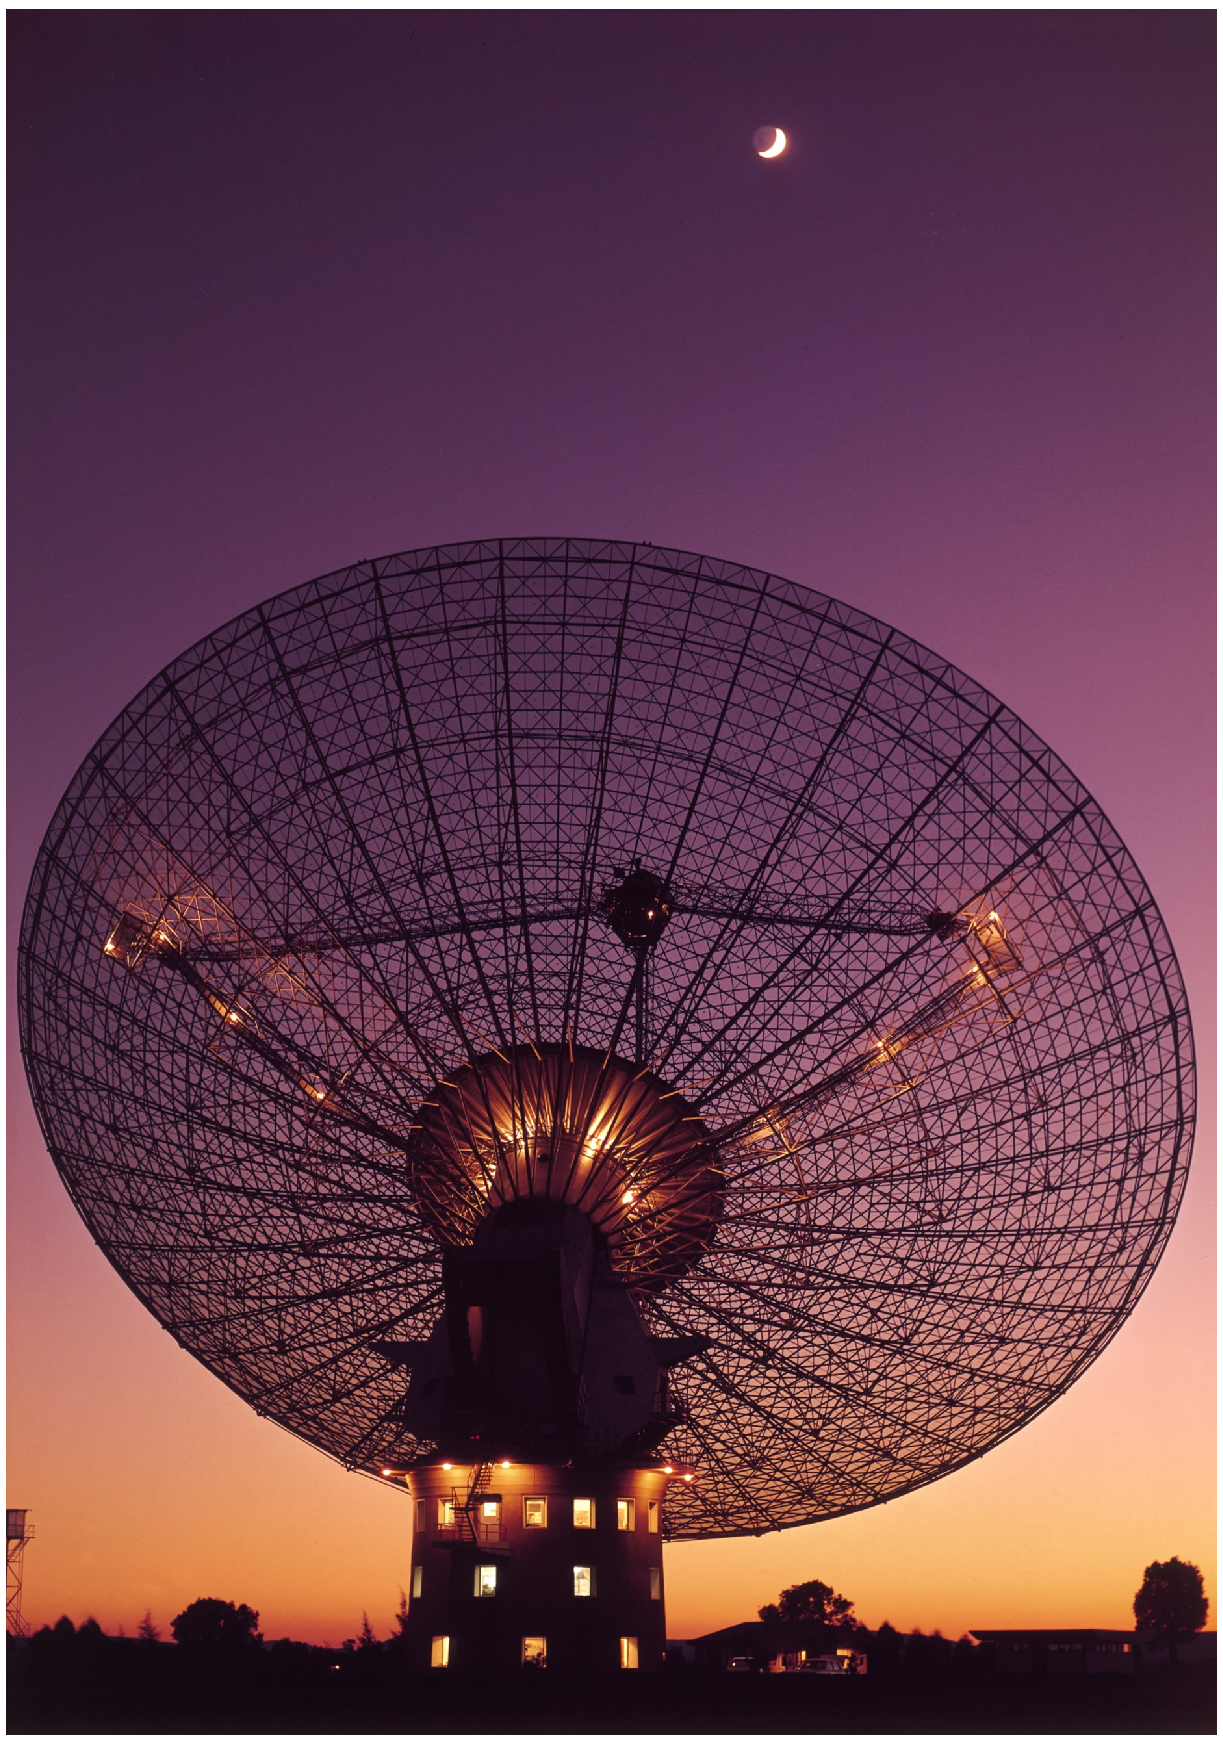
\includegraphics[width=\paperwidth]{background3.pdf}};%here you change your bookcover background
\draw (current page.center) node [fill=ocre!30!white,fill opacity=0.6,text opacity=1,inner sep=1cm]{\Huge\centering\bfseries\sffamily\parbox[c][][t]{\paperwidth}{\centering Apuntes sobre Telecomunicaciones\\[15pt] % Book title
{\Large Notas de un estudiante}\\[20pt] % Subtitle
{\huge Jose Antonio Hancco M.}}}; % Author name
\end{tikzpicture}
\vfill
\endgroup

%----------------------------------------------------------------------------------------
%	COPYRIGHT PAGE
%----------------------------------------------------------------------------------------

\newpage
~\vfill
\thispagestyle{empty}

\noindent Copyright \copyright\ 2022 Jose Hancco\\ % Copyright notice

\noindent \textsc{Libro libre de usos}\\ % Publisher

\noindent \textsc{https://github.com/Yasperterian}\\ % URL

\noindent Con licencia de Creative Commons Attribution-NonCommercial 3.0 Unported License (la ``Licencia''). No puede usar este archivo excepto de conformidad con la Licencia. Puede obtener una copia de la Licencia en \url{http://creativecommons.org/licenses/by-nc/3.0}. A menos que lo exija la ley aplicable o se acuerde por escrito, el software distribuido bajo la Licencia se distribuye \textsc{``tal cual'', sin garantías ni condiciones de ningún tipo}, ya sea expresa o implícita. Consulte la Licencia para conocer el idioma específico que rige los permisos y las limitaciones en virtud de la Licencia.\\ % License information, replace this with your own license (if any)

\noindent \textit{Primera edición, septiembre 2021} % Printing/edition date

\noindent Si existe algún error, crees que una sección se puede mejorar o dar cualquier tipo de \textit{feedback} acerca del libro no dudes y mándame un correo a \textit{jhanccoma@unsa.edu.pe}, te responderé lo más pronto que pueda y gracias por mejorar este libro de todos y para todos.
%----------------------------------------------------------------------------------------
%Dedicate
%----------------------------------------------------------------------------------------
\clearpage
\begin{center}
    \thispagestyle{empty}
    \vspace*{\fill}
    \textit{Ya sabes cómo funciona esto. Coges un libro, saltas a la dedicatoria y descubres que, una vez más, el autor ha dedicado su libro a alguien que no eres tú.\\
    Pero esta vez no será así...\\
    Dedico este libro a mi yo del pasado, quien ha sacrificado tiempo para poder escribir este libro para quienes lo necesiten pues como cualquier carrera, no es difícil los temas que tienes que aprender, sino que te lo explican mal y sin ganas, ganas desganadas que destruyen las tuyas. En consecuencia haces que quieras aprender para el examen, tan solo aprobar y obtener tus créditos. Espero hacer que lo temas te sean explicador bien (o al menos intentarlo) para que luego no sean difíciles los cursos posteriores.\\
    A lo largo de mi paso por la carrera de Ingeniería en Telecomunicaciones me han tocado cursos de contenido más que interesante pero con algunos docentes más paupérrimos (no todos, he tenido excelentes docentes con dedicación). Es en este contexto donde tu educación depende de ti y tus libros. Espero apoyar a esa causa de auto-educación para poder hacerte comprender algunos temas que realmente son muy complejos. No tengo la intención de que este sea un libro académico para que alguien lo use como fuente confiable; este libro es como su nombre lo dice: un cuaderno de apuntes que he ido recolectando a lo largo del tiempo.}
    \vspace*{\fill}
\end{center}
\clearpage
%----------------------------------------------------------------------------------------
%	TABLE OF CONTENTS
%----------------------------------------------------------------------------------------

%\usechapterimagefalse % If you don't want to include a chapter image, use this to toggle images off - it can be enabled later with \usechapterimagetrue

\chapterimage{chapter_head_generalindex.pdf} % Table of contents heading image

\pagestyle{empty} % Disable headers and footers for the following pages

\tableofcontents % Print the table of contents itself

\cleardoublepage % Forces the first chapter to start on an odd page so it's on the right side of the book

\pagestyle{fancy} % Enable headers and footers again
%----------------------------------------------------------------------------------------
%	PART
%----------------------------------------------------------------------------------------
\section*{Libros recomendados:}
\begin{itemize}
\item Fundamentos de circuitos eléctricos\cite{alexander2013fundamentos}
\item Signals and Systems Using MATLAB\cite{chaparro2018signals}
\item Procesamiento de señales analógicas y digitales\cite{ambardar1995analog}
\item Física Para Ciencias E Ingeniería. Vol 1\cite{serway2018fisica1}
\item Física Para Ciencias E Ingeniería. Vol 2\cite{serway2018fisica2}
\item Cálculo de una variable: trascendentes tempranas. 7ma edición \cite{stewart12calculo}
\item Análisis de Fourier\cite{hsu1998analisis}
\item Matemáticas Avanzadas Para Ingeniería\cite{o2014matematicas}
\item Métodos numéricos para ingenieros\cite{chapra2013metodos}
\item Comunicaciones y redes de computadores\cite{stallings2004comunicaciones}
\item Electrónica: teoría de circuitos y dispositivos electrónicos\cite{boylestad1989electronica}
\item Fundamentos de sistemas digitales\cite{floyd2006fundamentos}
\item Tratamiento de señales en tiempo discreto\cite{oppenheim2011tratamiento}
\item Tratamiento digital de señales\cite{proakis2007tratamiento}
\item Sistemas de comunicación digitales y análogos\cite{couchsistemas}
\item Data communication and networking\cite{forouzan2007data}
\item Life Pre-Intermediate 2e\cite{hughes2017life}
\item Redes de computadoras\cite{tanenbaum2012computer}
\item Líneas de transmisión\cite{velalineas1999}
\end{itemize}
\part{Electrotécnia}
\chapterimage{chapter_head_Elec.pdf}
\chapter{Números complejos}\index{Números complejos}
\begin{definition}[Módulo y Argumento]
Dado un número complejo $z=a+\iu b$, se define el \textbf{módulo} de $z$ como:
\begin{equation}
|z|=\sqrt{a^2+b^2}
\end{equation}
Se define el argumento de $z$ como:
\begin{equation}
arg(z)=\theta=arctg=\frac{b}{a}, a\neq 0
\label{eq:argumento}
\end{equation}
Tener en cuenta 3 puntos importantes:
\begin{enumerate}
\item La función arctg solo dará valores entre $45^{\circ}$ y -$45^{\circ}$.
\item Observar que, por ejemplo, la función arcotangente proporciona el mismo ángulo para $z=a-\iu b$ y para $w=-a+\iu b$. Sin embargo, $z$ y $w$ están en cuadrantes distintos, así que su argumento es distinto. Para solucionar esto:
\begin{itemize}
\item Si el complejo está en el \textbf{segundo cuadrante} $(a<0, b>0)$, hay que \textbf{sumar} $180^{\circ}$ ó $\pi$\footnote{Dependiendo del sistema angular en el que se este trabajando} al ángulo \textit{theta} obtenido en \ref{eq:argumento}.
\item Si el complejo está en el \textbf{tercer cuadrante} $(a<0, b<0)$, hay que \textbf{restar} $180^{\circ}$ ó $\pi$ al ángulo \textit{theta} obtenido en \ref{eq:argumento}.
\end{itemize}
\item Si a=0, el argumento es:
\begin{itemize}
\item $0^{\circ}$ (0 radianes) si $b=0$
\item $90^{\circ}$ ($\pi/2$ radianes) si $b>0$
\item $270^{\circ}$ ($3\pi/2$ radianes) si $b<0$
\end{itemize}
\end{enumerate}
Además, se denomina \textbf{argumento principal} de $z$, $Arg(z)$, al argumento de $z$ en el intervalo $]-180^{\circ},180^{\circ}]$ o, si es en radianes $]-\pi,\pi]$
\end{definition}
Sea el número complejo:
\begin{equation}
\label{art:numeroscomplejos}
A=10 + j5
\end{equation}
El número se puede expresar de distintas maneras:
\begin{align*}
\intertext{\textbf{Forma binómica}}
A&=\Re(A) + j\Im(A)\\
&\therefore A=10 + j5\\
\intertext{\textbf{Forma polar}}
A&=C\cdot e^{j\theta}, donde:\\
&\Rightarrow C=\sqrt{\Re(A)^2 + \Im(A)^2}\hspace{10pt}\theta=\tan^{-1}\left(\frac{\Im(A)}{\Re(A)}\right)\\
&\therefore C=\sqrt{10^2+5^2}=11.18\hspace{10pt}\theta=\tan^{-1}\left(\frac{5}{10}\right)=26.56^{\circ}\\
&\Rightarrow A=11.18\cdot e^{j 26.56}\\
\intertext{\textbf{Identidad de Euler}}
A&=C\cdot\cos\theta+jC\sin\theta=C(\cos\theta+j\sin\theta)\\
&\therefore A=11.18(\cos 26.56+j\sin 26.56)\\
\intertext{\textbf{Forma polar-Tipo fasor}}
A&=\fase{C}{\theta}\\
&\therefore A=\fase{11.18}{26.56}
\end{align*}
\begin{remark}
Las siguientes operaciones se realizarán usando como sistema angular los sexágesimales, en la calculadora no olvidarse de cambiar D (grados sexagesimales) a R (radianes). Con respecto a \textbf{theta} se puede trabajar con ambos sistemas siempre y cuando se especifique el sistema (° ó  rad). Es exclusivamente en la raíz cuadrada de complejos donde se debe trabajar \textit{theta} y su arctan, coseno, seno en \textbf{radianes} hasta obtener sus respuesta binómica desde donde ya se puede escoger el sistema en el que se expresará en su forma fasorial.
\end{remark}
\section{Operaciones con complejos}
\begin{itemize}
\item \textbf{Suma}:
\begin{align*}
(a+\iu b)&+(c+\iu d)\\
(a+c)&+\iu(b+d)
\end{align*}
\item \textbf{Resta}:
\begin{align*}
(a+\iu b)&-(c+\iu d)\\
(a-c)&+\iu(b-d)
\end{align*}
\item \textbf{Multiplicar}:
\begin{align*}
(a+\iu b)(c+\iu d)&=(a\cdot c-b\cdot d)+\iu(b\cdot c+a\cdot d)
\end{align*}
La forma más fácil de multiplicar es operando los números complejos en forma de \textbf{polar}/fasorial:
\begin{align*}
A&=Ce^{\iu\theta}=\fase{C}{\theta}\\
B&=De^{\iu\phi}=\fase{D}{\phi}\\
\end{align*}
El producto entre A y B esta definido por:
\begin{align*}
A\cdot B&=(\fase{C}{\theta})\cdot(\fase{D}{\phi})\\
A\cdot B&=(C\cdot D)\phase{\theta+\phi}
\end{align*}
\item \textbf{Dividir}:
\begin{align*}
\frac{a+\iu b}{c+\iu d}&=\frac{a+\iu b}{c+\iu d}\cdot\frac{c-\iu d}{c-\iu d}\\
\frac{a+\iu b}{c+\iu d}&=\frac{(a\cdot c+b\cdot d)+(b\cdot c-a\cdot d)\iu}{c^2+d^2}
\end{align*}
La forma más fácil de dividir es operando los números complejos en forma de \textbf{polar}/fasorial:
\begin{align*}
A&=Ce^{\iu\theta}=\fase{C}{\theta}\\
B&=De^{\iu\phi}=\fase{D}{\phi}\\
\end{align*}
la división entre A y B esta definido por:
\begin{align*}
A/B&=(\fase{C}{\theta})/(\fase{D}{\phi})\\
A/B&=(C/D)\phase{\theta-\phi}
\end{align*}
\item \textbf{Potencias}: Sea $z$ un complejo, la $n$-ésima potencia de z es: elevar a la $n$ el modulo de $z$ y multiplicar $n$ veces el argumento de $z$:
\begin{equation*}
\left(\fase{R}{\theta}\right)^n=\left(R^n\right)\phase{n\cdot\theta}
\end{equation*}
Para usar la fórmula de \textbf{Moivre}, se trabaja con la identidad de Euler:
\begin{equation*}
\left(\cos\alpha+\iu\sin\alpha\right)^n=\cos\left(n\cdot\alpha\right)+\iu\sin\left(n\cdot\alpha\right)
\end{equation*}
\item \textbf{Raíces}: Las $n$ raíces de $z$ constituyen los vértices de un polígono regular de $n$ lados centrado en el origen del plano complejo.
\begin{equation*}
\sqrt[n]{z}=z^{\frac{1}{n}}=\lbrace|z|^{\frac{1}{n}}e^{\frac{\theta+2k\pi}{n}\iu}:0\geq k \geq n-1\rbrace
\end{equation*}
Para pasar a forma binómica, aplicamos Euler:
\begin{equation*}
|z|^{\frac{1}{n}}\cdot e^{\frac{\theta+2k\pi}{n}\iu}=|z|^{\frac{1}{n}}\left[\cos\left(\frac{\theta+2k\pi}{n}\right)+\iu\sin\left(\frac{\theta+2k\pi}{n}\right)\right]
\end{equation*}
\begin{figure}[H]
\centering
\subfloat[Raíces quintas de $z=\iu$]{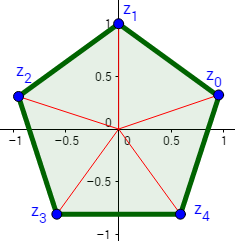
\includegraphics[width=0.3\linewidth]{Art/art2}}
\subfloat[Raíces cúbicas de $z=1+\iu$]{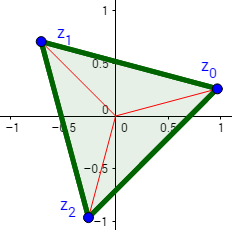
\includegraphics[width=0.3\linewidth]{Art/art3}}
\subfloat[Raíces cuartas de $z=1$]{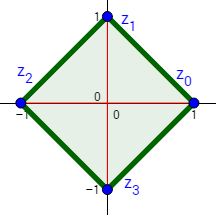
\includegraphics[width=0.3\linewidth]{Art/art4}}
\caption{Ejemplos de raíces complejas.}
\end{figure}
\end{itemize}
Este programa en python calcula las raices complejas de un número complejo.
\begin{python}
#Importamos librerias
import math
import matplotlib.pyplot as plt
import numpy as np
#Registramos los valores del usuario, de debe ingresar un complejo como: a+bj
number=complex(input("Ingresa el numero complejo: "))#Numero complejo
orden=int(input("Orden de la raiz: "))#Orden de la raiz
k=orden#Limite para la iteracion
if number.real==0:#Si la parte real es 0 se hacen excepciones para la indeterminacion
    if number.imag==0:
        theta=0
    elif number.imag>0:
        theta=math.pi/2
    elif number.imag<0:
        theta=3*math.pi/2
else:
    theta=math.atan(number.imag/number.real)#Thera calculada usando un arctg
valor=[]#Array de respuestas
#Bucle de iteracion
for i in range(0,k,1):
    r1=(abs(number)**(1/orden))*(math.cos((theta+2*i*math.pi)/(orden))+
        1j*math.sin((theta+2*i*math.pi)/(orden)))#Se calcula la rpta para cada valor de k
    valor.append(np.around(r1,4))#Se anade la respuesta al vector de respuestas y se redondea, el numero despues de r1 indica la cantidad de decimales
    print("Respuesta "+str(i))#Se imprime las respuestas
    print("------------------")
    print(valor[i])
    print("+++++++++++++++++++")
# Extraemos la parte real
x = [index.real for index in valor]
# Extraemos la parte imaginaria
y = [index.imag for index in valor]
ax = plt.gca()#Obtenemos las propiedades del plot
# plot the complex numbers
plt.scatter(x, y)#Ploteamos los puntos
plt.plot(x,y,color='b',zorder=1)#Unimos los puntos
plt.ylabel('Imaginary')#Rotulo de los ejes
plt.xlabel('Real')
plt.grid()#Activamos la grilla
for i_x, i_y in zip(x, y):#Obtenemos los valores para punto
    plt.text(i_x, i_y+0.02, '({}, j{})'.format(i_x, i_y))
plt.axvline(x=0, c="red")#Ploteamos los ejes del origen
plt.axhline(y=0, c="red")
plt.title("Raices complejas de "+str(number))#Anadimos titulos
plt.show()#Mostramos la grafica
\end{python}
\begin{remark}
Las operaciones de multiplicar y dividir un número complejo y un número real afecta tanto a la \textbf{parte real} como a la \textbf{parte imaginaria}:
\begin{align*}
(a+\iu b)\cdot k&=ak+\iu bk\\
(a+\iu b)\cdot k&=\frac{a}{k}+\iu \frac{b}{k}
\end{align*}
\end{remark}
\begin{definition}[Inverso de un complejo]
El sistema de los números complejos tiene la propiedad de la existencia del inverso multiplicativo o recíproco para todo número distinto de cero. La propiedad del inverso multiplicativo se refiere a que para cada número $z$, distinto de cero, existe un número, llamado el el inverso, denotado por $z^{-1}$, que cumple:
\begin{equation}
z\cdot z^{-1}=1
\end{equation}
Se puede demostrar que el inverso multiplicativo de $z=a+\iu b$ con $a\cdot b\neq 0$ es:
\begin{equation}
z^{-1}=\frac{a-\iu b}{a^2+b^2}
\end{equation}
El cual se obtiene de multiplicar al numerador y denominador por el \textbf{conjugado} del denominador:
\begin{align*}
\frac{1}{a+\iu b}&=\frac{a-\iu b}{(a+\iu b)(a-\iu b)}\\
&=\frac{a-\iu b}{a^2-(\iu b)^2}\\
&=\frac{a-\iu b}{a^2-b^2(\iu)^2}\\
&=\frac{a-\iu b}{a^2-b^2(-1)}\\
&=\frac{a-\iu b}{a^2+b^2}
\end{align*}
\end{definition}
\chapterimage{chapter_head_Elec.pdf}
\chapter{Dominio de la frecuencia}\index{Dominio de la frecuencia}\label{chap:dom freq}
\section{Fasores}\index{Fasores}
\begin{definition}[Fasor]
Es un número complejo que representa la amplitud y la fase de un senosoide.\\Usando la teoría de números complejos se puede escribir un número complejo Z=X+$\iu$Y en su forma fasorial:
\begin{equation}
Z=R\phase{\theta^{\circ}}
\end{equation}
Donde:
\begin{itemize}
\item R=$\sqrt{X^2+Y^2}$
\item $\theta$=$\arctan\left(\frac{Y}{X}\right)$
\end{itemize}
\end{definition}
Las operaciones entre fasores se realizan igual que cualquier complejo, se añade unas operaciones puntuales:
\begin{enumerate}
\item \textbf{Inverso}
\begin{displaymath}
\frac{1}{Z}=\frac{1}{R}\phase{-\theta}
\end{displaymath}
\item \textbf{Raíz cuadrada}
\begin{displaymath}
\sqrt{Z}=\sqrt{R}\phase{(\theta/2)}
\end{displaymath}
\item \textbf{Complejo conjugado}
\begin{displaymath}
Z^*=X-\iu Y=R\phase{-\theta}=R\cdot e^{-\iu\theta}
\end{displaymath}
\end{enumerate}
\subsection{Relación fasorial para R}
En el dominio del tiempo:
\begin{displaymath}
v(t)=R\cdot i(t)
\end{displaymath}
Forma polar:
\begin{displaymath}
V_m\phase{\theta}=RI_m\phase{\phi}
\end{displaymath}
Por lo tanto:
\begin{displaymath}
\mathbb{V}=R\mathbb{I}
\end{displaymath}
\begin{figure}[H]
\centering
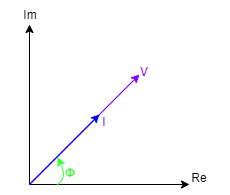
\includegraphics[width=0.5\linewidth]{Electro/Electro1.png}
\caption{Tensión y corriente están en fase}
\end{figure}
\begin{equation*}
\mathbb{I}=I_me^{\iu\phi}
\qquad
\mathbb{V}=RI_me^{\iu\phi}
\end{equation*}
\subsection{Relación fasorial para L}
Forma polar:
\begin{displaymath}
V_m\phase{\theta}=\iu\omega LI_m\phase{\phi}
\end{displaymath}
Por lo tanto:
\begin{displaymath}
\mathbb{V}=\iu\omega L\mathbb{I}
\end{displaymath}
\begin{figure}[H]
\centering
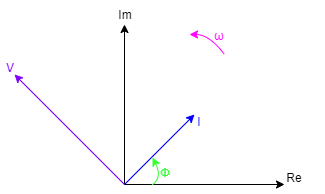
\includegraphics[width=0.5\linewidth]{Electro/Electro2.png}
\caption{Tensión adelantada respecto a la corriente en 90°}
\end{figure}
\begin{equation*}
\mathbb{I}=I_me^{\iu\phi}
\qquad
\mathbb{V}=\omega LI_me^{\iu(\phi+\pi/2)}
\end{equation*}
\subsection{Relación fasorial para C}
Forma polar:
\begin{displaymath}
I_m\phase{\phi}=\iu\omega CV_m\phase{\theta}
\end{displaymath}
Por lo tanto:
\begin{displaymath}
\mathbb{I}=\iu\omega C\mathbb{V}
\end{displaymath}
\begin{figure}[H]
\centering
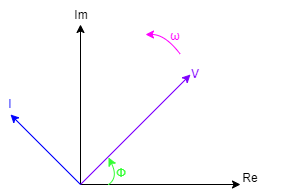
\includegraphics[width=0.5\linewidth]{Electro/Electro3.png}
\caption{Tensión retrasada respecto a la corriente en 90°}
\end{figure}
\begin{equation*}
\mathbb{I}=\omega CV_me^{\iu(\phi+\pi/2)}
\qquad
\mathbb{V}=V_me^{\iu\phi}
\end{equation*}
\begin{table}[H]
\begin{center}
\begin{tabular}{|c|c|}
\hline
\rowcolor[HTML]{34CDF9} 
Tiempo                     & Frecuencia                                  \\ \hline
$v(t)=R\cdot i(t)$         & $\mathbb{V}$=R$\mathbb{I}$                  \\ \hline
$v(t)=L\frac{di}{dt}$      & $\mathbb{V}$=$\iu\omega L\mathbb{I}$        \\ \hline
$v(t)=\frac{1}{C}\int idt$ & $\mathbb{V}=\frac{\mathbb{I}}{\iu\omega C}$ \\ \hline
\end{tabular}
\end{center}
\caption{Resumen de relaciones fasoriales}
\end{table}
\section{Impedancia}\label{Impedancia}
Las relaciones de tensión-corriente para los 3 elementos pasivos en el dominio de la frecuencia son:
\begin{equation*}
\mathbb{V}=\mathbb{R}\mathbb{I}
\qquad
\mathbb{V}=\iu\omega L\mathbb{I}
\qquad
\mathbb{V}=\frac{\mathbb{I}}{\iu\omega C}
\end{equation*}
La impedancia $\mathbb{Z}$ del elemento del circuito es el cociente entre la tensión fasorial $\mathbb{V}$ y la corriente fasorial $\mathbb{I}$:
\begin{displaymath}
\mathbb{Z}=\frac{\mathbb{V}}{\mathbb{I}}
\end{displaymath}
\begin{equation*}
\frac{\mathbb{V}}{\mathbb{I}}=R
\qquad
\frac{\mathbb{V}}{\mathbb{I}}=\iu\omega L
\qquad
\frac{\mathbb{V}}{\mathbb{I}}=\frac{1}{\iu\omega C}
\end{equation*}
Es una cantidad compleja que tiene dimensiones de \textbf{Ohms}, no es fasor y no puede transformarse al dominio del tiempo multiplicando por $e^{\iu\omega t}$ y tomando la parte real.
\begin{equation*}
\mathbb{Z}_R=R
\qquad
\mathbb{Z}_L=\iu\omega L
\qquad
\mathbb{Z}_C=\frac{1}{\iu\omega C}=-\iu\omega C
\end{equation*}
La \textbf{impedancia} es una función compleja de la frecuencia:
\begin{displaymath}
\mathbb{Z}=R+\iu X
\end{displaymath}
Donde R, X son reales.\\
La \textbf{parte real} de la impedancia se llama \textbf{resistancia}:
\begin{displaymath}
R=\Re[Z]
\end{displaymath}
La parte imaginaria es la \textbf{reactancia}, dentro la cual se distinguen 2:
\begin{displaymath}
X=\Im[Z]
\end{displaymath}
Si X es \textbf{positivo} se llama \textbf{inductancia}, si es negativo se llama \textbf{capacitancia}.
\begin{remark}
En C.A. la impedancia tiene un papel análogo a la resistencia en C.C.
\end{remark}
\begin{definition}[Asociación de impedancias]
Las dos asociaciones son\\
\textbf{Serie}:
\begin{equation}
Z_{eq}=Z_1+Z_2+\vdots+Z_n
\label{eq:serie impedancias}
\end{equation}
\textbf{Paralelo}:
\begin{equation}
\frac{1}{Z_{eq}}=\frac{1}{Z_1}+\frac{1}{Z_2}+\vdots+\frac{1}{Z_n}
\end{equation}
\end{definition}
\section{Admitancia}\label{Admitancia}
La admitancia es la inversa de la Impedancia, y consta al igual que ella con dos partes:
\begin{equation*}
\mathbb{Y}=G+\iu B=\frac{1}{\mathbb{Z}}=\frac{1}{R+\iu X}
\end{equation*}
La admintancia es puede ser hallada en base a la impedancia:
\begin{equation*}
\mathbb{G}=\frac{R}{R^2+X^2}
\qquad
\mathbb{B}=\frac{X}{R^2+X^2}
\end{equation*}
Proporción entre la corriente fasorial y la tensión fasorial medida en \textbf{Siemens}:
\begin{equation*}
\mathbb{Y}=\frac{\mathbb{I}}{\mathbb{V}}
\qquad
\mathbb{Y}=\frac{1}{\mathbb{Z}}
\end{equation*}
La parte real de la admitancia es la \textbf{conductancia}:
\begin{displaymath}
G=\Re[\mathbb{Y}]
\end{displaymath}
La parte imaginaria de la admitancia se llama \textbf{suceptancia}:
\begin{displaymath}
B=\Im[\mathbb{Y}]
\end{displaymath}
%----------------------------------------------------------------------------------------
%	PART
%----------------------------------------------------------------------------------------
\part{Métodos Matemáticos I}
\chapterimage{chapter_head_MM1.pdf}
\chapter{Ecuaciones Diferenciales de primer orden}
En este capítulo aprenderemos como resolver ecuaciones diferenciales. Para ello es necesario saber como siempre álgebra media-avanzada, cálculo diferencial e integral y sobre todo habilidad matemática. 
\section{Conceptos introductorios}\index{Conceptos introductorios}
Una ecuación diferencial es una ecuación derivada de una función desconocida(variable dependiente) respecto a una o más variables independientes.
\begin{displaymath}
\frac{dy}{dx}+5=e
\end{displaymath}
Donde:\\
y es nuestra variable \textbf{dependiente}.\\
x es nuestra variable \textbf{independiente}.\\
\subsection{Tipos}
Existen dos tipos de ecuaciones diferenciales.
\subsubsection{Ecuación diferencial Ordinaria}
Son de la forma:
\begin{displaymath}
dy=2dx
\end{displaymath}
\begin{displaymath}
\frac{dy}{dx}=2x
\end{displaymath}
\begin{displaymath}
\frac{dy}{dx}=2xy+3
\end{displaymath}
Donde nuestra prioridad es encontrar \textbf{y=F(x)}.
\subsubsection{Ecuación diferencial Parcial}
Estas ecuaciones son de la forma:
\begin{displaymath}
\frac{\partial u}{\partial x}+\frac{\partial u}{\partial y}=xy
\end{displaymath}
\begin{displaymath}
\frac{\partial ^2u}{\partial x^2}+\frac{\partial ^2u}{\partial y^2}=0
\end{displaymath}
Donde nuestra tarea es hallar \textbf{u=F(x,y)}
\subsection{Orden y grado}
Debemos dejar en claro algunos términos claro antes de proceder: Orden y Grado.
\subsubsection{Orden}
El orden de una ED\footnote{Desde ahora ecuación diferencial se abreviará como ED} es la derivada de mayor orden que aparece.
\subsubsection{Grado}
El grado de una ecuación diferencial (ya sea
ordinaria o parcial) es el exponente de la mayor
derivada contenida en la ecuación.
\begin{displaymath}
\overbrace{\underbrace{\left( \frac{d^3y}{dx^3}\right)^2}_{orden 3}}^{grado 2}-2\left(\frac{dy}{dx}\right)^4+xy=0
\end{displaymath}
\begin{definition}[Homogeneidad en funciones]
Una función en homogénea si todos los argumentos se multiplican por un factor constante, entonces el valor de la función resulta ser un cierto número de veces el factor multiplicativo elevado a una potencia. Dicha potencia es el grado de la función homogénea.
\begin{equation}\label{eq:homogeneidad}
G(tx,ty)=t^n\cdot G(x,y)\footnote{Se usará letras mayúsculas para representar funciones en su forma natural y letras minúsculas como las derivadas de las mismas.}
\end{equation}
Una función es homogénea si al multiplicarla por t nos devuelve la misma función multiplicada t a la n veces, donde n es el grado de homogeneidad.
\end{definition}
\begin{example}
Comprobar si la función F(x) es homogénea y si lo es, indicar su grado.
\begin{displaymath}
F(x,y)=\sqrt{x^2+y^2}
\end{displaymath}
\textbf{Solución}:\\
Multiplicamos por un mismo factor t.
\begin{displaymath}
F(tx,ty)=\sqrt{t^2x^2+t^2y^2}
\end{displaymath}
Factorizamos t de la expresión:
\begin{displaymath}
F(x,y)=t\overbrace{\sqrt{x^2+y^2}}^{F(x,y)}
\end{displaymath}
\begin{displaymath}
F(x,y)=t\cdot F(x,y)
\end{displaymath}
La función es homogénea de grado 1
\end{example}

\section{Variables separables}\index{Variables separables}
Son las más sencillas de identificar, para poder resolverlas es necesario hacer un despeje para ``acomodar" los términos e integrar a ambos lados de la expresión.
\begin{definition}[ED de variables separables]
La forma estándar de estas ecuaciones es:\\
\begin{displaymath}
\frac{dy}{dx}=F(x,y)=\frac{g(x)}{h(y)}
\end{displaymath}
\begin{displaymath}
\frac{dy}{dx}=\frac{g(x)}{h(y)}
\end{displaymath}
\begin{displaymath}
h(y)dy=g(x)dx \rightarrow \int h(y)dy=\int g(x)dx + C
\end{displaymath}
Después de la integración llegamos a:
\begin{displaymath}
H(y)=G(x)+C
\end{displaymath}
También pueden verse de la forma diferencial:\\
\begin{equation}\label{eq:edprimerorden}
G(x,y)dx+H(x,y)dy=0
\end{equation}
Ambas soluciones se presentan normalmente de la manera implícita.
\end{definition}
\begin{example}
\begin{equation}
\begin{split}
y\cdot ln(x)\frac{dx}{dy}&=\left(\frac{y+1}{x}\right)^2\\
\underbrace{\int x^2\cdot ln(x)dx}_{1}&=\underbrace{\int\frac{(y+1)^2}{y}dy}_{2}\\
\end{split}
\end{equation}
Resolviendo por integrales por partes para 1:\\
\begin{equation}
\begin{split}
u=ln(x)\hspace{35pt}du=\frac{1}{x}dx\\
dv=x^2\hspace{35pt}v=\frac{x^3}{3}\\
ln(x)\cdot\frac{x^3}{3}-\int\frac{x^3}{3}\cdot\frac{1}{x}dx\\
\frac{x^3\cdot ln(x)}{3}-\frac{x^3}{9}\\
\end{split}
\end{equation}
Resolviendo normalmente para 2:
\begin{equation}
\begin{split}
\int\left(\frac{y^2}{y}+\frac{2y}{y}+\frac{1}{y}\right)dy\\
\frac{y^2}{2}+2y+ln(y)\\
\end{split}
\end{equation}
Juntando los resultados de 1 y 2:\\
\begin{equation}
\boxed{\frac{x^3ln(x)}{3}-\frac{x^3}{9}=\frac{y^2}{2}+2y+ln(y)+C}
\end{equation}
\end{example}
%-----------------------------------------------------
\begin{example}
Ejercicio ED de primer orden con Condiciones Iniciales\footnote{Desde ahora se abreviará como C.I.}.
\begin{center}
\begin{equation}\label{eq:sinCI1}
\begin{split}
\frac{dy}{dt}+ty&=y;\thickspace y(1)=3\\
\frac{dy}{dt}&=y-ty\\
\frac{dy}{dt}&=y(1-t)\\
\int\frac{1}{y}dy&=\int\left(1-t\right)dt\\
ln(y)&=t-\frac{t^2}{2}+C
\end{split}
\end{equation}
\end{center}
De por sí, la ecuación \ref{eq:sinCI1} es la respuesta, pero por algo nos dan las C.I. Recordemos que \textit{y} es una función que depende de \textit{t}, en otras palabras:  Y(t). Con la C.I. que nos dieron, nos quiere decir que cuando \textit{t}=1, y vale 3. Bajo este pensamiento podemos seguir con el procedimiento(usando las ecuaciones \ref{art:expaln} y \ref{art:lnaexp}) para hallar C para la ecuación \ref{eq:sinCI1}.
\begin{center}
\begin{equation}\label{eq:CI1}
\begin{split}
y&=e^{t-\frac{t^2}{2}+C};\thickspace y(1)=3\\
3&=e^{1-\frac{1^2}{2}+c}\\
ln(3)&=\frac{1}{2}+C\\
ln(3)-\frac{1}{2}&=C\\
\end{split}
\end{equation}
\end{center}
Una vez despejada la ecuación de \ref{eq:CI1} podemos reemplazarla en la ecuación \ref{eq:sinCI1}:
\begin{equation}
\boxed{ln(y)=t-\frac{t^2}{2}+ln(3)-\frac{1}{2}}
\end{equation}
\end{example}
\begin{example}
Resolver la siguiente E.D.:\\
\begin{equation}\label{eq:exe3}
\frac{dy}{dx}=\frac{xy+3x-y-3}{xy-2x+4y-8}
\end{equation}
Factorizando y separando la ecuación \ref{eq:exe3}:
\begin{equation}
\begin{split}
\frac{dy}{dx}&=\frac{x(y+3)-(y+3)}{x(y-2)+4(y-2)}\\
\frac{dy}{dx}&=\frac{(y+3)(x-1)}{(y-2)(x+4)}\\
\frac{y-2}{y+3}dy&=\frac{x-1}{x+4}dx
\end{split}
\end{equation}
Desarrollando las divisiones de ambos lados:
%\polylongdiv[style=D]{6x^3-2x^2+x+3}{x^2-x+1}
\begin{equation}
\begin{split}
\int 1-\frac{5}{y+3}dy&=\int 1-\frac{5}{x+4}dx\\
y-5ln|y+3|&=x-5ln|x+4|+C
\end{split}
\end{equation}
Usando propiedad de los logaritmos(\ref{art:logaritmos}):
\begin{equation}
ln|x+4|^5-ln|y+3|^5=x-y+C
\end{equation}
Usando la propiedad de logaritmos(\ref{art:logdiv}):
\begin{equation}
\begin{split}
ln\left(\frac{x+4}{y+3}\right)^5&=x-y+C\\
\left(\frac{x+4}{y+3}\right)^5&=e^{x-y}\cdot e^C
\end{split}
\end{equation}
En este caso, una exponencial de \textit{c} es posible solo expresarla como una exponencial con exponente 1:
\begin{equation}
\boxed{\left(\frac{x+4}{y+3}\right)^5=e^{x-y}\cdot e}
\end{equation}
\end{example}
%\polylongdiv[style=D]{6x^3-2x^2+x+3}{x^2-x+1}
\section{Ecuaciones diferenciales lineales}\index{Ecuaciones diferenciales lineales}
\begin{definition}[E.D.L.]
\textbf{Forma estándar:}\\
\begin{equation}\label{eq:edl}
\frac{dy}{dx}+P(x)y=Q(x)
\end{equation}
Si Q(x)=0, la E.D. \ref{eq:edl} es \textbf{homogénea}\\
Si Q(x)$\neq$ 0, la E.D. \ref{eq:edl} \textbf{NO es homogénea}.
\end{definition}
Para resolver este tipo de E.D. necesario un cambio de variable que se demuestra de la siguiente manera:
\begin{equation}\label{eq:demo1}
\frac{d}{dx}\left[e^{\int P(x)dx}\cdot y\right]\\
\end{equation}
Derivando el producto de funciones:
\begin{equation*}
e^{\int P(x)dx}\cdot y+e^{\int P(x)dx}\cdot\frac{dy}{dx}
\end{equation*}
Acomodando los términos:
\begin{equation}\label{eq:demo2}
e^{\int P(x)dx}\left[P(x)y+\frac{dy}{dx}\right]
\end{equation}
Tengamos en cuenta la igualdad entre las ecuaciones \ref{eq:demo1} y \ref{eq:demo2}, por lo que es posible reemplazarla:
\begin{equation}\label{eq:ydespejadaedl}
\begin{split}
\underbrace{\left[P(x)y+\frac{dy}{dx}\right]e^{\int P(x)dx}}_{Ecuacion\ref{eq:demo1}}&=Q(x)\cdot e^{\int P(x)dx}\\
\frac{d}{dx}\left[e^{\int P(x)dx}\cdot y\right]&=Q(x)\cdot e^{\int P(x)dx}\\
\textup{Integrando a ambos lados}\\
\int \frac{d}{dx}\left[e^{\int P(x)dx}\cdot y\right]&=\int Q(x)\cdot e^{\int P(x)dx}\\
e^{\int P(x)dx}\cdot y&=\int Q(x)\cdot e^{\int P(x)dx}\\
\textup{Despejando y:}\\
y&=\frac{\int Q(x)\cdot e^{\int P(x)dx}dx}{e^{\int P(x)dx}}+C
\end{split}
\end{equation}\label{eq:cambiovariableu}
Haremos un cambio de variable:
\begin{equation}\label{eq:uedl}
\boxed{U(x)=e^{\int P(x)dx}}
\end{equation}
Haciendo el cambio de variable de la ecuación \ref{eq:cambiovariableu} en el resultado de la ecuación \ref{eq:ydespejadaedl} se obtiene:
\begin{equation}\label{eq:formageneraledl}
\boxed{U(x)Y(x)=\int Q(x)U(x)dx+C}
\end{equation}
En conclusión, para resolver una ecuación diferencial, se usa la ecuación \ref{eq:formageneraledl}, teniendo en cuenta el cambio de variable de la ecuación \ref{eq:uedl}.
\begin{example}
Resolver la siguiente E.D.L.:\\
\begin{displaymath}
\left(1-x^2\right)\frac{dy}{dx}-x=-xy
\end{displaymath}
Para resolver esta E.D.L. es necesario darle la forma a la ecuación, osea ordenar los términos y encontrar las funciones P(x) y Q(x) de acuerdo a la ecuación \ref{eq:edl}. En este caso tenemos que aislar la diferencial(\textit{$\frac{dy}{dx}$}), es por ello que dividimos todo entre ese término que acompaña a la diferencial. Luego hemos intercambiado los términos para tener del lado izquierdo la diferencial y una función que multiplique a \textit{y}, mientras que del lado derecho tenemos que tener solo una función:
\begin{equation}
\begin{split}
\left(1-x^2\right)\frac{dy}{dx}-x&=-xy\\
\frac{dy}{dx}+\frac{x}{(1-x^2)}y&=\frac{x}{(1-x^2)}
\end{split}
\end{equation}
\begin{displaymath}
P(x)=\frac{x}{(1-x^2)}\hspace{25pt}Q(x)=\frac{x}{(1-x^2)}
\end{displaymath}
Una vez que tenemos identificamos las funciones P(x) y Q(x), tenemos que usar el cambio de variable(ecuación \ref{eq:uedl}). Antes de seguir resolviendo la ecuación principal, resolvamos el cambio de variable. Para ello integramos la función P(x) como manda la ecuación \ref{eq:uedl}:
\begin{displaymath}
\begin{split}
\int \frac{x}{(1-x^2)}dx&=-\frac{1}{2}ln|1-x^2|\\
\therefore e^{\int P(x)dx}&=(1-x^2)^{-\frac{1}{2}}=U(x)
\end{split}
\end{displaymath}
La solución anterior, si es un poco complicada de comprender, se uso la propiedad \ref{art:logexp}.
Una vez que tenemos la función U(x), volvemos a la resolución principal, usando la función U(x) procedemos con la ecuación \ref{eq:formageneraledl} (despejamos Y(x), para ellos dividimos a ambos entre U(x)):
\begin{equation*}
\begin{split}
Y(x)&=\frac{\int\frac{x}{(1-x^2)}\cdot\frac{1}{\sqrt{1-x^2}}dx}{\frac{1}{\sqrt{1-x^2}}}+C\\
Y(x)&=\frac{\int\frac{x}{(1-x^2)^{\frac{3}{2}}} dx}{\frac{1}{\sqrt{1-x^2}}}+C\\
Y(x)&=\frac{-\cancel{\frac{1}{2}}\cdot\cancel{2}(1-x^2)^{-\frac{1}{2}} +C}{(1-x^2)^{-\frac{1}{2}}}
\end{split}
\end{equation*}
Separando el denominador para cada término del numerador:
\begin{equation}
\boxed{Y(x)=1+C(1-x^2)^{\frac{1}{2}}}
\end{equation}
\end{example}
\section{Ecuaciones Diferenciales Exactas}\index{Ecuaciones Diferenciales Exactas}
Este tipo de ecuaciones toman como referencia a las ecuaciones diferenciales de primer orden.
\begin{definition}[Ecuaciones Diferenciales exactas]
En base a la ecuación \ref{eq:edprimerorden}, se busca la siguiente forma estándar para poder resolver:
\begin{equation}\label{eq:edexacta}
M(x,y)dx+N(x,y)dy=0
\end{equation}
Será exacta si cumple con la siguiente condición:
\begin{equation}\label{eq:edecondicion}
\frac{\partial M(x,y)}{\partial y}=\frac{\partial N(x,y)}{\partial x}
\end{equation}
\end{definition}
\textbf{¿Cómo resolverla?}\\
Si hemos comprobado que nuestra ecuación diferencial es exacta usando la ecuación \ref{eq:edecondicion}, entonces existe una función \textit{F(x,y)} tal que:
\begin{subequations}
\begin{align}
\frac{\partial F(x,y)}{\partial x}=M(x,y)
\label{eq:edecondicion1} \\
\frac{\partial F(x,y)}{\partial y}=N(x,y)\label{eq:edecondicion2}
\end{align}
\label{eq:edecondiciones}
\end{subequations}
En la ecuación \ref{eq:edecondicion1} podemos determinar F(x,y) si integramos M(x,y) respecto a \textit{x}, obviamente manteniendo a \textit{y} como una constante. Si lo hacemos obtendremos:
\begin{equation}\label{eq:integrandomxy}
F(x,y)=\int M(x,y)dx+\textcolor{red}{G(y)}
\end{equation}
Añadimos la función \textcolor{red}{\textit{G(y)}} porque es una función de \textit{y} implícita, es decir existe ahi, pero como derivamos en función a \textit{x}, esta función \textcolor{red}{\textit{G(y)}} desaparece porque \textit{y} es considerada constante.\\
De la ecuación \ref{eq:integrandomxy}, ahora derivamos respecto a \textit{y} e igualamos este resultado con la ecuación \ref{eq:edecondicion2}:
\begin{subequations}
\begin{align}
\frac{\partial F(x,y)}{\partial y}=\frac{\partial}{\partial y}\left(\int M(x,y)dx\right)+g'(y)&=N(x,y)
\label{eq:derivarydem} \\
g'(y)&=N(x,y)-\frac{\partial}{\partial y}\left(\int M(x,y)dx\right)
\label{eq:despejeg}
\end{align}
\label{eq:despejegdex}
\end{subequations}
Ahora integraremos la ecuación \ref{eq:despejeg} respecto a \textit{y} y reemplazamos en la ecuación \ref{eq:integrandomxy}. Con eso ya estaría resuelta la ecuación diferencial exacta. La solución general se da de la siguiente manera:
\begin{displaymath}
F(x,y)=C
\end{displaymath}
\begin{example}
Resolver:
\begin{displaymath}
2y^2x-3dx+2yx^2+4dy=0
\end{displaymath}
Antes de todo, identifiquemos las funciones M y N en nuestra E.D.E:
\begin{displaymath}
\underbrace{2y^2x-3dx}_{M(x,y)}+\underbrace{2yx^2+4dy}_{N(x,y)}=0
\end{displaymath}
Trata de guiarte por las diferenciales(dx y dy) para identificarlas bien. Ahora tenemos que comprobar que se trata de una E.D.E:
\begin{equation}
\frac{\partial M}{\partial y}=4xy=\frac{\partial N}{\partial x},\therefore\text{es exacta}.
\end{equation}
Como es exacta, existe una función F(x,y), así que seguimos los pasos descritos anteriormente.\\
Empezamos con la ecuación \ref{eq:edecondicion1}:
\begin{equation}\label{eq:ejemploede1}
\begin{split}
\frac{\partial F(x,y)}{\partial}&=2y^2x-3\\
F(x,y)&=\int 2y^2x-3dx+G(y)\\
F(x,y)&=y^2x^2-3x+G(y)
\end{split}
\end{equation}
Ya tenemos la respuesta, pero debemos hallar G(y) para poder reemplazarla en \ref{eq:ejemploede1}. En consecuencia seguimos con el paso detallado en la ecuación \ref{eq:edecondicion2}:
\begin{equation}\label{eq:condicion2ejemplo}
\frac{\partial F(x,y)}{\partial y}=2yx^2+4
\end{equation}
Lo que vamos a hacer es lo siguiente: Nosotros ya tenemos F(x,y) (ecuación \ref{eq:ejemploede1}) pero nos falta hallar G(y), es por ello que hallamos el término de N(x,y)(ecuación \ref{eq:edecondicion2}). Ese termino nos dice que si realizamos la derivada parcial respecto a \textit{y} a la función F(x,y) obtendremos N(x,y). Nosotros tenemos F(x,y) y tenemos N(x,y); y tenemos una función desconocida que depende de \textit{y}(G(y)), por consecuencia, hallaremos esa función desconocida:
\begin{subequations}
\begin{align}
\frac{\partial F(x,y)}{\partial y}=2yx^2+g'(y)&=2yx^2+4
\label{eq:ejemploede2} \\
g'(y)&=4
\label{eq:ejemploede3} \\
\int g'(y)dy&=\int 4dy 
\label{eq:ejemploede4} \\
G(y)&=4y
\label{eq:ejemploede5}
\end{align}
\end{subequations}
\textbf{¿Qué se hizo?}\\
Por si te cuesta entender, vamos a detallar:
\begin{enumerate}
\item \textbf{Ecuación \ref{eq:ejemploede2}}: Hallamos el termino correspondiente a la expresión \ref{eq:edecondicion2}, que es la expresión \ref{eq:condicion2ejemplo}; si nos centramos solo en esta expresión nos dice que: la derivada parcial de F(x,y) respecto a \textit{y} es N(x,y). Nosotros sabemos cuanto vale N(x,y) pero no sabemos cuando vale F(x,y). Pero, si nos fijamos bien, sabemos cuanto vale F(x,y)(ecuación \ref{eq:ejemploede1}), y si la derivamos podemos igualar a la expresión \ref{eq:condicion2ejemplo}.
\item \textbf{Ecuación \ref{eq:ejemploede3} y \ref{eq:ejemploede4}}: Ya hallamos \textit{g'(x)}, así que solo nos queda integrar \textbf{respecto a \textit{y}} porque es una función de \textit{y}.
\end{enumerate}
Ahora que tenemos todo: solo nos queda reemplazar en la ecuación \ref{eq:ejemploede1} el valor de la función incógnita \textit{G(y)} hallada en\ref{eq:ejemploede5}:
\begin{equation}
\boxed{F(x,y)=y^2x^2-3x+4y=C}
\end{equation}
\end{example}
\begin{remark}
Se puede cambiar el orden de resolver, es decir, primero hemos resuelto la expresión \ref{eq:edecondicion1} y luego la expresión \ref{eq:edecondicion2}, pero también es valido(y debería salir lo mismo) si haces primero la expresión \ref{eq:edecondicion2} y luego la expresión \ref{eq:edecondicion1}
\end{remark}
\section{Ecuaciones Diferenciales No Exactas}\index{Ecuaciones Diferenciales No Exactas}
Este tipo de E.D.N.E son reducibles a E.D.E mediante un factor integrante.
\begin{definition}[Ecuaciones Diferenciales exactas]
En base a la ecuación \ref{eq:edprimerorden}, se busca la siguiente forma estándar para poder resolver:
\begin{displaymath}
M(x,y)dx+N(x,y)dy=0
\end{displaymath}
Será exacta si cumple con la siguiente condición:
\begin{equation}\label{eq:edecondicion}
\frac{\partial M(x,y)}{\partial y}\neq\frac{\partial N(x,y)}{\partial x}
\end{equation}
\end{definition}
\textbf{¿Cómo resolver?}\\
Tenemos que buscar un F.I.\footnote{Abreviación de Factor Integrante} para que la E.D.N.E se haga E.D.E.\\
Si:
\begin{equation}
\frac{1}{N(x,y)}\left(\frac{\partial M(x,y)}{\partial y}-\frac{\partial N(x,y)}{\partial x}\right)
\label{eq:ednecondicion1}
\end{equation}
devuelve como resultado una función que \textbf{SOLO} depende de \textbf{\textit{x}}; entonces el F.I. es:
\begin{equation}
U(x)=e^{\int \frac{1}{N(x,y)}\left(\frac{\partial M(x,y)}{\partial y}-\frac{\partial N(x,y)}{\partial x}\right)dx}
\label{eq:fix}
\end{equation}
Si:
\begin{equation}
\frac{1}{M(x,y)}\left(\frac{\partial N(x,y)}{\partial x}-\frac{\partial M(x,y)}{\partial y}\right)\label{eq:ednecondicion2}
\end{equation}
devuelve como resultado una función que \textbf{SOLO} depende de \textbf{\textit{y}}; entonces el F.I. es:
\begin{equation}
U(y)=e^{\int \frac{1}{M(x,y)}\left(\frac{\partial N(x,y)}{\partial x}-\frac{\partial M(x,y)}{\partial y}\right)dy}
\label{eq:fiy}
\end{equation}
Cuando se hallada multiplicamos a toda la E.D.N.E por F.I.; haciendo esto la E.D pasará a ser una E.D.E. y se procede a resolver como tal.
\begin{example}
Resolver:
\begin{displaymath}
xydx+\left(2x^2+3y^2-20\right)dy=0
\end{displaymath}
\textbf{Solución:}\\
Queda de más que antes de todo, es necesario identificar M(x,y) y N(x,y):
\begin{displaymath}
\underbrace{xy}_{M(x,y)}dx+\underbrace{\left(2x^2+3y^2-20\right)}_{N(x,y)}dy=0
\end{displaymath}
Como primer paso, tenemos que ver si se trata de una E.D exacta o no exacta:
\begin{equation}
\left.
\frac{\partial M(x,y)}{\partial y}=x \atop
\frac{\partial N(x,y)}{\partial x}=4x
\right\}\neq \therefore\textup{La E.D. no es exacta}
\end{equation}
Procedemos con la solución de esta E.D.N.E., por lo tanto tendremos que hallar el F.I.. Empezaremos con la ecuación \ref{eq:ednecondicion1}\footnote{Puedes empezar con la ecuación \ref{eq:ednecondicion1} o \ref{eq:ednecondicion2}, de notas formas, si una no cumple la condición usas la otra.}
\begin{displaymath}
\frac{1}{\left(2x^2+3y^2-20\right)}\left(\frac{\partial(xy)}{\partial y}-\frac{\partial\left(2x^2+3y^2-20\right)}{\partial x}\right)=\frac{-3x}{2x^2+3y^2-20}
\end{displaymath}
Aqui tenemos un problema, se supone que la función resultante solo debe depender de \textit{x}, pero la nuestra depende de \textit{y} también. Descartamos esta.\\
Como esta primera comprobación para hallar F.I. no cumple la condición probamos con la otra(ecuación \ref{eq:ednecondicion2}):
\begin{displaymath}
\frac{1}{xy}\left(\frac{\partial \left(2x^2+3y^2-20\right)}{\partial x}-\frac{\partial (xy)}{\partial y}\right)=\frac{3\cancel{x}}{\cancel{x}y}=\frac{3}{y}
\end{displaymath}
Este condicionante para hallar el F.I. solo depende de \textit{y}, así que nos sirve y por ende, trabajaremos con ese mismo, por lo que ahora hallaremos el F.I. según la expresión \ref{eq:fiy}:
\begin{equation}
U(y)=e^{\int\frac{3}{x}dy}=y^3
\end{equation}
Cuando se halla encontrado el F.I. multiplicamos a toda la E.D.N.E por U(x) para obtener una E.D.E.

\begin{equation}
\begin{split}
\textcolor{red}{y^3}(xydx+\left(2x^2+3y^2-20\right)dy&=0)\\
xy^4dx+\left(2x^2y^3+3y^5-20y^3\right)&=0
\end{split}
\end{equation}
Si en este momento procedemos a comprobar si es exacta, obtendremos:
\begin{equation*}
\frac{\partial M}{\partial y}=4xy^3=\frac{\partial N}{\partial x},\therefore\text{es exacta}.
\end{equation*}
Ahora podemos resolverla como lo hacemos para las E.D.E.:\\
\begin{displaymath}
\begin{split}
F(x,y)&=\int xy^4dx+G(y)\\
F(x,y)&=\frac{y^4x^2}{2}+G(y)\\
\end{split}
\end{displaymath}
Derivamos F(x,y) respecto a y e igualamos a N(x,y)
\begin{displaymath}
\begin{split}
\cancel{2y^3x^2}+g'(y)&=2x^2y^3+3y^5-20y^3\\
g'(y)&=3y^5-20y^3\\
G(y)&=y^6-5y^4\\
F(x,y)&=\frac{y^4x^2}{2}+\frac{y^6}{2}-5y^4=C
\end{split}
\end{displaymath}
Multiplicando por dos a toda la expresión, teniendo en cuenta que 2 es constante:
\begin{equation}
\boxed{y^4x^2+y^6-10y^4=C}
\end{equation}
\end{example}
\section{Ecuaciones por sustitución}\index{Ecuaciones por sustitución}
\subsection{Ecuaciones Homogéneas}
Recordando lo aprendido en la ecuación \ref{eq:homogeneidad}, una ecuación de la forma:
\begin{displaymath}
M(x,y)dx+N(x,y)dy=0
\end{displaymath}
será homogénea si M(x,y) y N(x,y) son homogéneas del mismo grado:
\begin{align*}
M(xt,yt)=t^nM(x,y) \hspace{20pt} N(xt,yt)=t^nN(x,y)\\
\end{align*}
o:
\begin{align*}
M(x,y)=x^nM(1,u) \hspace{20pt} N(x,y)=x^nN(1,u), \text{donde:}u=\frac{y}{x}
\end{align*}
Al final, tenemos que devolver el cambio de variable \textit{u}. Una ecuación diferencial homogénea siempre puede reducirse a una ecuación de variable separable por medio de una sustitución algebraica.\\
\textbf{¿Cómo se hace?}\\
Sea la ecuación diferencial de la forma \ref{eq:edexacta} y sea homogénea. Se reduce a una E.D de variable separable usando cualquiera de las sustituciones, recordando que \textit{u} y \textit{v} son las nuevas variables dependientes.:
\begin{subequations}
\begin{align}
y=u\cdot x
\label{eq:edhsustituciony} \\
x=v\cdot y
\label{eq:edhsustitucionx}
\end{align}
\end{subequations}
Si elegimos \textbf{y=u$\cdot$ x} con su derivada:
\begin{equation}\label{eq:yux}
y=u\cdot x\longrightarrow dy=udx+xdu
\end{equation}
Si reemplamos \ref{eq:yux} en \ref{eq:edexacta}:
\begin{displaymath}
M(x,\textcolor{red}{ux})dx+N(x,\textcolor{red}{ux})\underbrace{(udx+xdu)}_{dy}=0
\end{displaymath}
Aplicando la propiedad de homogeneidad a M y N es posible escribir:
\begin{displaymath}
x^nM(1,u)dx+x^nuN(1,u)dx+x^nxN(1,u)du=0
\end{displaymath}
\begin{displaymath}
x^n\left[M(1,u)+uN(1,u)\right]dx+x^nN(1,u)du=0
\end{displaymath}
Dividiendo a toda la expresión entre $x^n$
\begin{displaymath}
\left[M(1,u)+uN(1,u)\right]dx+N(1,u)du=0
\end{displaymath}
Si hacemos una división a nuestra conveniencia para arreglar la E.D.
\begin{displaymath}
\frac{dx}{x}+\frac{N(1,u)du}{M(1,u)+uN(1,u)}=0
\end{displaymath}
\begin{remark}
El procedimiento anterior no debe ser memorizado, puesto que es solo una ejemplo de como se debe realizar las sustituciones. El procedimiento debe hacerse por completo.
\end{remark}
La sustitución por \textbf{x=v$\cdot$y} se realiza de manera similar.\\
\textbf{Observaciones:}
\begin{enumerate}
\item En la practica, la sustitución de \textbf{x=v$\cdot$y} se elije cuando la función M(x,y) sea de estructura más simple que N(x,y).
\item Cuando no hay diferencia apreciable entre M y N 
, se puede usar cualquiera de los dos sustituciones.
\item Si al resolver la que escogimos vemos que se torna complicada(algebraicamente) usamos la otra sustitución.
\end{enumerate}
\begin{example}\label{eq:edhejemplo1}
Resolver:
\begin{equation}
(x-y)dx+xdy=0
\end{equation}
Si hacemos las propiedades de la homogeneidad, notaremos que son homogéneas en grado 1. Elegiremos:
\begin{equation}\label{eq:edhejemplo2}
\textbf{y=u$\cdot$x} \longrightarrow dy=udx+xdu
\end{equation}
Reemplazando \ref{eq:edhejemplo2} en \ref{eq:edhejemplo1}:
\begin{displaymath}
(x-ux)dx+x(udx+xdu)=0
\end{displaymath}
Dividimos toda la expresión entre \textit{x}:
\begin{displaymath}
(1-u)dx+(udx+xdu)=0
\end{displaymath}
Agrupando algebraicamente:
\begin{displaymath}
(1-u+u)dx+xdu=0 \longrightarrow  dx+xdu=0
\end{displaymath}
Dividimos entre x\footnote{Este paso depende de la función, recuerda que tenemos que buscar una E.D. de variable separable.}:
\begin{displaymath}
\frac{dx}{x}+du=0
\end{displaymath}
Esta expresión ya es una E.D. de variable separable:
\begin{displaymath}
\begin{split}
\int\frac{dx}{x}+\int du&=\int x\\
ln|x|+u&=c
\end{split}
\end{displaymath}
Devolviendo la variable \textit{u}:
\begin{equation*}
\boxed{ln|x|+\frac{y}{x}=C}
\end{equation*}
\end{example}
\subsection{Ecuaciones Diferenciales de Bernoulli}
Otro tipo de ecuación que se resuelven por sustitución son las ecuaciones diferenciales de Bernoulli.
\begin{definition}
La forma estándar de las E.D. de Bernoulli es:
\begin{subequations}
\begin{align}
\frac{dy}{dx}+P(x)\cdot y&=Q(x)\cdot y^n
\label{eq:edb1} \\
\frac{dx}{dy}+P(y)\cdot x&=Q(y)\cdot x^n
\label{eq:edb2}
\end{align}
\label{eq:edb}
\end{subequations}
\end{definition}
\begin{remark}
En algunos casos, pueden haber funciones que acompañen a las $\frac{dy}{dx}$, pero ya se trata de un trabajo algebraico en llegar a las expresiones \ref{eq:edb}.
\end{remark}
En ambos casos de las formas estándares \ref{eq:edb}, si n=0, y=1 en la ecuación \ref{eq:edb1} o x=1 en la ecuación \ref{eq:edb2} nos encontramos ante una E.D.L. y no hay problemas porque ya sabemos como resolver. Sin embargo si n$\neq$ 0, y$\neq$ 1 en la ecuación \ref{eq:edb1} o x$\neq$ 1 en la ecuación \ref{eq:edb2} nos encontramos frente a un E.D.B\footnote{Abreviación de Ecuación Diferencial de Bernoulli.}, estas E.D. se resuelven aplicando una sustitución.\\
El cambio de variable es:
\begin{equation}\label{eq:edbw}
W=1^{1-n}
\end{equation}
\textbf{¿Cómo se llega a ese cambio de variable?}\footnote{Obviamente en esta caso y$\neq$1 y n$\neq$0.}\\
\begin{displaymath}
\frac{dy}{dx}+P(x)y=Q(x)y^n
\end{displaymath}
Dividimos entre $y^n$:
\begin{equation}\label{eq:explicacionw1}
y^{-n}\frac{dy}{dx}+P(x)y^{1-n}=Q(x)
\end{equation}
Haciendo un cambio de variable con su derivada:
\begin{equation}\label{eq:explicacionw2}
\begin{split}
W=y^{1-n}\longrightarrow \frac{dw}{dx}&=(1-n)y^{-n}\cdot \frac{dy}{dx}\\
\frac{1}{(1-n)}\cdot \frac{dw}{dx}&=y^{-n}\cdot\frac{dy}{dx}
\end{split}
\end{equation}
Sustituyendo la expresión \ref{eq:explicacionw2} en \ref{eq:explicacionw1}:
\begin{displaymath}
\textcolor{red}{\frac{1}{(1-n})\cdot\frac{dw}{dx}}+P(x)\textcolor{red}{W}=Q(x)
\end{displaymath}
Multiplicando toda la expresión por (1-n):
\begin{displaymath}
\frac{dw}{dx}+\underbrace{(1-n)P(x)}_{M}W=\underbrace{(1-n)Q(x)}_{N}
\end{displaymath}
Ahora es una E.D.L. y se procede con su procedimiento aprendido.
\begin{example}
Resolver:
\begin{displaymath}
\left(4-x^2\right)\frac{dy}{dx}+4y=(2+x)y^2
\end{displaymath}
Buscamos una expresión similar a \ref{eq:edb1}:
\begin{displaymath}
\frac{dy}{dx}+\frac{4}{\left(4-x^2\right)}y=\frac{2+x}{\left(4-x^2\right)}y^2
\end{displaymath}
Dividimos entre $y^2$:
\begin{equation}\label{eq:edbex1}
y^{-2}\frac{dy}{dx}+\frac{4}{\left(4-x^2\right)}y^{-1}=\frac{2+x}{\left(4-x^2\right)}
\end{equation}
Efectuamos el cambio de variable W:
\begin{equation}\label{eq:edbex2}
\begin{split}
W=y^{1-2}\longrightarrow \frac{dw}{dx}&=(1-2)y^{-2}\cdot \frac{dy}{dx}\\
-\frac{dw}{dx}&=y^{-2}\cdot\frac{dy}{dx}
\end{split}
\end{equation}
Reemplazando la expresión \ref{eq:edbex2} en \ref{eq:edbex2}:
\begin{displaymath}
\begin{split}
-\frac{dw}{dx}+\frac{4W}{\left(4-x^2\right)}&=\frac{2+x}{4-x^2}\\
\frac{dw}{dx}+\frac{4}{\left(x^2-4\right)}\cdot W&=\frac{1}{x-2}
\end{split}
\end{displaymath}
Ahora se procede a resolver como una E.D.L.
\begin{equation*}
\begin{split}
U(x)&=e^{\int\frac{4}{(x-2)}dx}\\
U(x)&=e^{ln\left|\frac{x-2}{x+2}\right|}\\
U(x)&=\frac{x-2}{x+2}
\end{split}
\end{equation*}
\begin{equation*}
\begin{split}
\frac{x-2}{x+2}\cdot W(x)&=\int\frac{1}{\cancel{\left(x-2\right)}}\cdot\frac{\cancel{\left(x-2\right)}}{\left(x+2\right)}dx+C\\
W(x)&=\left[ln|x+2|+C\right]\cdot\frac{x+2}{x-2}\\
\end{split}
\end{equation*}
Devolviendo el cambio de variable $W=y^{(1-2)}$:
\begin{equation}
\boxed{y^{-1}=\left[ln|x+2|+C\right]\cdot\frac{x+2}{x-2}}
\end{equation}
\end{example}
%---------------------------------------------------------------
%Chapter separation
%---------------------------------------------------------------
\part{Sistemas Digitales}
\chapterimage{chapter_head_SD.pdf} % Chapter heading image
\chapter{Sistemas de numeración}
\index{Sistemas de numeración}
\section{Sistema decimal: 10}\index{Sistema decimal: 10}
El que todos conocemos, los números representados en este sistema tiene como base el número diez y sus múltiplos:
\begin{center}
\begin{tabular}{|c|c|c|c|c|c|c|}
\hline
6      & 5      & 4      & 3      & 2      & 1      & 0      \\ \hline
$10^6$ & $10^5$ & $10^4$ & $10^3$ & $10^2$ & $10^1$ & $10^0$ \\ \hline
\end{tabular}
\end{center}
Notamos en la primera fila el \textbf{la posición}, en la segunda fila sus potencias en \textbf{base 10} basadas en la posición. Y se sabe que un número cualquiera puede ser expresado en base de 10, con el cuadro anterior podemos deducir que:
\begin{displaymath}
\textcolor{red}{1}\textcolor{blue}{2}\textcolor{green}{7}=\textcolor{red}{1}\cdot 10^2 + \textcolor{blue}{2}\cdot 10^1 + \textcolor{green}{7}\cdot 10^0
\end{displaymath}
Los números en base 10 van desde el 0 hasta el 9, aunque se llame base 10, \textbf{NO} llega nunca el número 10, sino que el 10 es la combinación de 1 decena con 0 unidades.\\
En conclusión, el número se descompone en unidades, decenas, centenas, etc y se multiplica el valor de cada uno por la base correspondiente.
\subsection{Suma}
La suma se realiza columna por columna, recordando que el \textbf{límite} mayor es el 9, por ejemplo:
\begin{center}
\opadd{123}{19}
\end{center}
Si sumamos en la primera columna (de derecha a izquierda), 9 más 3 da 12 y decimos \textit{llevamos 1} porque ha rebasado el límite de 9 unidades, colocamos solo el número de la unidad y llevamos 1 hacia la otra columna y así sucesivamente con las demás columnas.
\subsection{Resta}
En la resta pasa algo similar, si tenemos el minuendo mayor que el sustraendo no habrá problemas, sin embargo cuando el sustraendo es mayor que el minuendo solemos hacer la jugada comúnmente llamada \textit{``nos prestamos''} de la siguiente columna.
\begin{center}
\opsub{123}{19}
\end{center}
Prestemos atención a esa simple ``jugada'',  en la resta presentada tenemos: 3-9, no podemos restar así que nos prestamos 1 del 2 de la siguiente columna, ahora tenemos 13-9, aquí tengo que \textbf{resaltar} que es lo que realmente se ha hecho: al ``prestarnos 1'' lo que se hizo es pasar un decena o 10 al número que lo necesite y poder efectuar la resta, es por eso que el 3 pasa a ser 13 porque como pasamos 10 queda: 10+3=13.\\
Ahora si podemos restar, 13-9 da 4; siguiente columna, el dos de donde nos ``prestamos'' pasa a ser 1 y en esta columna tendríamos 1-1 el cual da 0, por último bajamos el 1. En conclusión, al ``prestarnos'' lo que hacemos es pasar de una columna a otra un \textbf{valor de diez}.
\section{Sistema binario-2}\index{Sistema binario-2}
Aquí, el sistema esta basado en \textbf{potencias de 2} y los símbolos permitidos son solo el \textbf{0 y 1}. Funcionan al igual que los demás sistemas:
\begin{center}
\begin{tabular}{|c|c|c|c|c|c|c|c|}
\hline
7     & 6     & 5     & 4     & 3     & 2     & 1     & 0     \\ \hline
$2^7$ & $2^6$ & $2^5$ & $2^4$ & $2^3$ & $2^2$ & $2^1$ & $2^0$ \\ \hline
\end{tabular}
\end{center}
\begin{remark}
En este sistema no esta definido unidades, decenas o centenas, pues esos son propios del sistema decimal; en su lugar para identificarlos, cada valor es llamado \textbf{bit} y el bit que indica de donde se empieza a leer (en decimal se sobre-entiende que se lee de izquierda a derecha) se llama \textbf{bit más significativo} (MSB), usualmente es el que esta más a la izquierda pero hay aplicaciones donde cambia de posición; la contraparte del MSB es \textbf{bit menos significativo} (LSB) e indica el final del número.
\end{remark}
Aún no tocaremos las potencias de dos, eso lo veremos más adelante.\\
Es usual ver números en este sistema agrupados de 4 en 4 bits, pero no es obligatorio. \textbf{8 bits son iguales a 1 byte.}
\subsection{Suma}
Trabajamos igual que siempre, teniendo en cuenta los bits que rebasen el sistema, es decir:
\begin{itemize}
\item \textbf{0+0=0}
\item \textbf{0+1=1}
\item \textbf{1+0=1}
\item \textbf{1+1=10}, al igual que en binario, el cero lo colocamos en la respuesta y el 1 se convierte en acarreo para la siguiente columna, o en otras palabras: \textit{llevamos 1}.
\end{itemize}
\begin{center}
\par\vspace{2\oplineheight}
\oplput(1,2){1}\oplput(2,2){1}\oplput(3,2){0}
\oplput(0,1.5){$+$}
\oplput(1,1){0}\oplput(2,1){1}\oplput(3,1){1}
\ophline(0,0.8){4}
\oplput(0,0){1}\oplput(1,0){0}\oplput(2,0){0}\oplput(3,0){1}
\end{center}
\subsection{Resta}
La resta trabaja bajo la misma teoría, el límite es 1 aunque el sistema binario trabaje en base 2:
\begin{center}
\par\vspace{2\oplineheight}
\oplput(1,2){1}\oplput(2,2){0}\oplput(3,2){1}
\oplput(0,1.5){$-$}
\oplput(1,1){0}\oplput(2,1){1}\oplput(3,1){1}
\ophline(0,0.8){4}
\oplput(1,0){0}\oplput(2,0){1}\oplput(3,0){0}
\end{center}
Restamos de izquierda a derecha como sabemos:
\begin{enumerate}
\item 1-1: Da 0
\item 0-1: Aquí no podemos restar, hacemos un ``préstamo'' del 1 de la siguiente fila, ese préstamo lo que hace es darnos la base del sistema como vimos antes, aquí el préstamo haría 10 en binario (o 2 en decimal\footnote{Más adelante veremos conversiones}), tenemos dos opciones: ese préstamo nos dio un 2, sumamos 2+0 y tenemos 2, ahora lo restamos con el 1 u tenemos 1; la segunda opción es trabajar con binario, tendríamos 10 (1 del préstamo) y restamos 10-1=01, esta forma se entenderá  mejor más adelante.
\end{enumerate}
Como recurso final se puede usar las siguientes condiciones:
\begin{itemize}
\item \textbf{0-0=0}
\item \textbf{0-1=1}, con acarreo negativo en la siguiente columna
\item \textbf{1-0=1}
\item \textbf{1-1=0}
\end{itemize}
\subsection{Negativos}
Los negativos con un tanto confuso pero funcionan bajo una lógica simple, se poseen 4 formas de expresar los negativos: Signo-magnitud, complemento a 1, complemento a 2 y exceso:
\subsubsection{Signo-magnitud}
El bit más significativo (MSB) nos indicará si es positivo (0) o negativo (1). Si queremos pasar a decimal, ese uno que indica \textcolor{red}{negativo} es coloca como -1 en la suma por exponentes. Siempre deben ir agrupador de 4 bits, si tienes 1100 debes colocar el signo magnitud así: 1000 1100.
\subsubsection{Complemento a 1}
También llamado inverso, para esto cambiamos todos los ceros por unos y los unos por ceros.
\subsubsection{Complemento a 2}
También llamado solo complemento, para ello realizamos un complemento a 1, luego de ello le sumamos 1 al número binario
\subsubsection{Exceso}
Sea un número negativo binario de n bits, pasamos a decimal, sumamos dicho número más $2^{n-1}$ y el resultado lo pasamos a binario.\\
Si el número es \textcolor{red}{1}101 0100, pasamos a decimal: -84, como se usaron 8 bits para representarlo: -84+$2^{8-1}$=44, ahora pasamos el 44 a binario: 00101100.
\begin{example}[Representar el número -84 decimal en binario negativo]
Para los ejemplo trabaremos con el $-84_{10}\simeq 101 0100$:
\begin{center}
\begin{tabular}{|c|
>{\columncolor[HTML]{ECF4FF}}c |
>{\columncolor[HTML]{ECF4FF}}c |
>{\columncolor[HTML]{ECF4FF}}c |
>{\columncolor[HTML]{ECF4FF}}c |
>{\columncolor[HTML]{FFCCC9}}c |
>{\columncolor[HTML]{FFCCC9}}c |
>{\columncolor[HTML]{FFCCC9}}c |
>{\columncolor[HTML]{FFCCC9}}c |}
\hline
Signo-Magnitud & {\color[HTML]{FE0000} 1} & 1 & 0 & 1 & 0 & 1 & 0 & 0 \\ \hline
Complemento 1  & 1                        & 0 & 1 & 0 & 1 & 0 & 1 & 1 \\ \hline
Complemento 2  & 1                        & 0 & 1 & 0 & 1 & 1 & 0 & 0 \\ \hline
Exceso         & 0                        & 0 & 1 & 0 & 1 & 1 & 0 & 0 \\ \hline
\end{tabular}
\end{center}
\end{example}
\begin{remark}
No puedes identificar un número negativo a simple vista, pues por ejemplo 1001 1010 puede significar $154_{10}$ o $-26_{10}$, es por ello que el ejercicio, el problema, el \textit{datasheet} del microcontrolador o la documentación te especificará en que formato esta dado cierto número.
\end{remark}
\section{Sistema hexadecimal-16}
La base aquí es 16 y suele ser confuso porque no usa solo números, sino que usa letras, las potencias son las siguientes:
\begin{center}
\begin{tabular}{|c|c|c|c|c|c|c|c|}
\hline
7      & 6      & 5      & 4      & 3      & 2      & 1      & 0      \\ \hline
$16^7$ & $16^6$ & $16^5$ & $16^4$ & $16^3$ & $16^2$ & $16^1$ & $16^0$ \\ \hline
\end{tabular}
\end{center}
Al ser base 16, el límite será 15, y los números que conocemos solo van del 0 al 9, por eso para cubrir la demanda del 10, 11, 12, 13, 14 y 15 se usan las letras: $\mathrm{a}$, $\mathrm{B}$, $\mathrm{C}$, $\mathrm{D}$, $\mathrm{E}$ y $\mathrm{F}$ respectivamente.
\subsection{Suma}
La suma se realiza como siempre, te ayudas del sistema decimal, es decir si tienes 4+6=10 en decimal pero el 10 es A y esta dentro de los valores del sistema hexadecimal, por lo tanto, 4+6=A y sigues así con cada columna. Si por ejemplo tienes  A+B, daría 21 en decimal pero en hexadecimal no existe símbolo para 21; entonces tenemos que restar \textit{n} veces 16 hasta que ya no se pueda:\\
Supongamos que sumamos 15+14 o F+E, esta suma dará $29_{10}$, para colocarlo en hexadecimal restamos 16 \textit{n}-veces:
\begin{displaymath}
29-16=13\simeq D
\end{displaymath}
Solo hemos necesitado restar \textbf{una} vez 16, entonces ponemos como resultado \textit{D} y llevamos 1, que son las veces que restamos 16. Veamos un ejemplo para entender mejor:
\begin{example}[Restar AA menos 9]
Ubicamos los números:
\begin{center}
\par\vspace{2\oplineheight}
\oplput(1,2){A}\oplput(2,2){A}
\oplput(0,1.5){$+$}
\oplput(1,1){ }\oplput(2,1){9}
\ophline(0,0.8){4}
\oplput(1,0){B}\oplput(2,0){3}
\end{center}
\begin{itemize}
\item Sumamos A+9, da $19_{10}$, restamos 16: 19-16=3, colocamos 3 en la respuesta y llevamos 1, que son las veces que restamos 16.
\item Sumamos A con el 1 que llevamos: A+1=B y colocamos la respuesta.
\end{itemize}
\end{example}
\subsection{Resta}
\begin{example}[Restar A39F menos 1CD8]
Ubicamos los números en forma de resta para poder hacer los cálculos sin confundirnos.\\Recordando que vamos a trabajar en dos sistemas, la operación se realizará en hexadecimal y los cálculos serán ayudados por el sistema decimal.
\begin{center}
\par\vspace{2\oplineheight}
\oplput(1,2){A}\oplput(2,2){3}\oplput(3,2){9}\oplput(4,2){F}
\oplput(0,1.5){$-$}
\oplput(1,1){1}\oplput(2,1){C}\oplput(3,1){D}\oplput(4,1){8}
\ophline(0,0.8){4}
\oplput(1,0){8}\oplput(2,0){6}\oplput(3,0){C}\oplput(4,0){7}
\end{center}
\begin{enumerate}
\item F-8=7, colocamos en la respuesta.
\item 9-D=9-13, nos prestamos 1 del 3 de la siguiente columna, recordemos que no nos presta 1, sino que nos presta 16. Ahora sumamos 16+9=25, ahora si recién restamos 25-13=12 o C, colocamos el C en la respuesta.
\item Como prestamos 1 al 9, nos queda 3-1=2, restamos 2-C y vemos que no es posible, nuevamente nos prestamos una unidad del A de la siguiente columna. Esa unidad en realidad son 16, por lo tanto 16+2=18-C=6, y colocamos el 6.
\item En la última columna tenemos A-1=9 porque hemos prestado. Tenemos que restar 9-1=8, aquí no tenemos problemas pues el ocho esta dentro del sistema hexadecimal. Lo colocamos.
\end{enumerate}
\end{example}
\subsection{Negativos}
Los negativos trabajan con el complemento a 2 de los binarios, una vez que obtengas el complemento a 2, tienes que asegurar que el número tenga grupos de 4 bits, sino completa con 1's a la \textbf{izquierda}\footnote{No sé completa con ceros porque para complemento a 1 hemos tenido que negar todos los bits.} hasta que puedas agrupar en grupos de 4 bits. Luego de agrupar, interpreta cada grupo con su símbolo en hexadecimal correspondiente.
\section{Conversión}
\subsection{Decimal a binario}
Un método efectivo son las divisiones sucesivas, una variante permite obtener el número mucho más rápido:
\begin{enumerate}
\item Para ello colocamos el número en la parte derecha de nuestra hoja o donde vayamos a calcular.
\item Dividimos entre dos, si es posible la división entre 2, colocamos debajo del número un 0, si no es posible, restamos un 1 y lo colocamos debajo del número y una vez restado dividimos entre 2.
\item Si el valor es 1, colocamos debajo de este un 1.
\end{enumerate}
\begin{example}[Convertir 135 a binario]
Nos ayudaremos de una tabla, colocamos el número a la derecha y procedemos con los pasos dados:
\begin{center}
\begin{tabular}{|c|c|c|c|c|c|c|c|}
\hline
\rowcolor[HTML]{9AFF99} 
\cellcolor[HTML]{96FFFB}1 & 2 & 4 & 8 & 16 & \cellcolor[HTML]{FFCCC9}33 & \cellcolor[HTML]{FFCCC9}67 & \cellcolor[HTML]{FFCCC9}135 \\ \hline
\textcolor{red}{1}        & 0 & 0 & 0 & 0  & 1                          & 1                          & 1                           \\ \hline
\end{tabular}
\end{center}
Los cuadros rojizos con impares, por lo que no pueden dividirse entre 2, por eso se resta 1 y es colocado debajo ellos, ahora es posible dividirlo entre 2.\\
Los cuadros verduscos son pares, así que son divisibles entre 2, por lo tanto se pone un 0 debajo de ellos.\\
El cuadro celeste es 1, ya no podemos seguir así que lo bajamos. Y como se mencionó, se suele dar las respuestas en grupo de 4 bits o bytes, no dudes en completar con ceros \textbf{a la izquierda} para que sean más entendibles, en este caso tenemos 8 bits o 1 byte así que no es necesario, la respuesta es:
\begin{center}
\begin{displaymath}
135_{10}=1000 0111_2
\end{displaymath}
\end{center}
\end{example}
\begin{remark}
Los sub-indices indican cual es la base en la que se esta trabajando.
\end{remark}
\subsection{Binario a decimal}
Para esto no es más que usar las potencias de 2 dichas antes, y al igual que expresamos cualquier número decimal en suma de potencia de 10, aquí lo son con potencias de 2.
\begin{example}[Convertir $1000 0111_2$ a base 10]
Para ello solo tomamos los 1's pues los 0 no aportan nada a la suma:\\
Identificamos que tenemos 8 cifras o bits:
\begin{center}
\begin{tabular}{|c|c|c|c|c|c|c|c|}
\hline
7     & 6     & 5     & 4     & 3     & 2     & 1     & 0     \\ \hline
$2^7$ & $2^6$ & $2^5$ & $2^4$ & $2^3$ & $2^2$ & $2^1$ & $2^0$ \\ \hline
1     & 0     & 0     & 0     & 0     & 1     & 1     & 1     \\ \hline
\end{tabular}
\end{center}
Ubicamos \textbf{SOLO} los unos y los multiplicamos por su correspondiente exponente:
\begin{displaymath}
1000 0111_2=1\cdot 2^7 + 1\cdot 2^2 + 1\cdot 2^1 + 1\cdot 2^0=135_{10}
\end{displaymath}
\end{example}
\subsection{Binario a hexadecimal}
Esto es más fácil pues ambas están muy relacionadas. Con 4 bits en binario se puede representar $2^4$=16 combinaciones únicas, ¿Cuántos valores únicos hay en hexadecimal? Son 16, es por eso que cada valor en hexadecimal tiene su valor único en binario; para ellos tenemos que seguir los siguientes pasos:
\begin{enumerate}
\item Agrupar el número binario en grupos de 4, si es necesario completa con  ceros \textbf{a la izquierda}.
\item Una vez agrupados, busca el equivalente de cada grupo de 4 bits en hexadecimal (\ref{fig: bin a hex}).
\end{enumerate}
\begin{figure}[]
\centering
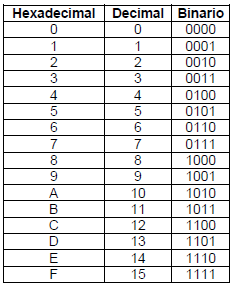
\includegraphics[width=0.5\linewidth]{Art/art1.png}
\caption{Equivalencias entre binario, decimal y hexadecimal.}
\label{fig: bin a hex}
\end{figure}
\begin{example}[Convertir $1010110101_2$ a hexadecimal]
Primero debemos de agrupar en grupos de 4 bits:\\
0010 1011 0101\\
Ahora usando la figura \ref{fig: bin a hex}, buscamos sus equivalentes:
\begin{displaymath}
0010 1011 0101_2=2B5_{16}
\end{displaymath}
\end{example}
\subsection{Hexadecimal a binario}
Aquí resulta lo mismo, cada letra y número del sistema hexadecimal lo cambiamos a binario usando la figura \ref{fig: bin a hex}. Recordar que cada letra y número representa 4 bits. No hay más ciencia detrás de esto.
\subsection{Hexadecimal a decimal}
Se usa el mismo recurso de suma de potencias, solo que son base de 16 por la unidad, recordando los valores de la figura \ref{fig: bin a hex}.
\begin{example}[Pasar $2BAF_{16}$ a decimal]
Multiplicamos cada número por la potencia de 16 correspondiente vista antes:
\begin{displaymath}
2\cdot 16^3 + B\cdot 16^2 + A\cdot 16^1 + F\cdot 16^0
\end{displaymath}
Así no podemos operar debido a las letras, reemplazando sus valores de \ref{fig: bin a hex}:
\begin{displaymath}
2\cdot 16^3 + 11\cdot 16^2 + 10\cdot 16^1 + 15\cdot 16^0=11 183_{10}
\end{displaymath}
\end{example}
\subsection{Decimal a hexadecimal}
Este es probablemente el más trabajoso, una manera fácil es tener al sistema binario como intermediario, es decir: pasamos de decimal a binario y de binario a hexadecimal.\\
Si no hacemos eso tenemos otra forma que son divisiones sucesivas al número en base 10 entre 16, hasta que cociente sea 1. Una vez que lleguemos ahí, tomamos los residuos de derecha a izquierda, y los escribimos nosotros de izquierda a derecha. Los números 10, 11, 12, 13, 14 y 15 los reemplazamos por sus letras correspondiente.
\newcount\total
\newcount\lasttotal
\newcount\targetbase

\def\basetenconversiontable#1#2{%
    \begin{tikzpicture}[every node/.style={minimum width=1cm, minimum height=0.5cm}, x=1cm,y=0.5cm]
    %
    \total=#1%
    \targetbase=#2
    \def\newnumber{}
    %
    \pgfmathloop
    \ifnum\total<1
    \else
        %
        \ifnum\pgfmathcounter>1
            \node at (\pgfmathcounter, -\pgfmathcounter+1) (tmp) {\the\targetbase};
            \draw (tmp.north west) |- (tmp.south east);
            %
            \node at (\pgfmathcounter-1, -\pgfmathcounter) (tmp) {\pgfmathparse{int(\total*\targetbase)}\pgfmathresult};
            \draw (tmp.south west) -- (tmp.south east);
            %
            \pgfmathparse{int(\lasttotal-\total*\targetbase)}%
            \let\digit=\pgfmathresult
            \node at (\pgfmathcounter-1, -\pgfmathcounter-1) [text=red] {\digit};
            \edef\newnumber{\digit\newnumber}
        \fi
        %
        \ifnum\total<\targetbase
                \edef\newnumber{\the\total\newnumber}
            \node at (\pgfmathcounter, -\pgfmathcounter) [text=red]  {\the\total};
        \else
            \node at (\pgfmathcounter, -\pgfmathcounter) {\the\total};
        \fi
        \lasttotal=\total
        \divide\total by\targetbase
    \repeatpgfmathloop    
    \draw [->] (\pgfmathcounter-1,-\pgfmathcounter-1) -- ++(-0.5,0); 
    \node [anchor=west] at (1, -\pgfmathcounter-2) {$#1=\newnumber_{\the\targetbase}$};
    \end{tikzpicture}   
}
\begin{example}[Pasar $478_{10}$ a sistema hexadecimal]
Lo único que hacemos es dividir y dividir entre 16, hasta que el cociente sea 1, ten en cuenta que los residuos pues nos interesan:
\begin{center}
\begin{tabular}{c}
\basetenconversiontable{478}{16}
\end{tabular}
\end{center}
Ya tenemos los residuos, ahora identifica los residuos que no son permitidos en esta base, en otras palabras, reemplaza los números 10, 11, 12, 13, 14 y 15 por sus letras:\\
1\textcolor{red}{13}\textcolor{blue}{14}=$1\textcolor{red}{D}\textcolor{blue}{E}_{16}$
\end{example}
\chapterimage{chapter_head_SD.pdf} % Chapter heading image
\chapter{Lógica digital}
Un sistema digital binario es un conjunto de dispositivos que son destinados a la generación, transmisión, manejo, procesamiento y almacenamiento de señales digitales.
\section{Compuertas lógicas}\index{Compuertas lógicas}
\subsection{Compuerta NOT}
\begin{figure}[H]
\centering
\subfloat[Estilo Americano]{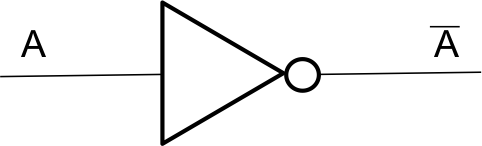
\includegraphics[scale=0.8]{SD/SD1.png}}
\subfloat[Estilo Europeo]{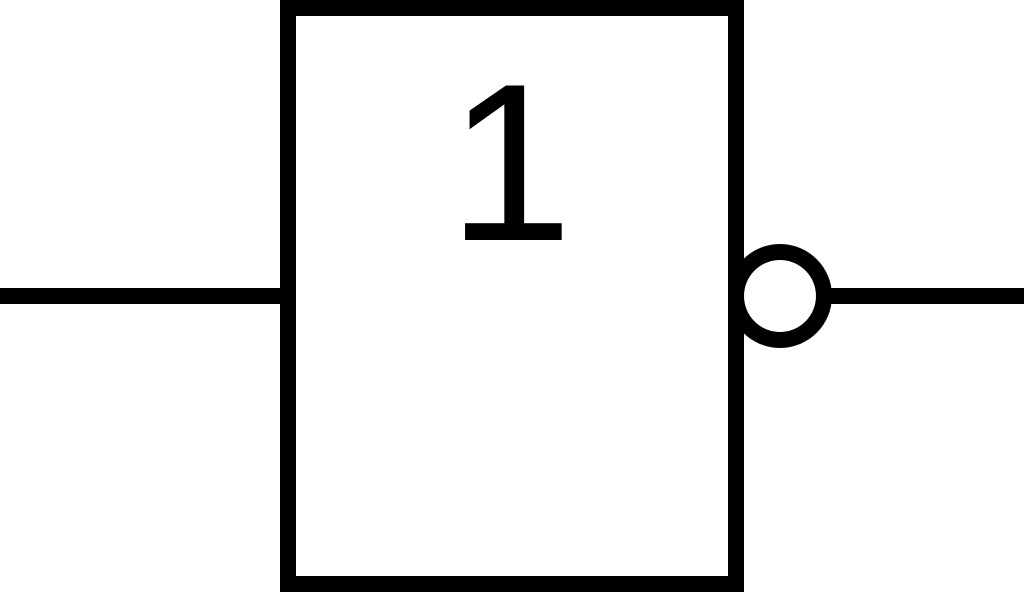
\includegraphics[scale=0.1]{SD/SD2.png}}
\caption{Simbología compuerta NOT}
\end{figure}
\begin{figure}[h!]
\centering
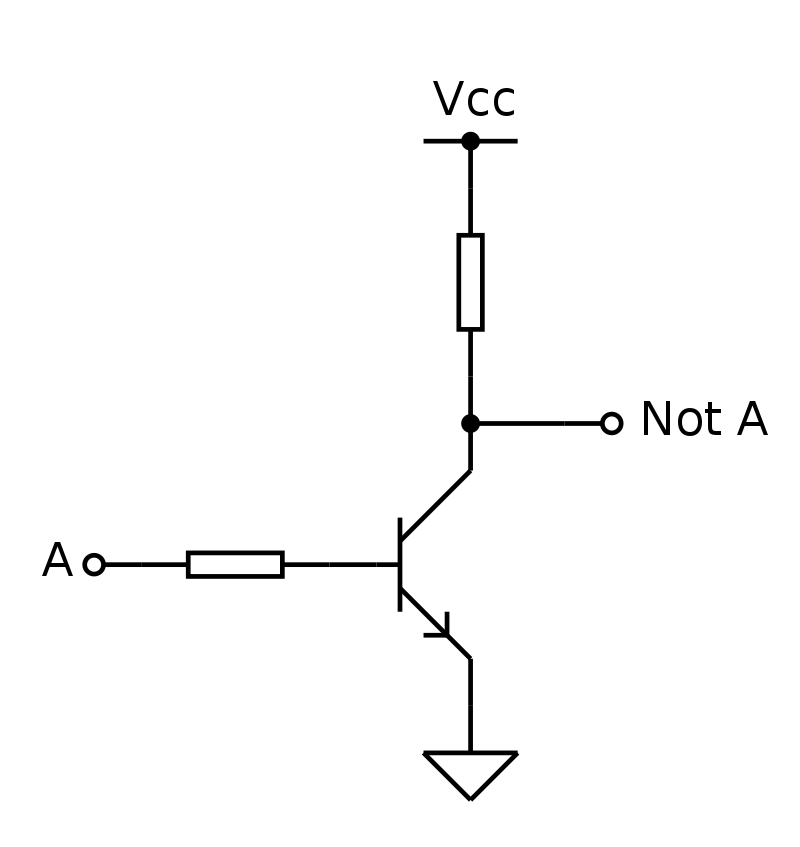
\includegraphics[scale=0.15]{SD/SD3.png}
\caption{Implementación electrónica: Compuerta NOT}
\end{figure}
\begin{table}[H]
\begin{center}
\begin{tabular}{|c|c|}
\hline
\rowcolor{color1}
IN & OUT \\ \hline
0  & 1   \\ \hline
1  & 0   \\ \hline
\end{tabular}
\end{center}
\caption{Tabla de verdad de la compuerta NOT}
\label{table:nottable}
\end{table}

\subsection{Compuerta AND}
\begin{figure}[H]
\centering
\subfloat[Estilo Americano]{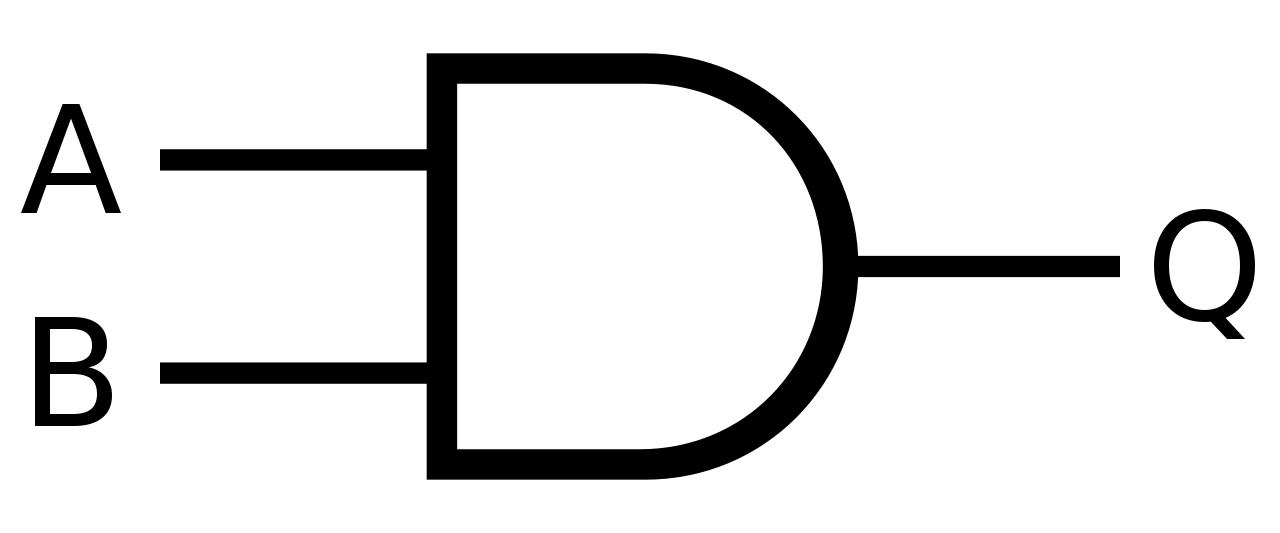
\includegraphics[scale=0.1]{SD/SD4.png}}
\subfloat[Estilo Europeo]{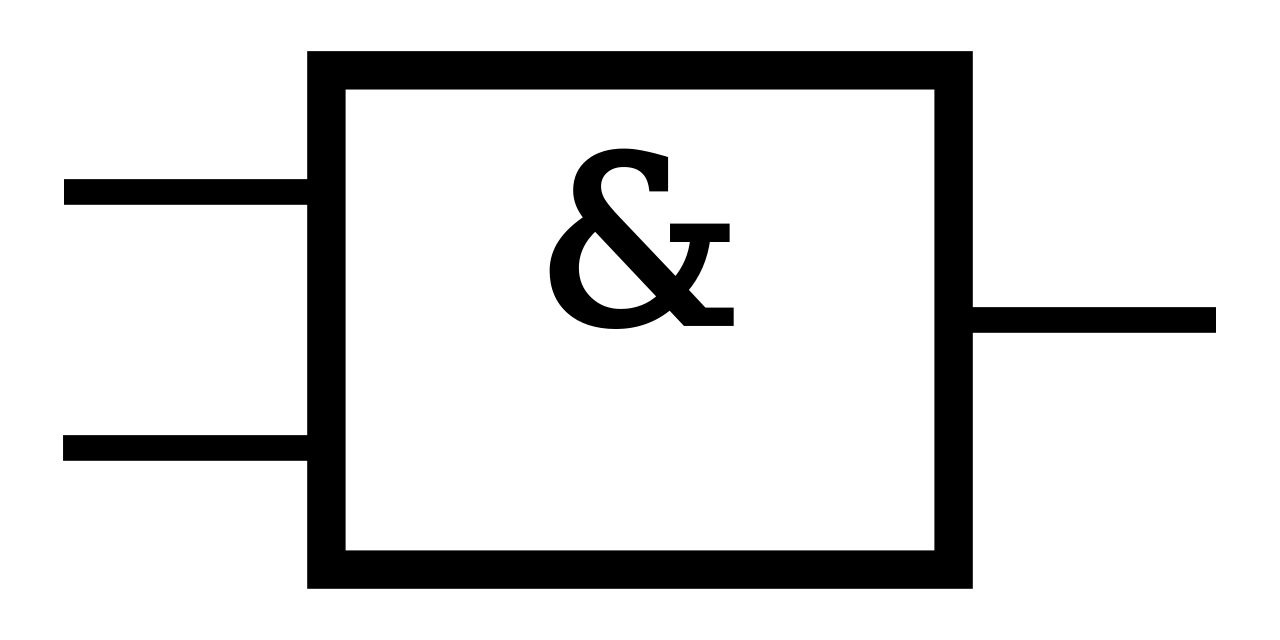
\includegraphics[scale=0.1]{SD/SD5.png}}
\caption{Simbología compuerta AND}
\end{figure}
\begin{figure}[H]
\centering
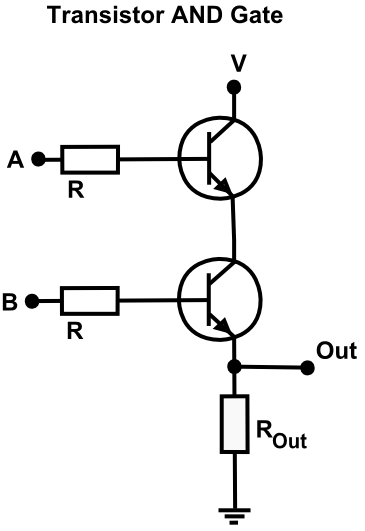
\includegraphics[scale=0.5]{SD/SD6.png}
\caption{Implementación electrónica: Compuerta AND}
\end{figure}
\begin{table}[H]
\begin{center}
\begin{tabular}{|cc|c|}
\hline
\rowcolor{color1}
\multicolumn{2}{|c|}{IN}    & OUT \\ \hline
\rowcolor{color1!70}
\multicolumn{1}{|c|}{A} & B & Q   \\ \hline
\multicolumn{1}{|c|}{0} & 0 & 0   \\ \hline
\multicolumn{1}{|c|}{0} & 1 & 0   \\ \hline
\multicolumn{1}{|c|}{1} & 0 & 0   \\ \hline
\multicolumn{1}{|c|}{1} & 1 & 1   \\ \hline
\end{tabular}
\end{center}
\caption{Tabla de verdad de la compuerta AND}
\label{table:andtable}
\end{table}
Se puede caracterizar como:
\begin{displaymath}
A\times B\times C\times \cdots = X
\end{displaymath}
La salida será 1 solo si todas las entradas son 1.
\subsection{Compuerta OR}
\begin{figure}[H]
\centering
\subfloat[Estilo Americano]{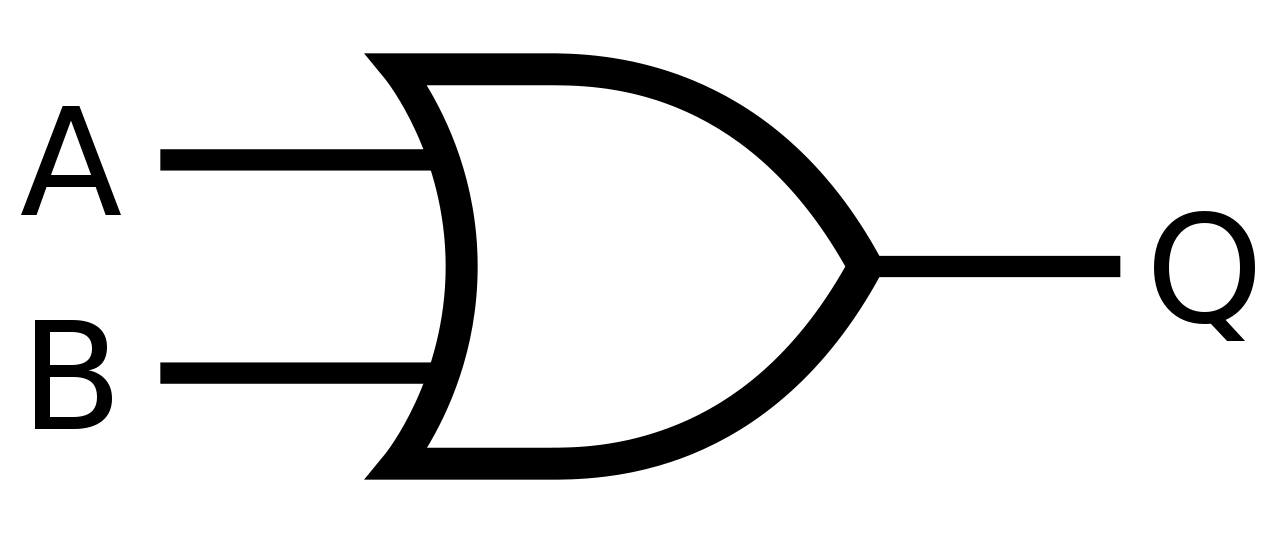
\includegraphics[scale=0.1]{SD/SD7.png}}
\subfloat[Estilo Europeo]{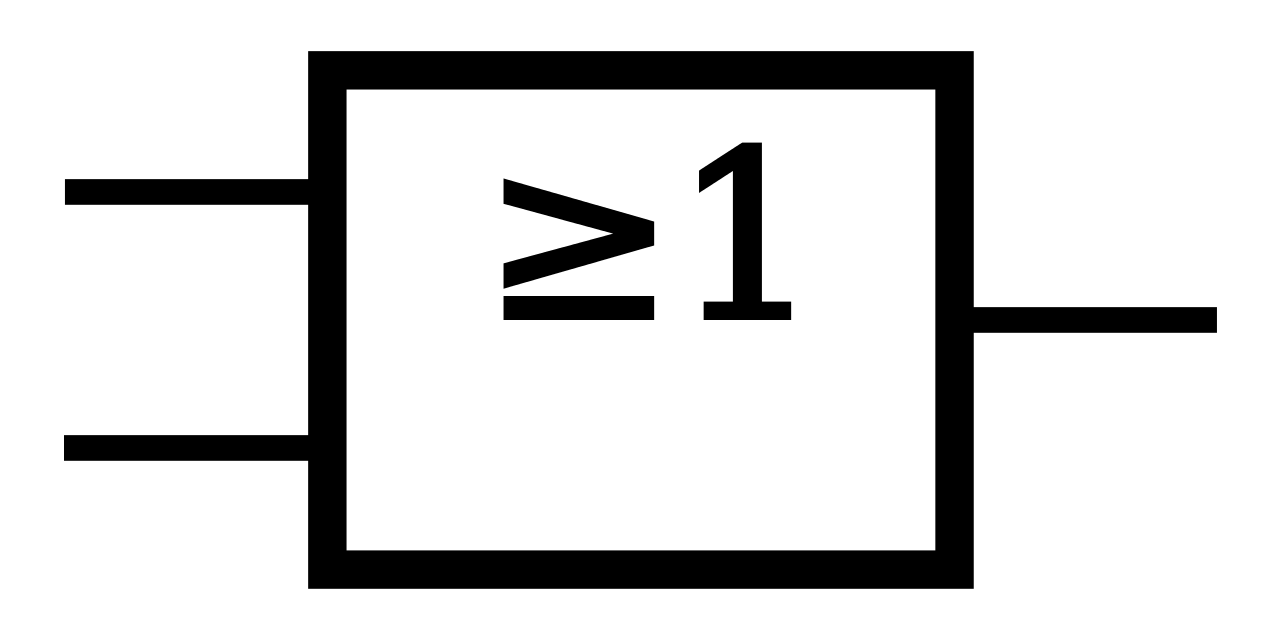
\includegraphics[scale=0.1]{SD/SD8.png}}
\caption{Simbología compuerta OR}
\end{figure}
\begin{figure}[H]
\centering
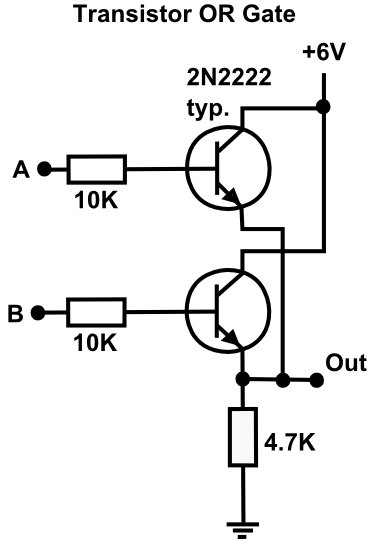
\includegraphics[scale=0.5]{SD/SD9.png}
\caption{Implementación electrónica: Compuerta OR}
\end{figure}
\begin{table}[H]
\begin{center}
\begin{tabular}{|cc|c|}
\hline
\rowcolor{color1}
\multicolumn{2}{|c|}{IN}    & OUT \\ \hline
\rowcolor{color1!70}
\multicolumn{1}{|c|}{A} & B & Q   \\ \hline
\multicolumn{1}{|c|}{0} & 0 & 0   \\ \hline
\multicolumn{1}{|c|}{0} & 1 & 1   \\ \hline
\multicolumn{1}{|c|}{1} & 0 & 1   \\ \hline
\multicolumn{1}{|c|}{1} & 1 & 1   \\ \hline
\end{tabular}
\end{center}
\caption{Tabla de verdad de la compuerta OR}
\label{table:ortable}
\end{table}
\begin{displaymath}
A + B + C + \cdots = X
\end{displaymath}
La salida será 0 solo si todas las entradas son 0.
\pagebreak
\subsection{Compuerta NAND}
Solo cuando todas sus entradas son ALTO, la salida será BAJO.
\begin{figure}[H]
\centering
\subfloat[Estilo Americano]{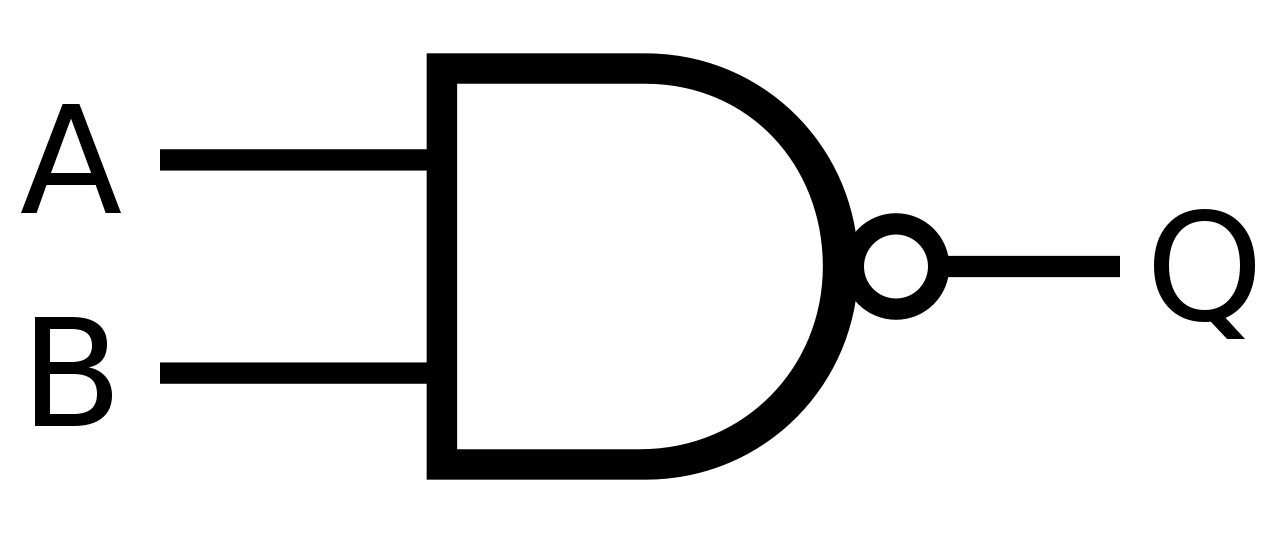
\includegraphics[scale=0.1]{SD/SD10.png}}
\subfloat[Estilo Europeo]{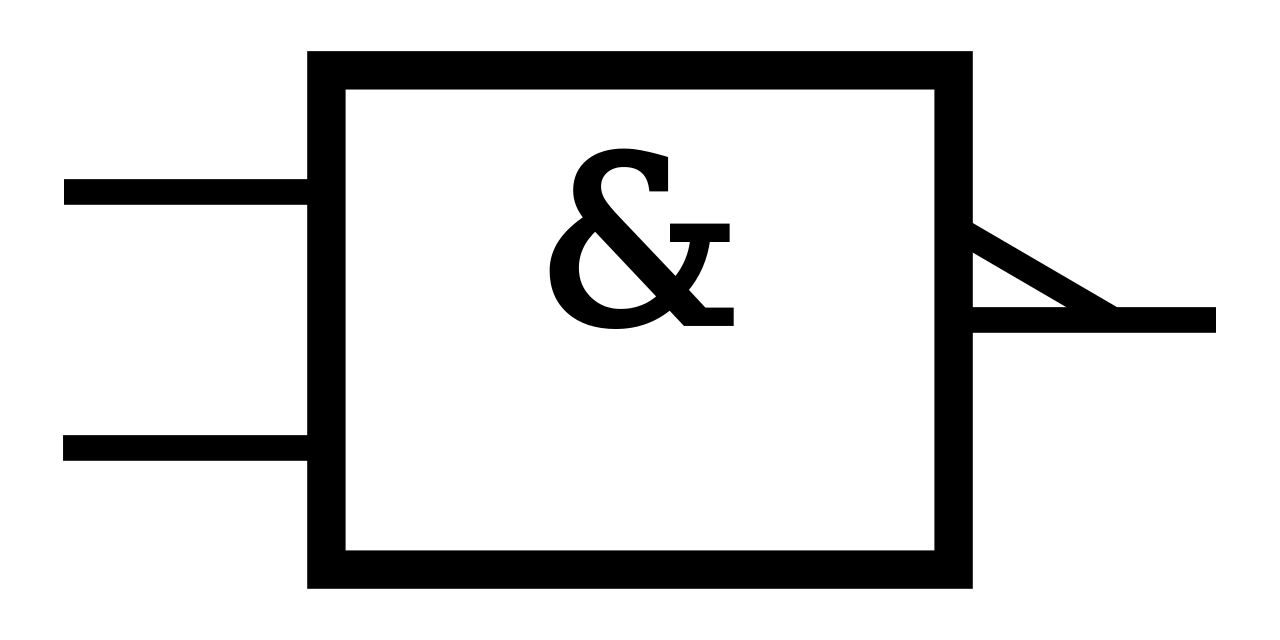
\includegraphics[scale=0.1]{SD/SD11.png}}
\caption{Simbología compuerta NAND}
\end{figure}
\begin{figure}[H]
\centering
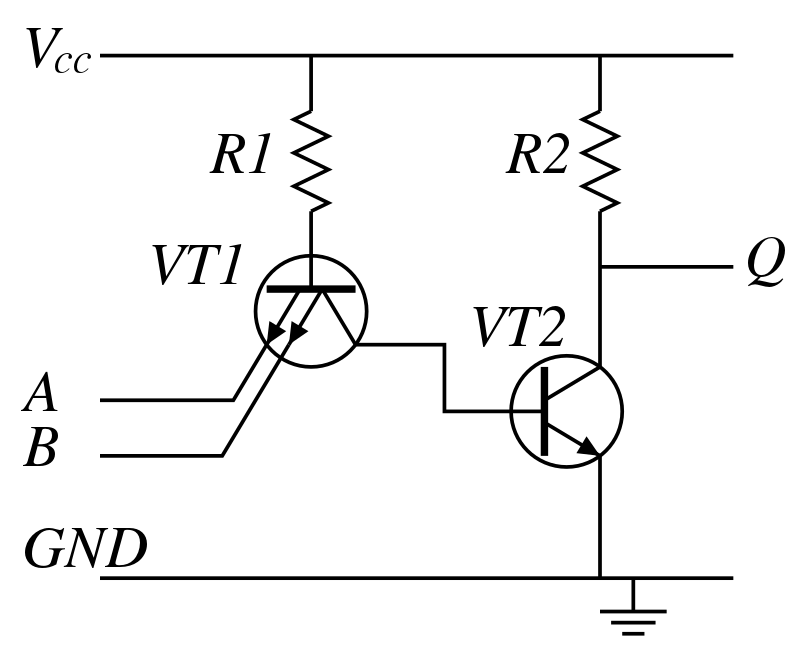
\includegraphics[scale=0.3]{SD/SD12.png}
\caption{Implementación electrónica: Compuerta NAND}
\end{figure}
\begin{table}[H]
\begin{center}
\begin{tabular}{|cc|c|}
\hline
\rowcolor{color1}
\multicolumn{2}{|c|}{IN}    & OUT \\ \hline
\rowcolor{color1!70}
\multicolumn{1}{|c|}{A} & B & Q   \\ \hline
\multicolumn{1}{|c|}{0} & 0 & 1   \\ \hline
\multicolumn{1}{|c|}{0} & 1 & 1   \\ \hline
\multicolumn{1}{|c|}{1} & 0 & 1   \\ \hline
\multicolumn{1}{|c|}{1} & 1 & 0   \\ \hline
\end{tabular}
\end{center}
\caption{Tabla de verdad de la compuerta NAND}
\label{table:nandtable}
\end{table}
%Solo si todas las entradas son 1 la salida es 0.
%Otra forma de expresar es negando la salida de la compuerta AND:
%\begin{table}[H]
%\begin{tabular}{|c|c|c|}
%\hline
%A & B & \bar{AB} = X                                                                          \\ \hline
%0 & 0 & \bar{0$\cdot$ 0} \rightarrow \bar{0} = 1 \\ \hline
%0 & 1 & \bar{0$\cdot$ 1} \rightarrow \bar{0} = 1 \\ \hline
%1 & 0 & \bar{1$\cdot$ 0} \rightarrow \bar{0} = 1 \\ \hline
%1 & 1 & \bar{1$\cdot$ 1} \rightarrow \bar{1} = 0 \\ \hline
%\end{tabular}
%\end{table}
\pagebreak
\subsection{Compuerta NOR}
\begin{figure}[H]
\centering
\subfloat[Estilo Americano]{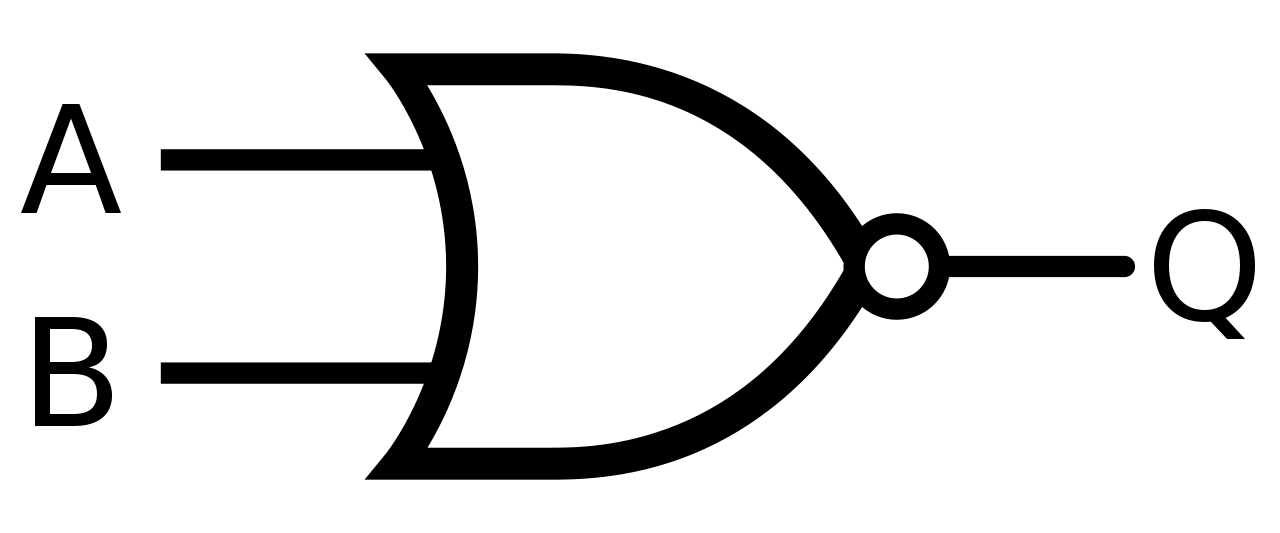
\includegraphics[scale=0.1]{SD/SD13.png}}
\subfloat[Estilo Europeo]{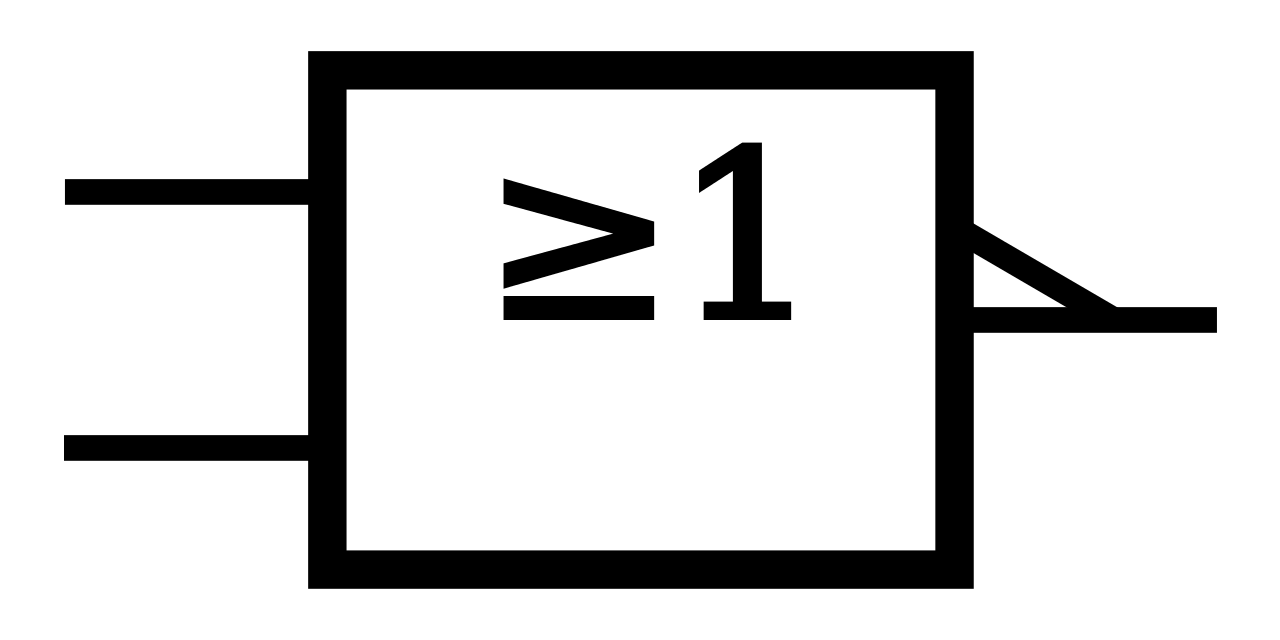
\includegraphics[scale=0.1]{SD/SD14.png}}
\caption{Simbología compuerta NOR}
\end{figure}
\begin{figure}[H]
\centering
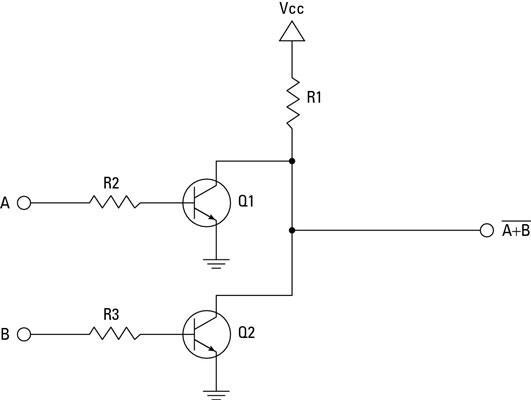
\includegraphics[scale=0.5]{SD/SD15.png}
\caption{Implementación electrónica: Compuerta NOR}
\end{figure}
\begin{table}[H]
\begin{center}
\begin{tabular}{|cc|c|}
\hline
\rowcolor{color1}
\multicolumn{2}{|c|}{IN}    & OUT \\ \hline
\rowcolor{color1!70}
\multicolumn{1}{|c|}{A} & B & Q   \\ \hline
\multicolumn{1}{|c|}{0} & 0 & 1   \\ \hline
\multicolumn{1}{|c|}{0} & 1 & 0   \\ \hline
\multicolumn{1}{|c|}{1} & 0 & 0   \\ \hline
\multicolumn{1}{|c|}{1} & 1 & 0   \\ \hline
\end{tabular}
\end{center}
\caption{Tabla de verdad de la compuerta NOR}
\label{table:nortable}
\end{table}
Solo si todas las entradas son 0, la salida será 1.
\pagebreak
\subsection{Compuerta OR exclusiva-XOR}
\begin{figure}[H]
\centering
\subfloat[Estilo Americano]{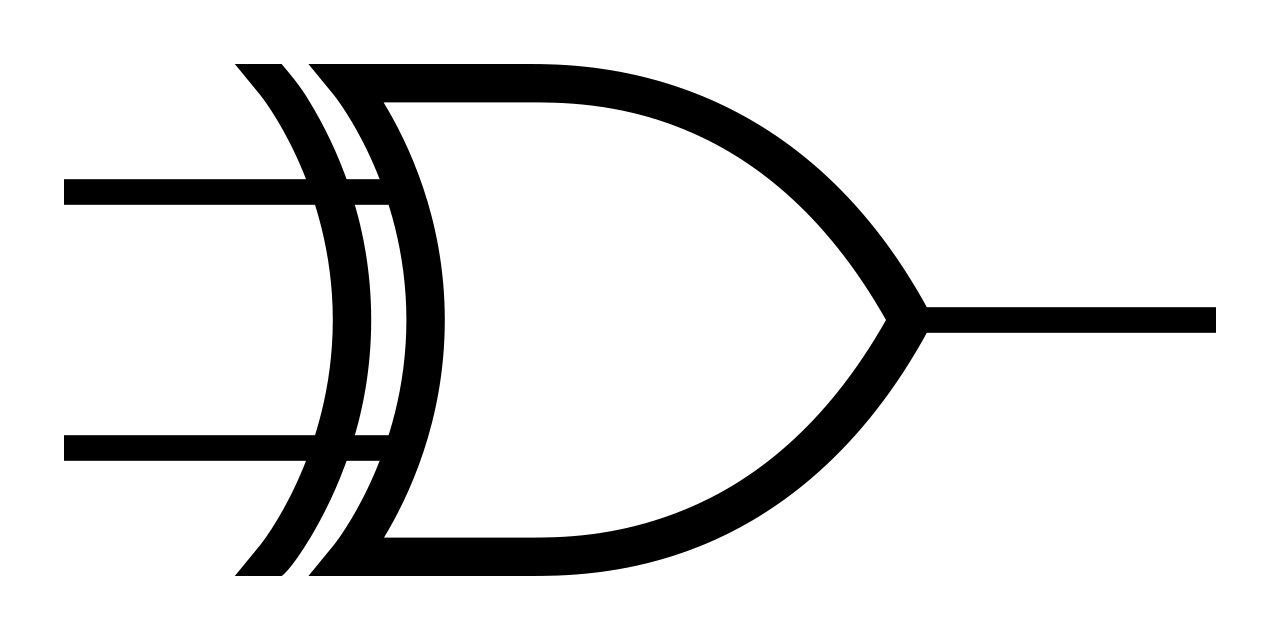
\includegraphics[scale=0.1]{SD/SD16.png}}
\subfloat[Estilo Europeo]{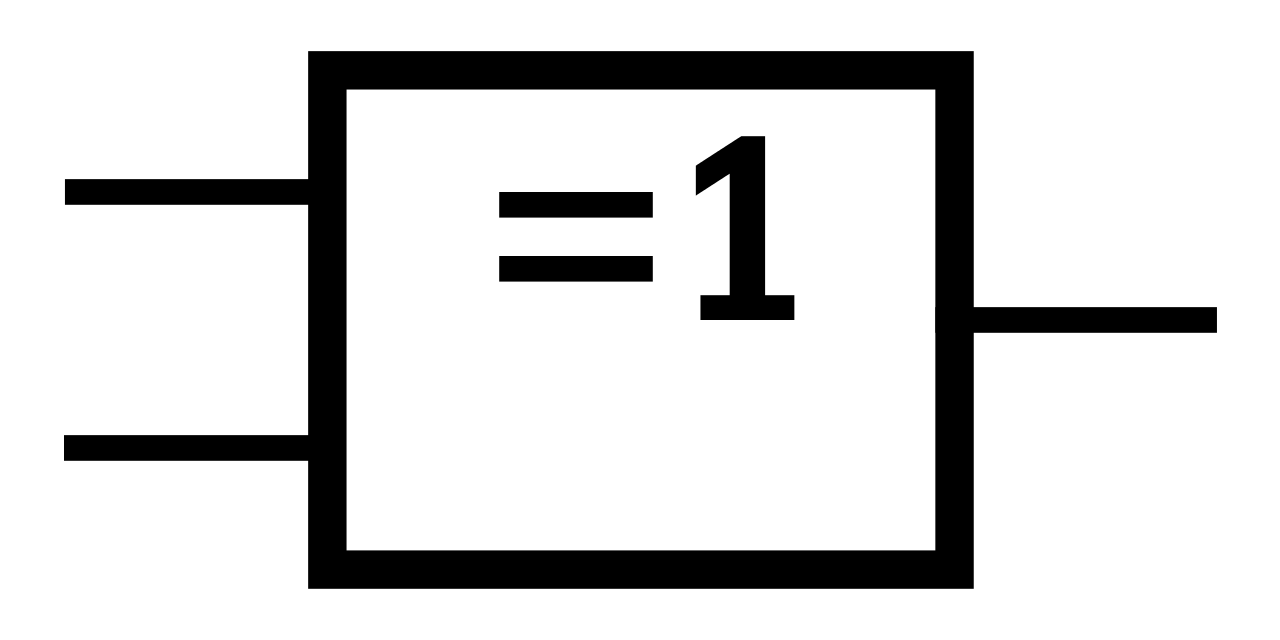
\includegraphics[scale=0.1]{SD/SD17.png}}
\caption{Simbología compuerta XOR}
\end{figure}
\begin{figure}[H]
\centering
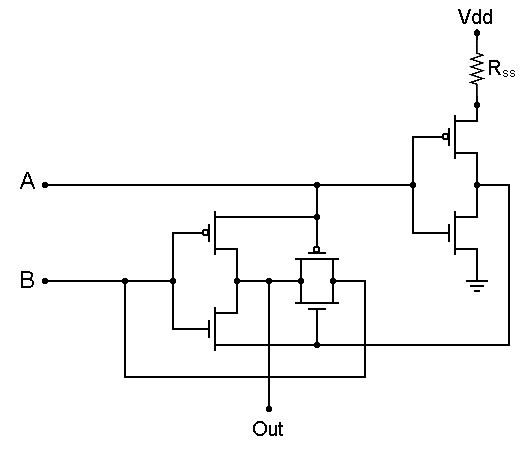
\includegraphics[scale=0.5]{SD/SD18.png}
\caption{Implementación electrónica: Compuerta XOR}
\end{figure}
\begin{table}[H]
\begin{center}
\begin{tabular}{|cc|c|}
\hline
\rowcolor{color1}
\multicolumn{2}{|c|}{IN}    & OUT \\ \hline
\rowcolor{color1!70}
\multicolumn{1}{|c|}{A} & B & Q   \\ \hline
\multicolumn{1}{|c|}{0} & 0 & 0   \\ \hline
\multicolumn{1}{|c|}{0} & 1 & 1   \\ \hline
\multicolumn{1}{|c|}{1} & 0 & 1   \\ \hline
\multicolumn{1}{|c|}{1} & 1 & 0   \\ \hline
\end{tabular}
\end{center}
\caption{Tabla de verdad de la compuerta XOR}
\label{table:xortable}
\end{table}
\pagebreak
\subsection{Compuerta NOR exclusiva-XNOR}
\begin{figure}[H]
\centering
\subfloat[Estilo Americano]{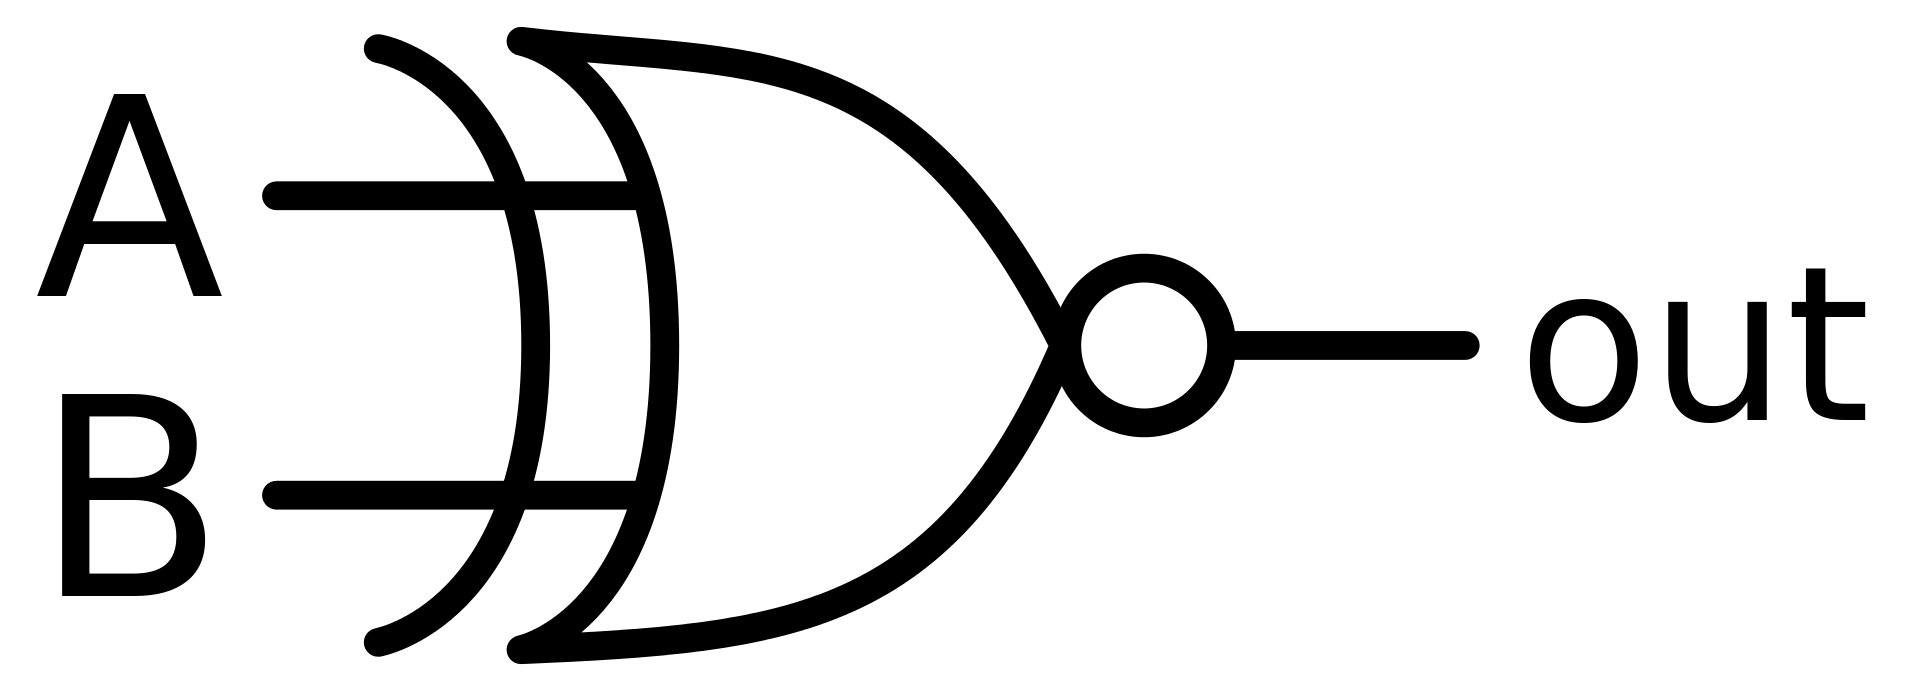
\includegraphics[scale=0.1]{SD/SD19.png}}
\subfloat[Estilo Europeo]{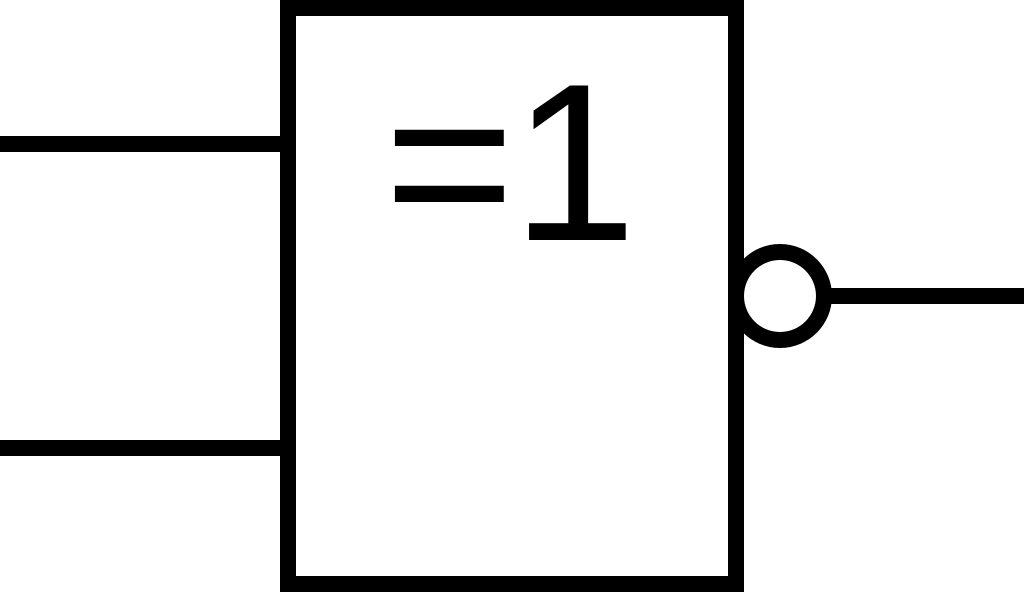
\includegraphics[scale=0.1]{SD/SD20.png}}
\caption{Simbología compuerta XNOR}
\end{figure}
\begin{figure}[H]
\centering
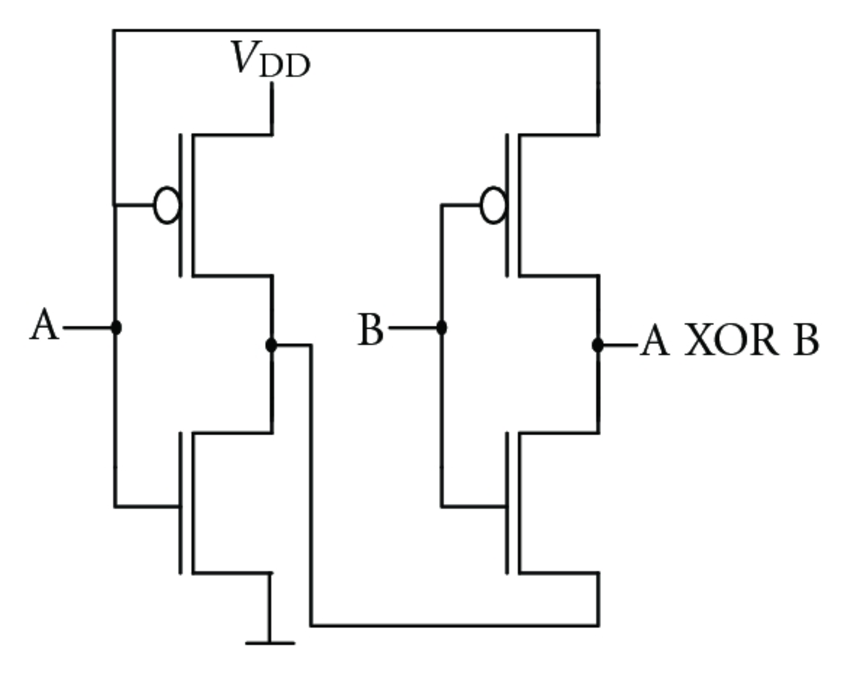
\includegraphics[scale=0.8]{SD/SD21.png}
\caption{Implementación electrónica: Compuerta XNOR}
\end{figure}
\begin{table}[H]
\begin{center}
\begin{tabular}{|cc|c|}
\hline
\rowcolor{color1}
\multicolumn{2}{|c|}{IN}    & OUT \\ \hline
\rowcolor{color1!70}
\multicolumn{1}{|c|}{A} & B & Q   \\ \hline
\multicolumn{1}{|c|}{0} & 0 & 1   \\ \hline
\multicolumn{1}{|c|}{0} & 1 & 0   \\ \hline
\multicolumn{1}{|c|}{1} & 0 & 0   \\ \hline
\multicolumn{1}{|c|}{1} & 1 & 1   \\ \hline
\end{tabular}
\end{center}
\caption{Tabla de verdad de la compuerta XNOR}
\label{table:xnortable}
\end{table}
\section{Formas de expresar funciones booleanas}\index{Formas de expresar funciones booleanas}
Existen formas de expresar las funciones booleanas: como \textbf{suma de productos} o como \textbf{productos de sumas.}
\subsection{Suma de productos-SOP}
Suma(\textbf{OR}) de términos(\textbf{AND}), formados por varias variables complementadas o no. Aqui nos importan las salidas con nivel \textbf{ALTO}. Como entradas, un nivel alto será A=1 mientras que un nivel bajo es A'=0.
\begin{displaymath}
f(a,b,c)=\bar{a}bc+a\bar{b}\bar{c}+abc+c
\end{displaymath}
\subsection{Productos de sumas-POS}
Productos(\textbf{AND}) de sumas(\textbf{OR}) formadas por varias variables complementadas o no. Aqui nos importan las salidas con nivel \textbf{BAJO}. Como entradas, un nivel alto será A'=1 mientras que un nivel bajo es A=0.
\begin{displaymath}
F(a,b,c)=(A+B+C)(A+B'+C')(C'+A)
\end{displaymath}
\begin{remark}
La terminología de la negación puede tener varias formas, en este libro usaremos dos: \textbf{$\bar{A}$} o A'. Ambos significan lo mismo. Asimismo, para el POS usaré letras mayúsculas y para SOP usaré letras minúsculas. Lo más importante es que entiendas como funciona todo así la terminología no será un problema.
\end{remark}
Se detallará un ejemplo para poder explicar los SOP y POS para 3 variables. La tabla puede ser expandida para más variables pero todo funcionará bajo la misma lógica.
\begin{table}[h]
\begin{tabular}{|c|c|c|c|c|c|c|c|}
\hline
\rowcolor{color1}
F & A & B & C & Min término & Notación minterm & Max término & Notación maxterm \\ \hline
0 & 0 & 0 & 0 & A'B'C'      & $m_0$               & A+B+C       & $M_0$               \\
1 & 0 & 0 & 1 & A'B'C       & $m_1$               & A+B+C'      & $M_1$               \\
2 & 0 & 1 & 0 & A'BC'       & $m_2$               & A+B'+C      & $M_2$               \\
3 & 0 & 1 & 1 & A'BC        & $m_3$               & A+B'+C'     & $M_3$               \\
4 & 1 & 0 & 0 & AB'C'       & $m_4$               & A'+B+C      & $M_4$               \\
5 & 1 & 0 & 1 & AB'C        & $m_5$               & A'+B+C'     & $M_5$               \\
6 & 1 & 1 & 0 & ABC'        & $m_6$               & A'+B'+C     & $M_6$               \\
7 & 1 & 1 & 1 & ABC         & $m_7$               & A'+B'+C'    & $M_7$               \\ \hline
\end{tabular}
\caption{Notación de \textit{minterm} y \textit{maxterm}.}
\label{tab:maxmin}
\end{table}
\begin{example}
Se presenta la tabla \ref{tab:ejemplo1}, expresar la misma tabla como SOP y como POS.\\
\textbf{SOP:}\\
En SOP, solo nos fijamos en las salidas de nivel ALTO(1). Una vez que las hayamos ubicado escribimos las filas tal y como están expresando las entradas como un producto. Por ejemplo, el primer ALTO se encuentra en la posición de $F_1$, donde A y B son nivel BAJO y C es nivel ALTO. Escribimos, según la teoría, donde ALTO es A y BAJO es A', el primer sumando como: A'B'C. Repetimos el mismo paso para $F_3$, $F_4$, $F_5$, $F_6$ y $F_7$ puesto que tienen un nivel ALTO como salida. Si seguimos la bajo la lógica que se vio y sumando cada sumando obtendremos:
\begin{displaymath}
f(a,b,c)=\underbrace{A'B'C}_{F_1}+\underbrace{A'BC}_{F_3}+\underbrace{AB'C}_{F_5}+\underbrace{ABC'}_{F_6}+\underbrace{ABC}_{F_7}
\end{displaymath}
Esta expresión también puede ser reducida usando notación dicha en la tabla \ref{tab:maxmin}. Como la tabla y nuestro ejemplo son de 3 variables de entrada, solo buscamos la equivalencia dentro de la columna \textit{Notación minterm}, la forma reducida sería:
\begin{displaymath}
f(a,b,c)=m_1+m_3+m_5+m_6+m_7
\end{displaymath}
\textbf{POS:}\\
Para POS, en vez de fijarnos en los niveles ALTOS, nos fijamos en los niveles BAJOS y seguimos la misma lógica vista en SOP, sin embargo, ahora en vez de cada fila sea expresada como un producto y luego sumemos todos, en este caso cada fila se expresa como una suma, y al agrupar todos los términos será mediante una suma. Así, los ceros están en las ubicaciones $F_0$, $F_2$ y $F_4$, entonces, según la teoría 1 será A' y 0 será A:
\begin{displaymath}
F(A,B,C)=\underbrace{(A+B+C)}_{F_0}\cdot\underbrace{(A+B'+C)}_{F_2}\cdot\underbrace{(A'+B+C)}_{F_4}
\end{displaymath}
Según la tabla \ref{tab:maxmin} también puede ser simplificado:
\begin{displaymath}
F(A,B,C)=M_0M_2M_5
\end{displaymath}
\end{example}
\begin{table}[h]
\centering
\begin{tabular}{c|ccc|c}
\rowcolor{color1}
$F_1$ & A & B & C & F \\ \hline
0   & 0 & 0 & 0 & 0 \\
1   & 0 & 0 & 1 & 1 \\
2   & 0 & 1 & 0 & 0 \\
3   & 0 & 1 & 1 & 1 \\
4   & 1 & 0 & 0 & 0 \\
5   & 1 & 0 & 1 & 1 \\
6   & 1 & 1 & 0 & 1 \\
7   & 1 & 1 & 1 & 1
\end{tabular}
\caption{Tabla ejemplo 1}
\label{tab:ejemplo1}
\end{table}
\subsection{Conversión de SOP a POS}
A veces es necesario expresar de una forma u otra, es por eso que usa la conversión de SOP a POS. Se explicará usando un ejemplo:
\begin{displaymath}
f(x,y,z)=x'y'z'+x'yz+x'yz'+xy'z
\end{displaymath}
\begin{enumerate}
\item Evaluamos los binarios de los sumando, recordando las equivalencias:
\begin{displaymath}
f(x,y,z)=\underbrace{\underbrace{x'y'z'}_{\textcolor{red}{000}}}_{\textcolor{blue}{0}}+\underbrace{\underbrace{x'yz}_{\textcolor{red}{011}}}_{\textcolor{blue}{3}}+\underbrace{\underbrace{x'y'z'}_{\textcolor{red}{010}}}_{\textcolor{blue}{2}}+\underbrace{\underbrace{x'y'z'}_{\textcolor{red}{101}}}_{\textcolor{blue}{5}}
\end{displaymath}
El color rojo es su equivalente en binario mientras que el azul lo es en decimal.\\
\item Identificamos los términos faltantes, como es una función lógica de 3 variables: $2^3=8$, en el paso uso, con la ayuda de nuestra tabla \ref{tab:maxmin} logramos identificar a los términos 0,3,2,5; por consecuente nos faltan los términos 1, 4, 6 y 7 cuyos binarios son:
\begin{itemize}
\item 1=001
\item 4=100
\item 6=110
\item 7=111
\end{itemize}
\item Ahora escribimos esos mismos términos que faltan(1, 4, 6 y 7) como POS:
\begin{displaymath}
f(a,b,c)=\underbrace{(A+B+C')}_{\textcolor{blue}{1}}\cdot\underbrace{(A'+B+C)}_{\textcolor{blue}{4}}\cdot\underbrace{(A'+B'+C)}_{\textcolor{blue}{6}}\cdot\underbrace{(A'+B'+C')}_{\textcolor{blue}{7}}
\end{displaymath}
\end{enumerate}
\subsection{Forma canónica}
Función en donde cada sumando o multiplicando aparecen todas las entradas, sin importar si están negada o no; en otras palabras, si se tiene una función de tres variables $f(a,b,c)$, una expresión canónica puede ser:
\begin{displaymath}
f(a,b,c)=ab'c+a'b'c+abc+a'b'c'
\end{displaymath}
\subsection{Forma normalizada}
Reducción de la forma canónica mediante el álgebra de conmutación. De tener, por ejemplo, una función $f(a,b,c)$, una forma normalizada sería:
\begin{displaymath}
f(a,b,c)=a+bc'+a'c
\end{displaymath}
Vemos que en cada sumando o producto no estan presente todas las variables.
\subsection{¿Cómo pasar de la forma normalizara a la canónica?}
\begin{enumerate}
\item \textbf{Identificar} los sumandos de \textbf{NO} estén completos, usaremos de ejemplo la siguiente función lógica: $f(a,b,c)=a+bc+\overline{abc}$\footnote{Otra manera de expresar la negación aparte de $\overline{A}$, A' es /A}
\begin{displaymath}
f(a,b,c)=\textcolor{red}{a}+\textcolor{red}{bc}+\textcolor{blue}{\overline{abc}}
\end{displaymath}
Los términos en color \textcolor{red}{rojo} son los términos que están incompletos, es decir, no están presentes todas las variables a excepción del tercer sumando de \textcolor{blue}{azul}.
\item \textbf{Completar} los términos incompletos. Aunque haya una teoría detrás de todo, lo más rápido es completar los términos incompletos con todas las variaciones posibles. En este caso tenemos 3 variables, así que procedemos:
\begin{itemize}
\item \textbf{a}:En el caso de tener un solo término, en nuestro ejemplo \textit{a}, sabemos que a este sumando le faltan 2 variables: b y c. Entonces repetimos el término unitario(\textit{a} en nuestro caso) \textbf{$2^n$ veces}, donde n es el número de variables faltantes; en este caso es n=2 porque falta b y c. Una vez que hayamos repetidos $2^n$ veces la variable unitaria, a cada una de ellas escribimos las posibles combinaciones que pueden tomar las dos variables restantes:
\begin{align*}
&\textcolor{red}{a}\hspace{20pt}\textcolor{violet}{\overline{b}}\hspace{20pt}\textcolor{magenta}{\overline{c}}\\
&\textcolor{red}{a}\hspace{20pt}\textcolor{violet}{\overline{b}}\hspace{20pt}\textcolor{magenta}{c}\\
&\textcolor{red}{a}\hspace{20pt}\textcolor{violet}{b}\hspace{20pt}\textcolor{magenta}{\overline{c}}\\
&\textcolor{red}{a}\hspace{20pt}\textcolor{violet}{b}\hspace{20pt}\textcolor{magenta}{c}\\
\end{align*}
Hemos generado 4 términos.
\item \textbf{bc}: Repetimos el mismo paso anterior, ahora \textit{n} será 1, por lo tanto $2^n=2$, repetimos dos veces el término \textit{bc} y completamos con las posibles variantes del término faltante:
\begin{align*}
&\textcolor{red}{b\hspace{20pt}c}\hspace{20pt}\textcolor{violet}{\overline{a}}\\
&\textcolor{red}{b\hspace{20pt}c}\hspace{20pt}\textcolor{violet}{a}\\
\end{align*}
Hemos generado 2 términos.
\end{itemize}
El procedimiento será el mismo para más variables, sin embargo para más variables será más largo el proceso. 
\item \textbf{Sumamos} todos los términos hallados, incluso los que no hemos tocado ($\overline{abc}$), al sumarlos todos debemos tener el cuenta el teorema \ref{theo:potenciasidenticas}, en otras palabras, términos repetidos solo se colocan una vez.
\end{enumerate}
\begin{remark}
Es común que escuchemos diferentes formas de expresar un circuito lógico. Una común es expresión booleana: Esta es una forma de expresar la salida como las operaciones que se realizan. Por ejemplo, sean las entradas A y B, la salida de una compuerta AND es A$\cdot$ B, la compuerta OR se expresa como A+B, la compuerta XOR $\oplus$ y así existen otros operadores para las demás compuerta y circuitos lógicos.
\end{remark}
\section{Axiomas}\index{Axiomas}
Los axiomas los conjuntos minimos de definiciones básicas que suponemos como verdaderas:
\begin{enumerate}
\item X=0 si X$\neq$1 $\lor$ X=1 si X$\neq$0
\item Si X=0 $\Rightarrow$ X'=1 $\land$ Si X=1 $\Rightarrow$ X'=0
\item 0$\cdot$ 0=0 $\land$ 1+1=1
\item 1$\cdot$1=1 $\land$ 0+0=0
\item 0$\cdot$1=1$\cdot$0=0 $\land$ 1+0=0+1=1
\end{enumerate}
\section{Teoremas del álgebra de conmutación}\index{Teoremas del álgebra de conmutación}
Los teoremas siguientes son la base de la simplificación de circuitos complejos:
\begin{theorem}[Identidad]
\begin{align}
& X+0=X\\
& X\cdot 1=X
\end{align}
\end{theorem}
\begin{theorem}[Elemento nulo]
\begin{align}
& X+1=1\\
& X\cdot 0=0
\end{align}
\end{theorem}
\begin{theorem}[Potencias idénticas]
\label{theo:potenciasidenticas}
\begin{align}
& X+X=X\\
& X\cdot X=X
\end{align}
\end{theorem}
\begin{theorem}[Involución]
\begin{align}
\left(X'\right)'=X
\end{align}
\end{theorem}
\begin{theorem}[Complementos]
\begin{align}
& X+X'=1\\
& X\cdot X'=0
\end{align}
\end{theorem}
\begin{theorem}[Conmutatividad]
\begin{align}
& X+Y=Y+X\\
& X\cdot Y=Y\cdot X
\end{align}
\end{theorem}
\begin{theorem}[Asociatividad]
\begin{align}
& (X+Y)+Z=X+(Y+Z)\\
& (X\cdot Y)\cdot Z=X\cdot (Y\cdot Z)
\end{align}
\end{theorem}
\begin{theorem}[Distributividad]
\begin{align}
& X\cdot Y+X\cdot Z=X\cdot(Y+Z)\\
& (X+Y)(X+Z)=X+Y\cdot Z
\end{align}
\end{theorem}
\begin{theorem}[Cubierta]
\begin{align}
& X+X\cdot Y=X\\
& X(X+Y)=X
\end{align}
\end{theorem}
\begin{theorem}[Combinación]
\begin{align}
& X\cdot Y+X\cdot Y'=X\\
& (X+Y)(X+Y')=X
\end{align}
\end{theorem}
\begin{theorem}[Consenso]
\begin{align}
& X\cdot Y+X'\cdot Z=X\cdot Y+X'\cdot Z\\
& (X+Y)(X'+Z)(Y+Z)=(X+Y)(X'+Z)
\end{align}
\end{theorem}
\begin{theorem}[DeMorgan]
\begin{align}
& \overline{(X+Y)}=\overline{X}\cdot\overline{Y}\\
& \overline{(X\cdot Y)}=\overline{X}+\overline{Y}
\end{align}
\end{theorem}
\subsection{Dualidad}
Cualquier teorema o identidad en el álgebra de conmutación continua siendo verdadero si tanto \textcolor{red}{0} y \textcolor{red}{1} como \textcolor{red}{$\cdot$} y \textcolor{red}{+} son intercambiados en todas partes.
\begin{example}
Dada la tabla \ref{tab:ejemplo2}, encuentre las formas canónicas de la forma POS y SOP:\\
\textbf{Solución}\\
\textbf{\textit{Salida R}}\\
\textbf{POS:}\\
\begin{align*}
R&=\underbrace{(X+Y+Z)}_{M_0}\underbrace{(X+Y+Z')}_{M_1}\underbrace{(X+Y'+Z)}_{M_2}\underbrace{(X'+Y+Z)}_{M_4}\\
R&=\prod M(0,1,2,4)
\end{align*}
\textbf{SOP:}\\
\begin{align*}
R&=\underbrace{X'YZ}_{m_3}+\underbrace{XY'Z}_{m_5}+\underbrace{XYZ'}_{m_6}+\underbrace{XYZ}_{m_7}\\
R&=\sum m(3,5,6,7)
\end{align*}
\textbf{\textit{Salida S}}\\
\textbf{POS:}\\
\begin{align*}
R&=\underbrace{(X+Y+Z)}_{M_0}\underbrace{(X+Y'+Z')}_{M_3}\underbrace{(X'+Y+Z')}_{M_5}\underbrace{(X'+Y'+Z)}_{M_6}\\
R&=\prod M(0,3,5,6)
\end{align*}
\textbf{SOP:}\\
\begin{align*}
R&=\underbrace{X'Y'Z}_{m_1}+\underbrace{X'YZ'}_{m_2}+\underbrace{XY'Z'}_{m_4}+\underbrace{XYZ}_{m_7}\\
R&=\sum m(1,2,4,7)
\end{align*}
\end{example}
\begin{table}[h]
\begin{center}
\begin{tabular}{c|ccc|c|l}
\rowcolor{color1}
F & X & Y & Z & R & S \\ \hline
0 & 0 & 0 & 0 & 0 & 0 \\
1 & 0 & 0 & 1 & 0 & 1 \\
2 & 0 & 1 & 0 & 0 & 1 \\
3 & 0 & 1 & 1 & 1 & 0 \\
4 & 1 & 0 & 0 & 0 & 1 \\
5 & 1 & 0 & 1 & 1 & 0 \\
6 & 1 & 1 & 0 & 1 & 0 \\
7 & 1 & 1 & 1 & 1 & 1
\end{tabular}
\end{center}
\caption{Ejercicio 2}
\label{tab:ejemplo2}
\end{table}
\begin{corollary}[Llenado de tablas de verdad]
Antes de pasar a los Mapas de Karnaugh, hacer las tablas de verdad son fáciles independientemente del número de variables. Se ubica todas las variables en la tabla y se procede a llenar cada columna de izquierda a derecha, sin embargo, en las filas intercalando ceros y unos de acuerdo a la posición de la columna restado en una unidad. Por, ejemplo para la columna número 1(de derecha a izquierda), se intercalan ceros y unos cada $2^0$ posiciones siempre empezando desde 0; en otras palabras en la columna escribiremos 0-1-0-1-0-1-0....\\
Para la columna 2, los ceros y unos se intercalan cada $2^1$ posiciones; en otras palabras escribiremos 0-0-1-1-0-0-1-1....Para la columna 3, $2^2$;  0-0-0-0-1-1-1-1-0-0-0-0....\\
El proceso funciona para n variables independiente de el número de variables.
\end{corollary}
\section{Mapas de Karnaugh}\index{Mapas de Karnaugh}
\begin{remark}
\textbf{Importante:} En todo el desarrollo de este capitulo el bit más significativo será A y el menos significativo será D,E,F dependiendo del número de variables.
\end{remark}
Los mapas de Karnaugh son una forma de expresar las tablas de verdad de varias variables. Nos permite no escribir muchas combinaciones para expresar varias funciones. Los mapas de Karnaugh tienen la siguientes formas:
\begin{center}
\begin{karnaugh-map}[2][2][1][$B$][$A$]
\autoterms[ ]
\end{karnaugh-map}
\end{center}
\subsection{Mapas de Karnaugh-4 variables}
Las posiciones se detallan en el siguiente cuadro:
\begin{center}
\begin{karnaugh-map}[2][4][1][$C$][$AB$]
\terms{0}{0}
\terms{1}{1}
\terms{2}{2}
\terms{3}{3}
\terms{4}{4}
\terms{5}{5}
\terms{6}{6}
\terms{7}{7}
\end{karnaugh-map}
\end{center}
Las posiciones reales cambian de acuerdo al número de variables, las posiciones reales para 4 variables es:
\begin{center}
\begin{karnaugh-map}[4][4][1][$CD$][$AB$]
\manualterms{0,1,2,3,4,5,6,7,8,9,10,11,12,13,14,15}
\end{karnaugh-map}
\end{center}
Las posiciones reales se usan en base a los unos y ceros ubicados en base a su posición en el cuadro \ref{tab:maxmin}.\\
No es necesario memorizar las posiciones, puesto que las posiciones reales no son más que la forma decimal de las variables. Del cuadro de 4 variables visto antes, por ejemplo, cada número será de la forma \textcolor{red}{A}\textcolor{green}{B}\textcolor{blue}{C}\textcolor{cyan}{D}: el cero es \textcolor{red}{0}\textcolor{green}{0}\textcolor{blue}{0}\textcolor{cyan}{0}, la posición 1 es \textcolor{red}{0}\textcolor{green}{0}\textcolor{blue}{0}\textcolor{cyan}{1} , la posición 15 es \textcolor{red}{1}\textcolor{green}{1}\textcolor{blue}{1}\textcolor{cyan}{1}. Este cambio se orden en los términos 2-3, 6-7, 14-15 y 10-11 se produce porque usamos la codificación Gray.\\
Es importante decir que los laterales del los mapas de Karnaugh son cíclicos, es decir:
\begin{itemize}
\item Los cuadros limítrofes del cuadro 14 son, 6 por arriba, 15 por la izquierda, 10 por abajo y 12 por la derecha.
\item Los cuadros limítrofes del cuadro 10 son, 14 por arriba, 11 por la izquierda, 2 por abajo y 8 por la derecha.
\item Los cuadros limítrofes del cuadro 8 son, 12 por arriba, 10 por la izquierda, 0 por abajo y 9 por la derecha.
\end{itemize}
Recordemos que cuando trabajamos con SOP solo nos importa los 1 y para POS solo importa los 0. Ademas el bit que esta a la izquierda es el \textbf{Bit más significativo(MSB)} y hacia la derecha se encuentra el \textbf{Bit menos significativo(LSB)}.
\begin{remark}
En los mapas de Karnaugh sí y solo sí se agrupan en grupos de base 2(1, 2, 4, 8...).  Siempre se prioriza agrupar la mayor parte de, se pueden compartir bits entre grupos pero siempre agrupando la mayor cantidad de bits.
\end{remark}
\begin{example}
Expresar la siguiente expresión en un mapa de Karnaugh:
\begin{displaymath}
Z=\overline{A}\overline{B}CD+\overline{A}B\overline{C}\overline{D}+AB\overline{C}D+ABCD+AB\overline{C}\overline{D}+\overline{A}\overline{B}\overline{C}D+A\overline{B}C\overline{D}
\end{displaymath}
\textbf{Solución:}\\
Tenemos dos opciones, la más fácil es pasar cada sumando a binario pero es requisito saber los números decimales en el sistema binario. Para ello tenemos que recodar las equivalencias de acuerdo si estamos frente a un SOP o POS, de ahí, son alterar el orden del bit más significativo tan solo escribimos ceros y unos:
\begin{displaymath}
Z=0011+0100+1101+1111+1100+0001+1010
\end{displaymath}
Una vez que lo hemos pasado a binario, tenemos que pasarlo a decimal para saber las casillas donde colocaremos unos, si fuera POS, sabremos las casillas donde colocaremos ceros:
\begin{displaymath}
Z=3 + 4 + 13 + 15 + 12 + 1 + 10
\end{displaymath}
Ya tenemos los números de casillas donde tenemos que colocar unos. Dibujamos nuestro mapa y colocamos unos \textbf{SOLO} en las casillas que nos resulto de pasar de binario a decimal. En las demás casillas en blanco colocaremos ceros.\\
\begin{center}
\begin{karnaugh-map}[4][4][1][$CD$][$AB$]
\minterms{1,3,4,12,13,15,10}
\maxterms{0,2,5,6,7,14,8,9,11}
%\indeterminants{2,5}
\end{karnaugh-map}
\end{center}
\end{example}
\subsection{Agrupación de términos}
Algo importante con los mapas de Karnaugh es la agrupación de términos que se mencionó anteriormente. La agrupación se hace una vez terminada la realización de los mapas de Karnaugh, se explicará con un ejemplo:\\
Dada la función lógica:
\begin{displaymath}
Z=A+\overline{C}D+AC\overline{D}+\overline{A}BC\overline{D}
\end{displaymath}
Al contrario del ejemplo anterior, esta forma no es de la forma canónica, sino que es de la forma normalizada.
Lo que se haría normalmente es escribir todas las posibles combinaciones para cada sumando; por ejemplo, para el primer sumando(\textit{A}) le faltan 3 términos, escribiríamos $2^3$ combinaciones faltantes, para el segundo sumando sería $2^2$ combinaciones faltantes y así sucesivamente, es un método valido pero lento. 
Hay un método más sencillo que lo explicaré luego, ahora primero vamos a agrupar. La función lógica \textit{Z}, generará el siguiente mapa de Karnaugh:\\
\begin{center}
\begin{karnaugh-map}[4][4][1][$CD$][$AB$]
\minterms{1,5,6,12,13,14,8,9,10,11,15}
\maxterms{0,2,3,4,7}
%\indeterminants{2,5}
\end{karnaugh-map}
\end{center}
Agrupamos, teniendo en cuenta que tenemos que agrupar la mayor cantidad de dígitos posibles y es valido compartir bits, la agrupación correcta es:\\
\begin{center}
\begin{karnaugh-map}[4][4][1][$CD$][$AB$]
\minterms{1,5,6,12,13,14,8,9,10,11,15}
\maxterms{0,2,3,4,7}
\implicant{12}{10}
\implicant{1}{9}
\implicant{6}{14}
\end{karnaugh-map}
\end{center}
Puedes apreciar que el sector verde tiene una intersección con el sector rosado, es posible agrupar los dos unos que están fuera de esa intersección pero siempre tienes que tratar de agrupar la mayor cantidad posible, puesto que los mapas de Karnaugh son un método para \textbf{simplificar} funciones lógicas. Con el sector amarillo no tenemos de otra que agrupar de dos, ya que 3 es un número invalido de agrupación.\\
La función tiene 4 sumandos pero la agrupación en el mapa de Karnaugh solo tenemos 3 sectores, eso quiere decir que es puede simplificar la función \textit{Z}:
\begin{itemize}
\item \textbf{\textcolor{green}{Sector verde}}: Concéntrate en el sector azul, la columna que no dice: que tanto C y D no están cambiando su valor, siempre están siendo 0 y 1. Ademas fíjate que pasa con A y B a lo largo de esa columna: están cambiando todos sus valores. Podemos decir que: \textit{En el sector azul, los valores de C y D se mantienen estáticos pero A y B son valores cambiantes para todo C y D}. En conclusión, escribiremos el primer sumando como:
\begin{center}
\textcolor{green}{$\overline{C}$D}
\end{center}
Solo es CD porque los valores para A y B no nos importan ya que estamos "englobando" todas sus variantes(de A y B).
\item \textbf{\textcolor{red}{Sector rojo}}: Si nos centramos en el sector A, es un caso distinto. Analizamos el comportamiento para A: siempre será 1. Para B: Depende, pues toma tanto valor 0 como 1. C y D: No se puede decir mucho de ellos puesto que varían totalmente, en otras palabras: no nos importa sus variantes pues el sector cubre todas ellas. En consecuencia, la unica variable ``estable'' es A valiendo 1, pues si A vale 1 las variables no nos importan su comportamiento ya que se engloba todo, es por ello que el segundo sumando resultante de este sector es:
\begin{center}
\textcolor{red}{A}
\end{center}
\item \textbf{\textcolor{yellow}{Sector amarillo}}: Este es el sector más pequeño, así que lo analizaremos: Para A: Si cambia, puede ser 0 como 1. Para B: No cambia, se mantiene estático valiendo 1. Para C y D: no cambia, sí o sí tiene que ser C=1 y D=0. En consecuencia, el valor de A no nos importa por que puede ser 0 como 1 pero los demás valores son importante porque delimitan el sector, el tercer sumando será:
\begin{center}
\textcolor{yellow}{BC$\overline{D}$}
\end{center}
\end{itemize}

Como resultado final, la expresión de 4 sumando puede ser expresada como 3 sumando, siendo la nueva función simplificada:
\begin{center}
\begin{equation*}
\boxed{Z=A+\overline{C}D+BC\overline{D}}
\end{equation*}
\end{center}
\begin{example}
Expresar la siguiente función lógica en mapa de Karnaugh:
\begin{displaymath}
Z=\overline{C}D+A\overline{B}C\overline{D}+A\overline{BCD}+AB\overline{CD}+BCD
\end{displaymath}
\textbf{Solución:}\\
Lo haremos de la forma larga por si no le agarras truco a los mapas de Karnaugh. Escribimos sus formas binarias y completamos los sumandos incompletos para hallar las formas binarias ya que esta la forma normalizada:
\begin{displaymath}
Z=\overline{C}D+\underbrace{A\overline{B}C\overline{D}}_{1010}+\underbrace{A\overline{BCD}}_{1000}+\underbrace{AB\overline{CD}}_{1100}+BCD
\end{displaymath}
\begin{align*}
&\overline{AB}\textcolor{red}{\overline{C}D}(0001) & \overline{A}\textcolor{red}{BCD}(0111)\\
&\overline{A}B\textcolor{red}{\overline{C}D}(0101) & A\textcolor{red}{BCD}(1111)\\
&A\overline{B}\textcolor{red}{\overline{C}D}(1001) & \\
&AB\textcolor{red}{\overline{C}D}(1101) & 
\end{align*}
Ahora puedes ubicar en todas esas posiciones \textbf{unos}, puedes pasarlo a decimal si gustas o trabajar tal como están expresadas en binario recordando la forma ABCD. Lo expresamos en su mapa de Karnaugh y agrupamos:\\
\begin{center}
\begin{karnaugh-map}[4][4][1][$CD$][$AB$]
\minterms{1,5,7,12,13,15,8,9,10}
\maxterms{0,2,3,4,6,11,14}
\implicant{5}{15}
\implicant{1}{9}
\implicant{12}{9}
\implicantedge{8}{8}{10}{10}
\end{karnaugh-map}
\end{center}
En el mapa de Karnaugh se muestras 4 sectores, por lo tanto, 4 sumandos:
\begin{displaymath}
Z=\overline{C}D+A\overline{C}+BD+A\overline{B}\overline{D}
\end{displaymath}
Solo céntrate en las variables que no cambian, las estáticas pues las dinámicas que cambian no nos importan tanto, pues se sobreentiende que ya están agrupadas. \\
Si se desea también se puede expresar como POS, es absolutamente lo mismo pero nos centramos en los \textbf{ceros} y agrupamos como siempre:\\
\begin{center}
\begin{karnaugh-map}[4][4][1][$CD$][$AB$]
\minterms{1,5,7,12,13,15,8,9,10}
\maxterms{0,2,3,4,6,11,14}
\implicant{6}{14}
\implicantedge{0}{4}{2}{6}
\implicantedge{3}{3}{11}{11}
\end{karnaugh-map}
\end{center}
La expresión en SOP es:
\begin{displaymath}
Z=(A+D)\cdot (B+\overline{C}+\overline{D})\cdot (\overline{B}+\overline{C}+D)
\end{displaymath}
Nota que ahora A=0 y $\overline{A}$=1, el desarrollo es el mismo que SOP, solo ahora cada factor contiene sumas y se unen todos los factores mediante un producto.
\end{example}
\begin{remark}
En necesario no olvidar lo que caracteriza a SOP y POS:\\SOP es una \textbf{SUMA} donde cada sumando esta compuesto por \textbf{FACTORES}, aquí A=1 y $\overline{A}$=0.\\
Por el otro lado POS es un \textbf{PRODUCTO} donde cada factor esta compuesto por \textbf{SUMAS}, aquí A=0 y $\overline{A}$=1.
\end{remark}
\begin{corollary}[Forma de sumatoria y productoria]
Si recordamos la formas de expresar las funciones lógicas mediante sumatorias$\left(\sum\left(1,2,3,5\right)\right)$ o productorias $\left(\prod\left(1,2,3,5\right)\right)$, solo colocamos \textbf{unos} en las posiciones indicadas por la sumatorias y \textbf{ceros} en las posiciones indicadas por la productoria; ademas llenamos con sus negadas en los cuadros que restan.
\end{corollary}
\subsection{Mapas de Karnaugh-5 variables}
Se expresa en dos tablas. Se presenta la numeración para un mapa de 5 variables:
\begin{center}
\begin{karnaugh-map}[4][4][2][$DE$][$BC$][$A$]
\manualterms{0,1,2,3,4,5,6,7,8,9,10,11,12,13,14,15,16,17,18,19,20,21,22,23,24,25,26,27,28,29,30,31}
\end{karnaugh-map}
\end{center}
Para poder expresar en SOP y POS la tabla E=0 se superpone encima de la tabla E=1
\begin{center}
\begin{karnaugh-map}[4][4][2][$DE$][$BC$][$A$]
\minterms{5,7,21,23,2,6,14,10,18,22,30,26,12,13,8,9,25}
\implicant{2}{10}
\implicant{18}{26}
\implicant{5}{7}
\implicant{21}{23}
\implicant{12}{9}
\implicant{25}{25}
\end{karnaugh-map}
\end{center}
Imaginariamente solapa A=1 sobre A=0, notaremos que hay sectores que coinciden como el sector verde con el rojo y amarillo con celeste. Podemos escribir el sector verde y rojo como una sola expresión: no nos importa A, no nos importa B y C, solo tenemos que definir bien D y E pues son fijos:
\begin{displaymath}
D\overline{E}
\end{displaymath}
Para los sectores amarillo y celeste: E no nos importa puesto que puede ser 0 como 1, B y C si importan pues son estables, no cambian. D tampoco nos importa, puede ser 0 como 1, sin embargo, E si importa ya que si o si tiene que ser 1:
\begin{displaymath}
\overline{B}CE
\end{displaymath}
Los otros sectores(azul y rosado) son únicos ya que no tienen coincidencia así que se escribirán de forma única:
\begin{displaymath}
\begin{split}
&\textcolor{blue}{B\overline{D}\overline{A}}\\
&\textcolor{magenta}{B\overline{C}\overline{D}E}
\end{split}
\end{displaymath}
Siendo la expresión final de la tabla:
\begin{displaymath}
Z=D\overline{E}+\overline{B}CE+B\overline{D}\overline{A}+B\overline{C}\overline{D}E
\end{displaymath}
Si se realiza el álgebra de conmutación el término de la casilla número 25 desaparecerá.
\subsection{Mapas de Karnaugh-6 variables}
Mientras más variables se tengan, los mapas de karnaugh dejan de ser útiles debido a su complejidad y se tornan complejos, un mapa de 6 variable es lo complicado que puedes trabajar, aunque se puede con más no es común verlos. La numeración de las casillas es:
\begin{center}
\begin{karnaugh-map}[4][4][4][$EF$][$CD$][$AB$]
\manualterms{0,1,2,3,4,5,6,7,8,9,10,11,12,13,14,15,16,17,18,19,20,21,22,23,24,25,26,27,28,29,30,31,32,33,34,35,36,37,38,39,40,41,42,43,44,45,46,47,48,49,50,51,52,53,54,55,56,57,58,59,60,61,62,63}
\end{karnaugh-map}
\end{center}
\begin{remark}
El MSB es A y el LSB es F, y las casillas como se dijo es la representación decimal de los bits en binario, por ejemplo: la casilla 56 ocupa la casilla 111000(ABCDEF) que si lo pasas a decimal es 56.
\end{remark}
\section{Parámetros TTL y CMOS}\index{Parámetros TTL y CMOS}
\subsection{Tensión de alimentación continua}
\begin{itemize}
\item[TTL] En continua(DC), para los \textit{Transistor-Transistor Logic} la alimentación es de +5V.
\item[CMOS] En DC, para los \textit{Complementary Metal Oxide Semiconductor} existen en +5V, +3.3V, +2.5V y +1.2V
\end{itemize}
\begin{figure}[H]
\centering

\includegraphics[scale=0.5]{SD/SD22.png}
\caption{En los diagramas se omite los pines Vcc y GND.}
\end{figure}
\pagebreak
\subsection{Nivel lógico CMOS +5V}
\begin{figure}[H]
\centering
\subfloat[Entrada]{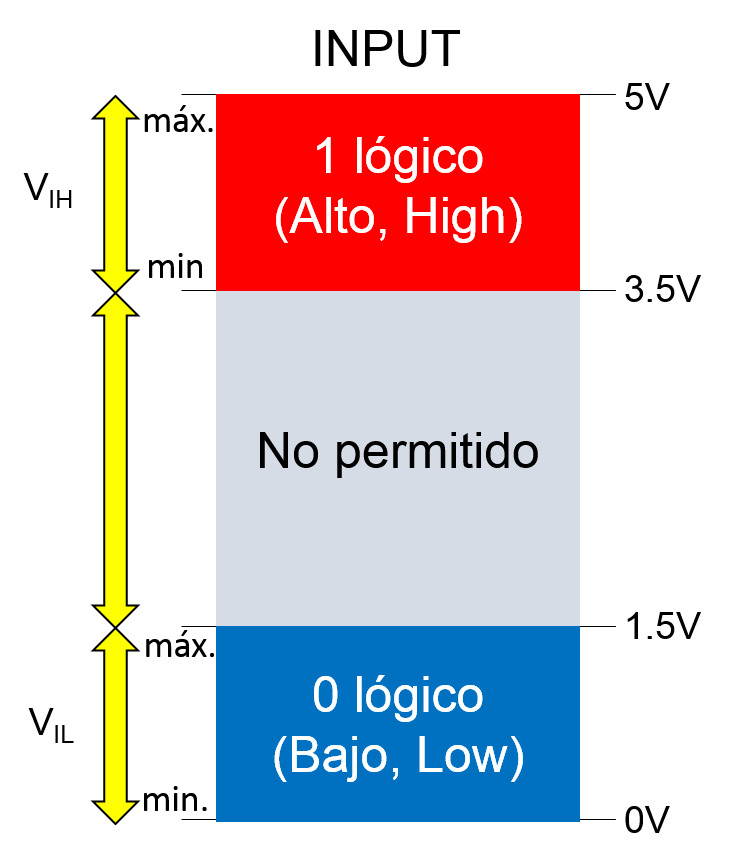
\includegraphics[scale=0.5]{SD/SD23.png}}
\subfloat[Salida]{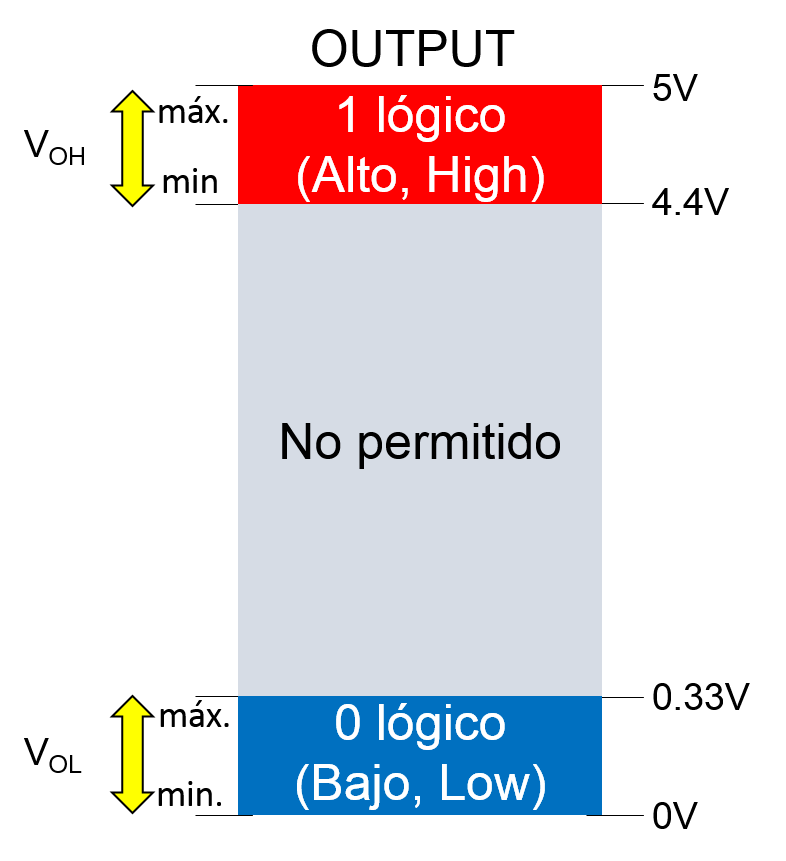
\includegraphics[scale=0.5]{SD/SD24.png}}
\caption{Nivel lógico CMOS a +5V.}
\end{figure}
%\pagebreak
\subsection{Nivel lógico CMOS +3V}
\begin{figure}[H]
\centering
\subfloat[Entrada]{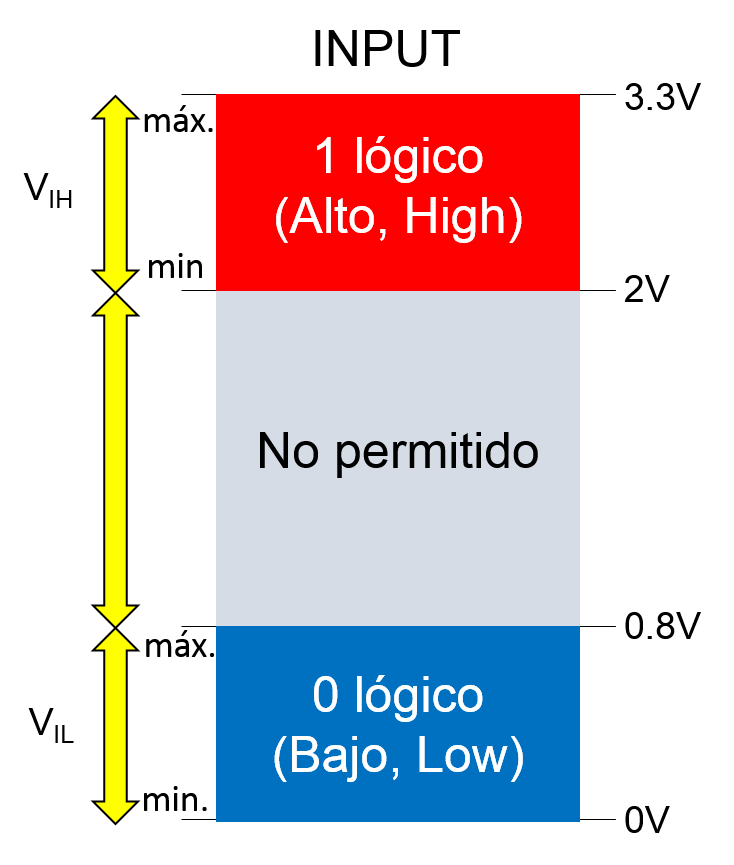
\includegraphics[scale=0.5]{SD/SD25.png}}
\subfloat[Salida]{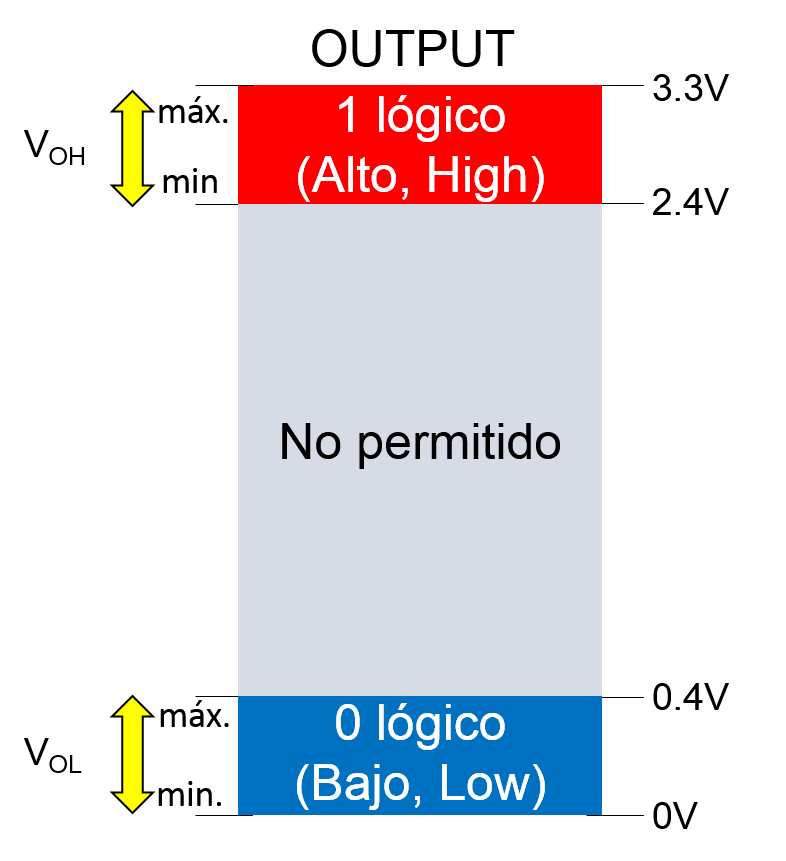
\includegraphics[scale=0.5]{SD/SD26.png}}
\caption{Nivel lógico CMOS a +3.3V.}
\end{figure}
\pagebreak
\subsection{Nivel lógico TTL}
\begin{figure}[H]
\centering
\subfloat[Entrada]{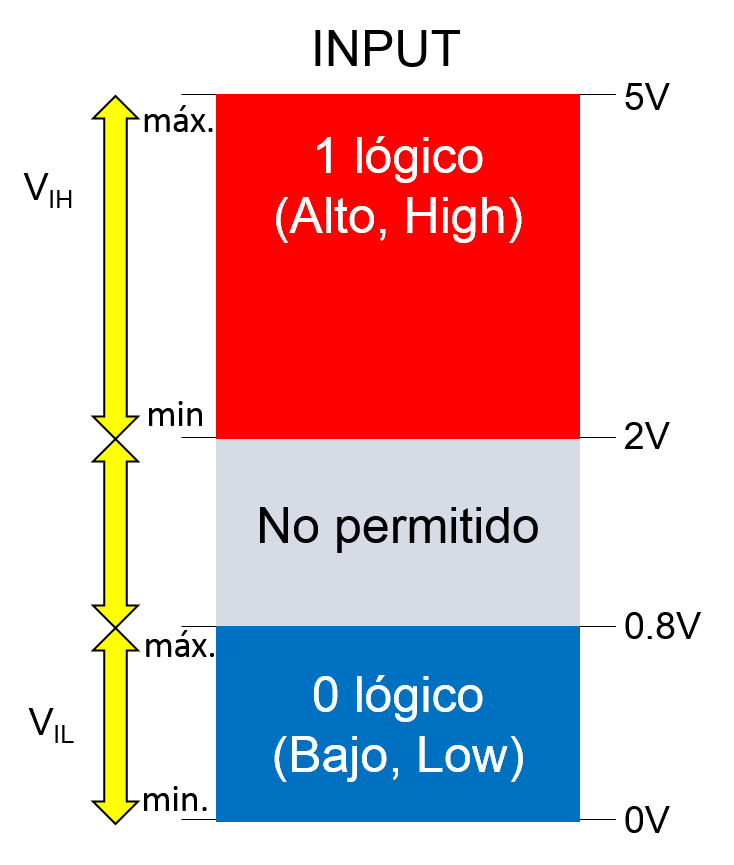
\includegraphics[scale=0.5]{SD/SD27.png}}
\subfloat[Salida]{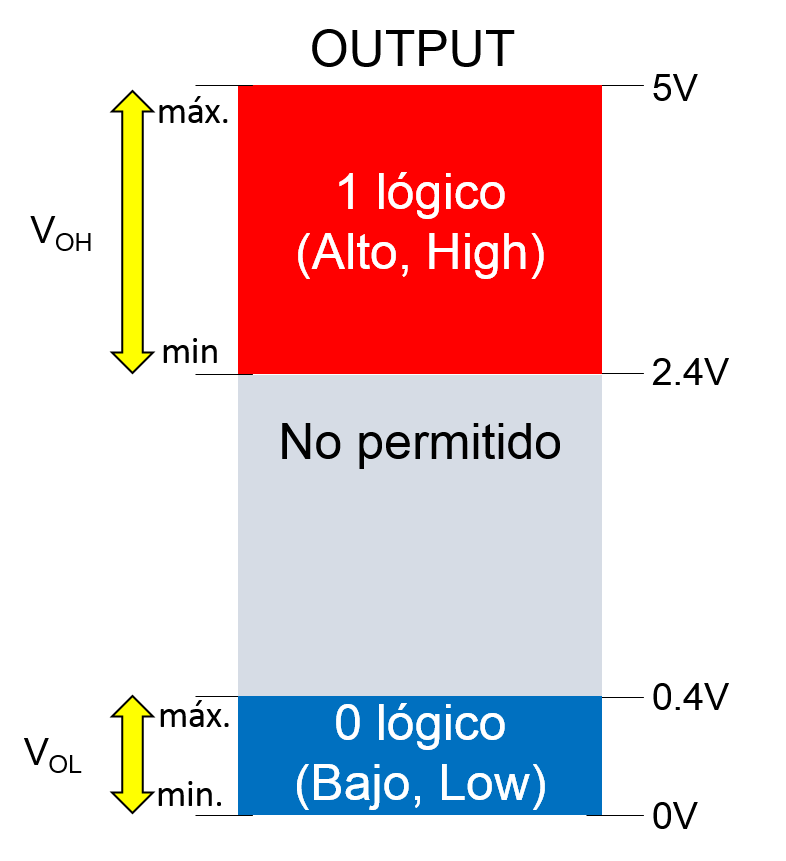
\includegraphics[scale=0.5]{SD/SD28.png}}
\caption{Nivel lógico TTL a +3.3V.}
\end{figure}
\subsection{Inmunidad y Margen de ruido}
Capacidad de tolerar ciertas fluctuaciones de tensión no deseadas en sus entradas sin que cambie. La medida de inmunidad de ruido es el margen de ruido. Para determinado circuito se especifican dos valores:
\begin{itemize}
\item[$V_{NH}$] Margen de ruido alto.
\item[$V_{NL}$] Margen de ruido bajo.
\end{itemize}
\begin{subequations}
\begin{align}
V_{NH}&=V_{OH(min)}-V_{IH(min)}
\label{eq:vnh} \\
V_{NL}&=V_{IL(máx)}-V_{OL(máx)}
\label{eq:vnl}
\end{align}
\label{eq:inmunidadruido}
\end{subequations}
\subsection{Disipación de potencia}
Cuando el estado de salida de la puerta es n nivel alto, circula la corriente $I_{CCH}$ y cuando es nivel bajo circula una corriente $I_{CCL}$.
\begin{equation}\label{eq:disipaciondepotencia}
I_{CC}=\frac{I_{CCH}+I_{ICCL}}{2}
\end{equation}
\begin{example}
Por una determinada puerta circulan 2$\mu$ A cuando su salida esta a nivel Alto y 3.6$\mu$ A cuando esta a nivel bajo. ¿Cual es la disipación de potencia media si:
\begin{itemize}
\item La puerta esta en un estado de salida estático alto?
\item La puerta esta en un estado de salida estático bajo?
\item $V_{cc}$ es 5V y la puerta funciona con un ciclo de trabajo de 25\% en alto?
\end{itemize}
\textbf{Solución:}\\
\begin{enumerate}
\item \textbf{Puerta estática en estado alto:}
\begin{align*}
&P=I\times V\\
&P=2\mu A \times 5V\\
&P=10\mu W
\end{align*}
\item \textbf{Puerta estática en estado bajo:}
\begin{align*}
&P=I\times V\\
&P=3.6\mu A \times 10V\\
&P=18\mu W
\end{align*}
La potencia media es:
\begin{displaymath}
P_m=\frac{10\mu W + 18\mu W}{2}=14\mu W
\end{displaymath}
\item \textbf{$V_{CC}$ es 5 V y nivel alto a 25\%}: 25\%  duty cycle es otra forma de expresar, esta forma es usada en PWM.\\
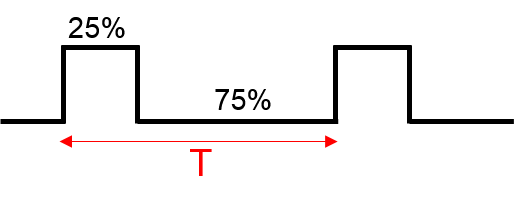
\includegraphics[scale=0.5]{SD/SD29.png}
\begin{align*}
&P=25\%(10\mu W)+75\%(14\mu W)\\
&P=2.5\mu W + 13.5 \mu W\\
&P=16W
\end{align*}\\
\end{enumerate}
\end{example}
La disposición en un circuito TTL es escencialmente constante denstro de su rango de frecuencias de operación. Para los CMOS depende de la frecuencia.
\begin{figure}[H]
\centering
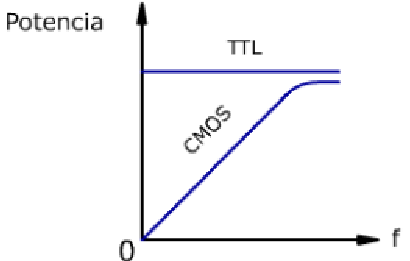
\includegraphics[scale=1]{SD/SD30.png}
\caption{Curva disipación de potencia.}
\end{figure}
\subsection{Carga y Fan-out}
Cuando la salida de una compuerta es la entrada de otra, esto se convierte en carga. Fan-out es el limite de cuantas puertas se puede colocar.
\chapter{Circuitos Lógicos}
Existen dos tipos de circuitos lógicos:
\begin{enumerate}
\item[Combinacional] Donde la salida solo depende de la entrada actual.
\item[Secuencial] Donde la salida depende de la entrada actual y la secuencia anterior.
\end{enumerate}
\section{Sumador}\index{Sumador}
\subsection{Semi-sumador}
\begin{figure}[H]
\centering
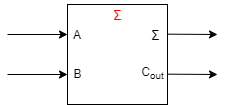
\includegraphics[scale=0.5]{SD/SD31.png}
\caption{Semi-sumador}
\label{fig:semisumador}
\end{figure}
\begin{itemize}
\item[A y B] Bits de entrada.
\item[$\Sigma$] Suma.
\item[$C_{out}$] Acarreo de salida.
\end{itemize}
Su tabla de verdad es la siguiente:\\
\begin{table}[H]
\begin{center}
\begin{tabular}{|c|c|c|c|}
\hline
\rowcolor{red}
A & B & $C_{out}$ & $\Sigma$ \\ \hline
0 & 0 & 0 & 0 \\ \hline
0 & 1 & 0 & 1 \\ \hline
1 & 0 & 0 & 1 \\ \hline
1 & 1 & 1 & 0 \\ \hline
\end{tabular}
\caption{Tabla de verdad: semi-sumador}
\label{tab:semisumador}
\end{center}
\end{table}
Las dos entradas dos A y B, las suma en binario de ambas entradas es la salida $\Sigma$ y el acarreo\footnote{Por ejemplo, 5+3=8, no existe acarreo. Pero si sumamos 8+9, sería 4 con acarreo de 1, en total 14. El acarreo depende del sistema de numeración. en base 10, el valor máximo es 9 ya que 10 será 0 con acarreo de 1; en base 2 ocurre lo mismo lo máximo será 10(2 en base 10).}(lo que comúnmente llamamos: "lo que llevamos") es la salida $C_{out}$. Ese circuito solo depende de las entradas actuales por si mismo. Para implementar este circuito, se tiene que implementar el siguiente circuito lógico:
\begin{figure}[H]
\centering
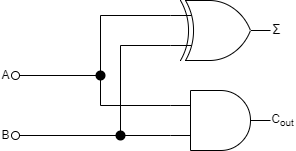
\includegraphics[scale=0.5]{SD/SD32.png}
\caption{Circuito lógico semi sumador}
\label{fig:CLsemisumador}
\end{figure}
\subsection{Sumador completo}
\begin{figure}[H]
\centering
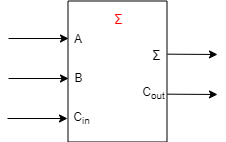
\includegraphics[scale=0.5]{SD/SD33.png}
\caption{Sumador completo}
\label{fig:sumadorcompleto}
Donde:
\begin{itemize}
\item[A y B] Bits de entrada.
\item[$C_{in}$] Acarreo de entrada.
\item[$\Sigma$] Suma.
\item[$C_{out}$] Acarreo de salida.
\end{itemize}
\end{figure}
La tabla de verdad del sumador completo es:
\begin{table}[]
\begin{center}
\begin{tabular}{|c|c|c|c|c|}
\hline
\rowcolor{color1}
A & B & $C_{in}$ & $C_{out}$ & $\Sigma$ \\ \hline
0 & 0 & 0        & 0         & 0        \\ \hline
0 & 0 & 1        & 0         & 1        \\ \hline
0 & 1 & 0        & 0         & 1        \\ \hline
0 & 1 & 1        & 1         & 0        \\ \hline
1 & 0 & 0        & 0         & 1        \\ \hline
1 & 0 & 1        & 1         & 0        \\ \hline
1 & 1 & 0        & 1         & 0        \\ \hline
1 & 1 & 1        & 1         & 1        \\ \hline
\end{tabular}
\end{center}
\caption{Tabla de verdad: Sumador completo.}
\label{tab:sumadorcompleto}
\end{table}
Simplificando por mapas de Karnaugh, se obtiene el siguiente circuito lógico:
\begin{figure}[H]
\centering
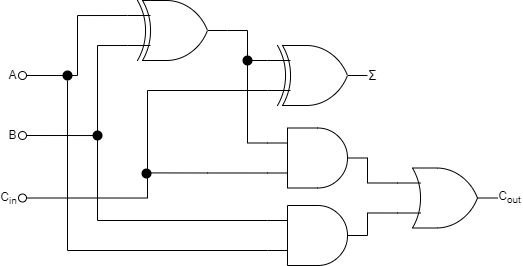
\includegraphics[scale=0.5]{SD/SD34.png}
\caption{Circuito lógico sumador completo}
\label{fig:CLsumadorcompleto}
\end{figure}
\subsection{Sumador paralelo}
Si implementamos los sumadores completo en cascada se obtiene el sumador en paralelo, que tiene la capacidad de sumar números con más dígitos.
\begin{figure}[H]
\centering
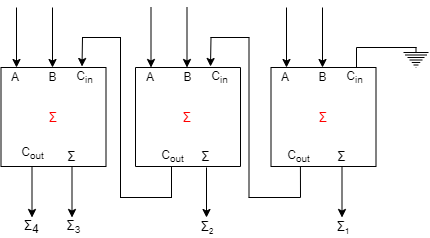
\includegraphics[scale=0.5]{SD/SD35.png}
\caption{Sumador paralelo}
\label{fig:sumadorparalelo}
\end{figure}
\subsection{Sumador 74LS283}
Este es un circuito que sirve como sumador de dos números de 4 bits, se puede encadenar más circuitos en forma de cascada para expandir el tamaño. Para poder usar este sumador se debe seguir los siguientes pasos:
\begin{enumerate}
\item \textbf{Identificar los números}: En nuestro ejemplo, usaremos B=22 y A=9.
\item \textbf{Pasar números a binario}: Si se desea la suma, solo se pasa a binario. Si se desea una resta, por ejemplo 22+(-9), en necesario pasar a binario ambos números y el número negativo se tiene que negar usando complemento a 1.
\item \textbf{Colocar los números en las entradas}: Para la suma: B=22=0001 0110 y A=9=0000 1001 en caso de la suma, en caso de resta: B=22=0001 0110 y A=-9=1111 0110. En este caso el tamaño de cada número es 1 byte, y están agrupados en grupos de 4 bits. Colocamos en las entradas en grupos de 4 bits empezando con el MSB.\\
Para la suma:
\begin{itemize}
\item \textbf{B(1-4)}: Colocamos 0001.
\item \textbf{A(1-4)}: Colocamos 0000.
\item \textbf{B(5-8)}: Colocamos 0110.
\item \textbf{A(5-8)}: Colocamos 1001.
\item \textbf{Interruptor Suma/Resta}: Este es un interruptor que conmuta entre una suma y resta, como sumaremos 22+9 lo dejamos en 0.
\end{itemize}
Para la resta:
\begin{itemize}
\item \textbf{B(1-4)}: Colocamos 0001.
\item \textbf{A(1-4)}: Colocamos 1111.
\item \textbf{B(5-8)}: Colocamos 0110.
\item \textbf{A(5-8)}: Colocamos 0110.
\item \textbf{Interruptor Suma/Resta}: Al tratarse de una resta 22+(-9) lo dejamos en 1.
\end{itemize}
\end{enumerate}
\begin{figure}[H]
\centering
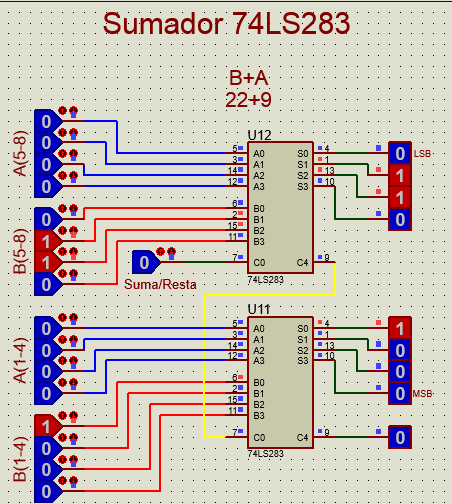
\includegraphics[scale=0.5]{SD/SD36.png}
\caption{Sumador 74LS283 en proteus.}
\end{figure}
\subsection{Sumador Acarreo Anticipado}
La propagación de acarreo tiene lugar cuando el acarreo de entrada se trasnmite como acarreo de salida. El acarre de entrada puede ser propagado por el sumador completo cuando uno o ambos bits de entrada son igual o 1. El acarreo propagado($C_p$) se expresa como la función OR de los bits de entrada.
\begin{displaymath}
C_p = A + B
\end{displaymath}
La generación tiene lugar cuando el sumador completo genera internamente un acarreo de salida. Solo cuando ambos bits de entrada son se genera internamente un acarreo de salida. Solo cuando ambos bits de entrada son 1 se genera un acarreo, el acarreo acelerado $C_g$ se expresa como la función AND de los bits de entrada A y B.
\begin{displaymath}
C_g = A\cdot B
\end{displaymath}
\begin{figure}[H]
\centering
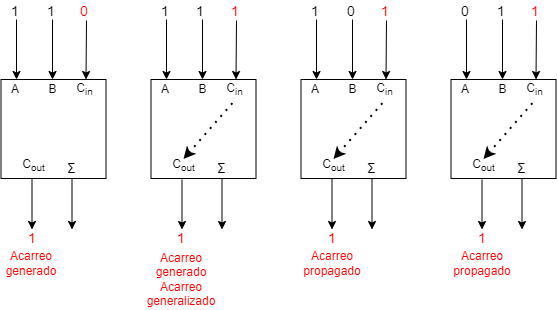
\includegraphics[scale=0.5]{SD/SD37.png}
\caption{Sumador anticipado.}
\label{fig:sumadoranticipado}
\end{figure}
\section{Codificador y Decodificador}\index{Codificador y Decodificador}
Es el proceso de asignar a cada entrada una combinación única de bits.
\subsection{Encoder}
Son circuitos combinacionales con $2^n$ entradas máximas y \textit{n} salidas, en donde las filas de las entradas van a tener \textbf{solo un dato que cambia} y en la salida aparece un código asignado a esas entradas.
\subsubsection{Procedimiento}
\begin{enumerate}
\item Determine cual es el único valor que cambia en la entrada.
\item Las salidas se leen por columnas tomando cada dato como un término completo.
\end{enumerate}
\begin{itemize}
\item \textbf{Caso 1: En cada fila hay un dato que cambia.} En un teclado se utilizan teclas del 0 al 3 y se requiere que en las salidas entregue los números codificados en binario en las entradas.
\begin{table}[h]
\begin{center}
\begin{tabular}{|cccc|cc|}
\hline
\rowcolor{color1}
\multicolumn{4}{|c|}{IN}                                                                      & \multicolumn{2}{c|}{OUT}           \\ \hline
\rowcolor{color1!80}
\multicolumn{1}{|c|}{$T_0$} & \multicolumn{1}{c|}{$T_1$} & \multicolumn{1}{c|}{$T_2$} & $T_3$ & \multicolumn{1}{c|}{$B_0$} & $B_1$ \\ \hline
\multicolumn{1}{|c|}{\textcolor{red}{1}}     & \multicolumn{1}{c|}{0}     & \multicolumn{1}{c|}{0}     & 0     & \multicolumn{1}{c|}{0}     & 0     \\ \hline
\multicolumn{1}{|c|}{0}     & \multicolumn{1}{c|}{\textcolor{red}{1}}     & \multicolumn{1}{c|}{0}     & 0     & \multicolumn{1}{c|}{0}     & 1     \\ \hline
\multicolumn{1}{|c|}{0}     & \multicolumn{1}{c|}{0}     & \multicolumn{1}{c|}{\textcolor{red}{1}}     & 0     & \multicolumn{1}{c|}{1}     & 0     \\ \hline
\multicolumn{1}{|c|}{0}     & \multicolumn{1}{c|}{0}     & \multicolumn{1}{c|}{0}     & \textcolor{red}{1}     & \multicolumn{1}{c|}{1}     & 1     \\ \hline
\end{tabular}
\caption{Tabla de verdad codificador 3 botones.}
\end{center}
\end{table}
La realización de esta tabla cumple con: $2^2=4$ entradas y 2 salidas. El dato que cambia es la entrada 1, si lo escribimos como POS y SOP:
\begin{align*}
B_1&=T_1+T_3\\
B_2&=T_2+T_3\\
B_1&=\overline{T_0}\cdot \overline{T_2}\\
B_2&=\overline{T_0}\cdot \overline{T_1}
\end{align*}
\item \textbf{Caso 2: Hay una fila donde ningún dato cambia.}
\begin{table}[h]
\begin{center}
\begin{tabular}{|ccc|cc|}
\hline
\rowcolor{color1}
\multicolumn{3}{|c|}{IN}                                         & \multicolumn{2}{c|}{OUT}   \\ \hline
\rowcolor{color1!80}
\multicolumn{1}{|c|}{$D_0$} & \multicolumn{1}{c|}{$D_1$} & $D_2$ & \multicolumn{1}{c|}{B} & A \\ \hline
\multicolumn{1}{|c|}{0}     & \multicolumn{1}{c|}{1}     & 1     & \multicolumn{1}{c|}{0} & 0 \\ \hline
\multicolumn{1}{|c|}{1}     & \multicolumn{1}{c|}{0}     & 1     & \multicolumn{1}{c|}{0} & 1 \\ \hline
\multicolumn{1}{|c|}{1}     & \multicolumn{1}{c|}{1}     & 0     & \multicolumn{1}{c|}{1} & 0 \\ \hline
\multicolumn{1}{|c|}{1}     & \multicolumn{1}{c|}{1}     & 1     & \multicolumn{1}{c|}{1} & 1 \\ \hline
\end{tabular}
\caption{Codificador: una fila no cambia.}
\end{center}
\end{table}
\begin{align*}
A&=\overline{D_1}+(D_0\cdot D_1\cdot D_2)\\
B&=\overline{D_2}+(D_0\cdot D_1\cdot D_2)\\
A&=D_0\cdot D_2\\
B&=D_0\cdot D_1
\end{align*}
\item \textbf{Hay una fila donde todos los datos cambian.}
\begin{table}[]
\begin{center}
\begin{tabular}{|ccc|cc|}
\hline
\rowcolor{color1}
\multicolumn{3}{|c|}{IN}                                         & \multicolumn{2}{c|}{OUT}   \\ \hline
\rowcolor{color1!80}
\multicolumn{1}{|c|}{$D_0$} & \multicolumn{1}{c|}{$D_1$} & $D_2$ & \multicolumn{1}{c|}{B} & A \\ \hline
\multicolumn{1}{|c|}{0}     & \multicolumn{1}{c|}{1}     & 1     & \multicolumn{1}{c|}{0} & 0 \\ \hline
\multicolumn{1}{|c|}{1}     & \multicolumn{1}{c|}{0}     & 1     & \multicolumn{1}{c|}{1} & 1 \\ \hline
\multicolumn{1}{|c|}{1}     & \multicolumn{1}{c|}{1}     & 0     & \multicolumn{1}{c|}{1} & 0 \\ \hline
\multicolumn{1}{|c|}{0}     & \multicolumn{1}{c|}{0}     & 0     & \multicolumn{1}{c|}{0} & 1 \\ \hline
\end{tabular}
\end{center}
\end{table}
\begin{align*}
A&=\overline{D_1}+(\overline{D_0}\cdot \overline{D_1}\cdot \overline{D_2})\\
B&=\overline{D_1}+\overline{D_2}\\
A&=D_0\cdot D_2\\
B&=D_0\cdot (D_0+D_1+D_2)
\end{align*}
\end{itemize}
Tipos:
\begin{itemize}
\item \textbf{Sin prioridad}: Solamente una entrada puede ser activada en cada instante.
% Please add the following required packages to your document preamble:
% \usepackage[table,xcdraw]{xcolor}
% If you use beamer only pass "xcolor=table" option, i.e. \documentclass[xcolor=table]{beamer}
\begin{table}[h]
\begin{center}
\begin{tabular}{|cccccccc|ccc|}
\hline
\multicolumn{8}{|c|}{IN}                                                                                                                                                                                                                                                                                                                                                  & \multicolumn{3}{c|}{OUT}                                        \\ \hline
\multicolumn{1}{|c|}{$A_0$}                    & \multicolumn{1}{c|}{$A_1$}                    & \multicolumn{1}{c|}{$A_2$}                    & \multicolumn{1}{c|}{$A_3$}                    & \multicolumn{1}{c|}{$A_4$}                    & \multicolumn{1}{c|}{$A_5$}                    & \multicolumn{1}{c|}{$A_6$}                    & $A_7$                    & \multicolumn{1}{c|}{$Y_2$} & \multicolumn{1}{c|}{$Y_1$} & $Y_0$ \\ \hline
\multicolumn{1}{|c|}{{\color[HTML]{FE0000} 0}} & \multicolumn{1}{c|}{1}                        & \multicolumn{1}{c|}{1}                        & \multicolumn{1}{c|}{1}                        & \multicolumn{1}{c|}{1}                        & \multicolumn{1}{c|}{1}                        & \multicolumn{1}{c|}{1}                        & 1                        & \multicolumn{1}{c|}{0}     & \multicolumn{1}{c|}{0}     & 0     \\ \hline
\multicolumn{1}{|c|}{1}                        & \multicolumn{1}{c|}{{\color[HTML]{FE0000} 0}} & \multicolumn{1}{c|}{1}                        & \multicolumn{1}{c|}{1}                        & \multicolumn{1}{c|}{1}                        & \multicolumn{1}{c|}{1}                        & \multicolumn{1}{c|}{1}                        & 1                        & \multicolumn{1}{c|}{0}     & \multicolumn{1}{c|}{0}     & 1     \\ \hline
\multicolumn{1}{|c|}{1}                        & \multicolumn{1}{c|}{1}                        & \multicolumn{1}{c|}{{\color[HTML]{FE0000} 0}} & \multicolumn{1}{c|}{1}                        & \multicolumn{1}{c|}{1}                        & \multicolumn{1}{c|}{1}                        & \multicolumn{1}{c|}{1}                        & 1                        & \multicolumn{1}{c|}{0}     & \multicolumn{1}{c|}{1}     & 0     \\ \hline
\multicolumn{1}{|c|}{1}                        & \multicolumn{1}{c|}{1}                        & \multicolumn{1}{c|}{1}                        & \multicolumn{1}{c|}{{\color[HTML]{FE0000} 0}} & \multicolumn{1}{c|}{1}                        & \multicolumn{1}{c|}{1}                        & \multicolumn{1}{c|}{1}                        & 1                        & \multicolumn{1}{c|}{0}     & \multicolumn{1}{c|}{1}     & 1     \\ \hline
\multicolumn{1}{|c|}{1}                        & \multicolumn{1}{c|}{1}                        & \multicolumn{1}{c|}{1}                        & \multicolumn{1}{c|}{1}                        & \multicolumn{1}{c|}{{\color[HTML]{FE0000} 0}} & \multicolumn{1}{c|}{1}                        & \multicolumn{1}{c|}{1}                        & 1                        & \multicolumn{1}{c|}{1}     & \multicolumn{1}{c|}{0}     & 0     \\ \hline
\multicolumn{1}{|c|}{1}                        & \multicolumn{1}{c|}{1}                        & \multicolumn{1}{c|}{1}                        & \multicolumn{1}{c|}{1}                        & \multicolumn{1}{c|}{1}                        & \multicolumn{1}{c|}{{\color[HTML]{FE0000} 0}} & \multicolumn{1}{c|}{1}                        & 1                        & \multicolumn{1}{c|}{1}     & \multicolumn{1}{c|}{0}     & 1     \\ \hline
\multicolumn{1}{|c|}{1}                        & \multicolumn{1}{c|}{1}                        & \multicolumn{1}{c|}{1}                        & \multicolumn{1}{c|}{1}                        & \multicolumn{1}{c|}{1}                        & \multicolumn{1}{c|}{1}                        & \multicolumn{1}{c|}{{\color[HTML]{FE0000} 0}} & 1                        & \multicolumn{1}{c|}{1}     & \multicolumn{1}{c|}{1}     & 0     \\ \hline
\multicolumn{1}{|c|}{1}                        & \multicolumn{1}{c|}{1}                        & \multicolumn{1}{c|}{1}                        & \multicolumn{1}{c|}{1}                        & \multicolumn{1}{c|}{1}                        & \multicolumn{1}{c|}{1}                        & \multicolumn{1}{c|}{1}                        & {\color[HTML]{FE0000} 0} & \multicolumn{1}{c|}{1}     & \multicolumn{1}{c|}{1}     & 1     \\ \hline
\end{tabular}
\end{center}
\end{table}
\begin{align*}
Y_0&=\overline{A_1}+\overline{A_3}+\overline{A_5}+\overline{A_7} \therefore Y_0=\overline{A_1\times A_3\times A_5\times A_7}\\
Y_1&=\overline{A_2}+\overline{A_3}+\overline{A_6}+\overline{A_7} \therefore Y_1=\overline{A_2\times A_3\times A_6\times A_7}\\
Y_2&=\overline{A_4}+\overline{A_5}+\overline{A_6}+\overline{A_7} \therefore Y_0=\overline{A_4\times A_5\times A_6\times A_7}\\
\end{align*}
Las entradas se activan con 0 lógico.
\item \textbf{Con prioridad}: Codifica la entrada activa de mayor valor decimal son tener en cuenta los demás.
Un ejemplo con prioridad es el IC74147, donde todas las entradas se activan con 0 lógico y las todas las salidas están negadas, es decir, se activan con 0 lógico.
\end{itemize}
\subsection{Decoder}
Al contrario del encoder, el decoder es lo contrario: de \textit{n} entradas se puede manipular $2^n$ entradas. El número en binario se escribe empezando por el A1 (que es más significativo). Los decodificadores tienen su propia tabla de la verdad que representa los estado posibles de entrada y los respectivos valores de las salidas para cada uno de esos estados.\\
De esta tabla de la verdad podemos sacar el circuito lógico combinacional con puertas lógicas, circuito lógico para construir nuestro decodificador.
\begin{example}
Diseñe 2 circuitos que al activarse cada uno de los pulsadores en la salida se visualicen los siguientes números en binario:
\begin{enumerate}
\item Pulsador 1: 14
\item Pulsador 2: 50
\item Pulsador 3: 23
\item Pulsador 4: 72
\end{enumerate}
\textbf{Solución:}\\
Primero, vamos a separar decenas y unidades de cada número y diseñar una tabla de verdad para cada uno. Solo poseemos 4 pulsadores, por lo tanto, vamos a necesitar 3 salidas puesto que los números de las decenas(1, 5, 2, 7) expresadas en binario necesitan 3 dígitos; entonces para n=3 salidas nos podemos permitir $2^3=8$ entradas, pero solo haremos uso de 4 entradas. Nuestro circuito constará de dos sub-circuitos: uno se encargará de mostrar los dígitos de las decenas y el otro mostrará los dígitos de las unidades. Desarrollamos la tabla de verdad para las decenas.\\
\begin{center}
\begin{tabular}{|cccc|ccc|c|}
\hline
\rowcolor{ocre!70}
\multicolumn{4}{|c|}{INPUT}                                                                                                                                               & \multicolumn{3}{c|}{OUTPUT}                                     &       \\ \hline
\rowcolor{ocre!50}
\multicolumn{1}{|c|}{$P_1$}                    & \multicolumn{1}{c|}{$P_2$}                    & \multicolumn{1}{c|}{$P_3$}                    & $P_4$                    & \multicolumn{1}{c|}{$D_2$} & \multicolumn{1}{c|}{$D_1$} & $D_0$ & $N_0$ \\ \hline
\multicolumn{1}{|c|}{{\color[HTML]{FE0000} 1}} & \multicolumn{1}{c|}{0}                        & \multicolumn{1}{c|}{0}                        & 0                        & \multicolumn{1}{c|}{0}     & \multicolumn{1}{c|}{0}     & 1     & 1     \\ \hline
\multicolumn{1}{|c|}{0}                        & \multicolumn{1}{c|}{{\color[HTML]{FE0000} 1}} & \multicolumn{1}{c|}{0}                        & 0                        & \multicolumn{1}{c|}{1}     & \multicolumn{1}{c|}{0}     & 1     & 5     \\ \hline
\multicolumn{1}{|c|}{0}                        & \multicolumn{1}{c|}{0}                        & \multicolumn{1}{c|}{{\color[HTML]{FE0000} 1}} & 0                        & \multicolumn{1}{c|}{0}     & \multicolumn{1}{c|}{1}     & 0     & 2     \\ \hline
\multicolumn{1}{|c|}{0}                        & \multicolumn{1}{c|}{0}                        & \multicolumn{1}{c|}{0}                        & {\color[HTML]{FE0000} 1} & \multicolumn{1}{c|}{1}     & \multicolumn{1}{c|}{1}     & 1     & 7     \\ \hline
\end{tabular}
\end{center}
Una vez que hayamos desarrollado nuestra tabla de verdad las simplificamos usando POS o SOP, es preciso decir que ambos son posibles pero como hablamos de \textbf{SIMPLIFICAR} usaremos el que menos términos genere, en otras palabras: la salida $D_0$ posee 3 salidas en 1(SOP), esa misma salida posee 1 salida en 0(POS), entonces nos combiene POS pues solo será un término comprado a los 3 que nos generaría la otra forma. Aplicando POS a la tabla de las decenas:
\begin{align*}
D_0&=\overline{P_3}\\
D_1&=\overline{P_1}\times\overline{P_2}\\
D_2&=\overline{P_1}\times\overline{P_3}
\end{align*}
Lo mismo haremos con las unidades, sin embargo en esta tabla notamos que nos conviene expresarlo como SOP pues en cada salida hay menos salidas 1 que salidas 0, por lo tanto, simplificando mediante SOP la tabla de las unidades:
\begin{center}
\begin{tabular}{|cccc|ccc|c|}
\hline
\rowcolor{ocre!70}
\multicolumn{4}{|c|}{INPUT}                                                                                                                                               & \multicolumn{3}{c|}{OUTPUT}                                     &       \\ \hline
\rowcolor{ocre!50}
\multicolumn{1}{|c|}{$P_1$}                    & \multicolumn{1}{c|}{$P_2$}                    & \multicolumn{1}{c|}{$P_3$}                    & $P_4$                    & \multicolumn{1}{c|}{$D_2$} & \multicolumn{1}{c|}{$D_1$} & $D_0$ & $N_0$ \\ \hline
\multicolumn{1}{|c|}{{\color[HTML]{FE0000} 1}} & \multicolumn{1}{c|}{0}                        & \multicolumn{1}{c|}{0}                        & 0                        & \multicolumn{1}{c|}{1}     & \multicolumn{1}{c|}{0}     & 0     & 4     \\ \hline
\multicolumn{1}{|c|}{0}                        & \multicolumn{1}{c|}{{\color[HTML]{FE0000} 1}} & \multicolumn{1}{c|}{0}                        & 0                        & \multicolumn{1}{c|}{0}     & \multicolumn{1}{c|}{0}     & 0     & 0     \\ \hline
\multicolumn{1}{|c|}{0}                        & \multicolumn{1}{c|}{0}                        & \multicolumn{1}{c|}{{\color[HTML]{FE0000} 1}} & 0                        & \multicolumn{1}{c|}{0}     & \multicolumn{1}{c|}{1}     & 1     & 3     \\ \hline
\multicolumn{1}{|c|}{0}                        & \multicolumn{1}{c|}{0}                        & \multicolumn{1}{c|}{0}                        & {\color[HTML]{FE0000} 1} & \multicolumn{1}{c|}{0}     & \multicolumn{1}{c|}{1}     & 0     & 2     \\ \hline
\end{tabular}
\end{center}
\begin{align*}
U_0&=P_3\\
U_1&=P_3 + P_4\\
U_2&=P_1
\end{align*}Ya tenemos las expresiones, antes de realizar el circuito esta de más aclarar que el bit más significativo es en el caso de las decenas $D_2$ y en el caso de las unidades es $U_2$. Tenemos las expresiones booleanas de cada tabla así que solo queda realizar su circuito:\\
\begin{center}
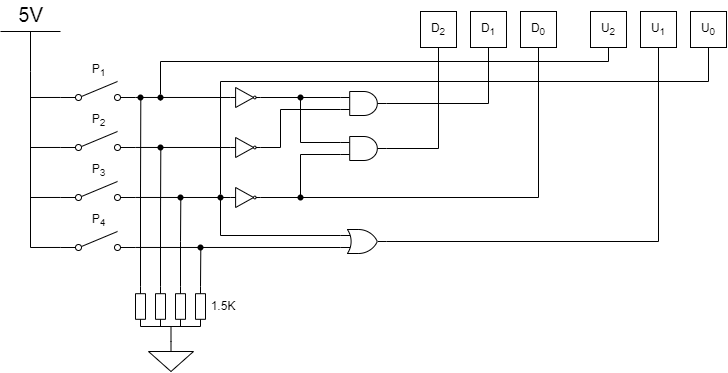
\includegraphics[scale=0.4]{SD/SD38.png}
\end{center}
\end{example}
\section{Multiplexor y Demultiplexor}\index{Multiplexor y Demultiplexor}
\subsection{Multiplexor}
Circuito combinacional al que entran varios canales y solo sale uno de ellos.
\begin{center}
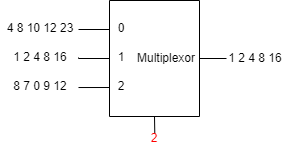
\includegraphics[scale=0.8]{SD/SD39.png}
\end{center}
\subsubsection{Multiplexor Simple}
Existen dos posibles simbologías para los multiplexores:
\begin{center}
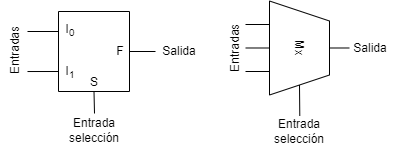
\includegraphics[scale=0.8]{SD/SD40.png}
\end{center}
\begin{multicols}{2}
\begin{center}
\begin{tabular}{|c|c|c|c|}
\hline
\rowcolor{ocre!70}
S & $I_1$ & $I_1$ & F \\ \hline
0 & 0     & 0     & 0 \\ \hline
0 & 0     & 1     & 1 \\ \hline
0 & 1     & 0     & 0 \\ \hline
0 & 1     & 1     & 1 \\ \hline
1 & 0     & 0     & 0 \\ \hline
1 & 0     & 1     & 0 \\ \hline
1 & 1     & 0     & 1 \\ \hline
1 & 1     & 1     & 1 \\ \hline
\end{tabular}
\end{center}
\columnbreak
\begin{center}
\begin{karnaugh-map}[4][2][1][$I_1I_0$][$S$]
\minterms{1,3,6,7}
\maxterms{0,2,5,4}
\end{karnaugh-map}
\begin{displaymath}
F=\overline{S}\cdot I_0 + S\cdot I_1
\end{displaymath}
\end{center}
\end{multicols}
\begin{remark}
Es usual que en las tablas de verdad, la entrada que se encuentra a la izquierda es el más significativo(MSB) mientras que el que se encuentra más a la derecha es el menos significativo(LSB).
\end{remark}
Si analizamos la tabla: vemos que la entrada de selección S, poseerá dos estados; si analizamos cuando S=0 vemos que la salida F estará activada siempre y cuando la entrada $I_0$ tenga la entrada activa, mientras que si $I_0$ posee una entrada 0, no importa el valor que posea la entrada $I_1$(alto o bajo) la salida F siempre será 0. Esto nos quiere decir que cuando S=0, la salida F solo le importará los estados de la entrada $I_0$ pero no de $I_1$. Cuando la entrada de selección S=1, notaremos le mismo comportamiento, la salida F solo tomará en cuenta los estados de la entrada $I_1$ puesto que la entrada $I_0$ no nos importa. En conclusión, el la entrada de control S es capaz de seleccionar entre dos entradas.
\subsubsection{Multiplexor 2 entradas selección}
\begin{multicols}{2}
\begin{center}
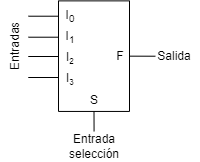
\includegraphics[scale=0.6]{SD/SD41.png}
\end{center}
\columnbreak
\begin{center}
\begin{tabular}{|c|c|c|}
\hline
\rowcolor{ocre!70}
$S_1$ & $S_0$ & F     \\ \hline
0     & 0     & $I_0$ \\ \hline
0     & 1     & $I_1$ \\ \hline
1     & 0     & $I_2$ \\ \hline
1     & 1     & $I_3$ \\ \hline
\end{tabular}
\begin{displaymath}
F=\overline{S_1}\cdot\overline{S_0}\cdot I_0+\overline{S_1}\cdot S_0\cdot I_1+S_1\cdot\overline{S_0}\cdot I_2+S_1\cdot S_0\cdot I_3
\end{displaymath}
\end{center}
\end{multicols}
\subsection{Demultiplexor}
Al igual que el multiplexor puede poseer varias entradas, varios canales a diferentes bits.
\begin{center}
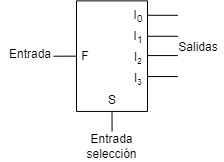
\includegraphics[scale=0.5]{SD/SD42.png}
\end{center}
La expresión booleana para el multiplexor más simple:
\begin{multicols}{2}
\begin{center}
\includegraphics[scale=0.6]{SD/SD43.png}
\end{center}
\columnbreak
\begin{center}
\begin{tabular}{|c|c|c|c|}
\hline
\rowcolor{ocre!70}
S & I & $O_1$ & $O_0$ \\ \hline
0 & 0 & 0     & 0     \\ \hline
0 & 1 & 0     & 1     \\ \hline
1 & 0 & 0     & 0     \\ \hline
1 & 1 & 1     & 0     \\ \hline
\end{tabular}
\begin{displaymath}
F=\overline{S_1}\cdot\overline{S_0}\cdot I_0+\overline{S_1}\cdot S_0\cdot I_1+S_1\cdot\overline{S_0}\cdot I_2+S_1\cdot S_0\cdot I_3
\end{displaymath}
\end{center}
\end{multicols}
\begin{multicols}{2}
\begin{center}
\includegraphics[scale=0.6]{SD/SD44.png}
\end{center}
\columnbreak
\begin{center}
\begin{tabular}{|c|c|c|c|c|c|}
\hline
\rowcolor{ocre!70}
$S_1$ & $S_1$ & $O_3$ & $O_2$ & $O_1$ & $O_0$ \\ \hline
0     & 0     & 0     & 0     & 0     & 1     \\ \hline
0     & 1     & 0     & 0     & 1     & 0     \\ \hline
1     & 0     & 0     & 1     & 0     & 0     \\ \hline
1     & 1     & 1     & 0     & 0     & 0     \\ \hline
\end{tabular}
\begin{align*}
&O_0=\overline{S_1}\cdot\overline{S_0}\cdot I
&O_1=\overline{S_1}\cdot\overline{S_0}\cdot I\\
&O_2=S_1\cdot\overline{S_0}\cdot I
&O_3=S_1\cdot S_0\cdot I
\end{align*}
\end{center}
\end{multicols}
\begin{example}
Usando el IC 74HCT4051, expresar la siguiente expresión de un demultiplexor:
\begin{displaymath}
F=C\overline{BA}+\overline{C}B\overline{A}+\overline{C}BA+CBA+\overline{CB}A
\end{displaymath}
\textbf{Solución:}\\
Para poder implementarlo con el IC, necesitamos que la expresión este en su forma canónica. Una vez que este en su forma canónica, dependiendo si esta como SOP o POS nos indicará los valores donde será 1 y 0 respectivamente. Como estamos frente a un SOP, los valores decimales de los sumandos(pasando a binario los bits, donde MSB es C y LSB es A) nos dan los números de las entradas en las cuales deben tener entradas altas y las restantes entrada baja.
\begin{center}
\includegraphics[scale=0.4]{SD/SD45.png}
\end{center}
Cada vez que en las entradas de selección se logre colocar cualquiera de los sumandos de la función F la salida será 1.
\end{example}
\section{Latch}\index{Latch}
El latch(cerrojo) es un tipo de dispositivo de almacenamiento temporal de dos estados(biestable).
\subsection{Latch S-R(Set-Reset)}
Dispositivo lógico biestable o multivibrador. Un Latch S-R con entrada activa a un nivel ALTO, se compone de dos puerta NOR o NAND acopladas.\\
\begin{figure}[H]
\centering
\includegraphics[scale=0.5]{SD/SD46.png}
\caption{Latch S-R con entrada activa a nivel alto.}
\label{fig:latchsrnor}
\end{figure}
\begin{figure}[H]
\centering
\includegraphics[scale=0.5]{SD/SD47.png}
\caption{Latch $\overline{S}$-$\overline{R}$ con entrada activa a nivel bajo.}
\label{fig:latchsrand}
\end{figure}
\subsubsection{Comportamiento}
En Q, cuando S este en nivel alto y R en estado bajo, la salida Q cambia a nivel alto(Estado inicial Q=0).\\
\begin{figure}[H]
\centering
\includegraphics[scale=0.5]{SD/SD48.png}
\caption{Set=1, Reset=0 y Q=1.}
\end{figure}
Una vez que nos encontramos en este estado, sea cual sea la entrada de S, la salida Q no cambiará:\\
\begin{figure}[H]
\centering
\includegraphics[scale=0.5]{SD/SD49.png}
\caption{Set=1/0, Reset=0 y Q=1.}
\end{figure}
Cambiará solo si R cambia a estado alto.\\
\begin{figure}[H]
\centering
\includegraphics[scale=0.5]{SD/SD50.png}
\caption{Set=0, Reset=1 y Q=0.}
\end{figure}
\subsubsection{Condiciones especiales}
Los latch poseen algunas restricciones que son importantes conocerlas para tener precaución al momento de implementar circuito.
\begin{figure}[H]
\centering
\includegraphics[scale=0.5]{SD/SD50.png}
\caption{Si S=0 y R=0, las salidas no cambian.}
\end{figure}
\begin{figure}[H]
\centering
\includegraphics[scale=0.5]{SD/SD51.png}
\caption{Si S=1 y R=1, las salidas presentan un estado no válido: indeterminado.}
\end{figure}
\subsection{Símbolo lógico}
La simbología del latch es el siguiente:
\begin{figure}
    \centering
    \subfloat[Latch $\overline{S}$-$\overline{R}$ con entrada activa BAJO.]{{\includegraphics[height=3cm]{SD/SD52.png} }}
    \qquad
    \subfloat[Latch S-R con entrada activa ALTA.]{{\includegraphics[height=3cm]{SD/SD53.png} }}
    \caption{Latch simbología}
\end{figure}
\begin{table}[h]
\begin{center}
\begin{tabular}{|cc|cc|c|}
\hline
\rowcolor{ocre!70}
\multicolumn{2}{|c|}{Input}                           & \multicolumn{2}{c|}{Output}              &                                         \\ \hline
\rowcolor{ocre!50}
\multicolumn{1}{|c|}{$\overline{S}$} & $\overline{R}$ & \multicolumn{1}{c|}{Q}  & $\overline{Q}$ & Comentarios                             \\ \hline
\multicolumn{1}{|c|}{1}              & 1              & \multicolumn{1}{c|}{NC} & NC             & No cambia, permanece en el mismo estado \\ \hline
\multicolumn{1}{|c|}{0}              & 1              & \multicolumn{1}{c|}{1}  & 0              & Latch estado SET                        \\ \hline
\multicolumn{1}{|c|}{1}              & 0              & \multicolumn{1}{c|}{0}  & 1              & Latch estado Reset                      \\ \hline
\multicolumn{1}{|c|}{1}              & 1              & \multicolumn{1}{c|}{1}  & 1              & Condición NO valida                     \\ \hline
\end{tabular}
\caption{Tabla de verdad: Latch}
\end{center}
\end{table}
El diagrama de tiempos de un Latch tiene el siguiente comportamiento ejemplificado:
\begin{figure}[H]
\centering
\includegraphics[scale=0.3]{SD/SD54.png}
\caption{Diagrama de tiempos Latch.}
\end{figure}
\subsection{Latch: Eliminador de rebote}
Se presenta un circuito con interruptor:\\
\begin{center}
\includegraphics[scale=0.5]{SD/SD55.png}
\end{center}
Vemos que la salida no es estable, esta lectura inestable puede ocasionar errores de lectura o falsos altos y bajos. Por eso se añade un latch como eliminador de rebote:\\
\begin{center}
\includegraphics[scale=0.5]{SD/SD56.png}
\end{center}
Usando un CI timer 555 se puede crear un sistema anti-rebote, en la figura \ref{fig:timer 555}.
\begin{figure}[H]
\centering
\includegraphics[width=0.6\linewidth]{SD/SD95.png}
\caption{Timer 555 usado como sistema anti-rebote.}
\label{fig:timer 555}
\end{figure}
\subsection{Latch con entrada de habilitación}
El latch no cambiará de estado hasta que la entrada EN este en nivel ALTO, mientras este en ALTO, las salidas serán controlados por las entradas S y R. Una situación invalida es cuando R y S están a nivel alto simultáneamente.
\begin{figure}[h]
    \centering
    \subfloat[Circuito Latch con entrada de habilitación.]{{\includegraphics[height=3cm]{SD/SD57.png} }}
    \qquad
    \subfloat[Simbología Latch con entrada de habilitación.]{{\includegraphics[height=3cm]{SD/SD58.png} }}
    \caption{Latch con entrada de habilitación.}
\end{figure}
Diagrama de tiempos de un Latch con entrada enable:
\begin{figure}[H]
\centering
\includegraphics[scale=0.3]{SD/SD59.png}
\caption{Diagrama de tiempos latch S-R con entrada de habilitación.}
\end{figure}
\subsection{Latch D con entrada de habilitación}
A diferencia de latch S-R con entrada de habilitación, el latch D solo tiene una entrada que recibe el nombre de entrada de datos(D) y ademas de la habilitación(EN).
\begin{figure}[h]
    \centering
    \subfloat[Circuito Latch D con entrada de habilitación.]{{\includegraphics[height=3cm]{SD/SD60.png} }}
    \qquad
    \subfloat[Simbología Latch D con entrada de habilitación.]{{\includegraphics[height=3cm]{SD/SD61.png} }}
    \caption{Latch D con entrada de habilitación.}
\end{figure}
\begin{figure}[H]
\centering
\includegraphics[scale=0.3]{SD/SD62.png}
\caption{Diagrama de tiempos latch D con entrada de habilitación.}
\end{figure}
Mientras EN este en estado ALTO, la salida Q es una copia de D, si EN pasa a estado BAJO se mantiene el estado anterior.
\begin{table}[h]
\begin{center}
\begin{tabular}{|
>{\columncolor[HTML]{FFFE65}}c |
>{\columncolor[HTML]{FE996B}}c |
>{\columncolor[HTML]{FD6864}}c |
>{\columncolor[HTML]{EFEFEF}}c |
>{\columncolor[HTML]{67FD9A}}c |
>{\columncolor[HTML]{38FFF8}}c |
>{\columncolor[HTML]{9698ED}}c |}
\hline
R & S & D & E & $Q_{SR}$    & $\overline{Q_{STe}}$ & $Q_{D}$ \\ \hline
  &   &   &   & 1           & 1                    & 0       \\ \hline
0 & 1 & 0 & 0 & 1           & 1                    & 0       \\ \hline
0 & 1 & 1 & 0 & 1           & 1                    & 0       \\ \hline
1 & 0 & 0 & 1 & 0           & 0                    & 0       \\ \hline
1 & 0 & 0 & 1 & 0           & 0                    & 0       \\ \hline
1 & 0 & 0 & 0 & 0           & 0                    & 0       \\ \hline
0 & 1 & 1 & 1 & 1           & 1                    & 1       \\ \hline
0 & 1 & 1 & 0 & 1           & 1                    & 1       \\ \hline
1 & 0 & 0 & 0 & 0           & 1                    & 1       \\ \hline
0 & 0 & 1 & 1 & 0           & No definido          & 1       \\ \hline
1 & 0 & 1 & 1 & 0           & 0                    & 1       \\ \hline
1 & 0 & 0 & 1 & 0           & 0                    & 0       \\ \hline
0 & 1 & 0 & 1 & 1           & 1                    & 0       \\ \hline
0 & 1 & 1 & 1 & 1           & 1                    & 1       \\ \hline
1 & 0 & 1 & 1 & 0           & 0                    & 1       \\ \hline
0 & 1 & 1 & 0 & 1           & 0                    & 1       \\ \hline
1 & 1 & 0 & 0 & No definido & 0                    & 1       \\ \hline
0 & 1 & 1 & 1 & 1           & 1                    & 1       \\ \hline
1 & 1 & 0 & 1 & No definido & No definido          & 0       \\ \hline
1 & 0 & 1 & 1 & 0           & 0                    & 1       \\ \hline
1 & 0 & 0 & 1 & 0           & 0                    & 0       \\ \hline
0 & 0 & 1 & 0 & 0           & 0                    & 0       \\ \hline
0 & 0 & 1 & 0 & 0           & 0                    & 0       \\ \hline
0 & 1 & 0 & 1 & 1           & 1                    & 0       \\ \hline
0 & 1 & 0 & 1 & 1           & 1                    & 0       \\ \hline
1 & 0 & 1 & 1 & 0           & 0                    & 1       \\ \hline
1 & 0 & 0 & 0 & 0           & 0                    & 1       \\ \hline
1 & 0 & 1 & 1 & 0           & 0                    & 1       \\ \hline
\end{tabular}
\end{center}
\caption{Ejemplo de tren de bits de latch S-R, latch S-R con enable y Latch D con enable.}
\end{table}
\section{Flip-Flops}\index{Flip-Flops}
Son dispositivos síncronos de dos estados, multivibradores biestables. La salida cambia de estado únicamente en un instante especifico de una entrada reloj(CLK). Los cambios se producen sincronizadamente con el reloj. Normalmente son \textbf{disparados por flanco}.\\
Una identificación es por si símbolo lógico lo da un triangulo que se encuentra en la entrada clock. El triangulo de denomina indicador entrada dinámica.
\begin{figure}[H]
\centering
\subfloat[Tipo S-R]{\includegraphics[scale=0.6]{SD/SD63.png}}
\subfloat[Tipo D]
{\includegraphics[scale=0.6]{SD/SD64.png}}
\subfloat[Tipo J-K]{\includegraphics[scale=0.6]{SD/SD65.png}}
\caption{Tipos de Flip Flips}
\end{figure}
\subsection{Flip Flop tipo S-R disparado por flanco}
Los estados son iguales a los latch, lo diferente aquí es la entrada reloj y el flanco, hay de dos tipos: disparado por flanco ascendente o descendente.
\begin{figure}[H]
\centering
\subfloat[Estado SET]{\includegraphics[scale=0.6]{SD/SD66.png}}
\subfloat[Estado RESET]
{\includegraphics[scale=0.6]{SD/SD67.png}}
\caption{Estados}
\end{figure}
\begin{center}
\includegraphics[scale=0.5]{SD/SD63.png}
\end{center}
\begin{center}
\begin{tabular}{|ccc|cc|c|}
\hline
\rowcolor{color1!70}
\multicolumn{3}{|c|}{INPUT}                                   & \multicolumn{2}{c|}{OUTPUT}                   &             \\ \hline
\rowcolor{color1!50}
\multicolumn{1}{|c|}{S} & \multicolumn{1}{c|}{R} & CLK        & \multicolumn{1}{c|}{Q}     & $\overline{Q}$   & Comentarios \\ \hline
\multicolumn{1}{|c|}{0} & \multicolumn{1}{c|}{0} & X          & \multicolumn{1}{c|}{$Q_0$} & $\overline{Q_0}$ & No cambia   \\ \hline
\multicolumn{1}{|c|}{0} & \multicolumn{1}{c|}{1} & $\uparrow$ & \multicolumn{1}{c|}{0}     & 1                & RESET       \\ \hline
\multicolumn{1}{|c|}{1} & \multicolumn{1}{c|}{0} & $\uparrow$ & \multicolumn{1}{c|}{1}     & 0                & SET         \\ \hline
\multicolumn{1}{|c|}{1} & \multicolumn{1}{c|}{1} & $\uparrow$ & \multicolumn{1}{c|}{?}     & ?                & No valida   \\ \hline
\end{tabular}
\end{center}
\begin{itemize}
\item $\uparrow$: Transición del reloj de nivel bajo.
\item X: Irrelevante.
\item $Q_0$: Nivel de salida previo a la transición del reloj.
\end{itemize}
Para el flanco descendente positivo es lo mismo solo que CLK=$\downarrow$.
\begin{figure}[H]
\centering
\includegraphics[scale=0.5]{SD/SD68.png}
\caption{Diagrama de tiempos flip flop S-R disparado por flanco descendente.}
\end{figure}
\begin{figure}[H]
\centering
\includegraphics[scale=0.5]{SD/SD69.png}
\caption{Composición de un Flip-Flop}
\end{figure}
\subsection{Flip Flop D disparado por flanco}
Resulta muy útil cuando se necesita almacenar un único bit de dato.
\begin{figure}[H]
\centering
\includegraphics[scale=0.5]{SD/SD70.png}
\caption{Símbolo Flip Flop D disparado por flanco.}
\end{figure}
\begin{table}[h]
\begin{center}
\begin{tabular}{|cc|cc|c|}
\hline
\rowcolor{color1!70}
\multicolumn{2}{|c|}{INPUT}          & \multicolumn{2}{c|}{OUTPUT}             &                   \\ \hline
\rowcolor{color1!50}
\multicolumn{1}{|c|}{D} & CLK        & \multicolumn{1}{c|}{Q} & $\overline{Q}$ & Comentario        \\ \hline
\multicolumn{1}{|c|}{1} & $\uparrow$ & \multicolumn{1}{c|}{1} & 0              & SET(almacena 1)   \\ \hline
\multicolumn{1}{|c|}{0} & $\uparrow$ & \multicolumn{1}{c|}{0} & 1              & RESET(almacena 0) \\ \hline
\end{tabular}
\end{center}
\caption{Tabla de verdad Flip Flop tipo D disparado por flanco}
\end{table}
\begin{figure}[H]
\centering
\includegraphics[scale=0.5]{SD/SD71.png}
\caption{Diagrama de tiempos}
\end{figure}
\newpage
\subsection{Flip Flop J-K disparado por flanco}
\begin{figure}[H]
\centering
\includegraphics[scale=0.5]{SD/SD72.png}
\caption{Símbolo Flip Flop J-K disparado por flanco.}
\end{figure}
\begin{table}[]
\begin{center}
\begin{tabular}{|c|c|c|c|c|c|}
\hline
\rowcolor{color1!70}
J & K & CLK        & Q     & $\overline{Q}$   & Comentario  \\ \hline
\rowcolor{color1!50}
0 & 0 & $\uparrow$ & $Q_0$ & $\overline{Q_0}$ & No cambio   \\ \hline
0 & 1 & $\uparrow$ & 0     & 1                & RESET       \\ \hline
1 & 0 & $\uparrow$ & 1     & 0                & SET         \\ \hline
1 & 1 & $\uparrow$ & $Q_0$ & $\overline{Q_0}$ & Basculación \\ \hline
\end{tabular}
\end{center}
\caption{Tabla de verdad Flip Flop J-K disparado por flanco}
\end{table}
\begin{remark}
De acuerdo con la tabla de verdad, cuando las entradas J y K están a nivel lógico 1, a cada flanco activo en la entrada de reloj, la salida del biestable cambia de estado. A este modo de funcionamiento se le denomina modo de basculación (toggle en inglés).
\end{remark}
\begin{figure}[H]
\centering
\includegraphics[scale=0.5]{SD/SD73.png}
\caption{Ejemplo: flanco descendente}
\end{figure}
\begin{figure}[H]
\centering
\includegraphics[scale=0.5]{SD/SD74.png}
\caption{Ejemplo: flanco ascendente}
\end{figure}
\newpage
\subsection{Entradas asíncronas de inicialización y borrado}
La mayoría de los circuitos integrados tienen también otras entradas asíncronas. Generalmente son \textit{Preset} (PRE), \textit{clear} (CLC), activación directa (SD) y desactivación directa (RD).
\begin{figure}[H]
\centering
\includegraphics[scale=0.5]{SD/SD75.png}
\caption{Implementación de entradas asíncronas.}
\end{figure}
\begin{figure}[H]
\centering
\includegraphics[scale=0.5]{SD/SD76.png}
\caption{Simbologia de las entradas PREset y CLeaR.}
\end{figure}
\begin{figure}[H]
\centering
\includegraphics[scale=0.5]{SD/SD77.png}
\caption{Diagrama de tiempos de las entradas PRE y CLR.}
\end{figure}
\newpage
\section{División de frecuencia}\index{División de frecuencia}
Usando Flip-Flops J-K se consigue dividir la frecuencia de reloj por 4.
\begin{center}
\includegraphics[scale=0.5]{SD/SD78.png}
\includegraphics[scale=0.5]{SD/SD79.png}
\end{center}
\section{Monoestables}\index{Monoestables}
Dispositivos multivibradores que solo tienen un único estado estable. Normalmente, un monoestable se encuentra en su estado estable, cambiando a su estado inestable solo cuando se dispara. Una ve que se ha disparado, el monoestable permanece en su estado inestable durante un determinado intervalo de tiempo, volviendo a continuación a su estado estable.\\
El tiempo que este dispositivo permanece en el estado inestable determina la anchura del impulso de salida. Nótese que los monoestables tienen que esperar hasta que se termine el tiempo definido, mientras que los monoestabes disparables al ser activado antes que termine el tiempo definido se vuelve a inicializar el tiempo.
\begin{figure}[htp]

\subfloat[Periodo shoot menor que Q.]{\includegraphics[clip,width=\columnwidth]
{SD/SD80.png}}

\subfloat[Periodo shoot mayor que Q.]
{\includegraphics[clip,width=\columnwidth]{SD/SD81.png}}
\caption{Monoestable no redisparable}
\end{figure}
\begin{figure}[H]
\subfloat[Periodo shoot menor que Q.]{\includegraphics[clip,width=\columnwidth]{SD/SD82.png}}

\subfloat[Periodo shoot mayor que Q.]
{\includegraphics[clip,width=\columnwidth]{SD/SD83.png}}
\caption{Monoestable redisparable}
\end{figure}
\chapter{Circuitos Lógicos Secuenciales}
Circuito Lógico Combinacional cuya salida depende de los valores actuales y pasados de las señales de entrada.\\
\textbf{Componente:}
\begin{itemize}
\item Señal de entrada y salida(binaria).
\item Señal de reloj (binaria periodica).
\item Lógica combinacional(determina la salida y el próximo estado)
\item Almacenamiento (mantiene información sobre el estado actual)
\end{itemize}
\begin{center}
\includegraphics[scale=0.5]{SD/SD84.png}
\end{center}
\section{Máquina de estados}\index{Máquina de estados}
Solo hablaremos de los Circuitos Secuenciales Síncronos.\\
Red de combinacionales y biestables conectados entre si. Puede haber caminos cíclicos, pero tienen que atravesar al menos un biestable. Todos los biestables usan la misma señal reloj. Las señales de entrada se sincronizan con el mismo reloj.\\
Tiempo del reloj debe ser mayor o igual al tiempo de propagación del flip flop más el tiempo de propagación del CLC\footnote{Abreviatura de Circuito Lógico Combinacional}(ecuación \ref{eq:tiemporeloj}).
\begin{equation}
T_c\geq T_p(FF)+T_p(CLC)
\label{eq:tiemporeloj}
\end{equation}
Existen dos tipos de maquinas de estados:\textbf{Mealy} y \textbf{Moore}. Son parecidas pero no iguales. Veremos la de Mealy puesto que la de Moore será más fácil.
\begin{figure}[H]
\centering
\includegraphics[scale=0.5]{SD/SD85.png}
\caption{Tipos de maquina de estado}
\label{fig:maquinadeestados}
\end{figure}
Notesé la diferencia entre ambas, la única diferencia es la entrada, en Moore solo se dirige a CLC G mientras que en el de Mealy de dirige tanto al CLC G como al CLC H.
\subsection{Modelo de Mealy}
Cualquier CLS\footnote{Circuito Lógico Secuencial} puede expresarse como: Agrupando todos los circuitos en un único CLC(en la figura \ref{fig:maquinadeestados}, solo contariamos con REG y CLC H) y los biestables(flip flop) en único REG. Es posible que existan más CLC(en la figura \ref{fig:maquinadeestados} se presenta dos CLC,G y H).\\
\textbf{Datos que queremos caracterizar}
\begin{itemize}
\item Número de entradas: X=($x_{n-1}, x_{n-2},...,x_1, x_0$)
\item Número de salidas W=($W_{n-1}, W_{n-2},...,W_1, W_0$)
\item Número de estados Q=($q_{n-1}, q_{n-2},...,q_1, q_0$)
\end{itemize}
Por eso necesitamos caracterizar:
\begin{itemize}
\item Tabla de verdad de W.
\item Tabla de verdad de $Q^+$.
\item Estado inicial de Q
\end{itemize}
Puede ser un poco complicado de entender, vamos a hacer un ejercicio para entender mejor.
\begin{example}
Con:
\begin{itemize}
\item X=($X_0$)
\item W=($W_1, W_0$)
\item Q=($q_1, q_0$)
\item Estado inicial=(0,0)
\end{itemize}
Antes de todo, analicemos: Tenemos X que representa las entradas, W que representa las salidas, Q es el número de estados y el estado inicial, que representa el estado en el que el circuito siempre va empezar.
Primero, mirando la forma de un CLC de Mealy (\ref{fig:maquinadeestados}), poseemos dos CLC: G y H. Primero empecemos con G:
Este CLC G es un circuito de transición, puesto que no es la salida, sino que las salidas se almacenan para que el siguiente CLC funcione. ¿Como armamos la tabla de verdad?\\
Primero, como siempre identificamos las entradas: Tenemos X como entrada y Q el número de estados, podemos concluir que nuestras tablan deben tener 3 entradas: $q_1, q_0 y x_0$; escribimos todas las combinaciones pero ¿Cómo sabes que salidas habrá? Las salidas serán las mismas que el número de estados, se les diferencia con un simbolo de suma encima ellos que significa que el estado ha evolucionado. La \textbf{tabla de transición} se vería de la siguiente manera:
\begin{center}
\begin{tabular}{ccc|cc}
$q_1$ & $q_0$ & $x_0$ & $q_1^+$ & $q_0^+$ \\ \hline
\rowcolor{color1!30}
0     & 0     & 0     & 0       & 0       \\ \hline
\rowcolor{color1!30}
0     & 0     & 1     & 0       & 1       \\ \hline
0     & 1     & 0     & 1       & 0       \\ \hline
0     & 1     & 1     & 0       & 1       \\ \hline
1     & 0     & 0     & 0       & 1       \\ \hline
1     & 0     & 1     & 0       & 0       \\ \hline
1     & 1     & 0     & x       & x       \\ \hline
1     & 1     & 1     & x       & x      
\end{tabular}
\end{center}
Las x significa que puede tomar cualquier valor puesto que esos valores no nos importan. En este caso, las salidas $q^+$ serán puestas con esos números a manera de ejemplo pero pueden ser distintos valores, depende de tu proposito. Con esto ya hemos terminado nuestra \textbf{tabla de transición $Q^+$ G}. Antes de pasar el CLC H entendamos el CLC G:\\
¿Qué nos quiere decir?\\
Nos da como estado inicial (0,0) teniendo la forma de Q($q_1, q_0$). Nuestro punto de partida será (0,0). Ahora ese estado inicial (0,0) evolucionará, cambiará a otro estado (el que queramos, ya depende de nuestro proposito), en este ejemplo el estado inicial tiene dos posibles evoluciones dependiendo si $x_0$ es 0 o 1. Si $x_0$=0, el estado inicial (0,0) evoluciona a (0,0) mientras que si $x_0$=1, el estado (0,0) evoluciona a (0,1). Listo, ahora recordemos que el CLC G tiene en secuencia el CLC H que lo veremos luego y tiene al REGistro; es decir, las salidas ($q_1^+, q_0^+$) serán las entradas ($q_1, q_0$). Expliquemos este paso, si tenemos (0,0) y $x_0$=0, es estado de evolución será (0,0), ese mismo estado será las entradas ($q_1, q_0$), y entraremos en un bucle infinito, si $x_0$=1, las entradas (0,0) evolucionan a (0,1), vemos que aquí podemos avanzar en la tabla, ahora salida (0,1) será nuestra entrada y estaremos antes otros dos casos; ahora tenemos como estado inicial (0,1), si $x_0$=0 la salida será (1,0) que significa que avanzaremos en la tabla pero si $x_0$=1 no avanzaremos, nos quedaremos en ese estado infinitamente. En otras palabras, las salidas al ser las mismas que las entradas, van avanzando en su evolución, eso depende de nuestra entrada x(no siempre, depende de nuestro propósito). Si seguimos bajo esta lógica, llegaremos hasta el penúltimo estado, donde la entrada (1,0) permanecerá  en el mismo estado si $x_0$=0, y estará en ese bucle hasta que $x_0$=1, donde evolucionará a (0,0) y se volverá a repetir el ciclo, con esto se asegurar un ciclo evolutivo cerrado.\textbf{¿Y el CLC H?}\\
Es posible añadir más CLC,si añadimos un CLC que vaya después del REG, las entradas del CLC H(el que viene despues del REG) serán las salidas del CLC G. Podemos decir que las salidas del CLC G serán las entradas del mismo CLC G(se autoalimenta con respecto a las entradas) y a su vez serán las entradas del CLC H, pero el CLC H no tiene retroalimentación, solo depende de las entradas y los estados almacenados(salidas del CLC G que se almacenan en REG).\\
Dada la \textbf{Tabla de verdad de la salida}, en este ejemplo las definiremos de la siguiente manera\footnote{Ojo, no siempre saldrá así, ya depende de nuestro proyecto o nuestras necesidades.}\\
\begin{center}
\begin{tabular}{ccc|cc}
$q_1$ & $q_0$ & $x_0$ & $w_1$ & $w_0$ \\ \hline
\rowcolor{color1!30}
0     & 0     & 0     & 0     & 0     \\ \hline
\rowcolor{color1!30}
0     & 0     & 1     & 0     & 1     \\ \hline
0     & 1     & 0     & 1     & 0     \\ \hline
0     & 1     & 1     & 1     & 1     \\ \hline
1     & 0     & 0     & 0     & 1     \\ \hline
1     & 0     & 1     & 0     & 0     \\ \hline
1     & 1     & 0     & 0     & 0     \\ \hline
1     & 1     & 1     & 1     & 0    
\end{tabular}
\end{center}
Si te fijas bien, las salidas de la tabla de transición $Q^+$(CLC G) están contenidas en las entradas de la tabla de verdad de W(Tabla de verdad de la salida), y las salidas son independientes, puesto que estas serán las salidas de nuestra maquina de estado.\\
\textbf{¿Y como armo el circuito?}\\
Para armar el circuito se tiene que simplificar ambas tablas a SOP o POS, según nos sea mejor, una vez que hayamos logrado simplificar lo más que podamos procedemos a implementar el circuito, el circuito de nuestro ejemplo sería:
\begin{center}
\includegraphics[scale=0.5]{SD/SD86.png}
\end{center}
Según lo visto se puede completar la siguiente tabla sabiendo el estado inicial es (0,0):
\begin{center}
\begin{tabular}{|c|c|c|c|c|c|c|c|}
\hline
\rowcolor[HTML]{CBCEFB} 
$q_0$   & 0 & 0 & 0   & 1   & 1   & 0   & 1   \\ \hline
\rowcolor[HTML]{CBCEFB} 
$q_1$   & 0 & 0 & 0   & 0   & 0   & 1   & 0   \\ \hline
\rowcolor[HTML]{96FFFB} 
Ciclo   &   & n & n+1 & n+2 & n+3 & n+4 & n+5 \\ \hline
\rowcolor[HTML]{96FFFB} 
$X_0$   &   & 0 & 1   & 1   & 0   & 1   & 1   \\ \hline
\rowcolor[HTML]{FFFC9E} 
$w_0$   &   & 0 & 1   & 1   & 0   & 0   & 1   \\ \hline
\rowcolor[HTML]{FFFC9E} 
$w_1$   &   & 0 & 0   & 1   & 1   & 0   & 1   \\ \hline
\rowcolor[HTML]{FFCCC9} 
$q_0^+$ &   & 0 & 1   & 1   & 0   & 1   & 1   \\ \hline
\rowcolor[HTML]{FFCCC9} 
$q_1^+$ &   & 0 & 0   & 0   & 1   & 0   & 0   \\ \hline
\end{tabular}
\end{center}
\end{example}
\section{Grafos de estados}\index{Grafos de estados}
Grafos de estados o diagramas de estado son una forma de expresar las tablas de transición, el formato es el siguiente:
\begin{center}
\includegraphics[scale=0.8]{SD/SD87.png}
\end{center}
Dada la tabla de transición:\\
\begin{center}
\begin{tabular}{ccc|cc}
$q_1$ & $q_0$ & $x_0$ & $q_1^+$ & $q_0^+$ \\ \hline
\rowcolor{color1!30}
0     & 0     & 0     & 0       & 0       \\ \hline
\rowcolor{color1!30}
0     & 0     & 1     & 0       & 1       \\ \hline
0     & 1     & 0     & 1       & 0       \\ \hline
0     & 1     & 1     & 0       & 1       \\ \hline
1     & 0     & 0     & 0       & 1       \\ \hline
1     & 0     & 1     & 1       & 1       \\ \hline
1     & 1     & 0     & 0       & 0       \\ \hline
1     & 1     & 1     & 0       & 1      
\end{tabular}
\end{center}
Su grafo correspondiente es:
\begin{center}
\includegraphics[scale=0.8]{SD/SD88.png}
\end{center}
El \textbf{estado inicial} es representado con el dobe circulo.
\begin{example}
Dada la tabla de transición de un CLS, dibuja su grafo de estados:\\
\begin{center}
\begin{tabular}{|c|c|c|c|c|c|}
\hline
\rowcolor[HTML]{EFEFEF} 
$q_1$ & $q_0$ & $x_1$ & $x_0$ & $q_1^+$ & $q_0^+$ \\ \hline
\rowcolor[HTML]{9AFF99} 
0     & 0     & 0     & 0     & 0       & 0       \\ \hline
\rowcolor[HTML]{9AFF99} 
0     & 0     & 0     & 1     & 0       & 1       \\ \hline
\rowcolor[HTML]{9AFF99} 
0     & 0     & 1     & 0     & 1       & 0       \\ \hline
\rowcolor[HTML]{9AFF99} 
0     & 0     & 1     & 1     & 0       & 1       \\ \hline
\rowcolor[HTML]{DAE8FC} 
0     & 1     & 0     & 0     & 0       & 0       \\ \hline
\rowcolor[HTML]{DAE8FC} 
0     & 1     & 0     & 1     & 0       & 1       \\ \hline
\rowcolor[HTML]{DAE8FC} 
0     & 1     & 1     & 0     & 1       & 0       \\ \hline
\rowcolor[HTML]{DAE8FC} 
0     & 1     & 1     & 1     & 0       & 1       \\ \hline
\rowcolor[HTML]{CBCEFB} 
1     & 0     & 0     & 0     & 0       & 0       \\ \hline
\rowcolor[HTML]{CBCEFB} 
1     & 0     & 0     & 1     & 0       & 1       \\ \hline
\rowcolor[HTML]{CBCEFB} 
1     & 0     & 1     & 0     & 1       & 0       \\ \hline
\rowcolor[HTML]{CBCEFB} 
1     & 0     & 1     & 1     & 1       & 0       \\ \hline
\rowcolor[HTML]{FE996B} 
1     & 1     & 0     & 0     & 0       & 0       \\ \hline
\rowcolor[HTML]{FE996B} 
1     & 1     & 0     & 1     & 0       & 0       \\ \hline
\rowcolor[HTML]{FE996B} 
1     & 1     & 1     & 0     & 0       & 0       \\ \hline
\rowcolor[HTML]{FE996B} 
1     & 1     & 1     & 1     & 0       & 0       \\ \hline
\end{tabular}
\end{center}
\textbf{Solución:}\\
Nos fijamos en la salidas y en las entradas, notamos que en las salidas son: (0,0), (0,1) y (1,0) en las entradas tenemos las mismas combinaciones excepto (1,1). Como conclusión de este análisis podemos decir que la entrada (1,1) no sé usa, ya que ninguna salida hace que lleguemos a este estado, por ende nuestros estados son: (0,0), (0,1) y (1,0). Una vez tengamos los estados definidos procedemos a hacer las flechas basandonos en las entradas $x_1$ y $x_0$.\\
\begin{center}
\includegraphics[scale=0.8]{SD/SD89.png}
\end{center}
Nota que algunas flechas tiene dos estados, por ejemplo: 01/11 o 11/10. Cuando tenemos estos casos podemos simplificarlo ya que considerando la forma que tienen ($x_1$,$x_0$), no nos importa el valor de $x_1$ y no nos importa $x_0$ respectivamente en cada caso, asi que podemos escribir una x indicando no importa el estado de alguna entrada, simplificando quedaría así:\\
\begin{center}
\includegraphics[scale=0.8]{SD/SD90.png}
\end{center}
\end{example}
Aplicando la teoría a un ejemplo más real:
\begin{example}
Tenemos un contador desde 0 al 5, con entradas $x_1$ y $x_0$. Hacer el grafos teniendo en cuenta que $x_1$=+1 y $x_0$=-1 con estado inicial en 0,0.\\
\textbf{Solución:}\\
Desde el 0 al 5 tenemos 6 números, por lo tanto haremos que cada número en binario sea un estado teniendo un total de 6, así que necesitaremos $2^3$=8 estados(como solo necesitamos 6 dos estados no serán usados):\\
\begin{center}
\includegraphics[scale=0.6]{SD/SD91.png}
\end{center}
El problema nos dice que si la combinación de las entradas es (0,1) significa que sumamos uno y si es (1,0) restamos uno. Sabiendo esto vamos a unir los estados con flechas:\\
\begin{center}
\includegraphics[scale=0.6]{SD/SD92.png}
\end{center}
Listo, tenemos las sumas y las restas, nota que cuando llegue al estado 000 y restamos se queda en el mismo estado; lo mismo que si sumamos al último estado (101) se quedará en el mismo estado, pero podemos mejorar este modelo. Definiremos lo siguiente: que cuando las entradas sean (1,1) nos mantengamos en el mismo estado, ademas añadiremos un estado nulo que lo definiremos como (110\footnote{Aunque este es el binario del número 7, definiremos que este estado sea neutro/apagado/off.}):\\
\begin{center}
\includegraphics[scale=0.6]{SD/SD93.png}
\end{center}
Ya hemos implementado el estado OFF(estado 110), con el estado (1,1) nos mantenemos en el mismo estado, con el estado (0,0) apagamos el circuito. Se puede mejorar los estados donde hay dos entradas que nos llevan al mismo estado y aumentamos un flecha para salir del estado OFF:\\
\begin{center}
\includegraphics[scale=0.6]{SD/SD94.png}
\end{center}
Resumiendo, sabiendo las entradas ($x_1$,$x_0$):
\begin{itemize}
\item (0,1) incremento
\item (1,0) decremento
\item (1,1) ni uno pulsado
\item (0,0) apagamos el circuito
\end{itemize}
La tabla de verdad sería la siguiente:\\
\begin{center}
\begin{tabular}{|c|c|c|c|c|c|c|c|c|}
\hline
\rowcolor[HTML]{EFEFEF} 
Estado                                               & $q_2$ & $q_1$ & $q_0$ & $x_1$ & $x_0$ & $q_2^+$ & $q_1^+$ & $q_0^+$ \\ \hline
\rowcolor[HTML]{FD6864} 
\cellcolor[HTML]{FD6864}                             & 0     & 0     & 0     & 0     & 0     & 1       & 1       & 0       \\ \cline{2-9} 
\rowcolor[HTML]{FD6864} 
\cellcolor[HTML]{FD6864}                             & 0     & 0     & 0     & 0     & 1     & 0       & 0       & 1       \\ \cline{2-9} 
\rowcolor[HTML]{FD6864} 
\cellcolor[HTML]{FD6864}                             & 0     & 0     & 0     & 1     & 0     & 0       & 0       & 0       \\ \cline{2-9} 
\rowcolor[HTML]{FD6864} 
\multirow{-4}{*}{\cellcolor[HTML]{FD6864}Estado 0}   & 0     & 0     & 0     & 1     & 1     & 0       & 0       & 0       \\ \hline
\rowcolor[HTML]{FE996B} 
\cellcolor[HTML]{FE996B}                             & 0     & 0     & 1     & 0     & 0     & 1       & 1       & 0       \\ \cline{2-9} 
\rowcolor[HTML]{FE996B} 
\cellcolor[HTML]{FE996B}                             & 0     & 0     & 1     & 0     & 1     & 0       & 1       & 0       \\ \cline{2-9} 
\rowcolor[HTML]{FE996B} 
\cellcolor[HTML]{FE996B}                             & 0     & 0     & 1     & 1     & 0     & 0       & 0       & 0       \\ \cline{2-9} 
\rowcolor[HTML]{FE996B} 
\multirow{-4}{*}{\cellcolor[HTML]{FE996B}Estado 1}   & 0     & 0     & 1     & 1     & 1     & 0       & 0       & 1       \\ \hline
\rowcolor[HTML]{FFFC9E} 
\cellcolor[HTML]{FFFC9E}                             & 0     & 1     & 0     & 0     & 0     & 1       & 1       & 0       \\ \cline{2-9} 
\rowcolor[HTML]{FFFC9E} 
\cellcolor[HTML]{FFFC9E}                             & 0     & 1     & 0     & 0     & 1     & 0       & 1       & 1       \\ \cline{2-9} 
\rowcolor[HTML]{FFFC9E} 
\cellcolor[HTML]{FFFC9E}                             & 0     & 1     & 0     & 1     & 0     & 0       & 0       & 1       \\ \cline{2-9} 
\rowcolor[HTML]{FFFC9E} 
\multirow{-4}{*}{\cellcolor[HTML]{FFFC9E}Estado 2}   & 0     & 1     & 0     & 1     & 1     & 0       & 1       & 0       \\ \hline
\rowcolor[HTML]{FCFF2F} 
\cellcolor[HTML]{FCFF2F}                             & 0     & 1     & 1     & 0     & 0     & 1       & 1       & 0       \\ \cline{2-9} 
\rowcolor[HTML]{FCFF2F} 
\cellcolor[HTML]{FCFF2F}                             & 0     & 1     & 1     & 0     & 1     & 1       & 0       & 0       \\ \cline{2-9} 
\rowcolor[HTML]{FCFF2F} 
\cellcolor[HTML]{FCFF2F}                             & 0     & 1     & 1     & 1     & 0     & 0       & 1       & 0       \\ \cline{2-9} 
\rowcolor[HTML]{FCFF2F} 
\multirow{-4}{*}{\cellcolor[HTML]{FCFF2F}Estado 3}   & 0     & 1     & 1     & 1     & 1     & 0       & 1       & 1       \\ \hline
\rowcolor[HTML]{67FD9A} 
\cellcolor[HTML]{67FD9A}                             & 1     & 0     & 0     & 0     & 0     & 1       & 1       & 0       \\ \cline{2-9} 
\rowcolor[HTML]{67FD9A} 
\cellcolor[HTML]{67FD9A}                             & 1     & 0     & 0     & 0     & 1     & 1       & 0       & 1       \\ \cline{2-9} 
\rowcolor[HTML]{67FD9A} 
\cellcolor[HTML]{67FD9A}                             & 1     & 0     & 0     & 1     & 0     & 0       & 1       & 1       \\ \cline{2-9} 
\rowcolor[HTML]{67FD9A} 
\multirow{-4}{*}{\cellcolor[HTML]{67FD9A}Estado 4}   & 1     & 0     & 0     & 1     & 1     & 1       & 0       & 0       \\ \hline
\rowcolor[HTML]{96FFFB} 
\cellcolor[HTML]{96FFFB}                             & 1     & 0     & 1     & 0     & 0     & 1       & 1       & 1       \\ \cline{2-9} 
\rowcolor[HTML]{96FFFB} 
\cellcolor[HTML]{96FFFB}                             & 1     & 0     & 1     & 0     & 1     & 1       & 0       & 1       \\ \cline{2-9} 
\rowcolor[HTML]{96FFFB} 
\cellcolor[HTML]{96FFFB}                             & 1     & 0     & 1     & 1     & 0     & 1       & 0       & 0       \\ \cline{2-9} 
\rowcolor[HTML]{96FFFB} 
\multirow{-4}{*}{\cellcolor[HTML]{96FFFB}Estado 5}   & 1     & 0     & 1     & 1     & 1     & 1       & 0       & 1       \\ \hline
\rowcolor[HTML]{9698ED} 
\cellcolor[HTML]{9698ED}                             & 1     & 1     & 0     & 0     & 0     & x       & x       & x       \\ \cline{2-9} 
\rowcolor[HTML]{9698ED} 
\cellcolor[HTML]{9698ED}                             & 1     & 1     & 0     & 0     & 1     & 0       & 0       & 0       \\ \cline{2-9} 
\rowcolor[HTML]{9698ED} 
\cellcolor[HTML]{9698ED}                             & 1     & 1     & 0     & 1     & 0     & x       & x       & x       \\ \cline{2-9} 
\rowcolor[HTML]{9698ED} 
\multirow{-4}{*}{\cellcolor[HTML]{9698ED}Estado OFF} & 1     & 1     & 0     & 1     & 1     & x       & x       & x       \\ \hline
\end{tabular}
\end{center}
Ya solo nos queda simplificar las salidas $q^+$:\\
\textbf{Mapa de Karnaugh para $q_2^+$}
\begin{center}
\begin{karnaugh-map}[4][4][2][$x_1x_0$][$q_1q_0$][$q_2$]
\minterms{0,4,8,12,13,16,17,19,20,21,22,23}
\maxterms{1,2,3,5,6,7,9,10,11,14,15,18,25}
\terms{24}{x}
\terms{26}{x}
\terms{27}{x}
\terms{28}{x}
\terms{29}{x}
\terms{30}{x}
\terms{31}{x}
\implicant{0}{8}
\implicant{12}{13}
\implicant{16}{21}
\implicant{17}{23}
\implicant{20}{22}
\end{karnaugh-map}
\end{center}
\textbf{Mapa de Karnaugh para $q_1^+$}
\begin{center}
\begin{karnaugh-map}[4][4][2][$x_1x_0$][$q_1q_0$][$q_2$]
\minterms{0,4,5,8,9,11,12,14,15,16,18,20}
\maxterms{1,2,3,6,7,10,13,17,19,21,22,23,25}
\terms{24}{x}
\terms{26}{x}
\terms{27}{x}
\terms{28}{x}
\terms{29}{x}
\terms{30}{x}
\terms{31}{x}
\implicant{0}{8}
\implicant{4}{5}
\implicant{9}{11}
\implicant{15}{14}
\implicant{16}{20}
\implicant{18}{18}
\end{karnaugh-map}
\end{center}
\textbf{Mapa de Karnaugh para $q_0^+$}
\begin{center}
\begin{karnaugh-map}[4][4][2][$x_1x_0$][$q_1q_0$][$q_2$]
\minterms{1,7,9,10,15,17,18,20,21,23}
\maxterms{0,2,3,4,5,6,8,11,12,13,14,16,19,22,25}
\terms{24}{x}
\terms{26}{x}
\terms{27}{x}
\terms{28}{x}
\terms{29}{x}
\terms{30}{x}
\terms{31}{x}
\implicantedge{1}{1}{9}{9}
\implicant{7}{15}
\implicant{10}{10}
\implicant{20}{21}
\implicant{17}{21}
\implicant{21}{23}
\implicant{18}{18}
\end{karnaugh-map}
\end{center}
Ya solo nos queda expresar en la forma de funciones lógicas y podemos implementar el circuito.
\end{example}
%----------------------------------------------------------------------------------------
\part{Smart cities}
\chapterimage{chapter_head_SM.pdf} % Chapter heading image
\chapter{Conociendo la ESP8266}
Todos los codigos estarán disponibles en \textbf{GitHub}, puedes acceder desde este link: \url{https://github.com/Yasperterian/4rduino} o desde este codigo QR:\\
\begin{figure}[H]
\centering
\includegraphics[scale=0.15]{SmartCities/qr/qr6.png}
\caption{Repositorio con todos los programas}
\label{fig:SMgithub}
\end{figure}
\section{ESP8266}\index{ESP8266}
\begin{wrapfigure}{r}{0.3\linewidth}
\centering\includegraphics[scale=0.15]{SmartCities/SM1.png}
\caption{Microcontrolador ESP8266 NodeMCU}
\label{fig:esp8266}
\end{wrapfigure}
\textbf{NodeMCU ESP8266} es una plataforma de desarrollo similar a \textbf{Arduino} especialmente orientada al Internet de las cosas (IoT). La placa NodeMcu v2 ESP8266 tiene como núcleo al \textbf{SoM ESP-12E} que a su vez está basado en el \textbf{SoC Wi-Fi ESP8266}, integra además el conversor USB-Serial TTL CP2102 y conector micro-USB necesario para la programación y comunicación a PC. NodeMcu v2 ESP8266 está diseñado especialmente para trabajar montado en protoboard o soldado sobre una placa. Posee un regulador de voltaje de 3.3V en placa, esto permite alimentar la placa directamente del puerto micro-USB o por los pines 5V y GND. Los pines de entradas/salidas (GPIO) trabajan a 3.3V por lo que para conexión a sistemas de 5V es necesario utilizar conversores de nivel como: Conversor de nivel 3.3-5V 4CH o Conversor de nivel bidirecional 8CH - TXS0108E.

\section{Instalación Windows: Materiales}\index{Instalación Windows: Materiales}
\begin{enumerate}
\item \textbf{Software IDE arduino}: Disponible desde \url{https://www.arduino.cc/en/software}
\item \textbf{Cable micro usb}: Que sea capaz de transmitir datos, no solo energía.
\item \textbf{Driver del ESP8266}: No siempre es necesario. Si windows no lo reconoce por si solo, es necesario que instales el driver correspondiente antes de todo.\footnote{Puedes probar el driver \url{https://parzibyte.me/blog/2020/02/09/instalar-driver-esp8266-windows/} }
\end{enumerate}
\section{Instalación}\index{Instalación}
\begin{enumerate}
\item Descargar e instalar el IDE de arduino, la primera vez que lo abras te preguntará sobre el \textit{Firewall de windows}, permite el acceso\footnote{Si deseas cambiar el lenguaje a español ve a: \textit{File>Preferences>Editor Languaje>Español(Spanish)}. Presionamos OK y reiniciamos el Arduino IDE}.
\item Una vez instalado, conectar tu ESP8266 por cable usb, windows lo debe reconocer asi que espera a que se instale el driver automaticamente.
\item Abrimos Arduino IDE y nos dirigimos a \textit{Archivo>Preferencias>Gestor de URLs Adicionales de Tarjetas} y pegamos esta dirección: \url{https://arduino.esp8266.com/stable/package_esp8266com_index.json}\footnote{Repositorio oficial: \url{https://github.com/esp8266/arduino}}. Le damos en OK.
\item Vamos a \textit{Herramientas>Placa:``Arduino/Genuino UNO''}>Gestor de Tarjetas\footnote{No siempre tendrá el nombre de ``Arduino/Genuino UNO'', puede decir cualquier tipo de nombre pero empezará por la palabra Placa:}
\item Introducimos en el buscador \textbf{\textit{ESP8266}} ,donde nos salga el resultado de la búsqueda clickamos en instalar. Esperemos que termine de instalar.
\item Vamos a Herramientas>Placa>Gestor de tarjetas>ESP8266 Boards(3.0.2)>NodeMCU 1.0 (ESP-12E Module)
\item Vamos a Herramientas>Upload Speed, y (recomendablemente) seleccionamos \textbf{115200} (\textit{también asegurarte de fijar la misma cantidad usando \textbf{Serial.begin(115200)}  en el código});ademas que con el \textbf{Monitor serie} tengan el mismo número de baudios).
\item Herramientas>Puerto y seleccionamos el puerto que aparece de la forma \textbf{COMxx}, donde xx son números. Al abrir el IDE de Arduino siempre fijate que este selecionada la COM correcta.
\end{enumerate}
\section{Equivalente al Hola Mundo pero en placas}\index{Equivalente al Hola Mundo pero en Placas}
Como en la programación de computadoras es un clásico que nuestro primer programa sea el famoso "Hola mundo", dentro del mundo de programación de placas existe su equivalente: Hacer parpadear un LED.
\begin{enumerate}
\item Nos dirigimos a Archivo>Ejemplos>01.Basics>Blink.
\item Se abrirá una ventana nueva. Luego buscamos dentro del código \textit{void setup()} y justo por encima de ella escribimos: \textit{\textbf{\#\ define LED\_\ BUILTIN 2}}. El número dos significa el puerto del LED, puede ser 1 en algunos casos particulares, se recomienda leer los puertos leds de tu placa.
\item Le damos click en la flecha que apunta a la derecha en la parte superior(subir) y esperamos que compile.
\item Esperamos que termine de descargar y compilar, en consecuencia, tenemos que ver nuestro LED parpadear con una frecuencia de 1 segundo.
\end{enumerate}
\begin{figure}[H]
\centering\includegraphics[scale=0.1]{SmartCities/qr/qr1.png}
\caption{QR program: 1.Blink}
\label{fig:qr1}
\end{figure}
\begin{lstlisting}[language=Arduino,caption={Blink Program}]
// the setup function runs once when you press reset or power the board
#define LED_BUILTIN 2
void setup() {
  // initialize digital pin LED_BUILTIN as an output.
  pinMode(LED_BUILTIN, OUTPUT);
}
// the loop function runs over and over again forever
void loop() {
  digitalWrite(LED_BUILTIN, HIGH);   // turn the LED on (HIGH is the voltage level)
  delay(1000);                       // wait for a second
  digitalWrite(LED_BUILTIN, LOW);    // turn the LED off by making the voltage LOW
  delay(1000);                       // wait for a second
}
\end{lstlisting}
\section{Conectar a una red Wi-Fi}\index{Conectar a una red Wi-Fi}
\begin{figure}
\centering\includegraphics[scale=0.1]{SmartCities/qr/qr2.png}
\caption{QR program: 2.WifiConnect}
\label{fig:qr2}
\end{figure}
Una de las funciones más elementales e importantes del ESP8266 es la posibilidad de conectarse a internet para realizar proyectos de IoT(\textit{Internet of things}). Asi que, como primer paso vamos a conectarnos a nuestra red Wifi:
\begin{lstlisting}[language=Arduino,caption={Conectarse a una red WiFi}]
#include <ESP8266WiFi.h>

String ssid     = "FIWI";
String password = "21040411";

byte cont = 0;
byte max_intentos = 50;

void setup() {
  // Inicia Serial
  Serial.begin(115200);
  Serial.println("\n");
  // Conexion WIFI
  WiFi.begin(ssid, password);
  while (WiFi.status() != WL_CONNECTED and cont < max_intentos) { 
  //Cuenta hasta 50 si no se puede conectar lo cancela
    cont++;
    delay(500);
    Serial.print(".");
  }
  Serial.println("");

  if (cont < max_intentos) {  //Si se conecto      
      Serial.println("********************************************");
      Serial.print("Conectado a la red WiFi: ");
      Serial.println(WiFi.SSID());
      Serial.print("IP: ");
      Serial.println(WiFi.localIP());
      Serial.print("macAdress: ");
      Serial.println(WiFi.macAddress());
      Serial.println("*********************************************");
  }
  else { //No se conecto
      Serial.println("------------------------------------");
      Serial.println("Error de conexion");
      Serial.println("------------------------------------");
  }
}

void loop() {
}
\end{lstlisting}
Debemos cambiar algunas cosas en nuestro programa:
\begin{description}
\item[ssid] \textit{Línea 3}. Colocamos el nombre de nuestra red wifi, en el ejemplo la red se llama \textit{FIWI}, asi que le cambias al nombre de tu red.
\item[password] \textit{Línea 4}. Aquí colocaremos la contraseña de nuestra red, en el ejemplo es \textit{21040411}, colocas la tuya.
\end{description}
Las lineas de \textbf{byte}(\textit{Lineas 6-7}) son dos variables que van contar el número de intentos en los que va tratar de conectarse a la red, esta inicializada en 0 y el límite es 50 intentos. Ademas el programa tiene algunos mensajes para mostrarse en el display, como no poseemos ni un display por el momento usaremos una función del mismo IDE de arduino llamado \textbf{Monitor serie}. Tenemos que tener el \textit{monitor serie}\footnote{En el monitor serie asegurate de tener seleccionada: sin ajuste de linea y tener seleccionada la cantidad correcta de baudios, que coincida con el definido en el programa} abierto antes de correr el programa, puesto que el código nos mostrará información acerca del estado de la placa.
\begin{figure}[ht]
\centering\includegraphics[scale=0.5]{SmartCities/sm2.png}
\caption{Ubicación del Monitor serie}
\label{fig:Monitor serie}
\end{figure}
\newpage
\section{Crear una red WiFi}\index{Crear una red Wi-Fi}
\begin{wrapfigure}{r}{0.1\linewidth}
\centering\includegraphics[scale=0.1]{SmartCities/qr/qr3.png}
\caption{QR program: 3.CreateWiFi}
\label{fig:qr3}
\end{wrapfigure}
Nuestra ESP8266, como hemos visto, se puede conectar a una red wifi pero también puede crear su propia red wifi para que dispositivos se conecten a ella. En este apartado veremos como podemos crear una red wifi:
\begin{lstlisting}[language=Arduino,caption={Conectarse a una red WiFi}]
#include <ESP8266WiFi.h>
const char* ssid="WIFI ESP8266";//Name of your red
const char* password="12345678";//Your password, remember, at least 8 characters
void setup() {
  Serial.begin(115200);
  Serial.print("\nSetting Ap");//Status message, you can view it in monitor serie
  WiFi.softAP(ssid, password);
  Serial.println("WiFi is ready");
}
void loop() {
  int device= WiFi.softAPgetStationNum();//It conunts numbers of users connected to your red
  Serial.printf("Devices connected =%d\n",device);
  delay(5000);
}
\end{lstlisting}

\chapter{Servicios en la red}
\section{Crear un servidor local}\index{Crear un servidor local}
\begin{wrapfigure}{r}{0.1\linewidth}
\centering\includegraphics[scale=0.1]{SmartCities/qr/qr4.png}
\caption{QR program: 4.Server local On Off led}
\label{fig:qr4}
\end{wrapfigure}
Para crear esto utilizaremos el lenguaje HTML, hay varias formas pero esta es la básica para empezar.\footnote{Si da error, puedes ponerle una tilde en la i de titulo en línea 33}. Puedes hacerlo en \textbf{Sublime text}\footnote{\url{https://www.sublimetext.com/}} o en \textbf{VScode}\footnote{\url{https://code.visualstudio.com/}}, en nuestro caso usaremos VScode, luego copiamos el código en nuestro editor. \textbf{OJO: Hacemos este código solo para ver como funcionan las etiquetas en el "lenguaje" HTML}.
\begin{lstlisting}[language=html, caption={Conectarse a una red WiFi},captionpos=b,frame=single]
<!DOCTYPE html>
<html>

<head>
    <style>
        html {
            font-family: Helvetica;
            display: inline-block;
            margin:
                0px auto;
            text-align: center;
        }

        .button {
            background-color: #195B6A;
            border: none;
            color:
                white;
            padding: 16px 40px;
            text-decoration: none;
            font-size: 30px;
            margin: 2px;
            cursor: pointer;
        }

        .button2 {
            background-color: #77878A;
        }
    </style>
</head>

<body>
    <h1>Titulo</h1>
    <p>GPIO 5 </p>
    <p><button class="button">ON</button></p>
    <p>GPIO 4 </p>
    <p><button class="button button2">OFF</button></p>
</body>

</html>
\end{lstlisting}
Cuando lo hemos copiado, damos click derecho en cualquiera parte del editor y le damos en \textit{Dar formato al texto} como en la figura \ref{fig:VSformato}:
\begin{figure}[h]
\centering\includegraphics[scale=0.6]{SmartCities/SM3.png}
\caption{Dar formato al texto}
\label{fig:VSformato}
\end{figure}
Luego de ello, guardamos. Tenemos la primera parte.
Ahora nos vamos a arduino y abrirmos el programa llamado \textit{ejemplo.ino}\footnote{Escanear el código qr \ref{fig:qr4} para conseguir el programa}
modificamos las lineas 3 y 4 donde nos piden nuestras credenciales de nuestra red WiFi. Una vez hecho abrimos el Monitor serie \ref{fig:Monitor serie} y ejecutamos nuestro programa(no esta de más decir que te fijes que el puerto correcto esta seleccionado\footnote{Ver item 8 de la parte 1.3 Instalación})\\
Implementamos el circuito de la figura \ref{fig:espleds2}, una vez implementado ejecutamos el programa.
Al ejecutar observamos en nuestro Monitor que después de buscar nuestra red nos dirá su nombre y su IP como en la figura \ref{fig:wifi+ip}.
\begin{figure}[h]
\centering\includegraphics[scale=1.5]{SmartCities/SM4.png}
\caption{Dar formato al texto}
\label{fig:wifi+ip}
\end{figure}
Nos dará nuestra IP y lo copiamos en nuestro navegador, por ejemplo: nuestra IP es 192.123.0.123, tal como está, lo copiamos e ingresamos.
\begin{figure}[h]
\centering
\includegraphics[scale=0.9]{SmartCities/SM8.png}
\caption{Página de ON y OFF}
\label{fig:paginaonoff}
\end{figure}
\begin{figure}[H]
\centering
\includegraphics[scale=0.3]{SmartCities/SM6.png}
\caption{Diagrama de la conexión leds}
\label{espleds1}
\end{figure}
\begin{figure}[H]
\centering
\includegraphics[scale=0.9 , angle=90]{SmartCities/SM5.png}
\caption{Diagrama de la conexión leds implementado, las resistencias pueden variar desde los 100$\Omega$ hasta los 500$\Omega$.}
\label{fig:espleds2}
\end{figure}
\newpage
\section{Lectura Analógica}\index{Lectura Analógica}
\begin{wrapfigure}{r}{0.1\linewidth}
\centering\includegraphics[scale=0.1]{SmartCities/qr/qr5.png}
\caption{QR program: 5.GraphAnalog}
\label{fig:qr5}
\end{wrapfigure}
También podemos usar nuestra ESP8266 para medir dispositivos analógicos como por ejemplo, medir la resistencia de un potenciómetro:  ver gráficamente como cambia este valor.\\
En nuevo documento copiamos el siguiente programa:
\begin{lstlisting}[language=Arduino,caption={Medir la resistencia de un potenciómetro}]
const int analogInPin=A0;
int SensorValue=0;

void setup() {
  // put your setup code here, to run once:
Serial.begin(115200);
}

void loop() {
  // put your main code here, to run repeatedly:
  SensorValue=analogRead(analogInPin);
  Serial.println(SensorValue);
}
\end{lstlisting}
Y implementamos el circuito de la figura \ref{fig:readanalog potenciometer}:
\begin{figure}[H]
\centering\includegraphics[scale=0.5]{SmartCities/SM28.png}
\caption{Diagrama de la conexión para el potenciómetro(presta mucha atención)}
\label{fig:readanalog potenciometer}
\end{figure}
Una vez que tenemos todo conectado corremos el programa entramos a la siguiente ruta: \textbf{\textit{Herramientas>Serial Plotter}}(Imagen \ref{fig:UbiSerialPlotter})\\
Luego de ingresar al Serial Plotter podremos ver el estado de la resistencia de nuestro potenciómetro desde el 0 hasta 1024.\\
\begin{figure}[h]
\centering\includegraphics[scale=1.2]{SmartCities/SM9.png}
\caption{Ubicación del Serial Plotter}
\label{fig:UbiSerialPlotter}
\end{figure}
Los pines de entrada analógica permiten leer valores analógicos que se convertirán en valores dentro del rango de 0-1024(Image\ref{fig:SerialPlotter}), (2 elevado a la 10). Se trata de una conversión analógica digital de 10 bits de resolución, donde le menor valor es: \textbf{0000000000} y el máximo valor es \textbf{1111111111} ademas las señales analógicas no deben superar los 5V.
\begin{figure}[H]
\centering\includegraphics[scale=0.6]{SmartCities/SM10.png}
\caption{Serial Plotter}
\label{fig:SerialPlotter}
\end{figure}
\newpage
\section{Proyecto explicativo 1}\index{Proyecto explicativo 1}
Ahora analizaremos un proyecto acerca de bases de dato, IoT y servidores locales. Antes de todo necesitamos tener instalado en nuestro computador \textbf{Xammp}, para ello no vamos a su pagina oficial y los descargamos. Una vez instalado, lo abrimos y nos aparecerá una ventana como esta(figura \ref{fig:xammpmain}).\\
\begin{figure}[H]
\centering\includegraphics[scale=0.6]{SmartCities/SM11.png}
\caption{Xammp interfaz de server}
\label{fig:xammpmain}
\end{figure}
Por ahora solo necesitamos \textbf{Apache} y \textbf{MySQL}. Si es necesario, podemos correrlo como administrador. A veces es necesario que los check estén marcados, no siempre. Le damos al botón de start para Apache y para MySQL. Esperamos que nos de la confirmación y listo. En nuestro navegador podemos ingresar a las dirección \url{localhost}(figura  \ref{fig:localhostlink}) y debe aparecer una pantalla del Xammp:
\begin{figure}[H]
\centering\includegraphics[scale=0.3]{SmartCities/SM12.png}
\caption{Local host en Google Chrome}
\label{fig:localhostlink}
\end{figure}
Descargamos el archivo rar\footnote{ \url{https://www.dropbox.com/s/hvxl74ye9pk1slc/6.Proyecto\%20explicativo\%201.rar?dl=0}}, extraemos y tendremos dos carpetas: terminal y web. Mientras avancemos tendremos que hacer algunos cambios a los archivos. 
\subsection{Parte 1}
\begin{figure}[H]
\centering\includegraphics[scale=0.1]{SmartCities/qr/qr8.png}
\caption{QR program: 6.Proyecto explicativo 1}
\label{fig:qr6}
\end{figure}
Abrimos el archivo que esta ubicado en \textit{6.Proyecto explicativo 1>Terminal>wifi\_get>wifi\_get.ino}, cambiamos nuestras credenciales de la red wifi. Ahora necesitamos nuestra IP para conectarnos a la red. Para ello vamos abrir nuestro CMD(windows + R, escribimos \textit{cmd} y enter), cuando abra escribimos \textbf{ipconfig} y buscamos \textbf{Direccion IPv4}(figura \ref{fig:ipcmd}) del adaptador de red, es dirección la pegamos en la linea 44 reemplazando a la anterior(figura \ref{fig:linea44}).
\begin{figure}[H]
\centering\includegraphics[scale=0.5]{SmartCities/SM13.png}
\caption{IP desde el CMD}
\label{fig:ipcmd}
\end{figure}
Volvemos al IDE de arduino y nos vamos a la linea 44, revisamos que tenga el siguiente formato: \textit{dirección IP/nombre de la carpeta que creamos/nombre de la API/usuarios y contraseña}\footnote{el usuario y contraseña no es relevante aún, puedes poner cualquier cosa, pero solo puedes cambiar la palabra ''joss'' y ''12345''}.\\
Nos vamos a \textit{C>xampp>htdocs}, y creamos la carpeta \textbf{practica1}, entramos en la carpeta y pegamos \textbf{api\_get.php} ubicada en \textbf{6.Proyecto explicativo1>web>api\_get.php}\\
Corremos el programa y entramos a la dirección URL de la linea 44(toda la URL)(figura \ref{fig:linea44}) y lo ponemos en nuestro navegador.
\begin{figure}[H]
\centering\includegraphics[scale=0.5]{SmartCities/SM14.png}
\caption{Atento con la linea 44}
\label{fig:linea44}
\end{figure}
Si abrimos el archivo \textit{api\_get.php} con VScode o sublime text podemos editar la respuesta de la API.(figura \ref{fig:apiedi})
\begin{figure}[H]
\centering\includegraphics[scale=0.5]{SmartCities/SM17.png}
\caption{Editar respuesta de la API}
\label{fig:apiedi}
\end{figure}
\begin{figure}[H]
\centering\includegraphics[scale=0.6]{SmartCities/SM16.png}
\caption{Resultado final Parte 1}
\label{fig:finpart1}
\end{figure}
\subsection{Parte 2}
Para la parte 2, copiamos la API de la carpeta \textit{6.Proyecto explicativo 1>web>api\_post.php} a nuestra carpeta del servidor(C>xampp>htdocs>practica1), igual que la parte anterior. En el programa de arduino hacemos los mismos cambios(credenciales de red y link con la IP de la linea 44(figura \ref{fig:lin44ip})). \\
La diferencia está en como obtiene los datos, en la parte 1 lo mandamos a través del link. Mientras que para la parte 2, le estamos mandando por medio de una cadena \textbf{string} que esta incluida en el código, y esta nos la devolverá a la ESP8266 los datos de usuario y password mediante el \textbf{monitor series}.
\begin{figure}[H]
\centering\includegraphics[scale=0.6]{SmartCities/SM15.png}
\caption{Modificando URL}
\label{fig:lin44ip}
\end{figure}
\begin{figure}[H]
\centering\includegraphics[scale=0.6]{SmartCities/SM18.png}
\caption{Usuario monitor series}
\label{fig:usermonser}
\end{figure}
\subsection{Parte 3}
\textbf{Importante: \textit{Realizar primero la sección "Sensor de temperatura y humedad DHT11''}}.\\
Para la parte 3 tenemos que abrir el sql, para ello en el administrador de servidores ponemos \textit{\textbf{admin}}(figura \ref{fig:sqlmain}). 
\begin{figure}[H]
\centering\includegraphics[scale=0.6]{SmartCities/SM19.png}
\caption{Localizar MySQL}
\label{fig:sqlmain}
\end{figure}
Creamos una base de datos, nos dirigimos a Nueva(figura \ref{fig:localhostmain})>Ponemos un nombre y creamos, seleccionamos nuestra base de datos(imagen \ref{fig:befsql}) que esta ubicada en \textit{6.Proyecto explicativo 1>web>schema.sql(figura \ref{fig:selectsql})}, continuar y ya estará. En el panel izquierdo aparecerá nuestra base de datos.
\begin{figure}[H]
\centering\includegraphics[scale=0.6]{SmartCities/SM20.png}
\caption{Importando SQL}
\label{fig:befsql}
\end{figure}
\begin{figure}[H]
\centering\includegraphics[scale=0.6]{SmartCities/SM21.png}
\caption{Seleccionar un archivo sql}
\label{fig:selectsql}
\end{figure}
\begin{figure}[H]
\centering\includegraphics[scale=0.6]{SmartCities/SM22.png}
\caption{Creando una base de datos}
\label{fig:localhostmain}
\end{figure}
De la carpeta del proyecto copiamos \textit{\textbf{recibe\_data.php}} a la carpeta del servidor. Lo abrimos, y modificamos el \textit{\textbf{dbname}} que por defecto esta en \textit{\textit{schema}}, le ponemos el nombre de nuestra carpeta(practica1 en nuestro caso(figura \ref{fig:changescheme}) y guardamos.\\
\begin{figure}[H]
\centering\includegraphics[scale=0.6]{SmartCities/SM23.png}
\caption{Cambiar Scheme}
\label{fig:changescheme}
\end{figure}
Ahora abrimos el programa \textbf{Send\_Data\_MySQL.ino} y modificamos lo mismo que los anteriores(credenciales, nuestra IP, carpeta del servidor(linea del comentario \textit{Indicamos el destino-Modificar} debe parecido a esto pero con tus datos: \textit{\url{http.begin(wifiClient,"http://192.168.0.104/practica1/recibe_data.php");}}))\\
Nos fijamos bien en la conexión de los puertos del sensor de temperatura y humedad(\textbf{La instalación de este sensor se detalla más adelante}). Una vez que tenemos todo listo, corremos el programa y nos vamos a nuestro servidor, nos dirigimos a \textbf{practica 1>sensor data} y veremos(figura\ref{fig:localhostdata}) que los datos se registrarán en nuestro servidor local.
\begin{figure}[H]
\centering\includegraphics[scale=0.6]{SmartCities/SM24.png}
\caption{Datos en la nube local}
\label{fig:localhostdata}
\end{figure}
\section{Sensor de temperatura y humedad DHT11}\index{Sensor de temperatura y humedad DHT11}
Instalamos las librerias desde la IDE de arduino, para eso vamos a \textbf{\textit{Programa>Incluir Libreria>Administrar bibliotecas}} y buscamos DHT11(figura \ref{fig:dht11lib}), uno hecho por Adafruit.\\
\begin{figure}[H]
\centering\includegraphics[scale=0.6]{SmartCities/SM25.png}
\caption{Librerías del DHT11}
\label{fig:dht11lib}
\end{figure}
Probamos el programa testSensorDHT11.ino y vemos si todo funciona correctamente, debe leer la temperatura y la humedad y temperatura en grados farenheit y mostrará en el \textbf{monitor serie}.\\
\begin{wrapfigure}{r}{0.2\linewidth}
\centering\includegraphics[scale=0.1]{SmartCities/qr/qr7.png}
\caption{QR program: Test DHT11}
\label{fig:testdht11}
\end{wrapfigure}
Implementamos el diagrama de la figura \ref{fig:dhtfirst} encima del diagrama de la figura \ref{fig:espleds2}, es preferible cambiar el color de los leds, rojo que este conectado al puerto D2 y verde al puerto D1.
Si da error de lectura, asegúrate que este bien conectado el DHT11, a veces no hace contacto bien con la protoboard.
\begin{figure}[H]
\centering\includegraphics[scale=0.5]{SmartCities/SM26.png}
\caption{DHT11 pinout}
\label{fig:dhtpinout}
\end{figure}
\begin{figure}[H]
\centering\includegraphics[scale=0.75]{SmartCities/SM27.png}
\caption{Diagrama de la conexión para el DHT11}
\label{fig:dhtfirst}
\end{figure}
\chapter{Proyecto final}
\section{Software}\index{Software}
Para este proyecto necesitaremos instalar algunas cosas, por ahora tenemos que instalar \textbf{node.js} y \textbf{Mosquitto}. No te explicaré a profundo sobre que van o que hacen cada tecnología, eso ya depende de ti. 
\subsection{Instalación de Node.js}
Descargamos el paquete de instalación de \url{https://nodejs.org/en/}, la que tu quieras pero preferible la más estable, en mi caso yo trabajaré con la 16.13.0 LTS. Abriremos el archivo \textit{.msi} y lo ejecutamos, aceptamos todo e instalamos. Una vez finalizada abrimos nuestra ventana de comandos\footnote{windows+R, escribimos cmd y presioamos enter}, dentro del CMD\footnote{para powershell escribes: node --version; npm --version} escribimos: \textbf{node --version \&\& npm --version} y presionas enter, esperas y te debe dar las versiones que actualmente tienes en tu PC(figura \ref{fig:noderedversion}).\\
Si llegamos aqui sin problemas tenemos el node.js instalado perfectamente.
\begin{figure}[H]
\centering\includegraphics[scale=0.5]{SmartCities/SM29.png}
\caption{Versión Node red}
\label{fig:noderedversion}
\end{figure}
Luego de ello, sin salir del CMD abierto escribimos: \textbf{npm install -g --unsafe-perm node-red}, con esto instalaremos Node red en nuestra computadora. Esperamos a que instale.\\
Cuando ya se haya instalado cerramos el CMD y lo volvemos a abrir, para correr el node red escribimos el siguiente comando: node-red\footnote{De no correr, prueba subir de directorio hasta el C:/, para subir tienes que escribir le siguiente comando: \textbf{cd..}}, esperamos a que se lance el programa. Una vez lanzado, buscamos la linea donde nos dice en que dirección esta corriendo el server(figura \ref{fig:serverrunning}) y entramos a esa dirección desde nuestro navegador.
\begin{figure}[H]
\centering\includegraphics[scale=0.5]{SmartCities/SM30.png}
\caption{Localizar el servidor actual de Node red}
\label{fig:serverrunning}
\end{figure}
Aprovechando que estamos dentro de la interfaz del Node red, instalaremos algunas paletas que nos serán utiles. Para instalar paletas vamos a las tres barras horizontales de la esquina superior derecha > Manage palettes > install; y buscamos \textit{node-red-contrib-ibm-watson-iot}, \textit{node-red-dashboard}. Por ahora debemos tener 4 palettes instaladas(figura \ref{fig:updatepalettes}).
\begin{figure}[H]
\centering\includegraphics[scale=0.5]{SmartCities/SM31.png}
\caption{Paletas necesarias en node red}
\label{fig:updatepalettes}
\end{figure}
Si queremos salir de Node red, cerramos la pestaña donde esta abierto la interfaz de node red; luego nos vamos al CMD donde se esta ejecutando node red y presionamos ctrl+c, con esto se detendrá y se cerrará.
\subsection{Instalación de Mosquitto}
Para la instalación de mosquitto, descagamos el instalador desde \url{https://mosquitto.org/download/}, cuando lo instalemos tenemos que tener por lo minimo marcados la casilla de \textbf{files} y la casilla \textbf{Service}. Ojo: acuerdate bien de donde lo estan instalando, en mi caso lo estoy estando el Archivos de programa, una carpeta en el disco local C. Procedemos con la instalación y esperamos.
Una vez instalado cerramos todo y abrimos el CMD, tenemos que irnos hacia donde hemos instalado el Mosquitto. En la mayoria de casos cuando abres el CMD estarás en la ruta: \textbf{\textit{C:$\backslash$user$\backslash$User}}, para ir donde a la carpeta donde esta instalado Mosquitto, tenemos que subir hasta el disco C y bajar. Tipeamos el comando \textit{cd..} pasa subir un nivel, ahora nos encontramos en \textit{\textbf{C:$\backslash$user}}, tipeamos el comando una vez más y nos encotramos en \textit{C:}.\\
Ahora que estamos en el disco C, nos dijimos a donde hemos instalado el mosquitto(en mi caso: C>Archivos de programa>mosquitto) usando el comando \textit{dir}. Entonces tipeamos el comando: dir y presionamos enter, podremos ver los archivos en esa carpeta, en mi caso esta la carpeta \textbf{Program Files}, por lo que escribimos: cd Program Files\footnote{puedes escribir solo cd pro y apretar tab las veces que sea necesaria para que windows lo autocomplete} y damos enter, ahora usando de nuevo el comando \textit{dir} para ver si efectivamente esta la carpeta mosquitto. Si no esta sube de nivel y sigue buscando, si esta usa el comando \textit{cd mosquitto} y con esto estamos dentro de la carpeta mosquitto. Para asegurarnos que estamos en la carpeta correcta escribimos el comando \textbf{\textit{mosquitto -v}}(figura \ref{fig:mosquittov}).
\begin{figure}[H]
\centering\includegraphics[scale=0.5]{SmartCities/SM32.png}
\caption{Ver la versión de mosquitto}
\label{fig:mosquittov}
\end{figure}
Dejamos todo por un momento, vamos a la ubicación donde hemos instalado el mosquitto mediante nuestro explorador de archivos, y dentro de la carpeta donde hemos instalado mosquitto buscamos el archivo \textbf{mosquitto.conf} y lo abrimos con VScode o Sublime Text; tenemos que configurar, porque si no te diste cuenta, en la figura \ref{fig:mosquittov} nos dice que las conexiones solo serán posibles para clientes DENTRO de esta maquina; pero obviamente nuestra ESP8266 no esta dentro de la maquina, es por ello que editamos este archivo de configuración. 
Entonce añadimos las dos primeras lineas de la figura \ref{fig:mosquittoconf} y guardamos, si nos dice error al guardar en VScode, nos da opciones, escogemos guardar como administrador, esperamos y aceptamos la solicitud que nos pedirá.
\begin{figure}[H]
\centering\includegraphics[scale=0.5]{SmartCities/SM33.png}
\caption{Editando archivo de configuración}
\label{fig:mosquittoconf}
\end{figure}
Cerramos el explorador de archivos y volvemos al CMD de mosquitto. Presionamos ctrl+c para detener mosquitto y ahora usando el comando \textbf{\textit{ mosquitto -c mosquitto.conf -v}} hacemos que mosquitto inicie usando el archivo de configuración que acabamos de modificar.\\
En este punto realmente ver es siguiente lista de reproducción \url{https://youtube.com/playlist?list=PLcmn4IteQPYrMOJO6rCerzIcbaGYdUPz6}\\
Para los trabajos de aquí en adelante, antes de programar tenemos que tener corriendo al mismo tiempo Node Red como Mosquitto como ya hemos visto en estos dos pasos.
\subsubsection{Conexión de Mosquitto a Node red desde ESP8266}
Antes de todo, tenemos que saber nuestra IP de nuestro adaptador sea de Ethernet o Wifi, para ello abrimos una consola de CMD y escribimos el comando: \textbf{\textit{ipconfig /all}}, y uso mediante red inalambrica, por eso busco mi IP(figura \ref{fig:IPlocal}) de ese adaptador, anótate esa dirección IP porque será importante.
\begin{figure}[H]
\centering\includegraphics[scale=0.5]{SmartCities/SM34.png}
\caption{IP de nuestro computador}
\label{fig:IPlocal}
\end{figure}
Una vez hemos puesto a correr Mosquitto y Node Red(se tienen que ejecutar desde CMD independientes) nos vamos a Node red y buscamos en las paletas del lateral izquierdo el Nodo \textbf{mqtt in} y lo arrastramos a nuestro entorno de trabajo, le damos doble click y lo configuramos como la figura \ref{fig:configmqttin}, en server que dice \textit{Add new mqtt-broker}, damos click al icono de lapiz de su derecha y lo configuramos como la figura \ref{fig:mqttconfignodered}.
\begin{figure}[H]
\centering\includegraphics[scale=0.5]{SmartCities/SM35.png}
\caption{Configuración de mqtt in}
\label{fig:configmqttin}
\end{figure}
\begin{figure}[H]
\centering\includegraphics[scale=0.5]{SmartCities/SM36.png}
\caption{Server es nuestro IP y port es 1880 u 1883. No esta de más ver las IP de nuestro ordenador con \textbf{\textit{netstat -an}} Una vez que lo termines de crear, selecciona este broker siempre en el apartado server de la figura \ref{fig:configmqttin}}
\label{fig:mqttconfignodered}
\end{figure}
Ahora, al nodo de \textit{mqtt in} le añadimos los siguientes nodos(ver figura \ref{fig:configchange} y figura \ref{fig:configdebug}):
\begin{figure}[H]
\centering\includegraphics[scale=0.5]{SmartCities/SM37.png}
\caption{Configuración nodo \textit{change}}
\label{fig:configchange}
\end{figure}
\begin{figure}[H]
\centering\includegraphics[scale=0.5]{SmartCities/SM38.png}
\caption{Configuración del nodo \textit{debug}}
\label{fig:configdebug}
\end{figure}
\newpage
El proyecto esta disponible en GITHUB. Así que vamos a dividir la explicación del proyecto en \textbf{Back-end} y \textbf{Front-end}.
\pagebreak
\section{Hardware}\index{Hardware}
Los componentes requeridos son:
\begin{enumerate}
\item 1 ESP-8266 MCU
\item 1 I2C LCD
\item 1 LCD 16x2
\item 4 LEDs(rojo, verde, azul, amarillo)
\item 4 resistencias 470$\Omega$
\item 1 timer 555
\item 2 resistencias 47k$\Omega$
\item 1 botón momentáneo 2 pines
\item 1 metro de cables de colores
\end{enumerate}
Se tiene que deplegar el circuito de la figura \ref{fig:circuitopb}
\begin{figure}[H]
\centering\includegraphics[scale=0.5]{SmartCities/SM76.png}
\caption{Circuito botón de pánico}
\label{fig:circuitopb}
\end{figure}
\begin{figure}[H]
\centering\includegraphics[scale=0.1]{SmartCities/SM77.jpg}
\caption{Circuito terminado-Vista trasera}
\end{figure}
\begin{figure}[H]
\centering\includegraphics[scale=0.1]{SmartCities/SM78.jpg}
\caption{Circuito terminado-Vista izquierda}
\end{figure}
\begin{figure}[H]
\centering\includegraphics[scale=0.1]{SmartCities/SM79.jpg}
\caption{Circuito terminado-Vista frontal}
\end{figure}
\section{Back-end}\index{Back-end}
En la parte del back-end, descargaremos el archivo \textit{7.PanicButton.ino}. El codigo esta comentado para comprender que hace el programa. En cuanto a nuestra computadora, donde ya tenemos el Node-red, Xammp y Mosquitto instalado, prepararemos el entorno para que la ESP-8266 pueda enviar datos. Ojo: respeta las mayúsculas y todos los parámetros que se establecen.
\subsection{Xammp-PHP My admin}
Entramos en \textit{localhost:/phpmyadmin}, y crearemos 3 bases de datos: para el GPS, para los usuarios y para los estados del botón.
\subsubsection{Base de datos: GPS}
Crearemos la base de datos en base a los siguientes parámetros:\\
\begin{figure}[H]
\centering\includegraphics[scale=0.5]{SmartCities/SM39.png}
\caption{Creación de la database}
\label{fig:creaciongpsdb}
\end{figure}
\begin{figure}[H]
\centering\includegraphics[scale=0.5]{SmartCities/SM40.png}
\caption{Creación de la tabla dentro del database}
\label{fig:listagps}
\end{figure}
\begin{figure}[H]
\centering\includegraphics[scale=0.5]{SmartCities/SM41.png}
\caption{Creación de las columnas de la tabla del database}
\label{fig:columgps}
\end{figure}
Resumiendo los pasos mostrados en las imágenes\footnote{Los datos de las imágenes \ref{fig:creaciongpsdb}, \ref{fig:listagps} y \ref{fig:columgps} son erróneos, tener en cuenta ello.} , podemos decir que: Se ha creado un database de nombre \textbf{gpsdata}, que contiene una tabla llamada \textbf{puntosgps}. La tabla \textbf{puntosgps} tiene las siguientes columnas(\ref{fig:summarygps}):
\begin{enumerate}\item id: Con parámetro de creación A\_ I(auto incrementar)
\item Nombre:Tipo varchar, tamaño 32.
\item LAT:Tipo float, tamaño 32.
\item LON:Tipo float, tamaño 32.
\item time: Tipo timestamp, predeterminado CURRENT\_ TIMESTAMP
\end{enumerate}
\begin{figure}[H]
\centering\includegraphics[scale=0.5]{SmartCities/SM42.png}
\caption{Resumen de la creación del database: GPS}
\label{fig:summarygps}
\end{figure}
\subsubsection{Base de datos: Usuarios}
Para la base de datos, tenemos que nombrar a nuestra base: \textbf{php\_login\_database}, y dentro de ella crear una tabla llamada \textbf{users} con los siguientes parámetros(figura \ref{fig:summaryusuarios})
\begin{figure}[H]
\centering\includegraphics[scale=0.5]{SmartCities/SM43.png}
\caption{Resumen de la creación del database: Usuarios}
\label{fig:summaryusuarios}
\end{figure}
\subsubsection{Base de datos: Estados}
Nombrada en phpmyadmin como: \textbf{statusbutton}, con una tabla dentro de ella, llamada \textbf{historial}, que debe tener las siguientes columnas(figura \ref{fig:summarystatus}).
\begin{figure}[H]
\centering\includegraphics[scale=0.5]{SmartCities/SM44.png}
\caption{Resumen de la creación del database: Estados}
\label{fig:summarystatus}
\end{figure}
\subsection{Xammp-Htdocs}
En C>xammp>htdocs tenemos que creamos una carpeta llamada \textbf{panicbuttonserver}, y dentro de ella pegamos nuestros archivos que se encuentran en la carpeta \textit{panicbuttonserver} dentro del repositorio de GITHUB.\footnote{\url{https://github.com/Yasperterian/4rduino}}. Como resultado debe ser como la figura \ref{fig:summaryhtdocs}
\begin{figure}[H]
\centering\includegraphics[scale=0.5]{SmartCities/SM45.png}
\caption{Resumen de la creación de la carpeta htdocs.}
\label{fig:summaryhtdocs}
\end{figure}
\subsection{Node-RED}
En node-red(Windows+R y escribimos node-red y presionamos enter, luego entramos la dirección que nos devuelve en la consola)vamos a configurar dos nodos paralelos:
\begin{enumerate}
\item Status
\item GPS
\end{enumerate}
Antes de desplegar los nodos, tenemos que tener instalados los siguientes paquetes de nodos:
\begin{itemize}
\item node-red-contrib-ui-led
\item node-red-contrib-web-worldmap
\item node-red-dashboard
\item node-red-node-email
\item node-red-node-mysql
\item node-red-node-ui-table
\end{itemize}
\subsubsection{Nodos estados del botón}
\begin{figure}[H]
\centering\includegraphics[scale=0.5]{SmartCities/SM46.png}
\caption{Flujo de datos: status button}
\label{fig:statusbuttontodo}
\end{figure}
\begin{figure}[H]
\centering\includegraphics[scale=0.4]{SmartCities/SM47.png}
\caption{Nodo: LED status}
\label{fig:nodoled}
\end{figure}
\begin{figure}[H]
\centering\includegraphics[scale=0.4]{SmartCities/SM48.png}
\caption{Nodo: Change node(\textit{payload to number})}
\label{fig:nodochange}
\end{figure}
\begin{figure}[H]
\centering\includegraphics[scale=0.4]{SmartCities/SM49.png}
\caption{Nodo: function node(\textit{insert values into database})}
\label{fig:nodofunction1}
\end{figure}
\begin{figure}[H]
\centering\includegraphics[scale=0.4]{SmartCities/SM50.png}
\caption{Nodo: function node(\textit{GET data from database})}
\label{fig:nodofunction2}
\end{figure}
\begin{figure}[H]
\centering\includegraphics[scale=0.4]{SmartCities/SM51.png}
\caption{Nodo: switch node(\textit{If payload=1, then send email})}
\label{fig:nodoswitch1}
\end{figure}
\begin{figure}[H]
\centering\includegraphics[scale=0.4]{SmartCities/SM52.png}
\caption{Nodo: function node(\textit{Evaluate payload to change status})}
\label{fig:nodofunction3}
\end{figure}
\begin{figure}[H]
\centering\includegraphics[scale=0.4]{SmartCities/SM53.png}
\caption{Nodo: led node(\textit{LED status})}
\label{fig:nodoled1}
\end{figure}
\begin{figure}[H]
\centering\includegraphics[scale=0.4]{SmartCities/SM54.png}
\caption{Nodo: mysql node(\textit{Storage values in database})}
\label{fig:nodomysql1}
\end{figure}
\begin{figure}[H]
\centering\includegraphics[scale=0.5]{SmartCities/SM55.png}
\caption{Configuración del database: statusbutton}
\label{fig:nodomysqlprop}
\end{figure}
\begin{figure}[H]
\centering\includegraphics[scale=0.4]{SmartCities/SM56.png}
\caption{Nodo: mysql node(\textit{Indicate database})}
\label{fig:nodomysql2}
\end{figure}
\begin{figure}[H]
\centering\includegraphics[scale=0.4]{SmartCities/SM57.png}
\caption{Nodo: change node(\textit{Set Subject and Body's mail})}
\label{fig:nodochange2}
\end{figure}
\begin{figure}[H]
\centering\includegraphics[scale=0.4]{SmartCities/SM58.png}
\caption{Nodo: text node(\textit{E-mail status})}
\label{fig:nodotext}
\end{figure}
\begin{figure}[H]
\centering\includegraphics[scale=0.5]{SmartCities/SM59.png}
\caption{Nodo: audio out node(\textit{Audio out})}
\label{fig:nodotext}
\end{figure}
\begin{figure}[H]
\centering\includegraphics[scale=0.5]{SmartCities/SM60.png}
\caption{Nodo: email node(\textit{Receiver mail}), el password debe ser del correo desde donde se va enviar el correo.}
\label{fig:nodomail}
\end{figure}
\subsubsection{Nodo coordenadas gps}
\begin{figure}[H]
\centering\includegraphics[scale=0.5]{SmartCities/SM61.png}
\caption{Flujo de datos: coordenadas gps}
\label{fig:statusgpstodo}
\end{figure}
\begin{figure}[H]
\centering\includegraphics[scale=0.4]{SmartCities/SM62.png}
\caption{Nodo: mqtt node(\textit{SGPS Coordinates})}
\label{fig:nodomqtt1}
\end{figure}
\begin{figure}[H]
\centering\includegraphics[scale=0.5]{SmartCities/SM63.png}
\caption{Mosquitto broker, se necesario para la figura \ref{fig:nodoled}}
\label{fig:mqttbroker}
\end{figure}
\begin{figure}[H]
\centering\includegraphics[scale=0.4]{SmartCities/SM64.png}
\caption{Nodo: function node(\textit{Storage coordinates into database})}
\label{fig:nodofunction4}
\end{figure}
\begin{figure}[H]
\centering\includegraphics[scale=0.4]{SmartCities/SM65.png}
\caption{Nodo: function node(\textit{Select data from database})}
\label{fig:nodofunction5}
\end{figure}
\begin{figure}[H]
\centering\includegraphics[scale=0.4]{SmartCities/SM66.png}
\caption{Nodo: worldmap node(\textit{World map dashboard})}
\label{fig:nodomap1}
\end{figure}
\begin{figure}[H]
\centering\includegraphics[scale=0.5]{SmartCities/SM67.png}
\caption{Nodo: worldmap node(\textit{World map function})}
\label{fig:nodomap2}
\end{figure}
\begin{figure}[H]
\centering\includegraphics[scale=0.45]{SmartCities/SM68.png}
\caption{Nodo: worldmap node propiedades para la figura \ref{fig:nodomap1}}
\label{fig:nodomap11}
\end{figure}
\begin{figure}[H]
\centering\includegraphics[scale=0.5]{SmartCities/SM69.png}
\caption{Nodo: worldmap node propiedades para la figura \ref{fig:nodomap2}}
\label{fig:nodomap21}
\end{figure}
\begin{figure}[H]
\centering\includegraphics[scale=0.5]{SmartCities/SM70.png}
\caption{Nodo: mysql node(\textit{Indicate database for coordinates})}
\label{fig:nodomysql3}
\end{figure}
\begin{figure}[H]
\centering\includegraphics[scale=0.5]{SmartCities/SM71.png}
\caption{Nodo: mysql node(\textit{read gps})}
\label{fig:nodomysql4}
\end{figure}
\begin{figure}[H]
\centering\includegraphics[scale=0.5]{SmartCities/SM72.png}
\caption{Nodo:edit mysql node para gps}
\label{fig:nodomysql5}
\end{figure}
\begin{figure}[H]
\centering\includegraphics[scale=0.5]{SmartCities/SM73.png}
\caption{Nodo:edit table node para gps}
\label{fig:nodotable1}
\end{figure}
\begin{figure}[H]
\centering\includegraphics[scale=0.5]{SmartCities/SM74.png}
\caption{Nodo:edit table node para gps. Parte 2}
\label{fig:nodotable2}
\end{figure}
\begin{figure}[H]
\centering\includegraphics[scale=0.5]{SmartCities/SM75.png}
\caption{Resultado final de la organización del dashboard.}
\label{fig:dash}
\end{figure}
Igual se deja un archivo JSON llamado \textit{flows.json} en la carpeta del botón de pánico para que lo puedas importar a node-red.
\newpage
\section{Front-end}\index{Front-end}
En cuanto al front-end, ya todo esta configurado y listo para usarse. Tan solo hay que copiar los archivos como se dijo en la carpeta htdocs y poder acceder a ellos desde localhost. Se tendrá como pagina principal \textit{http://localhost/panicbuttonserver/}. Se puede usar un editor de texto para poder cambiar textos dentro de cada archivo CSS. Hay algunos apartados que no funcionan como configuración o recuperar cuenta.
%----------------------------------------------------------------------------------------
%	NEW CHAPTER
%----------------------------------------------------------------------------------------
\part{Telecomunicaciones 2}
\chapterimage{chapter_head_T2.pdf} % Chapter heading image

\chapter{Unidad I}

\section{Theorems}\index{Theorems}

This is an example of theorems.

\subsection{Several equations}\index{Theorems!Several Equations}
This is a theorem consisting of several equations.

\begin{theorem}[Name of the theorem]
In $E=\mathbb{R}^n$ all norms are equivalent. It has the properties:
\begin{align}
& \big| ||\mathbf{x}|| - ||\mathbf{y}|| \big|\leq || \mathbf{x}- \mathbf{y}||\\
&  ||\sum_{i=1}^n\mathbf{x}_i||\leq \sum_{i=1}^n||\mathbf{x}_i||\quad\text{where $n$ is a finite integer}
\end{align}
\end{theorem}

\subsection{Single Line}\index{Theorems!Single Line}
This is a theorem consisting of just one line.

\begin{theorem}
A set $\mathcal{D}(G)$ in dense in $L^2(G)$, $|\cdot|_0$. 
\end{theorem}

%------------------------------------------------

\section{Definitions}\index{Definitions}

This is an example of a definition. A definition could be mathematical or it could define a concept.

\begin{definition}[Definition name]
Given a vector space $E$, a norm on $E$ is an application, denoted $||\cdot||$, $E$ in $\mathbb{R}^+=[0,+\infty[$ such that:
\begin{align}
& ||\mathbf{x}||=0\ \Rightarrow\ \mathbf{x}=\mathbf{0}\\
& ||\lambda \mathbf{x}||=|\lambda|\cdot ||\mathbf{x}||\\
& ||\mathbf{x}+\mathbf{y}||\leq ||\mathbf{x}||+||\mathbf{y}||
\end{align}
\end{definition}

%------------------------------------------------

\section{Notations}\index{Notations}

\begin{notation}
Given an open subset $G$ of $\mathbb{R}^n$, the set of functions $\varphi$ are:
\begin{enumerate}
\item Bounded support $G$;
\item Infinitely differentiable;
\end{enumerate}
a vector space is denoted by $\mathcal{D}(G)$. 
\end{notation}

%------------------------------------------------

\section{Remarks}\index{Remarks}

This is an example of a remark.

\begin{remark}
The concepts presented here are now in conventional employment in mathematics. Vector spaces are taken over the field $\mathbb{K}=\mathbb{R}$, however, established properties are easily extended to $\mathbb{K}=\mathbb{C}$.
\end{remark}

%------------------------------------------------

\section{Corollaries}\index{Corollaries}

This is an example of a corollary.

\begin{corollary}[Corollary name]
The concepts presented here are now in conventional employment in mathematics. Vector spaces are taken over the field $\mathbb{K}=\mathbb{R}$, however, established properties are easily extended to $\mathbb{K}=\mathbb{C}$.
\end{corollary}

%------------------------------------------------

\section{Propositions}\index{Propositions}

This is an example of propositions.

\subsection{Several equations}\index{Propositions!Several Equations}

\begin{proposition}[Proposition name]
It has the properties:
\begin{align}
& \big| ||\mathbf{x}|| - ||\mathbf{y}|| \big|\leq || \mathbf{x}- \mathbf{y}||\\
&  ||\sum_{i=1}^n\mathbf{x}_i||\leq \sum_{i=1}^n||\mathbf{x}_i||\quad\text{where $n$ is a finite integer}
\end{align}
\end{proposition}

\subsection{Single Line}\index{Propositions!Single Line}

\begin{proposition} 
Let $f,g\in L^2(G)$; if $\forall \varphi\in\mathcal{D}(G)$, $(f,\varphi)_0=(g,\varphi)_0$ then $f = g$. 
\end{proposition}

%------------------------------------------------

\section{Examples}\index{Examples}

This is an example of examples.

\subsection{Equation and Text}\index{Examples!Equation and Text}

\begin{example}
Let $G=\{x\in\mathbb{R}^2:|x|<3\}$ and denoted by: $x^0=(1,1)$; consider the function:
\begin{equation}
f(x)=\left\{\begin{aligned} & \mathrm{e}^{|x|} & & \text{si $|x-x^0|\leq 1/2$}\\
& 0 & & \text{si $|x-x^0|> 1/2$}\end{aligned}\right.
\end{equation}
\end{example}

\subsection{Paragraph of Text}\index{Examples!Paragraph of Text}

\begin{example}[Example name]
\lipsum[2]
\end{example}

%------------------------------------------------

\section{Exercises}\index{Exercises}

This is an example of an exercise.

\begin{example}
This is a good place to ask a question to test learning progress or further cement ideas into students' minds.
\end{example}

%------------------------------------------------

\section{Problems}\index{Problems}

\begin{problem}
What is the average airspeed velocity of an unladen swallow?
\end{problem}

%------------------------------------------------

\section{Vocabulary}\index{Vocabulary}


\begin{vocabulary}[Word]
Definition of word.
\end{vocabulary}

\section{Table}\index{Table}

\begin{table}[h]
\centering
\begin{tabular}{l l l}
\toprule
\textbf{Treatments} & \textbf{Response 1} & \textbf{Response 2}\\
\midrule
Treatment 1 & 0.0003262 & 0.562 \\
Treatment 2 & 0.0015681 & 0.910 \\
Treatment 3 & 0.0009271 & 0.296 \\
\bottomrule
\end{tabular}
\caption{Table caption}
\label{tab:example} % Unique label used for referencing the table in-text
%\addcontentsline{toc}{table}{Table \ref{tab:example}} % Uncomment to add the table to the table of contents
\end{table}

Referencing Table \ref{tab:example} in-text automatically.

%------------------------------------------------

\section{Figure}\index{Figure}
\begin{figure}[h]
\centering\includegraphics[scale=0.5]{placeholder.jpg}
\caption{Figure caption}
\label{fig:placeholder} % Unique label used for referencing the figure in-text
%\addcontentsline{toc}{figure}{Figure \ref{fig:placeholder}} % Uncomment to add the figure to the table of contents
\end{figure}

Referencing Figure \ref{fig:placeholder} in-text automatically.
\chapter{Unidad 2}
\section{Modulación por ancho de pulso-PWM}
PWM es una técnica que se usa para transmitir señales analógicas cuya señal portadora será digital. En esta técnica se modifica el ciclo de trabajo de una señal periódica (una senoidal o una cuadrada, por ejemplo), ya sea para transmitir información a través de un canal de comunicaciones o para controlar la cantidad de energía que se envía a una carga.
\begin{definition}[Duty Cicle]
El ciclo de trabajo (\textit{duty cycle}) de una señal periódica es el ancho de su parte positiva, en relación con el período. Está expresado en porcentaje, por tanto, un duty cycle de 10\% indica que está 10 de 100 a nivel alto.
\begin{equation}\label{eq:dutycicle}
Duty\thinspace cycle=\frac{t}{T}
\end{equation}
Donde:
\begin{itemize}
\item t: Tiempo en parte positiva.
\item T: Periodo, tiempo total.
\end{itemize}
\end{definition}
Básicamente, consiste en activar una salida digital durante un tiempo y mantenerla apagada durante el resto, generando así pulsos positivos que se repiten de manera constante. Por tanto, la frecuencia es constante (es decir, el tiempo entre disparo de pulsos), mientras que se hace variar la anchura del pulso, el duty cycle. El promedio de esta tensión de salida, a lo largo del tiempo, será igual al valor analógico deseado.
\begin{figure}[H]
\centering\includegraphics[scale=0.5]{Telecomunicaciones2/tele1.png}
\caption{Diferentes \textit{Duty Cicles}}
\label{fig:dutycycles}
\end{figure}
Lo que caracteriza a PWM es la capacidad de controlar los pulsos, controlando el voltaje de la señal. Para ello la señal moduladora(una señal analógica) hará modificaciones sobre la señal portadora(mayormente una señal \textit{sawtooth}) con la finalidad de, en vez de tener una amplitud infinita solo tendrá valores entre 5v-0v(puede ser modificable). Si lo ponemos en un ejemplo: podríamos  controlar la velocidad de un motos apangándolo y prendiéndolo tan rápido que teóricamente sabríamos que lo estamos apagando pero experimentalmente sería imperceptible.
\begin{definition}[Voltaje promedio de PWM]
El voltaje promedio de una señal modulada por PWM podrá ser calculada por:
\begin{equation}\label{eq:Vprom}
V_{p}=V_{cc}\cdot\frac{DC}{100}
\end{equation}
Donde:
\begin{itemize}
\item $V_{cc}$: La entrada de alimentación de un dispositivo.(Voltios)
\item DC: Duty cycle.(porcentaje)
\item $V_p$: Voltaje promedio.
\end{itemize}
\end{definition}
\begin{example}
Se desea un voltaje promedio de 1V con voltaje de entrada de 5V, calcular el tiempo que la señal pwm estará apagada.\\
\textbf{Solución:}\\
Nos pide el tiempo, aunque no nos da el tiempo para calcularlo en segundos(usando la ecuación \ref{eq:dutycicle}), pero podemos hallarlo en porcentaje. Por ello, usando la ecuación \ref{eq:Vprom} reemplazamos nuestros datos, tenemos que hallar DC:
\begin{equation}
\begin{split}
1V&=5V\cdot\frac{DC}{100}\\
\frac{1V\cdot 100}{5V}&=DC\\
DC&=20
\end{split}
\end{equation}
El 20\% hallado es el duty cycle, es el tiempo que valdrá 5V, nos pide el tiempo que estará apagada o donde valdrá 0V, el 80\% restante del periodo total.
\end{example}
%----------------------------------------------------------------------------------------
%	NEW CHAPTER
%----------------------------------------------------------------------------------------
\part{Campos electromagnéticos}
\chapterimage{chapter_head_CE.pdf} % Chapter heading image
\chapter{Repaso vectorial y fundamentos del electromagnetismo}
\section{Sistemas de coordenadas y transformaciones}\index{Sistemas de coordenadas y transformaciones}
En general, las cantidades físicas que trataremos en EM son funciones del espacio y tiempo. Para describir las variaciones espaciales de las cantidades, debemos ser capaces de definir todos los puntos de forma única en el espacio de una manera adecuada. Esto requiere el uso de un adecuado sistema coordinado.
\subsubsection{Sistema de coordenadas cartesianas en el espacio (x,y,z)}
En geometría euclidiana el espacio tridimensional se suele representar con un sistema de coordenadas de tres ejes, todos perpendiculares entre sí. El rango de las coordenadas variables \textit{x}, \textit{y} y \textit{z} son:
\begin{align*}
-\infty <&x< \infty\\
-\infty <&y< \infty\\
-\infty <&z< \infty
\end{align*}
Las coordenadas de un vector cartesiano \textbf{A}(o vector rectangular) pueden ser escritas como:
\begin{equation}
\label{eq:vectorescartesianos}
(A_x, A_y, A_z) \vee A_x\textbf{a}_x + A_y\textbf{a}_y + A_z\textbf{a}_z
\end{equation}
Donde $\textbf{a}_x$,  $\textbf{a}_y$ y $\textbf{a}_z$ son los vectores unitarios de \textbf{x}, \textbf{y}  \textbf{z} respectivamente. 
\begin{align*}
\textbf{a}_x\times\textbf{a}_y&=\textbf{a}_z\\
\textbf{a}_y\times\textbf{a}_z&=\textbf{a}_x\\
\textbf{a}_z\times\textbf{a}_x&=\textbf{a}_y
\end{align*}
Recordando la \textit{regla de la mano derecha}.
\subsubsection{Coordenadas polares (r, $\theta$)}
Un punto arbitrario se define mediante las coordenadas polares planas (r,$\theta$), donde:
\begin{itemize}
\item \textit{r} es la longitud de la línea que une el origen con el punto
\item \textit{$\theta$} es el ángulo entre dicha línea y un eje fijo (normalmente el x)
\end{itemize}
Es común asumir que $\theta$ es medida en sentido contrario a las agujas del reloj y normalmente respecto al eje x positivo. Los rangos de las variables son:
\begin{align*}
-\infty <&r< \infty\\
0 <& \theta <2\pi
\end{align*}
\begin{remark}
Cuando se gráfica una coordenada polar con un radio negativo, se mueve desde el polo en la dirección opuesta al ángulo positivo dado (en la misma línea que el ángulo dado pero en la dirección opuesta al ángulo del polo). Es decir, gráficas el radio positivo solo que se invierte respecto al origen.
\end{remark}
\begin{proposition}[Coordenadas polares a cartesianas y viceversa.]
\begin{align*}
&\text{De polares a cartesianas}   &&  \text{De cartesianas a polares}  \\
    x&=r\cdot cos(\theta)   &  \theta&=arctan\left(\frac{y}{x}\right) \\
    y&=r\cdot sin(\theta) & r&=\sqrt{x^2+y^2}
\end{align*}
\end{proposition}
\subsection{Coordenadas Cilíndricas (r, $\theta$, z) ó ($\rho$,$\phi$, z)}
El sistema de coordenadas cilíndricas es muy parecido al de coordenadas polares. De hecho, es igual pero con una coordenada más: la altura. De manera que el sistema de coordenadas cilíndricas es un sistema de referencia tridimensional, es decir, con 3 coordenadas:
\begin{itemize}
\item \textit{r ó $\rho$} es la proyección ortogonal del punto en el plano XY, o dicho de otra forma, la distancia del punto al eje Z.
\item $\theta$ ó $\phi$ es el ángulo que forma el semieje X positivo con la recta r.
\item \textit{z} es la altura del punto, es la misma coordenada del sistema de coordenadas cartesiano en el espacio.
\end{itemize}
El rango de las variables de este sistemas son:
\begin{align*}
0 \leq&\rho< \infty & 0 \leq&r< \infty\\
0 \leq& \phi <2\pi & 0 \leq& \theta <2\pi\\
-\infty <&z< \infty & -\infty <&z< \infty
\end{align*}
Las coordenadas cilindricas de un vector \textbf{A} pueden ser escritas como:
\begin{equation}
(A_{\rho}, A_{\phi}, A_z) \vee A_{\rho}\textbf{a}_{\rho} + A_{\phi}\textbf{a}_{\phi} + A_z\textbf{a}_z
\end{equation}
Donde $\textbf{a}_{\rho}$, $\textbf{a}_{\phi}$ y $\textbf{a}_{z}$ son los vectores unitarios que indican sus direcciones, pero a tener en consideración que el vector unitario $\textbf{a}_{\phi}$ no esta en grados, asume las mismas unidades de medida que \textbf{A}.\\
La magnitud de \textbf{A} es:
\begin{equation}
|A|=\sqrt{A_{\rho}^2+A_{\phi}^2+A_z^2}
\end{equation}
Al ser mutuamente perpendiculares porque el sistema es ortogonal se concluye que:
\begin{align*}
\textbf{a}_{\rho}\cdot\textbf{a}_{\rho}&=\textbf{a}_{\phi}\cdot\textbf{a}_{\phi}=\textbf{a}_z\cdot\textbf{a}_z=1\\
\textbf{a}_{\rho}\cdot\textbf{a}_{\phi}&=\textbf{a}_{\phi}\cdot\textbf{a}_z=\textbf{a}_z\cdot\textbf{a}_{\rho}=0\\
\textbf{a}_{\rho}\times\textbf{a}_{\phi}&=\textbf{a}_z\\
\textbf{a}_{\phi}\times\textbf{a}_z&=\textbf{a}_{\rho}\\
\textbf{a}_z\times\textbf{a}_{\rho}&=\textbf{a}_{\phi}
\end{align*}

\begin{proposition}[Coordenadas cilíndricas a cartesianas y viceversa.]
\begin{align*}
&\text{De cilíndricas a cartesianas}   &&  \text{De cartesianas a cilíndricas}  \\
    x&=\rho\cdot cos(\phi)   &   \rho&=\sqrt{x^2+y^2}\\
    y&=\rho\cdot \sin(\phi) & \phi&=arctan\left(\frac{y}{x}\right)\\
    z&=z & z&=z
\end{align*}
\end{proposition}
Es necesario saber las relaciones entre los vectores unitarios del sistema cartesiano y el sistema cilíndrico:
\begin{proposition}[Relaciones entre vectores unitarios]\label{prop:vecunitarioscarcil}
\begin{align*}
&\text{De cilíndricas a cartesianas}   &&  \text{De cartesianas a cilíndricas}  \\
    \textbf{a}_x&=cos\phi \textbf{a}_{\rho} - \sin\phi \textbf{a}_{\phi}   &  \textbf{a}_{\rho}&=cos\phi \textbf{a}_x + \sin\phi \textbf{a}_y \\
    \textbf{a}_y&=\sin\phi \textbf{a}_{\rho} + cos\phi \textbf{a}_{\phi} & \textbf{a}_{\phi}&=-\sin\phi \textbf{a}_x + cos\phi \textbf{a}_y\\
    \textbf{a}_z&=\textbf{a}_z & \textbf{a}_z&=\textbf{a}_z
\end{align*}
\end{proposition}
Finalmente la relación entre ($A_x$, $A_y$, $A_z$) y ($A_{\rho}$, $A_{\phi}$, $A_z$) son obtenidas sustituyendo las ecuaciones de la proposión \ref{prop:vecunitarioscarcil}(De cilindricas a cartesianas) en la ecuación \ref{eq:vectorescartesianos} y agrupar términos.\\
Existe una forma matricial de hacer las conversiones, las matrices de equivalencia son\footnote{Si se te olvido como resolver este tipo de matrices puedes revisar la expresión \ref{art:matricesconformables}.}\\
De cartesianas a cilíndricas:
\begin{equation}
\begin{bmatrix}A_{\rho}\\A_{\phi}\\A_z
\end{bmatrix}=
   \begin{bmatrix}
     \cos\phi & \sin\phi & 0\\
     -\sin\phi & \cos\phi & 0\\
     0 & 0 & 1
   \end{bmatrix}
   \begin{bmatrix}A_x \\A_y\\A_z \end{bmatrix}
\end{equation}
De cilíndricas a cartesianas:
\begin{equation}
\begin{bmatrix}A_x\\A_y\\A_z
\end{bmatrix}=
   \begin{bmatrix}
     \cos\phi & -\sin\phi & 0\\
     \sin\phi & \cos\phi & 0\\
     0 & 0 & 1
   \end{bmatrix}
   \begin{bmatrix}A_{\rho} \\A_{\phi}\\A_z \end{bmatrix}
\end{equation}
\subsection{Coordenadas esféricas (r,$\theta$,$\phi$)}
Finalmente, tenemos el sistema de coordenadas esféricas. Este tipo de sistema de coordenadas también es bastante similar al de coordenadas polares y al de coordenadas cilíndricas, aunque, evidentemente, tiene alguna diferencia respecto a ellos.\\
El sistema de coordenadas esféricas se trata de un sistema para describir espacios euclidianos tridimensionales, por lo tanto, tiene tres coordenadas:
\begin{itemize}
\item \textit{r} es la distancia (en R3) desde origen hasta el punto.
\item $\theta$ es el ángulo que forma la parte positiva del eje X con la recta r proyectada en el plano XY.
\item $\phi$ es el ángulo que hay entre la parte positiva del eje Z con la recta r.
\end{itemize}
El rango de las variables de este sistemas son:
\begin{align*}
0 \leq&r< \infty\\
0 \leq& \theta \leq \pi\\
0 \leq& \phi< 2\pi
\end{align*}
Las coordenadas esféricas de un vector \textbf{A} pueden ser escritas como:
\begin{equation}
(A_r, A_{\theta}, A_{\phi}) \vee A_r\textbf{a}_r + A_{\rho}\textbf{a}_{\rho} + A_{\phi}\textbf{a}_{\phi}
\end{equation}
Donde $\textbf{a}_r$, $\textbf{a}_{\theta}$ y $\textbf{a}_{\phi}$ son los vectores unitarios que indican sus direcciones.
La magnitud de \textbf{A} es:
\begin{equation}
|A|=\sqrt{A_r^2+A_{\theta}^2+A_{\phi}^2}
\end{equation}
Los vectores unitarios son mutuamente ortogonales, por lo tanto:
\begin{align*}
\textbf{a}_r\cdot\textbf{a}_r&=\textbf{a}_{\theta}\cdot\textbf{a}_{\theta}=\textbf{a}_{\phi}\cdot\textbf{a}_{\phi}=1\\
\textbf{a}_r\cdot\textbf{a}_{\theta}&=\textbf{a}_{\theta}\cdot\textbf{a}_{\phi}=\textbf{a}_{\phi}\cdot\textbf{a}_r=0\\
\textbf{a}_r\times\textbf{a}_{\theta}&=\textbf{a}_{\phi}\\
\textbf{a}_{\theta}\times\textbf{a}_{\phi}&=\textbf{a}_r\\
\textbf{a}_{\phi}\times\textbf{a}_r&=\textbf{a}_{\theta}
\end{align*}
\begin{proposition}[Coordenadas esféricas a cartesianas y viceversa.]
\begin{align*}
&\text{De esféricas a cartesianas}   &&  \text{De cartesianas a esféricas}  \\
    x&=r\cdot \sin(\theta)\cdot cos(\phi)  & r&=\sqrt{x^2+y^2+z^2}  \\
    y&=r\cdot \sin(\theta)\cdot \sin(\phi) & \theta&=arctan\left(\frac{\sqrt{x^2+y^2}}{z}\right) \\
    z&=r\cdot cos(\theta) & \phi&=arctan\left(\frac{y}{x}\right)
\end{align*}
\end{proposition}
\begin{proposition}[Relaciones entre vectores unitarios]\label{prop:vecunitarioscaresf}
\begin{align*}
&\text{De esféricas a cartesianas}   &&  \text{De cartesianas a esféricas}  \\
    \textbf{a}_x&=\sin\theta cos\phi\textbf{a}_r + cos\theta cos\phi \textbf{a}_{\theta}-\sin\phi\textbf{a}_{\phi} &  \textbf{a}_r&=\sin\theta cos\phi\textbf{a}_x + \sin\theta \sin\phi \textbf{a}_y + cos\theta\textbf{a}_z\\
    \textbf{a}_y&=\sin\theta \sin\phi\textbf{a}_r + cos\theta \sin\phi \textbf{a}_{\theta} + cos\phi\textbf{a}_{\phi} & \textbf{a}_{\theta}&=cos\theta cos\phi\textbf{a}_x + cos\theta \sin\phi \textbf{a}_y - \sin\theta\textbf{a}_z\\
    \textbf{a}_z&=cos\theta\textbf{a}_r - \sin\theta\textbf{a}_{\theta} & \textbf{a}_{\phi}&=-\sin\phi\textbf{a}_x + cos\phi\textbf{a}_y
\end{align*}
\end{proposition}
Finalmente la relación entre ($A_x$, $A_y$, $A_z$) y ($A_r$, $A_{\theta}$, $A_{\phi}z$) son obtenidas sustituyendo las ecuaciones de la proposión \ref{prop:vecunitarioscaresf}(De cilindricas a cartesianas) en la ecuación \ref{eq:vectorescartesianos} y agrupar términos.\\
Las formas matriciales de la transformación de vectores son:\\
De cartesianas a esféricas:
\begin{equation}
\begin{bmatrix}A_r\\A_{\theta}\\A_{\phi}
\end{bmatrix}=
   \begin{bmatrix}
     \sin\theta cos\phi & \sin\theta \sin\phi & cos\theta\\
    cos\theta cos\phi & cos\theta \sin\phi & -\sin\theta\\
     -\sin\phi & cos\phi & 0
   \end{bmatrix}
   \begin{bmatrix}A_x \\A_y\\A_z \end{bmatrix}
\end{equation}
De esféricas a cartesianas:
\begin{equation}
\begin{bmatrix}A_x\\A_y\\A_z
\end{bmatrix}=
   \begin{bmatrix}
     \sin\theta cos\phi & cos\theta cos\phi & -\sin\phi\\
     \sin\theta \sin\phi & \cos\theta \sin\phi & cos\phi\\
     cos\theta & -\sin\theta & 0
   \end{bmatrix}
   \begin{bmatrix}A_r \\A_\theta\\A_{\phi} \end{bmatrix}
\end{equation}
Revisar el ejemplo 2.1 de \cite{sadiku2018elements}.
\begin{figure}[htbp]
\centering
\subfloat[Coordenadas cartesianas en el plano]{\label{fig:a}\includegraphics[scale=0.5]{CamposMag/CM1.png}}\qquad
\subfloat[Coordenadas cartesianas en el espacio]{\label{fig:b}\includegraphics[scale=0.5]{CamposMag/CM2.png}}\\
\subfloat[Coordenadas polares]{\label{fig:c}\includegraphics[scale=0.5]{CamposMag/CM3.png}}\qquad%
\subfloat[Coordenadas cilíndricas]{\label{fig:d}\includegraphics[scale=0.5]{CamposMag/CM4.png}}%
\subfloat[Coordenadas esféricas]{\label{fig:d}\includegraphics[scale=0.5]{CamposMag/CM5.png}}
\caption{Distintos sistemas de coordenadas}
\label{fig:myfig}
\end{figure}
\subsection{Planos}
Los planos en los sistemas de coordenadas son fácilmente generados solo manteniendo una coordenadas constante y las demás variables.
\section{Cálculo vectorial}\index{Cálculo vectorial}
\subsection{Diferencial de distancia, área y volumen}
\subsubsection{Sistema de coordenadas cartesianas}
El desplazamiento diferencial esta dado por:
\begin{equation}
\boxed{d\textbf{l}=dx\textbf{a}_x+dy\textbf{a}_y+dz\textbf{a}_z}
\end{equation}
Diferencial de la superficie normal esta dado por:
\begin{equation}
\boxed{\begin{split}
d\textbf{S}&=dy dz\textbf{a}_x\\
&=dx dz\textbf{a}_y\\
&=dx dy\textbf{a}_z
\end{split}}
\end{equation}
Diferencial de volumen esta dado por:
\begin{equation}
\boxed{dv=dx\cdot dy\cdot dz}
\end{equation}
\subsubsection{Coordenadas cilíndricas}
El desplazamiento diferencial esta dado por:
\begin{equation}
\boxed{d\textbf{l}=d\rho\textbf{a}_{\rho}+\rho\cdot d\phi\textbf{a}_{\phi}+dz\textbf{a}_z}
\end{equation}
Diferencial de la superficie normal esta dado por:
\begin{equation}
\boxed{\begin{split}
d\textbf{S}&=\rho\cdot d\phi dz\textbf{a}_{\rho}\\
&=d\rho dz\textbf{a}_{\phi}\\
&=\rho\cdot d\rho d\phi\textbf{a}_z
\end{split}}
\end{equation}
Diferencial de volumen esta dado por:
\begin{equation}
\boxed{dv=\rho\cdot d\rho\cdot d\phi\cdot dz}
\end{equation}
\subsubsection{Coordenadas esféricas}
El desplazamiento diferencial esta dado por:
\begin{equation}
\boxed{d\textbf{l}=dr\textbf{a}_r+r d\theta\textbf{a}_{\theta}+r\sin\theta d\phi\textbf{a}_{\phi}}
\end{equation}
Diferencial de la superficie normal esta dado por:
\begin{equation}
\boxed{\begin{split}
d\textbf{S}&=r^2\cdot\sin\theta d\theta d\theta d\phi \textbf{a}_r\\
&=r\cdot\sin\theta dr d\phi\textbf{a}_{\theta}\\
&=r\cdot dr d\theta\textbf{a}_{\phi}
\end{split}}
\end{equation}
Diferencial de volumen esta dado por:
\begin{equation}
\boxed{dv=r^2\cdot\sin\theta dr d\theta d\phi}
\end{equation}
\subsection{Operador DEL($\nabla$)}\label{subsec:DEL}
El operador DEL, es el operador de vector diferencial. En coordenadas cartesianas:
\begin{equation}
\boxed{\nabla=\frac{\partial}{\partial x}\textbf{a}_x+\frac{\partial}{\partial y}\textbf{a}_y+\frac{\partial}{\partial z}\textbf{a}_z}
\end{equation}
En coordenadas cilíndricas:
\begin{equation}
\boxed{\nabla=\textbf{a}_{\rho}\frac{\partial}{\partial\rho}+\textbf{a}_{\phi}\frac{1}{\rho}\frac{\partial}{\partial\phi}+\textbf{a}_z\frac{\partial}{\partial z}}
\end{equation}
En coordenadas esféricas:
\begin{equation}
\boxed{\nabla=\textbf{a}_r\frac{\partial}{\partial r}+\textbf{a}_{\theta}\frac{1}{r}\frac{\partial}{\partial\theta}+\textbf{a}_{\phi}\frac{1}{r\sin\theta}\frac{\partial}{\partial \phi}}
\end{equation}
O tambien llamado operador \textbf{gradiente} no es un vector como tal, pero cuando opera sobre una función escalar, por ejemplo, resulta un vector. Este operador se usa para definir:
\begin{itemize}
\item El gradiente de un escalar V: $\nabla$V
\item La divergencia de un vector A: $\nabla\cdot$A
\item La rotacional de un vector A: $\nabla\times$A
\item El Laplaciano de un escalar V: $\nabla^2$V
\end{itemize}
\subsection{Gradiente de un campo escalar: $\nabla$V}
El gradiente de un campo escalar V es un vector que representa tanto la magnitud como
la dirección de la tasa espacial máxima de aumento de V.
En coordenadas cartesianas:
\begin{equation}
\boxed{\nabla=\frac{\partial V}{\partial x}\textbf{a}_x+\frac{\partial V}{\partial y}\textbf{a}_y+\frac{\partial V}{\partial z}\textbf{a}_z}
\end{equation}
En coordenadas cilíndricas:
\begin{equation}
\boxed{\nabla=\frac{\partial V}{\partial\rho}\textbf{a}_{\rho}+\frac{1}{\rho}\frac{\partial V}{\partial\phi}\textbf{a}_{\phi}+\frac{\partial V}{\partial z}\textbf{a}_z}
\end{equation}
En coordenadas esféricas:
\begin{equation}
\boxed{\nabla=\frac{\partial V}{\partial r}\textbf{a}_r+\frac{1}{r}\frac{\partial V}{\partial\theta}\textbf{a}_{\theta}+\frac{1}{r\sin\theta}\frac{\partial V}{\partial \phi}\textbf{a}_{\phi}}
\end{equation}
\begin{notation}
De las formulas de gradiente se puede probar que:
\begin{enumerate}
\item $\nabla$(V + U)=$\nabla$V + $\nabla$U
\item $\nabla$(VU)=V$\cdot\nabla$U + $\nabla$V$\cdot$U
\item $\nabla\left[\frac{V}{U}\right]$=$\frac{U\cdot\nabla V-\nabla U\cdot V}{U^2}$
\item $\nabla V^n$=n$V^{n-1}\nabla V$
\end{enumerate}
Donde U y V son escalares y \textit{n} es un entero
\end{notation}
\subsection{La divergencia de un vector: $\nabla\cdot$A}
La divergencia de A en un punto dado P is el flujo hacia el exterior por unidad de volumen como el volumen se encoge sobre P.
\begin{figure}[htbp]
\centering
\subfloat[Divergencia positiva]{\label{fig:divergenciapositiva}\includegraphics[scale=0.5]{CamposMag/CM6.png}}
\subfloat[Divergencia negativa]{\label{fig:divergencianegativa}\includegraphics[scale=0.5]{CamposMag/CM7.png}}
\subfloat[Divergencia cero]{\label{fig:zerodivergencia}\includegraphics[scale=0.5]{CamposMag/CM8.png}}
\caption{Ilustración de la divergencia de un campo vectorial.}
\label{fig:divergencia}
\end{figure}
Por eso:
\begin{equation}
div \textbf{A}=\nabla\cdot\textbf{A}=\lim_{\nabla\to 0}\frac{\oint_S \textbf{A}\cdot d\textbf{S}}{\nabla v}
\end{equation}
Para los sistemas de coordenadas se define como:\\
Coordenadas cartesianas:
\begin{equation}
\boxed{\nabla\cdot\textbf{A}=\frac{\partial A_x}{\partial x}+\frac{\partial A_y}{\partial y}+\frac{\partial A_z}{\partial z}}
\end{equation}
Coordenadas cilíndricas:
\begin{equation}
\boxed{\nabla\cdot\textbf{A}=\frac{1}{\rho}\frac{\partial}{\partial\rho}\left(\rho A_{\rho}\right)+\frac{1}{\rho}\frac{\partial A_{\phi}}{\partial\phi}+\frac{\partial A_z}{\partial z}}
\end{equation}
Para coordenadas esféricas:
\begin{equation}
\boxed{\nabla\cdot\textbf{A}=\frac{1}{r^2}\frac{\partial}{\partial r}\left(r^2A_r\right)+\frac{1}{r\sin\theta}\frac{\partial}{\partial\theta}\left(A_{\theta}\sin\theta\right)+\frac{1}{r\sin\theta}\frac{\partial A_{\phi}}{\partial\phi}}
\end{equation}
\begin{notation}
Se cumplen las siguientes propiedades:
\begin{enumerate}
\item Se produce un campo escalar porque el producto escalar esta involucrado.
\item $\nabla\cdot\left(\textbf{A} + \textbf{B}\right)=\nabla\cdot \textbf{A} + \nabla\cdot \textbf{B}$
\item $\nabla\cdot\left(V\textbf{A}\right)=V\nabla\cdot\textbf{A}+\textbf{A}\cdot\nabla V$
\end{enumerate}
\end{notation}
De todo se induce que:
\begin{equation}
\boxed{\oint_S\textbf{A}\cdot d\textbf{S}=\int_v\nabla\cdot\textbf{A}dv}
\end{equation}
Esta es la definición del \textit{\textbf{Teorema de la divergencia}}, el teorema de la divergencia establece que el flujo total hacia afuera de un campo vectorial A a través de la superficie cerrada S es igual a la integral de volumen de la divergencia de A.
\subsection{Rotacional de un vector: $\nabla\times$A}
El rotacional de A es un vector axial (o rotacional) cuya magnitud es la circunferencia máxima cálculo de A por unidad de área ya que el área tiende a cero y cuya dirección es la normal dirección del área cuando el área está orientada para hacer la circulación máxima.\\
La definición del rotacional de \textbf{A} en coordenadas cartesianas puede ser fácilmente calculado con:
\begin{equation}
\nabla\times\textbf{A}=\begin{vmatrix}
\textbf{a}_x & \textbf{a}_y & \textbf{a}_z\\
\frac{\partial}{\partial x} & \frac{\partial}{\partial y} & \frac{\partial}{\partial z}\\
A_x & A_y & A_z
\end{vmatrix}
\end{equation}
O:
\begin{equation}
\boxed{\nabla\times\textbf{A}=\left[\frac{\partial A_z}{\partial y}-\frac{\partial A_y}{\partial z}\right]\textbf{a}_x + \left[\frac{\partial A_x}{\partial z}-\frac{\partial A_z}{\partial x}\right]\textbf{a}_y + \left[\frac{\partial A_y}{\partial x}-\frac{\partial A_x}{\partial y}\right]\textbf{a}_z}
\end{equation}
En coordenadas cilíndricas:
\begin{equation}
\nabla\times\textbf{A}=\frac{1}{\rho}\begin{vmatrix}
\textbf{a}_{\rho} & \rho\textbf{a}_{\phi} & \textbf{a}_z\\
\frac{\partial}{\partial \rho} & \frac{\partial}{\partial \phi} & \frac{\partial}{\partial z}\\
A_x & \rho A_{\phi} & A_z
\end{vmatrix}
\end{equation}
O:
\begin{equation}
\boxed{\nabla\times\textbf{A}=\left[\frac{1}{\rho}\frac{\partial A_z}{\partial\phi}-\frac{\partial A_{\phi}}{\partial z}\right]\textbf{a}_{\rho}+\left[\frac{\partial A_{\rho}}{\partial z}-\frac{\partial A_z}{\partial\rho}\right]\textbf{a}_{\phi}+\frac{1}{\rho}\left[\frac{\partial\left(\rho A_{\phi}\right)}{\partial\rho}-\frac{\partial A_{\rho}}{\partial\phi}\right]\textbf{a}_z}
\end{equation}
Y para las esféricas:
\begin{equation}
\nabla\times\textbf{A}=\frac{1}{r^2\sin\theta}\begin{vmatrix}
\textbf{a}_r & r\textbf{a}_{\theta} & r\sin\theta\textbf{a}_{\phi}\\
\frac{\partial}{\partial r} & \frac{\partial}{\partial \theta} & \frac{\partial}{\partial \phi}\\
A_r & r A_{\theta} & r\sin\theta A_{\phi}
\end{vmatrix}
\end{equation}
O:
\begin{equation}
\boxed{\nabla\times\textbf{A}=\frac{1}{r\sin\theta}\left[\frac{\partial\left(A_{\phi}\right)}{\partial\theta}\right]-\frac{\partial A_{\theta}}{\partial\phi}\textbf{a}_r + \frac{1}{r}\left[\frac{1}{\sin\theta}\frac{\partial A_r}{\partial\phi}-\frac{\partial\left(r A_{\phi}\right)}{\partial r}\right]\textbf{a}_{\theta} + \frac{1}{r}\left[\frac{\partial\left(r A_{\theta}\right)}{\partial r}-\frac{\partial A_r}{\partial\theta}\right]\textbf{a}_{\phi}}
\end{equation}
\begin{notation}
Se describe las propiedades del rotacional:
\begin{enumerate}
\item El rotacional de un campo vectorial  es otro campo vectorial.
\item $\nabla\times(\textbf{A}+ \textbf{B})=\nabla\times\textbf{A}+\nabla\times\textbf{B}$.
\item $\nabla\times(\textbf{A}+ \textbf{B})=A(\nabla\cdot\textbf{B})-\textbf{B}(\nabla\cdot\textbf{A})+(\textbf{B}\cdot\nabla)\textbf{A}-(\textbf{A}\cdot\nabla)\textbf{B}$
\item $\nabla\times(V\textbf{A})=V\nabla\times\textbf{A}+\nabla V\times\textbf{A}$
\item La divergencia de un rotacional de un campo vectorial se desvanece: $\nabla\cdot(\nabla\times\textbf{A})=0$
\item El rotacional del gradiente de un campo escalar se desvanece: $\nabla\times\nabla V = 0$ ó $\nabla\times\nabla = 0$
\end{enumerate}
\end{notation}
\subsection{Laplaciano de un escalar: $\nabla^2$V}
El Laplaciano de un campo escalar V, es la divergencia del gradiente de V.\\
En coordenadas cartesianas:
\begin{equation}
\boxed{\nabla^2V=\frac{\partial^2V}{\partial x^2}+\frac{\partial^2V}{\partial y^2}+\frac{\partial^2V}{\partial z^2}}
\end{equation}
\begin{remark}
El Laplaciano de un vector escalar es otro vector escalar.
\end{remark}
En coordenadas cilíndricas:
\begin{equation}
\boxed{\nabla^2V=\frac{1}{\rho}\frac{\partial}{\partial\rho}\left(\rho\frac{\partial V}{\partial\rho}\right)+\frac{1}{\rho^2}\frac{\partial^2V}{\partial\phi^2}+\frac{\partial^2V}{\partial z^2}}
\end{equation}
Y en coordenadas esféricas:
\begin{equation}
\boxed{\nabla^2V=\frac{1}{r^2}\frac{\partial}{\partial r}\left(r^2\frac{\partial V}{\partial r}\right)+\frac{1}{r^2\sin\theta}\frac{\partial}{\partial\theta}\left(\sin\theta\frac{\partial V}{\partial\theta}\right)+\frac{1}{r^2\sin^2\theta}\frac{\partial^2V}{\partial\phi^2}}
\end{equation}
\chapter{Campos eléctricos estáticos}
\section{Ley de Coulomb}\index{Ley de Coulomb}
La ley de Coulomb establece de la fuerza \textit{F} entre dos cargas \textit{$Q_1$} y \textit{$Q_2$} son:
\begin{itemize}
\item A lo largo de la linea que los une.
\item Directamemte proporcional al producto \textit{$Q_1Q_2$} de las cargas.
\item Inversamente proporcional a la distancia \textit{R} que los separa
\end{itemize}
\begin{theorem}[Ley de Coulomb]
\begin{equation}
\label{eq:eqCoulomb}
F=\frac{kQ_1Q_2}{R^2}
\end{equation}
Donde:
\begin{itemize}
\item \textit{Q}: Cargas en Coulombs(C).
\item R: Distancia en metros(m).
\item F: Fuerza Newtons(N).
\end{itemize}
Constantes:
\begin{align*}
&\epsilon_0=8.854 \times 10^{-12}\simeq \frac{10^{-9}}{36\pi}F/m
&k=\frac{1}{4\pi\epsilon_0}\simeq 9\times 10^9 m/F
\end{align*}
\end{theorem}
Si las cargas $\textit{Q}_1$ y $\textit{Q}_2$ están localizadas en puntos cuyas posiciones están de forma vectorial $\textit{r}_1$ y $\textit{r}_2$(figura ), así la fuerza de $\textbf{F}_{12}$\footnote{Se lee: La fuerza de la carga 1 a la carga 2} sobre la carga 2 debido a la carga 1 esta dado por:
\begin{multicols}{2}
\begin{equation}
\boxed{F_{12}=\frac{Q_1Q_2}{4\pi\epsilon_0R^2}\textbf{a}_{R_{12}}}
\end{equation}
Sean n cargas y se desea hallar la fuerza resultante en una carga Q, se usa el \textit{principio de superposición}. Este principio establece: Si existen N cargas $Q_1, Q_2,...,Q_N$ y seas sus vectores posición $r_1, r_2,.., r_N$ la fuerza resultante en la carga Q es la sumatoria de las fuerzas de cada una de las cargas:
\begin{displaymath}
F_Q=F_1+F_2+F_3+\ldots +F_N
\end{displaymath}
o:
\begin{equation}
\label{eq:fuerza para N cargas}
\boxed{F=\frac{Q}{4\pi\epsilon_0}\sum^N_{k=1}\frac{Q_k(r-r_k)}{|r-r_k|^3}}
\end{equation}
\columnbreak
  \begin{center}
    \includegraphics[scale=0.4]{CamposMag/CM10.png}
  \end{center}
\begin{remark}
De la ecuación \ref{eq:fuerza para N cargas}, Q y r son la carga a analizar y el punto de dicha carga, $r_k y Q_k$ son las cargas que actuarán sobre la carga a analizar. En preciso recordar que r se trabajarán de forma cartesiana: (x,y,z)-(x',y',z') y la resta se hará coordenada a coordenada, para luego hallar el módulo mediante una raíz cuadrada a la suma de los cuadrados de las mismas. Ver ejercicio 4.1 \cite{sadiku2018elements}.
\end{remark}
\end{multicols}
\begin{notation}[Ejercicios]
Ejercicios 4.1, 4.2 y 4.3 del libro \cite{sadiku2018elements}.
\end{notation}
\section{Intensidad de campo eléctrico}\index{Intensidad de campo eléctrico}
\begin{definition}[Intensidad de campo eléctrico]
La intensidad de campo eléctrico E es la fuerza que una unidad de carga positiva experimenta cuando se coloca en un campo eléctrico.
\end{definition}
\begin{theorem}[Intensidad de campo eléctrico]
\begin{equation}
\label{eq:Intensidadcampoelectrico}
E=\frac{F}{Q}
\end{equation}
Donde:
\begin{itemize}
\item E: Intensidad de campo eléctrico(N/C) o Volts por metro(V/m).
\item F: Fuerza(N)
\item Q: Carga(Coulombs).
\end{itemize}
\end{theorem}
Para Q>0, el E esta en la misma dirección de la fuerza F. La intensidad de campo eléctrico en el punto \textbf{r} debido a una carga localizada en \textbf{r'} es obtenido:
\begin{equation}
E=\frac{Q(r-r')}{4\pi\epsilon_0|r-r'|^3}=\frac{Q}{4\pi\epsilon_0r^2}a_r
\end{equation}
Y bajo el mismo principio de superposición, la intensidad de campo eléctrico en el punto \textbf{r}:
\begin{equation}
\boxed{E=\frac{1}{4\pi\epsilon_0}\sum^N_{k=1}\frac{Q_k(r-r_k)}{|r-r_k|^3}}
\end{equation}
\section{Campo eléctrico creado por una distribución continua de carga en un punto}\index{Campo eléctrico creado por una distribución continua de carga en un punto}
Las cargas puntuales ocupan un muy pequeño espacio físico. Es posible tener distribuciones continuas: Es costumbre denotar la densidad de carga lineal $\rho_L$(C/m), la densidad de carga superficial $\rho_S$(C/$m^2$) y la carga volumétrica $\rho_V$(C/$m^3$).\footnote{No confundir este $\rho$ con subíndice con $\rho$ sin subíndice usado en coordenadas cilíndricas.}
\begin{subequations}
\begin{align}
dQ=\rho_Ldl=\lambda dl &\rightarrow Q=\int_L\rho_Ldl\label{eq:diferencial de linea}\\
dQ=\rho_Sds=\sigma ds &\rightarrow Q=\int_S\rho_Sds\label{eq:diferencial de superficie}\\
dQ=\rho_vdv=\rho dv &\rightarrow Q=\int_v\rho_vdv\label{eq:diferencial de volumen}
\end{align}
\end{subequations}
El campo eléctrico debido a cada distribución de carga puede ser tomado como una sumatoria de los campos contribuidos por numerosas cargas:
\begin{subequations}
\begin{align}
\vec{E}&=\int_Lk\lambda\frac{dl}{r^2}\vec{u}_r \\
\vec{E}&=\int_Sk\sigma\frac{ds}{r^2}\vec{u}_r\\
\vec{E}&=\int_Vk\rho\frac{dv}{r^2}\vec{u}_r
\end{align}
\end{subequations}
\begin{notation}[Ejercicios]
Revisar los ejercicios 4.4, 4.5, y 4.6 del libro \cite{sadiku2018elements}.
\end{notation}
\section{Densidad de campo eléctrico}\index{Densidad de campo eléctrico}
\begin{definition}[Densidad de campo eléctrico]
Se dice que la \textbf{densidad de flujo eléctrico} es el número de líneas de fuerza por metro cuadrado de superficie.
\end{definition}
Para una esfera de radio \textit{r}, esta dada por:
\begin{equation}
\vec{D}=\frac{q}{4\pi r^2}\vec{r}
\end{equation}
Así para el espacio libre:
\begin{equation}
\vec{D}=\vec{E}\epsilon_0
\end{equation}
Donde:
\begin{itemize}
\item E: Campo eléctrico(N/C ó V/m).
\item D: Densidad de flujo eléctrico(C/$m^2$).
\end{itemize}
Se define \textbf{flujo eléctrico} en términos de la densidad de flujo eléctrico, es decir:
\begin{equation}
\Phi_{E}=\int_S\textbf{D}\cdot d\textbf{S}
\end{equation}
Otra forma de ver el flujo eléctrico(figura \ref{fig:flujo electrico en la superficie}), solo si las lineas de campo eléctrico uniforme atraviesan una superficie de área \textit{S} es:
\begin{equation}
\label{eq:flujo coseno}
\Phi=ES\cos\theta
\end{equation}
Donde:
\begin{itemize}
\item E: Campo eléctrico.
\item S: Área de la superficie.
\item $\theta$: Angulo que forman los vectores de campo eléctrico y la normal de la superficie
\end{itemize}
\begin{figure}[H]
\centering
\includegraphics[scale=0.5]{CamposMag/CM11.png}
\caption{Flujo eléctrico}
\label{fig:flujo electrico en la superficie}
\end{figure}
\begin{notation}[Ejercicios]
Ver ejercicio 4.7 del libro \cite{sadiku2018elements}.
\end{notation}
\section{Ley de Gauss-Ecuaciones de Maxwell}\index{Ley de Gauss-Ecuaciones de Maxwell}
\begin{definition}[Ley de Gauss]
La ley de Gauss establece que el flujo a través de una superficie que no encierra carga es nulo, en este caso el número neto de líneas de campo que atraviesa la superficie es cero (entran el mismo número de líneas que salen). Por otro lado, el flujo eléctrico total $\Phi_{E}$ a traves de la \textbf{superficie cerrada} es igual a la carga total encerrada por la superficie.
\end{definition}
Por lo tanto:
\begin{displaymath}
\Phi_{E}=Q_{enc}
\end{displaymath}
que es:
\begin{displaymath}
\Phi_{E}=\oint_s d\Phi_{E} = \oint_s D\cdot dS
\end{displaymath}
La carga total encerrada:
\begin{equation}
\label{eq:cargaintegral}
Q=\oint D\cdot dS=\int_v\rho_vdv
\end{equation}
Aplicando el teorema de la divergencia al término medio.
\begin{equation}
\label{eq:cargaintegral1}
\oint D\cdot dS = \int_v\nabla\cdot D dv
\end{equation}
¿Qué pasa si $\vec{E}$ no es uniforme o si \textit{S} es una superficie general?\\
Si queremos calcular el flujo eléctrico se calcula dividendo el área en diferenciales de área, y usando la ecuación \ref{eq:flujo coseno} se suma todas las pequeñas partes:
\begin{displaymath}
\Phi_E=\sum^{\infty}_{i=1}\vec{E_i}\Delta\vec{A_i}
\end{displaymath}
Que puede ser expresada como una integral de superficie(ecuación \ref{eq:leydemaxwell1int})
\begin{theorem}[Ley de Gauss]
El flujo eléctrico que pasa a través de cada superficie gaussiana\footnote{Se llama superficie gaussiana a la superficie \textbf{imaginaria} que encierra las cargas a analizar, no siempre tiene que coincidir necesariamente con la distribución de carga.} es igual a la carga neta encerrada(suma de las cargas encerradas) entre la \textit{permisividad en el vacío} Comparando los volúmenes de las dos integrales(ecuación \ref{eq:cargaintegral} y \ref{eq:cargaintegral1}):\\
\textbf{Forma diferencial:}
\begin{equation}
\label{eq:leydemaxwell1der}
\boxed{\nabla\cdot\vec{D}=\rho_v}
\end{equation}
\begin{equation}
\label{eq:leydemaxwell1}
\boxed{\vec{\nabla}\cdot\vec{E}=\frac{\rho}{\epsilon_0}}
\end{equation}
\textbf{Forma integral:}
\begin{equation}
\label{eq:leydemaxwell1int}
\boxed{\Phi_{E}=\oint_s\vec{E}\cdot d\vec{A}=\frac{Q_{enc}}{\epsilon_0}}
\end{equation}
Las ecuaciones \ref{eq:leydemaxwell1}, \ref{eq:leydemaxwell1der} y \ref{eq:leydemaxwell1int} son la primera de la 4 ecuaciones de Maxwell establece:\\
\textit{Que el volumen de densidad de carga es la misma que la divergencia de la densidad de flujo eléctrico. Es equivalente a la ley de Coulomb de fuerza entre dos cargas}.
\end{theorem}
\begin{itemize}
\item La ley de Gauss es útil cuando se demuestra por simetría el valor de campo eléctrico es constante sobre nuestra superficie gaussiana.
\item Ademas el vector normal $d\vec{A}$ siempre apunta hacia afuera del volumen encerrado por la superficie cerrada, es necesario decir que no siempre el campo eléctrico no apuntara a una dirección, depende de la carga, si es positiva será hacia afuera del volumen y si es negativa será hacia adentro de la superficie.
\item Si $\vec{E}$ es \textbf{tangente} a la superficie gaussiana en cada punto, entonces la integral sobre la superficie es cero.
\end{itemize}
La ley de Gauss tambien puede ser usada para distribuciones de carga no uniforme es necesario una densidad de carga del cuerpo en estudio varíe según una coordenada espacial y para calcular el campo eléctrico primero se debe calcular la carga encerrada por la superficie gaussiana.
\begin{example}
¿Cuál es el módulo de una carga puntual capaz de crear un campo eléctrico de 1N/C en un punto igual a 1m de
distancia?\\
Los datos que tenemos son: Campo Eléctrico y el radio de la superficie gaussiana, lo que tenemos que encontrar es cuanto es la carga encerrada, para ellos tenemos que usar la ecuación \ref{eq:leydemaxwell1int}:
\begin{displaymath}
\oint\vec{E}\cdot dA=\frac{Q_{enc}}{\epsilon_0}
\end{displaymath}
Como el campo eléctrico es constante, este sale de la integral:
\begin{displaymath}
\vec{E}\oint\cdot dA=\frac{Q_{enc}}{\epsilon_0}
\end{displaymath}
Tenemos una integral de superficie, sabemos que se trata de una esfera; y sabemos cual es el área de una esfera, ademas sabemos cuanto sabe nuestro campo eléctrico y el radio:
\begin{displaymath}
1\cdot\left(4\pi(1)^2\right)=\frac{Q_{enc}}{\epsilon_0}
\end{displaymath}
Despejando la carga encerrada:
\begin{equation*}
\boxed{Q_{enc}=0.111 nC}
\end{equation*}
\end{example}
\begin{example}
En la figura se muestra una cáscara esférica con una densidad volumétrica de cargas uniforme $\rho=1,84 nC/m^3$, radio interno a=10cm y radio externo b=2a. Determinar el módulo del campo eléctrico:
\begin{itemize}
\item En r=0 cm
\item En r=a/2
\item En r=a
\item En r=1,5.a
\item En r=b
\item En r=3.b
\end{itemize}
Para explicarlo vamos a dibujar la situación en la nos encontramos, el contorno rojo es donde se encuentra la carga:
\begin{center}
\includegraphics[scale=0.7]{CamposMag/CM13.png}
\end{center}
Tenemos varios radios en los cuales tenemos que evaluar el campo, si analizamos la imagen vemos que tenemos 3 espacios: la parte hueca, la parte donde se encuentran las cargas y afuera de la esfera. Haremos para cada uno de los casos. Para poder analizar los casos tenemos que ubicar superficies gaussianas:\\
\textbf{Caso 1:}\\
La primera superficie gaussiana estará en la parte hueca
\begin{center}
\includegraphics[scale=0.7]{CamposMag/CM14.png}
\end{center}
Nos ponemos a analizar la primera situación: ¿Existe una carga encerrada bajo la superficie gaussiana que acabamos de crear? No, no existe ni una carga encerrada desde r=0 hasta r=a. Por lo tanto el campo eléctrico E es \textbf{cero}. En conclusión
\begin{itemize}
\item En r=0 cm $\rightarrow$ E=0
\item En r=a/2 $\rightarrow$ E=0
\item En r=a $\rightarrow$ E=0
\end{itemize}
\textbf{Caso 2:}\\
\begin{center}
\includegraphics[scale=0.7]{CamposMag/CM15.png}
\end{center}
Ahora crearemos una superficie gaussiana desde r=a hasta r=b, en este caso a medida que crezca el radio r, si habrá una carga encerrada, por ello no será cero. Usando la ley de Gauss y sabiendo que se trata de un campo eléctrico constante:
\begin{displaymath}
E\oint dS = \frac{Q_{enc}}{\epsilon_0}
\end{displaymath}
A diferencia del ejemplo anterior, aquí tenemos una densidad de carga volumétrica dada por el problema. \textbf{Dejaremos en pausa esta ecuación y haremos unos pasos parelelos}. Para resolver este tipo de problemas es necesario usar las expresiones de diferenciales de carga, más específicamente, la de volumen(ecuación \ref{eq:diferencial de volumen}):
\begin{displaymath}
dQ=1.84 nC/m^3 dv
\end{displaymath}
Nosotros necesitamos saber la carga encerrada, no la diferencial de carga; para ello solo integramos a ambos lados:
\begin{displaymath}
Q=\int \rho_v dv
\end{displaymath}
No tenemos la diferencial de volumen, si nos ponemos a pensar: tenemos una esfera y necesitamos halla la diferencial pero sabemos la expresión del volumen de una esfera:
\begin{displaymath}
V=\frac{4}{3}\pi r^3
\end{displaymath}
Derivamos a ambos lados para obtener la diferencial de volumen:
\begin{displaymath}
dV=4\pi r^3 dr
\end{displaymath}
Ahora que tenemos la diferencial de volumen podemos reemplazarla en la integral:
\begin{displaymath}
Q=\int \rho_v \cdot 4\pi r^3 dr
\end{displaymath}
Antes de proceder con la integral definamos los límites: como lo dijimos para este caso estamos tomando desde un radio igual a \textbf{a} hasta radio igual a \textbf{b}, pero estamos \textbf{analizando la superficie gaussiana}, es debido a este análisis que los límites de la integral van desde radio mínimo igual a \textit{a} hasta un radio de valor r que será le radio que queramos siempre y cuando se cumpla que a<r<b. Con esto dicho tenemos:
\begin{displaymath}
Q=\int^{r=r}_{r=a} \rho_v \cdot 4\pi r^3 dr
\end{displaymath}
Si desarrollamos la integral obtendremos nuestra carga encerrada:
\begin{displaymath}
Q_{enc}=\frac{4\pi\cdot\rho_v}{3}\left(r^3-a^3\right)
\end{displaymath}
Ahora que sabemos la carga encerrada volvemos a la ley de Gauss que estábamos resolviendo:
\begin{displaymath}
E\oint dS = \frac{4\pi\cdot\rho_v\left(r^3-a^3\right)}{3\epsilon_0}
\end{displaymath}
Y nuevamente nos enfrentamos ante un diferencial de volumen, sabemos que es una esfera, por lo tanto:
\begin{displaymath}
E\cdot(4\pi r^2) = \frac{4\pi\cdot\rho_v\left(r^3-a^3\right)}{3\epsilon_0}
\end{displaymath}
Aplicamos un poco y álgebra y ordenamos:
\begin{displaymath}
E=\frac{\rho_v\left(r^3-a^3\right)}{3\epsilon_0 r^2}
\end{displaymath}
Reemplazamos los datos, R será los radios que nosotros queramos, siempre y cuando se cumpla que a<r<B; los radios que cumplen esta condición son r=1.5a y r=b:
\begin{itemize}
\item En r=1.5a $\rightarrow$ E=7.32 N/C
\item En r=b $\rightarrow$ E=12.13 N/C\\
\end{itemize}
\textbf{Caso 3:}
\begin{center}
\includegraphics[scale=0.7]{CamposMag/CM16.png}
\end{center}
En este caso ahora nuestra superficie gaussiana será desde un radio igual a b hasta un radio r, el que queramos. En este caso es el mismo caso que le caso 2, la única diferencia aquí son los límites de los radio. El caso dos, a medida que el radio cambiaba también lo hacia el campo eléctrico por que a más radio encerrábamos más carga. En este caso, el radio de nuestra superficie gaussiana va desde b, es decir, el campo eléctrico ya ha sido encerrado en su totalidad y aunque nuestra \textit{r} sea muy grande o muy pequeña, la carga no cambiará. Recordemos que para la integral pusimos límites desde radio igual a \textit{a} y variaba hasta radio igual a  \textit{r}, eso cambia aquí donde nuestros limites de integración en función de radio será desde \textit{a} hasta \textit{b}, en decir una superficie cerrada, ahora lo plasmamos en una ecuación:
\begin{displaymath}
E=\frac{\rho_v\left(b^3-a^3\right)}{3\epsilon_0 r^2}
\end{displaymath}
Ya tenemos todos los datos, y el último radio que no falta probar es \textit{r=3.b}, reemplazando y resolviendo:
\begin{itemize}
\item En r=3.b $\rightarrow$ E=1.35 N/C
\end{itemize}

\end{example}
\begin{remark}
Es necesario que trabajes en las unidades del SI, de lo contrario no saldrán las respuestas correctas. Las unidades son errores que se suele cometer comúnmente.
\end{remark}
\textbf{Se dejan algunos ejercicios en la seccción de Anexos.}\\
\section{Potencial eléctrico}\index{Potencial eléctrico}
Supongamos que deseamos mover una carga puntual Q del punto A al punto B en un campo eléctrico
E. De la ley de Coulomb, la fuerza sobre Q es F=QE de modo que el trabajo hecho al desplazar la carga por dl es:
\begin{displaymath}
dW=-F\cdot dl=-QE\cdot dl
\end{displaymath}
El signo negativo indica que el trabajo esta siendo hecho por un agente externo, por lo tanto el trabajo total hecho o la energía potencial en el movimiento Q de A a B es:
\begin{equation}
\boxed{W=-Q\int^B_AE\cdot dl}
\end{equation}
Dividendo entre Q a ambos lados da la energía potencia por unidad de carga, esta cantidad,
denotada por $V_{AB}$, se conoce como la diferencia de potencial entre los puntos A y B. Así
\begin{equation}
\label{eq:diferencial de voltaje}
V_{AB}=\frac{W}{Q}=-\int^B_AE\cdot dl
\end{equation}
Note que:
\begin{enumerate}
\item Al determinar $V_{AB}$, A es el punto inicial mientras que B es el punto final.
\item Si $V_{AB}$ es negativo, hay una pérdida de energía potencial al mover Q de A a B; esta
implica que el trabajo lo está haciendo el campo. Sin embargo, si $V_{AB}$ es positivo, hay
una ganancia de energía potencial en el movimiento; un agente externo realiza el trabajo.
\item $V_{AB}$ es independiente del camino tomado (se mostrará un poco más adelante).
\item $V_{AB}$ se mide en julios por coulomb, comúnmente denominados voltios (V).
\end{enumerate}
\begin{notation}[Ejercicios]
Ejercicios relacionados:
\begin{enumerate}
\item Ejercicio 4.10
\item Ejercicio 4.11
\end{enumerate}
Ambos del libro \cite{sadiku2018elements}.
\end{notation}
\section{Relación entre E y V-Ecuación de Maxwell}\index{Relación entre E y V-Ecuación de Maxwell}
Como se muestra en la sección anterior, la diferencia de potencial entre los puntos A y B es independiente del camino tomado. Por eso:
\begin{displaymath}
V_{BA}=-V_{AB}
\end{displaymath}
que es, $V_{BA}+V_{AB}=\oint_LE\cdot dl=0$ ó:
\begin{equation}
\label{eq:integral maxwell 2}
\oint_LE\cdot dl=0
\end{equation}
Esto muestra que la integral de línea de E a lo largo de un camino cerrado como se muestra en la figura \ref{fig:Naturaleza consevadors} debe ser cero. Físicamente, esto implica que no se realiza ningún trabajo neto al mover una carga a lo largo de un circuito cerrado. La trayectoria en un campo electrostático. Aplicando el teorema de Stokes a la ecuación \ref{eq:integral maxwell 2} da:
\begin{displaymath}
\oint_LE\cdot dl=\int_S\left(\nabla\times E\right)\cdot dS = 0
\end{displaymath}
\begin{figure}[h]
\centering
\includegraphics[scale=0.5]{CamposMag/CM17.png}
\caption{La naturaleza conservadora de un
campo electrostático.}
\label{fig:Naturaleza consevadors}
\end{figure}
\begin{theorem}[Ley de Gauss para campos magnéticos]
Esta ley expresa la inexistencia de cargas magnéticas o, como se conocen habitualmente, monopolos magnéticos. Las distribuciones de fuentes magnéticas son siempre neutras en el sentido de que posee un polo norte y un polo sur, por lo que su flujo a través de cualquier superficie cerrada es nulo.\\
\textbf{Forma diferencial:}
\begin{equation}
\label{eq:ecuacionmaxwell2derivada}
\nabla\cdot\vec{B}=0
\end{equation}
\textbf{Forma integral:}
\begin{equation}
\label{eq:ecuaciponmaxwell2integral}
\oint_S\vec{S}\cdot d\vec{A}=0
\end{equation}
\end{theorem}
De la expresión \ref{eq:diferencial de voltaje}, se dice que:
\begin{displaymath}
dV=-E\cdot dl=-E_xdx-E_ydy-E_zdz
\end{displaymath}
Después de un calculo multivariable, una cambio total en V(x,y,z) es la suma de cambios parciales con respecto a las variables \textit{x}, \textit{y} y \textit{z}.
\begin{displaymath}
dV=\frac{\partial V}{\partial x}dx+\frac{\partial V}{\partial y}dy+\frac{\partial V}{\partial z}dz
\end{displaymath}
Comparando ambas expresiones de dV:
\begin{displaymath}
E_x=-\frac{\partial V}{\partial x}, E_y=-\frac{\partial V}{\partial y}, E_z=-\frac{\partial V}{\partial z}
\end{displaymath}
Por lo tanto:
\begin{equation}
\label{eq:campo electrico gradiente}
\boxed{\textbf{E}=-\nabla V}
\end{equation}
es decir, la intensidad del campo eléctrico es el gradiente de V. El signo negativo muestra que la dirección de E es opuesta a la dirección en la que aumenta V; E está dirigido desde arriba a niveles más bajos de V.
\begin{notation}[Ejercicios]
Se recomienda analizar el ejercicio 4.12 del libro \cite{sadiku2018elements}.
\end{notation}
\section{Dipolo eléctrico}\index{Dipolo eléctrico}
\begin{definition}[Dipolo eléctrico]
Un dipolo eléctrico se forma cuando dos cargas puntuales de igual magnitud pero opuestas el letrero del sitio están separados por una pequeña distancia.
\end{definition}
\begin{figure}[H]
\centering
\includegraphics[scale=0.5]{CamposMag/CM18.png}
\caption{Dipolo eléctrico}
\label{fig:dipolo electrico}
\end{figure}
El potencial \textit{P}($r,\theta,\phi$) de la figura \ref{fig:dipolo electrico} esta dado por:
\begin{equation}
\label{eq:potencial de un dipolo}
V=\frac{Q}{4\pi\epsilon_0}\left[\frac{1}{r_1}-\frac{1}{r_2}\right]=\frac{Q}{4\pi\epsilon_0}\left[\frac{r_2-r_1}{r_1r_2}\right]
\end{equation}
donde $r_1$ y $r_2$ son las distancias entre P y +Q y -Q respectivamente. Si r>>d, $r_2-r_1\simeq d\cos\theta$ y $r_2r_1\simeq r^2$:
\begin{equation}
V=\frac{Q}{4\pi\epsilon_0}\frac{d\cos\theta}{r^2}
\end{equation}
Ya que d$\cos\theta=\textbf{d}\cdot a_r$, donde \textbf{d}=\textit{d}$a_z$, si nosotros lo definimos como el \textit{momento de dipolo}:
\begin{equation}
p=Qd
\end{equation}
La ecuación \ref{eq:potencial de un dipolo} puede ser escrita como:
\begin{equation}
\label{eq:potencial de un dipolo con momento}
V=\frac{p\cdot a_r}{4\pi\epsilon_0r^2}
\end{equation}
Tenga en cuenta que el momento dipolar p está dirigido de -Q a +Q. Si el centro del dipolo no está en el origen pero están en r', eq. \ref{eq:potencial de un dipolo con momento} se convierte en:
\begin{equation}
\boxed{V(r)=\frac{p\cdot\left(r-r'\right)}{4\pi\epsilon_0|r-r'|^3}}
\end{equation}
El campo eléctrico debido al dipolo con centro en el origen, que se muestra en la Figura \ref{fig:dipolo electrico} puede
obtenerse fácilmente a partir de las ecs. \ref{eq:campo electrico gradiente} y \ref{eq:potencial de un dipolo} como:
\begin{equation}
\boxed{E=\frac{p}{4\pi\epsilon_0r^3}\left(2\cos\theta a_r+\sin\theta a_\theta\right)}
\end{equation}
donde \textit{p}=|\textbf{p}|=Qd.
\begin{definition}[Lineas de flujo eléctrico]
Una línea de flujo eléctrico es un camino o línea imaginaria trazada de tal manera que su dirección en cualquier punto es la dirección del campo eléctrico en ese punto.
\end{definition}
En otras palabras, son las líneas a las que la densidad de flujo eléctrico D es tangencial en
cada punto. Cualquier superficie en la que el potencial es el mismo en todas partes se conoce como superficie equipotencial de prueba. La intersección de una superficie equipotencial y un plano da como resultado una trayectoria o línea conocida como línea equipotencial. No se realiza trabajo al mover una carga de un punto a
otro a lo largo de una línea equipotencial o superficie ($V_A-V_B=0$) y por lo tanto
\begin{equation}
\int_LE\cdot dl=0
\label{eq:integral de linea de campo}
\end{equation}
en la línea o superficie. De la ec. \ref{eq:integral de linea de campo}, podemos concluir que las líneas de fuerza o flujo.
Las líneas (o la dirección de E) son siempre normales a las superficies equipotenciales  Ejemplos de las superficies equipotenciales para una carga puntual y un dipolo se muestran en la figura \ref{fig:Superficies equipotenciales}.
\begin{figure}[htbp]
\centering
\subfloat[Carga puntual]{\includegraphics[scale=0.5]{CamposMag/CM19.png}}
\subfloat[Dipolo eléctrico]{\includegraphics[scale=0.4]{CamposMag/CM20.png}}
\caption{Ilustración de la divergencia de un campo vectorial.}
\label{fig:Superficies equipotenciales}
\end{figure}
\begin{notation}[Ejericios]
Revisar el ejericio 4.13 de libro \cite{sadiku2018elements}.
\end{notation}
\chapter{Campos eléctricos en el espacio material}
\section{Corrientes de convección y conducción}
\begin{definition}[Corriente]
La corriente (en amperios) a través de un área dada es la carga eléctrica que pasa por el área por unidad de tiempo.\\
\begin{equation}
\label{eq:corriente}
I=\frac{dQ}{dt}
\end{equation}
Donde\\
\begin{itemize}
\item Q:Carga(Coulomb)
\item t: Tiempo(Segundos)
\end{itemize}
Así, en una corriente de un amperio, la carga se transfiere a razón de un culombio por segundo.
\end{definition}
\begin{definition}[Densidad de corriente eléctrica]
Ahora presentamos el concepto de densidad de corriente J. Si la corriente $\delta$I fluye a través de un plano superficie $\delta$S, la densidad de corriente es:
\begin{equation}
\label{eq: densidad de corriente}
J=\frac{\delta I}{\delta S}
\end{equation}
Donde:
\begin{itemize}
\item I: Intensidad de corriente(Coulomb).
\item S: Superficie($m^2$).
\end{itemize}
\end{definition}
Se puede deducir la Intensidad de corriente en términos de la Densidad de corriente como:
\begin{equation}
\label{eq:intensidad y densidad de corriente}
I=\int_SJ\cdot dS
\end{equation}
Se presenta una ecuación más representativas de la corriente de conducción\footnote{Existen formas alternativas, estas pueden ser encontradas en el libro \cite{sadiku2018elements}}.
\begin{equation}\label{eq:JsigmaE}
J=\sigma E
\end{equation}
Donde:
\begin{itemize}
\item $\sigma$: Conductividad del conductor
\end{itemize}
\section{Conductores}
Un conductor tiene una gran cantidad de carga que puede moverse libremente. Consideraremos dos casos involucrando a un conductor.
\subsection{Conductor Isolado}
Un conductor perfecto($\sigma=\infty$) no puede un campo electrostático en el, por lo tanto dentro del conductor:
\begin{displaymath}
E=0, \rho_v=0, V_{ab}=0
\end{displaymath}
Donde:
\begin{itemize}
\item E: Campo eléctrico.
\item $\rho$: Densidad de carga volumétrica.
\item $V_{ab}$: Diferencia de potencial entre los puntos a y b del conductor.
\end{itemize}
Esto implica que un conductor es medio equipotencial ya que el potencial eléctrico es el mismo en todos los puntos.
\subsection{Conductor mantenido a potencial}
\begin{figure}[H]
\centering
\includegraphics[scale=0.5]{CamposMag/CM21.png}
\caption{Un conductor de sección uniforme de cruce bajo un campo E aplicado.}
\label{fig:conducor bajo campo uniforme}
\end{figure}
El campo eléctrico aplicado es uniforme y su magnitud esta dado por:
\begin{equation}\label{eq:conductor campo}
E=\frac{V}{\textit{l}}
\end{equation}
Dado que el conductor tiene una sección transversal uniforme:
\begin{equation}\label{eq:conductor flujo}
J=\frac{I}{S}
\end{equation}
Usando las ecuaciones \ref{eq:JsigmaE}, \ref{eq:conductor campo} y \ref{eq:conductor flujo}:
\begin{equation}
\frac{I}{S}=\sigma E=\frac{\sigma V}{\textit{l}}
\end{equation}
Acomodando las ecuaciones:
\begin{equation}\label{eq:resistencia}
R=\frac{V}{I}=\frac{\textit{l}}{\sigma S}=\frac{\rho_c\textit{l}}{S}
\end{equation}
Donde:
\begin{itemize}
\item $\rho_c=1\sigma$: es la resistividad del material.
\end{itemize}
\begin{remark}
La ecuación \ref{eq:resistencia} es útil para determinar la resistencia de cualquier conductor de sección transversal uniforme. Si la sección transversal del conductor no es uniforme la ec. \ref{eq:resistencia} no es aplicable.
\end{remark}
Para la resistencia de un conductor no uniforme se sección de cruce:
\begin{equation}
R=\frac{V}{I}=\frac{\int_LE\cdot dl}{\int_S\sigma E\cdot dS}
\end{equation}
La potencia(en \textbf{watts}) se define como la tasa de cambio de energía W (en julios) o fuerza
veces la velocidad.
\begin{equation}
\label{eq:potencia}
P=\int_vE\cdot Jdv
\end{equation}
que es conocida como la ley de Joule. La \textbf{Densidad de potencia} \textit{$w_p$}(W/$m^3$) esta dado por el integrando de la ecuación \ref{eq:potencia}:
\begin{equation}
w_p=\frac{dP}{dv}=E\cdot J=\sigma|E|^2
\end{equation}
Para un conductor con sección transversal uniforme, dv=dS dl, por lo que la ec. \ref{eq:potencia} se convierte en:
\begin{equation}
\label{eq:potencia}
P=\int_LEdl\int_SJdS=VI=I^2R=\frac{V^2}{R}
\end{equation}
\subsection{Polarización de un dipolo}
Para comprender el efecto macroscópico de un campo eléctrico sobre un dieléctrico, considere un átomo del dieléctrico que consta de una carga negativa -Q (nube de electrones) y una carga positiva +Q (núcleo) como en la Figura \ref{fig: dipolos nubes}. Se puede adoptar una imagen similar para un molécula dieléctrica; podemos tratar los núcleos de las moléculas como cargas puntuales y la estructura electrónica como una sola nube de carga negativa. Como tenemos cantidades iguales de valores positivos y negativos, todo el átomo o molécula es eléctricamente neutro. Cuando un campo eléctrico \textbf{E} se aplica, la carga positiva se desplaza de su posición de equilibrio en la dirección de \textbf{E} por la fuerza $F_+$=Q\textbf{E}, mientras que la carga negativa se desplaza en la dirección opuesta por la fuerza $F_-$=Q\textbf{E}. Un dipolo resulta del desplazamiento de las cargas, y se dice que el dieléctrico está polarizado. En el estado polarizado, la nube de electrones está distorsionada por el campo eléctrico aplicado \textbf{E}. Esta distribución de carga distorsionada es equivalente, por el principio de superposición, a la distribución original más un dipolo cuyo momento es:
\begin{equation}
\label{eq:momento dipolo}
\textbf{p}=Q\textbf{d}
\end{equation}
Donde \textbf{d} es la distancia vectorial desde -Q y +Q como se muestra en la figura \ref{fig:dipolos nubes}. Si existen N dipolos en un volumen $\delta$\textit{v} de un dieléctrico, el momento total de un dipolo debido a un campo eléctrico es:
\begin{equation}
\label{eq:momento N dipolo}
Q_1d_1+Q_2d_2+\ldots +Q_Nd_N = \sum_{k=1}^NQ_kd_k
\end{equation}
Como medida de la intensidad de la polarización, definimos la polarización P (en coulombios por
metro cuadrado) como el momento dipolar por unidad de volumen del dieléctrico; es decir:
\begin{equation}
\label{eq:momento dipolar}
\textbf{P}=\lim_{\delta v\to 0}\frac{\sum_{k=1}^NQ_kd_k}{\delta v}
\end{equation}
\begin{figure}[H]
\centering
\includegraphics[scale=0.5]{CamposMag/CM22.png}
\caption{Polarización de un átomo o molécula no polarizada.}
\label{fig:dipolos nubes}
\end{figure}

%----------------------------------------------------------------------------------------
%	CHAPTER
%----------------------------------------------------------------------------------------
\part{Sistemas de telefonía}
\chapterimage{chapter_head_ST.pdf} % Chapter heading image
\chapter{Telefonía}
\section{Evolución de la telefonía}\index{Evolución de la telefonía}
La era de las telecomunicaciones se inicia en el siglo XIX con la invención del telégrafo en los años 1830’s.

El teléfono se patentó en 1876 por Graham Bell, y con ello fue posible transportar la voz humana de un lugar a otro.
Inicialmente las comunicaciones eran punto a punto, los dispositivos terminales debían conectarse directamente. 
\begin{figure}[h]
\centering\includegraphics[scale=0.5]{SisTelefonia/st1.png}
\caption{Enlace cableado de dos telefonos}
\label{fig:enlace básico telefónico}
\end{figure}
Ya se torna complicado cuando aparecen más teléfonos en la red, por ejemplo con 4 teléfonos el cableado se elevaba considerablemente:
\begin{figure}[h]
\centering\includegraphics[scale=0.5]{SisTelefonia/st2.png}
\caption{Cableado con 4 teléfonos}
\label{fig:Cableado con 4 teléfonos}
\end{figure}
\\La ecuación que describe este comportamiento y la cantidad necesaria de cableado para poder establecer la conexión entre todos los equipos es el siguiente:
\begin{theorem}[Cantidad de enlaces]
Sea N el número de dispositivos a conectar, se crearán E enlaces para que todos estén interconectados:
\begin{align}
& E=\frac{N\times(N-1)}{2}
\end{align}
\end{theorem}
\section{Conmutadores}\index{Conmutadores}
Debido a este problema es que se crean los conmutadores: “Conmutación es el proceso de crear enlaces virtuales entre los equipos para permitirles la comunicación”
\begin{figure}[h]
\centering\includegraphics[scale=0.5]{SisTelefonia/st3.png}
\caption{Principio básico de los conmutadores}
\label{fig:Principio básico de los conmutadores}
\end{figure}
\\Al principio estos eran manuales, tal cual vemos en las películas: una señorita operadora nos recibe y dándole al lugar donde queremos llamar nos conecta; sin embargo ahora se ha automatizado permitiendo menos personal, eficiencia y rapidez.//Cuando juntamos ambos temas vistos se produce un sistema de telefonía como se ve en la imagen, cada enlace entre cada elemento recibe un nombre en especifico.
\begin{figure}[h]
\centering\includegraphics[scale=0.5]{SisTelefonia/st4.png}
\caption{Principio básico de los conmutadores}
\label{fig:Principio básico de los conmutadores}
\end{figure}

\section{Repaso:Señales analógicas y digitales}\index{Repaso:Señales analógicas y digitales}
\begin{table}[ht]
\centering
\begin{tabular}{|m{0.5\linewidth}|m{0.5\linewidth}|}
\toprule
\textbf{Señal analógica} & \textbf{Señal digital}\\
\midrule
Varían su amplitud continuamente & Su amplitud es constantes en un lapso de tiempo\\ \hline
Varían Continuamente, todo el tiempo cambian & Cambian después de un periodo de tiempo\\ \hline
Pueden representar infinitos valores & Representan valores discretos (finitos)\\ \hline
Son muy afectadas por el ruido (ruido es todo aquello que perturba a la señal) & Tienen mayor tolerancia al ruido\\ \hline
No se pueden regenerar & Es posible regenerarlas (por lo tanto las señales digitales pueden viajar  a mayores distancias con regeneradores intermedios)\\
\bottomrule
\end{tabular}
\caption{Cuadro comparativo de las características principales entre las señales analógicas y señales digitales}
\label{tab:analogvsdig} 
\end{table}
\subsection{Ventajas y desventajas de las señales analógicas}
\begin{itemize}
\item El procesamiento de las señales analógicas es relativamente mas simple que las señales digitales, los circuitos electrónicos involucrados en la interpretación de la señal son mas simples y por lo tanto de menor coste.
\item La transmisión de la señal es levemente mas simple, aunque la eficacia dependerá del alcance de la señal en el medio.
\item La principal desventaja es la eficacia  y las posibles interferencias que se puedan generar en la emisión y recepción de la señal.
\end{itemize}
\subsection{Ventajas y desventajas de las señales digitales}
\begin{itemize}
\item Ante la atenuación, la señal digital puede ser amplificada y al mismo tiempo reconstruida gracias a los sistemas de regeneración de señales. 
\item La señal digital permite la multigeneración infinita sin pérdidas de calidad.
\item Como principal desventaja se puede comentar que el procesamiento es mas complejo, aunque a medida que la tecnología avanza este diferencia se reduce cada ves mas.
\item La señal digital requiere mayor ancho de banda para ser transmitida que la analógica. 
\item Se necesita una conversión analógica-digital previa y una decodificación posterior, en el momento de la recepción. 
\item La transmisión de señales digital requiere una sincronización precisa entre los tiempos del reloj de transmisor, con respecto a los del receptor. Un desfase cambia la señal recibida con respecto a la que fue transmitida.
\end{itemize}
\section{Multiplexación}\index{Multiplexación}
La multiplexación es el proceso de transmisión simultánea de dos o más señales individuales a través de un único canal de comunicación, ya sea por cable o inalámbrico.\\
Es una técnica que permite la transmisión de señales de información y cuya idea consiste en ocupar un canal (normalmente de gran capacidad) de trasmisión a partir de distintas fuentes.
\subsection{¿Para que sirve?}
Aumenta el número de canales de comunicación para poder transmitir más información. En las telecomunicaciones se usa la multiplexación para dividir las señales en el medio por el que vayan a viajar dentro del espectro electromagnético. Por ejemplo para poder enviar varios canales de voz por un mismo medio podemos utilizar multiplexación en el tiempo o en la frecuencia. En otras palabras: es compartir la capacidad de transmisión de datos sobre un mismo enlace para aumentar la eficiencia, ademas sirve para minimizar la cantidad de líneas físicas requeridas y maximizar el uso del ancho de banda de los medios.

El mayor uso de la multiplexación se da en el sistema telefónico, donde millones de llamadas se multiplexan en cables, líneas de fibra óptica de larga distancia, satélites y canales inalámbricos.

La multiplexación aumenta la capacidad del operador telefónico para gestionar más llamadas, minimizando los costos del sistema y el uso del espectro.
\begin{figure}[ht]
\centering\includegraphics[scale=0.5]{SisTelefonia/st5.png}
\caption{Multiplexación: esquema}
\label{fig:Multiplexación: esquema}
\end{figure}
\begin{table}[ht]
\centering
\begin{tabular}{|m{0.5\linewidth}|m{0.5\linewidth}|}
\toprule
\textbf{Multiplexor} & \textbf{Demultiplexor}\\
\midrule
Combina los datos de las líneas de entrada.
 & Acepta la cadena multiplexada.\\
Los transmite a través de un enlace de  mayor capacidad.
 & Separa los datos de acuerdo al canal del que provienen y los distribuye a la línea apropiada de salida.
\\
\bottomrule
\end{tabular}
\caption{Función de cada parte de la multiplexación}
\label{tab:Función de cada parte de la multiplexación} 
\end{table}
\subsection{Multiplexación por división de tiempo o TDM \textit{(time-division multiplexing)}}
Consiste en asignar a cada usuario, durante unas determinadas "ranuras o fracciones de tiempo", la totalidad del ancho de banda disponible.
\begin{figure}[ht]
\centering\includegraphics[scale=0.5]{SisTelefonia/st6.png}
\caption{TDM ejemplificación}
\label{fig:TDM ejemplificación}
\end{figure}
\begin{table}[ht]
\centering
\begin{tabular}{|m{0.5\linewidth}|m{0.5\linewidth}|}
\toprule
\textbf{Ventajas} & \textbf{Desventajas}\\
\midrule
El uso de la capacidad es alto.
Combina los datos de las líneas de entrada.
 & La sensibilidad frente a otro problema de usuario es alta.\\
Cada uno para ampliar el número de usuarios en un sistema en un coste bajo.
 & El coste inicial es alto y la complejidad técnica es más
\\
\bottomrule
\end{tabular}
\caption{TDM: Ventajas y desventajas}
\label{tab:TDM: Ventajas y desventajas} 
\end{table}

\subsection{Multiplexación por división de frecuencia o FDM \textit{(frequency-division multiplexing)}}
Esta técnica que consiste en dividir mediante filtros el espectro de frecuencias del canal de transmisión y desplazar la señal a transmitir dentro del margen del espectro correspondiente mediante modulaciones, de tal forma que cada usuario tiene posesión exclusiva de su banda de frecuencias.
Algunas características del FDM:
\begin{itemize}
\item El ancho de banda del medio debe ser mayor que le ancho de banda de la señal transmitida.
Capacidad de transmisión de varias señales a la vez.
\item La señal lógica trasmitida a través del medio es analógica.
La señal recibida puede ser analógica o digital.
\item Para la comunicación análoga el ruido tiene menos efecto. 
\end{itemize}
\begin{figure}[ht]
\centering\includegraphics[scale=0.5]{SisTelefonia/st7.png}
\caption{FDM ejemplificación}
\label{fig:FDM ejemplificación}
\end{figure}
\begin{table}[h]
\centering
\begin{tabular}{|m{0.5\linewidth}|m{0.5\linewidth}|}
\toprule
\textbf{Ventajas} & \textbf{Desventajas}\\
\midrule
El usuario puede ser añadido al sistema, simplemente añadiendo otro par de modulador de transmisor y receptor. & En el sistema FDM, el coste inicial es alto y un problema para un usuario puede afectar a veces a otros.\\
El sistema de FDM apoya el flujo de dúplex total de información que es requerido por la mayor parte de la aplicación. & En el sistema FDM, cada usuario requiere una frecuencia de portador precisa.
\\
\bottomrule
\end{tabular}
\caption{TDM: Ventajas y desventajas}
\label{tab:TDM: Ventajas y desventajas} 
\end{table}
\newpage
\subsection{Multiplexación por división de longitud de onda o WDM \textit{(wavelength-division multiplexing)}}
Se quieren combinar múltiples haces de luz dentro de una única luz en el multiplexor, Hacer a operación inversa en el demultiplexor.
Combinar y dividir haces de luz se resuelve fácilmente mediante un prisma. Un prisma curva un rayo de luz basándose en el ángulo de incidencia y la frecuencia
\begin{figure}[h]
\centering\includegraphics[scale=0.5]{SisTelefonia/st8.png}
\caption{WDM ejemplificación}
\label{fig:WDM ejemplificación}
\end{figure}
\subsection{Multiplexación por Estadística por División de Tiempo o STDM(\textit{Statistical time-division multiplexing})}
Es un canal de comunicaciones que se divide en un número arbitrario de las secuencias de datos de velocidad de transmisión de bites variables de los canales digitales.\\
Trabaja con señales digitales transmite los datos de los canales que en cada momento tengan información disponible para transmitir, lo que mejora la eficiencia del canal de transmisión.
\begin{figure}[!]
\centering\includegraphics[scale=0.5]{SisTelefonia/st10.png}
\caption{STDM ejemplificación}
\label{fig:STDM ejemplificación}
\end{figure}
\section{Técnicas de conmutación}\index{Técnicas de conmutación}\label{sec:tecnicasdecomnutacion}
\subsection{Conmutación por circuitos}
Esta multiplexaxion implica un camino dedicado entre el transmisor y el receptor de datos mediante una TDM.\\
Esta conmutacipon posee 3 fases:
\begin{enumerate}
\item Inicio de conexión
\item Transferencia de datos
\item Liberación de la conexión
\end{enumerate}
Una vez que se establece la llamada a traves de los conmutadores se puede llegar a la conclusión que la comunicación es bilateral entre dos telefonos como lo propuso Graham Bell.
\begin{figure}[ht]
\centering\includegraphics[scale=0.5]{SisTelefonia/st9.png}
\caption{Conmutación por circuitos}
\label{fig:Conmutación por circuitos}
\end{figure}
El número de B se transmite una sola vez, al inicio de la conexión, antes de la conversación. La conexión se realiza de extremo a extremo, luego pasa la información de usuario donde el retardo de la información casi 0 seg. El enlace es utilizado solo para paso de la información entre el usuario A y B, por lo tanto los nodos no requieren memoria para almacenar la información del usuario puesto que una vez que el enlace culmina esta listo para que sea usado por otro par de usuarios para una nueva conexión. Es importante resaltar que los nodos no realizan corrección de error.
\subsection{Conmutador por paquetes}
A diferencia del anterior, esta forma no tiene una conexión directa entre ambos puntos, sino que la información viaja en paquetes, estos paquetes son independientes entre si; es por eso que la información completa sobre las direcciones de origen
y destino se envían con el paquete.
\begin{figure}[ht]
\centering\includegraphics[scale=0.5]{SisTelefonia/st11.png}
\caption{Conmutación por paquetes}
\label{fig:Conmutación por paquetes}
\end{figure}
\begin{itemize}
\item El enlace es utilizado para varias comunicaciones.
\item El numero del terminal de destino se transmite en cada paquete.
\item No necesariamente se realiza la conexión de extremo a extremo para transmitir la información.
\item Utiliza protocolos.  Ejm:  TCP, UDP, IP
\item Retardo de la información considerable
\end{itemize}
\newpage
\section*{Resumen comparativo}\index{Resumen comparativo}
\begin{table}[ht!]
\begin{center}
\begin{tabular}{|m{0.3\linewidth}|m{0.3\linewidth}|m{0.3\linewidth}|}
\hline
Carácteristicas & Circuitos & Paquetes \\ \hline
Tiempo para establecer el trayecto. & Según la señalización utilizada. & No existe fase de establecimiento.\\
Retardo de transmisión End to End. & Despreciable. & Existe en toda comunicación, para tiempo real es negativo\\
Asignación de circuitos. & Único y exclusivo para cada comunicación & Compartido por otras comunicaciones simultaneas.\\
Identificación del destino. & Sólo en la fase de establecimiento. & Se incluye un identificador en cada paquete\\
Necesidad de almacenar en la red. & No es necesario. & Si, en los nodos de la red.\\
Flexibilidad de la red. & Encaminamiento alternativo. & Gran flexibilidad. \\\hline
\end{tabular}
\caption{Cuadro comparativo entre conmutación por circuito y por paquete}
\label{tab:Conmutadores}
\end{center}
\end{table}
\section{Red de telefonía publica}
\subsection{Red de telefonía publica conmutada-PSTN}
\begin{figure}[ht]
\centering\includegraphics[scale=0.5]{SisTelefonia/st12.png}
\caption{Red de telefonía}
\label{fig:Red de telefonía}
\end{figure}
Compuesta por:
\begin{itemize}
\item El equipo terminal:  normalmente un teléfono(Analógicos / Digitales).
\item La central de conmutación: Que puede ser pública o privada (PBX)(Privada y Públicas)
\item El bucle de abonado o usuario.(Lazo abonado)
\item Las troncales de comunicación.(Troncales Analógicas y Digitales)
\end{itemize}
La Red Telefónica Pública Conmutada o \textbf{PSTN}, es una red publica basada en conmutación de circuitos tradicional, diseñada principalmente para la transmisión de voz en tiempo real.\\
En un principio estaba basada únicamente en sistemas analógicos, POST\footnote{(Plain Old Telephone Service) hace referencia al servicio teléfono tradicional conformado por dispositivos analógicos que utilizan el cableado de cobre.}.\\
Actualmente a evolucionado a sistemas digitales e incluso basados en IP.\\
La PSTN, esta formada por un conjunto de dispositivos de conmutación (centrales telefónicas) y enlaces (troncales / líneas de abonado) que transportan la voz de los abonados distribuidos en un área geográfica, optimizada para comunicaciones de voz en tiempo real.
\begin{figure}[ht]
\centering\includegraphics[scale=0.5]{SisTelefonia/st13.png}
\caption{Red de telefonía pública conmutada}
\label{fig:Red de telefonía pública conmutada}
\end{figure}
\begin{figure}[ht]
\centering\includegraphics[scale=0.5]{SisTelefonia/st14.png}
\caption{Apreciamos que llegamos al mismo punto inicial, enlace bidireccional}
\label{fig:enlace bidireccional}
\end{figure}
\subsection{Características}
\begin{itemize}
\item El bucle de abonado(usuario) es generalmente analógico.
\item Ofrece a cada usuario un circuito (bucle de abonado) para señales analógicas con una banda base de 4KHz para cada conversación entre dos dispositivos terminales. 
\item Los enlaces troncales son en la mayoría digitales. 
\item Ancho de banda en los troncales de 64Kbps.
\item Conexión dúplex circuit-switched. 
\item Movilidad limitada.
\end{itemize}
\subsection{Componentes}
\subsubsection{Equipos Terminales}
Son los dispositivo que le permite al usuario establecer una comunicación.Cada terminal es utilizado por los usuarios (abonados) para transmitir voz u otro tipo de datos a otros terminales que están conectados a la red. Ejemplos: telefono, fax, modem.\\
Pueden ser analógicos  o digitales, se conectan a las centrales telefónicas a través del lazo de abonado.\\
Los símbolos utilizados para representar diferentes tipos de aparatos y terminales telefónicos son los siguientes:
\begin{figure}[ht]
\centering\includegraphics[scale=0.5]{SisTelefonia/st15.png}
\caption{Simbolos reprentativos}
\label{fig:Simbolos reprentativos}
\end{figure}
\subsubsection{Central telefónica}
Es el nodo que establece, mantiene y termina las conexiones (llamadas) entre 2 o más usuarios. También se le conoce como equipo o central de conmutación.Se encarga de la señalización así como de facilitar la información sobre su progreso.
\begin{figure}[h]
\centering
\includegraphics[scale=0.5]{SisTelefonia/st16.png}
\caption{Diagrama del accionar de una central telefónica}
\label{fig:Diagrama del accionar de una central telefónica}
\end{figure}
\begin{figure}[h]
\centering
\includegraphics[scale=0.5]{SisTelefonia/st17.png}
\caption{Simbología de una central telefónica(conmutador)}
\label{fig:Simbología de una central telefónica(conmutador)}
\end{figure}
\subsubsection{Red de enlace}
Esta formado por las troncales que enlazan las centrales de conmutación, pueden tener miles de kilómetros y transportan gran cantidad de llamadas multiplexadas.
\subsubsection{Troncales}
Interconectan centrales de conmutación telefónica, y llevan las señales de voz permitiendo la comunicación de los usuarios.
\begin{figure}[ht]
\centering\includegraphics[scale=0.5]{SisTelefonia/st18.png}
\caption{Diagrama iconográfico de las troncales}
\label{fig:Diagrama iconográfico de las troncales}
\end{figure}
\subsubsection{Lazo de abonado o local}
El lazo de abonado interconecta a la central telefónica con el terminal del usuario.\\
Presenta las siguientes características:
\begin{itemize}
\item Red analógica
\item 6 a 7 Km de distancia (usuario a la central)
\item Gran cantidad de cableado
\item Red que transporta poco tráfico
\item 2 hilos
\end{itemize}
\begin{figure}[ht]
\centering\includegraphics[scale=0.5]{SisTelefonia/st19.png}
\caption{Lazo de abonado o bucle de abonado, va desde la central de conmutación hasta el abonado.}
\label{fig:Lazo de abonado}
\end{figure}
El lazo de abonado transporta la voz telefónica dentro del rango de frecuencias de 300 a 3400 Hz.
\begin{figure}[ht]
\centering\includegraphics[scale=0.5]{SisTelefonia/st20.png}
\caption{Rango de frecuencias}
\label{fig:Rango de frecuencias}
\end{figure}
\begin{figure}[ht]
\centering\includegraphics[scale=0.5]{SisTelefonia/st21.png}
\caption{Diagrama de bloques de un teléfono analógico}
\label{fig:Diagrama de bloques de un teléfono analógico}
\end{figure}
\subsubsection{SLIC y BORSCHT}
Cada teléfono conectado a la central telefónica está provisto de un grupo de circuitos básicos que alimentan al teléfono y proporcionan todas las funciones básicas: llamada, tono de marcación y supervisión de la marcación. Estos circuitos colectivamente se llaman interfase del suscriptor o circuitos de interfase de línea del suscriptor ( SLIC, subscriber line interface circuits).\\
La SLIC proporciona siete funciones básicas llamadas BORSCHT (acrónimo de las funciones batería, protección de sobrevoltaje, llamada, supervisión, codificación, bobina híbrida y prueba).
\begin{figure}[ht]
\centering\includegraphics[scale=0.5]{SisTelefonia/st22.png}
\caption{Diagrama de bloques de un teléfono analógico}
\label{fig:Diagrama de bloques de un teléfono analógico}
\end{figure}
Las funciones del BORSCHT son:
\begin{itemize}
\item \textbf{B}attery: Hace referencia al voltaje de alimentación de -48V DC entre los dos conductores que llegan al terminal, para transmitir la  voz y generar la corriente de señalización.
\item \textbf{O}vervoltage Protection: La planta externa aérea se expone a sobrecorrientes por lo que esta función hace referencia a la protección 
\item \textbf{R}inging: Generación de la corriente de timbrado. 
\item \textbf{S}ignaling: También conocido como supervisión, esta función hace referencia a la detección de la corriente de colgado y descolgado
\item \textbf{C}oding: Hace referencia a la codificación y decodificación. Incluye funciones de conversión A/D y D/A. 
\item \textbf{H}ybrid: Circuito hibrido que convierte el ingreso de 2 hilos a 4 hilos.
\item \textbf{T}est: Debe ser posible conectar el lazo local y el terminal al equipo de prueba en la oficina central. 
\end{itemize}
\section{Señalización telefónica}\index{Señalización telefónica}
A manera de recordar,tenemos el conocimiento acerca de los hilos necesarios para las troncales analógicas:
\begin{itemize}
\item 2 hilos para transmitir($T_x$)
\item 2 hilos para recibir($R_x$)
\item 2 hilos para señalizar
\end{itemize}
\begin{figure}[h]
\centering\includegraphics[scale=0.5]{SisTelefonia/st23.png}
\caption{Hilos de las troncales analógicas}
\label{fig:Hilos de troncales analógicas}
\end{figure}
\begin{figure}[h]
\centering\includegraphics[scale=0.5]{SisTelefonia/st24.png}
\caption{Hilos en la troncal}
\label{fig:Hilos en troncal}
\end{figure}
\begin{example}
En el diseño de una red telefónica se ha establecido que la ruta directa entre las centrales A y B debe ser capaz de mantener en promedio unas 86 llamadas simultáneas.\\
¿Cuantos pares de hilos de cobre debe tener el cable  que se instale en esta ruta?\\
¿Cuántos de esos pares se van a dedicar a señalización?
\textbf{Solución:}\\
Con un promedio de 86 llamadas simultaneas es necesario por cada llamada 3 pares de hilos de cobre, por lo tanto:
\begin{center}
\begin{displaymath}
N° de pares de cobre=numero de llamadas \times 3
\end{displaymath}
\begin{equation}
N=86\times3=258
\end{equation}
\end{center}
Necesitamos 258 pares de cobre.\\
Cada llamada requiere 3 pares de cobre, es decir, un tercio de los pares totales por llamada(3 pares o 6 cables de cobre). Por lo tanto:
\begin{center}
\begin{equation}
T_s=\frac{258}{3}=86
\end{equation}
\end{center}
Son 86 pares de cobre dedicados a la señalización.
\end{example}
\section{Planta interna y externa}\index{Planta interna y externa}
Se forma de los siguientes componentes:
\subsection{Planta Interna}
\begin{figure}[ht]
\centering\includegraphics[scale=0.5]{SisTelefonia/st25.png}
\caption{Diagrama planta interna}
\label{fig:Diagrama planta interna}
\end{figure}
\begin{itemize}
\item \textbf{Distribuidor general y fosa de cables}: Unen la planta interior con la exterior.
\begin{figure}[ht]
\centering\includegraphics[scale=0.5]{SisTelefonia/st26.png}
\caption{Main Distribution Frame:Une la planta externa con la interna}
\label{fig:MDF}
\end{figure}
\begin{figure}[ht]
\centering\includegraphics[scale=0.5]{SisTelefonia/st27.png}
\caption{Fosa de cables:Recibe los cables por galerías subterráneas}
\label{fig:Fosa de cables}
\end{figure}
\item \textbf{Equipos de transmisión}:Se encarga de enviar las señales eléctricas.
\begin{figure}[ht]
\centering\includegraphics[scale=0.5]{SisTelefonia/st28.png}
\caption{Equipos de transmisión:Pueden ser de cobre o fibra óptica}
\label{fig:Equipos de transimisión}
\end{figure}
\pagebreak
\item \textbf{Equipos de conmutación}:Sirven para que la señal de los equipos de transmisión llegue a los receptores.
\begin{figure}[ht]
\centering\includegraphics[scale=0.5]{SisTelefonia/st29.png}
\caption{Conmutadores:Establecen la llamada y determinan la ruta.}
\label{fig:Conmutadores}
\end{figure}
\item \textbf{Planta de fuerza y banco de baterías}:Proveen la energía necesaria para que los equipos funcionen.
\end{itemize}
\subsection{Planta externa}
\begin{figure}[ht]
\centering\includegraphics[scale=0.5]{SisTelefonia/st30.png}
\caption{Planta externa}
\label{fig:Planta externa}
\end{figure}
La planta externa está constituida por la canalización de red principal y red secundaria: 
\begin{itemize}
\item \textbf{Canalización.} Es la red subterránea por la que se envían los cables de cobre.

\item \textbf{Cajas de distribución.} Conectan la red principal con la red secundaria, mediante puentes.

\item \textbf{Postes.} Sirven para tender los cables de cobre.

\item \textbf{Cajas terminales.} Son un punto de dispersión de la red. Hasta aquí llegan los cables de cobre. 
\end{itemize}
\textit{Tipos de planta externa:}
\begin{itemize}
\item \textbf{Rígidas}: Son aquellas en las que todos los conductores se prolongan eléctricamente desde el repartidor principal hasta el punto de distribución ( caja terminal) mediante empalmes cerrados. Las redes de este tipo son económicas a condición de que la densidad telefónica sea reducida o de que las líneas de abonado sean muy cortas, pues, de lo contrario, los gastos de instalación y explotación de los puntos de sub repartición ( cualquier punto entre la central y el punto de distribución) serían superiores a las economías de pares que se conseguirán con una red flexible. Son adecuadas para las zonas rurales y para las zonas urbanas inmediatamente próximas a la central (zona de servicio directo). 
\item \textbf{Flexibles}: Cuando se intercalan entre el repartidor principal y los elementos de distribución puntos de subrepartición (armarios) se obtiene una estructura denominada red flexible, de esta  manera la red de línea de abonado queda dividida en dos secciones distintas: Sección de cables principales y Sección de cable de distribución.\\
Son adecuadas para las zonas de demanda no definida, zonas urbanas, zonas de largo alcance.
\item \textbf{Las redes semirigidas}: Combinan el uso de empalmes y el uso de armarios para la distribución del cableado de red hacia los abonados.
\end{itemize}
Es asi como la planta externa forma el conjunto de elementos e instalaciones que sirven de vínculo entre el abonado y su correspondiente central, como así también el vínculo entre dos centrales.
\begin{figure}[H]
\centering\includegraphics[scale=0.5]{SisTelefonia/st31.png}
\caption{Planta externa diagrama}
\label{fig:Planta externa diagrama}
\end{figure}
\textit{Elementos de la planta externa}
\begin{itemize}
\item[\textbf{MDF}] Es el elemento principal de distribución de líneas, y que se encuentra ubicado en el edificio de la central, se conectan los cables de enlace, de red directa y los cables alimentadores. Los blocks de conexión de líneas, son de 100 pares y se instalan en forma vertical para los cables de planta externa y horizontal para los cables de planta interna
\item[\textbf{Armarios de distribución}] Elemento subrepartidor de líneas, que por medio de puentes, permite conectar un par primario con cualquier par secundario.Puente: Par de conductores (24 AWG), que se usa en los MDF y armarios, como medio de conexión entre los diferentes blocks. Las capacidades se obtienen sumando número de pares primarios más los pares secundarios.
\item[\textbf{Canalización}] Es el sistema construido en forma subterránea, para permitir la instalación, retiro, protección  y  mantenimiento  de los cables; en  una red de servicios de telecomunicaciones, a partir del túnel de cables.
Las canalizaciones están conformadas por \textbf{Cámaras} que son pozos subterráneos destinados a alojar los empalmes y facilitar, la instalación y cambio de dirección de los cables; y \textbf{Ducterias} que son ductos que conecta cámaras entre si, una cámara con el túnel de cables, una cámara  a subida  a poste, fachada , edificios o base de un armario.
\item[\textbf{Postes}] Elemento de soporte que se utiliza para la instalación de los cables de redes de telecomunicaciones en  forma aérea. Se tiene dos tipos: Los de \textbf{madera} de 7mt y de \textbf{concreto} de 9,11 y 15m.\\
Características:
\begin{enumerate}
\item Poseen  3 niveles de líneas de cables
\item Los postes de concreto se usan en redes urbanas de gran tamaño y de madera para zonas rurales.
\item La separación entre poste y poste es variable de 30 a 70 mts.
\item Los postes pueden tener 2 líneas de cables por nivel.  
\end{enumerate}
\end{itemize}
\chapter{Herramientas para el análisis telefónico}
\section{Tráfico Telefónico}\index{Tráfico Telefónico}
En el diseño de sistemas telefónicos un factor muy importante es la ingeniería de tráfico ya que juega un papel muy importante en buscar la solución optima en función del costo y la eficiencia del diseño de la red. El tráfico telefónico esta ligado al concepto de ocupación, por lo que decimos que un circuito esta cursando tráfico cuando esta ocupado. El tráfico telefónico es medible, en términos de tiempo, que se entiende en tiempo de ocupación.Este depende del número de llamadas y de la duración de las mismas. Esta de más decir que el trafico es aleatorio, por lo que naturaleza estadística.
\subsection{Variaciones}
Existen variaciones que depende del tiempo en el que se muestrea, por ejemplo tenemos las variaciones diarias, semanales, anuales y accidentales
\subsubsection{Variaciones Diarias}
A nivel diario, se puede medir a lo largo de un día el comportamiento de un abonado, es decir, posee ciertos hábitos que caracterizaran un día: hora de almuerzo, break del trabajo, salida, hora de trabajo, etc. 
\begin{figure}[ht]
\centering\includegraphics[scale=0.5]{SisTelefonia/st32.png}
\caption{Variación diaria}
\label{fig:Variacion diaria}
\end{figure}
\subsubsection{Variación Semanal}
Con el mismo usuario o con un grupo más grande se puede caracterizar una semana, los hábitos al igual que el diario son los actores de todo: días de trabajo, días de relajo, viernes por la noche, domingo de descanso, etc.
\begin{figure}[ht]
\centering\includegraphics[scale=0.5]{SisTelefonia/st33.png}
\caption{Variación semanal}
\label{fig:Variacion semanal}
\end{figure}
\subsubsection{Variación anual}
La anual se caracteriza o se ve afectada por épocas o estaciones; por ejemplo verano es caracterizado por las vacaciones, por lo que las llamadas crecen a comparación de actividades normales(dependiendo de la actividad).
\begin{figure}[H]
\centering\includegraphics[scale=0.5]{SisTelefonia/st34.png}
\caption{a)Variación anual en verano b)Variación anual en actividad industrial}
\label{fig:Variacion anual}
\end{figure}
\subsubsection{Variación accidental}
Los eventos aleatorios son eventos que afectarán nuestra variación, hay unos que pueden llamarse aleatorios que se pueden preveer pero no del todo(elecciones políticas, conciertos, festivales, etc) y otros totalmente impensables(crisis políticas en un país, guerras, pandémias, etc)
\section{Medidas de tráfico telefónico}\index{Medidas de tráfico telefónico}
\subsubsection{Volumen del tráfico($V_t$)}
El trafico telefónico está ligado al concepto de ocupación y puede medirse en términos de tiempo. Por lo que se puede concluir que se refiere al tiempo de ocupación de un circuito telefónico. Es decir, si un teléfono está ocupado durante una hora al día, el volumen de tráfico cursado durante dicho día por el teléfono es de una hora, y si un teléfono está ocupado durante una hora a la semana, el volumen de tráfico cursado durante la semana por el teléfono es también de una hora. Este concepto se puede expandir a un conjunto de circuitos y no solo restringido a un solo sistema.
\begin{definition}[Volumen del tráfico]
Dado un cierto número de llamadas(valor adimensional) y una duración media de cada llamada(horas, minutos o segundos); es posible calcular el \textbf{volumen del tráfico} de la siguiente manera:
\begin{equation}\label{eq:volumen trafico}
V_t=n\times d
\end{equation}
Donde:
\begin{itemize}
\item n:número de llamadas.
\item d:duración promedio de cada llamada.
\end{itemize}
\end{definition}
\begin{example}
Una central telefónica tiene 3 troncales. 
\begin{enumerate}
\item Ha cursado 5 llamadas cada una con un promedio de duración de 10 min.
\item Ha cursado 8 llamadas cada una con un promedio de duración de 5 min.
\item Ha cursado 3 llamadas cada una con un promedio de duración de 7min.
\end{enumerate}
Calcular los volúmenes de tráfico individuales y total de toda la troncal.\\
\textbf{Solución}\\
Nos pide calcular volumen, por lo que tenemos que extraer tan solo dos datos para cada uno: número de llamadas y su duración promedio y aplicar la ecuación \ref{eq:volumen trafico}\\
\begin{enumerate}
\item Troncal 1: 5 llamadas con duración de 10 min:
\begin{equation*}
V_t=5llamadas\times10min
\end{equation*}
\begin{equation*}
V_t=50min
\end{equation*}
\item Troncal 2: 8 llamadas con duración de 5 min:
\begin{equation*}
V_t=8llamadas\times5min
\end{equation*}
\begin{equation*}
V_t=40min
\end{equation*}
\item Troncal 3: 3 llamadas con duración de 7 min:
\begin{equation*}
V_t=3llamadas\times7min
\end{equation*}
\begin{equation*}
V_t=21min
\end{equation*}
\item Troncal total: tan solo sumamos los volúmenes individuales:
\begin{equation*}
V_t=50min+40min+21min
\end{equation*}
\begin{equation*}
V_t=111min
\end{equation*}
\end{enumerate}
\end{example}
Algunas unidades para medir el volumen han sido creadas para su mejor compresión:
\begin{itemize}
\item \textbf{Llamada reducida(LLR)} es un tiempo de ocupación de 2 min.
\begin{displaymath}
1 LLR=2 min=120s
\end{displaymath}
\item \textbf{Centum Call Seconds(CCS)} es un tiempo de ocupación de 100s.
\begin{displaymath}
1 CCS=100s
\end{displaymath}
\item La relación estre ellos esta dado por
\begin{displaymath}
1LLR=1.2CCS \rightarrow 1CCS=\frac{1}{1.2LLR}=0.833LLR
\end{displaymath}
\end{itemize}
\subsubsection{Tiempo de observación($T_o$)}
El volumen de tráfico, por sí solo, no es una magnitud capaz de dar idea del grado de ocupación. Para tener una idea completa del grado de ocupación de un circuito o grupo de circuitos, necesitamos además saber el periodo durante el cual se ha observado el circuito o grupo de circuitos. A este período de tiempo se le denomina tiempo de observación, o tiempo de referencia
\subsubsection{Intensidad de tráfico($I_t$)}
La intensidad de trafico es una medida mas completa por lo que no solo toma en cuenta el volumen de trafico sino también el  tiempo de observación.
\begin{definition}[Intensidad de tráfico]
La intensidad de tráfico si nos da una medida del grado de ocupación.
La intensidad de tráfico, se expresa en ERLANGS. Esta definida como:
\begin{equation}\label{eq:intensidad trafico}
I_t=\frac{V_t}{T_o}
\end{equation}
Donde:
\begin{itemize}
\item $V_t$:volumen de tráfico.
\item $T_o$:Tiempo de observación.
\end{itemize}
\begin{remark}
Para que la intensidad pueda ser medida en Erlangs es esencial que tanto el volumen de tráfico y tiempo de observación esten en horas.
\end{remark}
\end{definition}
\subsubsection{Erlang}
El Erlang es independiente del tiempo de observación , por ejemplo, si se tiene un canal de datos que cursa un tráfico de 1 hora en un periodo de 1 hora se dice que la intensidad de tráfico es 1 Erlang, ahora si se tiene otro canal que cursa un tráfico de 1 día en un periodo de 1 día también se dirá que hay una intensidad de tráfico de 1 Erlang. Por lo general se toma 1 hora de observación, por ejemplo, si una oficina tiene dos operadores de teléfonos y ambos están ocupados durante todo el tiempo, esto representa 2 Erlangs de tráfico, o si un canal de radio está ocupado durante treinta minutos en una hora se dice que soporta un tráfico de 0.5 Erlangs. De forma alternativa, un Erlang puede ser considerado como "multiplicador de utilización" por unidad de tiempo, así un uso del 100\% corresponde a 1 Erlang, una utilización de 200\% son 2 Erlangs, y así sucesivamente. Por ejemplo, si el uso total del móvil en un área por hora es de 180 minutos, esto representa 180/60 = 3 Erlangs.
\begin{example}
5 circuitos de una central de conmutación, cursan cada uno de ellos 32 llamadas de una duración media de 2 minutos cada una.
\begin{enumerate}
\item Calcular el volumen de tráfico en minutos.
\item Calcular el volumen de tráfico en LLR.
\item Calcular el volumen de tráfico en CCS.
\end{enumerate}
\textbf{Solución}
\begin{enumerate}
\item Para cada circuito se halla el volumen de trafico, pero tenemos en cuenta que son 5 circuitos, por lo que podemos incluir esta cantidad en la ecuación, es como hallar individualmente cada volumen y luego sumar todos los circuitos:
\begin{equation*}
V_t=5\times32\times2=320min
\end{equation*}
\item Para transformar en LLR dividimos entre 2, puesto que nuestro volumen está en min, asi que es posible pasarlo a LLR:
\begin{equation*}
V_t=\frac{320min}{2min}=120LLR
\end{equation*}
\item Para pasarlo a CCS tenemos que asegurarnos que están en segundos, de ahí recién podemos hacer la conversión:
\begin{equation*}
V_t=320min\times\frac{60s}{1min}=19200s
\end{equation*}
Una vez que están en segundos recien podemos hacer la conversión:
\begin{equation*}
V_t=\frac{19200s}{100s}=192CCS
\end{equation*}
\end{enumerate}
\end{example}
\begin{example}
Calcular la intensidad de tráfico por un aparato telefónico, que cursa 27 llamadas de una duración media de 5 minutos, en un día.\\
\textbf{Solución}\\
\begin{equation*}
V_t=27\times5=135min
\end{equation*}
Para recalcar, vamos a expresar en Erlargs, así que es necesario que todo este en horas.
\begin{equation*}
V_t=\frac{135min}{60}=2.25h
\end{equation*}
Ahora podemos calcular la intensidad de tráfico en Erlangs, es por ello que usamos 1 día=24 horas:
\begin{equation}
I_t=\frac{2.25}{24}=0.09375\thinspace Erlangs
\end{equation}
\end{example}
\subsubsection{Hora cargada}
En la práctica suele tomarse como Tiempo de Observación, la denominada hora cargada (HC); es el período de 60 minutos consecutivos durante los cuales el volumen de tráfico es máximo. Al ser una hora de uso, es común modificar las anteriores medidas(LLR y CCS)para que puedan ser usadas con esta hora.
\begin{itemize}
\item \textbf{Llamada reducida en la hora cargada(LLR/HC)}es la intensidad de tráfico correspondiente a un volumen de tráfico de una llamada reducida (LLR) cursada por un órgano o grupo de órganos, o por un circuito o grupo de circuitos, durante la hora cargada.
\item \textbf{CIENTOS DE SEGUNDOS EN LA HORA CARGADA (CCS/HC)}la intensidad de tráfico correspondiente a un volumen de tráfico de 100 segundos (1CCS) cursado por un órgano o grupo de órganos, o por un circuito o grupo de circuitos, durante la hora cargada.
\item \textbf{Equivalencias}:
\begin{itemize}
\item 1 Erlang=30 LLR/HC=36 CCS/HC
\item 1 LLR/HC = 0.033 ERLANGS = 1.2 CCS/HC
\item 1 CCS/HC = 0.028 ERLANGS = 0.833 LLR/HC
\end{itemize}
\end{itemize}
Inclusive hay nuevas unidades como \textbf{Segundos de llamada(CS)} y \textbf{Minutos de llamada(CM)} que tambien son usados como medida de la intensidad:
\begin{displaymath}
1 Erlang=36 CCS=3600 CS=60 CM
\end{displaymath}
Continuando con la hora cargada, como su nombre lo dice: Es la hora en el que el volumen de tráfico es el máximo:
\begin{figure}[ht]
\centering\includegraphics[scale=0.5]{SisTelefonia/st35.png}
\caption{Representación de la Hora Cargada}
\label{fig:Hora cargada}
\end{figure}
Se elige la hora de mayor tráfico, lo que asegura un suficiente número de elementos para poder cursar todas las llamadas que se presenten en los restantes períodos de menor carga.No obstante, se toma la intensidad de tráfico media a lo largo de dicha hora carga. Esto quiere decir que habrá en este período momentos de intensidad mayor, durante los cuales se rechazarán las llamadas que no puedan ser atendidas a causa de la saturación. En general, cada día del año tiene su HC y pueden presentarse variaciones de unos días a otros, tanto en la situación de dicha HC cómo en la intensidad de tráfico que se curse en ella.\\
Para fines de dimensionamiento de grupos de circuitos, conviene tomar una hora cargada de referencia, de forma que la intensidad de tráfico durante ésta sea el promedio de la que generalmente se cursa en las horas cargadas de la época de mayor carga. Mas no deben considerarse HC anormales(eventos aleatorios únicos) como una crisis, un evento único, etc.\\
En la práctica, se simplificará la determinación si se consideran períodos completos de 15 minutos y se hace una lectura global de cada período; la HC que se determine de esta forma será la correspondiente a los cuatro períodos consecutivos de 15 minutos que dan una suma mayor.
\section{Tipos de tráfico}\index{Tipos de tráfico}
\begin{figure}[ht]
\centering\includegraphics[scale=0.5]{SisTelefonia/st36.png}
\caption{Diagrama de tipos de tráfico}
\label{fig:TraficoCentral}
\end{figure}
Existen varios tipos de tráfico:
\begin{enumerate}
\item \textbf{Tráfico ofrecido:} es el tráfico que los abonados intentan cursar y lo ofrecen al conjunto de circuitos de la central para ser cursados. En otras palabras, es el total de llamadas que ingresan a un circuito.
\item \textbf{Tráfico cursado:} Es el tráfico que logro alcanzar un circuito, en otras palabras es el tráfico atendido por los grupos de circuitos cuando se han establecido las llamadas.
\item \textbf{Tráfico desbordamiento:} es el tráfico que no pudo ser cursado por los grupos de circuitos directos de la central y puede ser entregado a otro grupo de circuitos de desborde. Este tráfico aún esta en el circuito y no son rechazados, sino que están a la espera que uno circuito se desocupe para poder ingresar en su lugar.
\item \textbf{Tráfico Perdido:} es el tráfico de desbordamiento que no pudo ser cursado. El tráfico perdido es la diferencia entre el tráfico ofrecido y el tráfico cursado y se puede reducir aumentando la capacidad del sistema. Ahora sí, este es el tráfico que ha sido rechazado y fue perdido(colgado). El tráfico perdido es el tráfico que no pudo ser cursado al encontrar el sistema en congestión. De la imagen \ref{fig:TraficoCentral} se puede deducir que:
\begin{equation}
Tr\acute{a}fico\thinspace Ofrecido-Tr\acute{a}fico\thinspace Perdido=Tr\acute{a}fico\thinspace Cursado
\end{equation}
\end{enumerate}
El tráfico ofrecido es un concepto teórico y se utiliza sólo para propósitos de planificación teórica. Sólo el tráfico cursado es medida en la práctica y por supuesto depende de la capacidad de la red o sistema.\\
Desde el punto de vista económico, la capacidad de la red siempre será menor que el tráfico ofrecido, esto se debe al carácter aleatorio de las comunicaciones lo que produce que en condiciones normales de funcionamiento sólo un porcentaje de los usuarios de la red solicitan recursos a la misma.
\section{Accesibilidad}\index{Accesibilidad}
El rendimiento de un grupo de circuitos de salida, queda determinado esencialmente por la cantidad de líneas de salida del grupo que pueda alcanzarse.\\
Es decir cuantas líneas de salida pueden alcanzarse desde una línea de entrada. Esa cantidad se llama \textbf{accesibilidad}.
\subsubsection{Accesibilidad completa}
Cuando las líneas de entrada pueden acceder a cualquiera de las líneas de salida disponibles:
\begin{figure}[ht]
\centering\includegraphics[scale=0.5]{SisTelefonia/st37.png}
\caption{Accesibilidad completa de grado 5}
\label{fig:Accesibilidad completa}
\end{figure}
\subsubsection{Accesibilidad Limitada}
Cuando el numero de líneas de salida que pueden ser alcanzadas por una línea de entrada es inferior al total, es decir, se restringen las salidas para una o más entradas, en la figura \ref{fig:Accesibilidad limitada} vemos que las salidas K para el usuario de la linea 1 y 2 es K=3 aunque el sistema tiene un grado  de accesibilidad 6(porque tiene 6 salidas).
\begin{figure}[ht]
\centering\includegraphics[scale=0.5]{SisTelefonia/st38.png}
\caption{Accesibilidad limitada de grado 6}
\label{fig:Accesibilidad limitada}
\end{figure}
Es por ello que llegamos a una generalidad:
\begin{definition}
La accesibilidad(salidas) de cada usuario individual debe ser menor o igual a la accesibilidad(salidas) total.
\begin{equation}
K_u\leq N
\end{equation}
Donde:
\begin{itemize}
\item $K_u$=número de salidas del u-ésimo usuario.
\item N=Salidas(accesibildad) total.
\end{itemize}
\end{definition}
\subsubsection{Sistemas de pérdida}
En los sistemas de pérdidas el abonado que solicita una comunicación y encuentra congestión recibe el tono de ocupado que lo obliga a cancelar o "perder" su comunicación para repetir posteriormente.
\subsubsection{Sistema a Espera}
En el sistema de espera, si el abonado trata de establecer una comunicación no existiendo enlaces libres, no recibe el tono de ocupado en forma inmediata sino que se le permite esperar hasta que surjan las disponibilidades necesarias, vale decir que el intento se almacena sin necesidad de repetir la llamada.
\section{\textit{Grade of service}(GoS)}\index{Grade of service}
Nos da una idea de la ''calidad'' que reciben nuestros usuarios.\\
En sistemas con pérdida, se define como la probabilidad de pérdida (o probabilidad de congestión). Coincide con la probabilidad de que un usuario, al realizar una llamada, se encuentre con el sistema sin recursos.\\
En sistemas de demora se suele relacionar con la probabilidad de esperar para disponer de un recurso.\\
También se puede definir como el tiempo medio de espera antes de obtener un recurso para cursar la llamada.\\
En un escenario real sin bloqueo en una central, es necesario proporcionar tantas líneas como abonados haya, esta opción es la mejor pero no es económico debido a que no siempre se estarán usando el 100\% de las redes, así que se pone una cantidad ideal(después de un estudio del sistema) y barata al mismo tiempo. Por lo tanto, algunas llamadas tienen que ser rechazadas y reintentadas cuando las líneas están siendo utilizadas por otros abonados.
\begin{definition}
El grado de servicio se refiere a la proporción de llamadas fallidas en relación con el número total de llamadas.\\
También se define como la proporción de tráfico perdido respecto al tráfico ofrecido.
\begin{equation}
GoS=\frac{T_p}{T_o}=\frac{C_p}{C_t}
\end{equation}
Donde:
\begin{itemize}
\item $T_p$:Tráfico perdido
\item $T_o$:Tráfico ofrecido
\item $C_p$:Llamadas perdidas
\item $C_t$:Llamadas totales
\end{itemize}
\end{definition}
\begin{remark}
Es obvio que el número de llamadas perdidas debe ser el menor número posible mientras que el número total de llamadas tiene que ser el máximo posible, es así que llegamos a la conclusión que un número optimo de GoS tiene que ser el menor posible como 0.002, donde podemos inferir que por cada 1000 llamadas podemos perder 2.
\end{remark}
\begin{remark}
Para que GoS será cero se requiere que la cantidad de abonados sea igual a la cantidad de servidores. Es preciso señalar que el \textit{GoS} estará entre \textbf{0 y 1 por ser una probabilidad}.
\end{remark}
El GoS se aplica a una conexión de terminal a terminal. Pero normalmente un centro de conmutación se divide en los siguientes pares de componentes para poder analizarlos:
\begin{itemize}
\item Una llamada interna (abonado a central de conmutación).
\item Una llamada saliente a la red troncal (central de conmutación a troncal).
\item La red troncal (troncal a troncal).
\item Una llamada de terminación (central de conmutación a abonado).
\end{itemize}
Ver ejericios:\footnote{Ver ejercicios resueltos \ref{Anexo 1} y \ref{Anexo 2}}
\section{Diseño de redes}\index{Diseño de redes}
Para el encaminamiento de redes se tiene dos posible escenarios: linea directa o linea alternativa.
\begin{figure}[ht]
\centering\includegraphics[scale=0.5]{SisTelefonia/st39.png}
\caption{Redes de encaminamiento}
\label{fig:Rutas}
\end{figure}
La red mostrada en la figura \ref{fig:Rutas} es un sistema de ejemplo debido a su simplicidad; en la vida real, redes gigantes serian muy laboriosas de gráficar, es por ello que diagramas como la imagen \ref{fig:Rutas} se expresa de otra manera. A continuación se detalla la forma equivalente de la figura \ref{fig:Rutas}. Para ello es necesario es recordar un poco de la figura \ref{fig:TraficoCentral}.\\
Imaginemos que nos encontramos en la estructura de la figura \ref{fig:analogia}, tenemos un "circuito de agua", donde el propósito es llegar de A hacia B. El agua(\textit{tráfico ofrecido}) será vertida por la entrada de A, el agua avanzará y se encontrará con la primera bifurcación(\textit{Troncales directas A-B}): una parte del agua caerá y seguirá haciendo todo el recorrido(\textit{tráfico de desbordamiento}) mientras que la otra llegará de frente a B(tráfico cursado), hasta aquí decimos que no nos importa el agua que logro alcanzar el atajo, pues esta agua ya logro el cometido: llegar de A a B, sigamos analizando el flujo de agua que no logro alcanzar este atajo.\\
Agua que no logro alcanzar este atajo de A a B aún tiene una oportunidad: llegar a otro atajo(\textit{troncales hacia B}). Es este punto tenemos el mismo escenario anterior; no todos van a lograr llegar a B, habrá un flujo que logre pasar este atajo(\textit{Tráfico cursado}) y otro simplemente será desechado(tráfico perdido).\\
\begin{figure}[H]
\centering\includegraphics[scale=0.3]{SisTelefonia/st41.png}
\caption{Analogía gráfico equivalente}
\label{fig:analogia}
\end{figure}
Aprenderemos la ilustración que ilustra el encaminamiento de tráfico desde una determinada central frente las demás, como flechas y troncales salientes de la misma(figura \ref{fig:leyenda grafico equivalente}). \\
Viendo la figura \ref{fig:Forma general} vemos que consta(generalmente) de 2 niveles y 3 rutas de intensidad de tráfico, entonces podemos generalizar:
\begin{itemize}
\item[\textbf{Ae}] Tráfico ofrecido
\item[\textbf{C}] Troncales directas de A-B
\item[\textbf{m}]  Tráfico desbordamiento
\item[\textbf{S}] Troncales hacia B
\item[\textbf{A'}] Tráfico perdido
\end{itemize}
\begin{figure}[H]
\centering
\subfloat[Leyenda del gráfico equivalente]{\includegraphics[scale=0.3]{SisTelefonia/st40.png}
\label{fig:leyenda grafico equivalente}}
\subfloat[Diagrama de la forma general]{\includegraphics[scale=0.3]{SisTelefonia/st42.png}
\label{fig:Forma general}}
\caption{Generalidades}
\end{figure}
Sabiendo esto y usando el ejemplo de la figura \ref{fig:Rutas} podemos expresar todas las maneras posibles de ruteo, en otras palabras, las diferentes formas en las que A,C y T pueden llegar a B; B, T y A pueden llegar a C y B, C y T pueden llegar a A.
\begin{example}
Hallar la ruta de encaminamiento para A de la figura \ref{fig:Rutas}:\\
\textbf{Solución}\\
Viendo la figura tenemos 3 orígenes de tráfico: B, C y T. Por lo tanto habrá 3 "fuentes" de tráfico que irán hacia A.\\
\textbf{Para B-A:}\\
Vemos una ruta directa B-A, como son centrales telefónicas asumimos que, entre las dos existen una troncal directa, por que existe una ruta directa. Si hay una ruta directa se aplica la ruta "común" de la figura \ref{fig:Forma general} entonces de A a B decimos que existe una ruta donde el tráfico pasará por las troncales directas A-B y luego pasará por cualquier troncal hacia B.\\
\textbf{Para C-A}\\
Para este caso vemos que es lo mismo que el caso B-A, habrá una linea ruta directa que empieza de C para ir a A. Como es directa aplicamos el diagrama de la figura \ref{fig:Forma general}.\\
Con eso tenemos dos rutas cubiertas.\\
\textbf{Para T-A}\\
Sabemos por la figura \ref{fig:Forma general} que nuestro tráfico va primero por la central directa A-B(C), y luego va por la central hacia B(S), es así que de la figura del ejercicio T no es una central, al contrario, es una \textbf{central de paso}, es por eso que ahora no vamos a representar el camino T-A como lo soliamos hacer usando de referencia el esquema de \ref{fig:Forma general}, sino que haremos una pequeña variación. Como esta es la central alternativa, ignoraremos totalmente  las troncales directas A-B, lo hacemos por que esta troncal ya hemos analizado debido a que en este ejemplo ya hay una ruta directa B-A. Entonces solo nos quedaría: el tráfico de desbordamiento, troncales hacia A(no confundir con troncales directas B-A) y el tráfico perdido.\\
Tenemos 3 diagramas por separado, pero algo en común de los 3 son las troncales hacia A, podemos decir, de manera coloquial que, vamos a factorizar estas troncales para unir los 3 diagramas. El resultado final seria la figura \ref{fig:ejemploA}	
\end{example}
\begin{figure}[H]
\centering
\includegraphics[scale=0.6]{SisTelefonia/st43.png}
\caption{Ejemplo para A}
\label{fig:ejemploA}
\end{figure}
Si quieres practicar, puedes hacerlo con las otras centrales(B, C y T)
\begin{figure}[H]
\subfloat[Respecto a B]{\includegraphics[width = 2in]{SisTelefonia/st44.png}}
\subfloat[Respecto a C]{\includegraphics[width = 2in]{SisTelefonia/st45.png}}
\subfloat[De T>A]{\includegraphics[width = 2in]{SisTelefonia/st46.png}}
\caption{Gráficos de practica resueltos}
\end{figure}
\section{Encaminamiento de tráfico}\index{Encaminamiento de tráfico}
Cuando nuestro tráfico telefónico va hacia una troncal y  luego hacia nuestro destino es probable que no exista una ruta directa, ya sea por varios factores: que la troncal directa este saturada, que no tenga mucha capacidad, que haya habido un problema, etc. Entonces, no podemos utilizar esta "vía directa", por ende pasamos de ser tráfico ofrecido a trafico de desbordamiento, y ¿Cómo se desborda un rió?: el agua buscará una ruta alternativa para que pueda volver a su cauce, igualmente en nuestro caso: nuestro tráfico de desbordamiento tendrá que buscar más rutas para poder llegar y tratar en lo posible de no perder esta llamada.\\
Pero no podemos redirigir el trafico como sea, existen ciertos criterios que se definen para poder lograr un encaminamiento optimo, puede ser un poco difícil de entender pero trataré de explicarlo detalladamente:\\
\textbf{Criterios de encaminamiento}:\\
Estos son los 3 criterios que usaremos, léelos lentamente y trata de entender:
\begin{enumerate}
\item \textbf{Criterio 1:} Si entre la central donde se decide el encaminamiento y la central de destino final de la llamada existe una sección directa, se encaminara el trafico por esta como primera opción.\\
Aquellas llamadas que no puedan ser cursadas por esta sección directa (TRAFICO DE DESBORDAMIENTO), lo harán por sección final correspondiente.
\item \textbf{Criterio 2:} Si existe sección directa entre la central donde se decide el encaminamiento y una central que sea, por red Jerárquica, de rango superior a la central de destino final de la llamada, se cursara por esta, y el trafico de desbordamiento se cursara por la sección final correspondiente.\\
Si existen varias secciones directas que cumplan esta condición, se hará por la mas corta.\\
El trafico que una sección directa no pueda cursar, nunca se cursara por otra sección directa, sino por sección final.
\item \textbf{Criterio 3:} Se encamina el trafico como única opción por la sección final correspondiente. El trafico que dicha sección final no pueda cursar, no podrá encaminarse y constituirá lo que se denomina TRAFICO PERDIDO.
\end{enumerate}
Estos 3 criterios jugarán bajos las siguientes reglas:\\
\begin{enumerate}
\item El encaminamiento se hace desde el abonado A al abonado B, haciendo los tránsitos necesarios en centrales intermediarias.
\item Cada central toma \textbf{uno y solo uno} de los criterios: si no puede tomar el primer criterio tomará el segundo, si no puede con el segundo tomará el tercero.
\item Cuando se aplique el primer o segundo criterio, tendrá que estudiarse por separado cada uno de los caminos que se obtienen como opción.
\item La alternativa a una sección directa \textbf{nunca} es otra sección directa.
\item Las centrales que toman decisiones de encaminamiento dependen del origen y destino de la llamada, y de las decisiones de encaminamiento previas.
\item Se tomarán con preferencia las secciones directas por los que los encaminamientos sean más cortos
\item Solo se puede elegir una ruta directa en los casos:
\begin{itemize}
\item Si está conectada directamente a la central de destino.
\item Si la central de destino está conectada a un nodo en jerarquía superior por una final.
\item No se puede cursar dos secciones directas para llegar a un destino, solo se toma una por recorrido.
\end{itemize}
\item Si un nodo tiene varias opciones de rutas finales se preferir la de desbordamiento.
\end{enumerate}
Lo sé, es mucha teoría pero no se entiende. Primero antes de hacer un ejercicio tenemos que tener en cuenta ¿Cuál es la jerarquía de centrales(figura \ref{fig:jerarquia} )?
\begin{figure}[H]
\centering
\includegraphics[scale=0.6]{SisTelefonia/st47.png}
\caption{Jerarquía de centrales}
\label{fig:jerarquia}
\end{figure}
\begin{figure}[H]
\centering
\includegraphics[scale=0.6]{SisTelefonia/st48.png}
\caption{Encaminamiento de ejemplo}
\label{fig:ejemenca}
\end{figure}
\begin{example}
Dada la figura \ref{fig:ejemenca}, encaminar una llamada desde N hasta P de la red.\\
\textbf{Solución:}\\
\textbf{Primera opción:} Felizmente podemos usar el primer criterio, tenemos todo para ello: N es usuario, como único camino tenemos la sección final hacia H(centro primario); que nos dice el primer criterio:...\textit{entre la central donde se decide el encaminamiento y la central de destino final de la llamada existe una sección directa, se encaminara el trafico por esta como primera opción}...; nuestra central(la única) es H, la central de destino es P, ¿Existe una sección directa? Sí, entonces nos encaminamos por esa ruta, por lo tanto como primera alternativa tenemos:
\begin{displaymath}
N>H>P
\end{displaymath}
\textbf{Segunda opción:} ¿Qué pasaría si H esta saturada? no podríamos pasar por ahí, nos rechazaría el paso, asi que buscamos otra ruta alternativa: Estamos en H, varados, ¿A donde vamos?, le criterio 1 ya no podemos utilizarlo porque H esta "prohibida" para cruzar asi que leemos el criterio 2:\textit{Si existe \textbf{sección directa} entre la central donde se decide el encaminamiento(en este caso, estamos en D por que H nos a encaminado a otra central, ademas tenemos en cuenta la 4ta regla, si o si llegamos a D) y una central que sea, por red jerárquica, de rango superior a la central de destino final de la llamada(en nuestro caso, algo con más rango jerárquico a P es I, y existe la sección directa mencionada el principio), se cursará por esta, y el trafico de desbordamiento se cursará por la sección final correspondiente(que es la sección directa I-P).}. Así tenemos la segunda opción:
\begin{displaymath}
N>H>D>I>P
\end{displaymath}
\textbf{Tercera opción:} Nos ponemos en el caso que la central D esta saturada, nos encaminará a otra de más rango jerárquico, \textbf{NO} es posible ir de D a C o de D a E(porque tienen el mismo rango), así que pasamos a A. En A usamos el segundo criterio, ¿por qué? pues el primer criterio no se puede, no existe una sección directa desde A hacia P, recordemos que hemos subido de jerarquía en la \textit{segunda opción}(P tuvo que subir a I \textbf{solo} por que tenemos sección final y es prácticamente lo mismo, en otras palabras, llegamos a I y automáticamente llegamos a P por sección final).\\En A usamos el segundo criterio, lo usamos por que tenemos una \textbf{sección directa}, y es de menor rango(A es mayor que E), ademas como nuestra ''central final'' es I, vemos que entre E e I hay una \textbf{sección final}, realmente podemos usar el segundo criterio en todo su esplendor.
\begin{displaymath}
N>H>D>A>E>I>P
\end{displaymath}
\begin{remark}
Vemos que A y B están conectados mediante una \textbf{sección final}, esto nos quiere decir que pueden ser conmutables, en otras palabras, podemos ir de A a E como el tercer caso pero como están unidas por una \textbf{recta final}, la tenemos que tener el cuenta.
\end{remark}
\begin{remark}
No podemos usar D>E por que ya usamos la sección directa D>I, y como dice la regla 4, tenemos prohibido usar esa sección directa 
\end{remark}
Es asi que, por esa aclaracion tenemos como resultado final:
\begin{displaymath}
N>H>D>A>B>E>I>P
\end{displaymath}
Esta respuesta se ve graficada en el imagen \ref{fig:solu6.5}.
\end{example}
\begin{figure}[H]
\centering
\includegraphics[scale=0.6]{SisTelefonia/st49.png}
\caption{Gráfica de la solución}
\label{fig:solu6.5}
\end{figure}
Como siempre, tendrás algunos ejercicios resueltos en el anexo \ref{Anexo 3}
\begin{figure}[H]
\centering
\includegraphics[scale=0.6]{SisTelefonia/st79.png}
\caption{Encaminamiento de M a P}
\label{fig:encaminamientomp}
\end{figure}
\begin{figure}[H]
\centering
\includegraphics[scale=0.6]{SisTelefonia/st80.png}
\caption{Encaminamiento de P a N}
\label{fig:solu6.5}
\end{figure}
\section{Erlang-B}\index{Erlang-B}
Analizamos el tráfico no por que sí, sino porque tenemos que diseñar centrales capaces de poder soportar todas(o al menos la mayoría) las llamadas y hacer que la probabilidad de pérdida sera la mínima.\\
Es así que Erlang(matemático danés) estudió el comportamiento del tráfico telefónico. En 1917 publicó su trabajo. Realizó las siguientes hipótesis:
\begin{itemize}
\item Las llamadas se generan aleatoriamente y solamente una cada vez (modelo de  Poisson).
\item La probabilidad de que en una ruta estén ocupados un determinado número de enlaces no varía en el tiempo.  Es decir, existe equilibrio estadístico. 
\item Las llamadas que llegan a la ruta y no encuentran ningún enlace libre se pierden, sin esperar ningún tiempo y sin ocupar ningún enlace.  No se producen reintentos. 
\item La duración de las llamadas sigue una distribución exponencial negativa.  La probabilidad de que en un tiempo t no llegue ninguna llamada es $e^{-\lambda t}$ 
\item El número de fuentes es infinito.  En la práctica, es mucho mayor que el número de enlaces.
\end{itemize}
\begin{definition}[Intensidad de tráfico II]
Existen dos expresiones que dan origen a la ecuación \ref{eq:intensidad trafico}, las ecuaciones primitivas son:
\begin{equation}\label{eq:intensidad trafico II}
I_t=\frac{\sum_{i=1}^{n}h_i}{T}
\end{equation}
\begin{equation}\label{eq:sumtimeprom}
h=\frac{\sum_{i=1}^{n}h_i}{c}
\end{equation}
Donde:
\begin{itemize}
\item $I_t$: Intensidad de tráfico en Erlangs.
\item T:Tiempo de observación.
\item $h_i$: Duración de cada llamada individual. 
\item n: Número total de llamadas.
\item h: tiempo medio de la toma de enlace.
\end{itemize}
\end{definition}
Despejando las ecuaciones \ref{eq:intensidad trafico II} y \ref{eq:sumtimeprom}(igualando las sumatorias de los numeradores):
\begin{equation*}
I\times T=n\times h
\end{equation*}
Y despejando la \textbf{intensidad de tráfico(I)} obtenemos:
\begin{displaymath}
I=\frac{n\times h}{T}; eq\thinspace\ref{eq:intensidad trafico}
\end{displaymath}
\subsection{Erlang-B para un enlace}
En Erlang-B para un enlace, se relacionan 3 parámetros:
\begin{enumerate}
\item \textbf{$I_T$:} Intensidad de tráfico.
\item \textbf{N:} Número de enlaces de ruta.
\item \textbf{B:} Probabilidad de que una llamada encuentre todos los enlaces ocupados y no pueda cursarse (\textbf{probabilidad de bloqueo}); exacto, es el \textit{GoS}.
\end{enumerate}
Suponemos una ruta con infinitos enlaces.  El procedimiento de toma de enlaces de esta ruta consiste en intentar siempre en primer lugar el primer enlace.  Si está ocupado se intenta el segundo, y así sucesivamente hasta encontrar un enlace libre. En otras palabras, la llamada intentará el primer enlace, ¿Está ocupado?, intentará con el segundo enlace,¿Está ocupado?, intentará el tercero y así sucesivamente. Esta de mas decir que, si una llamada tuvo que irse al segundo enlace(o cualquiera) y llega otra llamada y ve que esta vació el primer enlace, pues irá por el primer enlace.
\begin{figure}[H]
\centering
\includegraphics[scale=0.6]{SisTelefonia/st50.png}
\caption{Primer enlace: rechazará llamadas mientras este ocupado, caso contrario la aceptará}
\label{fig:primerenlace}
\end{figure}
\subsubsection{Formula Erlang-B para un enlace}
\begin{definition}[Probabilidad B]
Probabilidad de que una llamada encuentre el primer enlace bloqueado es igual a la proporción entre tiempo ocupado y total:
\begin{equation}
B=\frac{I_t}{1+I_t}
\end{equation}\\
Donde:
\begin{itemize}
\item $I_t:$ Intensidad de tráfico
\item B: Probabilidad de que una llamada encuentre el primer enlace bloqueado
\end{itemize}
\end{definition}
\begin{figure}[H]
\centering
\includegraphics[scale=0.6]{SisTelefonia/st51.png}
\caption{Primer enlace: rechazará llamadas mientras este ocupado, caso contrario la aceptará}
\label{fig:Gráfico Erlang-B para un enlace}
\end{figure}
Algunos puntos a resaltar son:
\begin{itemize}
\item Para obtener una probabilidad de bloqueo aceptable (1\% o menor) el tráfico ofrecido debe ser mucho menor que la “capacidad aparente” (0.01 Erlangs frente a 1 Erlang).
\item Para obtener una ocupación muy alta hay que ofrecer mucho tráfico, el cual se pierde (bloquea) casi todo.
\item Por muy poco tráfico que se ofrezca, siempre hay una probabilidad de perdida (bloqueo).
\item El máximo tráfico que se puede cursar es 1 Erlang.
\end{itemize}
\subsection{Erlang-B para N enlaces}
Posee esta forma:
\begin{definition}[Erlang para N enlaces]
Definida por:
\begin{equation}\label{eq:erlangenlaces}
p(x+1)=\frac{I_t}{x+1}
\end{equation}
La ecuación \ref{eq:erlangenlaces} se puede generalizar de la siguiente manera:
\begin{equation}\label{eq:Nenlaces}
\begin{split}
p(1)&=\frac{I_t}{1}\times p(0)\\
p(2)&=\frac{I_T}{2}\times p(1)=\frac{I_t}{2}\times \frac{I_t}{1}\times p(0)\\
p(3)&=\frac{I_T}{3}\times p(2)=\frac{I_t}{3}\times \frac{I_t}{2}\times \frac{I_t}{1}\times p(0)\\
p(x)&=\frac{I_t^x}{x!}\times p(0)
\end{split}
\end{equation}
\textbf{Donde:}\\
p(x): probabilidad de que haya x enlaces ocupados\\
$I_t$: Intensidad de tráfico
\end{definition}
A continuación haremos una gráfica para representar  la ecuación \ref{eq:Nenlaces}, solo para graficar usaremos $I_t$=5(usaremos x, solo cambiamos de variable) y p(0)=0.02:
\begin{figure}[H]
\centering
\includegraphics[scale=0.6]{SisTelefonia/st52.png}
\caption{Gráfica de la ecuación \ref{eq:Nenlaces} con $I_t$(x)=5 y p(0)=0.02}
\label{fig:ejemploNenlaces}
\end{figure}
\subsubsection{Distribución de Poisson}
Para calcular la probabilidad de bloqueo se tiene una expresión para cierto enlace x; a su vez se suscitan dos casos particulares: x es un número cualquiera entero y cuando x es igual al número total de enlaces.
\begin{definition}[Distribución de Poisson para X especifico]
La distribución de probabilidad se denomina distribución de Poisson truncada o distribución de pérdidas de Erlang, y se define por:
\begin{equation}\label{eq:poissontr}
P(x)=\frac{I_t^x}{x!\sum^{N}_{k=0}\frac{I_t^k}{k!}}
\end{equation}
Se lee: \textit{La probabilidad de que el enlace x este ocupada es}\\
\textbf{Donde:}
\begin{itemize}
\item x: troncal escogida.
\item N: Número de troncales.
\item $I_t$: Intensidad de tráfico(Erlangs).
\end{itemize}
\end{definition}
¿Qué pasaría si x=N? La ecuación \ref{eq:poissontr} cambiará ligeramente:
\begin{definition}[Distribución de Poisson cuando X es igual a N]
En particular, cuando x = N, la probabilidad de pérdida viene dada por:
\begin{equation}\label{eq:poissonkn}
P(x)=P(N)=B(N,I_t)=\frac{A^N}{N!\sum^{N}_{k=0}\frac{I_t^k}{k!}}
\end{equation}\\
\textbf{Donde:}
\begin{itemize}
\item $I_t$:Intensidad de tráfico.
\item N: Número total de troncales.
\item B: Probabilidad de pérdida o bloqueo(Gos).
\end{itemize}
La expresión \ref{eq:poissonkn} iterativa se expresa de forma extendida de la siguiente manera:\\
\begin{equation}
B(N,I_t)=\frac{I_t^N}{N!(1+A+\frac{A^2}{2!}+\frac{A^3}{3!}+\cdots+\frac{A^N}{N!})}
\end{equation}
\begin{remark}
Este resultado se conoce como fórmula de Erlang del primer tipo, fórmula de Erlang-B o fórmula de pérdida de Erlang.
\end{remark}
\end{definition}
La ecuación especifica la probabilidad de bloqueo para un sistema con llegadas aleatorias desde una fuente infinita y distribuciones de tiempo de espera arbitrarias.\\
La fórmula Erlang B da la congestión temporal del sistema y relaciona la probabilidad de bloqueo con el tráfico ofrecido y el número de líneas troncales.\\
Los valores de B(N,$I_t$) obtenidos, se han representado frente a los Erlangs de tráfico A ofrecidos para diferentes valores del número de líneas N.
\begin{figure}[H]
\centering
\includegraphics[scale=0.6]{SisTelefonia/st53.png}
\caption{Gráfica de B en función de $I_t$(Erlangs) para distintos N}
\label{fig:ejemploNenlaces}
\end{figure}
Se introducen dos medidas: Número medio de troncales ocupadas y ocupación de una troncal, ambas ecuaciones se detallan a continuación:
\begin{definition}[Número medio de troncales ocupadas(\textbf{carga cursada})]
El número medio de troncales ocupadas u ocupación se define como la \textbf{carga cursada}:
\begin{equation}\label{eq:nummediotron}
I_t'=I_t(1-B(N,I_t))
\end{equation}
Así, la carga cursada es la posición de la carga ofrecida que no se pierde del sistema. La carga cursada por línea se conoce como ocupación de la red.
\end{definition}
\begin{definition}[Ocupación de una troncal]
La ocupación de la red $\rho$ es una medida del grado de utilización de un grupo de líneas y se denomina a veces \textbf{factor de utilización}. Definida por:
\begin{equation}\label{gradodeutilizacion}
\rho=\frac{I_t'}{N}=\frac{I_t(1-B(N,I_t))}{N}
\end{equation}
\end{definition}
\chapter{Telefonía IP}
VoIP es un acrónimo de \textit{Voice Over Internet Protocol} (Voz sobre Protocolo de Internet), o en términos más comunes, \textit{Servicio Telefónico a través de Internet}.
Dale una leída a \ref{sec:tecnicasdecomnutacion} antes de seguir.
\subsection{Redes de computadoras}
Las redes de computadoras trabajan con tramas y paquetes, a manera de ejemplificar:
\begin{figure}[H]
\centering
\subfloat[Datos de cada computador]{\includegraphics[width = 1.7in]{SisTelefonia/st54.png}}
\subfloat[Segmentación de datos]{\includegraphics[width = 1.7in]{SisTelefonia/st55.png}}
\subfloat[Transmisión de datos]{\includegraphics[width = 1.7in]{SisTelefonia/st56.png}}
\subfloat[Enumeración de paquetes]{\includegraphics[width = 1.7in]{SisTelefonia/st57.png}}
\caption{Enviar datos de computadoras por el mismo canal}
\end{figure}
Para ello, es necesario recordar sobre que trata la segmentación y la multiplexación.
\begin{description}
\item[Segmentación] Dividir la información en piezas mas pequeñas, para hacer mas fácil el manejo de la data dentro de la red. Además es posible aprovechar mejor el ancho de banda.
\item[Multiplexación] Al dividir la información en piezas mas pequeñas es posible además enviar diferentes conversaciones a través del mismo medio.
\end{description}
\begin{figure}[H]
\centering
\subfloat[Segmentación]{\includegraphics[width = 2in]{SisTelefonia/st58.png}}
\subfloat[Multiplexación]{\includegraphics[width = 2in]{SisTelefonia/st59.png}}
\caption{Representación alusiva a segmentación y multiplexación}
\end{figure}
Hablando teóricamente es muy sencillo, pero ¿Cómo nos aseguramos que cada "cuadradito" de color ira a donde debe ir?. Para ello existen protocolos como el \textbf{PDU}(\textit{Protocol Data Unit}).
\subsection{PDU}
Una \textbf{Protocol data unit} (PDU) es un término de interconexión de sistema abierto (OSI) utilizado en telecomunicaciones que se refiere a un grupo de información agregada o eliminada por una capa del modelo OSI. Cada capa del modelo utiliza la PDU para comunicarse e intercambiar información, que solo puede ser leída por la capa de pares en el dispositivo receptor y luego se pasa a la siguiente capa superior después de la extracción. En palabras simples, cada capa tiene un "lenguaje distinto", por eso, nuestra cabecera mientras pasa de capa en capa, cada una de estas le añade una pequeña información propia para que cuando llegué a la misma capa pero en otro sistema este lo pueda entender e interpretar. Recordar que la información irá desde la capa de aplicación hasta la capa física en el emisor, mientras que en el receptor irá desde la capa física hasta la capa de aplicación. Es debido a esto que los añadidos a nuestra cabezera a lo largo de las capas en el emisor desaparecerán cuando lleguen al receptor.
\begin{figure}[H]
\centering
\includegraphics[scale=0.6]{SisTelefonia/st60.png}
\caption{PDU}
\label{fig:PDUlayers}
\end{figure}
Si cogemos solo un solo nivel, se puede decir que:
\begin{figure}[H]
\centering
\includegraphics[scale=0.6]{SisTelefonia/st61.png}
\caption{PDU añade cabezales en cada capa propia ellos}
\label{fig:PDUscheme}
\end{figure}
\subsection{Arquitectura de red}
La arquitectura de una red esta dada por las capas y sus funciones, así como los protocolos que las implementan. Dentro de la arquitectura se definen interfaces que actúan entre las capas como medio de comunicación. Las interfaces ponen a disposición operaciones y servicios para las capas superiores. Los protocolos implementan estas operaciones y servicios y escuchan en las interfaces las peticiones por atender. La lista de estos protocolos es conocida como pila de protocolos.\\
Es común trabajar con capa porque los modelos de capas reducen la complejidad de diseño e implementación de soluciones de comunicación; haciendo que cada capa cumpla funciones definidas, que son ofrecidas como servicios a las capas superiores. Los modelos de capas permiten realizar cambios y mejoras en una capa sin tener que afectar las funciones de las demás. Cada capa encapsula sus funciones lo que mantiene una estructura simple para el resto de capas, que solo conocen los servicios a los que pueden acceder, pero no necesitan saber como son implementados.\\
No se transfieren datos de manera directa desde la capa n de una máquina a la capa n de otra máquina, sino que cada capa pasa los datos y la información de control a la capa inmediatamente inferior, hasta que se alcanza a la capa más baja.
Debajo de la capa 1 se encuentra el medio físico a través del cual ocurre la comunicación real.
La estructura general de verlas es como se gráfica en la figura 
\begin{figure}[H]
\centering
\includegraphics[scale=0.6]{SisTelefonia/st62.png}
\caption{Estructura general de capas: A veces pueden tener más o menos capas como el protocolo OSI(7 capas) o TCP/IP(4 capas)}
\label{fig:PDUlayers}
\end{figure}
Existen dos arquitecturas de redes importantes: el modelo de referencia OSI y el modelo de referencia TCP/IP. Aunque ya casi no se utilizan los protocolos asociados con el modelo OSI, el modelo en sí es bastante general y sigue siendo válido; asimismo, las características en cada nivel siguen siendo muy importantes. El modelo TCP/IP tiene las propiedades opuestas: el modelo en sí no se utiliza mucho, pero los protocolos son usados ampliamente.\\
\\
\textbf{¿Por qué razones los protocolos del modelo OSI no se adoptaron en forma generalizada?}\\
A principios de 1980 el desarrollo de redes originó desorden en muchos sentidos. Se produjo un enorme crecimiento en la cantidad y tamaño de las redes. A medida que las empresas tomaban conciencia de las ventajas de usar tecnologías de conexión, las redes se agregaban o expandían a casi la misma velocidad con la que se introducían las nuevas tecnologías de red, solo había un problema: cada empresa creaba una nueva "tecnología" de comunicación entre redes, esto hacia que existiesen muchas variantes por lo que dificulto la comunicación entre varios sistemas.
Debido a su problema de incompatibilidad de redes, la Organización Internacional para la Estandarización (ISO) investigó nuevos modelos de conexión como la red de Digital Equipment Corporation (DECnet), la Arquitectura de Sistemas de Red (Systems Network Architecture) y TCP/IP a fin de encontrar un conjunto de reglas aplicables de forma general a todas las redes. Con base en esta investigación, la ISO desarrolló un "modelo de red" que ayuda a los fabricantes a crear redes que sean compatibles con otras redes. Existen diversos protocolos de acuerdo a cómo se espera que sea la comunicación. Este conjunto de protocolos se denomina TCP/IP. TCP/IP se ha convertido en el estándar de-facto para la conexión en red corporativa. Las redes TCP/IP son ampliamente escalables, para lo que TCP/IP puede utilizarse tanto para redes pequeñas como grandes.\\
\\
\textbf{¿Cuáles son los problemas que tiene el modelo TCP/IP?}\\
\begin{itemize}
\item El modelo no distingue bien entre servicios, interfaces y protocolos, lo cual afecta al diseño de nuevas tecnologías en base a TCP/IP.
\item Es mas dificil de configurar y mantener a pesar de tener menos capas.
\item Es algo mas lento en redes con un volumen de trafico medio bajo, puede ser mas rapido en redes con un volumen de trafico grande donde haya que enrutar un gran numero de tramas.
\item Peor rendimiento para uso en servidores de fichero e impresión
\end{itemize}
\begin{figure}[H]
\centering
\includegraphics[scale=0.6]{SisTelefonia/st63.png}
\caption{La información mas la cabecera de cada capa pasa a la siguiente.
La información es encapsulada en cada capa hasta salir como una cadena de bits por el medio físico.}
\label{fig:OSIlayers}
\end{figure}
\begin{figure}[H]
\centering
\includegraphics[scale=0.6]{SisTelefonia/st64.png}
\caption{Capas del modelo TCP/IP: resaltando que el SIP es el más importante para telefonía IP. Lo que más interesa de este modelo no son las capas sino los protocolos usados por cada una de ellas}
\label{fig:OSIlayers}
\end{figure}
\begin{figure}[H]
\centering
\includegraphics[scale=0.6]{SisTelefonia/st65.png}
\caption{Comparación entre ambos modelos: OSI vs TCP/IP y los protocolos de cada capa}
\label{fig:OSIlayers}
\end{figure}
\subsection{Tipos de servicios}
\subsubsection{Orientado a la conexión}
Es un servicio que garantiza el control del flujo de mensajes: inicia, mantiene y termina las comunicaciones entre el cliente y el servidor. Está modelado a partir del sistema telefónico. Para hablar con alguien se levanta el auricular, se marca el número, hablamos y después se cuelga. En algunos casos al establecer una conexión, el emisor, el receptor y la subred llevan a cabo una negociación en cuanto a los parámetros que se van a usar, como el tamaño máximo del mensaje, la calidad requerida del servicio y demás cuestiones relacionadas
Tambien es llamado \textbf{circuito}, ese es otro nombres para una conexión con recursos asociados.\\
\textbf{Características}:\\
\begin{itemize}
\item Es confiable.
\item Se establece un circuito virtual.
\item El estado de los mensajes es conocido en todo momento.
\item Se tiene un control de secuencia de mensajes.
\item Existe confirmación y retransmisión de mensajes.
\item Se mantiene un control de flujo.
\item Se genera overhead adicional.
\item Es lento.
\end{itemize}
\begin{figure}[H]
\centering
\includegraphics[scale=0.6]{SisTelefonia/st66.png}
\caption{Orientado a la conexión: El usuario del servicio establece primero una conexión, la utiliza y después la libera.}
\label{fig:orientadoConexión}
\end{figure}
Un ejemplo en la que es apropiado un servicio orientado a la conexión es la transferencia de archivos. El propietario del archivo desea estar seguro de que todos los bits lleguen correctamente y en el mismo orden en el que se enviaron. Sería poco aceptable un servicio que ocasionalmente pierda unos cuantos bits, incluso aunque fuera mucho más rápido.
\subsubsection{No orientado a la conexión}
Es un servicio que solo se centra en el envío de mensajes, pero no garantiza el control del flujo de mensajes, ni el estado de los mensajes. Está modelado a partir del sistema postal. Cada mensaje lleva la dirección de destino completa, y cada uno es enrutado hacia los nodos intermedios, en forma independiente a todos los mensajes subsecuentes. Hay distintos nombres para los mensajes en diferentes contextos: un paquete es un mensaje en la capa de red. A este servicio también se le conoce como servicio de \textbf{datagramas}.\\
\textbf{Características}
\begin{itemize}
\item No es confiable.
\item El estado de los mensajes no es relevante.
\item No hay control de secuencia de mensajes.
\item No existe confirmación y ni retransmisión de mensajes.
\item No interesa el control de flujo.
\item Es rápido.
\end{itemize}
\begin{figure}[H]
\centering
\includegraphics[scale=0.6]{SisTelefonia/st67.png}
\caption{NO orientado a la conexión}
\label{fig:noorientadoConexión}
\end{figure}
Por ejemplo, los emisores de correo electrónico basura (spammers) envían su correo a muchos destinatarios. El emisor no quiere tener que pasar por el problema de establecer una conexión con un destinatario sólo para enviarle un mensaje. Tampoco es esencial una entrega cien por ciento confiable, sobre todo si eso es más costoso. Todo lo que se requiere es una forma de enviar un solo mensaje que tenga muy alta probabilidad de llegar, aunque sin garantías.
\begin{table}[H]
\begin{center}
\begin{tabular}{|m{0.3\linewidth}|m{0.3\linewidth}|m{0.3\linewidth}|}
\hline
Tipo de servicio & Servicio & Ejemplo \\ \hline
Orientado a la conexión & Flujo de mensajes confiable. & Secuencia de páginas.\\
& Flujo de bytes confiable. & Descarga películas.\\
& Conexión no confiable. & Voz sobre IP\\
\hline
Sin conexión & Datagrama no confiable. & Correo electrónico basura.\\
& Datagrama confirmación no recepción. & Mensajería de texto.\\
& Solicitud-respuesta & Consulta de una base de datos. \\ \hline
\end{tabular}
\caption{Ejemplos de los servicios Orientado y NO orientado a la conexión}
\label{tab:servicionConexion}
\end{center}
\end{table}
\section{Repaso: TCP/IP}\index{Repaso: TCP/IP}
A manera de recordar las capas vista en el capitulo de Infraestructura vamos a repasar las capas del modelo TCP/IP.
\subsection{Capa de transporte}
Un solo dispositivo puede utilizar varios servicios como e-mail, web, mensajería instantánea, etc. La información de cada aplicación debe ser empaquetada, transportada y entregada a la aplicación apropiada en el dispositivo destino. Para conseguir entregar los flujos de datos a las aplicaciones correctas, la capa de transporte debe identificar la aplicación destino. Para esto se utiliza un identificador el numero de puerto. Además, cada flujo de datos debe ser enviado en piezas que sean manejables a través de la red, la capa de transporte agrega a cada pieza la información necesaria para ser enviada hasta el otro extremo y ser desensamblada.
\begin{table}[ht!]
\begin{center}
\begin{tabular}{|m{0.3\linewidth}|m{0.3\linewidth}|}
\hline
TPC/IP & UDP\\ \hline
Confiabilidad. & Rapidez y bajo overhead.\\
Confirmación de paquetes  & Sin confirmación de paquetes\\
Retransmisión de paquetes perdidos.& Sin retransmisión de paquetes.\\
Entrega de la información de acuerdo al orden de envío. & Entrega de la información como llega. \\
En tiempo real sensible al retardo. & No sensible al retardo.\\
\hline
\end{tabular}
\caption{Capa de transporte-Tipo de servicio}
\label{tab:capatrans}
\end{center}
\end{table}
En la figura \ref{fig:orientadoConexión} es ejemplo es el protocolo TCP/IP mientras que para la figura \ref{fig:noorientadoConexión} un claro ejemplo es el protocolo UDP.\\
Por encima de la capa de transporte se encuentra la capa de aplicación, capa que contiene los protocolos de alto nivel como TELNET(terminal virtual), FTP(transferencia de archivos) y SMTP(correo electrónico)
\begin{figure}[H]
\centering
\includegraphics[scale=0.6]{SisTelefonia/st68.png}
\caption{Direccionamiento de puertos}
\label{fig:direccionamientodepuertos}
\end{figure}
\begin{figure}[H]
\centering
\includegraphics[scale=0.6]{SisTelefonia/st69.png}
\caption{Representación de la conformación de paquetes en la capa de transporte.}
\label{fig:capadetransporte}
\end{figure}
\subsection{Capa de internet}
Se encarga de combinar varios enlaces múltiples en redes, y redes de redes en interredes. La capa de red provee el mecanismo necesario para que los dispositivos terminales puedan enviar paquetes de un extremo a otro dentro de una trayectoria a través de diferentes redes. Para cumplir esta tarea utiliza los siguientes mecanismos:
\begin{itemize}
\item Direccionamiento.
\item Enrutamiento.
\end{itemize}
\subsubsection{Direccionamiento}
La capa de red provee el mecanismo de direccionamiento para que los paquetes viajen de un extremo a otro a través de un conjunto de redes. Como cada paquete lleva una parte de un flujo mas grande de información hacia un dispositivo terminal remoto este ultimo debe tener una dirección única. Es por eso que en este nivel todos los hosts que forman parte de la red deben tener una dirección, para ser ubicados.
\subsubsection{Enrutamiento}
Una vez que tenemos direcciones asignadas a todos los dispositivos de la red; la capa de red debe proveer un servicio que guíe a los paquetes a seguir la ruta hacia su destino. El origen y el destino no están siempre dentro de la misma red; por lo que los paquetes viajaran a través de varias redes diferentes. Los dispositivos intermedios que conectan las redes son los ruteadores, su rol es encontrar caminos hacia otras redes y dirigir a los paquetes a través de ellos.
\subsubsection{IPv4}
IPv4 es actualmente la versión mas utilizada de IP, es el único protocolo utilizado en capa 3 para mover la información de los usuarios a través de internet. Fue diseñado como un protocolo de bajo overhead; proveyendo funciones que son necesarias para entregar un paquete desde el origen en una red hasta el destino en otra red a través de un sistema interconectado de redes. Su diseño no se ocupa de monitorear y administrar el flujo de paquetes; esto es dejado a protocolos de capa superiores. El protocolo IPv4 provee un modelo de direccionamiento jerárquico, basado en direcciones de 32 bits, esto permite que los dispositivos puedan emplear lógica digital para realizar operaciones de comparación entre otras. Sin embargo, para que nosotros podamos recordar y utilizar estas direcciones utilizamos un formato decimal para representarlas: cuatro números decimales separados por puntos. Donde cada uno de estos números decimales representa un numero binario de ocho bits.
\begin{figure}[H]
\centering
\includegraphics[scale=0.6]{SisTelefonia/st70.png}
\caption{Las direcciones IPv4 están divididas en dos bloques, un numero de bits comenzando por los mas significativos indican la red. En el ejemplo los primeros 24 bits y finalizando con los bits menos significativos determinan el numero de Host. En el ejemplo los últimos 8 bits.}
\label{fig:ipv4}
\end{figure}
\begin{figure}[H]
\includegraphics[scale=0.3]{SisTelefonia/st71.png}
\caption{Clases de IPv4}
\label{fig:clasesipv4}
\end{figure}
\begin{enumerate}
\item Clase A: este bloque de direcciones puede soportar redes extremadamente grandes con más de 16 millones de hosts. Como condición, el primer bit del primer octeto debe mantenerse en “0”, lo que implica que el primer octeto solo puede tener 128 subredes.
\item Clase B: este bloque de direcciones puede soportar redes medianamente grandes con más de 65 000 hosts. Como condición, los dos primeros bits del primer octeto deben mantenerse en “10”. Este bloque distribuye mejor el espacio de direcciones que la clase A, ya que tiene aprox. La misma cantidad de redes que de hosts.
\item Clase C: este bloque de direcciones puede soportar redes con más de 254 hosts. Como condición, los tres primeros bits del primer octeto deben mantenerse en “110”. Puede proveer direcciones a aprox. 2 millones de redes.
\end{enumerate}
Según el RFC 3330 describe las direcciones ipv4 especiales asignadas por la IANA. Entre ellas podemos identificar las direcciones públicas y privadas. 
\begin{itemize}
\item Publicas: La gran mayoría de direcciones unicast  IPv4 son públicas, es decir son direcciones designadas para ser accesibles desde internet.

\item Privadas: Son direcciones unicast IPv4 que pueden utilizarse dentro de redes privadas que no tienen acceso directo a internet y por lo que es posible reutilizarlas entre una red y otra. Los bloques de direcciones privados son:
-10.0.0.0 – 10.255.255.255          (10.0.0.0 /8)\\
-172.16.0.0 – 172.31.255.255      (172.16.0.0 /12)\\
-192.168.0.0 – 192.168.255.255   (172.16.0.0 /24)\\
\end{itemize}
\section{VoIP}\index{VoIP}
Voz sobre el Protocolo de Internet o VoIP se refiere a la transmisión del tráfico de voz sobre redes de datos utilizando el protocolo IP. Es decir utilizaremos la pila de protocolos TCP/IP y sus funcionalidades para que la voz pueda ir de un extremo a otro de la red. \\
A priori esta idea nos permite obtener conclusiones inmediatas, y de la misma forma apreciar las ventajas de esta tecnología, entre otras:
\begin{itemize}
\item Puede utilizarse aprovechando la infraestructura creada para una red local o de Internet, con independencia de los medios de transmisión utilizados, permitiendo mantener varias conversaciones simultáneas.
\item En empresas no requiere de una instalación simultánea de cableado telefónico para conectar los teléfonos a la centralita o PBX.
\item Permite comunicarnos con otra persona sin importarnos la distancia ni el lugar en el que nos encontramos, no siendo necesario utilizar el sistema de telefonía tradicional para efectuar llamadas internacionales, con el consiguiente ahorro económico.
\item No requiere de grandes inversiones para su puesta en funcionamiento. Con una computadora con tarjeta de sonido, altavoces, micrófono y el software apropiado, sería suficiente. Cualquier otro dispositivo como un móvil de última generación, preparado para utilizarse en una red TCP/IP, nos serviría, de ahí el carácter portable de dicha tecnología.
\item Al basarse en la arquitectura TCP/IP, no sólo se puede utilizar para la transmisión de voz, permitiendo también el envío de imágenes, vídeo o texto, tal y como lo hacemos a través de una red o Internet.
\item Hace más eficiente el ancho de banda, utilizando técnicas de compresión y evitando el envío de información durante los espacios de silencio que se producen durante las conversaciones, ya que carece de sentido.
\end{itemize}
\section{Digitización de la voz}\index{Digitización de la voz}
Las desventajas sobre las señales analógicas usadas en la telefonía convencional. Estas desventajas son:
\begin{itemize}
\item La voz análoga no se propaga bien a largas distancias.
\item La señal decae con la distancia.
\item Ruido de fondo llega a ser comparable a la señal.
\item Amplificación de la señal también amplifica el ruido.
\end{itemize}
Debido a esto, es una gran alternativa la digitalización para contra-restar estos efectos, así se logra discriminar mejor la señal del ruido. Hoy en día, a voz se transmite siempre en forma digital, excepto en el ‘‘local loop'' (excepto ISDN que extiende la voz digital hasta el abonado). Para realizar la digitalización, al igual que en la modulación donde se utilizan moduladores, aquí se usa \textbf{codecs}.
\subsection{¿Como se digitaliza de la voz?}
Para poder digitalizar la voz se utiliza el famoso \textbf{Teorema de Nyquist}, que nos dice que:
\begin{definition}
La frecuencia de muestro es dos veces la frecuencia máxima de la señal a muestrear:
\begin{equation}\label{eq:Nyquist}
f_s\geq2*f_a 
\end{equation}
Donde:
\begin{itemize}
\item $f_s$: Frecuencia de muestreo.
\item $f_a$: Frecuencia de la señal a muestrear(frecuencia analógica)
\end{itemize}
\end{definition}
A manera de repaso de este tema los pasos para la digitalización se hace de la siguiente manera:
\subsubsection{Muestreo}
\begin{figure}[H]
\centering
\includegraphics[scale=0.6]{SisTelefonia/st72.png}
\caption{Muestreo de una señal seno.}
\label{fig:muestreoseno}
\end{figure}
Tomar muestrear cada cierto tiempo de la señal a muestrear, mientras más muestras se tiende a perder menor información.
\subsubsection{Cuantificación}
Como hemos tomado muestras a lo largo del tiempo en el muestreo, tenemos que cuantificar, en otras palabras, tenemos que elegir que valores tomaran los valores del eje Y. La cuantificación es usado para representar el nivel eléctrico de cada muestra. Dependiendo del número de niveles se necesitará un numero especifico de bits.
\begin{figure}[H]
\centering
\includegraphics[scale=0.6]{SisTelefonia/st73.png}
\caption{Cuantificación del muestreo de una señal seno.}
\label{fig:cuantificacionseno}
\end{figure}
Si tenemos planificado cuantificar en 8 niveles necesitamos 3 bits, que quiere decir esto:\\
Tenemos 8 niveles: 1, 2, 3, 4, 5, 6, 7 y 8. Como estamos cuantificando recordemos que solo usamos ceros y unos, ademas tienen que ser únicos, es por ello que usando el sistema binario se asigna una combinación única a cada uno.
\begin{enumerate}
\item Nivel 1: 000
\item Nivel 2: 001
\item Nivel 3: 010
\item Nivel 4: 011
\item Nivel 5: 100
\item Nivel 6: 101
\item Nivel 7: 110
\item Nivel 8: 111
\end{enumerate}
Se ha asignado un codigo binario unico a cada uno, este numero tambien es:
\begin{equation}\label{eq:numerodebits}
Bits\thinspace necesarios=2^n,\thinspace donde\thinspace n\thinspace es \thinspace numero \thinspace de\thinspace niveles.
\end{equation}
\subsubsection{Codificación}
De acuerdo al numero de bits seleccionado durante el proceso de cuantificación se establecen los códigos que representarán los niveles y se asignan a las diferentes muestras.
Una forma común de codificar en PCM(\textit{Pulse Code Modulation}), utiliza codificación por forma de onda y se basa en el teorema de Nyquist:
\begin{definition}[Tasa de transmisión binaria]
Tambien llamada \textbf{tasa de transmisión de bits},  define el número de bits que se transmiten por unidad de tiempo a través de un sistema de transmisión digital o entre dos dispositivos digitales. Así pues, es la velocidad de transferencia de datos.
\begin{equation}\label{eq:bitrate}
V_{bin}=f_s\times nbm
\end{equation}
\textbf{Donde}:
\begin{itemize}
\item $V_{bin}$: Tasa de transmisión de bits.
\item $f_s$: Frecuencia de muestreo.
\item nbm: Número de bits por muestra.
\end{itemize}
\end{definition}
\begin{example}
Con un rango de frecuencia de voz de 4kHz, y una resolución de 8 bits por muestra, se puede calcular, la transmición binaria, primero, usando la ecuación \ref{eq:Nyquist} obtenemos:
\begin{equation}
\begin{split}
f_s&\geq 2\times 4kHz\\
f_s&8kHz
\end{split}
\end{equation}
Así entonces, usando la ecuación \ref{eq:bitrate}:
\begin{equation}
\begin{split}
V_{bin}&=8Khz\times 8 bits/m\\
V_{bin}&=8000m/s \times 8bits/m\\
V_{bin}&=64kbps
\end{split}
\end{equation}
\end{example}
\subsubsection{CODECs}
Los CODECS nos dan la posibilidad de utilizar menos ancho de banda por canal de voz. Permitiéndonos pasar más canales de voz (llamadas) por la red.
\begin{itemize}
\item G.711(ulaw / alaw)$\rightarrow$ 64Kbps
\item G.726 $\rightarrow$ 32 Kbps
\item G.729 $\rightarrow$ 8 Kbps (Necesita de licencia)
\item GSM $\rightarrow$ 13 Kbps
\end{itemize}
\begin{figure}[H]
\centering
\includegraphics[scale=0.6]{SisTelefonia/st74.png}
\caption{COCECs.}
\label{fig:tablacodecs}
\end{figure}
\subsection{Transporte de Voz}
Una vez digitalizada la voz en un mensaje a través de CODECS, éste se divide en fragmentos más pequeños o paquetes para enviarlos al destinatario de la conversación. VoIP debe establecer unos mecanismos que al menos aseguren que la voz codificada y comprimida, se entregue a su destinatario en un intervalo de tiempo determinado y con la calidad suficiente. En caso contrario la conversación tendría cortes y por tanto se degradaría la calidad del servicio. Para garantizar la transmisión, VoIP se integra en la arquitectura TCP/IP utilizando una serie de protocolos en la capa de aplicación, que recurren al protocolo de la capa de transporte UDP. El protocolo UDP no ejerce control sobre la transmisión como TCP, haciendo que sea más rápido y por tanto recomendable para la transmisión de voz en tiempo real.\\
La combinación de protocolos que permiten la transmisión de paquetes de voz en cuestión de nanosegundos, son los siguientes:\\
\textbf{NTP (Network time protocol o Protocolo de tiempo de red)}: este protocolo se encarga de controlar que los fragmentos de voz digitalizada llegan a su destinatario en el intervalo de tiempo requerido.\\
\textbf{RTP (Real-time transport protocol o Protocolo de transporte en tiempo real)}: proporciona funciones de transporte de red extremo a extremo, encapsulando la voz digitalizada en paquetes. Se transporta generalmente sobre otros protocolos y NO se usa un puerto definido\textit{well-know port}, teniendo al 5004 como puerto por defecto, además que debe ser par y el puerto de control debe ser el siguiente valor(impar).\\
\textbf{RTCP (Real-time transport control protocol o Protocolo de control de transporte en tiempo real)}: este protocolo se complementa con RTP, realizando un seguimiento del reparto de paquetes de voz digitalizada mediante el envío periódico de paquetes de control, permitiendo gestionar la calidad del servicio (QoS).
\section{Componentes de VoIP}\index{Componentes de VoIP}
Las redes VoIP se basan en elementos de hardware y software que podemos encontrar en la implantación de un sistema.
Las redes VoIP se basan principalmente en los siguientes elementos:
\begin{itemize}
\item Red de telefonía
\item Terminal IP (teléfono IP)
\item Gatekeepers (centralitas IP)
\item Gateway IP (puerta de enlace IP)
\end{itemize}
\begin{figure}[H]
\centering
\includegraphics[scale=0.6]{SisTelefonia/st75.png}
\caption{Componentes de VoIP}
\label{fig:componentesvoip}
\end{figure}
\subsection{Terminal IP}
Permiten conectarse directamente a la red de datos, ya que poseen al menos un puerto para establecer la conexión. Los más habituales disponen de un conector hembra RJ45, el cual se conectará mediante un latiguillo a una toma de red de pared. Los terminales IP necesitan de alimentación eléctrica suministrada mediante la red eléctrica, aunque también puede obtener la energía eléctrica mediante la red Ethernet utilizando tecnología PoE (Power over Ethernet o Alimentación sobre Ethernet)
\begin{itemize}
\item Son puntos finales de la Comunicación.
\item Comunicación bidireccional en tiempo real.
\item Q.931 para señalización de llamada.
\item H.245, negocia el uso del canal y capacidades.
\item RAS (Registration/Admition/Status) $\Rightarrow$ Gatekeeper.
\item RTP/RTCP para secuenciar paquetes de Audio y Video.
\end{itemize}
\subsection{Centralita IP}
Las centralitas IP o IP-PBX (Private Branch eXchange o Centralita Secundaria Privada), son unas centralitas telefónicas para gestionar las llamadas internas, las entrantes y/o salientes con autonomía sobre cualquier otra central telefónica de la RTB u otra centralita de proveedor de VoIP. La PBX se encarga de centralizar todas las conexiones, pero solo cuando existe, pues no es necesaria.\\
Están conectadas directamente a la RTB por medio de líneas troncales en un extremo, y a la red VoIP en otro (con gateway, router, switch, hub...).\\
Son un sistema informático compuesto por un servidor VoIP, con software de servidor VoIP (por ejemplo Asterix PBX para Linux, GNUgk, OpenH323...) que remplaza todas las funciones de una centralita hardware de telefonía convencional. Su función es dar servicio desde una LAN a la RTC (y viceversa) o de internet a la RTC. Una centralita evita conectar varios teléfonos de una oficina o edificio de manera separada a la red RTC, y evita la necesidad de que las comunicaciones entre teléfonos internos deban salir a la red RTC, con lo que se ahorran muchos gastos fijos y variables. Además, la PBX permite gestionar llamadas directas a todos los teléfonos asignando extensiones locales (de la red VoIP) al número público (del proveedor de telefonía tradicional o VoIP). Otra de las ventajas es que las centralitas físicas tienen una vida útil de unos 15 años, en cambio las centralitas software son para siempre.
\subsection{Gateway}
La característica principal de VoIP es poder transmitir voz a través de una red de datos, aunque a veces el destinatario no se encuentra en ella y es necesario el acceso a otro tipo de redes, como una RTC (Red Telefónica Conmutada) o una red de telefonía móvil.\\
La función de un gateway es posibilitar el acceso a otras redes, generalmente de carácter público, reduciendo en ocasiones el coste de las facturas.\\
En una organización o empresa, estos dispositivos pueden conectarse al PBX de forma que todos los usuarios dispongan de acceso a otras redes.\\
FXS y FXO son los nombres de los puertos usados por las líneas telefónicas analógicas o teléfonos.
\textbf{FXS – Foreign eXchange Subscriber (Interfaz de suscriptor externo)}: Es el puerto que envía la línea analógica al suscriptor. En otras palabras, es el enchufe de la pared que envía tono de marcado, corriente para la batería y tensión de llamada.
\subsubsection{Gateway FXS}
Los gateways FXS se usan para conectar una o más líneas de una centralita tradicional con una centralita IP o proveedor telefónico VoIP. 
Se necesitará un gateway FXS cuando desea conectar los puertos FXO (que normalmente se conectan a la empresa telefónica) a la Internet o centralita VoIP.
\textbf{FXO – Foreign eXchange Office (Interfaz de central externa)}:Es el puerto que recibe la línea analógica. Es un enchufe del teléfono, aparato de fax o el enchufe de su centralita telefónica analógica. Envía una indicación de colgado/descolgado (cierre de bucle).
\subsubsection{Gateway FXO}
Para conectar líneas telefónicas analógicas con una centralita IP, se necesita un gateway FXO.
Ello le permitirá conectar el puerto FXS con el puerto FXO del gateway, que luego convierte la línea telefónica analógica en una llamada VoIP.
\subsection{Adaptador FXS}
El adaptador FXS se usa para conectar un teléfono analógico o aparato de fax a un sistema telefónico VoIP o a un prestador VoIP.
Se necesitará para conectar el puerto FXO del teléfono/fax con el adaptador.
\begin{figure}[H]
\centering
\includegraphics[scale=0.6]{SisTelefonia/st76.png}
\caption{Adaptador FXS}
\label{fig:adaptadorfsx}
\end{figure}
FXO y FXS son siempre pares, es decir, similar a un enchufe macho/hembra.
\subsection{Unidad de control MCU}
Un MCU esta formado por el Multipoint Controller y por el Multipoint procesor.
\begin{enumerate}
\item MP: Conmutación y mezclado de las tramas multimedia.
\item MC: Señalización de llamadas, control de conferencias
\end{enumerate}
\begin{figure}[H]
\centering
\subfloat[Multipunto de conferencia centralizado(Unicast)]{\includegraphics[width = 2in]{SisTelefonia/st77.png}}
\subfloat[Multipunto de conferencia descentralizado(Multicast)]{\includegraphics[width = 2in]{SisTelefonia/st78.png}}
\caption{Tráfico multimedia}
\end{figure}
\section{Tecnología IP}\index{Tecnología IP}
\subsection{DSL}
DSL (línea de suscriptor digital) es tecnología de banda ancha que proporciona transmisión de información a alta velocidad (hasta 7.1 Mbps) a través de una línea telefónica existente. Las velocidades son hasta 50 veces más rápidas que las de un módem por dial-up estándar de 28.8 Kbps. Además, el servicio DSL es instantáneo - con sólo un clic tendrás una conexión a Internet superrápida. Está basada en utilizar la RTB para la transmisión de información a alta velocidad.\\
Una variante de estas redes es ADSL (Asymetric Digital Subscriber Line o Línea Digital Asimétrica de Abonado) y se llama asimétrica porque la velocidad de transmisión en un sentido es menor que en otro.\\
Como contrapartida, también existen las líneas SDSL (Symetric Digital Subscriber Line o Línea Digital Simétrica de Abonado), donde la comunicación se realiza a la misma velocidad en ambos sentidos.
ADSL utiliza circuitos integrados ASP (Advanced Signal Processor o Procesador de Señales Avanzado) para eliminar electrónicamente todas las interferencias producidas en la comunicación. Las redes ADSL pueden utilizar diferentes protocolos de transporte de datos, como TCP/IP o ATM. ATM permite la difusión de películas y la videoconferencia de alta calidad.
\subsection{RDSI}
La red RDSI dispone de su propio cableado, permitiendo no sólo la transmisión de voz, sino de datos, de imagen y sonido en tiempo real, etc.Para permitir diferentes tipos de transmisión, se utiliza la técnica de multiplexación creando canales independientes para ser transmitidos por un único medio. Cuando se contrata una conexión RDSI, los terminales a utilizar deben ser digitales, aunque también se puede utilizar un dispositivo denominado TA (Terminal Adapter o Adaptador de Terminal) para conectar terminales analógicos, realizando la conversión analógico-digital de las señales.
\subsection{LMDS}
LMDS (Local Multipoint Distribution System o Sistema Local de Distribución Multipunto) es un sistema que utiliza el aire como medio de transmisión para la comunicación desde una estación base a los abonados del servicio. Permite la transmisión de voz, datos, Internet y vídeo mediante la emisión de ondas radioeléctricas de alta frecuencia (28 - 40Ghz), y se suele utilizar para cubrir zonas geográficas donde es difícil el acceso mediante cable. A mayor frecuencia las velocidades son más altas (hasta 8Mbps), pero la zona de cobertura es menor.
\subsection{GSM}
GSM (Global System for Mobile communications o Sistema Global para las Comunicaciones Móviles) es un estándar que utiliza la conmutación de circuitos para la comunicación entre teléfonos móviles, y que realiza la transmisión de voz y señalización en formato digital. Para su funcionamiento se utiliza una red compleja de estaciones base o BS (Base Station) que dan cobertura a un área geográfica determinada, denominada celda o célula. Los terminales de usuario buscan siempre una estación base a la que conectarse utilizando una banda de frecuencia comprendido entre 900 MHz y 1800 MHz.
\newpage
\section*{Vocabulario-Sistemas de telefonía}\index{Vocabulario-Sistemas de telefonía}
\begin{vocabulary}[Congestión]
Es cuando todos los circuitos capaces de cursar tráfico en una central están ocupados.
\end{vocabulary}
%----------------------------------------------------------------------------------------
%	CHAPTER
%----------------------------------------------------------------------------------------
\part{Internetworking 1}
\chapterimage{chapter_head_IN1.pdf} % Chapter heading image
\chapter{Introducción y conceptualización}
\section{Introducción}\index{Introducción}
Se explicarán algunos conceptos previos necesarios y recordar conocimientos del curso de \textbf{Tecnologías e infraestructura}.
\subsection{Hardware de redes}
Existe dos tipos de tecnología de transmisión: enlaces de \textbf{difusión} (\textit{broadcasting}) y enlaces \textbf{punto a punto} (\textit{p2p-peer to peer}). Para el enlace punto a punto se conectan dos pares individuales de maquinas, aunque para esta conexión es necesaria muchas veces el pasar entre otras máquinas intermedias. A la transmisión entre solo un emisor y un receptor es llamado \textbf{unidifusión}(\textit{unicasting}).\\
Aunque el mensaje puede llegar a todas las maquinas de una red, no todas vas a responder a ese llamado pues el mensaje\footnote{En algunos contextos es llamado \textit{paquete}} no son para ellas así que simplemente la ignoran. En el caso que todas las máquinas donde llegué el paquete la procesen, ya estamos hablando de \textbf{difusión} (\textit{broadcasting}). Algunos sistemas de difusión también soportan la transmisión a
un subconjunto de máquinas, lo cual se conoce como \textbf{multidifusión} (\textit{multicasting}).\\
Existe también un criterio de clasificación por escala, es donde la distancia es importante pues su escala depende de ellas:
\begin{table}[H]
\begin{tabular}{|m{0.3\linewidth}|m{0.3\linewidth}|m{0.3\linewidth}|}
\hline
\rowcolor[HTML]{9698ED} 
Distancia entre procesadores & Procesadores ubicados en el(la) mismo(a) & Ejemplo                              \\ \hline
1 m                          & Metro cuadrado                           & Red de área personal                 \\ \hline
10 m                         & Cuarto                                   &                                      \\ \cline{1-2}
100 m                        & Edificio                                 &                                      \\ \cline{1-2}
1 km                         & Campus                                   & \multirow{-3}{*}{Red de área local}  \\ \hline
10 km                        & Ciudad                                   & Red de área metropolitana            \\ \hline
100 km                       & País                                     &                                      \\ \cline{1-2}
1000 km                      & Continente                               & \multirow{-2}{*}{Red de área amplia} \\ \hline
10 000 km                    & Planeta                                  & Internet                             \\ \hline
\end{tabular}
\caption{Escala de redes.}
\end{table}
Al crear una conexión entre redes se le conoce como \textbf{interred}(\textit{internetwork}). El Internet es un buen ejemplo pero no es el único.
\subsubsection{Redes de área personal}
Llamadas también \textbf{PAN}(\textit{Personal Area Network}) son redes a muy poca escala dentro de el rango de una persona, un ejemplo claro seria una computadora donde el teclado, ratón, parlantes y demás componentes están conectados muy cerca por cables, o en todo caso, los dispositivos inalámbricos conectados por bluetooth forman también un red PAN, recordando que una red bluetooth trabaja sobre el paradigma maestro-esclavo, en nuestro ejemplo el maestro sería la computadora mientras los esclavos los periféricos. Incluso es posible que otro ejemplo de una red PAN sea las tarjetas \textbf{RFID}\footnote{Radio Frequency IDtification.}
\subsubsection{Redes de área local}
Llamadas también \textbf{LAN}(\textit{Local Area Networks}), son redes que operan dentro de una propiedad para conectar varias computadoras, recursos e información. Es llamado \textbf{redes empresariales} al ser usada por una empresa.\\
En la actualidad son muy populares, un \textbf{punto de acceso}(\textit{AP-acces point}) es el punto donde todos los dispositivos se van a conectar inalámbricamente, puede ser mediante el estándar de redes inalámbricas llamado \textbf{IEEE 802.11}, mejor conocido como \textbf{WiFi} que opera desde 11 Mbps hasta cientos de Mbps. O también se puede usar el estándar \textbf{Ethernet} o estándar \textbf{IEEE 802.3} que al igual que un AP, esta se conecta a un switch a través de sus puertos. Las redes LAN alámbricas por lo general operan a velocidades de 100 Mbps hasta 10 Gbps con una latencia baja. La red LAN puede dividirse en sub-redes llamadas \textbf{LAN virtual-VLAN}, si lo ejemplificamos, podemos decir que en una empresa se tiene una red LAN general pero esa misma red se divide en una VLAN para el área de ingeniería y otra VLAN para el área de contabilidad pero ambos pertenecen a la misma LAN.
\subsubsection{Redes de área metropolitana}
Llamada también \textbf{MAN}, redes que se extienden sobre una ciudad como la TV por cable o la red de telefonia/internet de una empresa. Cabe mencionar que la televisión por cable no es la única MAN. Los recientes desarrollos en
el acceso inalámbrico a Internet de alta velocidad han originado otra, la cual se estandarizó como IEEE 802.16 y se conoce comúnmente como WiMAX.
\subsubsection{Redes de área amplia}
Llamada también \textbf{WAN} abarca grandes áreas geográficas(generalmente países y continentes). Cada maquina(también llamada \textbf{host}), el resto de la red que conecta estos hosts son llamados \textbf{subredes de comunicaión} o solo \textbf{subredes}. Las \textbf{líneas de transmisión}, echas de cobre, fibra optica o enlaces de radio, mueven bits entre maquinas. Los \textbf{elementos de conmutación} o \textbf{switches} son computadoras especializadas en conectar dos o más lineas de transmisión. Tambien se puede hacer el uso de \textbf{VPN}(\textit{Virtual Private Networks}) que son enlaces virtuales que permite flexibilidad pero no se tiene control de los recursos.
\subsection{Servicio orientado a la conexión y servicio sin conexión}
El \textbf{orientado a la conexión} es una conexión en el cual se ocupa una linea mediante una negociación entre los usuarios para ser ocupada, se una para la transmisión de datos y luego terminada la conexión se libera el canal, por otro lado el \textbf{servicio sin conexión} es un servicio parecido al almacenamiento, el paquete se envía, se almacena y cuando el otro usuario lo requiera, este podrá recibir el archivo.
\begin{table}[H]
\begin{tabular}{|c|c|c|}
\hline
                                                                                & Servicio                             & Ejemplo                        \\ \hline
\multirow{3}{*}{\begin{tabular}[c]{@{}c@{}}Orientado\\ a conexión\end{tabular}} & Flujo de mensajes confiable.         & Secuencia de páginas.          \\ \cline{2-3} 
                                                                                & Flujo de bytes confiable.            & Descarga de películas.         \\ \cline{2-3} 
                                                                                & Conexión no confiable.               & Voz sobre IP.                  \\ \hline
\multirow{3}{*}{\begin{tabular}[c]{@{}c@{}}Sin\\ Conexión\end{tabular}}         & Datagrama no confiable.              & Correo electrónico basura.     \\ \cline{2-3} 
                                                                                & Datagrama confirmación de recepción. & Mensajería de texto.           \\ \cline{2-3} 
                                                                                & Solicitud-respuesta.                 & Consulta en una base de datos. \\ \hline
\end{tabular}
\caption{Seis tipos distintos de servicios}
\end{table}
\section{Modelo OSI}\index{Modelo OSI}
\begin{figure}[H]
\centering
\includegraphics[scale=0.8]{IN1/IN1.png}
\caption{Modelo OSI.}
\label{fig:modelo OSI}
\end{figure}
\subsection{Capa 7: Aplicación}
Esta es la capa que está ''más cercana al usuario final". Recibe información directamente de los usuarios y le \textbf{muestra} los datos entrantes al usuario. Curiosamente, las aplicaciones en sí mismas no residen en la capa de aplicación. En cambio, la capa \textbf{facilita} la comunicación con las capas inferiores para establecer conexiones con aplicaciones en el otro extremo. Los navegadores web (Google Chrome, Firefox, Safari, etcétera), TelNet y FTP son ejemplos de comunicaciones que se basan en la Capa 7.
\subsection{Capa 6: Presentación}
Como su propio nombre intuye, esta capa se encarga de la \textbf{representación} de la información transmitida. Asegurará que los datos que nos llegan a los usuarios sean \textbf{entendibles} a pesar de los distintos protocolos utilizados tanto en un receptor como en un transmisor. Traducen una cadena de caracteres en algo entendible, por así decirlo. En esta capa no se trabaja con direccionamiento de mensajes ni enlaces, sino que es la encargada de trabajar con el contenido útil que nosotros queremos ver.
\subsection{Capa 5: Sesión}
Cuando dos dispositivos, computadoras o servidores necesitan ''\textbf{hablar}" entre sí, es necesario crear una sesión, controlar y mantener activo el enlace entre las máquinas, y esto se hace en la Capa de Sesión. Las funciones en esta capa implican la \textbf{configuración}, la \textbf{coordinación} (cuánto tiempo debe esperar un sistema una respuesta, por ejemplo) y la terminación entre las aplicaciones en cada extremo de la sesión.
\subsection{Capa 4: Transporte}
La Capa de Transporte se ocupa de la \textbf{coordinación} de la transferencia de datos entre los sistemas finales y los \textit{hosts}. \textbf{Aceptar} datos de la capa superior, dividirlos en unidades
más pequeñas si es necesario, cuántos datos enviar, a qué velocidad, a dónde van, pasar estos datos a la capa de red y asegurar que todas las piezas lleguen. La capa de transporte es una verdadera capa de extremo a extremo; lleva los datos por toda la ruta desde el origen hasta el destino. En otras palabras, un programa en la máquina de origen lleva a cabo una conversación con un programa similar en la máquina de destino mediante el uso de los encabeza-
dos en los mensajes y los mensajes de control.
\subsection{Capa 3: Red}
Esta capa se encarga de la \textbf{identificación} del enrutamiento entre dos o más redes conectadas. Este nivel hará que los datos puedan llegar desde el transmisor al receptor siendo capaz de hacer las conmutaciones y encaminamientos necesarios para que el mensaje llegue. Debido a esto es necesario que esta capa conozca la \textbf{topología} de la red en la que opera. Es posible que sepa que su computadora de Boston quiere conectarse a un servidor en California, pero existen millones de caminos diferentes para tomar. Los routers en esta capa ayudan a hacer esto de manera eficiente. Si hay demasiados paquetes en la subred al mismo tiempo, se interpondrán en el camino unos con otros y formarán cuellos de botella. El manejo de la \textbf{congestión} también es responsabilidad de la capa de red, en conjunto con las capas superiores que adaptan la carga que colocan en la red. Otra cuestión más general de la capa de red es la \textbf{calidad del servicio} proporcionado (retardo, tiempo de tránsito, variaciones, etcétera).\\
Cuando un paquete tiene que viajar de una red a otra para llegar a su destino, pueden surgir muchos problemas. El direccionamiento utilizado por la segunda red puede ser distinto del que utiliza la primera. La segunda red tal vez no acepte el paquete debido a que es demasiado grande. Los protocolos pueden ser diferentes, etc. Es responsabilidad de la capa de red \textbf{solucionar} todos estos problemas para permitir la interconexión de redes \textbf{heterogéneas}.
\subsection{Capa 2: Enlace de datos}
Este nivel se encarga de proporcionar los \textbf{medios funcionales} para establecer la comunicación de los elementos físicos. Se ocupa del direccionamiento físico de los datos, el acceso al medio y especialmente de la detección de errores en la transmisión.\\
Esta capa construye las \textbf{tramas} de bits(por lo general, de algunos cientos o miles de bytes) con la información y además otros elementos para controlar que la transmisión se haga de forma correcta. Si el servicio es confiable, para confirmar la recepción correcta de cada trama, el receptor devuelve una trama de confirmación de recepción. El elemento típico que realiza las funciones de esta capa es el \textbf{switch} o también el router, que se encarga de recibir y enviar datos desde un transmisor a un receptor.\\
Los protocolos más conocidos de este enlace son los IEEE 802 para las conexiones LAN y IEEE 802.11 para las conexiones WiFi.\\
Otra cuestión que surge en la capa de enlace de datos (y en la mayoría de las capas superiores) es cómo evitar que un transmisor rápido \textbf{inunde} de datos a un receptor lento. Tal vez sea necesario algún mecanismo de \textbf{regulación} de tráfico para notificar al transmisor cuando el receptor puede aceptar más datos.\\
Las redes de difusión tienen una consideración adicional en la capa de enlace de datos: cómo controlar el acceso al canal compartido. Una subcapa especial de la capa de enlace de datos, conocida como subcapa de \textbf{control de acceso} al medio, es la que se encarga de este problema.
\subsection{Capa 1: Física}
Este nivel se encarga directamente de los \textbf{elementos físicos} de la conexión. Gestiona los procedimientos a nivel electrónico para que la cadena de bits de información viaje desde el transmisor al receptor sin alteración alguna.\\
Define el medio físico de transmisión: cables de pares trenzados, cable coaxial, ondas y fibra óptica. Maneja las señales eléctricas y transmite el flujo de bits. Define las características de los materiales, como conectores y niveles de tensión.\\
La Capa Física, que representa la representación \textbf{eléctrica} y física del sistema. Esto puede incluir todo, desde el tipo de cable, el enlace de radiofrecuencia (como en un sistema inalámbrico 802.11), así como la disposición de los pines, los voltajes y otros requisitos físicos. Cuando ocurre un problema de red, muchos profesionales de redes van directamente a la Capa Física para verificar que todos los cables estén conectados correctamente y que el enchufe no se haya desconectado del router, interruptor o computadora, por ejemplo.
Algunas normas relativas a este nivel son: ISO 2110, EIA-232, V.35, X.24, V24, V.28
\section{Modelo TCP/IP}\index{Modelo TCP/IP}
TCP/IP fue desarrollado por el Departamento de Defensa de EE. UU. para especificar el modo en que los equipos transfieren datos de un dispositivo a otro. TCP/IP incide mucho en la precisión y dispone de varios pasos para garantizar la correcta transmisión de los datos entre ambos equipos. El propósito de las capas es crear un sistema estandarizado, sin que los distintos fabricantes de hardware y software tengan que gestionar la comunicación por su cuenta. Es como conducir un coche: todos los fabricantes convienen en la posición de los pedales, así que no tenemos que tener eso en cuenta al cambiar de coche. También significa que es posible actualizar determinadas capas, por ejemplo, para mejorar el rendimiento o la seguridad, sin tener que actualizar todo el sistema.
\subsection{Capa de enlace de datos}
También denominada capa de enlace, capa de interfaz de red o capa física. Es la primera capa del modelo y ofrece la posibilidad de \textbf{acceso físico} a la red manejando las partes físicas del envío y \textbf{recepción} de datos mediante el cable Ethernet, la red inalámbrica, la tarjeta de interfaz de red, el controlador del dispositivo en el equipo, etcétera. (que bien puede ser en anillo, ethernet, etc.), especificando el modo en que los datos deben \textbf{enrutarse} independientemente del tipo de red utilizado.
\subsection{Capa de interred}
Esta capa es el eje que mantiene unida a toda la arquitectura. Su trabajo es permitir que los hosts \textbf{inyecten} paquetes en cualquier red y que viajen de manera independiente hacia el destino (que puede estar en una red distinta). Incluso pueden llegar en un orden totalmente \textbf{diferente} al orden en que se enviaron, en cuyo caso es responsabilidad de las capas más altas volver a \textbf{ordenarlos}, si se desea una entrega en orden. Tenga en cuenta que aquí utilizamos ''\textbf{interred}'' en un sentido genérico, aunque esta capa esté presente en la \textbf{Internet}. La capa de interred define un formato de paquete y un protocolo oficial llamado \textbf{IP} (Protocolo de Internet, del inglés Internet Protocol), además de un protocolo complementario llamado \textbf{ICMP} (Protocolo de Mensajes de Control de Internet, del inglés Internet Control Message Protocol) que le ayuda a funcionar. La tarea de la capa de interred es \textbf{entregar} los paquetes IP a donde se supone que deben ir. Aquí el \textbf{ruteo} de los paquetes es sin duda el principal aspecto al igual que la \textbf{congestión} (aunque el IP no ha demostrado ser \textbf{efectivo} para evitar la congestión).
\subsection{Transporte}
Está diseñada para permitir que las entidades pares, en los nodos de origen y de destino, lleven a cabo una \textbf{conversación}, al igual que en la capa de transporte de OSI. Existen dos protocolos de transporte extremo-a-extremo: El primero, \textbf{TCP} (\textit{Protocolo de Control de la Transmisión, del inglés Transmission Control Protocol}), es un protocolo confiable \textbf{orientado a la conexión} que permite que un flujo de bytes originado en una máquina se entregue sin \textbf{errores} a cualquier otra máquina en la interred. Este protocolo segmenta el flujo de bytes entrante en mensajes discretos y pasa cada uno a la capa de interred. En el destino, el proceso TCP receptor vuelve a \textbf{ensamblar} los mensajes recibidos para formar el flujo de salida. El TCP también maneja el \textbf{control de flujo} para asegurar que un emisor rápido no pueda inundar a un receptor lento con más mensajes de los que pueda manejar.\\
El segundo protocolo en esta capa, \textbf{UDP} (\textit{Protocolo de Datagrama de Usuario, del inglés User Datagram Protocol}), es un protocolo sin conexión, no confiable para aplicaciones que no desean la asignación de secuencia o el control de flujo de TCP y prefieren proveerlos por su cuenta. También se utiliza mucho en las consultas de \textbf{petición-respuesta} de una sola ocasión del tipo cliente-servidor, y en las aplicaciones en las que es más importante una \textbf{entrega oportuna} que una entrega precisa, como en la transmisión de voz o vídeo.
\subsection{Capa de aplicación}
Se omiten capas del modelo OSI como la sesión o presentación pues no son muy usadas y se asume que las aplicaciones poseen ya estas funciones. Ésta contiene todos los protocolos de alto nivel. Entre los primeros protocolos están el de terminal virtual (TELNET), transferencia de archivos (FTP) y correo electrónico (SMTP). A través de los años se han agregado muchos otros protocolos. En la figura \ref{fig:protocolos tcp ip} se muestran los más importantes de cada capa. La importancia del protocolo TCP/IP es muy elevada ya que permite que los datos enviados lleguen a su destino sin errores y bajo la misma forma en la que fueron enviados.
\begin{figure}[]
\centering
\includegraphics[scale=0.5]{IN1/IN3.png}
\caption{Algunos protocolos usados en TCP/IP}
\label{fig:protocolos tcp ip}
\end{figure}
\begin{figure}[]
\centering
\includegraphics[width=\textwidth]{IN1/IN4.png}
\caption{Comparación de modelo OSI versus TCP/IP}
\label{fig:comparacion osi vs tcp}
\end{figure}
\section{Múltiplos y sub-múltiplos}\index{Múltiplos y sub-múltiplos}
Para evitar errores y confusiones en las unidades de medida, al igual que en todo sistema de medida aquí también se una los múltiplos:
\begin{table}[]
\begin{tabular}{|l|l|
>{\columncolor[HTML]{C0C0C0}}l |l|r|
>{\columncolor[HTML]{C0C0C0}}l |}
\hline
\cellcolor[HTML]{FFCB2F}Exp. & \cellcolor[HTML]{FFCB2F}Explícito & \cellcolor[HTML]{FFCB2F}Prefijo & \cellcolor[HTML]{FFCB2F}Exp. & \multicolumn{1}{l|}{\cellcolor[HTML]{FFCB2F}Explícito} & \cellcolor[HTML]{FFCB2F}Prefijo \\ \hline
$10^{-3}$                      & 0.001                             & mili                            & $10^{3}$                       & 1000                                                  & Kilo                            \\ \hline
$10^{-6}$                      & 0.000001                          & micro                           & $10^{6}$                       & 1000000                                               & Mega                            \\ \hline
$10^{-9}$                      & 0.000001                          & nano                            & $10^{9}$                       & 1000000000                                            & Giga                            \\ \hline
$10^{-12}$                     & 0.000000000001                    & pico                            & $10^{12}$                      & 1000000000000                                         & Tera                            \\ \hline
$10^{-15}$                     & 0.000000000000001                 & femto                           & $10^{15}$                      & 1000000000000000                                      & Peta                            \\ \hline
$10^{-18}$                     & 0.0000000000000000001             & atto                            & $10^{18}$                      & 1000000000000000000                                   & Exa                             \\ \hline
$10^{-21}$                     & 0.0000000000000000000001          & zepto                           & $10^{21}$                      & 1000000000000000000000                                & Zetta                           \\ \hline
$10^{-24}$                     & 0.0000000000000000000000001       & yocto                           & $10^{24}$                      & 1000000000000000000000000                             & Yotta                          \\ \hline
\end{tabular}
\caption{Principales prefijos métricos.}
\end{table}
También vale la pena señalar que para medir los tamaños de memoria, disco, archivos y bases de
datos, en la práctica común de la industria las unidades tienen significados ligeramente distintos. Así, kilo significa $2^{10}$ (1 024) en vez de $10^3$ (1 000), ya que las memorias son siempre una potencia de dos. Por ende, una memoria de 1 KB contiene 1024 bytes, no 1 000 bytes. Observe también que se utiliza una letra ``B'' mayúscula que significa ``bytes'' (unidades de ocho bits), en vez de una ``b'' minúscula que significa ``bits''. De manera similar, una memoria de 1 MB contiene $2^20$ (1048576) bytes, una memoria de 1 GB contiene $2^30$ (1073741824) bytes y una base de datos de 1 TB contiene $2^40$ (1099511627776) bytes. Sin embargo, una línea de comunicación de 1 kbps transmite 1000 bits por segundo y una red LAN de 10 Mbps opera a 10000000 bits/segundo, ya que estas velocidades no son potencias de dos. Por desgracia, muchas personas tienden a mezclar estos dos sistemas, en especial con los tamaños de los discos. Para evitar ambigüedades, en este libro utilizaremos los símbolos KB, MB, GB y TB para 210, 220, 230 y 240 bytes, respectivamente, y los símbolos kbps, Mbps, Gbps y Tbps para 103, 106, 109 y 1012 bits/segundo, respectivamente.
\chapterimage{chapter_head_IN1.pdf}
\chapter{La capa física en redes de datos}
Las propiedades de distintos canales físicos determinan el \textbf{desempeño}, como rendimiento, latencia y tasa de error. Existen 3 tipos de medios:
\begin{itemize}
\item Guiados: cables de cobre y fibra óptica.
\item Inalámbricos: radio terrestre.
\item Satélite
\end{itemize}
\section{Bases teóricas}\index{Bases teóricas}
Las bases teóricas que necesitamos saber son: \subsection{Análisis de Fourier}
\begin{definition}[Series de Fourier]
Fourier demostró que cualquier función periódica de comportamiento razonable, g(t) con un periodo T, se puede construir como la suma de un número (posiblemente infinito) de senos y cosenos:
\begin{equation}
y(t)=\frac{c}{2} + \sum_{n=1}^\infty a_n\sin\left(2\pi nft\right) + \sum_{n=1}^\infty a_n\cos\left(2\pi nft\right)
\label{eq:series de fourier}
\end{equation}
Donde:
\begin{itemize}
\item $f=\frac{1}{T}$:es la frecuencia fundamental.
\item $a_n y b_n$: son las amplitudes de seno y coseno del $n$-ésimo \textbf{armónico}(término)
\end{itemize}
Además:
\begin{align*}
&a_n=\frac{2}{T}\int_0^Tg(t)\sin\left(2\pi nft\right)dt &b_n=\frac{2}{T}\int_0^Tg(t)\cos\left(2\pi nft\right)dt\\
&c=\frac{2}{T}\int^T_0g(t)dt
\end{align*}
\end{definition}
\subsection{Señales de ancho de banda limitado}
\begin{notation}
Revisar la primera parte del inciso 2.1.2 del libro \cite{tanenbaum2012computer}.
\end{notation}
El ancho de banda es una propiedad física del medio de transmisión que depende; por ejemplo, de la construcción, el grosor y la longitud de un cable o fibra óptica. A menudo se utilizan filtros para limitar el ancho de banda de una señal. El ancho de banda sigue siendo el rango de la banda de frecuencias que se transmiten, y la información que se puede transportar depende sólo de este ancho de banda, no de su frecuencia inicial ni final.\\
Tener cuidado y no confundir entre \textbf{señales de banda base}: señales que van desde cero hasta una frecuencia máxima y \textbf{señales pasa-banda}: Las que se desplazan para ocupar un rango de frecuencias más altas. Para la \textbf{transmisión digital} es objetivo es con la suficiente fidelidad como para poder \textbf{reconstruir} la secuencia de bits original. Sería un desperdicio usar demasiados armónicos para recibir la misma señal que se puede obtener con los mínimos posibles.
\begin{definition}[tasa de bits y armónicos]
Si tenemos una tasa de bits de \textit{b} bits/seg, el tiempo requerido para enviar los 8 bits por ejemplo, usando 1 bit a la vez, es de 8/b segundos, por lo que la frecuencia del primer armónico de esta señal es b/8 Hz. Una línea telefónica común, a menudo llamada \textbf{línea con calidad de voz}, tiene una frecuencia de corte introducida en forma artificial ligeramente mayor a 3000 Hz. Esta restricción significa que el número de armónicos más altos que puede pasar es de aproximadamente 3 000/(b/8), o 24 000/b (el corte no es muy abrupto).
\end{definition}
\begin{remark}
Puedes experimental dos tipos de medida de anchos de banda: Para los ingenieros eléctricos, el ancho de banda (analógico) es (como lo describimos antes) una cantidad que se mide en Hz. Para los científicos de computadora, el ancho de banda (digital) es la tasa de datos máxima de un canal, una cantidad que se mide en bits/segundo. Esa tasa de datos es el resultado final de usar el ancho de banda analógico de un canal físico para transmisión digital.
\end{remark}
\subsection{Tasa de datos máxima}
\begin{definition}[Teorema de Shannon-Nyquist]
Nyquist demostró que si se pasa una señal cualquiera a través de un filtro pasa-bajas con un ancho de banda B, la señal filtrada se puede reconstruir por completo tomando sólo 2B muestras (exactas) por segundo. No tiene caso muestrear la línea más de 2B veces por segundo, ya que los componentes de mayor frecuencia que dicho muestreo pudiera recuperar ya se han filtrado.
\begin{equation}
\label{eq:teorema de nyquist}
f_{s}\geq 2f_{max}
\end{equation}
Se lee: \textit{La frecuencia de muestreo tiene que ser por lo menos dos veces la frecuencia máxima de la señal a muestrear.}
Además se tiene que para V niveles discretos, el teorema de Nyquist establece que:
\begin{equation}
\label{nyquist niveles}
\text{Tasa de datos máxima}=2B\log_2Vbits/seg
\end{equation}
Por ejemplo, un canal sin ruido de 3kHz no puede transmitir señales binarias (de dos niveles) a una velocidad mayor de 6000 bps.
\end{definition}
Los canales \textbf{no son perfectos}, por lo que suele tenerse en cuenta el ruido aleatorio que deteriora los análisis. Siempre habrá ruido térmico, así que este se mide con base a la relación:
\begin{definition}[Relación señal a ruido-SNR]
Es la relación en decibelios entre la potencia de la señal(S) y la potencia del ruido(N):
\begin{equation}
\label{eq:snr}
SNR=10\log_{10}\left(\frac{S}{N}\right)
\end{equation}
\end{definition}
\begin{definition}[SNR y tasa de datos máxima]
El principal resultado de Shannon es que la \textbf{tasa de datos máxima} (o capacidad) de un canal \textbf{ruidoso}, cuyo ancho de banda es \textit{B} Hz y cuya relación señal a ruido es S/N, está dada por:
\begin{equation}
\text{Número máximo de bits/seg}=B\log_2(1+S/N)
\end{equation}
\end{definition}
\section{Medios de transmisión guiados}\index{Medios de transmisión guiados}
El propósito de la capa física es transportar los bits de una maquina a otra. Se agrupan, a grandes rasgos en \textbf{guiados}:cable de cobre y fibra óptica y \textbf{no guiados}:la transmisión inalámbrica terrestre, los satélites y los láseres a través del aire.
\subsection{Medios magnéticos}
El almacenamiento en \textbf{cintas magnéticas} o \textbf{medio removibles}, transportarlos físicamente a la otra maquina y leerlos. Es el más antiguo servicio y de una forma sigue vigente. Es rentable en situaciones donde el ancho de banda o \textbf{costo por bit} transportado es clave. Tengamos 1 disco duro de 1Tb. En una caja grande pueden caber unas 100 unidades: por caja se pueden transportar 1000Tb. Transportar la caja de un lugar a otro depende del lugar, asumiendo que el transporte dura un día: nuestro ancho de banda efectivo sería de:
\begin{displaymath}
\frac{1000Tb}{86400seg}=11.57\times 10^9 Gbps\sim 11.6 Gbps
\end{displaymath}
Mientras el tiempo es mejor, el ancho de banda crece. Esas velocidades aún no están disponibles y es un gran beneficio de esta forma pero a costa del volumen de discos duros. No estamos contando transporte que si se cotiza por mayoreo resulta económico: Cada disco duro cuesta \$200, en total gastaríamos \$200$\times$100=\$20000. Costo por envío que sea de \$200. Haciendo que el costo de envio de cada caja en total sea de \$20200. Cada Gygabyte costaría \$0.0202.
\subsection{Par trenzado}
Dos cables de cobre aislados de, por lo general, 1mm de grosor que estan entrelazados de forma helicoidal. Este entrelazamiento constituyen una antena simple, haciendo que las ondas de distintos trenzados se cancelen y el cable irradia con menos efectividad.\\
Se usa mayormente en sistemas telefónicos, se puede tender sobre varios kilómetros sin necesidad de amplificación pero se requerirá repetidores.\footnote{Tener en cuenta las diferencias entre un repetidor y un amplificador.}\\
Sirven tanto para la información \textbf{digital como analógica}, su ancho de banda depende del grosor del cable y la distancia que recorre. EL tipo más usado es el \textbf{categoría 5}. Un par trenzado de cat5 consta de dos cables aislados trenzados. Por lo general se agrupan 4 de estos pares como en la fig. \ref{fig:utp cat 5}.
\begin{figure}[H]
\centering
\includegraphics[scale=0.2]{IN1/IN5.png}
\caption{Cable UTP cat5 con 4 pares trenzados.}
\label{fig:utp cat 5}
\end{figure}
Hasta la categoría 6 son conocidos como \textbf{UTP}(par trenzado sin blindaje). Por el contrario los categoría 7 tiene blindaje para cada par trenzado, este reduce la susceptibilidad a interferencias externas y la \textbf{diafonía} con otros cables cercanos.
\subsection{Cable coaxial}
Poseen mejor blindaje y más ancho de banda que los pares trenzados sin blindaje, permite mayores distancias a velocidades más altas. Existen 2 tipos populares:\\
El de 50$\Omega$ usado generalmente para transmisión digital desde el inicio. Y esta el de 75$\Omega$ que es(generalmente) para transmisión analógica y tv por cable.\\
Un cable coaxial consiste en alambre de cobre rígido como núcleo, rodeado por un material aislante. El aislante está forrado de un conductor cilíndrico, que por lo general es una malla de tejido fuertemente trenzado. El conductor externo está cubierto con una funda protectora de plástico.
\begin{figure}[H]
\centering
\includegraphics[scale=0.35]{IN1/IN6.png}
\caption{Cable coaxial}
\label{fig:utp cat 5}
\end{figure}
Las ventajas son un equilibrio entre alto ancho de banda(hasta GHz) e inmunidad al ruido. Se usan aún para la tv por cable y MAN.
\subsection{Líneas eléctricas}
Una idea que es más antigua de lo que crees es usar las redes eléctricas como una red de transmisión de datos. Se puede lograr como por ejemplo, mandar una señal de TV a través del toma-corrientes y que la televisión, a la vez que se alimenta recibe los datos de TV por cable. La dificultad es que la instalación eléctrica esta normalmente diseñada para \textbf{frecuencias} bajas (50-60 Hz) y para que el \textbf{atenúa} frecuencias altas, de la cantidad de los MHz, pero estas frecuencias altas son las que se usan para la transmisión de datos. Ademas no todas las instalaciones están diseñadas igual e inclusive el encender y apagar otros electrodomésticos genera ruido eléctrico.
\subsection{Fibra óptica}
Por lo general, una fibra óptica esta constituida por: la fuente de luz, medio de transmisión y detector. Por convención, un pulso de luz indica un bit 1 y la ausencia de luz indica un bit 0. Un sistema unidireccional esta formado por los componentes ya mencionados, la fuente de luz \textbf{genera} los haces de luz, viajan a través del medio, el detector los acepta y genera señales  de electricidad. En envió de datos por fibra óptica no sería capaz sin el principio de \textbf{refracción} y reflexión, como se ve en la imagen \ref{fig:fibra optica funcionamiento}, existe refracción hasta cierto ángulo donde es critico y el haz de luz total \textbf{rebotará} a lo largo del la fibra.
\begin{figure}[H]
\centering
\subfloat[Ángulo con refracción y reflexión.]{\includegraphics[width=0.4\linewidth]{IN1/IN7.png}}
\subfloat[Ángulo solo con reflexión.]{\includegraphics[width=0.4\linewidth]{IN1/IN8.png}}
\caption{Principio de funcionamiento de la fibra óptica.}
\label{fig:fibra optica funcionamiento}
\end{figure}
Es debido a ese ángulo que el haz de luz va poder rebotar a lo largo de la fibra. \begin{figure}[]
\centering
\includegraphics[scale=0.5]{IN1/IN9.png}
\caption{Luz en la fibra óptica.}
\label{fig:modos en la fibra}
\end{figure}
Existen dos propiedades de la fibra: \textbf{multimodo} cuando distintos haces de luz rebotando con distintos ángulos y \textbf{monomodo} cuando el diámetro de la fibra se reduce a unas cuantas longitudes de onda, así la fibra actuara solo como guía y la luz irá en linea recta, sin rebotes. (Fig. \ref{fig:modos en la fibra}) Las más costosas son las fibras monomodo pero son usadas para distancias largas, llegando a transferir hasta 100 Gbps por 100km sin necesidad de amplificación.\footnote{Ver la página 88 del libro \cite{tanenbaum2012computer} acerca de longitud de onda.}. Una fibra óptica esta compuesta por núcleo, revestimiento y cubierta (Fig.\ref{fig:partes fibra} ).
\begin{figure}[]
\centering
\includegraphics[scale=0.5]{IN1/IN10.png}
\caption{Partes de un cable de fibra óptica.}
\label{fig:partes fibra}
\end{figure}
El núcleo está rodeado de un revestimiento de vidrio con un índice de refracción más bajo que el del núcleo, con el fin de mantener toda la luz en el núcleo. Después viene una cubierta delgada de plástico para proteger el revestimiento. Por lo general las fibras se agrupan en haces, protegidas por una funda exterior. Para unir fibras ópticas se tienen 3 formas:
\begin{enumerate}
\item \textbf{Conectores}: Pueden terminar en conectores e insertarse en clavijas de fibra. Los conectores pierden entre un 10 y 20\% de la luz, pero facilitan la re-configuración de los sistemas.
\item \textbf{Empalme mecánico}: simplemente acomodan
los dos extremos cortados con cuidado, uno junto a otro en una manga especial y los sujetan en su lugar. Para mejorar la alineación se puede pasar luz a través de la unión para después realizar pequeños ajustes de modo que se maximice la señal. El personal capacitado tarda cerca de cinco minutos en crear empalmes mecánicos y se produce una pérdida de luz de 10\%.
\item \textbf{Fusión o fundir}: Un empalme por fusión es casi tan bueno como una sola fibra, pero incluso en este caso se produce una pequeña cantidad de atenuación.
\end{enumerate}
Como fuentes de luz se usan LEDs y láseres semiconductores (tabla \ref{tab:led vs laser}).
\begin{table}[]
\centering
\begin{tabular}{|l|l|l|}
\hline
\rowcolor[HTML]{CBCEFB} 
\multicolumn{1}{|c|}{\cellcolor[HTML]{CBCEFB}Característica} & \multicolumn{1}{c|}{\cellcolor[HTML]{CBCEFB}LED} & \multicolumn{1}{c|}{\cellcolor[HTML]{CBCEFB}Láser semiconductor} \\ \hline
Tasa de datos                                                & Baja                                             & Alta                                                             \\ \hline
Tipo de fibra                                                & Multimodo                                        & Multimodo o monomodo                                             \\ \hline
Distancia                                                    & Corta                                            & Larga                                                            \\ \hline
Tiempo de vida                                               & Vida larga                                       & Vida corta                                                       \\ \hline
Sensibilidad a la temperatura                                & Poca                                             & Considerable                                                     \\ \hline
Costo                                                        & Bajo                                             & Elevado                                                          \\ \hline
\end{tabular}
\caption{Comparación de los diodos semiconductores y los LED como fuentes de luz.}
\label{tab:led vs laser}
\end{table}
\begin{figure}[]
\centering
\includegraphics[scale=0.5]{IN1/IN11.png}
\caption{Haz de luz de LED y láser.}
\end{figure}
\\El extremo receptor de una fibra óptica consiste en un \textbf{fotodiodo}, el cual emite un pulso eléctrico cuando lo golpea la luz. El tiempo de respuesta de los fotodiodos, que \textbf{convierten} la señal óptica en eléctrica, limita la tasa de datos a cerca de 100 Gbps. El ruido térmico es otro inconveniente, por lo que un pulso de luz debe llevar suficiente potencia para detectarlo. Cuando los pulsos tienen la potencia suficiente, la tasa de error se puede reducir de manera considerable.
\section{Transmisión inalámbrica}\index{Transmisión inalámbrica}
\subsection{Espectro electromagnético}
Para seguir tienes que recordar la ecuación \ref{art:onda y velocidad}. En el vacio todas las ondas sin importar su frecuencia viajan a la velocidad de la luz, aproximadamente \textbf{$3\times 10^8m/seg$}. En el cobre o la fibra, la velocidad baja casi al 2/3 de la velocidad de la luz y se vuelve ligeramente independiente de la frecuencia.\\
\begin{definition}[Velocidad y onda]
\begin{equation}
\label{eq: onda y velocidad}
v=\lambda\cdot f
\end{equation}
Donde:
\begin{itemize}
\item \textit{v}: Velocidad de onda (es \textit{c} cuando se está en el vacío o espacio libre.) (m/s).
\item $\lambda$: Longitud de onda. (m)
\item \textit{f} es la frecuencia (Hz).
\end{itemize}
\end{definition}
\begin{definition}[Ancho de banda y longitud de onda]
\begin{equation}
\Delta f=\frac{c\Delta\lambda}{\lambda^2}
\label{eq: ancho de banda y onda}
\end{equation}
Textualmente: \textit{El ancho de banda es igual a la velocidad de la luz en el vacío (o en el medio) por el ancho de la banda entre la longitud de onda deseada al cuadrado}
\end{definition}
Ademas es necesario repasar el espectro electromagnético (fig: \ref{fig:espectro electro}):
\begin{figure}[]
\centering
\includegraphics[width=\linewidth]{IN1/IN12.png}
\caption{Espectro electromagnético.}
\label{fig:espectro electro}
\end{figure}
\begin{enumerate}
\item Las porciones de radio, microondas, infrarrojo y luz visible del espectro se pueden utilizar para transmitir información mediante la modulación de la amplitud, frecuencia o fase de las ondas.
\item La luz ultravioleta, los rayos X y los rayos gamma serían todavía mejores, debido a sus frecuencias más altas, pero son difíciles de producir y de modular, no se propagan bien entre edificios y son peligrosos para los seres vivos.
\item Los nombres de la parte inferior de la fig. \ref{fig:espectro electro} son oficiales por la ITU:
\begin{center}
\includegraphics[width=0.5\linewidth]{IN1/IN13.png}
\end{center}
\item En ese entonces no se sabia que se podia llegar a mucha más frecuencia, es por eso que despues de esas frecuencias mencionadas, tal vez escuches términos como: \textit{incredible high frecuency} (IHF), \textit{amazing high frecuency} (AHF) y \textit{prodigious high frecuency} (PHF).
\end{enumerate}
La mayoría de transmisores se centran solo en una banda de frecuencia \textbf{estrecha} para usar el espectro con eficiencia y tasa de datos razonable. Aunque también se puede usar \textbf{anchos de banda} con 3 variaciones: Primero esta el \textbf{espectro disperso por salto de frecuencia} el transmisor salta de frecuencia en frecuencia cientos de veces por segundo; segundo tenemos el \textbf{espectro disperso de secuencia directa} la cual utiliza una secuencia de códigos para dispersar los datos sobre una banda de frecuencia ancha. Su uso comercial es muy popular como una forma \textbf{espectralmente} eficiente de permitir que múltiples señales \textbf{compartan} la misma banda de frecuencia. Estas señales pueden recibir distintos códigos, un método conocido como CDMA (Acceso Múltiple por División de Código). CDMA forma las bases del GPS y comunicación 3G. Y por último tenemos la comunicación \textbf{UWB} (Banda Ultra-Ancha), el cual envía una serie de pulsos rápidos, los cuales varían sus posiciones para comunicar la información. Las transiciones rápidas conducen a una señal que se dispersa finamente sobre una banda de frecuencia muy amplia. UWB se define como señales que tienen un ancho de banda de por lo menos 500 MHz o de al menos 20\% de la frecuencia central de su banda de frecuencia (fig.\ref{fig: uwb}). Teniendo potencial para tasa altas pero poca energía en cada frecuencia, usadas para redes PAN y no provocando interferencia en frecuencias a señales de radio de banda estrecha.
\begin{figure}[]
\centering
\includegraphics[width=0.5\linewidth]{IN1/IN14.png}
\caption{Comunicaciones de espectro disperso y Banda Ultra-Ancha (UWB).}
\label{fig:anchos de banda variaciones}
\end{figure}
\begin{figure}[H]
\centering
\includegraphics[width=\linewidth]{IN1/IN15.png}
\caption{UWB en el dominio de la frecuencia.}
\label{fig: uwb}
\end{figure}
\subsection{Radiotransmisión}
Las ondas de radio frecuencia (RF) son \textbf{fáciles} de generar, pueden recorrer distancias largas y \textbf{penetrar}
edificios con facilidad, de modo que son muy utilizados en la comunicación, tanto en interiores como en exteriores. Las ondas de radio también son \textbf{omnidireccionales}, lo cual significa que viajan en todas direcciones desde la fuente, por lo que el transmisor y el receptor \textbf{no} tienen que estar \textbf{alineados} físicamente. Las propiedades de las ondas de radio dependen de la frecuencia. A \textbf{bajas frecuencias}, las ondas de radio \textbf{cruzan} bien los obstáculos, pero la potencia se \textbf{reduce} drásticamente a medida que se aleja de la
fuente (por lo menos tan rápido como $\frac{1}{r^2}$ en el aire). A esta atenuación se le conoce como \textbf{pérdida de trayectoria}. A \textbf{frecuencias altas}, las ondas de radio tienden a viajar en línea recta y rebotan en los obstáculos. La pérdida de trayectoria reduce aún más la potencia, aunque la señal recibida también puede depender en gran parte de las \textbf{reflexiones}. Las ondas de radio de alta frecuencia también son \textbf{absorbidas} por la lluvia y otros obstáculos en mayor grado que las de baja frecuencia. En \textbf{todas} las frecuencias las ondas de radio están sujetas a \textbf{interferencia} de los motores y demás equipos eléctricos. En los medios guiados como la fibra, el cable coaxial y el par trenzado, la señal se \textbf{reduce} en la misma fracción por distancia de unidad, por ejemplo 20 dB por cada 100 m para el par trenzado. Con la radio, la señal se reduce en la misma fracción a medida que se duplica la distancia, por ejemplo 6 dB por cada vez que se duplique la distancia en el espacio libre.
\begin{figure}[H]
\centering
\subfloat[VLF, LF y MF siguen la curvatura de la tierra.]{\includegraphics[width=0.5\linewidth]{IN1/IN16.png}}
\subfloat[HF y VHF refractan en la ionosfera.]{\includegraphics[width=0.5\linewidth]{IN1/IN17.png}}
\caption{Bandas y la ionosfera.}
\label{fig:tipos de repetidor}
\end{figure}
En las bandas VLF, LF y MF se pueden detectar quizás a 1000 km en las frecuencias más \textbf{bajas}, y a menos distancia en las frecuencias más altas. La difusión de \textbf{radio AM} utiliza la banda MF. Estas pueden \textbf{atravesar} edificios fácilmente, es por la cual la radio portátil puede ser escuchada en \textbf{interiores}, lo malo es que posee un \textbf{bajo ancho de banda}. En cuanto a las HF y VHF, tienden a ser absorbidas por la tierra, sin embargo las que llegan a la ionosfera se refractan y vuelven a nuestro planeta, bajo ciertas condiciones pueden rebotar más veces. Son usadas por radio-aficionados para conversaciones a larga distancia.
\subsection{Transmisión por microondas}
Por encima de los 100MHz las ondas viajan en linea recta, en consecuencia estas ondas se enfocan en un haz directo por medio de una antena parabólica se obtiene una relación señal-ruido mucho más alta, pero las antenas transmisora y receptora deben estar alineadas entre sí con precisión. Además, esta direccionalidad permite que varios transmisores alineados en fila se comuniquen con varios receptores sin interferencia, siempre y cuando se sigan ciertas reglas de espacio mínimo. Al ser rectas, mientras más distancia haya entre el transmisor y receptor, la tierra se interpondrá en el enlace. Por eso se requieren repetidores, los cuales mientras más alto sean, la distancia de la amplificación es mayor. Estas ondas no pueden pasar edificios y aún cuando ambos estén bien alineados hay cierta divergencia. Algunas ondas pueden refractarse en capas inferiores de la atmósfera, y llegan desfasadas a la señal principal y causando una cancelación de la señal. A este efecto se le llama desvanecimiento por \textbf{multitrayectorias} y representa a menudo un problema grave que depende del \textbf{clima} y de la \textbf{frecuencia}. Algunos operadores mantienen el 10\% de sus canales inactivos como repuestos para activarlos cuando el desvanecimiento por \textbf{multitrayectorias} cancela en forma \textbf{temporal} alguna banda de frecuencia. Su excesivo uso (telefonía de larga distancia, los teléfonos móviles, la distribución de la televisión y otros usos) ha provocado una escasez de espectro pero es más ventajosa que la fibra óptica.
\subsection{Transmisión infraroja}
Usadas para comunicaciones cortas como el control remoto de artefactos. Sin direccionales y económicos pero no atraviesan objetos sólidos. En general, conforme pasamos de la radio de onda larga hacia la luz visible, las ondas se comportan cada vez más como la luz y cada vez menos como la radio. En parte esta limitación de atravesar obstáculos es buena porque no interfiere con otros sistemas (no puedes controlarla televisión del vecino con tu control remoto)y no se necesita permisos del estado.
\subsection{Transmisión por ondas de luz}
Una aplicación más moderna es conectar las redes LAN de dos edificios mediante láser montados en sus azoteas. La señalización óptica mediante láser es de naturaleza unidireccional, por lo que
cada extremo necesita su propio láser y su propio fotodetector. Este esquema ofrece un ancho de banda muy alto a un costo muy bajo, además de ser relativamente seguro debido a que es difícil intervenir un haz tan estrecho. También es relativamente fácil de instalar y, a diferencia de las microondas, no requiere una licencia de la FCC\footnote{Federal Communications Commission: La Comisión Federal de Comunicaciones regula las comunicaciones interestatales e internacionales a través de cable, radio, televisión, satélite y cable. El objetivo de la Comisión es promover la conectividad y garantizar un mercado sólido y competitivo.}. Un problema considerable es la alineación de los haces de luces y los receptores por su pequeño tamaño, por eso se usan lentes para enfocarlas. Ademas se ve afectada por viento, temperatura, lluvia o niebla.
\begin{figure}[H]
\centering
\includegraphics[width=0.6\linewidth]{IN1/IN18.png}
\caption{Sistema bireccional con transmisión de luz}
\end{figure}
\section{Satélites}\index{Satélites}
En su forma más simple, podemos considerar un satélite de comunicaciones como un enorme repetidor de microondas en el cielo que contiene varios transpondedores, cada uno de los cuales escucha en cierta porción del espectro, amplifica la señal entrante y después la retransmite en otra frecuencia para evitar interferencia con la señal entrante. Este modo de operación se llama \textbf{tubo doblado}. De acuerdo con la ley de Kepler, el periodo orbital de un satélite varía según el radio de la órbita a la 3/2 potencia. Entre más alto esté el satélite, mayor será el periodo. El periodo de un satélite es importante, pero no es la única razón para determinar en dónde colocarlo.\\
Otra cuestión es la presencia de los cinturones de Van Allen: capas de partículas altamente cargadas, atrapadas por el campo magnético de la Tierra. Cualquier satélite que volara dentro de los cinturones quedaría destruido casi al instante debido a las partículas (Fig. \ref{fig: satelites prop}).
\begin{figure}[]
\centering
\includegraphics[width=\linewidth]{IN1/IN21.png}
\caption{Satélites de comunicaciones y algunas de sus propiedades, incluyendo la altitud sobre la Tierra, el tiempo de retardo de viaje redondo y la cantidad de satélites necesarios para una cobertura global.}
\label{fig: satelites prop}
\end{figure}
\subsection{Satélites geoestacionarios-GEO}
Ubicados aproximadamente a los \textbf{35 800 Km } de altura. Actualmente los satélites se encuentran a no menos de 2° de distancia en el plano ecuatorial con el fin de evitar interferencias. Teniendo en cuenta el máximo de satélites es de 360°/2°=180 satélites, sin embargo cada transponedor puede usar múltiple frecuencias y polarizaciones para ampliar su ancho de banda.\\
Los satélites suelen tener una vida de 10 años aprox., tiempo en el cual se gasta el combustible usado para que los motores puedan realizar \textbf{control de posición orbital}, proceso por el cual un satélite se tiene que auto-calibrar en su órbita debido a que la gravedad solar, lunar y planetaria los saca de su órbita. La energía suficiente para que funcione un satélite viene de sus paneles solares; cuando un de estos este fuera de servicio, su órbita se deteriora sola quedando flotando en el vacío, se debe desactivar y esperar su destrucción aunque rara vez los satélite caen la tierra, (5 toneladas) impactan en forma de pedazos.\\
La ITU tambien a asignado bandas de frecuencias especificas a los usuarios de satélites (Tabla \ref{tab: banda sat}). Existen dos rangos de frecuencia asignadas a las bandas: enlace descendente (proveniente del satélite) y ascendente (hacia el satélite)
\begin{table}[]
\begin{tabular}{|l|l|l|l|l|}
\hline
\rowcolor[HTML]{FFCE93} 
Banda & Enlace descendente & Enlace ascendente & Ancho de Banda & Problemas                                                              \\ \hline
L     & 1.5 GHz            & 1.6 GHz           & 15 MHz         & \begin{tabular}[c]{@{}l@{}}Bajo ancho de banda\\ Saturada\end{tabular} \\ \hline
S     & .1.9 GHz           & 2.2 GHz           & 70 MHz         & \begin{tabular}[c]{@{}l@{}}Bajo ancho de banda\\ Saturada\end{tabular} \\ \hline
C     & .4.0 GHz           & 6.0 GHz           & 500 MHz        & Interferencia terrestre                                                \\ \hline
Ku    & 11 GHz             & 14 GHz            & 500 MHz        & Lluvia                                                                 \\ \hline
Ka    & 20 GHz             & 30 GHz            & 3500 MHz       & Lluvia, costo alto.\\ \hline
\end{tabular}
\caption{Principales bandas de satélites.}
\label{tab: banda sat}
\end{table}
Las que aún no están saturadas son las bandas K superior e inferior, a sus frecuencias más altas permite que los satélites estén a 1° de separación aunque la debilidad es el agua, ya que absorbe estas microondas cortas, aunque puede ser pronosticado para usar más estaciones terrestres a costa de usar más recursos. La K superior es usada para el tráfico comercial, militares y gubernamentales de satélites pero el equipo es costoso.\\
Lo que se usa comunmente aqui son las ``estaciones" \textbf{VSAT}, microestaciones que no son posibles de enviar datos(al menos por si solas) a otras microestaciones debido a su velocidad de subida de 1Mbps pero siendo su bajada de varios Mbps, es por ello que necesitas un antena más grande llamada \textbf{HUB} (Fig. \ref{fig: vsat hub}), que recibe la señal, la amplifica para enviarla a su destino aunque tiene a desventaja un mayor retardo.
\begin{figure}[H]
\centering
\includegraphics[width=0.5\linewidth]{IN1/IN22.png}
\caption{VSAT usando un HUB.}
\label{fig: vsat hub}
\end{figure}
\subsection{Satélites de órbita media-MEO}
Situadas entre los cinturones de Van Allen (Fig. \ref{fig: satelites prop}), tardan 6 horas en dar la vuelta a la tierra, por lo que hay que estar rastreandolos a medida que se mueven por el cielo, al estar a menor altura que los GEO producen una huella pequeña en la tierra y no requieren poderosos transmisores, actualmente estos se usan para sistemas de navegación en vez de telecomunicaciones, por ejemplo el GPS, posee 30 satélites que giran a una distancia de 20 200Km.
\subsection{Satélites de órbita terrestre baja-LEO}
Aún por debajo de los MEO, se encuentran los LEO, de gran movimiento pero de gran número de unidades para tener un sistema completo, no necesitas mucha potencia y son económicos.\\
\textbf{Iridium}\\
Desarrollados por Motorola, paso de ser \textbf{77 satélites} lanzados inicialmente a \textbf{66} distribuidos en \textbf{6 anillos},  con la premisa que tan pronto como un satélite quedará fuera del campo de visión de un usuario, otro ocuparía su lugar. Ofrece servicios de voz, datos, radiolocalización, fax y navegación en tierra, aire y mar, por medio de dispositivos portátiles que se comunican de manera directa con los satélites Iridium. Tiene clientes como entidades gubernamentales, militares marítimas, aviación y personas que viajan a lugares donde no hay infraestructura de telecomunicaciones (desiertos, montañas, el Polo Sur y algunos países del Tercer Mundo).\\
Estos satélites estan a una altura de \textbf{750 Km} en orbitas polares circulares, separados a 32° de latitud cada anillo (Fig. \ref{fig: iridium}). Cada satélite tiene un máximo de 48 celdas (haces puntuales) y una capacidad de 3 840 canales, algunos de los cuales se utilizan para radiolocalización y navegación, mientras que otros se utilizan para datos y voz.
\begin{figure}[H]
\centering
\includegraphics[width=0.5\linewidth]{IN1/IN23.png}
\caption{Los satélites Iridium forman un seis collares al rededor de la Tierra.}
\label{fig: iridium}
\end{figure}
La comunicación de Iridium se realiza por el espacio (Fig. \ref{fig: iridium-global}.a), los satélites transmiten la llamada a través de la rejilla y la envía de nuevo a la tierra cuando llega a su destino. Una alternativa para este diseño es \textbf{Globalstar}, \textbf{48 satélites LEO} que utilizan el concepto de \textbf{tubo doblado}, con el mismo ejemplo de la llamada, la llamada sale del usuario en el polo norte, se envía a al receptor terrestre más cercano, se hace el envió por tierra y se entrega al satelite más cercano al receptor (Fig. \ref{fig: iridium-global}.b), es obvio que la complejidad es menor pues estando en la tierra la conexión se pueden solucionar errores o hacer modificaciones más rápido. Además, el uso de antenas grandes en la estación en tierra que pueden enviar una señal potente y recibir una débil significa que se pueden utilizar teléfonos de baja potencia. Después de todo, el teléfono sólo emite unos cuantos miliwatts de potencia, de modo que la señal que llega a la estación en tierra es muy débil, aún después de que el satélite la haya amplificado.
\begin{figure}[]
\centering
\includegraphics[width=0.6\linewidth]{IN1/IN24.png}
\caption{(a) Transmisión en el espacio. (b) Transmisión en la tierra.}
\label{fig: iridium-global}
\end{figure}
\begin{proposition}[DNS: Resolución de IP a traves de nombres de maquina.]
Existe dos formas: \textbf{iterativamente}:
\begin{center}
\includegraphics[scale=0.3]{IN1/IN19}
\end{center}
Si vemos las flechas numeradas. Primero el cliente consulta a su DNS local, asumiendo que no lo tienen, el DNS local  le preguntará al root DNS server (uno a nivel mundial), si no lo sabe lo redirecciona al TLD (Top level domain) DNS server que es el que tiene ese nombre. Asi el local DNS le preguntará al TLD DNS server. De no saberlo, el TLD lo dará la dirección del Authoritative DNS server. Y cuando lo tenga este le dará el IP de la PC con el nombre.\\
La segunda forma es \textbf{Recursiva}:
\begin{center}
\includegraphics[scale=0.3]{IN1/IN20.png}
\end{center}
Busca en cada DNS server, creando una red ``directa'' entre ambos PC, lo malo de esta manera es que sobrecarga cada nivel, es por eso que las direcciones se guardan en un archivo caché, que se actualizarán cada cierto tiempo, el problema es que si cambias un nombre no funcionará la conexión hasta que se actualicé esta caché.
\end{proposition}
\section{Modulación digital y multiplexión}\index{Modulación digital y multiplexión}
\subsection{Transmisión Pasa-banda}
Incluso para los cables, es útil colocar una señal en una banda de frecuencias \textbf{específica} para dejar que \textbf{coexistan} distintos tipos de señales en el canal. A este tipo de transmisión se le conoce como \textbf{transmisión pasa-banda}, debido a que se utiliza una banda arbitraria de frecuencias para pasar la señal. Los valores absolutos de la frecuencia \textbf{no importan} en cuanto a la capacidad. Esto significa que podemos tomar una señal de banda base que ocupe de 0 a \textit{B} Hz y desplazarla para que ocupe una banda de paso de S a \textit{S+B} Hz sin cambiar la cantidad de información que puede transportar, aun cuando la señal se vea diferente. Para procesar una señal en el receptor, la podemos desplazar de vuelta a la banda base, en donde es más conveniente detectar símbolos. Para lograr la modulación digital mediante la transmisión pasa-banda, se regula o modula una señal portadora que se sitúa en la banda de paso.	Las modulaciones son las siguientes (Fig. \ref{fig: modulacion ancho B})
\begin{enumerate}
\item \textbf{ASK}: Modulación por desplazamiento de amplitud.
\item \textbf{FSK}: Modulación por desplazamiento de frecuencia.
\item \textbf{PSK}: Modulación por desplazamiento de fase.
\item \textbf{BSPK}: Variación de PSK para solo 2 bits.
\item \textbf{QPSK}: Variación de PSK para solo 4 bits.
\end{enumerate}
\begin{figure}[H]
\centering
\includegraphics[width=0.65\linewidth]{IN1/IN25.png}
\caption{a. Señal binaria b. ASK c. FSK d. PSK}
\label{fig: modulacion ancho B}
\end{figure}
Se pueden mezclar estas modulaciones para obtener más símbolos enviados pero solo se puede modular o bien frecuencia o bien fase, nunca ambos, ya que están relacionadas; la frecuencia es la tasa de cambio de la fase a través del tiempo. La más común es combinar amplitud con fase, en esta combinación es común representarlas como \textbf{diagramas de constelación} y suelen usar el término \textbf{QAM} (Modulación por amplitud de cuadratura) (Fig. \ref{fig: diagrama de constelación}), a más puntos en los diagramas se puede transmitir más bits por símbolo, es decir con una modulación QAM-64 se pueden transmitir 6 bits por símbolo. Las modulaciones y los bits por símbolo estas relacionados por potencias de 2.\\
Es de vital importancia que receptor pueda ubicar correctamente el inicio del tren de símbolos: si enviamos por ejemplo 0101-1011; si el receptor lee mal (ruido) puede leer 1011-0110 y toda la información estaría errónea. Por eso se utiliza \textbf{código Gray}, donde la diferencia entre los símbolos es solo de un bit. (Fig. \ref{fig: qam gray}), el error solo es de un bit, y no es tan drástico como lo sería una codificación binaria simple.
\begin{figure}[]
\centering
\includegraphics[width=\linewidth]{IN1/IN26.png}
\caption{a. QPSK b. QAM-16 c. QAM-64}
\label{fig: diagrama de constelación}
\end{figure}
\begin{figure}[]
\centering
\includegraphics[width=\linewidth]{IN1/IN27.png}
\caption{QAM-16 con código Gray}
\label{fig: qam gray}
\end{figure}
En la imagen \ref{fig: qam gray} se notan los posibles resultados de una decodificación alterada por el ruido y sus posibles lecturas donde solo difieren en un bit.
\section{Multiplexión por división de frecuencia-FDM}\index{Multiplexión por división de frecuencia-FDM}
Aprovecha la transmisión pasa-banda, el ejemplo más claro es la radio: donde para la modulación AM se divide el ancho de banda dedicado a la radio AM en sub-bandas, y cada sub-banda o canal lógico sería cada estación de radio. En la Fig. \ref{fig: fdm mul} se muestra en Fig. \ref{fig: fdm mul}.a 3 servicios de telefonía, cada uno entro de las frecuencias útiles del caso (para telefonía es de 3100 KHz). Luego cada una de las sub-bandas se elevan en frecuencia (Fig. \ref{fig: fdm mul}.b) en distintos factores pues no deben compartir la misma frecuencia, si existe un espacio vacío entre ambas sub-bandas, a ese espacio se le llama \textbf{banda de guarda}; una vez que estén elevadas en frecuencias se pueden transmitir en el espectro electromagnético (Fig. \ref{fig: fdm mul}.c). Notesé que en las fronteras de cada sub-banda existe un cruce porque los filtros que la controlan no son ideales, es decir no cortan en seco, sino hay un desvanecimiento.
\begin{figure}[]
\centering
\includegraphics[width=0.7\linewidth]{IN1/IN28.png}
\caption{a. Anchos de banda originales b. Anchos de banda elevados en frecuencia c. Canal multiplexado}
\label{fig: fdm mul}
\end{figure}
\section{Multiplexión por división de tiempo-TDM}\index{Multiplexión por división de tiempo-TDM}
Alternativa el TDM, aquí cada usuario ocupa todo el ancho de banda durante un periodo pequeño de tiempo, y pasa al siguiente usuario (Fig. \ref{fig: tdm}). Se tomán bits de cada entrada en una sola \textbf{ranura de tiempo}, este flujo opera a una velocidad de la suma de los flujos individuales. NO confundir con \textbf{STDM}.
\begin{figure}[]
\centering
\includegraphics[width=\linewidth]{IN1/IN29.png}
\caption{Multiplexación por división de tiempo.}
\label{fig: tdm}
\end{figure}
4 conexiones T1 a 1.554Mbps, multiplexadas por TDM originan una conexión T2 a 6.312 Mbps, 7 conexiones T2 por TDM originan una conexión T3 a 44.736 Mbps y por último 6 T3 en TDM generan una conexión T4 a 274.176 Mbps. (Fig. \ref{fig: t1 carrier})
\begin{figure}[]
\centering
\includegraphics[width=0.7\linewidth]{IN1/IN30.png}
\caption{Multiplexación de una portadora T1 en portadoras mayores.}
\label{fig: t1 carrier}
\end{figure}
\chapterimage{chapter_head_IN1.pdf}
\chapter{Capa de enlace}
Ahora nos enfocamos en los algoritmos para lograr una comunicación confiable y eficiente de unidades completas de información llamadas tramas (en vez de bits individuales, como en la capa física) entre dos máquinas adyacentes (conectadas).
\section{Cuestiones de diseño de la capa de enlace de datos}\index{Cuestiones de diseño de la capa de enlace de datos}
Esta capa usa los servicios de la capa física para enviar y recibir bits por medios físicos o canales de comunicación. Sus funciones más relevantes son:
\begin{enumerate}
\item Proporcionar  la capa de red una interfaz de servicio bien definida.
\item Manejar los errores de transmisión.
\item Regular el flujo de datos para que los emisores no saturen a los receptores lentos.
\end{enumerate}
Esta capa toma los paquetes de la capa de red y los ``empaqueta'' en tramas para transmitirlos: esto significa poner a cada paquete su encabezado y terminador. Al campo de carga útil donde se puede almacenar la información o la carga útil se llama \textbf{\textit{payload}} (Fig. \ref{fig: paquete y trama}).
\begin{figure}[]
\centering
\includegraphics[width=0.6\linewidth]{IN1/IN31.png}
\caption{Relación entre paquete y tramas.}
\label{fig: paquete y trama}
\end{figure}
\section{Servicios proporcionados a la capa de red}\index{Servicios proporcionados a la capa de red}
Esta capa funciona para la capa de red, su función es la transmisión de datos entre las capas de red de dos computadoras (Fig. \ref{fig: comuncacion virtual}.a), pero como vimos desde la capa física, la comunicación virtual ocupa también las capas inferiores (Fig. \ref{fig: comuncacion virtual}.b). Para esta sección utilizaremos la Fig. \ref{fig: comuncacion virtual}.a.\\
Tres posibles servicios son posibles para el diseño de la capa de enlace:
\begin{enumerate}
\item Servicio sin conexión ni confirmación de recepción: Enviar tramas independiente al destino sin confirmación de recepción, como el Ethernet, conectas cuando quieras por lo que no se necesita una coordinación previa ni el canal se libera después de usarse, no importa si se pierde datos. Es buena para servicios con tasa error baja y donde es peor retraso en los datos que errores, como las llamadas de voz.
\item Servicio sin conexión con confirmación de recepción: No es necesario una conexión lógica pero si la confirmación de manera individual de cada trama, de esta manera el emisor siempre esta revisando la correcta llegada de las tramas, de ser erróneo, reenvía esa trama. Sistemas inalámbricos como el 802.11 (WiFi) es un buen ejemplo.
\item Servicio orientado a conexión con conformación de recepción: Se establece una conexión antes de transferir datos, cada trama que se envía está numerada, y la capa de enlace garantiza que cada una de ellas llegue al destino. Ejemplos serían un canal de satélite o circulo telefónico de larga distancia.
\end{enumerate}
Cuando se utiliza un servicio orientado a conexión, las transferencias pasan por tres fases distintas. En la primera, la conexión se establece haciendo que ambos lados inicial icen las variables y los contadores necesarios para seguir la pista de las tramas que se recibieron y las que no. En la segunda fase se transmiten una o más tramas. En la tercera y última fase, la conexión se libera al igual que las variables, los búferes y otros recursos utilizados para mantener la conexión.
\begin{figure}[]
\centering
\includegraphics[width=0.5\linewidth]{IN1/IN32.png}
\caption{a. Comunicación virtual b. Comunicación real}
\label{fig: comuncacion virtual}
\end{figure}
\section{Entramado}\index{Entramado}
Para enviar los datos de la capa de red, la capa de enlace usa a la capa física, aunque tenemos que tener el cuenta ruido y no se asegura que el flujo de bits este sin errores. La capa de enlace es la encargada de corregir estos errores.\\
El método más común en entramar el flujo de bits en tramas discretas, calcular un token de verificación mediante un algoritmo e incluya este token en la trama; cuando llegue a su destino, el receptor hace el mismo algoritmo y deben coincidir los tokens, de ahí se puede decidir si se reenvía, se hace un informe de errores, borra la trama, etc.\\
Entramas bits es más complicado de lo que parece, un buen diseño facilita al receptor el proceso de encontrar el inicio de las nuevas tramas al tiempo que utiliza una pequeña parte del ancho de banda del canal, veremos 4 métodos. 
\subsection{Conteo de bytes}
Esta trata de contar cuantos bytes hay en cada trama y colocar este número en el primer byte de la trama, así el sistema del destino sabrá cuantos bytes siguen o cuanto dura cada trama. Esta descripción se muestra en la figura \ref{fig: conteo de bytes}.a, observa que el primer byte de cada trama indica cuantos bytes tiene esa trama: 5, 5, 8 y 8 bytes de longitud. El problema es el ruido que altera la señal, en la figura \ref{fig: conteo de bytes}.b vemos que hay un error, ese error va causar que las tramas después de esa serán todas erróneas, y aunque usemos el token de verificación, el sistema no sabe desde donde esta mal el flujo de bits.
\begin{figure}[H]
\centering
\includegraphics[width=\linewidth]{IN1/IN33.png}
\caption{Flujo de bits a. Sin errores b. Con un error}
\label{fig: conteo de bytes}
\end{figure}
\subsection{Bytes bandera con relleno de bytes}
Aquí se arreglar el problema de sincronización del anterior método por bytes especiales al inicio y final de cada trama, llamados \textbf{bytes bandera} como se observa en la figura \ref{fig: bytes bandera}.a. De esta manera si hay errores solo se busca el trama y se identifica sus banderas.\\
Igual existe la posibilidad uno de los bytes del payload coincida con los bytes bandera, si esto ocurre habría un problema, por eso se puede poner un byte ESC antes de las coincidencias dentro del payload, así el sistema sabe que ese byte después del ESC NO es una byte bandera, ya luego se quita para darlo a la capa de red, lo mismo para si un byte de ESC es igual a un byte del payload, en ese caso se pone más bytes de ESC delante de los bytes de ESC que tienen coincidencias (Fig. \ref{fig: bytes bandera}.b). Esta técnica se llama \textbf{relleno de bytes} .
\begin{figure}[]
\centering
\includegraphics[width=\linewidth]{IN1/IN34.png}
\caption{a. Una trama limitada por bytes bandera b. Cuatro ejemplos de secuencias de bytes antes y despues del relleono de bytes.}
\label{fig: bytes bandera}
\end{figure}
\subsection{Bits bandera con relleno de bits}
Este método resuelve una desventaja del anterior: el usar bytes de 8 bits. También permite el entramado a nivel de bit, siendo los bits bandera 01111110 o 0x7E, cada vez que la capa de enlace de datos del emisor encuentra cinco bits 1 consecutivos en los datos, inserta automáticamente un 0 como relleno en el flujo de bits de salida. Este relleno de bits es análogo al relleno de bytes, en el cual se inserta un byte de escape en el flujo de caracteres de salida antes de un byte bandera en los datos. Cuando el receptor ve cinco bits 1 de entrada consecutivos, seguidos de un bit 0, extrae (es decir, borra) de manera automática el bit 0 de relleno. Así como el relleno de bytes es completamente transparente para la capa de red en ambas computadoras, también lo es el relleno de bits. Si los datos de usuario contienen el patrón bandera 01111110, éste se transmite como 011111010, pero se almacena en la memoria del receptor como 01111110. En la figura 3-5 se muestra un ejemplo del relleno de bits (Fig. \ref{fig: bandera bits}).
\begin{figure}[]
\centering
\includegraphics[width=0.6\linewidth]{IN1/IN35.png}
\caption{Relleno de bits. (a) Los datos originales. (b) Los datos, según aparecen en la línea. (c) Los datos, como se almacenan en la memoria del receptor después de quitar el relleno.}
\label{fig: bandera bits}
\end{figure}
Con el relleno de bits, el límite entre las dos tramas puede ser reconocido sin ambigüedades mediante el patrón bandera. De esta manera, si el receptor pierde la pista de dónde está, todo lo que tiene que hacer es explorar la entrada en busca de secuencias de banderas, pues sólo pueden ocurrir en los límites de las
tramas y nunca dentro de los datos.
\begin{remark}
El problema de estos rellenos de bytes y bits es que agranda las tramas y se hacen más largas.
\end{remark}
\section{Código de detección de errores: Paridad}\index{Código de detección de errores: Paridad}
Este trabaja con el \textbf{bit de paridad}, este se elige contando la cantidad de bits de valor 1 en la palabra codificada: Si se envia la secuencia \textcolor{red}{1}0\textcolor{red}{1}\textcolor{red}{1}0\textcolor{red}{1}0, contamos los bits de valor 1 y tenemos 4, se dice que es un bit en \textbf{paridad par}, por lo tanto el bit de paridad que se agrega sería 0 para no alterarla: \textcolor{red}{1}0\textcolor{red}{1}\textcolor{red}{1}0\textcolor{red}{1}0\textcolor{blue}{0}. Por el otro lado si tenemos \textcolor{red}{1}0\textcolor{red}{1}\textcolor{red}{1}0\textcolor{red}{1}0 y queremos convertirlo a paridad impar, añadimos un 1 al final \textcolor{red}{1}0\textcolor{red}{1}\textcolor{red}{1}0\textcolor{red}{1}0\textcolor{red}{1}, si contamos los bits de valor 1 son 5 en total.\\
Se utiliza una matriz rectangular de \textit{n} bits de ancho por \textit{k} bits de alto, calculando los bits de paridad sobre cada una de las \textit{n} columnas, a este proceso se le llama \textbf{intercalado}: calculamos la paridad para cada una de las \textit{n} columnas y enviamos todos los bits de datos como \textit{k} filas, para ello enviamos las filas de arriba hacia abajo y los bits en cada fila de izquierda a derecha de la manera usual. En la última fila enviamos los \textit{n} bits de paridad, por ejemplo para la palabra \textit{network} con \textit{n}=7 y \textit{k}=7:
\begin{figure}[H]
\centering
\includegraphics[width=0.6\linewidth]{IN1/IN36.png}
\caption{Intercalado de bits de paridad para detectar error de ráfaga.}
\label{fig: intercalado}
\end{figure}
Resolvemos la paridad para cada columna de la palabra \textit{network}, una vez hallado lo bits de paridad se envía. Una vez en el receptor, cuando ocurre un error de ráfaga \textit{n}=7, los bits con error se esparcen a través de las distintas columnas, un error de ráfaga no implica que todos estén mal, solo implica que por lo menos el primero y el último están mal. En la Fig. \ref{fig: intercalado} notamos que se han errado 4 bits de un rango de 7 bits, por lo menos un bit en cada una de las \textit{n} columnas se verá afectado. Este metodo usa \textit{n} bits de paridad en bloque de \textit{kn} bits de datos para detectar un solo error de ráfaga de longitud \textit{n} o menor. Si haces la paridad par en el receptor de cada columna, notarás que esos bits sombreados no coinciden son los que se envió, por lo que se detecta el error.
\section{Protocolos elementales de enlace de datos}\index{Protocolos elementales de enlace de datos}
\subsection{Protocolo simple utópico}
Los datos son transmitidos en una sola dirección; las capas de red tanto del emisor como del receptor siempre están listas. Podemos ignorar el tiempo de procesamiento. Hay un espacio infinito de búfer disponible. Y lo mejor de todo, el canal de comunicación entre las capas de enlace de datos nunca daña ni pierde las tramas. Los protocolos se realizan en la capa de enlace de la maquina de origen y en el receptor, el único tipo de evento es \textit{frame\_ arrival}, es decir, la llegada de una trama \textbf{sin daños}. Este es un protocolo utópico, porque el emisor siempre esta \textbf{dispuesto a obtener un paquete} de la capa de red, construye la trama y la envía. En el receptor, siempre esta atento a que suceda algo, llega una trama, la saca del búfer, se la envía  a la capa red y limpia el camino (búfer). El protocolo utópico es irreal, ya que no maneja el control de flujo ni la corrección de errores. Su procesamiento se asemeja al de un servicio sin conexión ni confirmación de recepción que depende de las capas más altas para resolver estos problemas, aun cuando un servicio sin conexión ni confirmación de recepción realizaría cierta detección de errores.
\subsection{Protocolo simplex de parada y espera para un canal libre de errores}
Aquí tomamos la primera consideración: posee un búfer finito, en otras palabras, evitar que el emisor envié demasiadas tramas que pueden saturar al receptor. Como su nombre lo dice, con este protocolo, se envía la trama, se detiene el sistema hasta que llegué al receptor y envié una ``trama de confirmación'' hacia el emisor y el emisor recién envié la siguiente trama. Por lo que habrá momentos en los cuales la capa no sé usa para nada.
\subsection{Protocolo simplex de parada y espera para un canal ruidoso}
Para reducir la excesiva latencia del anterior método, usamos un temporizador en el emisor, que espera cada cierto tiempo la llegada de la ``trama de confirmación'', pasado ese tiempo si no recibe la confirmación, el emisor envía la misma trama y así sucesivamente. El problema es que al ser un canal ruidoso, este puede corromper a la trama de confirmación haciendo que nunca llegué, y si nunca llega el emisor mandará de nuevo la trama pues el reloj ya expiró. Puede evitarse enumerando la secuencia en el encabezado de cada trama.
\section{Protocolos de ventana deslizante}\index{Protocolos de ventana deslizante}
Mejorando los anteriores protocolos unidireccionales o half-duplex, es necesario hacerlos full duplex. Nos vemos forzados a usar 1 mismo medio físico pues dos de ellos demandaría más recursos. En este caso, A manda a B la trama, B no envía la trama de confirmación inmediatamente a A , sino,  espera a que B tenga un mensaje para enviar A e introduce la trama de confirmación en la trama que irá de B a A. Esta técnica de retrasar la confirmación se llama \textbf{superposición}. Aún este protocolo tiene unas fallas: ¿Como sabes que tiempo esperar para que llegué la confirmación?\\
Los siguientes protocolos pertenecen al protocolo \textbf{ventana deslizante}, que basan sus funcionamiento en ``ventanas'' (Fig. \ref{fig: Ventana deslizante}), empieza primero con una ventana de \textit{n} tramas, una vez que la trama 80 se halla mandado correctamente, la ventana avanza hacia abajo, abarcando más tramas. Esta demás que mientras la ventana sea más grande tomará más tiempo y se necesitará más espacio de buffer. Debido a que las tramas que están en la ventana del emisor se pueden perder o dañar en tránsito, el emisor debe mantener todas estas tramas en su memoria para su posible retransmisión. Por lo tanto, si el tamaño máximo de la ventana es n, el emisor necesita n búferes para contener las tramas sin confirmación de recepción. Si la ventana llega a crecer a su tamaño máximo, la capa de enlace de datos emisora deberá hacer que la capa de red se detenga hasta que se libere otro búfer. En algunos protocolos las ventanas son de tamaño fijo, pero en otros pueden aumentar o reducir su tamaño con el transcurso del tiempo, a medida que se envían y reciben
las tramas.
\begin{figure}[]
\centering
\subfloat[Ventana inicial]{\includegraphics[width=0.3\linewidth]{IN1/IN37.png}}
\subfloat[Desplazamiento de ventana]{\includegraphics[width=0.3\linewidth]{IN1/IN38.png}}
\caption{Ventana deslizante}
\label{fig: Ventana deslizante}
\end{figure}
\section{Protocolo retroceso N}\index{Protocolo retroceso N}
Hasta ahora hemos subestimado el tiempo de envío, recepción y confirmación. En estas situaciones el tiempo de viaje de ida y vuelta prolongado puede tener implicaciones importantes para la eficiencia de la utilización del ancho de banda. Por ejemplo, considere un canal de satélite de 50 kbps con un retardo de propagación de ida y vuelta de 500 mseg. Imagine que intentamos utilizar el protocolo 4 para enviar tramas de 1000 bits por medio del satélite. En t=0, el emisor empieza a enviar la primera trama. En \textit{t}=20 mseg la trama se ha enviado por completo. En el mejor de los casos (sin esperas en el receptor y con una trama de confirmación de recepción corta), no es sino hasta \textit{t}=270 mseg que la trama ha llegado por completo al receptor, y no es sino hasta t=520 mseg que ha llegado la confirmación de recepción de regreso al emisor. Esto implica que el emisor estuvo bloqueado durante 500/520 o 96\% del tiempo. En otras palabras, sólo se usó 4\% del ancho de banda disponible. Sin duda, la combinación de un tiempo de tránsito grande, un alto ancho de banda y una longitud de tramas corta es desastrosa en términos de eficiencia. El problema antes descrito puede considerarse como una consecuencia de la regla que requiere que el emisor espere una confirmación de recepción antes de enviar otra trama. Si relajamos esa restricción, podremos obtener una mejor eficiencia. Básicamente la solución está en permitir que el emisor envíe hasta \textit{w} tramas antes de bloquearse, en lugar de que sólo envíe 1. Con una selección suficientemente grande de \textit{w}, el emisor podrá transmitir tramas en forma continua, ya que las confirmaciones de recepción llegarán para las tramas anteriores antes de que la ventana se llene, lo cual evitará que el emisor se bloquee.
\begin{definition}[Utilización del enlace]
Para encontrar un valor apropiado para \textit{w} necesitamos saber cuántas tramas pueden caber dentro del canal mientras se propagan del emisor al receptor. Esta capacidad se determina mediante el ancho de banda en bits/seg, multiplicado por el tiempo de tránsito en un sentido, mejor conocido como producto de ancho de banda-retardo del enlace. Podemos dividir esta cantidad entre el número de bits en una trama para expresar el producto como un número de tramas. Llamemos a esta cantidad BD. Entonces, \textit{w} debe ser establecido a 2BD + 1. El doble del producto ancho de banda retardo es el número de tramas que pueden quedar pendientes si el emisor envía en forma continua tramas cuando se considera el tiempo de ida y vuelta para recibir una confirmación de recepción. El ``+1'' se debe a que no se enviará una trama de confirmación de recepción sino hasta recibir una trama completa.
\begin{equation}
\text{utilización del enlace}\leqslant\frac{w}{1+2\frac{BD}{L_t}}
\label{eq:utilizacion de enlace}
\end{equation}
Donde:
\begin{itemize}
\item \textbf{Utilización del enlace}: Tiempo de utilización del enlace antes de bloquearse (seg).
\item \textbf{\textit{w}}: Número de tramas antes de bloquearse, tamaño de la ventana.
\item \textbf{B}: Ancho de banda (bits/seg)
\item \textbf{D}: Tiempo de tránsito en un sentido (seg)
\item \textbf{$L_t$}: Tamaño de trama (bits)
\end{itemize}
Para el protocolo \textbf{parara-espera}, $w$ es 1.
\end{definition}
Para el enlace de ejemplo con un \underline{ancho de banda de 50 kbps} y un \underline{tiempo de tránsito en un sentido} \underline{de 250 mseg}, el producto de ancho de banda-retardo es de 12.5 kbit, dividimos ente el tamaño de cada trama: 12.5 \underline{tramas de 1 000 bits cada una}. Entonces, 2BD + 1 es 26 tramas. Suponga que el emisor empieza a enviar la trama 0 como antes y que envía una nueva trama cada 20 mseg. Para cuando termine de enviar 26 tramas en t = 520 mseg, apenas sí llegará la confirmación de recepción de la trama 0. A partir de entonces, las confirmaciones de recepción llegarán cada 20 mseg, por lo que el emisor siempre tendrá permiso de continuar justo cuando lo necesite. De aquí en adelante siempre habrá 25 o 26 tramas pendientes de confirmación de recepción. Dicho de otra manera, el tamaño máximo de la ventana del emisor es de 26.\\
\begin{example}[Enlace geoestacionario]
Se tiene un enlace geoestacionario para tramas Ethernet, con protocolo parada y espera. Calcule la eficiencia si el canal si este admite 100Mbps.\\
\textbf{Solución}
La eficiencia de un canal será el tiempo útil entre el  tiempo usado de uso general.
Primero, habrá un retraso natural ya que los satélites estacionarios están a una altura de 35 800 km, y las ondas viajan a la velocidad de la luz:
\begin{displaymath}
t=\frac{35800 Km}{3\times 10^5 Km/s}=119,3\times 10^{-3}=\simeq 0.12 seg
\end{displaymath}
\textbf{1 trama son de 12000 bits} y la velocidad de una trama es 100Mbps:
\begin{displaymath}
\frac{12\times 10^3}{100\times 10^6}=1.2\times 10^{-4}seg
\end{displaymath}
La utilización es el cociente entre el tiempo útil y el total:
\begin{displaymath}
\frac{10^{-4}seg}{0.12+0.12}=5\times 10^{-4}=0.05\%
\end{displaymath}
Usando la formula en base al ancho de banda: el ancho de banda es de 100Mbps, el tiempo de tránsito en un sentido es 0.12 seg, aparte debemos tener el tamaño de trama que es de 12000 bits. Usando la ecuación \ref{eq:utilizacion de enlace}:
\begin{displaymath}
Utilización=\frac{1}{1+2(0.12s)\frac{(100Mbps)}{12000}}=4.99\times 10^{-4}\simeq 0.05\%
\end{displaymath}
\end{example}
Esta técnica de mantener varias tramas en movimiento es un ejemplo de canalización (pipeling). La canalización de tramas a través de un canal de comunicación no confiable presenta problemas serios. Primero, ¿qué ocurre si una trama a la mitad de un flujo extenso se daña o pierde? Llegarán grandes cantidades de tramas sucesivas al receptor antes de que el emisor se entere de que algo anda mal. Cuando llega una trama dañada al receptor es obvio que debe descartarse pero, ¿qué debe hacer el receptor con todas las tramas correctas que le siguen? Recuerde que la capa de enlace de datos del receptor está obligada a entregar paquetes a la capa de red en secuencia.\\
Hay dos valores para arreglar esos errores en la canalización (Fig. \ref{fig: canalización})
\begin{figure}[]
\centering
\includegraphics[width=0.8\linewidth]{IN1/IN39.png}
\caption{Canalización y recuperación de errores. Error cuando a. el tamaño de la ventana del receptor es 1 y b. el tamaño de la ventana del receptor es grande.}
\label{fig: canalización}
\end{figure}
En Fig. \ref{fig: canalización}.a las tramas se envian y se confirman (Ack), vemos que la trama 2 tiene un error, en ese caso se termina de enviar las tramas correspondientes a esa ventana, una vez que se haya terminado de enviar las tramas de esa ventana, se vuelven a enviar las tramas desde donde ha ocurrido el error, y se descarta las siguientes tramas hasta donde abarca la ventana. En Fig. \ref{fig: canalización}.b la que se daña o pierde es la trama 2, el emisor sin saber de eso sigue enviando hasta que el temporizador de la ventana se termine, pero las tramas dentro de la ventana posterior no se pierden, se almacenan en un buffér y se re-ordenan en la capa de enlace.
\chapterimage{chapter_head_IN1.pdf}
\chapter{Subcapa de control de acceso al medio}
Cada tarjeta de red posee un número identificador único grabado en la memoria ROM de la misma por el fabricante denominada dirección física o MAC (Control de acceso al medio). La dirección es colocada también en la trama, usualmente ocupa 12 bytes (6 de origen y 6 de destino). Al usar la MAC como dirección, es necesario poder transformar la IP del destino a su dirección MAC, para ello se usa \textbf{ARP} (protocolo de resolución de direcciones). ARP una vez encontrada la MAC en un switch, la pueder guardar como caché para identificar cual dispositivo posee la MAC de la dirección IP que llego.
\section{Asignación estática de canal}\index{Asignación estática de canal}
El uso de \textbf{FDM} es un tanto ineficiente, esto al momento de tener \textit{N} usuarios, si son pocos, solo de divide el ancho de banda entre los \textit{N} usuarios y ya está, si el número de usuarios crece los anchos de sub-bandas para cada uno llegará a un tope donde este saturada la banda y no permita que nadie más pueda comunicarse, es desperdiciado más aún cuando hay usuarios inactivos pero cuales tienen su banda asignada.
\begin{definition}[Retardo promedio]
\begin{equation}
T=\frac{1}{\mu C - \lambda}
\label{eq: retardo promedio}
\end{equation}
Donde:
\begin{itemize}
\item \textbf{T}: Retardo promedio
\item \textbf{C}: Capacidad del canal (bps)
\item \textbf{$\lambda$}: Tasa de llegada promedio (tramas/seg)
\item \textbf{1/$\mu$}: Longitud promedio de trama (bits)
\item \textbf{$\mu$C}: Servicio de canal (tramas/seg)
\end{itemize}
El resultado de la ecuación \ref{eq: retardo promedio} solo es \textbf{valido} cuando \textbf{no hay competencia} por el canal. Ahora dividimos el canal en  \textit{N} subcanales independientes, cada uno con capacidad \textit{C/N} bps, la tasa promedio ahora será $\lambda/N$, ahora \textit{T} será:
\begin{equation}
T_N=\frac{1}{\mu(\frac{C}{N})-\frac{\lambda}{N}}=\frac{N}{\mu C-\lambda}=NT
\end{equation}
\end{definition}
\section{Protocolos de acceso múltiple}\index{Protocolos de acceso múltiple}
\subsection{ALOHA}
La idea principal de ALOHA (puro) es enviar las tramas de los \textit{N} usuarios tan pronto como el canal este libre, solo puede enviar si tiene información por enviar. El problema es que habrá momentos en los cuales otro usuario mande sus datos cuando había uno en el canal, esto ocasiona que las tramas se desperdicien (Fig.).
\begin{figure}[]
\centering
\includegraphics[width=0.75\linewidth]{IN1/IN40}
\caption{ALOHA puro transmite en tiempos completamente arbitrarios.}
\label{fig:ALOHA puro}
\end{figure}
Existe una variante de ALOHA puro llamado \textbf{ALOHA ranurado}, consiste en no usar tiempo continuo, es decir, mandar cuando un usuario tenga que mandar; sino es cambiar a tiempo discreto, esperar hasta cierto periodo de tiempo para recién mandar, bajo este concepto existen solo trees posibles estados: existe colisión, no hay colisión o no se usó el canal.
\begin{figure}[]
\centering
\includegraphics[width=0.75\linewidth]{IN1/IN41.png}
\caption{Velocidad real de transmisión contra tráfico ofrecido en los sistemas ALOHA.}
\label{fig:Velocidad de alohas}
\end{figure}
Existe una mezcla de ALOHA ranurado con \textbf{CSMA}   (Acceso múltiple con detección de portadora), uno siendo persistente y el otro con detección de colisiones (Fig. \ref{fig:CSMA CD}), donde se esperará un tiempo llamado \textbf{periodo de contención} para ver cuantos usuarios están queriendo transmitir, pasado ese tiempo es escoge a uno y se manda. En el punto marcado como $t_0$, una estación ha terminado de transmitir su trama. Cualquier otra estación que tenga una trama por enviar puede intentar hacerlo ahora. Si dos o más estaciones deciden transmitir en forma simultánea, habrá una colisión. Si una estación detecta una colisión, aborta la transmisión, espera un tiempo aleatorio e intenta de nuevo (suponiendo que ninguna otra estación ha comenzado a transmitir durante ese lapso). Por lo tanto, nuestro modelo de CSMA/CD consistirá en periodos alternantes de contención y transmisión, con periodos de inactividad que ocurrirán cuando todas las estaciones estén en reposo (por ejemplo, por falta de trabajo).
\begin{figure}[]
\centering
\includegraphics[width=0.6\linewidth]{IN1/IN42.png}
\caption{CSMA/CD puede estar en estado de contención, de transmisión o inactivo.}
\label{fig:CSMA CD}
\end{figure}
\subsection{Libre de colisiones-Mapa de bits}
Aquí básicamente se trata de tener ranuras de contención para poder identificar quienes quieren enviar y quienes no, una vez pasado el tiempo de contención, los que indicaron que quieren mandar lo hace, termina el envió y se vuelve a solicitar quienes desean y así sucesivamente.
\begin{figure}[H]
\centering
\includegraphics[width=\linewidth]{IN1/IN43.png}
\caption{El protocolo básico de mapa de bits.}
\label{fig: mapa de bits}
\end{figure}
\subsection{Paso de token}
Con el paso de \textbf{token}, se crea un anillo donde cada estación se pasa un testigo (como en las carreras de postas) donde el que tenga el testigo puede enviar sus datos, luego te termina el envió lo pasa en el mismo sentido y se repite el ciclo. Para evitar el mismo token-trama circule, existe una estación (generalmente la que la creo) que se encarga de cambiar el token. Sin embargo este sistema no es escalable. Imagínate tener 1000 estaciones, el tiempo para que le toque a la estación anterior es inmenso.
\begin{figure}[H]
\centering
\includegraphics[width=0.7\linewidth]{IN1/IN44.png}
\caption{Protocolo token ring}
\label{fig:token ring}
\end{figure}
\subsection{Conteo descendente binario}
Para evitar conflictos, es necesario aplicar una regla de arbitraje: tan pronto como una estación ve que una posición de bit de orden alto, cuya dirección es 0, ha sido sobrescrita con un 1, se da por vencida. Usando la figura \ref{fig:conteo descendente} vemos 4 estaciones que pelean por enviar, vemos el tiempo de bit que empieza en 1, usamos el MSB, las primeras dos estaciones son 0, y las otras 2 son 1; como resultado de el tiempo de bit 0, las primeras dos se rinden, y ``pasan a  la siguiente ronda'' las que tienen su bit 1. En bit time 1, hacemos lo mismo, en este caso, sus bits de ambos es cero, empate, no nos queda de otra que avanzar al bit time 2. En el bit time 2 hay diferencia, gana el que tiene 1, la estación 3 tiene un 0 pero la 4 tiene 1, por consecuencia solo pasa la cuarta y esa es la que va transmisir pues ganó sobre todas las demás. En el resultado se tiene el resultado de aplicar una compuerta OR a los números superiores. Esta tecnología aún no es usada pero es un ejemplo de un protocolo sencillo, elegante y eficiente que está esperando a ser redescubierto. Esperemos que algún día encuentre un nuevo hogar.
\begin{figure}[H]
\centering
\includegraphics[width=0.5\linewidth]{IN1/IN45.png}
\caption{El protocolo de conteo descendente binario. Un guión indica un silencio.}
\label{fig:conteo descendente}
\end{figure}
Los vistos hasta ahora son solo simétricos, quiere decir que todos tiene la misma probabilidad $p$ de coger el canal y usarlo. Cada estación tiene una probabilidad $p$ de transmitir durante cada ranura. La probabilidad de que una estación adquiera con éxito el canal durante una ranura dada es la probabilidad de que cualquier otra estación transmita, con probabilidad $p$, y que las otras $k$-1 estaciones posterguen su transmisión, cada una con una probabilidad de 1-$p$. Este valor es $kp(1-p)^{k-1}$. Para encontrar el valor óptimo de $p$, diferenciamos con respecto a $p$, igualamos el resultado a cero y despejamos $p$. Al hacer esto, encontramos que el mejor valor de $p$ es $1/k$. Si sustituimos $p=1/k$, obtenemos:
\begin{equation}
Pr[a]=\left[\frac{k-1}{k}\right]^{k-1}
\end{equation}
a=éxitos con p óptima.
\begin{figure}[H]
\centering
\includegraphics[width=0.8\linewidth]{IN1/IN46.png}
\caption{Probabilidad de adquisición de un canal de contención simétrica.}
\end{figure}
\subsection{Protocolo de recorrido de árbol adaptable}
Si cada estación quiere comunicarse, ya no se consulta a todas las estaciones, pues solo se analiza la ranura, mirando la figura \ref{fig: arbol adaptativo} donde en cada ranura se identifica la ``dirección'' de donde se ubica, por ejemplo, si la estación B, la ranura debe ser: 421, pues las estaciones están agrupadas en \textbf{clusters}, y no es necesario es preguntar a todas las estaciones.
\begin{figure}[H]
\centering
\includegraphics[width=0.75\linewidth]{IN1/IN47.png}
\caption{El árbol para ocho estaciones.}
\label{fig: arbol adaptativo}
\end{figure}
\subsection{Protocolos de LAN inalámbrica}
Existen dos fenómenos que pueden alterar la comunicación, asumiendo que las estaciones tiene la misma potencia y alcance (Fig. \ref{fig:wireless lan})
\begin{figure}[]
\centering
\includegraphics[width=0.8\linewidth]{IN1/IN48.png}
\caption{Una LAN inalámbrica. (a) A y C son terminales ocultas cuando transmiten a B. (b) B y C son terminales expuestas cuando transmiten a A y D.}
\label{fig:wireless lan}
\end{figure}
Primero considere lo que ocurre cuando A y C transmiten hacia B, como se muestra en la figura \ref{fig:wireless lan}(a). Si A envía y C detecta el medio de inmediato, no podrá escuchar a A porque está fuera de su alcance. Por lo tanto, C concluirá falsamente que puede transmitir a B. Si C comienza a transmitir, interferirá en B, eliminando la trama de A (en este caso suponemos que no se utiliza un esquema tipo CDMA para proveer múltiples canales, por lo que las colisiones alteran la señal y destruyen ambas tramas). Queremos un protocolo MAC que evite que ocurra este tipo de colisión, debido a que desperdicia ancho de banda. El problema de que una estación no pueda detectar a un competidor potencial por el medio, debido a que dicho competidor está demasiado lejos, se denomina \textbf{problema de terminal oculta}.\\
Ahora consideremos una situación distinta: B transmite a A al mismo tiempo que C desea transmitir a D, como se muestra en la figura \ref{fig:wireless lan}(b). Si C detecta el medio, escuchará una transmisión y concluirá equivocadamente que no puede enviar a D (lo cual se muestra con una línea punteada). De hecho, esa transmisión provocaría una mala recepción sólo en la zona entre B y C, en donde no hay ninguno de los receptores deseados. Queremos un protocolo MAC que evite que ocurra este tipo de aplazamiento, ya que desperdicia ancho de banda. A esta situación se le denomina problema de terminal expuesta.\\
Esto se puede solucionar con el protocolo \textbf{MACA} (Acceso múltiple con prevención de colisiones), se concepto se basa en que el emisor estimula al receptor para este emita una trama corta que puede ser leída por las estaciones cercanas y da a conocer a las demás estaciones que durante el envió de tramas grande. En la Fig. \ref{fig:MACA}.a se ve a \textit{A} enviar la trama \textbf{RTS} (Solicitud de Envío) a B una trama corta (30 bytes). Luego \textit{B} contesta con una trama \textbf{CTS} (Libre para envío), cuando llegue a \textit{A} esta comienza a transmitir. En la misma figura se ven estaciones que solo escuchan RTS (\textit{C}), en tanto no interfiera con el CTS, está libre para transmitir mientras se envía la trama de datos; solo CTS (\textit{D}), al escuchar el CTS sabe que está cerca de una estación que está a punto de recibir una trama, por lo que difiere el envío de cualquier cosa hasta el momento en que se espera la terminación de esa trama; o ambos (\textit{E}) que debe permanecer el silencio al igual que B hasta que se haya completado la trama de datos, aunque puede haber colisiones si por ejemplo B y C envían su RTS al mismo tiempo, pues chocarán y se perderán. En caso de una colisión, el transmisor no recibe su CTS dentro de un intervalo, espera un tiempo aleatorio y vuelve a mandar.
\begin{figure}[H]
\centering
\includegraphics[width=\linewidth]{IN1/IN49.png}
\caption{El protocolo MACA. (a) A envía un RTS a B. (b) B responde con un CTS a A.}
\label{fig:MACA}
\end{figure}
\section{Ethernet conmutado}\index{Ethernet conmutado}
\begin{figure}[]
\centering
\subfloat[a. Hub b. Switch]{\includegraphics[width=0.8\linewidth]{IN1/IN51.png}}\\
\subfloat[Switch Ethernet]{\includegraphics[width=0.8\linewidth]{IN1/IN50.png}}
\caption{Switch y HUb Ethernet}
\end{figure}
Existen \textbf{HUB}, un dispositivo concentrador, la función de este HUB no es más que unir lo cables como si estuvieran soldados, el trafico va ser la capacidad máxima entre el número de estaciones, por ello no es escalable pues es solo un ``extensor'' del cable y la distancia máxima se reduce drásticamente. Una solución a esto fue el uso de \textbf{switch} o conmutadores, el cual posee un plano posterior que se encarga que conectar dos puertos, físicamente son parecidos al HUB. De ocurrir errores se puede detectar pues solo se vería alterado un puerto. El switch sólo envía los tramas a los puertos para los cuales esta destinado la trama. Cuando el puerto del switch recibe la trama Ethernet, el switch verifica las direcciones, ubica el puerto de destino, la reenvia por ese puerto usando su plano posterior (Suele operar a Gbps). Si más de una estación o puerto desea enviar una trama al mismo tiempo, en el caso de HUB estarían en el mismo \textbf{dominio de colisión} y deben usar \textbf{CSMA/CD}, mientras que el switch cada puerto tiene su propio dominio de colisión, en caso que sea full-dúplex, el envío y recepción de tramas se realiza sin problemas, pero si fuera half-dúplex, la estación y puerto deben competir por la transmisión con CSMA/CD. En definitiva el switch mejora la capacidad pues no hay colisiones, se pueden enviar varias tramas al mismo tiempo por distintas estaciones debido a la alta velocidad del plano posterior, de haber dos tramas al mismo puerto, el switch debe contar con un búfer para alojar temporalmente las tramas. Además añade cierto tipo de confidencialidad pues lo demas puertos no pueden saber que se envió mientras que en el HUB todos saben lo que envió.\\
La tasa de 10Mbps se quedo chica en poco tiempo, usando la Ley de Parkinson (``Ek trabajo se expande hasta llenar el tiempo disponible para su transmisión'').\\
Es debido a eso que IEEE estableció un estándar para mejorar el Ethernet (802.3) llamado 802.3u, no es más que una mejora y es comúnmente llamada \textbf{fast ethernet}. Al ser una mejora se mantuvo todo, pero se redujo el tiempo de bits de 100nseg a 10nseg. El problema era ahora fijar el estándar de cables, se eligieron 3:
\begin{figure}[H]
\centering
\includegraphics[width=0.7\linewidth]{IN1/IN52.png}
\caption{Cableado original de Fast Ethernet}
\end{figure}
100Base-T4 y 100Base-Tx funcionan a 25MHz y a 125 MHz, en la segunda se usa la codificación \textbf{4B/5B} (4 bits de datos y el quinto como señal). \\
Inmediatamente nació el \textbf{gigabit Ethernet} o llamado 802.3ab. Al igual que Fast Ethernet, Gigabit Ethernet posee solo 2 modos: full-dúplex y half-dúplex. Además se cambio la trama de 64 bytes(la mínima permitida) a 512 bytes permitiendo al hardware de rellenar las tramas hasta llegar a los 512 bytes, con la longitud de cable máxima a 200 metros. La desventaja es usar demasiado relleno para poca cantidad de datos de usuario (46 bytes) en la trama mínima (64 bytes) y encima rellenar hasta llegar a los 512 bytes. Esto genera un eficiencia solo del 9\%.
\begin{figure}[H]
\centering
\includegraphics[width=\linewidth]{IN1/IN53.png}
\caption{Cableado Gigabit Ethernet}
\end{figure}
Para enviar bits por Gigabit Ethernet se usa la codificación \textbf{8B/10B}. El recableado de una instalación no era opción, así que para que pueda usar los cables categoría 5 se necesitan 4 pares trenzados, cada par se utiliza en ambas direcciones. En cada cable se utilizan 5 niveles de voltaje para lograr una señalización de 125M símbolos/seg.\\
Otra tecnología de mejora salío: \textbf{10 Gigabit Ethernet}, aquí solo se tiene la opción de \textbf{full-dúplex}, se utiliza fibras multimodo con la longitud de onda de 8.85 para distancias medias, fibra monomodo a 1.3 y 1.5 para distancias largas. Usamos un versión de codificación de\textbf{64B/66B}.
\begin{figure}[H]
\centering
\includegraphics[width=0.7\linewidth]{IN1/IN54.png}
\caption{Cableado de Ethernet de 10 gigabits}
\end{figure}
\subsection{Proceso de instalación de un Switch}
Antes de configurar debemos conectarlo mediante el puerto serial (para ello debemos configurar desde el software: el puerto de comunicaciones, tasa de bits\footnote{Por lo general en el gabinete se encuentra la tasa de bits y el esquema de configuración serial}), haremos uso de un adaptador normalmente de USB a tipo serial (Fig. \ref{fig:cable usb serial}).
\begin{figure}[H]
\centering
\includegraphics[width=\linewidth]{IN1/IN55.png}
\caption{Adaptador de USB a puerto serial}
\label{fig:cable usb serial}
\end{figure}
\begin{enumerate}
\item Nos conectamos el cable de consola a una velocidad (típica) de 9600 baudios que se configura desde su software. Dependiendo del fabricante a veces no se puede requerir instalación inicial, o descargar un archivo de arranque, o si contamos solo con acceso fisíco no se necesita password.
\item En la consola la configura, los básicos son:
\begin{enumerate}
\item Login
\item Habilitar el modo de condiguración
\item Asignar password
\item Configurar ruta por defecto a la puerta de enlace de red (asignar una IP).
\item Asignar una dirección IP al puerto de manejo
\item Guardar la configuración.
\end{enumerate}
\end{enumerate}
También hay que tener en cuenta los indicadores de los LED
\begin{figure}[H]
\centering
\includegraphics[width=\linewidth]{IN1/IN56.png}
\caption{LED indicadores adicionales}
\end{figure}
\textbf{Estados de los LED}\\
\begin{itemize}
\item \textbf{OFF}: No enlace o apagado
\item \textbf{Verde}: Enlace presente
\item \textbf{Verde parpadeando}: Actividad de datos
\item \textbf{Verde y ámbar alternando}: Fallo de enlace
\item \textbf{Ámbar}: Puerto no esta enviando datos, es común para los 30 primeros segundos de conectar o activar
\item \textbf{Ámbar parpadeando}: El puerto está bloqueando para evitar un bucle de conmutación
\end{itemize}
\chapterimage{chapter_head_IN1.pdf}
\chapter{Capa de red}
\begin{remark}
No confundir enrutamiento con direccionamiento. El primero se trata de saltar entre redes, por ejemplo mandar datos desde la LAN propia de un empresa hacia la LAN propia de otra empresa, los datos salen de nuestra red y viajan; mientras que el direccionamiento se trata dentro de la misma red, mandar a imprimir un archivo en una impresora LAN.
\end{remark}
Vale la pena recordar el contexto en el que estamos para trabajar la cada de red, esta se puede ver en la figura \ref{fig:entorno red}, el host 1 es una computadora conectada directamente al ISP (Proveedor de servicio de internet) representado por la región ploma, mientras que el host tiene un conexión que pasa a través de F, pudiendo ser una oficina con un router LAN.
\begin{figure}[]
\centering
\includegraphics[width=0.7\linewidth]{IN1/IN57.png}
\caption{Entorno de los protocolos de la capa de red}
\label{fig:entorno red}
\end{figure}
Existen diferentes formas que un datagrama llegue de un punto a otro, estas puedes ser enviadas de diferentes maneras a través de la \textbf{red de datagramas} que solo es aplicada para las \textbf{conexiones no orientadas a la conexión} pues son enrutados de manera independiente. En la figura \ref{fig:enru datagrama} podemos ver que un flujo de datos ha sido fragmentado en 4 datagramas, además nos presentan las tablas de enrutamiento\footnote{Solo sirven a manera de ejemplo, no siempre son esos valores} que indican como van a viajar los datagramas, si vemos la tabla \textit{A} (al principio), notamos que la primera columna es el destino y la segunda la línea. La primera fila se ignora pues estamos ya en \textit{A}, la segunda fila será leída: \emph{Para enviar el datagrama a \textbf{\textit{B}}, usamos la línea hacia \textbf{\textit{B}}}. Esta misma sintaxis será usada par los demás cuadros, estos cuadros dependen de cada sistema y no son fijos, habrá caminos restringidos por alguna razón, por ejemplo en la tabla de \textit{C} notamos que para llegar a \textit{D}, no lo podemos hacer directo, sino que tenemos que pasar por \textit{E}. Los datagramas 1, 2 y 3 han sido enrutados por el mismo camino pero 4 ha sido enrutado por otro camino, esto es porque la tabla de \textit{A} ha sido cambiada por la de (más tarde), tal vez hubo tráfico por lo que se enruto por otro camino, para esto se usan \textbf{algoritmos de enrutamiento}.
\begin{figure}[H]
\centering
\includegraphics[width=0.8\linewidth]{IN1/IN58.png}
\caption{Enrutamiento dentro de una red de datagramas.}
\label{fig:enru datagrama}
\end{figure}
Mientras que para lo \textbf{servicios orientados a la conexión}, los caminos ya están definidos como se ve en al figura \ref{fig:circ virt}, estos caminos son llamados \textbf{circuitos virtuales} y la red es llamada \textbf{red de circuitos virtuales}. En cada enrutador ya se tiene configurada la ruta, todo tráfico fluye por esa conexión y cuando se libera, también se termina el circuito virtual. Aquí cada paquete lleva un identificador que indica a cuál circuito pertenece.
\begin{figure}[H]
\centering
\includegraphics[width=0.8\linewidth]{IN1/IN59.png}
\caption{Enrutamiento dentro de una red de circuitos virtuales.}
\label{fig:circ virt}
\end{figure}
En la figura \ref{fig:circ virt}, la conexión entre \textit{H1} y \textit{H2} se ve plasmada en las primeras filas de cada tabla: tabla \textit{A}: si H1 con la etiqueta 1 llega a \textit{A}, está será enviada a \textit{C} con la etiqueta 1; en tabla \textit{C}, si llega de \textit{A} con la etiqueta 1, será enviada a \textit{E} con etiqueta 1 y así sucesivamente, sin embargo para H3 hay un error, pues también quiere comunicarse con H2, al llegar a \textit{A}, este si sabe cuales paquetes viene de H1 y cuales de H2, por los que lo etiqueta diferentes, pero esta información no la saben los demás pues solo se encargan de enviar y no les cambian las etiquetas. Por eso es importante asignar y reemplazar un identificador de conexión en los paquetes de salida.\\\textbf{MPLS} (conmutación mediante etiquetas) es un servicio orientado a la conexión. 
\begin{table}[H]
\begin{center}
\resizebox{\textwidth}{!}{
\begin{tabular}{|l|l|l|}
\hline
\rowcolor[HTML]{FFFFC7} 
Asunto                         & Red de datagramas                                                                                                  & Red de circuitos virtuales                                                                                               \\ \hline
Configuración del circuito     & No necesaria                                                                                                       & Requerida                                                                                                                \\ \hline
Direccionamiento               & \begin{tabular}[c]{@{}l@{}}Cada paquete contiene la dirección\\ de origen y de destino completas.\end{tabular}     & \begin{tabular}[c]{@{}l@{}}Cada paquete contiene un número\\ de CV corto.\end{tabular}                                   \\ \hline
Información de estado          & \begin{tabular}[c]{@{}l@{}}Los enrutadores no contienen información\\ de estado sobre las conexiones.\end{tabular} & \begin{tabular}[c]{@{}l@{}}Cada CV requiere espacio de tabla del\\ enrutador por cada conexión.\end{tabular}             \\ \hline
Enrutamiento                   & \begin{tabular}[c]{@{}l@{}}Cada paquete se enruta de manera\\ independiente\end{tabular}                           & \begin{tabular}[c]{@{}l@{}}La ruta se elije cuando se establece el\\ CV, todos lo paquetes siguen esa ruta.\end{tabular} \\ \hline
Efecto de fallas del enrutador & \begin{tabular}[c]{@{}l@{}}Ninguno, excepto para paquetes perdidos\\ durante una caida.\end{tabular}               & \begin{tabular}[c]{@{}l@{}}Terminan todos los CVs que pasaron por\\ el enrutador defectuoso.\end{tabular}                \\ \hline
Calidad del servicio           & Difícil                                                                                                            & \begin{tabular}[c]{@{}l@{}}Fácil si se pueden asignar suficientes\\ recursos por adelantado para cada CV.\end{tabular}   \\ \hline
Control de congestión          & Difícil                                                                                                            & \begin{tabular}[c]{@{}l@{}}Fácil si se puede asignar sufucientes\\ recursos por adelantado para cada CV.\end{tabular}    \\ \hline
\end{tabular}}
\end{center}
\caption{Comparación entre las redes de datagramas y de circuitos virtuales.}
\end{table}
\section{Algoritmos de enrutamiento}\index{Algoritmos de enrutamiento}
Propiedades que debe tener cualquier algoritmo son exactitud, sencillez, robustez, estabilidad, \textbf{equidad} y \textbf{eficiencia}. Existes dos tipos algoritmos: \textbf{adaptativos} y los \textbf{no adaptativos ó estáticos}. En la figura \ref{fig:optimizacion}.a vemos una red con \textbf{principio de optimización} y establece que si el enrutador J está en la ruta óptima del enrutador I al enrutador K, entonces la ruta óptima de J a K también está en la misma ruta. Para ver esto, llamemos $r_1$ a la parte de la ruta de I a J y $r_2$ al resto de la ruta. Si existiera una ruta mejor que $r_2$ entre J y K, se podría concatenar con $r_1$ para mejorar la ruta de I a K, lo cual contradice nuestro postulado de que $r_1r_2$ es óptima.\\
Como consecuencia directa del principio de optimización, podemos ver que el grupo de rutas óptimas de todos los orígenes a un destino dado forman un árbol con raíz en el destino. Dicho árbol se conoce como árbol sumidero (o árbol divergente) y se ilustra en la figura \ref{fig:optimizacion}.b, donde la métrica de distancia es el número de saltos. El objetivo de todos los algoritmos de enrutamiento es descubrir y usar los árboles sumidero para todos los enrutadores.
\begin{figure}[H]
\centering
\includegraphics[width=0.7\linewidth]{IN1/IN60.png}
\caption{a. Una red. (b) Un árbol sumidero para el enrutador B.}
\label{fig:optimizacion}
\end{figure}
\subsection{Algoritmo la ruta más corta}
El algoritmo más conocido es el de Dijkstra, se usa la metodología consiste en etiquetar cada nodo con su distancia desde el nodo y su mejor ruta (distancia,mejor ruta), la distancia no tiene una unidad fija, puede ser kilometros, ancho de banda, retardo, etc. Al empezar el algoritmo, todas las etiquetas son \textbf{tentativas} e infinitas, a medida que avanzamos estas cambian a etiquetas \textbf{permanentes}.
\begin{figure}[H]
\centering
\includegraphics[width=0.7\linewidth]{IN1/IN61.png}
\caption{Primeros seis pasos para conectar A con D.}
\label{fig:algo dij}
\end{figure}
La figura \ref{fig:algo dij}.a nos muestra la red pura, en la figura \ref{fig:algo dij}.b nos muestra que se eligió el camino AB, pues tiene un costo de 2 a comparación de AG, cuyo costo es 6. Es por ello que B se rotula como: (2,A). Continuamos en la figura \ref{fig:algo dij}.c, E se rotula de con (4,B), siguiendo el camino de B, aún así, rotulamos G con una etiqueta \textbf{tentativa} a través de A donde consume 7. En la figura \ref{fig:algo dij}.d, hay que cubrir la demanda de G por convertirla en \textbf{permanente}, si hacemos el ruteo directo AG, este tendría un costo de 6 tentativo, a comparación de tomar el camino de E(4,B), tendríamos un costo de 5 tentativo, la mejor ruta es ir por ABE, por lo tanto la etiqueta E(4,B) se vuelve en permanente. Seguimos con el punto F y C, colocando sus etiqutas tentativas de (6,E) y (9,B) respectivamente. En la figura \ref{fig:algo dij}.e definimos la etiqueta permanente la ruta de F pues es la mejor. Una vez definida esta ruta, colocamos la etiqueta tentativa a H(9,G), y luego de analizar las rutas nos damos cuenta que la etiqueta tentativa de H esta mal debido a que la mejor ruta es F(6,E), bajo estas condiciones rotulamos permanente H(8,F) como en la figura \ref{fig:algo dij}.f.
\subsection{Algoritmo vector distancia}
Es un encaminamiento dinámico, distribuido (no hay nodo central) y adyacente, es decir trabaja con la información de sus compañeros.\\
Su principio de funcionamiento es que cada nodo mantiene una tabla de encaminamiento en el cual se coloca la distancia/costo entre el nodo y sus adyacentes. Cada nodo envía periódicamente a cada uno de sus nodos adyacentes una lista de sus estimaciones del costo para alcanzar todos los posibles destinos (\textbf{vector distancia}). Al empezar el enrutamiento, el vector de distancias será 0 para si mismo e infinito para los demás adyacente, esta vector será compartido con los adyacentes y se irá llenando hasta que se llegue al destino, luego de ello no sé recalculará a menos que se produzca algún cambio en los enlaces del nodo, se recibe un vector distancia conteniendo información distinta de la recibida anteriormente o un enlace ha caído.
\begin{figure}[H]
\centering
\includegraphics[width=0.8\linewidth]{IN1/IN62.png}
\caption{Ejemplo vector distancia}
\label{fig:ejemplo vec dist}
\end{figure}
Mirando la red en la figura \ref{fig:ejemplo vec dist}, tenemos una red de 12 nodos (A-J), nos centramos en el nodo J, al nodo J le llegan los vectores distancias de sus vecinos adyacentes (A, I, H y K), estos vectores tienen 12 posiciones para cada uno de los nodos en la red, es cero si se trata del mismo nodo (el camino del nodo A al nodo A es cero). Además se tiene el costo del nodo J al vecino adyacente. Ahora para calcular el vector distancia se crea una tabla para todas los nodos desde J, nos centramos en el nodo B pues para el nodo A, al ser directo será un costo de 8. Para B desde J calculamos:
\begin{displaymath}
D(J,B)=mín(d(J,A)+D(A,B);d(J,I)+D(I,B);d(J,H)+D(H,B);d(J,K)+D(K,B))
\end{displaymath}
\textit{d} significa el costo y D es costo del vector:
\begin{displaymath}
D(J,B)=mín(8+12;10+36;12+31;6+28)
\end{displaymath}
La mínima sería por A=20, este valor se coloca el nodo A como línea de salida y 20 como el costo. Este procedimiento se repite para todos los nodos desde J.\\
Un problema con este sistema es el \textbf{conteo al infinito}, mirando la figura \ref{fig:cont inf}.a: se inicia el enrutamiento para los nodos en serie A, B, C, D y E. Del nodo A (referencia) hay una distancia de 1 hacia B (primer intercambio), este valor se transmite a C, por lo tanto C sabe que hay una distancia de 2 hacia A (segundo intercambio) y así sucesivamente, todos sabrán la distancia que hay entre ellos. Esta ruta no sé cambiará a menos que caiga por ejemplo, el nodo A (\ref{fig:cont inf}.b), como B ha detectado que A no responde, pero C le dice a B que tiene una ruta hacia A (B no sabe que esa ruta es por la misma B, ya que pueden haber \textit{n} nodos), B la acepta y actualiza su distancia 3 (primer intercambio), C ahora se da cuenta que B propuso una ruta de 3 hacia A, C la toma, actualizando su valor a 4 (segundo intercambio), a su vez la transmite a D y B se entera que C tiene una ruta hacia A de valor 4, B se actualiza a 5 junto con D (tercer intercambio) y así sucesivamente, este error se propagará hasta el infinito. Este puede ser solucionado con un limite de costo.
\begin{figure}[]
\centering
\includegraphics[width=0.7\linewidth]{IN1/IN63.png}
\caption{Problema conteo al infinito}
\label{fig:cont inf}
\end{figure}
\subsection{Encaminamiento por estado del enlace}
El funcionamiento hace uso de ruta más corta e inundación\footnote{Consiste en mandar paquetes a todas las líneas, excepto por donde envió.}. Para este encaminamiento, un nodo genera un informe de sus vecinos (distancia/coste) y construye un \textbf{LSP} (\emph{Paquete de estado de enlace}) indicando quien lo envía y el informe evaluado. Luego de ello envía el LSP por inundación a todos los routers de la red. Sólo se envían cuando hay cambios, tienen un tiempo de vida limitado permitiendo que los paquetes no se pueden propagar infinitamente ya que pasado ese tiempo el paquete se destruye. Se procura que ni un nodo envié ningún LSP por donde se ha recibido y si un nodo recibe un LSP repetido, lo rechaza o no lo retrasmite.
\begin{example}[Crear el encaminamiento optimo respecto al nodo C]
Se presenta la siguiente red, centrándonos en \textcolor{red}{C} y los paquetes de estado de enlace.
\begin{center}
\includegraphics[width=0.8\linewidth]{IN1/IN64.png}
\end{center}
\begin{enumerate}
\item Colocamos C en la raíz de nuestro árbol. Examinamos el LSP de C y colocamos los \textbf{vecinos} con coste hasta el origen. Colocando en cada paréntesis la distancia al origen (C en este caso)
\begin{center}
\includegraphics[width=0.8\linewidth]{IN1/IN65.png}
\end{center}
\item Examinamos el LSP de F, se colocan los nuevos vecinos con coste hasta el origen. Notamos que omitimos C del cuadro de F pero si colocamos los nodos E y G.
\begin{center}
\includegraphics[width=0.8\linewidth]{IN1/IN66.png}
\end{center}
Notamos que tenemos dos puntos de G con valor de 3 y 5, si vamos por G tenemos un coste menos, es por esta razón que eliminamos el que tenga mayor coste porque buscamos un camino con menor coste.
\begin{center}
\includegraphics[width=0.8\linewidth]{IN1/IN67.png}
\end{center}
\item Vamos con LSP de B, ignorando el origen y colocando los restantes junto con sus costes.
\begin{center}
\includegraphics[width=0.8\linewidth]{IN1/IN68.png}
\end{center}
Examinando nuevamente notamos una mejor ruta hacia E con menos coste, por lo tanto:
\begin{center}
\includegraphics[width=0.8\linewidth]{IN1/IN69.png}
\end{center}
\item Seguimos con el nodo F, usando su LSP:
\begin{center}
\includegraphics[width=0.8\linewidth]{IN1/IN70.png}
\end{center}
Borramos el nodo de F(7) pues ya tenemos un F(2).
\end{enumerate}
\item Examinamos el LSP de G, ignorando F(1) pues ya se tiene uno en la misma rama, tenemos C(5). Pero realmente es una pérdida total al ser de C(8)  (sumando G(3)+C(5)) por lo que lo borramos.
\begin{center}
\includegraphics[width=0.8\linewidth]{IN1/IN71.png}
\end{center}
\item Examinamos el LSP de D, borramos el nodo A(8) pues por esta nueva ruta se tiene una ruta de costo 7:
\begin{center}
\includegraphics[width=0.8\linewidth]{IN1/IN72.png}
\end{center}
\item Examinando el LSP de A: No se encuentra una ruta mejor, por lo que:
\begin{center}
\includegraphics[width=0.8\linewidth]{IN1/IN73.png}
\end{center}
El árbol definitivo sería:
\begin{center}
\includegraphics[width=0.8\linewidth]{IN1/IN74.png}
\end{center}
Además nota que en la red hay caminos que no se utilizan nunca (lineas negras).
\end{example}
\section{Capa de red de Internet}
%==================================Falta===============
\subsection{IPv4}\index{IPv4}
La IP es un número de 32 bits, que se agrupa en 4 bytes. Este se expresa en \textbf{notación decimal con puntos}:
\begin{center}
\textbf{IP:}\\
\ipAddress{\textcolor{blue}{10000011}\textcolor{red}{01101100}\textcolor{violet}{01111010}\textcolor{orange}{11001100}}\\
\textbf{Notación decimal con puntos:}\\
\textcolor{blue}{131}.\textcolor{red}{108}.\textcolor{violet}{122}.\textcolor{orange}{204}
\end{center}
La dirección IP se divide en dos partes: identificador de \textbf{red} e identificador de \textbf{host}, no hay un número fijo como veremos más adelante. Pero ¿Cómo saber la cantidad de bits que son de red o host? Para esto es necesario saber las clases de IP. Existen 5 clases de direcciones IPv4:
\begin{table}[H]
\begin{center}
\begin{tabular}{|c|c|c|c|c|}
\hline
\rowcolor[HTML]{DAE8FC} 
Clase & Bits de Red & Bits de Host & Uso                                 & Límites primer octeto \\ \hline
A     & 8           & 24           & Soporta redes de internet grandes   & 0-127                 \\ \hline
B     & 16          & 16           & Soporta redes de internet moderadas & 128-191               \\ \hline
C     & 24          & 8            & Soporta redes de internet pequeñas  & 192-223               \\ \hline
D     & -           & -            & Multicast                           & 224-239               \\ \hline
E     & -           & -            & Investigación                       & 240-255               \\ \hline
\end{tabular}
\end{center}
\caption{Clases de IP}
\end{table}
Por ejemplo, la IP \ipAddress{\textcolor{red}{192}.168.100.50}, podemos saber por su primer octeto\footnote{Octeto de bits, lo mismo que el primer byte} que es de \textbf{clase C}. Algunos ejemplos de cada clase son:
\begin{enumerate}
\item \textbf{Clase A}: \ipAddress{10.2.2.1}/ \ipAddress{120.211.23.25}/ \ipAddress{127.1.1.1}
\item \textbf{Clase B}: \ipAddress{130.244.53.2}/ \ipAddress{150.185.95.2}/ \ipAddress{172.16.2.5}
\item \textbf{Clase C}: \ipAddress{192.168.50.4}/ \ipAddress{199.46.36.5}/ \ipAddress{200.100.210.200}
\end{enumerate}
\subsubsection{Máscaras de red}
Recordemos que cada clase tiene sus bits de red y host ya están definidos. Es debido a esto que existe una variación en la nomenclatura de las IP. Esto es indicando con un \textit{slash} el  tamaño dedicado para el host: por ejemplo en la IP:\\
\begin{center}
\ipAddress{\textcolor{red}{200.100.210}.200\textcolor{red}{/24}}
\end{center}
notamos que esta nomenclatura nos indica explícitamente el tamaño del prefijo de red es de 24 bits o 3 octetos/byte. La variación de este sistema son las \textbf{máscaras de red}, para ello nos fijamos en el tamaño de host, usando el mismo ejemplo, interpretamos que son 24 bits de \textcolor{red}{red} y 8 bits de \textcolor{blue}{host} o:\\
\begin{center}
\ipAddress{\textcolor{red}{111111111111111111111111}\textcolor{blue}{00000000}}
\end{center}
Luego de ello, expresamos cada octeto en sistema decimal:\\
\begin{center}
\ipAddress{\textcolor{red}{255.255.255}.\textcolor{blue}{0}}
\end{center}
Bajo este mismo concepto las máscaras para \ipAddress{172.16.16.10/16} y \ipAddress{10.10.2.1/8} son respectivamente: \ipAddress{255.255.0.0} y \ipAddress{255.0.0.0}\\
\textbf{¿Para que sirve las máscaras de capa?} Son usadas para encontrar las \textbf{direcciones de red}, para ello debemos efectuar una compuerta \textbf{AND} entre la IP y la máscara. Ejemplificando, tenemos la \ipAddress{192.168.55.44} y las máscara de capa \ipAddress{255.255.225.0}, efectuamos la compuerta AND a cada bit:\\
\begin{align*}
192.168.55.44&=11000000.10101000.00110111.00101100 \rightarrow\text{Dirección IP}\\
255.255.255.0&=11111111.11111111.11111111.00000000 \rightarrow\text{Máscara de red}\\
\cline{1-2}
192.168.55.0&=11000000.10101000.00110111.00000000 \rightarrow\text{Dirección de red}
\end{align*}
Luego de efectuar \textbf{AND} a cada bit, encontramos la dirección de red. Se trabaja en binario pero se expresa de forma decimal y la porción de host siempre será cero.
\subsubsection{Sub redes}
Supongamos que tenemos la siguiente dirección de red:
\begin{center}
\ipAddress{10.0.0.0}\\
\ipAddress{00001010.00000000.00000000.00000000}
\end{center}
y la máscara\\
\begin{center}
\ipAddress{\textcolor{red}{11111111}.00000000.00000000.00000000}\\
\ipAddress{\textcolor{red}{255}.0.0.0}
\end{center}
Podemos notar que tenemos 8 bits de red y 24 de host, esto nos da la posibilidad de tener $2^24=16 777 216$, pero esto no nos sirve si solo vamos a trabajar con pocas redes pues las demás se desperdiciarán. Es por eso que creamos \textbf{subredes}, para ellos ``tomamos prestado'' bits de host y los pasamos a los bits de red, tomemos \textcolor{violet}{4 bits} a manera de ejemplo siendo ahora 12 bits de red y 20 de host, en binario y decimal tendríamos\\
\begin{center}
\ipAddress{\textcolor{red}{11111111}.\textcolor{violet}{1111}0000.00000000.00000000}\\
\ipAddress{\textcolor{red}{255}.240.0.0}
\end{center}
Ahora nuestra máscara de red a cambiado a \ipAddress{255.240.0.0}, esta también cambia de nombre a \textbf{máscara de subred}. Como hemos tomado 4 bits prestado para darlos a los bits de red, podemos tener $2^4=16$ subredes.
\begin{example}[Crear una subred para la dirección de red \ipAddress{192.168.168.0} para 7 subredes dada un máscara de red \ipAddress{255.255.255.0}]\label{exa:subred}
Si nos damos cuenta en la máscara de red, tenemos 24 bits de red y 8 bits de host\\
\begin{center}
\ipAddress{$\underbrace{11111111.11111111.11111111}_{Red}$.$\underbrace{00000000}_{Host}$}
\end{center}
Con los bits de host tenemos $2^8=256$ posibles IP. Estaríamos desperdiciando 249 IP. Para ellos creamos subredes. Nos pide 7 subredes, el número más cercano y mayor $2^n$ es 8 ($2^3$), por eso vamos a tomar prestado \textcolor{violet}{3} bits de host para la subred cuya máscara ahora es:\\
\begin{center}
\ipAddress{11111111.11111111.11111111.\textcolor{violet}{111}00000}\\
\ipAddress{255.255.255.224}
\end{center}
Usando la \textbf{dirección de red}\\
\begin{center}
\ipAddress{11000000.10101000.10101000.\textcolor{violet}{000}00000}
\end{center}
y la \textbf{máscara de subred}\\
\begin{center}
\ipAddress{\textcolor{red}{11111111.11111111.11111111}.\textcolor{violet}{111}00000}
\end{center}
\end{example}
Usando el ejemplo \ref{exa:subred} vamos a identificar las subredes creadas dirección de red como inicio y máscara de subred como fin; lo que haremos es encontrar todas las posibles combinaciones de los \textbf{bits prestados}:\\
\ipAddress{11000000.10101000.10101000.\textcolor{violet}{000}00000}$\rightarrow$ 192.168.168.0\\
\ipAddress{11000000.10101000.10101000.\textcolor{violet}{001}00000}$\rightarrow$ 192.168.168.32\\
\ipAddress{11000000.10101000.10101000.\textcolor{violet}{010}00000}$\rightarrow$ 192.168.168.64\\
\ipAddress{11000000.10101000.10101000.\textcolor{violet}{011}00000}$\rightarrow$ 192.168.168.96\\
\ipAddress{11000000.10101000.10101000.\textcolor{violet}{100}00000}$\rightarrow$ 192.168.168.128\\
\ipAddress{11000000.10101000.10101000.\textcolor{violet}{101}00000}$\rightarrow$ 192.168.168.160\\
\ipAddress{11000000.10101000.10101000.\textcolor{violet}{110}00000}$\rightarrow$ 192.168.168.192\\
\ipAddress{11000000.10101000.10101000.\textcolor{violet}{111}00000}$\rightarrow$ 192.168.168.224\\
La primera subred es capaz de almacenar desde el host \ipAddress{192.168.168.0} hasta el host \ipAddress{192.168.168.31} o \ipAddress{11000000.10101000.10101000.\textcolor{violet}{000}11111}. Se llaman \textbf{máscara de subred} cuando todos los bits de host son ceros y \textbf{broadcasting subred} o \textbf{red de difusión de subred} cuando todos los bits de host son 1.\\
Cada una de las subredes tiene la posibilidad de direccionar hasta 5 bits de host. Usando la misma lógica y usando como referencia la última subred \ipAddress{192.168.168.224} se pueden escribir las IP de los hosts:\\
\ipAddress{11000000.10101000.10101000.\textcolor{violet}{111}00001}$\rightarrow$ 192.168.168.225\\
\ipAddress{11000000.10101000.10101000.\textcolor{violet}{111}00010}$\rightarrow$ 192.168.168.226\\
\ipAddress{11000000.10101000.10101000.\textcolor{violet}{111}00011}$\rightarrow$ 192.168.168.227\\
\ipAddress{11000000.10101000.10101000.\textcolor{violet}{111}00100}$\rightarrow$ 192.168.168.228\\
\vdots\\
\ipAddress{11000000.10101000.10101000.\textcolor{violet}{111}11110}$\rightarrow$ 192.168.168.254\\
\ipAddress{11000000.10101000.10101000.\textcolor{violet}{111}11111}$\rightarrow$ 192.168.168.255.\\
El último es llamada \textbf{red de difusión}
\subsection{IPv6}\index{IPv6}
Después que se agotasen las direcciones IPv4, necesitábamos una forma que sea capaz de cubrir la demanda exponencial por un buen tiempo. Es así como nació IPv6. IPv6 posee \textbf{128 bits}, que proporciona suministro ilimitado de direcciones de internet. Solo posee \textbf{7 encabezados} (a diferencia de los 13 de IPv4), ademas la forma en la que se representa permite a los router omitir partes que no le competen.\\
El formato de una dirección IPv6 es:
\begin{center}
\ipAddress{x:x:x:x:x:x:x:x}
\end{center}
Donde \textit{x} es un segmento y representa 16 bits, a su vez, los 4 grupos de 16 bits de \textit{x} es representado en sistema \textbf{hexadecimal}:
\begin{center}
\ipAddress{2001:0DB8:7654:3210:FEDC:BA98:7654:3210}
\end{center}
Existe dos reglas para comprimir la nomenclatura de las IPv6:
\begin{itemize}
\item Suprimir ceros a la izquierda y bloques de ceros: Dada la siguiente IP:
\begin{center}
\ipAddress{2001:0D88:0000:0000:0006:0600:300D:527B}
\end{center}
En la IP dada, como en cualquier sistema de numeración, \textbf{ceros a la izquierda no sirven}, por lo tanto borramos los ceros a la izquierda y los bloques completos de cero solo es escriben como un solo cero, como resultado:
\begin{center}
\ipAddress{2001:D88:0:0:6:600:300D:527B}
\end{center}
\item Doble puntos: \textbf{Cuando existan ceros contiguos} se elimina los ceros y se colocan solos dos puntos. Con la IP resultante del punto anterior podemos simplificarla aún más:
\begin{center}
\ipAddress{2001:D88::6:600:300D:527B}
\end{center}
Nota como se eliminar los contiguos, si hay 3, 4 o lo segmentos cualquiera de ceros, solo de utiliza una vez los dobles puntos. La regla de los puntos \textbf{solo se usa una vez}, si tenemos una IPv6:
\begin{center}
\ipAddress{1801:0000:0000:0000:AC5:0000:0000:152}
\end{center}
Solo podemos usar la regla de tal manera que:
\begin{center}
\ipAddress{1801::AC5:0000:0000:152}\\
ó\\
\ipAddress{1801:0000:0000:0000:AC5::152}
\end{center}
Luego de eso se puede aplicar la primera regla:
\begin{center}
\ipAddress{1801:0:0:0:AC5::152}
\end{center}
\end{itemize}
Al igual que en IPv4, los bits de red son denotados con un ``/'' después de la IPv6. Son dentados en sistema decimal, por ejemplo si tenemos /60, esto indica que son 60 bits de red y 68 bits de host (ahora llamado interfaces).\\
Para finalizar, el mayor número de bits de red son 64 (rojo), dentro de los cuales esta la ID de subred (azul) y los otros 64 son ID de interfaz (verde):
\begin{center}
\ipAddress{\textcolor{red}{122:100:AD}:\textcolor{blue}{D2}:\textcolor{green}{120:0:0:FD}}
\end{center}
\newpage
\section*{Vocabulario-Internetworking 1}\index{Vocabulario-Internetworking 1}
\begin{vocabulary}[Topologias de red]
un mapa físico o lógico de una red para intercambiar datos. En otras palabras, es la forma en que está diseñada la red, sea en el plano físico o lógico. El concepto de red puede definirse como ''conjunto de nodos interconectados". Un nodo es el punto en el que una curva se intercepta a sí misma. Lo que un nodo es concretamente depende del tipo de red en cuestión. Tipos de topologías son: punto a punto (p2p), bus, estrella, anillo, malla, árbol, híbrida y cadena margarita.
\includegraphics[scale=0.5]{IN1/IN2.png}
\end{vocabulary}
\begin{vocabulary}[RTC]
Red Telefónica Conmutada, es un conjunto ordenado de medios de transmisión y conmutación que facilitan, fundamentalmente, el intercambio de la palabra entre dos abonados mediante el empleo de aparatos telefónicos. El objetivo fundamental de la Red telefónica conmutada es conseguir la conexión entre todos los usuarios de la red, a nivel geográfico local, nacional e internacional.
\end{vocabulary}
\begin{vocabulary}[RDSI]
Red integral de servicios integrados, proporciona una conectividad digital conmutada de extremo a extremo. RDSI puede transportar voz y datos a través de una misma conexión.
\end{vocabulary}
\begin{vocabulary}[ADSL]
Línea de Abonado Digital Asimétrica, es un tipo de tecnología de transmisión de datos digitales y acceso a Internet, que consiste en la transmisión mediante pares simétricos de cobre de línea telefónica. Esto es, un método de acceso a Internet a través de la línea del teléfono (Red Telefónica Conmutada, PSTN) que no impide el uso regular de la línea para llamadas.
\end{vocabulary}
\begin{vocabulary}[PLC]
Power Line Communication, se trata de una serie de tecnologías que permiten usar los cables de la instalación eléctrica de nuestra casa para llevar Internet de un punto a otro punto. Por ello es realmente sencilla de usar ya que la instalación lleva años hecha: solo hay que conectar dos dispositivos a sendos enchufes.
\end{vocabulary}
\begin{vocabulary}[Full-duplex]
Enlace que permite la comunicación en ambos sentidos a la vez.
\end{vocabulary}
\begin{vocabulary}[Half-duplex]
Enlace que se puede usar en cualquier dirección pero solo una a la vez.
\end{vocabulary}
\begin{vocabulary}[Simplex]
Enlace que permite solo la comunicación en un solo sentido.
\end{vocabulary}
\begin{vocabulary}[Diafonía]
Perturbación electromagnética producida en un canal de comunicación por el acoplamiento de este con otro u otros vecinos.
\end{vocabulary}
\begin{vocabulary}[Buffer]
El buffer es un espacio temporal de memoria física el cual se usa para almacenar información mientras se envía de un lado a otro.
\end{vocabulary}
%----------------------------------------------------------------------------------------
%	CHAPTER
%----------------------------------------------------------------------------------------
\part{Líneas de transmisión}
%----------------------------------------------------------------------------------------
\chapterimage{chapter_head_LT.pdf} % Chapter heading image
\chapter{Ecuaciones de una línea de transmisión}
\section{Ecuaciones generales sobre una línea de transmisión}\index{Ecuaciones generales sobre una línea de transmisión}
\emph{La demostración de las siguientes ecuaciones son encontradas a más detalle en el libro \textit{Líneas de transmisión\cite{velalineas1999}.}}\\
Los parámetros básicos\footnote{También llamado constantes primarias.} de una línea de transmisión son:
\begin{enumerate}
\item[L] Inductancia
\item[C] Capacitancia
\item[R] Resistencia\footnote{A veces llamado resistancia.}
\item[G] Conductancia\footnote{Revisar el capítulo \ref{chap:dom freq} si es necesario.}
\end{enumerate}
\begin{definition}[Constante de propagación]
\begin{align}
\gamma &=\sqrt{\left(R+\iu\omega L\right)\left(G+\iu\omega  C\right)}\\
\gamma &=\sqrt{Z\cdot Y}
\label{eq:cons propag}
\end{align}
Donde:
\begin{itemize}
\item \textbf{L}: Inductancia en Henrios por metro (H/m)
\item \textbf{C}: Capacitancia en Faradios por metro (F/m)
\item \textbf{R}: Resistencia en Ohmios por metro ($\Omega$/m)
\item \textbf{G}: Conductancia en Siemens por metro (S/m)
\end{itemize}
La \textbf{constante de propagación} es un número complejo que se expresa como:
\begin{equation}
\gamma=\alpha+\iu\beta
\label{eq:cont prop alpha beta}
\end{equation}
Donde:
\begin{itemize}
\item $\alpha$: constante de atenuación.(Np/m)
\item $\beta$: constante de rapidez de cambio de fase. (rad/m)
\end{itemize}
$\alpha$ es más común expresarla en decibeles por metro y usar L\footnote{No confundir con L de inductancia, esta L viene de \textit{Loss} que es pérdida.}:
\begin{equation}
\textit{L}=8.686\cdot\alpha
\label{eq:np a db}
\end{equation}
Donde:
\begin{itemize}
\item \textbf{\textit{L}}: Atenuación en dB/m.
\item $\alpha$: Constante de atenuación en Np/m
\end{itemize}
\end{definition}
\begin{definition}[Impedancia característica]
\begin{equation}
Z_0=\sqrt{\frac{\left(R+\iu\omega L\right)}{\left(G+\iu\omega C\right)}}\Omega
\label{eq: imp carac}
\end{equation}
\end{definition}
\begin{remark}
El parámetro $Z_0$ es proporcionado por los fabricantes. Algunos valores conocidos son: $50\Omega$ (radiodifusión y computadoras), $75\Omega$ (televisión por cable), cables bifilares de $300\Omega$ (antenas receptoras de TV y FM) y cables bifilares multipar de telefonía y datos de $75\Omega, 100\Omega, 150\Omega, 600\Omega, etc$.
\end{remark}
\begin{definition}[Velocidad de fase]
\begin{equation}
v_p=\frac{\omega}{\beta}=\frac{2\pi f}{\beta}m/s
\label{eq:vel fase}
\end{equation}
Donde:
\begin{itemize}
\item $\omega$: Velocidad angular. (rad/s)
\item $\beta$: Constante de fase. (rad/m).\footnote{Ver ecuación \ref{eq:cont prop alpha beta}}.
\end{itemize}
Si el medio es considerado \textbf{sin pérdidas, $\alpha$=0}:\\
\textbf{La longitud de onda dentro del medio de propagación:}
\begin{equation}
\lambda_{medio}=\frac{2\pi}{\beta}=\frac{v}{f}=\frac{c}{\sqrt{\epsilon_r}f}=\frac{\lambda_0}{\sqrt{\epsilon_r}}
\label{eq:longitud de onda sin perdidas}
\end{equation}
\textbf{Velocidad de fase sin pérdidas}
\begin{equation}
v_p=\lambda\cdot f=\frac{c}{\sqrt{\epsilon_r}}
\label{eq:vel fase sin perdidas}
\end{equation}
Donde:
\begin{itemize}
\item $\lambda$: Longitud de onda. (metros)
\item $f$: Frecuencia. (Hertz)
\item $c$: Velocidad de luz: $3\basedec{8} m/s$.
\item $\epsilon_r$: Constante dieléctrica relativa.
\end{itemize}
\end{definition}
\begin{definition}[Tiempo de retardo de la línea]
\begin{equation}
t_d=\frac{l}{v_p}=\frac{\beta l}{\omega}
\label{eq:tiempo retardo linea}
\end{equation}
Donde:
\begin{enumerate}
\item l: Longitud de la línea. (metros)
\item $v_p$: Velocidad de fase. (m/s)
\item $\beta$: Constante de fase. (rad/m)
\item $\omega$: Velocidad angular. (rad/s)
\end{enumerate}
\end{definition}
\begin{definition}[Coeficiente de reflexión]
\begin{equation}
\rho=\frac{Z_L-Z_0}{Z_L+Z_0}
\label{eq:coef reflex}
\end{equation}
Donde:
\begin{itemize}
\item $\rho$: Coeficiente de reflexión.\footnote{También es representado por la letra griega $\Gamma$.}
\item $Z_L$: Impedancia de carga. ($\Omega$)
\item $Z_0$: Impedancia característica. ($\Omega$)
\end{itemize}
\end{definition}
\begin{definition}[Impedancia de entrada]
\begin{equation}
Z_i=Z_0\cdot\frac{1+\rho e^{-2\gamma l}}{1-\rho e^{-2\gamma l}}=Z_0\cdot\frac{Z_L+Z_0\tanh\gamma l}{Z_0+Z_L\tanh\gamma l}
\label{eq:imp entrada tanh}
\end{equation}
Donde:
\begin{itemize}
\item $Z_i$: Impedancia de entrada. ($\Omega$)
\item $Z_0$: Impedancia característica. ($\Omega$)
\item $\rho$: Coeficiente de reflexión.
\item $l$: Longitud de la linea. (metros)
\item $\gamma$: Constante de propagación. 
\end{itemize}
La ecuación \ref{eq:imp entrada tanh} no sólo permite calcular la impedancia de entrada de la línea, sino también la impedancia Z vista desde \emph{cualquier punto de la línea}, sustituyendo en lugar de $l$ la distancia entre dicho punto y la carga.
\end{definition}
\section{Impedancias de líneas particulares}\index{Impedancias de líneas particulares}
\subsection{Impedancias de una línea terminada en cortocircuito}
\begin{definition}[Impedancia de entrada en cortocircuito]
Para una carga de $0+0\iu$ se tiene que la impedancia de carga en cortocircuito es de:
\begin{equation}
Z_{i,c.c.}=Z_0\cdot\frac{1-2e^{-2\gamma l}}{1+2e^{-2\gamma l}}=Z_0\cdot\tanh\gamma l
\label{eq:imp corto}
\end{equation}
Donde:
\begin{itemize}
\item $Z_0$: Impedancia de entrada. ($\Omega$)
\item $l$: Longitud de la línea. (metro)
\item $\gamma$: Constante de propagación.
\end{itemize}
Si la línea es lo suficientemente corta ($|\gamma l|<<1$):
\begin{equation*}
Z_{i,c.c.}\approx Z_0\cdot\gamma\cdot l
\end{equation*}
Además:
\begin{equation}
\gamma Z_0=R+\iu\omega L
\label{eq:gamma z0}
\end{equation}
Finalmente:
\begin{equation}
Z_{i,c.c.}=l(R+\iu\omega L)
\end{equation}
\end{definition}
\begin{remark}
En la práctica, medir la impedancia de entrada de una línea corta terminada en circuito cerrado \textbf{permite} medir indirectamente los parámetros R y L de la línea.
\end{remark}
\subsection{Impedancias de una línea terminada en circuito abierto}
\begin{definition}[Impedancia de entrada en circuito abierto]
\begin{equation}
Z_{i,c.a.}=Z_0\cdot\frac{1+e^{-2\gamma l}}{1-e^{-2\gamma l}}=Z_0\cdot\coth\gamma l
\end{equation}
Donde:
\begin{itemize}
\item $Z_0$: Impedancia de entrada. ($\Omega$)
\item $l$: Longitud de la línea. (metro)
\item $\gamma$: Constante de propagación.
\end{itemize}
Si la línea es lo suficientemente corta ($|\gamma l|<<1$):
\begin{equation*}
Z_{i,c.a.}\approx\frac{Z_0}{\gamma l}
\end{equation*}
\begin{equation}
\frac{\gamma}{Z_0}=G+\iu\omega C
\label{eq:gamma/z0}
\end{equation}
Por lo tanto:
\begin{equation}
Z_{i,c.a.}=\frac{1}{l(G+\iu\omega C)}
\end{equation}
\end{definition}
\begin{remark}
Por lo tanto, la impedancia de entrada medida a cierta frecuencia angular $\omega$ para una línea corta de longitud $l$ terminada en circuito abierto \textbf{permite} obtener los parámetros G y C de la línea.
\end{remark}
\subsection{Obtención de $Z_0$ y $\gamma$ a partir de entradas medidas en corto y abierto}
\begin{equation}
Z_0=\sqrt{\left(Z_{i,c.c.}\right)\left(Z_{i,c.a.}\right)}
\label{eq:impedancia con corto y abierto}
\end{equation}
\begin{equation}
e^{-2\gamma l}=\frac{1-\sqrt{\frac{Z_{i,c.c.}}{Z_{i,c.a.}}}}{1+\sqrt{\frac{Z_{i,c.c.}}{Z_{i,c.a.}}}}=\fase{r}{\theta}
\label{eq:cons propa exp}
\end{equation}
De esta ecuación se obtiene:
\begin{align}
&\alpha=-\frac{1}{2r} &\beta=-\frac{1}{2l}(\theta\pm 2\pi n)
\label{eq: alfa beta const}
\end{align}
Donde $\theta$ es ángulo del resultado de operar \ref{eq:cons propa exp}, además esta en \textbf{radianes} y el valor correcto de \textit{n} depende de la longitud de la línea en términos de $\lambda$.
\begin{example}[Obtención de impedancia característica y constante de propagación]
Un cable telefónico de 20 km de longitud fue sometido a pruebas de medición con terminaciones en corto circuito y circuito abierto, a una frecuencia de 1.5 kHz. Los valores obtenidos para la impedancia de entrada fueron:
\begin{align*}
Z_{i,c.c.}&=\fase{1392}{5.1}\Omega\\
Z_{i,c.a.}&=\fase{421}{-26.3}\Omega
\end{align*}
Calcule a partir de estos datos: a) la impedancia característica, b) la constante de propagación, y c) los cuatro parámetros R, L, G y C de la línea, a la frecuencia en que se hicieron las mediciones.\\
\textbf{Solución:}\\
\begin{enumerate}
\item \textbf{Obtención de $Z_0$}, usando la ecuación \ref{eq:impedancia con corto y abierto}:
\begin{align*}
Z_0&=\sqrt{(\fase{1382}{5.1})\cdot(\fase{421}{-26.3})}
\intertext{Pasamos de forma fasorial a binómica usando grados sexágesimales:}
Z_0&=\sqrt{\fase{581822}{-21.2}}\simeq \sqrt{542446.4987-\iu 210401.1306}
\intertext{Hallamos el modulo y el argumento usando el sistema de radianes}
&r=581822\hspace{20pt}\theta=-0.37rad
\intertext{Con estos valores se calcula las raices, no olvidando el sistema radian. De las dos respuestas tomamos la raiz principal (k=0):}
&=\sqrt{581822}\cdot\left[\cos\left(\frac{-0.37}{2}\right)+\iu\sin\left(\frac{-0.37}{2}\right)\right]=749.75-\iu140.31
\intertext{Expresando como fasor usando el sistema de grados sexágesimales:}
Z_0&=\fase{762.77}{-10.6}\Omega
\end{align*}
Los valores de la raíz obtenidas en este paso fueron calculadas con \textbf{programa} en Python donde se introdujo el valor en su forma binómica;  si se desea calcular manualmente se recomienda usar la raíz cuadrada de un fasor\footnote{Revisar Electrotecnia-fasores}.
\item \textbf{Constante de propagación}, usando la ecuación \ref{eq:cons propa exp}:
\begin{align*}
e^{-2\gamma l}&=\frac{1-\sqrt{\frac{\fase{1392}{5.1}}{\fase{421}{-26.3}}}}{1+\sqrt{\frac{\fase{1392}{5.1}}{\fase{421}{-26.3}}}}
\intertext{Usando las raices de complejos para agilizar los cálculos:}
&=\frac{1-\sqrt{\fase{3.2826}{31.4}}}{\fase{3.2826}{31.4}}=\frac{1-\fase{\sqrt{3.2826}}{(31.4/2)}}{\fase{\sqrt{3.2826}}{(31.4/2)}}\\
&=\frac{1-\fase{1.8118}{15.7}}{1+\fase{1.8118}{15.7}}=\frac{-0.7442-\iu 0.4906}{2.7442+\iu 0.4903}\\
&=-0.2936-\iu 0.126\simeq \fase{0.3197}{-156.75}
\end{align*}
Una vez hallado la constante de propagación\footnote{Nota que en este paso no hemos usado otro sistema angular que no sea el sexágesimal.} y usando las expresiones de \ref{eq: alfa beta const} hallamos la \textbf{constante de atenuación}:
\begin{displaymath}
\alpha=-\frac{1}{2\cdot 0.3197}=0.0000285 Np/m
\end{displaymath}
Si lo expresamos en decibelios con la ecuación \ref{eq:np a db}:
\begin{displaymath}
\alpha=8.686\cdot 0.0000285=0.0002476 dB/m
\end{displaymath}
Y hallamos la \textbf{constante de rapidez de cambio de fase}, para encontrar la constante de fase $\beta$, hay que decidir sobre el valor de \textit{n} en la ecuación \ref{eq: alfa beta const}. Como primer paso, es necesario convertir la longitud de la línea a dimensiones eléctricas, es decir, en términos de $\lambda$. Como no se
conoce el material dieléctrico del cable, se supondrá que $\lambda$ es cercana a $\lambda_0$\footnote{Es la longitud de onda en el espacio libre a la misma frecuencia.\ref{eq: onda y velocidad}}.
\begin{displaymath}
\lambda_0=\frac{c}{f}=\frac{3\basedec{8}}{1.5\basedec{3}}=200Km
\end{displaymath}
Evidentemente, la línea de 20 km es corta (<< $\lambda_0$), por lo que el producto $\beta l$ debe estar en el rango $0<\beta l<2\pi$, al no haber longitud suficiente para que se cumpla un ciclo. Por eso tomamos n=-1, reemplazando en \ref{eq: alfa beta const}
\begin{displaymath}
\beta=-\frac{1}{2\cdot 20\basedec{3}}\left[\frac{-156.75°\cdot\pi}{180}-2\pi\right]=0.000225 rad/m
\end{displaymath}
Con $\alpha$ y $\beta$ encontrado podemos escribir nuestra \textbf{constante de propagación} como:
\begin{displaymath}
\gamma =0.0000285+\iu 0.00225\simeq \fase{0.000226}{82.78}
\end{displaymath}
\item \textbf{Cálculo de parámetros básicos} usando las ecuaciones \ref{eq:gamma z0}:
\begin{align*}
(\fase{0.000226}{82.78})\cdot (\fase{762.77}{-10.6}\Omega)=R+\iu\omega L\\
\fase{762.77}{31.73}\simeq 648.76+\iu 401.15=R+\iu\omega L
\end{align*}
Comparando valores:
\begin{align*}
R&=648 \Omega/m\\
\omega L&=401.15\rightarrow L=0.0425 H/m
\end{align*}
Ahora usando la ecuación \ref{eq:gamma/z0}:
\begin{align*}
G+\iu\omega C&=\frac{\fase{0.000226}{82.78})}{\fase{762.77}{-10.6}\Omega}\\
G+\iu\omega C&=\fase{296.28\basedec{-9}}{93.38}\simeq 1.9155\basedec{-7}-\iu 2.26\basedec{-7}
\end{align*}
Comparando respuestas:
\begin{align*}
G&=0.19155\basedec{-6}\mu S/m\\
C&=\frac{2.26\basedec{-7}}{2\pi\cdot 1.5\basedec{3}}=23.99 pF/m
\end{align*}
\end{enumerate}
\end{example}
\section{Reactancia de entrada y aplicaciones de líneas sin pérdidas terminadas en corto y circuito abierto}\index{Líneas sin pérdidas}
Hasta ahora hemos analizado líneas con pérdidas ($\alpha\neq0$), mayormente usado en sistemas de alta frecuencia, por lo que se refiere al cálculo de $Z_0$, de $\gamma$ y de la impedancia vista en cualquier punto de la línea, puesto que $\omega L= 2\pi fL >> R y \omega C =2\pi f C >> G$. Al hacer estas consideraciones,las ecuaciones \ref{eq:cons propag} y \ref{eq: imp carac} se reducen a:
\begin{corollary}[Constante de propagación sin pérdidas]
\begin{equation}
\gamma=\sqrt{(\iu\omega L)(\iu\omega C)}=\iu\beta=\iu\omega\sqrt{LC}
\label{eq:cons propa sin perdidas}
\end{equation}
\end{corollary}
\begin{corollary}[Impedancia de característica sin pérdidas]
\begin{equation}
Z_0=\sqrt{\frac{\iu\omega L}{\iu\omega C}}=\sqrt{\frac{L}{C}}
\label{eq:imp carac sin perdidas}
\end{equation}
\end{corollary}
Por lo tanto $\alpha\approx 0$ y $Z_0$ es real (puramente resistiva).\\
Después de un análisis se puede concluir que la ecuación \ref{eq:imp entrada tanh} se puede escribir como:
\begin{corollary}[Impedancia de entrada sin pérdidas]
\begin{equation}
Z_i=Z_0\frac{Z_L+\iu Z_0\tan\beta l}{Z_0+\iu Z_L\tan\beta l}
\label{eq:imp entrada sin perdidas}
\end{equation}
Donde $l$ es la longitud \textbf{total} de la línea.
\end{corollary}
\subsubsection*{Casos especiales de corto y circuito abierto}
\begin{itemize}
\item \textbf{Corto circuito $Z_L=0$}: La ecuación \ref{eq:imp entrada sin perdidas} se reduce a:
\begin{equation}
Z_i=Z_0\cdot\frac{\iu Z_0\tan\beta l}{Z_0}=\iu Z_0\tan\beta l=\iu X_i
\label{eq:corto sin perdidas}
\end{equation}
\item \textbf{Circuito abierto sin pérdidas $Z_L\rightarrow\infty$}: La ecuación \ref{eq:imp entrada sin perdidas} toma la forma de:
\begin{equation}
Z_i=Z_0\cdot\frac{1+\frac{\iu Z_0\tan\beta l}{Z_L}}{\frac{Z_0}{Z_L}+\iu\tan\beta l}=\frac{Z_0}{\iu\tan\beta l}=-\iu Z_0\cot\beta l=\iu X_i
\end{equation}
\end{itemize}
La impedancia de entrada es puramente reactiva ($\iu X_i$). En cualquiera de los dos casos, la \textbf{reactancia }puede ser inductiva o capacitiva, dependiendo del valor de $\beta l$, ya que las funciones ($\tan\beta l$) y $\cot\beta l$ pueden tomar valores positivos o negativos.
\begin{notation}
Revisar los ejercicios 2-9 y 2-10 del libro \emph{Líneas de transmisión}\cite{velalineas1999}.
\end{notation}
\chapterimage{chapter_head_LT.pdf} % Chapter heading image
\chapter{Carta de Smith}
\section{Conociendo la carta de Smith}\index{Conociendo la carta de Smith}
La carta de Smith es un diagrama polar del coeficiente de reflexión complejo (también llamado Gamma $\rho$). Logra mostrar lo que al principio puede parecer una tarea casi imposible: la representación gráfica simultánea de las partes real e imaginaria de una impedancia compleja, donde la parte real R puede variar de 0 a infinito ($\infty$) y la parte imaginaria X puede que abarque menos infinito hasta más infinito; y todo esto lo hace en una sola hoja de papel.\\
Una carta de Smith simplificada, que muestra sus círculos de resistencia constante y arcos de reactancia constante, es un buen punto de partida para comprender su disposición. Como beneficio adicional, la carta también proporciona una forma de mostrar los parámetros de dispersión (parámetros S) y cómo sus valores se relacionan con las medidas y consideraciones reales del hardware.\\
Como se ve en la figura \ref{fig:partes smith}, la carta esta para una impedancia de 50 $\Omega$, a diferencia de la figura \ref{fig:smith chart}; para solucionar esto solo se escalan los valores, es decir, dividimos cada valor entre 50. Además, recordando en análisis en frecuencia, sabemos que los inductores se diferencian de los capacitores solo por el signo, inductores son positivos y capacitores negativos. Es por ello que se distingue dos flechas verticales: hacia arriba están los positivos (inductancia) y abajo negativos (capacitancia). Cuando la resistencia, capacitancia y inductancia son constantes son circulos, arcos y arcos respectivamente. En las lineas de transmisión se distinguen dos formas de enlazar circuitos: paralelo y serie; estos son representados las figuras \ref{fig:resistencias smith}, \ref{fig:inductancias smith} y \ref{fig:capacitancias smith}.
\begin{figure}[]
\centering
\includegraphics[width=0.4\linewidth]{LT/LT3.png}
\caption{Carta Smith para 50$\Omega$.}
\label{fig:partes smith}
\end{figure}
\begin{figure}[]
\centering
\makebox[\textwidth][c]{\includegraphics[width=1.2\textwidth]{LT/Smith.eps}}
\caption{Carta de Smith}
\label{fig:smith chart}
\end{figure}
\begin{figure}[]
\centering
\subfloat[Resistencia en serie]{\begin{tikzpicture}
	\begin{smithchart}[show origin]
       \addplot+ [red,line width=1.2] coordinates{(1,0) (2,0)};
	\end{smithchart}
\end{tikzpicture}}
\subfloat[Resistencia en paralelo]{\begin{tikzpicture}
	\begin{smithchart}[show origin]
       \addplot+ [red,line width=1.2] coordinates{(1,0) (0.5,0)};
	\end{smithchart}
\end{tikzpicture}}
\caption{Resistancias}
\label{fig:resistencias smith}
\end{figure}
\begin{figure}[]
\centering
\subfloat[Inductor en serie]{\begin{tikzpicture}
	\begin{smithchart}[show origin]
        \addplot+[mark=*,only marks,samples at={0, .01,...,1}, mark options={solid},color={red},mark size=.2,line width=1] (1,x) ;
	\end{smithchart}
\end{tikzpicture}}
\subfloat[Inductor en paralelo]{{\includegraphics[width=0.45\linewidth]{LT/LT4.png}}}
\caption{Inductancias}
\label{fig:inductancias smith}
\end{figure}
\begin{figure}[]
\centering
\subfloat[Capacitor en serie]{\begin{tikzpicture}
	\begin{smithchart}[show origin]
\addplot+[mark=*,only marks,samples at={0, -.01,...,-.5}, mark options={solid},color={red},mark size=.2,line width=1] (1,x) ;
	\end{smithchart}
\end{tikzpicture}}
\subfloat[Capacitor en paralelo]{\includegraphics[width=0.45\linewidth]{LT/LT5.png}}
\caption{Capacitancias}
\label{fig:capacitancias smith}
\end{figure}
Si seguimos observando la carta de Smith (Fig. \ref{fig:smith chart}), notamos que tenemos 4 anillos exteriores, los anillos desde el interior al exterior son: ángulos del coeficiente de transmisión en grados (0-90), ángulos del coeficiente de reflexión en grados (0-180), longitud de onda hacia la carga (0-0.5) y longitud de onda hacia el generador (0.5). Estos serán valores serán usados más adelante, solo que tener bien en cuenta que \textbf{una vuelta completa a la carta es 0.5}.\\
Luego notamos reglas en la parte inferior de la carta, tu tomas el módulo del coeficiente de reflexión (con una regla o preferiblemente con el compás) y usando como referencia el medio de estás reglas\footnote{Menos la última que donde el origen esta a la izquierda} medimos a la derecha o izquierda. estás son, de arriba hacia abajo:
\begin{itemize}
\item \textbf{SWR} (Standing Wave Ratio)\footnote{Llamado también ROE (Relación de Onda Estacionaria)}: Relación de voltaje de onda estacionaria, va desde cero al infinito.
\item \textbf{dBS}: Unidad de SWR en decibelios.
\item \textbf{RTN LOSS}: Perdida por retorno, esto indica
la cantidad de onda reflejada expresada en dB. Así, en el centro de la carta, nada es reflejado y la pérdida de retorno es infinita. En el límite tenemos reflexión completa, por lo tanto la pérdida por retorno es 0 dB.
\item \textbf{RFL.COEFF. P}: Coeficiente de reflexión en términos de potencia, proporcional a $|\rho|^2$. Sin potencia reflejada para el caso emparejado = centro de la carta, potencia reflejada (normalizada) = 1 en el límite.
\item \textbf{RFL.COEFF. F or I}: Nos da el módulo (= valor absoluto) del coeficiente de reflexión ($\rho$) en escala lineal. Tenga en cuenta que, dado que tenemos el módulo, podemos refiérase tanto a voltaje como a corriente ya que hemos omitido el signo, solo usamos el módulo. Obviamente en el centro el coeficiente de reflexión es cero, en el límite es uno.
\item \textbf{Coeficiente de Voltaje de transmisión}: Tenga en cuenta que el módulo del coeficiente de transmisión de voltaje (y corriente) tiene un rango de cero, es decir, cortocircuito, a +2 (abierto = 1+$\rho$ con $\rho$=1). esta regla solo es válida para $Z_L$ = real, es decir, el caso de un escalón en la impedancia característica de la línea coaxial.
\item \textbf{ATTEN}: en dB supone que estamos midiendo una atenuador (que puede ser una línea con pérdida) que a su vez está terminado por un circuito abierto o cortocircuito (reflexión completa). Por lo tanto, la onda viaja dos veces a través del atenuador (hacia adelante y hacia atrás). hacia atrás). El valor de este atenuador puede estar entre cero y algún número muy alto correspondiente al caso emparejado. La escala inferior de la regla 1 muestra la misma situación solo en términos de VSWR.
\item \textbf{RFL.LOSS[dB]}: esta regla se refiere a la pérdida en la onda transmitida, que no debe confundirse con la pérdida de retorno refiriéndose a la onda reflejada. Muestra la relación en dB de $P_t=1-|\rho|^2$.
\item \textbf{TRANSM. COEFF. P}: Se refiere a la potencia transmitida como función de desajuste y muestra esencialmente la relación $P_t=1-|\rho|^2$. Así, en el centro de la carta, se transmite toda la potencia. En el límite tenemos reflexión total y
por ej. para un valor de $\rho$ de 0,5 vemos que se transmite el 75\% de la potencia incidente.
\end{itemize}
\newpage
\begin{example}[Una línea de transmisión sin pérdidas tiene una $Z_0=50\Omega$ y una constante de fase de 2.321 rad/m, si la longitud de línea es de 120m y opera a 90MHz con una impedancia de carga $Z_L=90+\iu 90$. Encontrar: Impedancia de entrada, coeficiente de reflexión, SWR, perdida por retorno y potencia relativa.]\label{exe:1}
Para encontrar la \textbf{impedancia de entrada}, primero tenemos la constante de propagación ($\beta$), usando la definición de la constante de propagación y despejando $\lambda$, encontraremos la longitud de onda ($\lambda$):
\begin{displaymath}
\lambda=\frac{2\pi}{2.321}=2.70
\end{displaymath}
Con $\lambda$ encontrada podemos hallar una relación entre $\lambda$ y $\lambda(120m)$, tan solo dividimos los 120 m entre 2.70$\lambda$ hallado:
\begin{align*}
& \lambda -\!\!\!-\!\!\!- 2.70\\
& \lambda(120) -\!\!\!-\!\!\!- X\simeq 44.4\lambda
\end{align*}
Este valor de $\lambda$ indica la longitud de onda, en la carta eso se representa como dar vueltas a la carta en círculos ya que el valor es grande. Recordamos que la \textbf{vuelta completa} es 0.5, para llegar al valor de 44.4 damos las vueltas necesarias:
\begin{displaymath}
Vueltas=\frac{44.4}{0.5}=88+0.4
\end{displaymath}
Está no es una división común, sino que lo alteramos un poco: si la vuelta completa es 0.5, para cubrir $\lambda(120)=44$ necesitamos 88 vueltas, donde llegaremos al mismo punto, sin embargo nos falta 0.4 para completar $\lambda(120)=44.4$ es por eso que solo tomamos el valor de $\lambda(120)=0.4\lambda$, pues daremos 88 vueltas para cubrir $44\lambda$ y como resultado de esas vueltas, nos mantendremos en el mismo lugar.\\
Ahora hallamos $\beta$:
\begin{displaymath}
\beta_{120m}=\frac{2\pi}{\lambda}\cdot 0.4\lambda=0.8\pi
\end{displaymath}
Usando la ecuación de la impedancia de carga:
\begin{displaymath}
Z_{in}=50\frac{(90+\iu 90)+\iu(50)\tan(0.8\pi)}{50+\iu(90+\iu 90)\tan(0.8\pi)}=19.75+\iu34.5
\end{displaymath}
Continuamos hallando el \textbf{Coeficiente de reflexión}, para ello solo hay que reemplazar en la ecuación respectiva:
\begin{displaymath}
\rho=\frac{(90+\iu 90)-50}{(90+\iu 90)+50}=\fase{0.592}{33.28}
\end{displaymath}
Lo mismo con \textbf{SWR}, usando su ecuación:
\begin{displaymath}
SWR=\frac{1+\fase{0.592}{33.28}}{1-\fase{0.592}{33.28}}=3.9
\end{displaymath}
Usando la relación logarítmica para SWR se encuentra la pérdida por retorno:
\begin{displaymath}
SWR=-20\log(\fase{0.592}{33.28})=4.5dB
\end{displaymath}
Por último la potencia relativa, ya que no específica voltaje asumimos 1V y lo expresamos en porcentaje:
\begin{displaymath}
P_r=(\fase{0.592}{33.28})^2\cdot 1\cdot 100\%=34.81\%
\end{displaymath}
\end{example}
\begin{example}[Resolver el ejercicio \ref{exe:1} usando la carta de Smith]
Con la ayuda de la carta de Smith esto será más fácil, primero que todo \textbf{normalizamos} la impedancia de salida:
\begin{displaymath}
\frac{90+\iu 90}{50}=1.8+\iu 1.8
\end{displaymath}
Ubicamos en punto en la carta de Smith (intersección de las curvas roja y azul), trazamos una recta (naranja) desde el origen hacia el exterior de la carta  y un circulo (verde), de tal manera que ambos pasen por el punto hallado previamente:
\begin{center}
\begin{tikzpicture}
	\begin{smithchart}[show origin]
        % Reactance plot - blue
        \addplot[domain=0:30, samples=600, color=blue] {1.8};
	    % Resistance plot - red 
        \addplot+[mark=*,only marks,samples at={0, .01,...,1.8}, mark options={solid},mark size=.08,color={red},line width=0.5] (1.8,x) ;
        \path[draw=green] (0pt,0pt) circle (1.68cm);
		\addplot+ [orange,line width=1] coordinates{(1,0) (0,3.30)};        
	\end{smithchart}
\end{tikzpicture}
\end{center}
Ahora tenemos que observar el valor que indica la recta (naranja) en el anillo \textbf{longitud de onda hacia el generador}, notamos que el valor es $\lambda=0.203$. Con este valor de $\lambda$ hallado vamos a sumar el valor de $0.4\lambda(120)$, y luego restamos una vuelta completa (0.5), pues como excede el valor de la vuelta completa (0.5) significa que daremos una vuelta completa y un poco más:
\begin{displaymath}
0.4\lambda +0.230\lambda =0.603\lambda -0.5=0.103\lambda
\end{displaymath}
Ahora que hallamos este valor de $0.103\lambda$ ubicamos ese valor en el anillo \textbf{longitud de onda hacia el generador} y trazamos una linea al centro de la carta, anotamos el valor de la intersección entre la recta violeta y el circulo verde.
\begin{center}
\begin{tikzpicture}
	\begin{smithchart}[show origin]
        % Reactance plot - blue
        \addplot[domain=0:30, samples=600, color=blue] {1.8};
	    % Resistance plot - red 
        \addplot+[mark=*,only marks,samples at={0, .01,...,1.8}, mark options={solid},mark size=.08,color={red},line width=0.5] (1.8,x) ;
        \path[draw=green] (0pt,0pt) circle (1.68cm);
		\addplot+ [orange,line width=1] coordinates{(1,0) (0,3.30)};
		\addplot+ [violet,line width=1] coordinates{(1,0) (0,0.76)};  
	\end{smithchart}
\end{tikzpicture}
\end{center}
Ahora notamos los valores que finales de la carta:
\begin{enumerate}
\item $0.38+\iu 0.68$: Resultado del cruce del circulo verde y la recta violeta, este representa la impedancia de entrada $Z_{in}$, sin embargo esta respuesta no esta desnormalizada:
\begin{displaymath}
50(0.38+\iu 0.68)=19+\iu 34
\end{displaymath}
\item 0.59: Este valor se obtiene de la regla inferior \textbf{RFL. COEFF, E or I}, con el compás medimos el radio del circulo verde, luego ubicamos la punta del compás en el centro de cada regla y marcamos el valor hacia la izquierda.
\item 35\%: \textbf{RFL. COEFF, P}, expresado en porcentaje pues el valor ahí indica que es 0.35.
\item 3.9: SWR medido en las regla inferios \textbf{SWR}.
\item 4.5dB: Perdida por retorno hallado en las regla inferior \textbf{RTN. LOSS [dB]}.
\end{enumerate}
\end{example}
\begin{remark}
Si el valor de $\lambda$ excede los 0.5, somos libres de restar la cantidad necesaria de vueltas, ya que como el valor excede el valor de la vuelta completa, no sirve de nada tener valores altos pues siempre estaremos en el mismo punto. A manera de ejemplo: si tenemos el valor de 3.1, necesitaremos 0.5+0.5+0.5+0.5+0.5+0.5+0.1 vueltas q dar, fíjate que hasta el valor de 3 daremos 6 vueltas en el mismo punto, y no es hasta aquí que recién nos moveremos 0.1.
\end{remark}
\section{Acoplamiento de impedancias}\index{Acoplamiento de impedancias}
Adaptación o acoplamiento de impedancias son técnicas que consisten en la eliminación de las reflexiones que se producen en una línea de transmisión cuando ésta se encuentra terminada con una carga de impedancia distinta de la impedancia característica de la línea.\\
Técnicas de adaptación en banda estrecha son:
\begin{enumerate}
\item Transformador $\lambda/4$
\item Adaptación con elementos concentrados
\item Simple sintonizador en serie
\item Simple sintonizador en paralelo
\item Doble sintonizador en serie
\item Doble sintonizador en paralelo
\end{enumerate}
\subsection*{Simple stub}
Este método consiste en colocar a una distancia especial de la carga un \textbf{stub} o pedazo de linea de transmisión en corto circuito o circuito abierto (Figura \ref{fig:tipos de stub}).
\begin{figure}[]
\centering
\subfloat[Simple stub en circuito abierto]{\includegraphics[width=0.4\linewidth]{LT/LT6.png}}
\subfloat[Simple stub en cortocircuito]{\includegraphics[width=0.4\linewidth]{LT/LT7.png}}\\
\subfloat[Stub simple paralelo en circuito abierto]{\includegraphics[width=0.4\linewidth]{LT/LT8.png}}
\subfloat[Stub simple paralelo en cortocircuito]{\includegraphics[width=0.4\linewidth]{LT/LT9.png}}
\caption{Tipos de stub}
\label{fig:tipos de stub}
\end{figure}
Antes de seguir es necesario que recordemos algunos términos como \textbf{admitancia}, la ubicación de corto circuito y circuito abierto en la carta y los anillos de la carta. Vamos a ver un ejemplo:
\begin{example}[Stub paralelo en cortocircuito]
Hallar la distancia de la carga y la longitud del stub.\\
\begin{center}
\includegraphics[width=0.6\linewidth]{LT/LT10.png}
\end{center}
\textbf{Solución:}\\
Primero que todo, debemos normalizar nuestra impedancia de carga:
\begin{displaymath}
Z_L=\frac{100+\iu 25}{50}=2+\iu 0.5
\end{displaymath}
Ahora ubicamos ese punto en nuestra carta de Smith:
\begin{center}
\begin{tikzpicture}
	\begin{smithchart}[show origin]
        % Reactance plot - blue
        \addplot[domain=0:30, samples=600, color=blue] {0.5};
	    % Resistance plot - red 
        \addplot+[mark=*,only marks,samples at={0, .01,...,0.5}, mark options={solid},mark size=.08,color={red},line width=0.5] (2,x) ;  
	\end{smithchart}
\end{tikzpicture}
\end{center}
Al trabajar con stub en corto en paralelo, lo usual es trabajar con \textbf{admitancias} en lugar de impedancias. Para hallar la admitancia, trazamos un \textcolor{green}{circulo} con origen en el centro de la carta, que pase por el punto hallado en el paso anterior. Luego de ello trazamos una recta que pase por el origen y el punto inicial. El nuevo corte entre la \textcolor{orange}{recta} y el \textcolor{green}{circulo} será nuestra admitancia.
\begin{center}
\begin{tikzpicture}
	\begin{smithchart}[show origin]
        % Circle 
        \path[draw=green] (0pt,0pt) circle (1.05cm);
        %Line
		\addplot+ [mark size=1,orange,line width=1] coordinates{(0.47,-0.12) (2,0.5)};   
	\end{smithchart}
\end{tikzpicture}
\end{center}
Anotamos el valor de la admitancia de la carga:
\begin{equation*}
\boxed{Y_L=0.47-\iu 0.12}
\end{equation*}
Con el valor de admitancia y el \textcolor{green}{circulo} que le pertenece, hallamos el cruce entre el circulo y el \textcolor{violet}{circulo unitario}
\begin{center}
\begin{tikzpicture}
	\begin{smithchart}[show origin]
        % Circle 
        \path[draw=green] (0pt,0pt) circle (1.05cm);
        %Line
		\addplot+ [mark size=1,orange,line width=1] coordinates{(0.47,-0.12) (2,0.5)};
		% Circle 
        \path[draw=violet] (40pt,0pt) circle (1.42cm);
	\end{smithchart}
\end{tikzpicture}
\end{center}
Desde el punto donde se encuentra la admitancia $Y_L=0.47-\iu 0.12$, nos movemos \textbf{hacia el generador}, y nos topamos con un corte el circulo unitario. Ese punto lo escribiremos como:
\begin{equation*}
\boxed{Y(d_1)=1+\iu0.8}
\end{equation*}
Con estos datos, podemos hallar la distancia $d_1$ a la cual se va ubicar el stub. Esto lo hallamos, prolongando la linea naranja que es la linea de admitancia y dibujando una \textcolor{red}{nueva linea} desde el origen que pase por el primer punto en la cual se cortan ambos círculos:\\
\textbf{Primera solución:\footnote{Hay dos puntos de cruce entre ambos círculos, por lo que habrá 2 soluciones}}\\
\begin{center}
\begin{tikzpicture}
	\begin{smithchart}[show origin]
        % Circle 
        \path[draw=green] (0pt,0pt) circle (1.05cm);
        %Line
		\addplot+ [mark size=1,orange,line width=1] coordinates{(0,-0.14) (2,0.5)};
		%Line
		\addplot+ [mark size=1,red,line width=1] coordinates{(1,0) (0,1.45)};
		% Circle 
        \path[draw=violet] (40pt,0pt) circle (1.42cm);
	\end{smithchart}
\end{tikzpicture}
\end{center}
Cuando tenemos nuestras lineas prolongadas, tenemos que hallar la \textbf{distancia} desde la \textcolor{orange}{recta de $Y_L$} hasta \textcolor{red}{la recta de $Y_{d_1}$} en términos de $\lambda$\footnote{Usando los anillos exteriores}, en este caso:
\begin{equation*}
\boxed{d_1=0.18\lambda}
\end{equation*}
Ahora encontramos el valor de la \textbf{longitud del stub}, para ello debemos cancelar el stub, es decir, que la \textbf{admitancia} del stub sea 1 con la admitancia de la entrada al stub:
\begin{align*}
Y_{s_1}+Y(d_1)&=1\\
Y_{s_1}+1+\iu 0.8&=1
\end{align*}
\begin{equation*}
\boxed{Y_{s_1}=-\iu 0.8}
\end{equation*}
Con este valor hallado, lo ubicamos en la carta y trazamos una \textcolor{blue}{recta} hacia ella desde el origen, recordando que su componente real es cero:
\begin{center}
\begin{tikzpicture}
	\begin{smithchart}[show origin]
        % Circle 
        \path[draw=green] (0pt,0pt) circle (1.05cm);
        %Line
		\addplot+ [mark size=1,orange,line width=1] coordinates{(0,-0.14) (2,0.5)};
		%Line
		\addplot+ [mark size=1,red,line width=1] coordinates{(1,0) (0,1.45)};
		%Line
		\addplot+ [mark size=1,blue,line width=1] coordinates{(1,0) (0,-0.8)};
		% Circle 
        \path[draw=violet] (40pt,0pt) circle (1.42cm);
	\end{smithchart}
\end{tikzpicture}
\end{center}
Algo importante que debemos recordar es que si trabajamos en \textbf{impedancias}, al lado izquierdo se ubica el corto circuito y al lado derecho circuito abierto, si trabajamos en \textbf{admitancias} al lado izquierdo es circuito abierto y al lado derecho es cortocircuito. Recordando esto, en nuestro ejercicio estamos trabajando con un \textbf{stub en corto circuito}, además que estamos trabajando en \textbf{admitancias}. Es por ello que desde el origen derecho (cortocircuito en admitancia) medimos la longitud en términos de $\lambda$ para hallar la longitud del stub:
\begin{equation*}
\boxed{\ell_{s_1}=0.142\lambda}
\end{equation*}
\textbf{Segunda solución:}\\
Para la segunda solución ubicamos el segundo punto de cruce:
\begin{equation*}
\boxed{Y(d_2)=1-\iu 0.8}
\end{equation*}
Trazamos una \textcolor{red}{linea} desde el origen que pase por ese punto:
\begin{center}
\begin{tikzpicture}
	\begin{smithchart}[show origin]
        % Circle 
        \path[draw=green] (0pt,0pt) circle (1.05cm);
        %Line
		\addplot+ [mark size=1,orange,line width=1] coordinates{(0,-0.14) (2,0.5)};
		%Line
		\addplot+ [mark size=1,red,line width=1] coordinates{(1,0) (0,-1.45)};
		% Circle 
        \path[draw=violet] (40pt,0pt) circle (1.42cm);
	\end{smithchart}
\end{tikzpicture}
\end{center}
Para hallar la distancia tenemos que hallar la distancia en términos de $\lambda$ desde \textcolor{orange}{$Y_L$} hasta \textcolor{red}{$Y(d2)$} , nos ayudamos de los anillos exteriores recordando el sentido \textbf{hacia el generador}:
\begin{equation*}
\boxed{d_2=0.37\lambda}
\end{equation*}
Ahora encontramos el valor de la admitancia para poder cancelar la admitancia de entrada:
\begin{align*}
Y_{s_2}+Y(d_2)&=1\\
Y_{s_2}+1-\iu 0.8&=1
\end{align*}
\begin{equation*}
\boxed{Y_{s_2}=\iu 0.8}
\end{equation*}
Ubicamos $Y_{s_2}$ en la carta y trazamos una \textcolor{blue}{recta} desde el origen hacia esta:
\begin{center}
\begin{tikzpicture}
	\begin{smithchart}[show origin]
        % Circle 
        \path[draw=green] (0pt,0pt) circle (1.05cm);
        %Line
		\addplot+ [mark size=1,orange,line width=1] coordinates{(0,-0.14) (2,0.5)};
		%Line
		\addplot+ [mark size=1,red,line width=1] coordinates{(1,0) (0,-1.45)};
		%Line
		\addplot+ [mark size=1,blue,line width=1] coordinates{(1,0) (0,0.8)};
		% Circle 
        \path[draw=violet] (40pt,0pt) circle (1.42cm);
	\end{smithchart}
\end{tikzpicture}
\end{center}
Desde Y cerrado (lado derecho de la carta) medimos la distancia en términos de $\lambda$ hasta la \textcolor{blue}{recta} de $Y_{s_2}$ en el sentido WTG:
\begin{equation*}
\boxed{\ell_{s_2}=0.36\ell}
\end{equation*}
Por lo tanto tenemos:
\begin{align*}
\intertext{Primera solución}
&d_1=0.18\lambda &\ell_{s_1}=0.142\lambda
\intertext{Segunda solución}
&d_2=0.37\lambda &\ell_{s_2}=0.36\lambda
\end{align*}
Con los datos del problema podemos hallar $\lambda$ usando la ecuación \ref{eq: onda y velocidad}:
\begin{displaymath}
\lambda=\frac{0.7c}{450MHz}\simeq 0.467 m
\end{displaymath}
Reemplazando este valor de $\lambda$ en las distancias se halla la longitud en metros.
\end{example}
\newpage
\section*{Vocabulario}
\begin{vocabulary}[Refracción]
Es el cambio de dirección de una onda tras pasar de un medio a otro en el que se propaga con distinta velocidad. Es regida por dos leyes: El rayo incidente, el refractado y la normal a la superficie en el punto de incidencia están en el mismo plano. La ley de Snell de la refracción, que marca la relación entre el ángulo de incidencia ($\alpha$) y el de refracción($\beta$) , y las velocidades de las ondas en los medios 1 y 2, $v_1$ y $v_2$, según:
\begin{displaymath}
\frac{\sin(\alpha)}{\sin(\beta)}=\frac{V_1}{V_2}=n
\end{displaymath}
Donde \textit{n} es el indice de refracción del segundo medio respecto al primero. La refracción se vale de la ley de \textbf{Snell}.
\end{vocabulary}
\begin{vocabulary}[Reflexión]
La reflexión es el cambio de dirección de una onda que experimenta una onda cuando choca a una superficie de un medio distinto. Se establecen dos leyes:
\begin{itemize}
\item El rayo incidente, el reflejado y la normal a la superficie en el punto de incidencia están en el mismo plano.
\item El ángulo del rayo incidente es igual al ángulo de reflexión.
\end{itemize}
Esta se vale del principio de \textbf{Huygens}.
\end{vocabulary}
\begin{vocabulary}[Difracción]
Fenómeno ondulatorio que ocurre cuando una onda se reproduce al atravesar una abertura u orificio. El fenómeno es causado cuando el tamaño del orificio es del mismo orden que la longitud de onda del movimiento ondulatorio.
\end{vocabulary}
%----------------------------------------------------------------------------------------
%	CHAPTER
%----------------------------------------------------------------------------------------
\part{Microcontrolador y microprocesador}
%----------------------------------------------------------------------------------------
\chapterimage{chapter_head_MM.pdf}
\chapter{Arquitectura y principios del microcontrolador}
\section{Arquitectura interna de una CPU}\index{Arquitectura interna de una CPU}
La organización interna esta dada por:
\begin{enumerate}
\item I/O (Inputs y outputs) como teclado mouse, sensores para inputs y LCD, impresoras, microntroladores para outputs.
\item Memoria
\item CPU
\end{enumerate}
Además algunos términos relacionados con este tema son:
\begin{itemize}
\item \textbf{Capacidad}: el número de bits que una memoria puede almacenar: 128 Kbits, 256Mbits, etc.
\item \textbf{Organización}: Como las locaciones están organizadas: una memoria de 128x4 tiene 128 locaciones de 4 bits cada uno.
\item \textbf{Tiempo de acceso}: Cuanto demora obtener información de la memoria.
\end{itemize}
\subsection{Memoria}
Hechas de \textbf{semiconductores} (como las memorias RAM) y \textbf{no semiconductores} (como disketes o discos de estado solido). Hablaremos primero de las memorias semiconductores: Son separadas en dos grupos: \textbf{ROM} y \textbf{RAM}
\subsubsection{ROM}
\begin{enumerate}
\item \textbf{\textcolor{red}{Mask ROM}}: Mask ROM: este tipo de memoria es la que se utiliza durante el proceso de fabricación de los dispositivos, y una vez escritos los datos no pueden ser modificados.
\item \textbf{\textcolor{red}{Programmable ROM-PROM}}: La memoria PROM utiliza alto voltaje para poder destruir o crear enlaces internos. En este sentido, una parte importante de cómo funciona la memoria PROM reside principalmente en que esta, solo permite realizar \textbf{una} programación, llamada OTP (\textit{One time programmable}).
\item \textbf{\textcolor{red}{Erasable PROM-EPROM}}: Chip de memoria ROM \textbf{programable} y no volátil, esto es que \textbf{guarda} los datos en el caso de que la fuente de energía se \textbf{apague}, y puede ser \textbf{borrada} completamente (en 20 min aprox.) y volver a ser usada por exposición a una fuente de luz \textbf{ultravioleta}, estas son llamadas \textbf{UV-EPROM}. Cabe aclarar que esta memoria no se puede borrar de forma selectiva o parcial. Por eso cualquier modificación, por muy pequeña que sea, hace que necesariamente se deba borrar y reprogramar en su totalidad.
\item \textbf{\textcolor{red}{Electronic Erasable PROM-EEPROM}}:  Como su nombre sugiere, una EEPROM puede ser borrada y programada con \textbf{impulsos eléctricos}. Al ser una pieza que se puede gestionar por estos impulsos eléctricos, podemos realizar todas estas operaciones de reprogramación sin tener que desconectarla de la placa a la cual va conectada. La EEPROM también se conoce como \textit{non-volatile memory} o \textbf{memoria no volátil} y es debido a que cuando se desconecta la energía, los datos almacenados en la EEPROM \textbf{no serán eliminados} quedando intactos. Cada byte puede ser borrado \textbf{independientemente}.
\item \textbf{\textcolor{red}{Flash EPROM}}: La memoria Flash es un derivado de la memoria EEPROM. Es un dispositivo en forma de tarjeta, que se encuentra orientado a realizar el \textbf{almacenamiento de grandes cantidades} de datos en un espacio reducido, permitiendo la \textbf{lectura y escritura} de múltiples posiciones de memoria en la misma operación. Todo esto gracias a impulsos eléctricos, lo que además le otorga una velocidad de funcionamiento superior a la que presentaban las memorias del tipo EEPROM, que actuaban sobre una celda única de memoria por vez. Este tipo de memoria, se basa en el uso de semiconductores. Además, de ser \textbf{no volátil y re-escribible}, lo que le otorga casi todas las características de una memoria RAM, con la ventaja de que lo que se guarda en este tipo de memorias flash, \textbf{no se borra} al desconectar el dispositivo del PC o del aparato en donde las utilizamos a diferencia de la memoria RAM. Un gran ejemplo son las memorias flash USB.
\end{enumerate}
\subsection{RAM}
\begin{itemize}
\item \textbf{\textcolor{blue}{Static RAM-SRAM}}: Solo mantiene su contenido mientras se le está aplicando una fuente de alimentación. Es rápida y no necesita refresco pero tiene alto consumo de energía y son caros. SRAM mantiene los datos en una ``imagen'' estática como lo indica du nombre, hasta que se escribe encima y se pierde por perder la fuente de alimentación. Este tipo de memoria es más cara, rápida y más eficiente al ahorrar energía comparada con otros tipos de memoria similares.
\item \textbf{\textcolor{blue}{Dynamic RAM-DRAM}}: La memoria (DRAM) es un componente de su ordenador que permite el acceso a datos a \textbf{corto plazo}. Puesto que las operaciones ejecutadas de forma instantánea en el sistema se basan casi siempre en acceso a datos a corto plazo, p. ej., al cargar aplicaciones, navegar por la web o editar una hoja de cálculo, la velocidad y la cantidad de memoria juegan un papel decisivo para el rendimiento del sistema. Tienen bajo consumo de energía, son baratos y de alta capacidad pero son lenta y necesitan refresco constante. Existen más categorías dentro de las DRAM.
\item \textbf{\textcolor{blue}{Non-volatile RAM-NV-RAM}}: Una memoria de acceso aleatorio no volátil (NVRAM) es cualquier tecnología de memoria de estado sólido que conserva la información cuando se apaga. Generalmente, NVRAM no se refiere a dispositivos de almacenamiento electromecánicos como unidades del disco duro. Por el momento, la forma más prevalente de NVRAM es la memoria Flash. Este tipo de memorias son construidas actualmente mediante chips semiconductores y prácticamente están presenten en todos los dispositivos electrónicos que requieren de un firmware para su funcionamiento. Esto incluye ordenadores personales, teléfonos, routers y todos los dispositivos programables. La información que almacena la NVRAM es utilizada por el sistema operativo o firmware del dispositivo para que, durante el proceso de arranque, se pueda cargar la configuración básica de funcionamiento del dispositivo. Esto puede incluir, configuración de arranque de discos duros, dispositivos de entrada y salida, volumen, hora y fecha, y otros parámetros básicos. Son rápidas, infinitos ciclos de progrmación/borrado pero son caras.
\end{itemize}
El pinout de un memoria esta dado por (Fig. \ref{fig:mem pinout}):
\begin{figure}[H]
\centering
\includegraphics[width=0.5\linewidth]{MM/MM1.png}
\caption{Pinout de una memoria.}
\label{fig:mem pinout}
\end{figure}
\begin{enumerate}
\item GND: Tierra.
\item $V_{cc}$: Pin de alimentación.
\item $D_0-D_7$: Pines de datos, también llamado BUS de 8 hilos, de datos o solamente BUS.
\item $A_0-A_{n-1}$: Pines de dirección, depende de la capacidad de la memoria. Llamado también BUS de direcciones.
\item $\overline{WE}$: Dormir
\item $\overline{OE}$: Habilitar
\item $\overline{CS}$: Seleccionar
\end{enumerate}
La memoria se conecta con la CPU de la siguiente manera:\\
\begin{figure}[H]
\centering
\includegraphics[width=0.5\linewidth]{MM/MM2}
\caption{Conexión CPU-Memoria}
\end{figure}
\textbf{¿Cómo se comunica la memoria con el CPU?}\\
Para ello, primero especificamos el dato en el bus de direcciones, es decir, con que parte de la memoria queremos comunicarnos, para esto usamos la linea \textbf{Address}, luego de ellos seleccionamos el dispositivo, para ello usando uno de los puertos de control: $\overline{CS}$ lo ponemos a tierra para habilitarlo. Una vez seleccionado el dispositivo, le indicamos que vamos a hacer una escritura, por lo tanto mandamos a nivel bajo el pin $\overline{WE}$. Una vez gestionado esa secuencia de control, recién enviamos los datos, estos datos dependen de $\overline{WE}$, mienrtas este en nivel bajo la memoria almacenará los datos, si vuelve a nivel alto solo leerá, mas no escribirá. Luego de todo eso se vuelve a la normalidad la memoria haciendo los pasos mencionados. Los pasos se ven en la fig. \ref{fig: escritura memoria}.\\
\begin{figure}[H]
\centering
\includegraphics[width=0.7\linewidth]{MM/MM3}
\caption{Proceso de escritura.}
\label{fig: escritura memoria}
\end{figure}
El proceso de lectura es muy similar, al igual que la escritura, fijamos la dirección, luego seleccionamos la memoria correspondiente mediante $\overline{CS}$, ahora habilitamos el pin de lectura $\overline{OE}$, esperamos un tiempo y la memoria nos devuelve el dato, una vez recibida se cierra los procesos mencionados, es necesario precisar que el pin de escritura $\overline{WE}$ debe estar a nivel alto para que no este activa.
\begin{figure}[H]
\centering
\includegraphics[width=0.7\linewidth]{MM/MM4.png}
\caption{Proceso de lectura.}
\end{figure}
\subsection{I/O}
Para la conexión de periféricos o entradas/salidas, en teoria se necesitas muchas entradas a la CPU, es por eso que una manera de conectar varios I/O son mediante buses de datos y direcciones, haciendo uso de la multiplexación permite trabajar con varios dispositivos, además contamos con un bus de control que controla la escritura, lectura y habilitación (Fig \ref{fig:I/O cpy y memoria}).
\begin{figure}[]
\centering
\includegraphics[width=0.7\linewidth]{MM/MM5.png}
\caption{Conexiones de I/O y memoria al CPU.}
\label{fig:I/O cpy y memoria}
\end{figure}
\subsection{¿Cómo escriben en la memoria los periféricos?}
Si conectamos la memoria e I/O tendríamos un circuito como la Fig. \ref{fig: io1}, pero al ser \textit{n} I/O, la memoria no debe estar siempre prendida pues esta tiene espacio asignado para cada una de ellas, por eso que quitamos la conexión a tierra de la memoria y la asignamos a cada dispositivo de entrada/salida como en la Fig. \ref{fig: io2}. Ahora tenemos otro problema, $\overline{CS}$ permitirá la escritura en la memoria pero ¿cómo esta sabrá que la petición para la escritura en la memoria 3 viene de la entrada y no se la 5 por ejemplo?. Es por ello que diseñamos un circuito lógico que nos permita multiplexar las direcciones y la memoria, este circuito permitirá trabajar sobre el bus de direcciones (Fig. \ref{fig: io3}).\\
\begin{figure}[]
\centering
\subfloat[¿Cómo administramos la memoria?]{\includegraphics[width=0.5\linewidth]{MM/MM6.png}\label{fig: io1}}
\subfloat[Entradas de habilitación en la memoria para cada I/O.]{\includegraphics[width=0.5\linewidth]{MM/MM7.png}\label{fig: io2}}\\
\subfloat[¿Cómo administramos la memoria?]{\includegraphics[width=0.5\linewidth]{MM/MM8.png}\label{fig: io3}}
\caption{Procesos de comunicación I/O, memoria y CPU.}
\end{figure}
\textbf{¿Cómo hacemos ese circuito lógico?}\\
Teniendo el ejemplo de direcciones desde 0 al 15, la solución es:
\begin{enumerate}
\item Escribes el rango de direcciones en binario.\\
Desde la dirección 0 (0000 0000) hasta la dirección 15 (0000 1111), siendo de izquierda a derecha MSB hacia el LSB.
\item Separas las partes fijas de las direcciones:\\
Desde la dirección 0 (\textcolor{red}{0000} 0000) hasta la dirección 15 (\textcolor{red}{0000} 1111)
\item Usando una compuerta NAND, diseñas un sistemas lógico cuya salida active cuando las direcciones fijas sean dadas.
En la siguiente figura:
\begin{center}
\includegraphics[width=0.3\linewidth]{MM/MM9.png}
\end{center}
se muestra los bits de los limites de las direcciones, vemos que la parte fija es \textcolor{red}{0000}, esos bits lo colocamos en la entrada de la compuerta NAND
\begin{center}
\includegraphics[width=0.3\linewidth]{MM/MM10.png}
\end{center}
En las entradas de la compuerta NAND se tienen que negar las entradas individuales de tal manera que las entradas pasen de ser 0000 a 1111, si recordamos la tabla de verdad de la compuerta NAND, si son todos 1, la salida será 0.
\end{enumerate}
\begin{example}[Diseñar un decodificador de direcciones desde 300H hasta 3FFH]
Como se dijo, se tienen que seguir los siguientes pasos:\\
\textbf{Paso 1: Pasar el rango de direcciones a binario}\\
\begin{center}
Desde la dirección 300H$\rightarrow$ 001100000000\\
Hasta la dirección 3FFH$\rightarrow$ 001111111111\\
\end{center}
Donde el MSB es el que esta más a la izquierda.\\
Tomamos la parte fija, que sería \textcolor{red}{0011}, con eso diseñamos el circuito logico, buscamos que como salida nos de el valor cero ya que el pin $\overline{CS}$ se activa a nivel \textbf{cero}. Colocamos en la compuerta NAND las entradas fijas, recordando que para que la salida sea cero en una compuerta NAND \textbf{todas} las entradas ser uno. Por eso negamos los ceros y a los unos los dejamos como tal:
\begin{center}
\includegraphics[width=0.5\linewidth]{MM/MM11.png}
\end{center}
\begin{remark}
Si te resulta un poco difícil, puedes aplicar este truco: orientas la compuerta NAND hacia abajo y encima de ella colocas los bits fijos, y ya tienes las compuertas; si te das cuenta los ceros formas una negación y los unos pasan desapercibidos:
\begin{center}
\includegraphics[width=0.2\linewidth]{MM/MM12.png}
\end{center}
\end{remark}
\end{example}
\subsection{CPU}
La CPU es la encargada de ejecutar instrucciones secuenciales. Dentro de una CPU se encuentra normalmente con:
\begin{enumerate}
\item \textbf{PC}: Program counter, encarga de contar los programas ejecutados, cuando se encienda o resetee un microcontrolador siempre su PC será 0.
\item \textbf{Decodificador de instrucciones}: Las intrucciones tienen 2 partes:\\
\begin{center}
\includegraphics[width=0.5\linewidth]{MM/MM13.png}
\end{center}
\textbf{OPCODE} siendo los MSB y \textbf{OPERANDO} siendo los LSB. Las intrucciones depende de cuantos bits posee el \textit{opcode}, si posee 3 bits, la cantidad de operaciones sería $2^3$=8 posibilidades. Depende de cada microcontrolador o microprocesador las instrucciones se sean dadas para cada uno de las variantes del \textit{opcode}. Siempre estar atento pues las posibles variante del \textit{opcode} suelen venir en decimal y los bits del \textit{operando} pueden venir en hexadecimal, es por ello que podrás ver una lista enumerada del 0 al N, y los valores de cada uno de estos son valores hexadecimales.
\item \textbf{Registros}
\item \textbf{ALU}: Unidad aritmética lógica: Para el caso de AVR ALU de alto rendimiento, funciones en conexión directa con los 32 registros de trabajo de uso general. Las operaciones aritméticas entre registros o registros con valores inmediatos solo necesitas un ciclo de reloj (PC=PC+1). Las operaciones dentro de las ALU se dividen el 3 categorías principales\footnote{En algunas implementaciones de la arquitectura pueden incluir multiplicador con signo, sin signo, o formato fraccionario.}
\begin{itemize}
\item Aritmética
\item Lógica
\item Bits
\end{itemize}
Dentro de la ALU se encuentra el\\ \textbf{Status register}\\
El registro de estado contiene información sobre el resultado de la última instrucción aritmética ejecutada. La información se puede utilizar para alterar el flujo del programa con el fin de realizar operaciones condicionales.
\begin{center}
\includegraphics[width=0.8\linewidth]{MM/MM15.png}
\end{center}
Tenga en cuenta que el registro estado se \textbf{actualiza} después de todas las operaciones de ALU. Esto en muchos casos elimine la necesidad de utilizar las instrucciones de comparación dedicadas, lo que se traduce en un código más rápido y compacto. El registro de estado no se almacena automáticamente cuando se ingresa a una rutina de interrupción y se restaura al regresar de una interrupción. Esto debe ser manejado por software. Los bits del SREG son:
\begin{enumerate}
\item[Bit 7-I] \textbf{Habilitación de Interrupción global}: Debe estar a set (uno) para que las interrupciones estén habilitadas. El control de habilitación de interrupción individual se realiza entonces en registros de control separados. Si el bit de habilitación de interrupción global es borrado (cero), ninguna de las interrupciones se habilita. El bit I es borrado por hardware (boton reset en chip) después de que haya ocurrido una interrupción y se pone a set por la instrucción RETI para habilitar interrupciones posteriores.
\item[Bit 6-T] \textbf{Almacenamiento de Copia de bit}: Las instrucciones de copia de bit BLD (Bit LoaD) y BST (Bit STore) usan el bit T como fuente y destino para el bit operado. Un bit de un registro en el archivo de registro puede copiarse en T por la instrucción BST y un bit en T puede copiarse en un bit de un registro en el archivo de registro por la instrucción BLD
\item[Bit 5-H] \textbf{Flag de Half-carry}: El flag de half-carry H indica un carry intermedio en algunas operaciones aritméticas.
\item[Bit 4-S] \textbf{Bit de signo(S = N xor V)}: El bit S siempre es una OR exclusiva entre el flag negativo N y el flag V de desbordamiento de complemento a dos.
\item[Bit 3-V] \textbf{Flag de desbordamiento de complemento a dos}: El flag V de desbordamiento de complemento a dos soporta la aritmética del complemento a dos.
\item[Bit 2-N] \textbf{Flag Negativo}: El flag N indica un resultado negativo después de las diferentes operaciones lógicas y aritméticas.
\item[Bit 1-Z] \textbf{Flag Cero}: El flag Z indica un resultado de cero después de las diferentes operaciones lógicas y aritméticas.
\item[Bit 0-C] \textbf{Flag de carry}: El flag de carry C indica una llevada en una operación aritmética o
lógica.
\end{enumerate}
Observe que el Registro de Estado no se guarda automáticamente al entrar en una rutina de interrupción y se restaura al volver de una rutina de interrupción. Debe ser manipulado por software
\end{enumerate}
\subsection{Arquitecturas}
Con respecto a como gestionar la memoria de datos y la memoria de código se tiene dos tipos (Fig. \ref{fig: arch memoria})
\begin{figure}[]
\centering
\includegraphics[width=0.8\linewidth]{MM/MM14.png}
\caption{Arquitecturas de control de memoria.}
\label{fig: arch memoria}
\end{figure}
\section{Código Assembler I}\index{Código Assembler I}
\textbf{OJO} que quede claro que no vamos a \textbf{profundizar} todos los códigos, iremos a medida que aprendamos un nuevo código, solo \textbf{describiré} lo que hace la función en un par de líneas y unos cuantos ejemplos, tienes que estar acompañado del \textit{datasheeet} de los procesadores \textit{AVR} porque en cada comando existe restricciones y límites.
\subsection{Lista de comandos}
\begin{enumerate}
\item \textbf{LDI} Rd,k: Carga una constante \textit{k} de 8-bit al registro Rd.
\item \textbf{STS} k,Rr: Mueve el valor del registro Rr al la memoria de datos k.
\item \textbf{ST} X, Rr/\textbf{ST} X+,Rr/\textbf{ST} -X,Rr: Usa el valor del registro automático X\footnote{Puede funcionar con cualquier registro indirecto.} para ubicarla en la \textit{Data memory} y almacena el valor del registro Rr. Las variantes con el símbolo + y - nos ayudarán a movernos un espacio a la derecha o izquierda: Si X:0220, con la función \textbf{sin} signo la almacena directo, con la función con el signo + se almacenará en la memoria 0221 y con el signo - se almacenará en la memoria 0219. Al hacer el uso de X+/X-, el valor de X se \textbf{actualizará}, siendo X:0219, usamos el X+, X ahora será 0220, ya no es 0219.
\item \textbf{ADD Rd,Rr}: Suma el registro Rr más el registro Rd, y el resultado lo coloca en el registro Rd. La suma es \textbf{sin acarreo}. Solo soporta hasta 255(FF), a partir de ahí un bit más y se desborda. Este estado se puede ver en \textbf{ITHSVNZC} o \textbf{registros de estado}.
\item \textbf{INC} Rd: Incrementa el registro Rd en una unidad en su misma posición.
\item \textbf{rjmp}: Salto relativo a cualquier etiqueta con máximo 2k palabras(8KB).
\item \textbf{CPSE} Rd, Rr: Compara los registros Rd y Rr, si ambos son iguales se salta la linea siguiente.
\item \textbf{nop}: Hace un ciclo pero no hace ni una operación.
\item \textbf{rcall} k: Llamamos a la etiqueta k, se ejecuta su código y volvemos a donde se ha llamado.
\item \textbf{.org} \textcolor{red}{0x}xxx: Directiva que indica donde se va a almacenar en la \textit{program memory}, son 2 bytes, Si es .org 0x040, la memoria estará en la posición 2*40=80.
\item \textbf{BREQ} k: Si la función CP anterior a este comando resulta que ambos valores son iguales, realizará la sub-rutina k.
\item \textbf{CP} Rd, Rr: Esta instrucción realiza una comparación entre dos registros Rd y Rr. Ninguno de los registros se cambia.
Todas las ramas condicionales se pueden utilizar después de esta instrucción.
\item \textbf{ijmp}
\item \textbf{MOV} Rd, Rr: Copia el valor del registro Rr al registro Rd.
\item \textbf{MUL} Rd, Rr: Realiza una multiplicación de 8 bits x 8 bits, siendo la respuesta de 16 bits. La respuesta se almacenará en el R1 los 8 primeros MSB y en R0 los 8 LSB\footnote{De izquierda a derecha MSB-LSB}.
\item \textbf{MULS} Rd, Rr: Multiplica dos registros conteniendo números con signo. Misma sintaxis que \textbf{MUL}.
\item \textbf{SWAP} Rd: Intercambia los 4 MSB y 4 LSB, siendo ahora LSB-MSB.
\item \textbf{SUBI} Rd, K: Resta un registro Rd con una constante K (Rd=Rd-K) y el resultado lo coloca en el Rd.
\item \textbf{OR} Rd, Rr: Realiza una operación OR entre ambos registros y coloca el resultado en el registro Rd.
\item \textbf{EOR} Rd, Rr: Realiza una operación XOR entre ambos registros y coloca el resultado en el registro Rd.
\item \textbf{NEG} Rd: Reemplaza el registro Rd por su complemento a 2.
\item \textbf{POP} Rd: Recuperas el valor del registro a STACK, solo funciona dentro de sub-rutinas, es decir lo que almacenas en el STACK de la $subrutina_1$ no estará disponible en la $subrutina_2$.
\item \textbf{PUSH} Rd: Al igual que POP, guardas el valor del registro Rd en el STACK. Tanto POP como PUSH consideralos como crear una backup (copia de seguridad) en STACK.
\item \textbf{SUB} Rd, Rr: Resta el registro Rd menos el registro Rr, y coloca la respuesta en el Rd.
\item \textbf{RET}: Retorna a la sub-rutina principal. Indica que ha terminado la sub-rutina principal.
\item \textbf{LDS} Rd, k: Carga el dato k en el registro Rd.
\item \textbf{BRGE} k: Ejecuta la sub-rutina k solo si el registro Rd es mayor o igual al registro Rr. Funciona después de CP.
\item \textbf{LSL} Rd: Desplaza los 8 bits del registro Rd hacia la izquierda, añadiendo un cero a la derecha (en el bit 0) y el bit 7 que sobra lo guarda en C flag.
\item \textbf{LSR} Rd: Desplaza los 8 bits del registro Rd hacia la derecha, añadiendo un cero a la izquierda (en el bit 7) y el bit 0 que sobra lo guarda en C flag.
\item \textbf{ROL} Rd: Desplaza los 8 bits del registro Rd hacia la izquierda, colocando el valor de C flag en el bit 0 y el bit 7 que sobra lo coloca al C flag.
\item \textbf{ROR} Rd: Desplaza los 8 bits del registro Rd hacia la derecha, colocando el valor de C flag en el bit 7 y el bit 0 que sobra lo coloca al C flag.
%\item \textbf{SBI} A,b: Configura un bit en un registro I/O.
%\item \textbf{CBI} A,b: Limpia un bit específico de un registro I/O.
\item \textbf{BST} Rd, b: Almacena el bit de la posición b del registro Rd al registro de estado T.
\item \textbf{BLD} Rd, b: Copias el valor de T(SREG) al bit b del registro Rd.
\item \textbf{SET}: Establece el valor de T(SREG) a 1.
\item \textbf{SBRC} Rr, b: Saltará la siguiente línea si el bit b del Rr es cero
\item \textbf{SBRS} Rr, b: Saltará la siguiente línea si el bit b del Rr es uno
\item \textbf{BRCS} k: Si el valor de C es 1, saltará a la sub-rutina k. De lo contrario, no hará nada.
\item \textbf{BRCC} k: Si el valor de C es 0, saltará a la sub-rutina k. De lo contrario, no hará nada.
\item \textbf{BRNE} k: Si el valor de Z es 0 (no hay un negativo de algún registro), se realiza la sub-rutina k. También funciona con la función CP.
\end{enumerate}
\begin{definition}[Registros indirectos]
\textbf{X, Y, Z} son direcciones de registro indirectas: X=R27:R26, Y=R29:R28, y
Z=R31:R30)\\
Esto quiere decir que no controlamos estas memorias y almacena registros automáticos; estos registros son compuestos, si tenemos el valor de \textcolor{red}{0x20} en el R27 y el valor de \textcolor{blue}{0x22} en el registro R26, X será: X:\textcolor{blue}{22}\textcolor{red}{20}. 
\end{definition}
\begin{remark}
Los sistemas numéricos son los siguientes: los binarios son escritos: \textcolor{red}{0b}xxxx\_xxxx, los hexadecimales son: \textcolor{red}{0x}xx y los decimales son: \textcolor{red}{\$}xx. El AVR trabaja en \textbf{hexadecimal} pero se pueden ingresar datos en otros sistemas, pero los cálculos internos son en hexadecimal. Las entradas binarias se transforman en hexadecimales: Puedes ingresar 0b\textcolor{blue}{1001}\_\textcolor{red}{0011} o 0x\textcolor{blue}{9}\textcolor{red}{3} como también \$147.
\end{remark}
\subsection{Ejemplos del código Assembler}
\begin{enumerate}
\item Escriba un programa para cargar el valor 0x75 en el registro R16. Luego desde el registro R16 mover los datos a los registros R0 y R10. Use el simulador para verificar los registros. Analice cómo evoluciona el PC (contador de Programa) y el ``Cycle Count'':
\begin{lstlisting}[language={[RISC-V]Assembler},frame=single,caption={Crear y mover registros},captionpos=b,numbers=none]
Start:
Loop:
	LDI R16, 0x75; Registra el valor de 0x75 en el registro 16 (El comando LDI solo funciona con valores del registro 31)
    MOV R0, R16; Copia el valor del registro 16 al registro 0
    MOV R10, R16; Copia el valor del registro 16 al registro 10
fin:   
    rjmp  fin
\end{lstlisting}
\item Escriba un programa para cargar el valor 5 en hexadecimal en la posición 0x0100 de la memoria de datos (data Memory), añadir líneas de código para cargar el valor 0b0000 1001\footnote{Para los valores binarios tiene que ir la cabezera \textbf{0b}} en la posición 0x0101. 
\begin{lstlisting}[language={[RISC-V]Assembler},frame=single,caption={Acceso a la memoria SRAM},captionpos=b,numbers=none]
Start:
Loop:
	LDI R16, 0x05; Registra el valor de 0x05 en el registro 16
	STS 0x0100, R16; Guarda el valor del registro 16 en la memoria 0x0100
	LDI R17, 0b00001001; Registra el valor de 0b00001001en el registro 17
	STS 0x0101, R17; Guarda el valor del registro 17 en la memoria 0x0101
fin:
	rjmp fin
\end{lstlisting}
Seguidamente agregue líneas para que realice la suma de los datos almacenados de las posiciones 0x0100 y 0x0101 y guardar el resultado en la posición 0x0103.
\begin{lstlisting}[language={[RISC-V]Assembler},frame=single,caption={Movimiento de datos en la SRAM},captionpos=b,numbers=none]
Start:
Loop:
	LDI R16, 0x05; Registra el valor de 0x05 en el registro 16
	STS 0x0100, R16; Guarda el valor del registro 16 en la memoria 0x0100
	LDI R17, 0b00001001; Registra el valor de 0b00001001en el registro 17
	STS 0x0101, R17; Guarda el valor del registro 17 en la memoria 0x010
	LDS R1, 0x100; Recuperas un dato de la memoria 0x100 y se carga al registro R1
	LDS R2, 0x0101; Recuperas un dato de la memoria 0x1001 y se carga al registro R2
	ADD R1, R2; Sumas los registros de R1 y R2 y se guarda en R1
	STS 0x0103, R1; Guardas el valor del registro 3 en la memoria 0x0103
fin:
	rjmp fin
\end{lstlisting}
\item Crear el bucle FOR en assembler.
\begin{lstlisting}[language={[RISC-V]Assembler},frame=single,caption={Bucle FOR en assembler},captionpos=b,numbers=none]
.org 0x040;directiva donde se va a almacenar en la program memory, son 2 bytes, es decir en la memoria sera 2*40=80
Start:;ubicado en la memoria 0x040
	;Parametros bucle FOR
	LDI R16,0;Inicio
	LDI R17,10;Final
	LDI R18, 2;Paso
	rcall for; Saltamos a la sub-rutina for
for:
	;Codigo a repetir
	;Colocar tu codigo aqui
	;Estructura bucle for:
	CP R16, R17; Comparamos ambos registros
	BREQ fin; Saltaremos a la sub-rutina solo si ambos registros son iguales
	ADD R16,R18; De lo contrario, el registro de inicio se sumara con el salto
	INC R1; A modo de vista usamos el R1 y le sumamos 1
	rjmp for; Volvemos al sub-rutina for
fin:
	rjmp fin; Fin del programa
\end{lstlisting}
\item Creación de función IF.
\begin{lstlisting}[language={[RISC-V]Assembler},frame=single,caption={Comparación con ``if''},captionpos=b,numbers=none]
Start:
	 ldi r20, $3;  Registra el valor de $3 en el registro 20
	 ldi r21, $4;  Registra el valor de $4 en el registro 21
	 ldi r22, $7;  Registra el valor de $7 en el registro 22
	 cp r20, r21;Compara los valores de r20 y r21
	 brge Suma; Si es mayor al valor se efectua la subrutina suma, sino se salta a la sig accion
	 DEC r22; Sustrae en 1 al registro 22
             INC r17; Incrementa en 1 el registro 17
Suma:
            INC r22; Incrementa en 1 el registro 22
            rjmp Start; Nos devuelve al inicio
\end{lstlisting}
\item Resolver la ecuación y=2x-c
\begin{lstlisting}[language={[RISC-V]Assembler},frame=single,caption={Solución a una ecuación lineal},captionpos=b,numbers=none]
.org 0x040; directiva donde se va a almacenar en la program memory, son 2 bytes, es decir en la memoria sera 2*40=80
start:;ubicado en la memoria 0x040
	LDi R16, 5; Cargar Numero 1
	LDI R17, 3; Cargar Numero 2
	rcall Op1; Saltar a la funcion Op1
	rjmp fin; Saltar a la sub-rutina fin
.org 0x80; directiva donde se va a almacenar en la program memory, son 2 bytes, es decir en la memoria sera 2*40=80
Op1:
	ADD R16, R16; Sumar el Numero 1 dos veces, o multiplicar por 2
	sub r16, r17; Restar 2*Numero 1 - Numero 2
	MOV R18, r16; Mover el resultado al Registro 18
	ret; Retornar a la sub-rutina Start

fin:
	rjmp fin; Terminar programa
\end{lstlisting}
\item Realizar la misma ecuación lineal usando PUSH y POP
\begin{lstlisting}[language={[RISC-V]Assembler},frame=single,caption={Ecuación lineal usando PUSH y POP},captionpos=b,numbers=none]
.org 0x040;directiva donde se va a almacenar en la program memory, son 2 bytes, es decir en la memoria sera 2*40=80
start:;ubicado en la memoria 0x040
	LDi R16, 5; Cargar numero 1
	PUSH R16; Crear backup del R16 en STACK
	LDi R16, 3; Dar nuevo valor al R16
	rcall Suma1; Saltar a la sub-rutina Suma1
	pop r16; Restaurar el valor del R16 del STACK
	rcall Suma2; Saltar a la sub-rutina Suma2
	rjmp fin; Terminar programa
.org 0x80
Suma1:
	ADD R16, R16; Sumar R16 con el R16
	mov r17, r16; Copiar el valor del R16 al R17
	ret; Retornar a la sub-rutina de donde se llamo
Suma2:
	sub r17, r16; Restar el r17 menos el r16
	MOV R18, r17; Mover el valor del R17 al R18
	ret; Retornar a la sub-rutina desde la que se llamo
fin:
	rjmp fin; Terminar programa
\end{lstlisting}
\item Saltos indirecto con IJMP-Programa básico.
\begin{lstlisting}[language={[RISC-V]Assembler},frame=single,caption={Programa básico-IJMP},captionpos=b,numbers=none]
.org 0x040;directiva donde se va a almacenar en la program memory, son 2 bytes, es decir en la memoria sera 2*40=80
start:;ubicado en la memoria 0x040
	LDI R31, 0x00; Registro z indirecto
	LDI R30, 0x80; Registro Z indirecto
	ijmp;salta a un registro compuesto por el registro Z, como almacenamos en el registro Z=0080, iremos a direccion en la memoria
.org 0x080; Definos el programa en la memoria para saltar (0080)
	ldi r20, 0x15; Cargamos un valor
	ldi r21, 4; Cargamos un valor
fin:
	rjmp fin; Terminar programa
\end{lstlisting}
\item Hacer un programa para que realice la diferencia de dos números, si el resultado es negativo que devuelva el valor absoluto del resultado.
\begin{lstlisting}[language={[RISC-V]Assembler},frame=single,caption={Desarrollo entre 2 o más sub-rutinas},captionpos=b,numbers=none]
start:
   LDI R16, 5
   LDI R17, 8
   CP R16, R17
   BRGE RealizarSustraccion ; Si  R16 es mayor que R17 se va a la funcion asignada, caso contrario pasa a la siguiente linea.
   SUB R16,R17
   BRPL positive  ; Verifica si el numero es positivo.
   NEG R16 ; Asume el resultado en el registro r16.
   positive: NOP ; Convierte a positivo el valor negativo,
   rjmp endBranch
RealizarSustraccion:
   SUB R16,R17
endBranch:
   nop 
   nop
\end{lstlisting}
\item Si A igual a B, sumar A+B; Si A mayor que B, restar A-B; si B mayor que A, restar B-A
\begin{lstlisting}[language={[RISC-V]Assembler},frame=single,caption={Condicional de suma entre dos números},captionpos=b,numbers=none]
.org 0x040;directiva donde se va a almacenar en la program memory, son 2 bytes, es decir en la memoria sera 2*40=80
Start:;ubicado en la memoria 0x040	
	ldi R16, 3; Cargar valores
	ldi r17, 8; Cargar valores
	cp R16, R17; Comparar ambos registros(sus valores).
	breq realizarsuma; De ser iguales los valores comparados en la funcion CP anterior, saltara a la sub-rutina realizarsuma. Si no son iguales se omite esta linea
	brge RealizarResta;Si no son iguales, R16 debe ser mayor a R17 saltamos a esta funcion para restar R16-R17
	sub r17, r16; En caso que no sean iguales y R16 es menor q R17, restamos R17-R16
	rjmp fin; Saltamos a la sub-rutina endBranch
realizarsuma:
	add R16,r17; Suma ambos valores
	rjmp fin
RealizarResta:
	sub r16, r17; Restar el R16 menos el R17
	rjmp fin; Saltamos a la sub-rutina endBranch
fin:
	rjmp fin
\end{lstlisting}
\item Separar nibles 0xF4 en dos nibles separador en sus respectivos registros.
\begin{lstlisting}[language={[RISC-V]Assembler},frame=single,caption={Separar nibles usando LSR},captionpos=b,numbers=none]
Start:
	ldi R20, 0xF4; Cargar el bit al registro 20
	rcall rotate; Llamamos la sub-rutina rotate
	nop
rotate:
	mov R21,R20; Cargamos el R20 al R21, R20 es el dato original
	andi R21, 0b00001111; Hacemos una compuerta AND, pues al realizar la operacion el nible alto se hara cero y se mantiene el nible bajo
	mov R2,R21; Copiamos el registro del R21(and) al R2
	mov R3,R20; Copiar el R20 al R3
	lsr R3; Desplazamos un bit hacia la derecha
	lsr R3; Desplazamos un bit hacia la derecha
	lsr R3; Desplazamos un bit hacia la derecha
	lsr R3; Desplazamos un bit hacia la derecha
	ret; Regresamos
fin:
	rjmp fin
\end{lstlisting}
\begin{lstlisting}[language={[RISC-V]Assembler},frame=single,caption={Usando FOR},captionpos=b,numbers=none]
Start:
	ldi R20, 0xF4; Cargar el bit al registro 20
	rcall rotate; Llamamos la sub-rutina rotate
	nop
rotate:
	mov R21,R20; Cargamos el R20 al R21, R20 es el dato original
	andi R21, 0b00001111; Hacemos una compuerta AND, pues al realizar la operacion el nible alto se hara cero y se mantiene el nible bajo
	mov R2,R21; Copiamos el registro del R21(and) al R2
	mov R3,R20; Copiar el R20 al R3
	ror R3; Desplazamos un bit hacia la derecha, los bits no se pierden
	ror R3; Desplazamos un bit hacia la derecha, los bits no se pierden
	ror R3; Desplazamos un bit hacia la derecha, los bits no se pierden
	ror R3; Desplazamos un bit hacia la derecha, los bits no se pierden
	ret; Regresamos
fin:
	rjmp fin
\end{lstlisting}
Aquí el resultado no será le mismo, pues usando \textit{ror}, los bits que se desplazan fuera del nible no se pierden, sino que se colocan al final del sentido de desplazamiento, por eso después de desplazar el 0xF4(1111 1000) 4 posiciones hacia la derecha nos queda 0x8F(1000 1111).
\item Modifique el bit 0 de cualquier registro y cámbielo.
\begin{lstlisting}[language={[RISC-V]Assembler},frame=single,caption={Uso de la función BST y BSI para cambiar bits específicos},captionpos=b,numbers=none]
.org 0x040;directiva donde se va a almacenar en la program memory, son 2 bytes, es decir en la memoria sera 2*40=80
Start:
	ldi R20,0xF4; Cargamos el valor en el R20
	ldi R19,0b0000_0001; Almacenamos el valor en el R19
	rcall rotate
	nop
	rjmp fin

rotate:
	bst R19,0; Cargamos el valor del bit 0 del R19 a T(SREG)
	bld R20,0; Modificar el bit 0 del R20 con el valor de T(SREG)
	ret
fin:
\end{lstlisting}
\item Mejores el anterior ejercicio usando SET:
\begin{lstlisting}[language={[RISC-V]Assembler},frame=single,caption={Uso del SET para modificar T(SREG)},captionpos=b,numbers=none]
.org 0x040;directiva donde se va a almacenar en la program memory, son 2 bytes, es decir en la memoria sera 2*40=80
Start:
	ldi R20,0xF4; Cargamos el valor en el R20
	rcall rotate
	nop
	rjmp fin

rotate:
	set; Coloca el valor de 1 a T(SREG)
	bld R20,0; Modificar el bit 0 del R20 con el valor de T(SREG)
	ret
fin:
	rjmp fin
\end{lstlisting}
\item Realizar una subrutina para que compare el bit 7 de dos registros realizar la siguiente acción si: si ambos son igual a uno, los registros se restan (como resultado mostrar el valor absoluto) y al registro R2 guarda el valor 1; si ambos son igual a cero, los registros se suman y al registro R2 guarda el valor 0; si son distintos, se guarda en R2 el valor 2.
\begin{lstlisting}[language={[RISC-V]Assembler},frame=single,caption={Sub-rutinas con comparación de bits},captionpos=b,numbers=none]
Start:
	ldi R20,0b1000_0101; Cargamos los numeros binarios 
	ldi R21,0b1000_0100; Cargamos los numeros binarios
	sbrs R20,7; Si el bit 7 del R20 es 1, se salta la siguiente linea
	rjmp Cero; Sl el bit 7 de R20 no es 1(es 0), vamos a comprar a la sub-rutina Cero
	rjmp Uno; Vamos a la sub-rutina 1 para comprobar el valor del otro registro
Uno:
	sbrs R21,7; Si el bit 7 del R21 es 1, se comprueba que ambos es 1, se omite la sgte lineas
	rjmp Nada
	rjmp resta; Ambos numeros se restan

Cero:
	sbrs R21,7; Si el bit 7 de R21 no es 1(es 0), realizamos la siguiente linea
	rjmp ceroSum; Sub-rutina de sumar ambos
	rjmp nada

resta:
	subi R20,R21; Restas ambos tomando en cuenta el signo
	brpl positivo; Si es positivo, vamos a la sub-rutina positivo
	neg R20; Se asume que es negativo y se niega
	ldi R16,1; Cargamos el valor 1 al R16
	mov R2,R16; Copiamos el valor del R16 a R2
	rjmp fin

positivo:
	ldi R16,1; Cargamos el valor 1 al R16
	mov R2,R16; Copiamos el valor del R16 a R2
	rjmp fin

ceroSum:
	sbrc R21,7; Si el bit 7 del R20 es 1, se salta la siguiente linea
	add R20,R21
	ldi R16,0; Cargamos el valor 1 al R16
	mov R2,R16; Copiamos el valor del R16 a R2
	rjmp fin

Nada: 
	ldi R16,2; Cargamos el valor 1 al R16
	mov R2,R16; Copiamos el valor del R16 a R2
	rjmp fin
fin:
	rjmp fin
\end{lstlisting}
\item Dado un número en binario, realice dos contadores de ceros y unos presentes en el bit.
\begin{lstlisting}[language={[RISC-V]Assembler},frame=single,caption={Contador de ceros},captionpos=b,numbers=none]
Start:
	ldi R20,8; Cantidad de bits
	ldi R16,0b1011_0011; Carga de bits

verificacion:
	rol R16; Mandamos a C el bit 7, desplazamos hacia la izq y colocamos en el bit 0 el valor pasado de C
	brcs ContLimite; Si C es 1 vamos a la sub-rutina ContLimite
	inc R3; Si es 0, sumamos 1 al R3

ContLimite:
	dec R20; Como fue 1, restamos 1 al valor de R20, esto indicara cuantas veces tenemos que comprobar
	brne verificacion; Si Z=1(R20=-1), volvemos a la sub-rutina verificacion

fin:
	rjmp fin
\end{lstlisting}
\begin{lstlisting}[language={[RISC-V]Assembler},frame=single,caption={Contador de unos},captionpos=b,numbers=none]
Start:
	ldi R20,8; Cantidad de bits
	ldi R16,0b1011_0011; Carga de bits

verificacion:
	rol R16; Mandamos a C el bit 7, desplazamos hacia la izq y colocamos en el bit 0 el valor pasado de C
	brcc ContLimite; Si C es 0 vamos a la sub-rutina ContLimite
	inc R3; Si es 1, sumamos 1 al R3

ContLimite:
	dec R20; Como fue 0, restamos 1 al valor de R20, esto indicara cuantas veces tenemos que comprobar
	brne verificacion; Si Z=1(es decir R20=-1), volvemos a la sub-rutina verificacion

fin:
	rjmp fin
\end{lstlisting}
\end{enumerate}
\chapterimage{chapter_head_MM.pdf}
\chapter{Desarrollo basado en en microcontroladores}
\section{Control de puertos}\label{Control de puertos}
De todas las conexiones que tenemos, nos vamos a centrar solo en los puertos I/O\footnote{Al costado de los pines hay funciones separadas por /, por ahora solo los usaremos como puertos}.
\begin{figure}[H]
\centering
\includegraphics[width=0.6\linewidth]{MM/MM16.png}
\caption{I/O en AVR}
\end{figure}
\begin{figure}[]
\centering
\includegraphics[width=0.6\linewidth]{MM/MM17.png}
\caption{ATmega328 pinout}
\label{fig:ATmega328 pinout}
\end{figure}
Tenemos los puertos en la figura \ref{fig:ATmega328 pinout}
\begin{itemize}
\item PD (8 pines)
\item PB (8 pines, en caso de Arduino los puertos PB6 y PB7 se conectar a cristal para el control del tiempo)
\item PC (7 pines)
\item ADC (usados para convertir analógico a digital, no están disponible en Arduino)
\end{itemize}
El micro-controlador nos ofrece una resistencia interna para evitar colocar una resistencia externa para el funcionamiento de un botón, esta resistencia interna se llama \textbf{PULL-UP}. Como se ve en la figura \ref{fig:I/O estructura} se ven los como se controlan los puertos usando los registros \textcolor{green}{$DDRx$}, \textcolor{red}{$PORTx$} y \textcolor{blue}{$PINx$}. Además se puede ver como están implementados los circuito, se ven los 3 registros de manera física, además se tiene combinaciones entre \textcolor{green}{$DDRx$} y \textcolor{red}{$PORT_x$}.
\begin{figure}[H]
\centering
\includegraphics[width=0.6\linewidth]{MM/MM18.png}
\caption{I/O estructura}
\label{fig:I/O estructura}
\end{figure}
\begin{figure}[H]
\centering
\includegraphics[width=0.6\linewidth]{MM/MM19.png}
\caption{Diferencias entre Pull Up y Pull Down. En Arduino puede ser configurado las entradas digitales con pinMode(I/O,INPUT\_ PULLUP)}
\label{fig:pull down and up}
\end{figure}
\begin{remark}
Nuestra memoria es una sola, sin embargo esta seccionada en 3: La memoria del 0 al 31 son los registros con los que hemos estado trabajando, desde el 32 al 99 es la memoria para I/0 y desde el 100 en adelante es la memoria para datos.
\end{remark}
\begin{definition}[Configuración, lectura y escritura de I/O]
Como se vio en la figura \ref{fig:ATmega328 pinout}, poseemos 3 grupos de pines de I/O: Puertos D, puertos B y puertos C. Existen 3 comandos para esenciales para los puertos:
\begin{enumerate}
\item \textbf{DDRX}: Configurar el puerto X como salida o entrada. Se configura usando un registro (o valor), los registros son de 8 bits y los puertos tienen 8 pines: el PIN 0 es controlado por el bit 0, el PIN 1 es controlado por el bit 1 y así con todos sucesivamente. Si queremos definir como \textbf{entrada usamos el valor de 0} y \textbf{salida como 1}. Ejemplificando: Si tenemos el registro R16=0b1111\_ 0000 y lo cargamos a los puertos D (DDRD), como resultado tendremos que el nible alto de los puertos será salida (escritura) y el nible bajo será de entrada (lectura).
\item \textbf{PORTX}: Escribir datos en los pines del puerto X. Es usado para cargar los valores de un registro a un puerto X, usualmente es bit 0, puerto 0; bit 1, puerto 1, etc.
\item \textbf{PINX}: Leer datos de los pines del puerto X y los almacenas en un registro de igual manera que PORTX, tomando el cuenta el MSB o LSB.
\end{enumerate}
\end{definition}
\section{Interrupciones}
\begin{definition}[Interrupción]
Se llama interrupción cuando el procesador ``sale'' inmediatamente del flujo normal del programa y ejecuta la función \textbf{ISR} asociada ignorando por completo cualquiera otra tarea. Al finalizar la función ISR asociada, el procesador vuelve al flujo principal en el mismo punto donde había sido interrumpido.
\begin{center}
\includegraphics[scale=0.9]{MM/MM20.png}
\end{center}
\end{definition}
\begin{definition}[ISR]
La función asociada a una interrupción se denomina ISR (\textit{Interruption Service Routines}) y, por definición, tiene que ser una función que no recibe nada y no devuelva nada. Dos ISR no pueden ejecutarse de forma simultánea. En caso de dispararse otra interrupción mientras se ejecuta una ISR, la función ISR se ejecuta una a continuación de otra.
\begin{center}
\includegraphics[scale=0.8]{MM/MM21.png}
\end{center}
Al producirse una interrupción, se revisa la tabla de ISR y luego se ejecuta la interrupción. Los vectores de interrupción es una tabla en memoria que contiene la dirección de memoria de la primera instrucción de interrupción. ATmega328p Interrupt vectors, además esta tabla establece la prioridad de las interrupciones
\begin{center}
\includegraphics[width=0.7\linewidth]{MM/MM23.png}
\end{center}
\end{definition}
Al diseñar una ISR debemos mantener como objetivo que tenga el \textbf{menor tiempo} de ejecución posible, dado que mientras se esté ejecutando el bucle principal y todo el resto de funciones se encuentran
detenidas. Frecuentemente la función de la ISR se limitará a activar un \textbf{flag}, incrementar un contador, o modificar una variable. Esta modificación será atendida posteriormente en el hilo principal, cuando sea oportuno.
\begin{remark}
No uses en una ISR un \textbf{proceso que consuma tiempo}: cálculos complejos, comunicación serial, cambios de entradas o salidas tanto digitales como analógicas.
\end{remark}
\subsection{Registros involucrados}
Para poder trabajar con interrupciones es necesario conoces los registros con los cuales vamos a trabajar:
\begin{itemize}
\item \textbf{SREG}:
\begin{center}
\includegraphics[width=\linewidth]{MM/MM24.png}
\end{center}
Es necesario el bit 7, inicialmente están deshabilitadas, por lo que hay que ponerlas a estado SET(1).
\item \textbf{EIMSK}:
\begin{center}
\includegraphics[width=\linewidth]{MM/MM25.png}
\end{center}
El bit 0 habilitar la interrupción externa 0 y el bit 1 habilitar la interrupción externa 1. Ambos se activan con 1.
\item \textbf{EIFR}:
\begin{center}
\includegraphics[width=\linewidth]{MM/MM26.png}
\end{center}
Si se habilita la interrupción 0 de EIMSK, el bit 0 de EIFR se pone a 1. Lo mismo con la interrupción 1, si ocurre se pondrá a 1 el bit 1 de EIFR.
\end{itemize}
En la figura \ref{fig:arduino pinout} podemos ver que diferentes pines de la placa poseen su exclusiva función de interrupción, por ejemplo el pin D2 y el pin D3 poseen la interrupción INT0 e INT1 respectivamente
\subsection{Interrupciones externas}
Ejecutadas con el comando \textbf{attachInterrupt (digitalPinToInterrupt (pin), NameFunction, CHANGE)}; donde \textit{pin} puede tomar los valores 2 ó 3, pues solo esos pines admiten interrupciones externas, \textit{NameFunction} es una función que nosotros programemos y \textit{CHANGE} puede tomar los siguientes valores:
\begin{itemize}
\item \textbf{LOW}: La interrupción se dispara cuando el pin es LOW.
\item \textbf{CHANGE}: Se dispara cuando pase de HIGH a LOW o viceversa, es decir un cambio en el estado del pin.
\item \textbf{RISING}: Dispara en el flanco de subida (cuando pasa de LOW a HIGH).
\item \textbf{FALLING}: Dispara en el flanco de bajada (cuando pasa de HIGH a LOW)
\item \textbf{HIGH}\footnote{Solo disponible para Arduino DUE}: La interrupción se dispara cuando el pin es HIGH.
\end{itemize}
\begin{figure}[]
\centering
\includegraphics[width=1.3\linewidth ,angle =90]{MM/MM22.png}
\caption{Arduino UNO pinout}
\label{fig:arduino pinout}
\end{figure}
\begin{table}[]
\begin{center}
\begin{tabular}{|c|c|c|c|c|c|c|}
\hline
\rowcolor[HTML]{34CDF9} 
Modelo   & INT0 & INT1 & INT2 & INT3 & INT4 & INT5 \\ \hline
UNO      & 2    & 3    &      &      &      &      \\ \hline
Nano     & 2    & 3    &      &      &      &      \\ \hline
Mino Pro & 2    & 3    &      &      &      &      \\ \hline
Mega     & 2    & 3    & 21   & 20   & 19   & 18   \\ \hline
Leonardo & 3    & 2    & 0    & 1    & 7    &      \\ \hline
\end{tabular}
\end{center}
\caption{Pines para interrupciones externas.}
\end{table}
El siguiente código intercambia el valor de la salida 5 solo si en la entrada dos existe un flanco ascendente, pasar de 0 a 1. Si pasa de 1 a 0, la salida 5 no se ve afectada.
\begin{lstlisting}[language=Arduino,caption={Interrupción flanco ascendente}]
void setup(){
	pinMode(2,INPUT_PULLUP);//Usar la resistencia interna en el puerto 2 para evitar rebotes al leer datos
	pinMode(5,OUTPUT);//Configurar el pin 5 como salida
	pinMode(3,INPUT_PULLUP);//Usar la resistencia interna en el puerto 3 para evitar rebotes al leer datos
			attachInterrupt(digitalPinToInterrupt(2),funcionINTO,RISING);//Si detecta una interrupcion en el pin 2 saltamos a la funcionINTO si se detecta un flanco ascendente(RISING)
	sei();//Habilitamos las interrupciones de forma global
}	

void loop(){
	delay(100);
}

void funcionINTO(){
	if(digitalRead(5)){//Si el pin 5 tiene un estado de 1
		digitalWrite(5,LOW);//Lo cambiamos a 0
	}
	else{//De lo contrario
		digitalWrite(5,HIGH);//Lo combiamos a 1
	}
}
\end{lstlisting}
Para los interrupciones externas habrá un registro especial llamado \textbf{EICRA} (\textit{external interrupt control register A}):
\begin{center}
\includegraphics[width=\linewidth]{MM/MM27.png}
\end{center}
Los bits desde el 0 al 3 están definidos como:
\begin{figure}[H]
\centering
\subfloat[Interrupción 1]{\includegraphics[width=\linewidth]{MM/MM28.png}}\\
\subfloat[Interrupción 0]{\includegraphics[width=\linewidth]{MM/MM28.png}}
\caption{Combinaciones para registros externos usando EICRA}
\end{figure}
Podemos activar los dos al mismo tiempo. Usando los registros para hacer el programa anterior usando la entrada 3:
\begin{lstlisting}[language=Arduino,caption={Interrupción flanco ascendente usando registros específicos}]
void setup(){
	pinMode(2,INPUT_PULLUP);//Usar la resistencia interna en el puerto 2 para evitar rebotes al leer datos
	pinMode(5,OUTPUT);//Configurar el pin 5 como salida
	pinMode(3,INPUT_PULLUP);//Usar la resistencia interna en el puerto 3 para evitar rebotes al leer datos
	EICRA=0b00001111;//Las interrupciones por flanco ascendente estan activadas
	EIMSK=0b00000011;//Habilitamos las interrupciones externas
	sei();//Habilitamos las interrupciones de forma global
}	

void loop(){
	delay(100);
}
ISR(INT1_vect){
	if(digitalRead(5)){//Si se coloca solo, se asume que comparador a 1
		digitalWrite(5,LOW);
	}
	else{
		digitalWrite(5,HIGH);
	}
}
\end{lstlisting}
Usando ambas interrupciones al mismo tiempo y diferentes restricciones se obtiene un programa tal que:
\begin{lstlisting}[language=Arduino,caption={D2 se interrumpe a cualquier flanco y D3 con flanco ascendente}]
void setup(){
	pinMode(2,INPUT_PULLUP);//Usar la resistencia interna en el puerto 2 para evitar rebotes al leer datos
	pinMode(5,OUTPUT);//Configurar el pin 5 como salida
	pinMode(3,INPUT_PULLUP);//Usar la resistencia interna en el puerto 3 para evitar rebotes al leer datos
	EICRA=0b00001101;//LasCualquier cambio genera una interupcion(01) y interrupcion por rising activabada(11)
	EIMSK=0b00000011;//Habilitamos las interrupciones externas
	sei();//Habilitamos las interrupciones de forma global
}	

void loop(){
	delay(100);
}
ISR(INT0_vect){//Con cualquier cambio en D2, el led cambia su estado
	if(digitalRead(5)){//Si se coloca solo, se asume que comparador a 1
		digitalWrite(5,LOW);
	}
	else{
		digitalWrite(5,HIGH);
	}
}
ISR(INT1_vect){//Con flanco ascendente en D3, el led cambia su estado
	if(digitalRead(5)){//Si se coloca solo, se asume que comparador a 1
		digitalWrite(5,LOW);
	}
	else{
		digitalWrite(5,HIGH);
	}
}
\end{lstlisting}
Y como lo dicho antes, no podemos poner \textit{delay} dentro de las interrupciones, por eso creamos un habilitador si queremos esperar un momento después de una interrupción:
\begin{lstlisting}[language=Arduino,caption={Interrupciones y delays}]
byte enableTarea1//Creamos un habilitador
void setup(){
	pinMode(2,INPUT_PULLUP);//Usar la resistencia interna en el puerto 2 para evitar rebotes al leer datos
	pinMode(5,OUTPUT);//Configurar el pin 5 como salida
	pinMode(3,INPUT_PULLUP);//Usar la resistencia interna en el puerto 3 para evitar rebotes al leer datos
	EICRA=0b00001101;//Cualquier cambio genera una interupcion(01) e interrupcion por rising activabada(11)
	EIMSK=0b00000011;//Habilitamos las interrupciones externas
	sei();//Habilitamos las interrupciones de forma global
}	

void loop(){
	delay(100);
	if(enableTarea1==1){//Si el bit es 1
		delay(500);//Esperamos
		enableTarea1=0;//Ponemos le habilitador a 0 para que no se habilite siempre
	}
}
ISR(INT0_vect){//Con cualquier cambio en D2, el led cambia su estado
	if(digitalRead(5)){//Si se coloca solo, se asume que comparador a 1
		digitalWrite(5,LOW);
	}
	else{
		digitalWrite(5,HIGH);
	}
	enableTarea1=1;//Ponemos a 1 el bit que creamos
}
ISR(INT1_vect){//Con flanco ascendente en D3, el led cambia su estado
	if(digitalRead(5)){//Si se coloca solo, se asume que comparador a 1
		digitalWrite(5,LOW);
	}
	else{
		digitalWrite(5,HIGH);
	}
}
\end{lstlisting}
\subsubsection{Cambiar pines de interrupciones}
Aunque hay pines destinados para las interrupciones externas, tenemos la posibilidad de usar cualquier pin, para realizar esto debemos tener conocimiento de algunos registros:
\begin{itemize}
\item \textbf{PCICR}: \textit{Pin change interrupt control register}
\begin{center}
\includegraphics[width=\linewidth]{MM/MM30.png}
\end{center}
De los 8 bits bits que posee, podemos establecerlos a 1 para y usar el bit 0 para activar los pines PCINT[7:0], el bit 1 para activar los pines PCINT[14:8] y  el bit 2 para los pines PCINT[23:16]. Se pueden activar dos bits o más al mismo tiempo.
\item \textbf{PCMSK2}: Estos sirven para poder indicar cuales pines de PCINT[23:16] van a funcionar como interruptores.
\begin{center}
\includegraphics[width=\linewidth]{MM/MM31.png}
\end{center}
\item \textbf{PCMSK1}: Estos sirven para poder indicar cuales pines de PCINT[14:8] van a funcionar como interruptores.
\begin{center}
\includegraphics[width=\linewidth]{MM/MM32.png}
\end{center}
\item \textbf{PCMSK0}: Estos sirven para poder indicar cuales pines de PCINT[7:0] van a funcionar como interruptores.
\begin{center}
\includegraphics[width=\linewidth]{MM/MM33.png}
\end{center}
\end{itemize}
Si se quiere una lectura entre pines del mismo grupo de PCINT, es conveniente usar \&(BITAND) entre PINX y un número binario indicando el bit que estamos dispuesto a ver si esta en estado bajo.\footnote{Ver los códigos de ejemplo}
\section{Código Assembler II}\label{Código Assembler II}
\begin{itemize}
\item \textbf{OUT} A, Rr: Usado cuando la I/O es configurado como salida, escribes el valor del Rr en la I/O A. A debe ser expresado como PORTX, siendo X la letra del conjunto de puertos. Como segunda función sirve para \textbf{configurar} los pines de X, para ellos se usa como valor de A: DDRX. Usando OUT, configurará los puertos de X usando los valores de cada uno de los bits de Rr para definir si son salidas o entradas.
\item \textbf{IN} Rr, A: Cargas la lectura de la I/O A al registro Rr. A debió ser configurada como \textbf{entrada}. A debe ser expresada como PINX, donde X es la letra del conjunto de puertos.
\item \textbf{REF} k, Rr: Se definirá a la letra k el registro Rr, funciona como cambio de variable.
\item \textbf{SBIC} A, b: Si el bit b de I/O en el registro A es 0, se salta la siguiente línea.
\item \textbf{SBIS} A, b: Si el bit b de I/O en el registro A es 1, se salta la siguiente línea.
\item \textbf{BRBC} s, k: Si SREG(s) es zero, realizar la sub-rutina k.
\item \textbf{.DEF} N=Rr:  Cambia el nombre de la variable del Rr a N, .DEF A=R12: indica que R12 (nombre) puede ser sustituido por A a los largo del código. Se usa en el preámbulo, antes de \textit{Start}.
\item \textbf{SBI} A,b: Establece 1 al bit b del puerto A. SBI PORTD,0: El bit 0 del puerto D será 1.
\item \textbf{SBC} A,b: Establece 0 al bit b del puerto A. SBC PORTD,3: El but 3 del puerto D será 0.
\end{itemize}
\begin{enumerate}
\item Leer el valor del puerto C, sumarle 5 y enviar el valor indefinidamente por el puerto B:
\begin{lstlisting}[language={[RISC-V]Assembler},frame=single,caption={Leer el valor del puerto C y sumar},captionpos=b,numbers=none]
.org 0x040
Start:
	LDI R16,0x00 ;R16 = 00000000 (binario)
	OUT DDRC,R16 ;hacer Port C un puerto de entrada
	LDI R16,0xFF ;R16 = 11111111 (binario)
	OUT DDRB,R16 ;hacer Port B puerto de salida(1 para salida)
L2: 
	IN R16,PINC ;leer data del Port C y colocarlo en R16
	LDI R17,5
	ADD R16,R17 ;Sumarle 5
	OUT PORTB,R16 ;enviar R16 al puerto B
	RJMP L2 ;saltar L2
\end{lstlisting}
\item Evaluar un número del R17 y colocar en el bit 0 del registro R15 1 si es impar; en el bit 1, 1 si es multiplo de 4; en el bit 2, 1 si es mayor que 16 y en el bit 3, 1 si esta en el rango de 50-100.
\begin{lstlisting}[language={[RISC-V]Assembler},frame=single,caption={SET los bits desde el 0 al 3 si cumple ciertas condiciones},captionpos=b,numbers=none]
Start:
	LDI R16,0x01;Cargamos el valor de 1 para colocarlo en cada bit
	LDI R17,0x0A;Cargamos el numero a comparar en el registro 17<================
	LDI R18,0x03;Multiplicidad de 4
	LDI R19,0x10;Para comparar con 16
	LDI R20,0x32;Para comparar con 32
	LDI R21,0x64;Para comparar con 100
	rjmp CompararAmbos1;Probamos si es par

CompararAmbos1:
	BST R17,0;Llevamos a T el bit 0 para ver si es par o impar
	BRTC Mul4;Si T==0, es par y saltamos a la sub rutina Mul4
	BST R16,0;Mandamos el bit 0 a T
	BLD R15,0;Colocamos el bit 1 para identificar si es par
	rjmp CompararAmbos2;Si es par, contiuamos para ver si es divisible por 4

Mul4:
	MOV R22, R17;Copiamso el valor de R17 a R22 para no alterar el valor de R17 pues usaremos una compuerta AND
	AND R22,R18;And entre ambos registros
	BRBC 1,CompararAmbos2;Si Z==0 no es multiplo de 4
	BST R16,0;Mandamos el bit 0 a T
	BLD R15,1;Colocamos el bit 1 para identificar si es muliplo de 4
	rjmp CompararAmbos2

CompararAmbos2:
	CP R17,R19; Si R17 es mayor a 16
	BRGE Mayor16; Saltamos a la subrutina Mayor16
	rjmp Mayor50;De lo contario, Saltamos para comparar con 50 y 100
	
Mayor16:
	BST R16,0;Mandamos el bit 0 a T
	BLD R15,2;Lo bajamos al registro correspondiente
	rjmp Mayor50

Mayor50:
	CP R17,R20;Comparamos con 50
	BRGE Menor100;Si es mayor a 50 comparamos el 100
	rjmp Loop; De lo contrario termina todo pues no estara dentro del rango
Menor100:
	CP R17,R21;Comparamos con 100
	BRGE Loop; Si R17 es mayor que 100 no hacemos nada. Termina el programa
	BST R16,0;Mandamos el bit 0 a T
	BLD R15,3
	rjmp Loop
Loop:    
    rjmp  Loop
\end{lstlisting}
\end{enumerate}
%----------------------------------------------------------------------------------------
%	CHAPTER
%----------------------------------------------------------------------------------------
\part{Ingeniería en mantenimiento}
\chapterimage{chapter_head_IM.pdf}
\chapter{Decibelios}\label{chap:decibelios}\index{Decibelios}
\section{Definición de dB}
Aunque el logaritmo en base 10 de la relación de dos valores de potencia es una cantidad sin dimensiones, tiene unidades de "Bel" en honor del inventor del teléfono (Alexander Graham Bell). Con el fin de obtener números más manejables, se usan los dB (decibelios, donde "deci" significa un décimo) en lugar del Bel  para los  para los propósitos de propósitos de cálculo. Tenemos que cálculo. Tenemos que multipli multiplicar los car los valores Bel valores Bel por 10 (al igual (al igual que necesitamos que necesitamos multiplicar una distancia de 1000 si queremos usar milímetros en lugar de metros).
\begin{equation}
\label{art:decibel}
a=10\cdot \log_{10}\left(\frac{P_1}{P_2}\right)dB
\end{equation}
\section{Definición de dBm}
Si nos referimos un valor de potencia arbitraria a un valor de potencia arbitraria a una cantidad de r una cantidad de referencia fijo, la relación logarítmica de referencia fijo, la relación logarítmica de los dos valores se obtiene una nueva cantidad absoluta. Esta cantidad se define como un nivel. La cantidad de referencia más utilizado en la ingeniería de las telecomunicaciones y de radio frecuencia es de una potencia de 1 mW (una milésima de un vatio) en 50 Ohm. La relación de potencia general de P1($P_out$) a P2($P_in$) se convierte ahora en una relación de P1 a 1 mW. La relación logarítmica proporciona el nivel L. De acuerdo con IEC 27, el valor de referencia tuvo que figurará en el índice de nivel:
\begin{equation}\label{art:def dbm}
L_{P/1mW}=10\cdot \log_{10}\left(\frac{P_{out}}{1mW}\right)dBm
\end{equation}
Por ejemplo, 5mW corresponde a un nivel:
\begin{displaymath}
L_{p/1mW}=10\cdot \log_{10}\left(\frac{5mW}{1mW}\right)=6.99dB
\end{displaymath}
\section{Definición dB$\mu$V}
Es similar a dBm, la diferencia es la unidad de comparación, aquí usamos una referencia de 1$\mu$V, la forma de expresar el índice de nivel es:
\begin{equation}
\label{art:decibel micro voltios}
L_{p/1\mu V}=20\cdot\log\left(\frac{V_{sal}}{1\mu V}\right)
\end{equation}
\begin{remark}
Ten cuidado que en las ecuaciones \ref{art:def dbm} y \ref{art:decibel micro voltios}, la \textbf{potencia} o \textbf{voltaje} de entrada tiene que estar en las unidades de W o V o sus múltiplos (W, V, mW, mV, $\mu$W, $\mu$V, etc). En esos casos se compara la potencia o voltaje de \textbf{salida} respecto a la entrada la fijada, pudiendo ser 1mW o 1$\mu$V, pero pueden variar la unidades respecto a 1W, 1V y más.
\end{remark}
\section{Diferencia entre decibelios de tensión y decibelios de potencia}
No es sólo un tipo de decibelios, y representa representa una proporción proporción de dos niveles niveles de potencia P1 potencia P1 y P2. Por supuesto, cualquier nivel de potencia puede expresarse como una tensión si se conoce la resistencia, se sabe que la potencia es:
\begin{displaymath}
P_1=\frac{V^2_1}{R_1} \land P_2=\frac{V^2_2}{R_2}
\end{displaymath}
Calculando la relación logarítmica:
\begin{displaymath}
a=10\cdot\log\left(\frac{P_1}{P_2}\right)dB=10\cdot\log\left(\frac{V_1^2}{V_2^2}\cdot\frac{R_2}{R_1}\right)dB
\end{displaymath}
Usando identidades de logaritmos:
\begin{equation}
\label{art:db de dos magnitudes}
a=10\cdot\log\left(\frac{P_1}{P_2}\right)dB=10\cdot\log\left(\frac{V_1^2}{V_2^2}\cdot\frac{R_2}{R_1}\right)dB=20\log\left(\frac{V_1}{V_2}\right)dB-10\cdot\log\left(\frac{R_1}{R_2}\right)
\end{equation}
Si asumimos que $R_1$ es igual a $R_2$, el término que resta se hace cero, por lo tanto la ecuación \ref{art:db de dos magnitudes}:
\begin{equation}
\label{art:db 10 20}
a=10\cdot\log\left(\frac{P_1}{P_2}\right)dB=20\cdot\log\left(\frac{V_1}{V_2}\right)dB
\end{equation}
\begin{remark}
Esta fórmula es válida sólo si R1 = R2. Si, como a veces ocurre en la ingeniería de la televisión, tenemos que tomar en cuenta una conversión de 75 Ohm ión de 75 Ohm y 50 Ohm, y 50 Ohm, se debe tener en cuenta se debe tener en  cuenta la relación de las resistencias
\end{remark}
\section{¿Qué es un nivel?}
A partir de los valores relativos para el nivel de potencia $P_1$ (tensión $V_1$) se refiere nivel de potencia $P_2$ (tensión $V_2$), se obtienen valores absolutos utilizando los valores de referencia anteriormente. Estos valores absolutos también se conocen como niveles. Un nivel de 10 dBm significa un valor que es 10 dB por encima de 1 mW, y un nivel de -17 dB (mV) significa un valor que es 17 dB por debajo de 1 mV. Al calcular estas cantidades, es importante tener en cuenta si son cantidades de energía o las cantidades de voltaje. Algunos ejemplos de cantidades de energía incluyen la energía, la resistencia, la figura de ruido y la densidad de flujo de potencia. Cantidades de voltaje (también conocidos como magnitudes de campo) incluyen voltaje, corriente, intensidad de campo eléctrico, intensidad de campo magnético y coeficiente de reflexión. La conversión de los niveles a valores lineales requiere las siguientes fórmulas:
\begin{equation}
P=10^{\frac{a dB}{10}}\cdot P_{ref}
\end{equation}
o:
\begin{equation}
V=10^{\frac{a dB}{20}}\cdot V_{ref}
\end{equation}
\section{Atenuación y ganancia}
La función de transferencia lineal $a_{lin}$ de un circuito de dos puertos representa la relación de la potencia de salida a la potencia de entrada:
\begin{figure}[H]
\centering
\includegraphics[scale=0.5]{CamposMag/CM23.png}
\caption{Circuito de dos puertos.}
\label{art:circuito de dos puertos}
\end{figure}
La función de transferencia se puede escribir como:
\begin{displaymath}
a_{lin}=\frac{P_2}{P_1}
\end{displaymath}
La función de transferencia normalmente se especifica en dB:
\begin{equation}
a=10\cdot\log\left(\frac{P_2}{P_1}\right)dB
\end{equation}
Se tiene dos casos:
\begin{itemize}
\item \textbf{Amplificación o ganancia}: Si la potencia de salida $P_2$ de un circuito de dos puertos es mayor que la potencia de entrada $P_1$, entonces la relación logarítmica de $P_2$ y $P_1$ es positiva.
\item \textbf{Atenuación o pérdida}: Si la potencia de salida $P_2$ de un circuito de dos puertos es menor que la potencia de entrada $P_1$, entonces la relación logarítmica de $P_2$ y $P_1$ es negativa. El signo menos se omite.
\end{itemize}
Para el cálculo de la relación de potencia o la relación de tensión desde el valor de decibelios utiliza las siguientes formulas(\textbf{Solo para iguales resistencias}):
\begin{align}
&\frac{P_2}{P_1}=10^{\frac{a dB}{10}} &\frac{V_2}{V_1}=10^{\frac{a dB}{20}}
\end{align}
Para circuitos de dos puertos en serie o cascada, podemos calcular fácilmente la ganancia total (o atenuación total) mediante la adición de los valores de decibelios.
\begin{equation}
a=a_1 + a_2 + \ldots +a_n
\end{equation}
\section{Decibelios a porcentaje y viceversa}
Hay dos formas que tenemos a aclarar: Sabemos que tenemos decibelios de voltaje y potencia, aparte de eso, tenemos que saber si vamos a calcular el x\% de una cantidad o un x\% más o menos de una cantidad:
\subsection{Conversión de voltaje: porcentaje a decibelios y viceversa}
x\% de una cantidad de tensión se convierte en decibelios de la siguiente manera:
\begin{equation}
a=20\cdot\log\left(\frac{x}{100}\right)dB
\end{equation}
Convertir un valor en dB a porcentaje de la siguiente manera:
\begin{equation}
x=100\%\cdot 10^{\frac{a dB}{20}}
\end{equation}
\subsection{Conversión de la energía: porcentaje a decibelios y viceversa}
x\% de una cantidad de energía se convierte en decibelios de la siguiente manera:
\begin{equation}
a=10\cdot\log\left(\frac{x}{100}\right)dB
\end{equation}
Convertir un valor en dB a porcentaje de la siguiente manera:
\begin{equation}
x=100\%\cdot 10^{\frac{a dB}{10}}
\end{equation}
\subsection{Conversión de voltaje: porcentaje más o menos a decibelios}
x\% más (o menos) de un valor significa que sumamos (o restar) el porcentaje dado a (o desde) el valor de partida. Por ejemplo, si la tensión tensión de salida $V_2$ de un amplifica amplificador se supone que es x\% mayor que la
tensión de entrada $V_1$, se calcula como sigue:
\begin{equation}
V_2=V_1 + x\%\cdot V_1= V_1\left(1+\frac{x}{100}\right)
\end{equation}
Si la tensión de salida es menor que el voltaje de entrada, entonces x debe ser un valor negativo.\\
La conversión a un valor de decibelios requiere la siguiente fórmula:
\begin{equation}
a=20\cdot\log\left(1+\frac{x}{100}\right)dB
\end{equation}
\subsection{Conversión de potencia: porcentaje más o menos a decibelios}
Análoga a la fórmula de tensión, tenemos lo siguiente:
\begin{equation}
P_2=P_1+x\%\cdot P_1= P_1\left(1+\frac{x}{100}\right)
\end{equation}
Conversión a un valor de decibelios requiere la siguiente ecuación:
\begin{equation}
a=10\cdot\log\left(1+\frac{x}{100}\right)dB
\end{equation}
\begin{remark}
No se olvide usar un factor de 20 para cantidades de voltaje y un factor de 10 para cantidades de energía.
\end{remark}
\chapterimage{chapter_head_IM.pdf} % Chapter heading image
\chapter{Aspectos introductorios}
\section{Definición de mantenimiento}\index{Definición de mantenimiento}
Es la rama de la ingeniería que se encarga de que los equipos sigan \textbf{funcionando} de acuerdo a las condiciones para las cuales fueron diseñados, o en su defecto de devolverlos a sus condiciones \textbf{normales} de funcionamiento en el caso de que éstas se hayan visto alteradas. Agrupa una serie de actividades cuya ejecución permite alcanzar un mayor grado de confiabilidad en los equipos, máquinas, construcciones civiles e instalaciones. Además permite eliminar condiciones inseguras que podrían afectar a las personas. Se trata, por tanto, de una disciplina crucial para cualquier industria, que representa un gasto muy variable y que adquiere \textbf{importancia} sobre todo a medida que éstas crecen en tamaño y \textbf{sofisticación}. La cual define que un conjunto de conocimientos obtenidos a través de la observación, el estudio, la experiencia y el razonamiento, debidamente estructurados en forma sistémica, y de los cuales se pueden deducir principios, leyes generales, comportamientos y predicciones permiten construir una ciencia. Es por ello que puede ser conceptualizado como una ciencia. En la década de los 60, por ejemplo, el mantenimiento era ante el fallo de una maquinaria o también llamado mantenimiento correctivo, ahora es desarrollado hasta un mantenimiento preventivo o predictivo.
\subsection{Evolución de mantenimiento}
El concepto de mantenimiento ha ido evolucionando desde la función de arreglar y reparar los equipos para asegurar la producción hasta la concepción actual del mantenimiento con funciones de prevenir, corregir y revisar los equipos a fin de optimizar el coste Global. Se pueden distinguir 4 generaciones en la evolución de este concepto (Fig. \ref{fig:generacion mant}).
\begin{figure}[]
\centering
\includegraphics[width=\linewidth]{IM/IM18.png }
\caption{Cuatro generaciones del concepto del mantenimiento}
\label{fig:generacion mant}
\end{figure}\\
\textbf{¿Cuál mantenimiento es el mejor?}\\
Lo mejor es realizar un mantenimiento \textbf{predictivo}, analizar el estado de la máquina y sus averías para predecir la próxima. Esa precisión y efectividad le permite reducir drásticamente los costes de mantenimiento. Luego tenemos el mantenimiento \textbf{preventivo}, los activos tienen planes de mantenimiento programados para prevenir fallos más complejos. Y por último el mantenimiento \textbf{correctivo} analiza la avería e intenta corregirla sustituyendo una pieza lo más rápido posible. También hay que tener en cuenta los costes y el tiempo. Una solución bastante utilizada es efectuar inspecciones preventivas (basadas en el tiempo), incluyendo algunos procesos predictivos (basados en medidas).\\
Aún así existen problemas con la ingeniera en mantenimiento: en pequeñas empresas se recurre a simples artesanos para su ``revisión'', tampoco existe una planeación ni planificación dentro de la empresa, por lo a veces el departamento de mantenimiento no existe y esa tarea es realizada por el mantenimiento de producción.
\subsection{Impacto del mantenimiento}
El mantenimiento de una organización impacta en:
\begin{itemize}
\item Costos de producción
\item Calidad de producto
\item Capacidad operacional
\item Capacidad de respuesta ante situaciones de cambio, por ejemplo: cambios de tecnología.
\item Seguridad industrial
\item Calidad de vida de los trabajadores de la empresa
\item Imagen y seguridad ambiental de la compañía
\end{itemize}
\subsection{Objetivos de mantenimiento}
Entre los objetivos asignados al servicio de mantenimiento se pueden citar:
\begin{itemize}
\item Evitar, reducir y reparar fallos de los bienes; si un fallo no se puede evitar, disminuir sus efectos negativos.
\item Hacer que los equipos no fallen de forma incontrolada (prevenir los fallos permite programar corte de servicio de reparación).
\item Incrementar la seguridad
\item Conservar los bienes en condiciones seguras y productivas.
\item Reducir el estrés de los operarios en las líneas de producción.
\end{itemize}
\subsection{Confiabilidad de las actividades de mantenimiento}
El no tener confiables los equipos de telecomunicaciones pone en riesgo parcial o total el servicio que esperan los usuarios, pudiéndose darse el caso del paro total del servicio del operador, no pudiéndose cursas tráfico de datos, voz, vídeo, etc. El hecho que los equipos de telecomunicaciones se mantengan en operación continua, no significa que los equipos de energía estén trabajando dentro de los rangos de operación correctos, pues existe un \textbf{corrimiento} de estos valores en la curva del tiempo. El no realizar su mantenimiento puede provoar daños en el equipamiento que a su vez, indice en el servicio y perdidas económicas.\\
En cada estación de radio enlace (\ref{fig: radio enlace}) se tendrá: Multiplexores de servicio, estos no conducen los servicios principales (que trabajan con la Banda Base), estos trabajan por la sub-banda base. \\
El \textbf{equipo de telesupvisión master} se conecta  la \textbf{part line de baja frecuencia}, mientras que en las demás estaciones se colocan un \textbf{equipo de telesupvisión slave}. Como el equipo TELESUP posee alarmas, todas las alarmas de cada estación donde haya un TELESUP slave, la comunicación con el TELESUP master es constante y bi-direccional, por lo tanto, a través del puerto de datos del equipo TELESUP master podré ver el estado de las alarmas de cada estación. Las sub-bandas bases y la banda base conmutan juntos. En la figura \ref{fig:niveles tipicos} se puede ver 2 transmisores, donde 1 es típico transmisor y el otro es el sistema de redundancia, las bandas bases (tanto sub-banda como banda) deben de conmutar juntos. Recordar que la banda base tiene una modulación digital y la sub-banda base posee una modulación en FM.
\begin{figure}
\centering
\includegraphics[width=0.6\linewidth]{IM/IM19.png}
\label{fig: radio enlace}
\caption{Configuración de radio enlace con MUX de servicio}
\end{figure}
\begin{figure}[H]
\centering
\includegraphics[width=0.6\linewidth]{IM/IM20.png}
\caption{Niveles típicos de un sistema de radio digital de M.O. 34 Mbit/s}
\label{fig:niveles tipicos}
\end{figure}
\section{Mediciones de radiofrecuencia}\index{Mediciones de radiofrecuencia}
\subsection{¿Qué es radio enlace?}
El Radio Enlace o radioenlace punto a punto, es un sistema de conexiones entre dos o más terminales (antenas) que utilizan ondas electromagnéticas para transmitir datos, ya sea para dar servicios de operador VoIP, servicios de telefonía móvil para empresas, Internet, etc.\\
El equipo terminal esta compuesto por: antena, alimentador, radio y multiplexor. Los sistemas de radio de basan en el envío de ondas electromagnéticas a través del espacio libre para poder unir un equipo terminal con otro equipo terminal.\\
El radio digital convierte el tren de pulsos en una señal modulada en PSK en alta frecuencia:
El radio esta compuesto de modulador ,transmisor, receptor y demodulador. Dos radio digitales con antenas que se miran forman un radioenlace.
\begin{table}[H]
\begin{tabular}{|l|l|l|l|l|l|}
\hline
\rowcolor[HTML]{68CBD0} 
Banda & Mux & Velocidad de bits & Modulación & Alimentador  & Antenna         \\ \hline
VHF   & 2   & 64-128 kbit/s     & PSK        & Coaxial      & Yagui           \\ \hline
UHF   & 30  & 2 MBit/s          & 4-PSK      & Coaxial      & Semi-parabolica \\ \hline
SHF   & PDH & 8, 34, 140 Mbit/s & 16-QAM     & Guía de onda & Parabólica      \\ \hline
SHF   & SDH & 565 Mbit/s        & 128-QAM    & Guía de onda & Parabólica      \\ \hline
\end{tabular}
\caption{Bandas de radio enlace digital}
\end{table}
\subsection{Bandas de frecuencia}
Las señales eléctricas que contienen información se transmiten a través de una determinada distancia empleando una diversidad de medios de transmisión tales como par de alambres, cable multipar, cable coaxial, cable UTP, Sistemas de Radio y Fibras ópticas. Una señal eléctrica es una forma de onda electromagnética caracterizada por una determinada frecuencia y longitud de onda que se encuentra dentro de una banda frecuencia del espectro electromagnético y para cada banda se necesita utilizar un medio de transmisión adecuado.
% Please add the following required packages to your document preamble:
% \usepackage[table,xcdraw]{xcolor}
% If you use beamer only pass "xcolor=table" option, i.e. \documentclass[xcolor=table]{beamer}
\begin{table}[H]
\begin{tabular}{|m{0.15\linewidth}|m{0.15\linewidth}|m{0.3\linewidth}|m{0.4\linewidth}|}
\hline
\rowcolor[HTML]{F8FF00} 
\begin{tabular}[c]{@{}l@{}}Medio de\\ transmisión\end{tabular}                                                                                & \begin{tabular}[c]{@{}l@{}}Longitud\\ de Onda\end{tabular} & \begin{tabular}[c]{@{}l@{}}Banda de\\ frecuencia\end{tabular}                                           & Aplicaciones                                                                                                                                                                                                                                                          \\ \hline
Fibras ópticas                                                                                                                                & 3-0.3$\mu$m                                                & \begin{tabular}[c]{@{}l@{}}Ultravioleta\\ Luz visible\\ Infrarojo\\ $10^2-10^3$ THz\end{tabular}        & \begin{tabular}[c]{@{}l@{}}Telefonia de muy alta capacidad.\\ Servicios de banda ancha\\(SONET, SDH y ATM),\\Video conferencia, CATV por F. O.\end{tabular}                                                                                                            \\ \hline
\begin{tabular}[c]{@{}l@{}}Guías de onda\\de línea visual\end{tabular}                                                                     & 1-0.1 cm                                                   & \begin{tabular}[c]{@{}l@{}}30-300 GHz\\ Extremadamente\\ Alta frecuencia (EHF)\end{tabular}             & \begin{tabular}[c]{@{}l@{}}Comuniaciones militar por satelite,\\radioastronomia\\sistemas de aterrizaje\\por radar.\end{tabular}                                                                                                                                      \\ \hline
{\color[HTML]{34FF34} \begin{tabular}[c]{@{}l@{}}Guías de onda\\de línea visual\end{tabular}}                                              & {\color[HTML]{34FF34} 10-1 cm}                             & {\color[HTML]{34FF34} \begin{tabular}[c]{@{}l@{}}3-30 GHz\\ Super alta frec.\\ (SHF)\end{tabular}}      & {\color[HTML]{34FF34} \begin{tabular}[c]{@{}l@{}}Comunicaciones vía satelite,\\radio microonda análogico,\\radio microonda digital\\y sistema de operación\\aérea por radar.\end{tabular}}                                                                              \\ \hline
{\color[HTML]{3531FF} Onda directa}                                                                                                           & {\color[HTML]{3531FF} 100-10 cm}                           & {\color[HTML]{3531FF} \begin{tabular}[c]{@{}l@{}}0.3-3 GHz\\ Ultra alta frec.\\ (UHF)\end{tabular}}     & {\color[HTML]{3531FF} \begin{tabular}[c]{@{}l@{}}Video Difusión (UHF),\\telemetría por radar,\\comunicación militar por\\satélite, multiacceso radial\\UHF, radio PCM,  multiacceso\\digital, telefonía celular,\\radio digital de espectro\\ensanchado\end{tabular}} \\ \hline
{\color[HTML]{FE0000} \begin{tabular}[c]{@{}l@{}}Cable coaxial\\ cable UTP\\(CAT5) Onda directa\end{tabular}}                                & {\color[HTML]{FE0000} 10-1 m}                              & {\color[HTML]{FE0000} \begin{tabular}[c]{@{}l@{}}30-300 MHz\\ Muy alta frecuencia\\ (VHF)\end{tabular}} & {\color[HTML]{FE0000} \begin{tabular}[c]{@{}l@{}}Video difusión (VHF), radio difusión\\FM, multiacceso radial\\VHF, sistema CATV,\\radio monocanal y radio\\enlace para cursar voz-datos.\end{tabular}}                                                                 \\ \hline
\begin{tabular}[c]{@{}l@{}}Cable coaxial,\\cable UTP\\(CAT 3), cable\\UTP (CAT 4),\\onda de cielo\\(reflexión de\\la ionosfera)\end{tabular} & 100-10 m                                                   & \begin{tabular}[c]{@{}l@{}}3-30Mhz\\ Alta frecuencia\\ (HF)\end{tabular}                                & \begin{tabular}[c]{@{}l@{}}Radio aficionados, comunicaciones\\militares,radio telefonía móvil,\\y comunicación marítima.\end{tabular}                                                                                                                                \\ \hline
\end{tabular}
\end{table}
\section{Decibelios como medida}\index{Decibelios como medida}
Esta sección es hablada en la capítulo \ref{chap:decibelios}, dale una leída y vuelve aquí para revisar ejercicios y algunas cosas que no se detallan en ese capítulo.
\begin{example}[Generador de audio]
\label{exa:01}
Dado un generador de audio calibrado en 0dBm a 600$\Omega$, 1kHz.
\begin{center}
\includegraphics[scale=0.5]{IM/IM1.png}
\end{center}
Calcular:\\
\begin{enumerate}
\item Determinar en mV, la señal que se recibe en un medidor de nivel si la
medida es hecha a 600 $\Omega$.
\item Determinar en mV, la señal que se recibe en un medidor de nivel si la
medida es hecha a 75 $\Omega$.
\end{enumerate}
\textbf{Solución:}\\
Para el primer punto, nos esta ofreciendo el dato en \textbf{dBm}, usando la eq. \ref{art:dbm} pero ten en cuenta que sabemos que es 0dBm, no nos esta dando la potencia. Planteamos:
\begin{align*}
0dBm&=10\cdot\log_{10}\left(\frac{P_{out}}{1mW}\right)dBm\\
0dBm&=\cdot\log_{10}\left(\frac{P_{out}}{1mW}\right)dBm\\
0&=\log_{10}\left(\frac{P_{out}}{1mW}\right)\\
10^0&=\frac{P_{out}}{1mW}\\
P_{out}&=1mW\simeq 10^{-3}W
\end{align*}
Ya tenemos la potencia de salida en watts, nos pide la señal que recibe el medidor con una resistencia de 600$\Omega$, usando la ecuación de potencia \ref{eq:potencia}:
\begin{align*}
V=&\sqrt{P\cdot R}\\
V=&\sqrt{10^{-3}\cdot 600\Omega}
\end{align*}
\begin{equation*}
\boxed{V=0.7745V\simeq 774.5mV}
\end{equation*}
Este proceso resulto fácil pues la medida es hecha a 600$\Omega$, y pues nuestro circuito ya esta hecho para esa resistencia.\\
\textbf{El punto 2} nos habla de otra carga a 75$\Omega$. Para ello usaremos el dato del inciso 1 para obtener al valor de la fuente del generador:
\begin{center}
\includegraphics[scale=0.5]{IM/IM2.png}
\end{center}
El valor hallado en el punto 1 es el valor de entrada para el medidor, usando un divisor de voltaje:
\begin{align*}
0.7785=&\frac{E_g\cdot 600}{600+600}\\
E_g=&1.549V
\end{align*}
Bien, ya hallamos el voltaje de la fuente. Ahora tenemos lo datos para cambiar la carga de 600$\Omega$ por 75 $\Omega$ en el medidor de nivel:
\begin{center}
\includegraphics[scale=0.5]{IM/IM3.png}
\end{center}
Nuevamente, usando un dividor de voltaje:
\begin{align*}
E_x&=\frac{1.54\cdot 75}{600+75}
\end{align*}
\begin{equation*}
\boxed{E_x=0.1721V}
\end{equation*}
Calculando la potencia de salida del generador para un medidor desadaptado:
\begin{align*}
P_x&=\frac{0.1721^2}{75}\\
P_x&=0.394 mW
\end{align*}
Expresando $P_x$ en dBm:
\begin{align*}
L_{P/1mW}&=10\cdot \log_{10}\left(\frac{0.394mW}{1mW}\right)dBm\\
L_{P/1mW}&=-4.04dBm
\end{align*}
Analizamos las respuestas como: Si tenemos un generador a 600$\Omega$ con lineas de transmisión a 600$\Omega$ y medidor a 600$\Omega$, si yo generó 0dBm en el generador, al medidor me llegará 0dBm: calibración exitosa, pero si cambiamos tan solo el receptor a 75$\Omega$, no me va llegar los 0dBm generados, sino me llegará aproximadamente los -4.04dBm, cosa que esta mal.
\end{example}
\begin{remark}
En el calculo de la potencia usando la ecuación \ref{eq:potencia} y en el contexto de decibelios, el voltaje \textit{V} hallado es normalmente el voltaje eficaz $V_{rms}$\\
\begin{equation}
\label{eq:vrms}
V_{rms}=\frac{V_p}{\sqrt{2}}
\end{equation}
\textit{El voltaje eficaz es el voltaje pico entre la raíz de 2.}\\
No olvidando que el valor pico a pico($V_{pp}$) es dos veces el valor pico($V_p$)
\end{remark}
El present perfect se utiliza para referirse a acciones que empezaron en el pasado y que continúan en el presente. En español equivale en la mayoría de sus usos al pretérito perfecto en español: yo he comido, tú has comido, él ha comido, etc.
\begin{definition}[Potencia Isotrópica Radiada Equivalente]
Cantidad de potencia que emitiría una antena isotrópica teórica para producir la densidad de potencia observada en la dirección de máxima ganancia de una antena.\\
Definida como:
\begin{equation}
\label{eq:Pire}
P_{IRE}=P_t-L_c+G_a
\end{equation}
Donde:
\begin{itemize}
\item $P_t$: Potencia del transmisor.(dBm)
\item $L_c$: Perdidas de cable.(dB)
\item $G_a$: Ganancia de la antena. (dBi, relativo a la antena de referencia isotrópica)
\end{itemize}
\end{definition}
\begin{example}
Se tiene un transmisor de 100 Watts que opera en la banda HF, con cable coaxial de atenuación de 1,7 dB/100m y una antena de ganancia de 10 dBi. Calcular la potencia radiada efectiva.\\
\begin{center}
\includegraphics[scale=0.5]{IM/IM4.png}
\end{center}
\textbf{Solución}:
Usando la ecuación \ref{eq:Pire}, debemos acomodar nuestros datos. Empezamos con el calculo de $P_{tx}$=100W:
\begin{align*}
L_{P/1mW}&=10\cdot \log_{10}\left(\frac{100}{1mW}\right)dBm\\
L_{P/1mW}&=50dBm
\end{align*}
El \textbf{calculo por perdida en el cable}, vemos que el total de cable es de 150m: 50 desde el transmisor a la antena y 100m de altura de la antena:
\begin{align*}
L_c&=150m\times\frac{1.7dB}{100m}\\
L_c&=2.55dB
\end{align*}
Reemplazando los datos obtenidos en \ref{eq:Pire}:
\begin{align*}
P_{IRE}&=50-2.55+10\\
P_{IRE}&=54.45 dBm
\end{align*}
Podemos pasar de dBm a Watts:
\begin{align*}
57.45dBm&=10\cdot \log_{10}\left(\frac{P_{IRE}}{1mW}\right)dBm\\
P_{IRE}&=555.9 W
\end{align*}
\end{example}
\begin{example}[Atenuadores]
Se tiene un transmisor en la banda UHF con una salida de potencia RF de 27 dBm. Encontrar la configuración de atenuadores adecuada para que
pueda ser medido con un Watímetro de rango 0 a -15dBm y no dañe el instrumento.\\
\begin{center}
\includegraphics[scale=0.5]{IM/IM5.png}
\end{center}
\begin{center}
\includegraphics[scale=0.5]{IM/IM6.png}
\end{center}
\textbf{Solución:}\\
Antes de seguir, vamos a recalcar que es un \textbf{atenuador}, vamos a calcular los niveles a través de cada atenuado para cada opción. La salida del transmisor es de 27dBm, para cada opción restamos el valor de cada atenuador:
\begin{center}
\includegraphics[scale=0.35]{IM/IM7.png}
\end{center}
Se descarta la opcion C ya que el nivel final antes de entrar al vatímetro es de 12 dBm, estando fuera del rango de 0 a -15 dBm del vatímetro y en consecuencia puede dañar el instrumento. Aún nos quedan dos opciones, ahora debemos de analizar a nivel de potencia. Analicemos la opción a nivel de \textbf{potencia}:
\begin{align*}
27dBm=&10\cdot \log_{10}\left(\frac{P_{out}}{1mW}\right)dBm\\
P_{out}&=0.5W
\end{align*}
Ya salida en watts del transmisor es de 0.5W(27dBm) pero vemos que su primer atenuador solo resiste 0.2W, por lo tanto no es adecuado. Descartando así la opción a. Probamos la opción b si es correcta o incorrecta, ojo, analizamos el segundo atenuador de la opción b, pues el primer atenuador resiste 1W, así que no habrá problema:
\begin{align*}
17=&10\cdot \log_{10}\left(\frac{P_{out}}{1mW}\right)dBm\\
P_{out}&=0.05W
\end{align*}
La potencia es de 0.05W cuando el segundo atenuador puede aguantar 0.1W y no habrá problema, así que la opción correcta es la b.
\end{example}
\begin{exercise}
Es un sistema de recepción TV satélite, la unidad interna tiene una impedancia de entrada de 50 W y el fabricante indica en su catalogo que
el nivel de señal mínimo de entrada es de - 60 dBm.
\begin{itemize}
\item Cual es el nivel en $\mu$V. Rpta: 223.6$\mu$V
\item Cual es el nivel en dB$\mu$V. Rpta: 46.98dB$\mu$V
\item Cual es la Potencia mW: Rpta: 1mW
\end{itemize}
\end{exercise}
\begin{exercise}
La salida de un Tx de M.O. tiene un nivel de potencia de 27dBm. Hallar:
\begin{itemize}
\item Hallar el valor de la potencia en W: Rpta: 0.5W
\item Convertir en mv en 50$\Omega$. Rpta: 5$V_{rms}$.\footnote{Revisar la teoría del decibel en la sección de artilugios matemáticos.}
\item Encontrar el $V_m$. Rpta: 7.07mV
\item Encontrar el $V_{pp}$. Rpta: 14.14mV
\end{itemize}
\end{exercise}
\begin{example}[Factor de corrección]
Basado en el ejemplo \ref{exa:01}:\textbf{generador de audio}, hallar el factor de corrección en caso no se trabaje con 600$\Omega$.\\
\textbf{Solución:}\\
Empezamos con la relación de dBm, y escribimos su equivalencia usando la forma de la potencia, en este caso asumimos que estamos trabajando a 600$\Omega$:
\begin{displaymath}
L_{P/1mW}=10\cdot\log\left(\frac{P}{1mW}\right)=10\cdot\log\left(\frac{\frac{V^2}{Z}}{\frac{0.775^2}{600}}\right)
\end{displaymath}
Tan solo hemos puesto sus equivalentes, como nos dice \textbf{si la impedancia en un punto es diferente de 600$\Omega$}, es por ello que arriba en la potencia lo pusimos en función de variables mientras que con 1mW, hacemos el proceso inverso usando 600$\Omega$ y la relación de potencia-resistencia y se halla que el voltaje es 0.775V.\\Agrupando términos:
\begin{displaymath}
L_{P/1mW}=10\cdot\log\left[\left(\frac{V}{0.775}\right)\cdot\frac{600}{R}\right]
\end{displaymath}
Usando propiedades de los logaritmos, ordenamos algebraicamente:
\begin{displaymath}
L_{P/1mW}=20\cdot\log\left(\frac{V}{0.775}\right)+10\cdot\log\left(\frac{600}{R}\right)=20\cdot\log\left(\frac{V}{0.775}\right)-10\cdot\log\left(\frac{R}{600}\right)
\end{displaymath}
Nos fijamos en el segundo valor, ese es nuestro factor de corrección
\begin{equation*}
\boxed{Fc=10\cdot\log\left(\frac{600}{R}\right)=-10\cdot\log\left(\frac{R}{600}\right)}
\end{equation*}
\end{example}
\begin{definition}[Factor de corrección]
Al pasar de dBm a dB$\mu$V se emplea un factor de correción propio del sistema, es decir, tiene que ser calculado para caso, no hay uno estándar:
\begin{equation}
dBm=dB\mu V + Fc
\end{equation}
\end{definition}
\begin{exercise}
Encontrar el F.C. para una impedancia de 75$\Omega$. Rpta:
\begin{displaymath}
-\log\left(\frac{R}{75}\right)
\end{displaymath}
\end{exercise}
\begin{definition}[Compensaciones comunes]
Basado en lo que vimos, existen unas compensaciones en el caso que el receptor y generador tengan diferentes impedancia:\\Instrumento a 600$\Omega$ y punto de medición diferente a 600$\Omega$(baja frecuencia)\footnote{\textit{E} es el voltaje de la fuente del generador.}
\begin{equation}
L_{P/1mW}=20\cdot\log\left(\frac{E}{0.775}\right)-10\cdot\log\left(\frac{Z}{600}\right)
\end{equation}
Instrumento a 75$\Omega$ y punto de medición diferente a 75$\Omega$(frecuencia media):
\begin{equation}
L_{P/1mW}=20\cdot\log\left(\frac{E}{0.275}\right)-10\cdot\log\left(\frac{Z}{75}\right)
\end{equation}
Instrumento a 50$\Omega$ y punto de medición diferente a 50$\Omega$(Frecuencia RF):
\begin{equation}
L_{P/1mW}=20\cdot\log\left(\frac{E}{0.224}\right)-10\cdot\log\left(\frac{Z}{50}\right)
\end{equation}
\end{definition}
\begin{example}[Demostraciones]
Demostrar que en un bloque se cumple:\\
\includegraphics[scale=0.5]{IM/IM8.png}\\
\textbf{Solución:}\\
\textbf{1. Concepto de dB:}
\begin{align}
dB_{F.T}&=10\cdot\log\left(\frac{P_{out}}{P_{in}}\right)\\
&=10\cdot\log\left(\frac{\frac{V_{out}^2}{R}}{\frac{V_{in}^2}{R}}\right)\\
&=10\cdot\log\left(\frac{V_{out}^2}{V_{in}^2}\right)\\
dB_{F.T}&=20\cdot\log\left(\frac{V_{out}}{V_in}\right)
\end{align}
\textbf{2. Dividiendo entre 1$\mu$V}
\begin{align}
dB_{F.T}&=20\cdot\log\left(\frac{\frac{V_{out}}{1\mu V}}{\frac{V_in}{1\mu V}}\right)\\
&=20\cdot\log\left(\frac{V_{out}}{1\mu V}\right)-20\cdot\log\left(\frac{V_{in}}{1\mu V}\right)\\
dB_{F.T}&=dB\mu V(V_{out})+dB\mu V(V_{in})
\end{align}
Revisar esta ultima ecuación en la definición \ref{def:db ft}.
\end{example}
\begin{definition}[dB de función de transferencia]\label{def:db ft}
En un diagrama de bloque:\\
\includegraphics[scale=0.5]{IM/IM8.png}\\
se cumple que:
\begin{equation}
\label{eq:db de ft}
dB\mu V(V_{out})=dB_{FT}+dB\mu V(V_{in})
\end{equation}
\end{definition}
\begin{remark}
Esta relación se cumple para todas las unidades de decibelios, además te encontrarás con otras unidades de decibelios como dBW o dbV, funciona igual que las anteriores, la única diferencia es la unidad respecto a la que medimos, por ejemplo dBW es dividir potencia entre 1W, al igual que dBm que se divide entre 1mW.
\end{remark}
\begin{example}[dB función de transferencia de dos bloques]
Hallar \textit{x} del siguiente sistema trabajando en dB$\mu$V, asuma una impedancia de 600$\Omega$:\\
\includegraphics[scale=0.5]{IM/IM9.png}\\
Iremos de la salida hacia la entrada, usando el punto \textit{y} como ayuda. Primero hallaremos la potencia en dBm:
\begin{align*}
dBm&=10\cdot\log\left(\frac{40mW}{1mW}\right)\\
&=10\cdot\log\left(40\right)\\
&=16dBm
\end{align*}
Usando la ecuación \ref{eq:db de ft}:
\begin{align*}
y+12dBm&=16dBm\\
y&=(16-12)dBm\\
y&=4dBm
\end{align*}
Nuevamente para hallar \textit{x}:
\begin{align*}
x+(-28dBm)&=4dBm\\
x=32dBm
\end{align*}
Nos pide que lo trabajemos en micro-volts:\\
Pasando la salida del sistema a $\mu$V
\begin{align*}
32dBm&=10\cdot\log\left(\frac{P_{out}}{1mW}\right)\\
P_{out}&=1.58W
\end{align*}
Cambiando de potencia a V(en micro-volt)
\begin{align*}
V^2&=P\times R\\
V&=30.78V\simeq 30.78\times 10^6\mu V	
\end{align*}
Pasando el voltaje a dB$\mu$V
\begin{align*}
dB\mu V&=20\cdot\log\left(\frac{30.78\times 10^6}{1\mu V}\right)\\
dB\mu V&=149.76
\end{align*}
Lo mismo para el punto \textit{y}:
\begin{align*}
4dBm&=10\cdot\log\left(\frac{P_{out}}{1mW}\right)\\
P_{out}&=2.511\times 10^{-3}W\\
V&=\sqrt{2.511\times 10^{-3}\times 600}\\
V&=1.227\times 10^6\mu V
\end{align*}
Y por ultimo lo pasamos a dB$\mu$V:
\begin{align*}
dB\mu V&=20\cdot\log\left(\frac{1.227\times 10^6V}{1\mu V}\right)\\
dB\mu V&=121.77
\end{align*}
Realizamos lo mismo por el con la salida del sistema, obteniendo $P_{out}=39.81\times 10^{-3}W$, $V=4.88\times 10^6\mu V$ y en dB$\mu$V: 133.76$dB\mu V$
\end{example}
\section{Radio digital y sus partes}\index{Radio digital y sus partes}
Lo que entra y sale del demodulador es la banda base, la banda base del transmisor que entra viene del multiplexor, pasando por el modulador por la modulación PSK, los modula a una frecuencia intermedia, pasa al radio donde hay un  mezclador y un oscilador local que lo lleva a 150MHz. Existen dos frecuencias: del transmisor y del receptor, logrando ser un sistema full-duplex.
\begin{figure}[H]
\centering
\includegraphics[width=0.8\linewidth]{IM/IM10.png}
\caption{Radio digital VHF}
\end{figure}
El mismo esquema es usado para UHF, teniendo como diferencia el alimentador que aunque cable coaxial tiene que ser especial para VHF. Para VHF se usa una modulación 4PSK en alta frecuencia.
\begin{figure}[H]
\centering
\includegraphics[scale=0.5]{IM/IM11.png}
\caption{Radio digital VHF}
\end{figure}
Para el caso de M.O. el tren de pulso es modulada en 8PSK en alta frecuencia, aquí en \ref{fig:mo} no se usan los duplexer, sino se usan circuladores que son prácticamente lo mismo pero para M.O. Con alta capacidad de canales, al caer el transmisor, todo el servicio se pierde, por eso se añade M.O. tiene equipo de conmutación radiocanal a través de un micro controlador, haciendo el caso al sistema redundante asegurando su correcto funcionamiento.
\begin{figure}[H]
\centering
\includegraphics[scale=0.5]{IM/IM12.png}
\caption{Radio digital VHF}
\label{fig:mo}
\end{figure}
Se usa el \textbf{BER} para medir el error, siendo BER=1e-9, mientras el equipo se deteriora el BER cae, siendo hasta un BER=1e-5 para que tengamos que hacer el correspondientemente mantenimiento. No siempre significa error, puede que se deba al desvanecimiento (agentes externos entre el radio enlace como lluvia, rayos de interferencia, etc). El BER es medido a la salida del demodulador; el equipo de conmutación no da directo al modulador/demodulador, sino que hay un repartidor,  (fig. \ref{fig:repartidor}), es ahí en donde se hace la medición del BER
\begin{figure}[H]
\centering
\includegraphics[scale=0.5]{IM/IM17.png}
\caption{Repartidor}
\label{fig:repartidor}
\end{figure}
\section{Repetidores}
Existen dos tipos de repetidor: activo y pasivo (fig \ref{fig:tipos de repetidor})
\begin{figure}[H]
\centering
\subfloat[Repetidor activo.]{\includegraphics[width=\linewidth]{IM/IM13.png}}\\
\subfloat[Repetidot pasivo.]{\includegraphics[width=\linewidth]{IM/IM14.png}}
\caption{Repetidores}
\label{fig:tipos de repetidor}
\end{figure}
\subsection{Repetidor activo}\label{Repetidor activo}
Los repetidores activos tienen un receptor, luego pasa con un par formado por un demodulador y un modulador para finalmente pasar por un transmisor, es decir repite la señal modulando y demodulando para que se vuelva a enviar la señal. Existe una variante llamada \textbf{repetidor activo con DROP-INSERT} (fig: \ref{fig:repetidor dropinsert}), es usado para que el repetidor pueda funciona como un punto medio, es decir, puedes subir bajar señales del repetidor, para ello se utiliza un MUX de la misma jerarquía de los dos
\begin{figure}[]
\centering
\includegraphics[scale=0.5]{IM/IM15.png}
\caption{Repetidor activo con DROP-INSERT.}
\label{fig:repetidor dropinsert}
\end{figure}
\subsection{Repetidor pasivo}\index{Repetidor pasivo}
Usados cuando el enlace es corto y no existe linea de vista(osea el enlace de radio tiene un obstáculo), cuya variante es una repetidor de tipo espejo (fig: \ref{fig:repetidor pasivo espejo})
\begin{figure}[]
\centering
\includegraphics[width=\linewidth]{IM/IM16.png}
\caption{Repetidor pasivo tipo espejo.}
\label{fig:repetidor pasivo espejo}
\end{figure}
Usado también en zonas montañosas donde la linea de vista es obstaculizada. Esta fabricado en aluminio concentrado y su función se basa en el principio de reflexión.
\chapterimage{chapter_head_IM.pdf} % Chapter heading image
\chapter{Aspectos, desafíos y soluciones del mantenimiento}
Según la Norma EN-13306 (Norma estándar europea), el mantenimiento tiene únicamente dos subdivisiones principales: mantenimiento \textbf{preventivo} y mantenimiento \textbf{correctivo}. El mantenimiento preventivo, a su vez, se subdivide en solo dos tipos: mantenimiento \textbf{predictivo} (o basado en condición) y mantenimiento \textbf{preventivo sistemático} (o predeterminado, este es periódico).\\
Asimismo, el mantenimiento \textbf{correctivo}, como segundo aspecto a resaltar, tiene dos divisiones a un nivel inferior: mantenimiento \textbf{diferido} (o programable) y mantenimiento \textbf{inmediato} (o urgente).
\section{¿Qué es falla?}\index{Definición de falla}
No confundir con avería, pues avería es cuando el equipo deja de funcionar totalmente, mientas la falla es temporal, solucionable, aunque puede ser una falla definitiva, en cuyo caso puede ser considerado como una avería. A toda costa se debe evitar las fallas en cola. 
La diferencia entre falla y avería, en términos de ingenieros de mantenimiento: \emph{una falla potencial es aquella que aún no se convierte en avería es decir una falla potencial es una falla que existe en el equipo, pero que esta en fase de desarrollo mientras que una avería es una falla que ha ocurrido en el equipo y que lo ha dejado inoperativo}.\\
Existen clasificaciones de fallas, estás están descritas en la tabla \ref{tab: tipos de falla}.
\begin{table}[]
\begin{center}
\begin{tabular}{|l|l|}
\hline
\rowcolor[HTML]{DAE8FC} 
Criterio de clasificación                       & Tipo de fallo                                                                                             \\ \hline
Por su influencia en la capacidad de trabajo    & \begin{tabular}[c]{@{}l@{}}Falla completa o total\\ Parcial\end{tabular}                                  \\ \hline
Por su interacción con otros fallos             & \begin{tabular}[c]{@{}l@{}}Dependiente\\ Independiente\end{tabular}                                       \\ \hline
Por su modo de manifestación respecto al tiempo & \begin{tabular}[c]{@{}l@{}}Repentino\\ Gradual\end{tabular}                                               \\ \hline
Por si periodo de vida del activo               & \begin{tabular}[c]{@{}l@{}}Prematuro\\ Casual\\ Desgaste/envejecimiento\end{tabular}                      \\ \hline
Por su severidad                                & \begin{tabular}[c]{@{}l@{}}Leve\\ Marginal\\ Crítico\\ Catastrófico\end{tabular}                          \\ \hline
Por su frecuencia de ocurrencia                 & \begin{tabular}[c]{@{}l@{}}Frecuente\\ Probable\\ Ocasional\\ Remoto\\ Extremadamente remoto\end{tabular} \\ \hline
\end{tabular}
\end{center}
\caption{Tipos de falla}
\label{tab: tipos de falla}
\end{table}
\section{Fiabilidad y vida de un equipo}\index{Fiabilidad y vida de un equipo}
La fiabilidad es la \textbf{probabilidad} de que un producto ,bien u equipo o sistema funcione sin detrimento de sus niveles de fallas,con rendimiento,disponibilidad,eficiencia,seguridad esperados. La ingeniería de la fiabilidad esta muy ligada a la \textbf{mantenibilidad}, que es la probabilidad de que un producto o sistema sea examinado y mantenido, es decir,restituido en un nivel aceptable de fiabilidad y confianza. \textbf{La vida útil}; es aquella en que el equipo mantiene una fiabilidad más o menos alta y estable, situándose en la vida de prueba o vida infantil y el lapso en que el desgaste se acentúa o la fiabilidad empieza a decrecer con rapidez.
\section{Causas del deterioro o desgaste}\index{Causas del deterioro o desgaste}
Los equipos sufren por una gran diversidad de causas deterioro o desgaste ,los cuales se han agrupada en tres clases:
\begin{itemize}
\item[Normal]: Debido a causas como la presión, movimiento o velocidad de operación, corrosión, fatiga, temperatura, vibraciones, etc
\item[Anormal]: Debido a descuido, golpes, sobrecarga de trabajo o mala operación.
\item[Accidental]: Debido a causas incontrolables, naturales o meteorológicas u otras no programables que se conocen como accidentes.
\end{itemize}
\emph{Olofsson} (2016) examina en su web esta temática a través de los fallos de una UPS
(Inglés: Uninterruptible Power Supply). En esencia, es poder identificar las puntos claves donde pueden estar los fallos, solo se deben escribir las principales más no las secundarias, aparte no todas deben tener como primera opción con/sin energía pues existe elementos pasivos y activos.
\begin{example}[Elabore un listado con las funciones principales que desarrolla una ups (unit power
system) cuando la energía principal está disponible y cuando ésta se interrumpe.]
Una fuente de alimentación UPS puede tener cinco funciones bajo dos condiciones:\\
\textbf{Cuando la energía principal está disponible: }
\begin{enumerate}
\item Permitir que la energía fluya desde la fuente principal a la máquina que está siendo protegida.
\item Acondicionar la energía limitando los picos de energía o bajadas de tensión.
\item Almacenar energía en una batería, hasta que la batería recupere su carga total.
\end{enumerate}
\textbf{Cuando la energía principal se interrumpe:}
\begin{enumerate}
\item Proveer energía en forma continua a la máquina que está siendo protegida
\item Emitir una señal mediante una alarma, para indicar que la energía comercial está fuera de servicio.
\end{enumerate}
\textbf{Conclusiones}:\\
El aparato incumple su función principal (1) si no permite el paso de la corriente hacia la máquina que está protegiendo. Los fallos debidos a las funciones 2 y 3, tal vez no sean tan obvios, porque la maquina protegida todavía está funcionando bien sea por la energía principal o por la batería. Incluso si son detectados, estos fallos puede que no provoque medidas correctivas porque la maquina
protegida sigue operando.
\end{example}
\begin{example}[Elabore un listado de las funciones principales que desarrolla un rectificador-cargador cuando la energía comercial esta disponible, cuando esta se interrumpe y cuando regresa.]
Un equipo rectificador-cargador puede tener nueve funciones bajo tres condiciones:\\
\textbf{Cuando la energía comercial está presente}
\begin{enumerate}
\item El rectificador -cargador recibe el voltaje comercial estabilizado 220 voltios eficaces
\item Permite la conversión AC/DC 220/-48Vdc para alimentar los equipos
\item Alimenta y carga las baterías
\item Comparte la carga con el rectificador-cargador 2 de tal manera que el rectificador 1 asume
el 50\% y el rectificador-cargador 2 asume el otro 50\%.
\end{enumerate}
\textbf{Cuando la energía comercial está ausente
}:
\begin{enumerate}
\item Aparece alarma en el cargador-rectificador 1 y rectificador-cargador 2
\item Las baterías asumen la carga de los equipos con un tiempo de independencia
\end{enumerate}
\textbf{Cuando la energía comercial regresa}
\begin{enumerate}
\item Se apaga la alarma de no funcionamiento del rectificador-cargador 1 y 2
\item Los rectificadores asumen cada uno el 50\% de la carga de los equipos
\item Se alimenta y se recupera gradualmente la carga de las baterías
\end{enumerate}
\textbf{Conclusiones:}\\
El equipo rectificador incumple sus funciones de (1) y (2) entregar energía a los equipos si no convierte la onda alterna en onda continua. El equipo rectificador-cargador incumple su función (3) en el caso de que las baterías están demasiado descargadas. Aplicar alguna de las funciones de carga del rectificador tales como: carga normal, carga ecualizada y carga rápida.
\end{example}
\begin{example}[Elabore un listado de las funciones principales que desarrolla un motor-generador cuando la energía comercial esta disponible, cuando esta se interrumpe y cuando regresa]
Un equipo motor-generador puede tener ocho funciones bajo tres condiciones\\
\textbf{Cuando la energía comercial está presente}:
\begin{itemize}
\item El equipo motor-generador está en reposo y apagado
\end{itemize}
\textbf{Cuando la energía comercial está ausente}:
\begin{itemize}
\item Recibe un pulso de activación de parte del cubículo de control.
\item Se enciende el motor-generador con la ayuda de la batería de arranque que posee
suficiente corriente.
\item Los parámetros del motor-generador se estabilizan.
\item El cubiculo de control conmuta mediante un contactor para alimentar la entrada de los
rectificadores-cargadores.
\end{itemize}
\textbf{Cuando la energía comercial regresa
}:
\begin{enumerate}
\item Se apaga la alarma de no funcionamiento del rectificador-cargador 1 y 2
\item Los rectificadores asumen cada uno el 50\% de la carga de los equipos
\item Se alimenta y se recupera gradualmente la carga de las baterías
\end{enumerate}
\end{example}
\begin{example}[Elabore un listado de las funciones principales que desarrolla un cubículo de control cuando la energía comercial esta disponible, cuando esta se interrumpe y cuando regresa.]
Un equipo cubículo de control puede tener ocho funciones bajo tres condiciones\\
\textbf{Cuando la energía comercial está presente}:
\begin{enumerate}
\item El cubículo de control tiene circuitos sensores que le informa acerca de la presencia de energía comercial y se mantiene en espera cuando la energía comercial se retire.
\end{enumerate}
\textbf{Cuando la energía comercial está ausente}:
\begin{enumerate}
\item El cubículo de control envía un pulso de activación y prende el motor-generador.
\item Después que el motor generador ha adquirido sus parámetros normales de funcionamiento Conmuta mediante contactor el voltaje 220 hacia la entrada del motor-generador.
\end{enumerate}
\textbf{Cuando la energía comercial regresa}:
\begin{enumerate}
\item Se apaga la alarma de no funcionamiento del rectificador-cargador 1 y 2 en el panel del
cubículo de control.
\item Los rectificadores asumen cada uno el 50\% de la carga de los equipos
\item Se alimenta y se recupera gradualmente la carga de las baterías
\end{enumerate}
\end{example}
\begin{example}[Elabore un listado de las funciones principales que desarrolla un circular de microondas de 6Ghz cuando el $T_x$ esta prendido y el $R_x$ esta prendido, cuando el $T_x$ esta prendido y el $R_x$ apagado y cuando el $T_x$ esta apagado y el $R_x$ prendido.]
Un dispositivo como el circulador puede tener siete funciones bajo tres condiciones:\\
\textbf{Cuando el $T_x$ esta prendido y cuando el $R_x$ está prendido.}
\begin{enumerate}
\item La señal RF del $T_x$ f1 ingresa al port 1 del circulador y sale por el port 2 del circulador
hacia la antena.
\item La señal RF del Tx f'1 ingresa al port 2 del circulador y sale por el port 3 del circulador
hacia la entrada de $R_x$.
\item El port 3 es común a la $T_x$ y $R_x$ para que puedan compartir una misma antena.
\end{enumerate}
\textbf{Cuando el $T_x$ esta prendido y cuando el $R_x$ está apagado.}:
\begin{enumerate}
\item La señal RF del $T_x$ f1 ingresa al port 1 del circulador y sale por el port 2 del circulador
hacia la antena.
\item La señal RF del $T_x$ f`1 ingresa al port 2 del circulador y sale por el port 3 del circulador
hacia la entrada de $R_x$ pero apagado
\end{enumerate}
\textbf{Cuando el $T_x$ esta apagado y cuando el $R_x$ está prendido}
\begin{enumerate}
\item No hay señal RF del $T_x$ f1 en el recorrido port1 -port 2 del circulador hacia la antena
\item La señal RF del $T_x$ f'1 ingresa al port 2 del circulador y sale por el port 3 del circulador hacia
la entrada de $R_x$.
\end{enumerate}
\end{example}
\section{La relación del mantenimiento y la organización}
Una gran mayoría de personas aun considera que para
obtener un buen producto o servicio es suficiente que las maquinas trabajen adecuadamente y se mantengan en
perfectas condiciones. Es debido a esto que en nuestras Escuelas y Universidades aun se sigue
enseñando que el mantenimiento solo tiene que ver con
armar, desarmar y componer equipos. El problema es que no existe una definición estandar entre diferentes personas, al tener variedad de definiciones, es necesario que existan buenas relaciones humanas entre el personal de mantenimiento y producción. Un aspecto para poder realizar una buena participación entre todos es el \textbf{liderazgo}, capaz de transmitir la dirección y la inspiración necesario para mantener y potenciar le compromiso de los trabajadores. No es lo mismo ser líder, que se preocupa no solo de recursos físicos sino que también se ocupa de recursos emocionales y espirituales que ser directivo. Es en ese sentido que el liderazgo se convierte en un elemento importante en la gestión del mantenimiento, dado que permite potenciar el aporte de cada uno de los trabajadores mejorando la productividad y a su vez mejorará la ventaja competitiva.\\
El liderazgo en la gestión del mantenimiento necesita las siguientes consideraciones:
\begin{itemize}
\item Respetar , considerar y sobre todo, valorar a cada trabajador, por muy bajo que sea su cargo, en la convicción de que este pueda aportar ideas importantes para el mejoramiento continuo de las actividades de mantenimiento
\item Establecer un ambiente laboral en el cual cada trabajador realices su trabajo con orgullo y con sentido de pertenencia hacia al empresa. 
\item Capacitar y adiestrar constantemente a los trabajadores.
\item Romper las barreras comunicacionales de tradicionalmente han existido en las organizaciones.
\item Lograr que cada trabajador sea consciente del impacto de la calidad de su trabajo en el futuro del área de mantenimiento y de la organización.
\end{itemize}
\subsection*{Mantenimiento y los paradigmas}
La organización nace de la necesidad del ser humano por la cooperación y, gracias a ello, puede lograr fines que, por razones de sus limitaciones (físicas, biológicas,sociológicas y sociales), no puede lograr de manera aislada. Es un patrón de relaciones que, regidas por una jerarquización y ciertas leyes o normas, persiguen un fin común. Vale decir, entonces, que la organización es un conjunto de cargos cuyas reglas y normas de comportamiento, deben sujetarse a todos sus miembros para, de esta forma, valerse de los medios que permitan a la empresa alcanzar determinados objetivos. Una organización industrial, en su forma más genérica, se puede definir como el conjunto integrado de recursos humanos, materiales y tecnología, configurada en función de un conjunto de objetivos que definen la misión o razón de ser de la empresa para la cual existe.\\
El diseño de las organizaciones ha obedecido históricamente a ciertos \textbf{paradigmas}.
Sin embargo, las últimas dos décadas del siglo XX han signado el derrumbe de
muchos de estos paradigmas, tanto en el mundo de la ciencia como en el mundo industrial.
\begin{figure}[H]
\centering
\includegraphics[width=0.8\linewidth]{IM/IM21.png}
\caption{Factores externos e internos de la ingeniera del mantenimiento}
\label{fig:Factores mantenimiento}
\end{figure}
En la figura \ref{fig:Factores mantenimiento}, un encargado de mantenimiento tendrá dos tipos de factores que lidian con el , como externos tenemos los factores de la derecha, mientras que los internos son los de la derecha. Algunos ejemplos de los factores en las telecomunicaciones son: reguladores, OSIPTEL, MTC; competencia, otros operadores; tecnología, cambio de tecnología de RF a fibra, esto ocasiona que tengamos que decidir; procesos, procesos financieros; estrategia, tenemos planes de como proceder con el cambio; organización, como esta preparada la empresa para poder migrar a una nueva tecnología, comprende licitación, plan, financiamiento, etc.
\section{Distribución Normal}
\begin{definition}[Distribución normal ó Gaussiana]
Esta distribución es frecuentemente utilizada en las aplicaciones estadísticas. Su propio nombre indica su extendida utilización, justificada por la frecuencia o normalidad con la que ciertos fenómenos tienden a parecerse en su comportamiento a esta distribución.\\
Su función densidad esta dada por:
\begin{equation}
f(x)=\frac{1}{\sqrt{2\pi}\sigma}e^{-\frac{(x-\mu)^2}{2\sigma^2}}
\label{eq:gauss}
\end{equation}
Donde:
\begin{itemize}
\item $\mu$: Media
\item $\sigma$: Desviación estándar, desviación típica.
\item $\sigma^2$: Varianza
\end{itemize}
Si la \textbf{media} y la \textbf{varianza} son 0 y 1 respectivamente se llama \textbf{Distribución Normal Estándar}. De una forma un otra, la nomenclatura general para una distribución normal es $\mathcal{N}(\mu,\sigma)$.
\pgfmathdeclarefunction{gauss}{2}{\pgfmathparse{1/(2*sqrt(2*pi))*exp(-((x-1)^2)/(2*2^2))}}
\begin{center}
\includegraphics[width=0.6\linewidth]{IM/IM22.png}
\end{center}
\end{definition}
\begin{definition}[Función distribución cumulativa]
El área desde menos infinito hasta \textit{a} representa la probabilidad que \textit{X} sea menor a \textit{a}, esto es representado como:
\begin{equation}
\Phi(x)=\int_{-\infty}^x\frac{1}{\sqrt{2\pi}}e^{-\frac{z^2}{2}}\diff z
\end{equation}
\end{definition}
Sobre la ecuación \ref{eq:gauss}, haciendo un cambio de variable de:
\begin{equation}
z=\frac{x-\mu}{\sigma}
\label{eq:int gauss}
\end{equation}
y reemplazando el \ref{eq:gauss}, se obtiene:
\begin{equation}
f(x)=\int_{-\infty}^x\frac{1}{\sqrt{2\pi}}e^{-\frac{z^2}{2}}\diff z
\label{eq:z dist}
\end{equation}
\begin{theorem}[Área bajo la distribución]
Usando la ecuación \ref{eq:int gauss}, integramos desde menos infinito a cero y desde cero hasta más infinito:
\begin{align*}
\int_{-\infty}^z\frac{1}{\sqrt{2\pi}}e^{-\frac{z^2}{2}}\diff z&=\underbrace{\frac{1}{\sqrt{2\pi}}\int_{-\infty}^0e^{-\frac{z^2}{2}}\diff z}_{0.5}=\underbrace{\frac{1}{\sqrt{2\pi}}\int^{\infty}_0e^{-\frac{z^2}{2}}\diff z}_{0.5}\\
\int_{-\infty}^z\frac{1}{\sqrt{2\pi}}e^{-\frac{z^2}{2}}\diff z&=0.5+0.5=1
\end{align*}
\end{theorem}
\begin{proposition}[Probabilidad que sea menor a $a$]\label{prop:prob menor a}
Para calcular la probabilidad de que Z sea menor a $a$ se dice que $P(Z\leq a)$
\begin{center}
\pgfmathdeclarefunction{gauss}{2}{\pgfmathparse{1/(#2*sqrt(2*pi))*exp(-((x-#1)^2)/(2*#2^2))}%
}
\begin{tikzpicture}
\begin{axis}[no markers, domain=0:10, samples=100,
axis lines*=left, xlabel=x, ylabel=p($X$),
height=6cm, width=10cm,xticklabels={,,,,0,a,,}, ytick=\empty,
enlargelimits=false, clip=false, axis on top]
\addplot [fill=cyan!20, draw=black, domain=-3:1] {gauss(0,1)} \closedcycle;
\addplot [fill=none, draw=black, domain=1:3] {gauss(0,1)} \closedcycle;
\end{axis}
\end{tikzpicture}
\end{center}
\end{proposition}
\begin{proposition}[Probabilidad que sea mayor a $a$]\label{prop: prob mayo igual}
Para saber si Z>a, se debe usar la identidad que dice: $P(Z>a)=1-P(Z\leq a)$:
\begin{center}
\pgfmathdeclarefunction{gauss}{2}{\pgfmathparse{1/(#2*sqrt(2*pi))*exp(-((x-#1)^2)/(2*#2^2))}%
}
\begin{tikzpicture}
\begin{axis}[no markers, domain=0:10, samples=100,
axis lines*=left, xlabel=x, ylabel=p($X$),
height=6cm, width=10cm,xticklabels={,,,,0,a,,}, ytick=\empty,
enlargelimits=false, clip=false, axis on top]
\addplot [fill=none, draw=black, domain=-3:1] {gauss(0,1)} \closedcycle;
\addplot [fill=cyan!20, draw=black, domain=1:3] {gauss(0,1)} \closedcycle;
\end{axis}
\end{tikzpicture}
\end{center}
\end{proposition}
\begin{proposition}[Probabilidad que sea menor a $-a$] Para valores negativos hacemos uso de la simetría de la distribución: $P(Z\leq -a)=1-P(Z\leq a)$
\begin{center}
\pgfmathdeclarefunction{gauss}{2}{\pgfmathparse{1/(#2*sqrt(2*pi))*exp(-((x-#1)^2)/(2*#2^2))}%
}
\begin{tikzpicture}
\begin{axis}[no markers, domain=0:10, samples=100,
axis lines*=left, xlabel=x, ylabel=p($X$),
height=6cm, width=10cm,xticklabels={,,,-a,0,,,}, ytick=\empty,
enlargelimits=false, clip=false, axis on top]
\addplot [fill=cyan!20, draw=black, domain=-3:-1] {gauss(0,1)} \closedcycle;
\addplot [fill=none, draw=black, domain=-1:3] {gauss(0,1)} \closedcycle;
\end{axis}
\end{tikzpicture}
\end{center}
\end{proposition}
\begin{proposition}[Probabilidad entre sectores positivos y negativos]
Si la probabilidad se encuentra entre límites positivos y negativos se dice que: $P(-a<Z\leq b)=P(Z\leq b)-\left[1-P(Z\leq a)\right]$
\begin{center}
\pgfmathdeclarefunction{gauss}{2}{\pgfmathparse{1/(#2*sqrt(2*pi))*exp(-((x-#1)^2)/(2*#2^2))}%
}
\begin{tikzpicture}
\begin{axis}[no markers, domain=0:10, samples=100,
axis lines*=left, xlabel=x, ylabel=p($X$),
height=6cm, width=10cm,xticklabels={,,,-a,0,b,,}, ytick=\empty,
enlargelimits=false, clip=false, axis on top]
\addplot [fill=none, draw=black, domain=-3:-1] {gauss(0,1)} \closedcycle;
\addplot [fill=cyan!20, draw=black, domain=-1:1] {gauss(0,1)} \closedcycle;
\addplot [fill=none, draw=black, domain=1:3] {gauss(0,1)} \closedcycle;
\end{axis}
\end{tikzpicture}
\end{center}
\end{proposition}
\begin{proposition}[Sector entre sectores positivos]
La probabilidad entre sectores positivos es escrito como $P(a<Z\leq b)=P(Z\leq b)-P(Z\leq a)$:
\begin{center}
\pgfmathdeclarefunction{gauss}{2}{\pgfmathparse{1/(#2*sqrt(2*pi))*exp(-((x-#1)^2)/(2*#2^2))}%
}
\begin{tikzpicture}
\begin{axis}[no markers, domain=0:10, samples=100,
axis lines*=left, xlabel=x, ylabel=p($X$),
height=6cm, width=10cm,xticklabels={,,,,0,a,b}, ytick=\empty,
enlargelimits=false, clip=false, axis on top]
\addplot [fill=none, draw=black, domain=-3:1] {gauss(0,1)} \closedcycle;
\addplot [fill=cyan!20, draw=black, domain=1:2] {gauss(0,1)} \closedcycle;
\addplot [fill=none, draw=black, domain=2:3] {gauss(0,1)} \closedcycle;
\end{axis}
\end{tikzpicture}
\end{center}
\end{proposition}
\begin{proposition}[Probabilidad entre sectores negativos]
Si los límites del área están entre límites negativos, se expresa: $P(-b<Z\leq -a)=P(a<Z\leq b)$
\begin{center}
\pgfmathdeclarefunction{gauss}{2}{\pgfmathparse{1/(#2*sqrt(2*pi))*exp(-((x-#1)^2)/(2*#2^2))}%
}
\begin{tikzpicture}
\begin{axis}[no markers, domain=0:10, samples=100,
axis lines*=left, xlabel=x, ylabel=p($X$),
height=6cm, width=10cm,xticklabels={,,-b,-a,0}, ytick=\empty,
enlargelimits=false, clip=false, axis on top]
\addplot [fill=none, draw=black, domain=-3:-2] {gauss(0,1)} \closedcycle;
\addplot [fill=cyan!20, draw=black, domain=-2:-1] {gauss(0,1)} \closedcycle;
\addplot [fill=none, draw=black, domain=-1:3] {gauss(0,1)} \closedcycle;
\end{axis}
\end{tikzpicture}
\end{center}
\end{proposition}
\section{Función Gamma}
\begin{definition}[Función Gamma]
Es una integral paramétrica que esta definida por:
\begin{equation}
\Gamma (n)=\int_0^{\infty}u^{n-1}e^{-u}\diff u
\label{eq:Fgamma}
\end{equation}
\begin{center}
\includegraphics[width=0.6\linewidth]{IM/IM23.png}
\end{center}
Esta integral es convergente para valores positivos($n>0$) y para valores negativos ($n<0$) pero no puede ser extendida a los enteros negativos y al cero
\end{definition}
\begin{theorem}[Demostrar $\Gamma(n+1)=n\Gamma(n)\forall n>0$]
\begin{align*}
\Gamma(n+1)&=\int_0^{\infty}u^{\left[(n+1)-1\right]}e^{-u}\diff u\\
\Gamma(n+1)&=\int_0^{\infty}u^ne^{-u}\diff u\\
\Gamma(n+1)&=\lim_{P\to\infty}\int_0^Pu^ne^{-u}\diff u
\end{align*}
Integrando por partes:
\begin{displaymath}
\begin{alignedat}{2}
  \omega&=u^n \quad & \diff \omega &= x\diff nu^{n-1}\diff u\\
  \diff v &= e^{-u}\diff u \quad & v &= -e^{-u}
\end{alignedat}
\end{displaymath}
\begin{align*}
\Gamma (n+1)&=\lim_{P\to \infty}\left[-u^ne^{-u}\right]\Big|_0^P+n\int_0^Pu^{n-1}e^{-u}du\\
&=\lim_{P\to\infty}\underbrace{\left[-P^ne^{-P}\right]}_{0}+\lim_{P\to\infty}n\int_0^Pu^{n-1}e^{-u}du\\
\Gamma (n+1)&=n\Gamma(n)
\end{align*}
\end{theorem}
\begin{theorem}[Demostrar $\Gamma(n+1)=n!\forall n\in\mathcal{Z}^+$]
Usando la demostración anterior:
\begin{align*}
\Gamma(n+1)&=n\Gamma(n)=n(n-1)\Gamma(n-1)\\
&=n(n-1)(n-2)\Gamma(n-2)\\
&=n(n-1)(n-2)\ldots 3\cdot 2\cdot 1\Gamma(1)\\
&=n!\Gamma(1)=n!
\end{align*}
Además:
\begin{align*}
\Gamma(1)&=\int_0^{\infty}e^{-u}\diff u=1\\
\Gamma(1)&=1
\end{align*}
\end{theorem}
\begin{theorem}[Demostrar $\int_0^{\infty}e^{-u^2}\diff u=\frac{\sqrt{\pi}}{2}$]
Definiendo:
\begin{displaymath}
I_p=\int_0^Pe^{-x^2}\diff x=\int_0^Pe^{-y^2}\diff x
\end{displaymath}
Por lo tanto:
\begin{displaymath}
I_P=\lim_{P\to\infty}I_P
\end{displaymath}
Luego:
\begin{align*}
I_P^2&=\int_0^P\int_0^Pe^{-(x^2+y^2)}\diff x\diff y\\
I_P^2&=\int_{RP}e^{-(x^2+y^2)}\diff x\diff y
\end{align*}
Donde $R_P$ es el cuadrado OACB
\begin{center}
\includegraphics[width=0.5\linewidth]{IM/IM24.png}
\end{center}
$R_1$: Región en el cuadrante I comprendida por la circunferencia de radio P.\\
$R_2$: Región comprendida en el cuadrante I comprendida por la circunferencia de radio $P\sqrt{2}$\\
Por lo tanto:
\begin{displaymath}
\int_{R_1}\int e^{-(x^2+y^2)}\diff x\diff y\geq I_P^2 \geq \int_{R_2}\int e^{-(x^2+y^2)}\diff x\diff y
\end{displaymath}
Convirtiendo a coordenadas polares, haciendo que $r=f(\theta)$:
\begin{center}
\includegraphics[width=0.5\linewidth]{IM/IM25.png}
\end{center}
Usando una regla de tres simple:
\begin{align*}
& 2\pi -\!\!\!-\!\!\!- \pi r^2\\
& \theta -\!\!\!-\!\!\!- A
\end{align*}
Despejando el área (A):
\begin{displaymath}
A=\frac{\pi r^2\theta}{2\pi}=\frac{1}{2}r^2\theta
\end{displaymath}
\begin{center}
\includegraphics[width=0.5\linewidth]{IM/IM26.png}
\end{center}
\begin{align*}
\diff A&=\frac{1}{2}r^2\diff\theta\\
A&=\frac{1}{2}\int_{\alpha}^{\beta}r^2\diff\theta\\
A&=\frac{1}{2}\int_{\alpha}^{\beta}f(\theta)^2\diff\theta
\end{align*}
\begin{center}
\includegraphics[width=0.5\linewidth]{IM/IM27.png}
\end{center}
Sea la región:
\begin{displaymath}
R=\left\langle(r,\theta)\in\mathcal{R}^2/0\leq g(\theta)\leq f(\theta),\alpha\leq\theta\leq\beta \right\langle
\end{displaymath}
El área de las regiones:
\begin{displaymath}
A_R=\frac{1}{2}\int_{\alpha}^{\beta}\left(f^2(\theta)-g^2(\theta)\right)\diff\theta
\end{displaymath}
Cambiando las variables:
\begin{displaymath}
\int_R\int f(x,y)\diff x\diff y=\int_R\int f(r\sin\theta,r\cos\theta)r\diff r\diff\theta
\end{displaymath}
Y usando coordenadas polares:
\begin{align*}
&=\int_0^{\frac{\pi}{2}}\left(\int_0^Pe^{-r^2}r\diff r\right)\diff\theta\leq I_P^2\leq \int_0^{\frac{\pi}{2}}\left(\int_0^{P\sqrt{2}}e^{-r^2}r\diff r\right)\diff\theta\\
&=\int_0^{\frac{\pi}{2}}\frac{\left(1-e^{-P^2}\right)}{2}\diff\theta\leq I_P^2\leq \int_0^{\frac{\pi}{2}}\frac{\left(1-e^{-2P^2}\right)}{2}\diff\theta\\
&=\frac{\pi}{4}\left(1-e^{-P^2}\right)\leq I_P^2\leq\frac{\pi}{4}\left(1-e^{-2P^2}\right)
\end{align*}
Tomando como límite $P\to\infty$:
\begin{displaymath}
\frac{\sqrt{\pi}}{2}\leq I_P\leq\frac{\sqrt{n}}{2}
\end{displaymath}
Entonces:
\begin{displaymath}
\int_0^{\infty}e^{-u^2}\diff u\frac{\sqrt{\pi}}{2}
\end{displaymath}
Por otro lado se tiene:
\begin{align*}
u=\frac{z}{\sqrt{2}}&\rightarrow\diff u=\frac{\diff z}{\sqrt{2}}\\
\int_0^{\infty}e^{-\left(\frac{z}{\sqrt{2}}\right)^2}\frac{\diff z}{\sqrt{2}}&=\frac{\sqrt{\pi}}{2}\\
\int_0^{\infty}e^{-\left(\frac{z^2}{2}\right)^2}\frac{\diff z}{\sqrt{2}}&=\frac{\sqrt{\pi}}{2}\\
\int_0^{\infty}e^{-\left(\frac{z^2}{2}\right)^2}\diff z&=\frac{\sqrt{2}\times\sqrt{\pi}}{2}
\end{align*}
\begin{equation*}
\boxed{\frac{1}{\sqrt{2\pi}}\int_0^{\infty}e^{-\frac{z^2}{2}}\diff z}=\frac{1}{z}=0.5
\end{equation*}
Entonces el área bajo la curva:
\begin{displaymath}
A=0.5+0.5=1
\end{displaymath}
Ahora considerando x=y:
\begin{align*}
&=\int_0^{\frac{\pi}{2}}\frac{\left(1-e^{-P^2}\right)}{2}\diff\theta\leq I_P^2\leq \int_0^{\frac{\pi}{2}}\frac{\left(1-e^{-2P^2}\right)}{2}\diff\theta\\
&=\frac{\pi}{4}\left(1-e^{-P^2}\right)\leq I_P^2\leq\frac{\pi}{4}\left(1-e^{-P^2}\right)\\
&\therefore I_P^2=\frac{\pi}{4}\left(1-P^2\right)\\
&\left[\int_0^Pe^{-u^2}\diff u\right]^2=\frac{\pi}{4}\left(1-e^{-P^2}\right)\\
&\int_0^Pe^{-u^2}\diff u=\frac{\sqrt{\pi}}{2}\times\sqrt{(1-e^{-P^2})}
\end{align*}
\begin{displaymath}
u=\frac{z}{\sqrt{2}}\rightarrow\diff u=\frac{dz}{\sqrt{z}}
\end{displaymath}
Si:
\begin{align*}
&u=0\rightarrow z=0\\
&u=P\rightarrow z=P\sqrt{2}\\
&\int_0^{P\sqrt{2}}e^{-\frac{z^2}{2}}\frac{\diff z}{\sqrt{2}}=\frac{\sqrt{\pi}}{2}\sqrt{(1-e^{-P^2})}
\end{align*}
\begin{equation*}
\boxed{\frac{1}{\sqrt{2\pi}}\int_0^{P\sqrt{2}}e^{-\frac{z^2}{2}}\diff z}=\frac{1}{2}\sqrt{1-e^{-P^2}}
\end{equation*}
\begin{center}
\begin{tabular}{|c|c|c|}
\hline
P                    & $P\sqrt{2}$ & F.D.N  \\ \hline
$\frac{1}{\sqrt{2}}$ & 1           & 0.3136 \\ \hline
$\frac{2}{\sqrt{2}}$ & 2           & 0.4649 \\ \hline
$\frac{3}{\sqrt{2}}$ & 3           & 0.4972 \\ \hline
\end{tabular}
\end{center}
\end{theorem}
\section{Función Q}\index{Función Q}
\begin{definition}[Función Q]
La función \textit{Q} es solo \textbf{uno menos la función de distribución acumulativa (CDF) para la distribución normal estandarizada}. La CDF para la distribución normal te da la probabilidad de que una variable aleatoria normal tome un valor igual o menor que \textit{a} (como en la proposición \ref{prop:prob menor a}). La función Q es el complemento de esta; en otras palabras, es la probabilidad de que una variable aleatoria normal tome un valor \textbf{mayor que a} (como en la proposición \ref{prop: prob mayo igual}).
\begin{equation}
\label{eq: q func}
Q(x)=1-CDF=P(X>x)
\end{equation}
\begin{center}
\pgfmathdeclarefunction{gauss}{2}{\pgfmathparse{1/(#2*sqrt(2*pi))*exp(-((x-#1)^2)/(2*#2^2))}%
}
\begin{tikzpicture}
\begin{axis}[no markers, domain=0:10, samples=100,
axis lines*=left, xlabel=x, ylabel=p($X$),
height=6cm, width=10cm,xticklabels={,,,,0,x,,}, ytick=\empty,
enlargelimits=false, clip=false, axis on top]
\addplot [fill=none, draw=black, domain=-3:1] {gauss(0,1)} \closedcycle;
\addplot [fill=red!50, draw=black, domain=1:3] {gauss(0,1)} \closedcycle;
\end{axis}
\end{tikzpicture}
\end{center}
Para trabajar con la función Q es necesario usar la ecuación \ref{eq:z dist}, de tal manera que:
\begin{align*}
F_X(x)&=P(X\leq x)\\
&=P\left(\frac{X-\mu}{\sigma}\leq\frac{x-\mu}{\sigma}\right)\\
&=P\left(Z\leq\frac{x-\mu}{\sigma}\right)\\
&=\Phi\left(\frac{x-\mu}{\sigma}\right)\\
&=1-Q\left(\frac{x-\mu}{\sigma}\right)
\end{align*}
No hay problema porque sea una distribución estandarizada o no, pues al ser una estandarizada tendríamos $\mu=0$ y $\sigma=1$, al reemplazar en \textit{Z} no afectaría nada.
Finalmente, función \textit{Q} esta definida por:
\begin{equation}
Q\left(\frac{x-\mu}{\sigma}\right)=\int_{\frac{x-\mu}{\sigma}}^{\infty}\frac{1}{\sqrt{2\pi}}e^{-\frac{z^2}{2}}\diff z
\end{equation}
\end{definition}
Y se sabe que:
\begin{theorem}[Función Q y negativos]
Q(x)=1-Q(-x)$\therefore$ Q(-x)=1-Q(x)
\label{theo:neg q}
\end{theorem}
Además:
\begin{theorem}[Función Q y CDF]
Q(x)=1-$\Phi(x)$
\end{theorem}
\begin{remark}
Cuando se tienen probabilidades como las vistas en las proposiciones de la \textbf{función normal}, lo que se hace es dividir el problema es, hallar el área de cada una y restarlas o sumarlas.
\end{remark}
\begin{figure}[]
\centering
\includegraphics[width=\linewidth]{IM/IM33.png}
\caption{Valores de la función Q: 0<x<9}
\label{fig:tabla funq}
\end{figure}
Vamos a ver 1 ejercicio básico para entender el funcionamiento en diferentes casos y usaremos la tabla de la función \textit{Q}\footnote{Revisar los anexos para más tablas.} más la calculadora \textit{Casio CLASSWIZ fx-991LAX}
\begin{example}[La temperatura durante setiembre está distribuida normalmente con media 18,7°C y desviación estándar 5ºC. Calcule la probabilidad de que la temperatura durante septiembre esté
por debajo de 21ºC]
Valores encontrados: media=18,7, desviación estándar=5, x=21. Con estos datos construimos nuestra variable Z usando la ecuación \ref{eq:int gauss}:
\begin{displaymath}
Z=\frac{21-18.7}{5}=0.46
\end{displaymath}
\textbf{Usando la tabla función Q:}\\
Genial! Ahora usando la tabla \ref{fig:tabla funq} ubicamos el valor de Z; observamos que el valor de la función \textit{Q} para Z=0.46 es \textbf{0.3228}. \textbf{OJO} que la función \textit{Q} devuelve la probabilidad que x sea mayor a X, sin embargo a nosotros nos esta pidiendo que x sea menor o igual a X. Es por esta razón que tenemos que restar uno menos el valor obtenido de la tabla
\begin{displaymath}
1-0.3228=0.6772
\end{displaymath}
La probabilidad que en septiembre la temperatura sea menor a 21°C es de 0.6772.\\
\textbf{Usando la calculadora:}\\
Aquí es más fácil aún, en caso de la calculadora fx-991LAX no es necesario la función \textit{Q}, pues con tan solo introducir los valores y limites nos da el área o la probabilidad:
\begin{enumerate}
\item Entramos al menú y vamos a la opción 7 (Distribución)
\begin{center}
\includegraphics[scale=1]{IM/IM28.png}
\end{center}
\item Queremos hallar el área bajo la curva, no queremos el valor especifico en ese valor. Es por esta razón que elegimos \textbf{DA normal}\footnote{Distribución acumulada normal}
\begin{center}
\includegraphics[scale=1]{IM/IM29.png}
\end{center}
\item Colocamos los datos que pide:\textit{Inf}: Límite inferior, en nuestro caso basta con colocar lo menos la media menos 3 veces la varianza, mientras menor sea el número aquí la precisión será mejor; \textit{Sup}: El límite superior, 21 en nuestro ejemplo; $\sigma$: desviación estándar, dada por el problema es 5 y $\mu$: media, dada por el problema es 18.7. Presionamos igual para que nos de el resultado.
\begin{center}
\includegraphics[scale=1]{IM/IM30.png}
\end{center}
\begin{center}
\includegraphics[scale=1]{IM/IM31.png}
\end{center}
\item Obtenemos el resultado que es 0.6763, difiere un poco con el resultado anterior pero es cuestión de decimales, si continuamos bajando el valor del límite inferior, la aproximación será mejor.
\end{enumerate}
\begin{center}
\includegraphics[scale=1]{IM/IM32.png}
\end{center}
\end{example}
\begin{example}[La media de los pesos de 5000 estudiantes de un colegio es 70 kg y la desviación típica 3 kg. Suponiendo que los pesos se distribuyen normalmente. Hallar cuántos estudiantes
pesan menos de 60 kg.]
Tenemos identificados los datos: media=70, desviación estándar=3, total de estudiantes=5000 y x=60.\\
Plateando Z:
\begin{displaymath}
Z=\frac{60-70}{3}=-3.33
\end{displaymath}
Si tratamos de ver esto en la tabla, el valor no existe. Pero sabemos que por el teorema \ref{theo:neg q} podemos plantearlo así:
\begin{displaymath}
Q(-3.33)=1-Q(3.33)=0.0004342
\end{displaymath}
¿Por qué no restamos 1-0.0004342? Nos piden hallar el número de alumnos que pesan menos de 60, si graficámos, la distribución será algo así (sector cían):
\begin{center}
\pgfmathdeclarefunction{gauss}{2}{\pgfmathparse{1/(#2*sqrt(2*pi))*exp(-((x-#1)^2)/(2*#2^2))}%
}
\begin{tikzpicture}
\begin{axis}[no markers, domain=0:10, samples=100,
axis lines*=left, xlabel=x, ylabel=p($X$),
height=6cm, width=10cm,xticklabels={,,-x,,0,,x,}, ytick=\empty,
enlargelimits=false, clip=false, axis on top]
\addplot [fill=cyan!20, draw=black, domain=-3:-2] {gauss(0,1)} \closedcycle;
\addplot [fill=none, draw=black, domain=-2:2] {gauss(0,1)} \closedcycle;
\addplot [fill=red!20, draw=black, domain=2:3] {gauss(0,1)} \closedcycle;
\end{axis}
\end{tikzpicture}
\end{center}
Nosotros, por el teorema \ref{theo:neg q} hemos hallado el sector rojo, al ser simétricos, ambos valores serán absolutamente los mismos: es igual hallar los valores menores a \textit{-x} que los valores mayores que \textit{x}. Una vez dicho esto, continuamos:
Nos dicen hallar el número de estudiantes, para ello usaremos el porcentaje:
\begin{displaymath}
5000*0.0004342*100\%=2.171\simeq 2
\end{displaymath}
\end{example}
\begin{remark}
Si usas las tablas que están en los anexos, recuerda debes hallar el valor más cercano en la primera columna, y ubicar cuanto te falta para llegar a tu  número en la primera fila
\end{remark}
\begin{example}[En una ciudad se estima que la temperatura máxima en el mes de junio sigue
una distribución normal, con media 23° y desviación típica 5°. Calcular el número de días del
mes en los que se espera alcanzar máximas entre 21° y 27°]
Lo planteamos como:
\begin{displaymath}
P(21<x<27)
\end{displaymath}
Normalizamos está probabilidad:
\begin{align*}
P&\left(\frac{21-23}{5}<x<\frac{27-23}{5}\right)\\
P&(-0.4<x<0.8)
\end{align*}
Graficando para obtener un mejor panorama:
\begin{center}
\pgfmathdeclarefunction{gauss}{2}{\pgfmathparse{1/(#2*sqrt(2*pi))*exp(-((x-#1)^2)/(2*#2^2))}%
}
\begin{tikzpicture}
\begin{axis}[no markers, domain=0:10, samples=100,
axis lines*=left, xlabel=x, ylabel=p($X$),
height=6cm, width=10cm,xticklabels={,,-x,,0,,x,}, ytick=\empty,
enlargelimits=false, clip=false, axis on top]
\addplot [fill=none, draw=black, domain=-3:-1] {gauss(0,1)} \closedcycle;
\addplot [fill=cyan!20, draw=black, domain=-1:1] {gauss(0,1)} \closedcycle;
\addplot [fill=red!20, draw=black, domain=1:3] {gauss(0,1)} \closedcycle;
\end{axis}
\end{tikzpicture}
\end{center}
Lo interpretamos como: \emph{Al área por encima de -0.4 le restamos el área por encima de 0.8}
\begin{displaymath}
\therefore Q(-0.4)-Q(0.8)
\end{displaymath}
Arreglando la expresión con el uso de las propiedades:
\begin{displaymath}
1-Q(0.4)-Q(0.8)
\end{displaymath}
Ubicando los valores en nuestra tabla:
\begin{displaymath}
1-3.1157826\basedec{-1}-2.1185540\basedec{-1}=0.44356634
\end{displaymath}
Pero no nos piden la probabilidad, sino los días entre esas temperatura:
\begin{displaymath}
0.44356634\times 30=13.30\simeq =13
\end{displaymath}
La cantidad de días que en los que se espera alcanzar máximas temperaturas es de 13 días.
\end{example}
\begin{example}[Se supone que los resultados de un examen siguen una distribución normal con media 78 y desviación típica 36.]
\textbf{¿Cuál es la probabilidad de que una persona que se presenta el examen obtenga una calificación superior a 72?}\\
Normalizamos nuestro valor:
\begin{displaymath}
P(Z>72)=P\left(Z>\frac{72-78}{35}\right)=P(Z>-0.16)=Q(-0.16)
\end{displaymath}
Aplicando la propiedad y buscando el resultado:
\begin{displaymath}
1-Q(0.16)=1-4.3644\basedec{-1}=0.56356
\end{displaymath}
\textbf{Calcular la proporción de estudiantes que tienen puntuaciones que exceden por lo menos en cinco puntos de la puntuación que marca la frontera entre el Apto y el No-Apto (son declarados No-Aptos el 25\% de los estudiantes que obtuvieron las puntuaciones más bajas).}\\
Nos dieron el valor de 25\%, que es lo mismo a 0.25,  por lo tanto tenemos este problema:
\begin{displaymath}
P\left(Z<-\frac{N-78}{36}\right)=0.25
\end{displaymath}
Nota que estamos poniendo un signo \textbf{negativo} a diferencia del punto anterior. Esto lo hacemos porque es la probabilidad de 0.25 es menor que 0.5. Recordando la gráfica de la distribución gaussiana, al ser simétrica se sabe que hasta la mitad de la distribución es 0.5, de lo contrario, cualquier valor menor a 0.5 será negativo.\\
Poniendo en términos de la función \textit{Q} y usando la simetría de la distribución:
\begin{displaymath}
P\left(Z<-\frac{N-78}{36}\right)=Q(X)=0.25
\end{displaymath}
Lo que nos queda es encontrar \textit{X}, y con ese valor encontramos N. Nos queda buscar en las tablas de la función \textit{Q}, aproximadamente es 0.685. Con este valor encontramos \textit{N}:
\begin{align*}
-\frac{N-78}{36}&=0.68\\
N&=53.52
\end{align*}
Hemos hallado 53.52, que es la nota cuya probabilidad es de 0.25. El problema pide que excedan por lo menos 5 puntos, por lo tanto:
\begin{align*}
&P(X>53.52+5)\Rightarrow P(Z>\frac{58.52-78}{36})\\
&\therefore P(X>-0.54)\simeq 1-Q(0.54)\\
&P(X>-0.54)=1-2.9459\basedec{-1}=0.705
\end{align*}
Pasando a porcentaje, la proporción de estudiantes que tienen puntuaciones que exceden por lo menos cinco puntos es de 70.5\%.\\
\textbf{Si se sabe que la calificación de un estudiante es mayor que 72 ¿cuál es la probabilidad de que su calificación sea, de hecho, superior a 84?}\\
Hallamos la probabilidad para que \textit{X} sea mayor a 84:
\begin{displaymath}
P\left(X>84\right)=P\left(Z>\frac{84-78}{36}\right)=P\left(Z>0.16\right)
\end{displaymath}
Usando la función \textit{Q}
\begin{displaymath}
Q(0.16)=0.4364
\end{displaymath}
Hallando la probabilidad de que su examen sea mayor a 84, dado que saco más de 72:
\begin{displaymath}
P\left(X>84|X>74\right)=\frac{P\left(X>84\cap X>72\right)}{P\left(X>72\right)}
\end{displaymath}
Si graficamos la intersección de ambas probabilidad que es detalla en el numerador:
\begin{center}
\pgfmathdeclarefunction{gauss}{2}{\pgfmathparse{1/(#2*sqrt(2*pi))*exp(-((x-#1)^2)/(2*#2^2))}%
}
\begin{tikzpicture}
\begin{axis}[no markers, domain=0:10, samples=100,
axis lines*=left, xlabel=x, ylabel=p($X$),
height=6cm, width=10cm,xticklabels={,,,,0,72,84,}, ytick=\empty,
enlargelimits=false, clip=false, axis on top]
\addplot [fill=none, draw=black, domain=-3:1] {gauss(0,1)} \closedcycle;
\addplot [fill=cyan!20, draw=black, domain=1:2] {gauss(0,1)} \closedcycle;
\addplot [fill=red!20, draw=black, domain=2:3] {gauss(0,1)} \closedcycle;
\end{axis}
\end{tikzpicture}
\end{center}
La intersección de ambas probabilidades no es mas que la probabilidad que \textit{X} sea mayor a 84, por lo tanto:
\begin{displaymath}
\frac{P\left(X>84\right)}{P\left(X>72\right)}
\end{displaymath}
Normalizando:
\begin{displaymath}
\frac{P\left(X>0.167\right)}{P\left(X>-0.167\right)}=\frac{0.4344}{1-0.4341}=0.768\simeq 0.77
\end{displaymath}
La probabilidad es de 77\%.
\end{example}
\section{Gestión y calidad en la ingeniería de mantenimiento}\index{Gestión y calidad en la ingeniería de mantenimiento}
Para \textit{Mora}, la palabra gestión se relaciona con \textbf{administración o dirección de empresas} (pudiendo ser también de áreas de producción, áreas de servicio, entre otras), cuya función básica es crear bienes o servicios que contribuyan a elevar el nivel de vida de la humanidad. Además, señala que la expresión empresa se entiende como una organización conformada por personas, máquinas, tecnología, información, planeación y recursos financieros que busca alcanzar objetivos establecidos (eficiencia y eficacia), manejando adecuadamente los recursos disponibles (\textbf{eficiencia}), respetando el medio ambiente con la mayor efectividad. En ese contexto, para \textit{De Miguel}, la gestión de una empresa (que se refiere a su \textbf{administración}), es el conjunto de actividades que implican: planificar, organizar, dirigir, coordinar y ejecutar, para lograr los objetivos establecidos, tal como lo establecen las escuelas modernas de gestión. En relación al mantenimiento, \textit{Mora} manifiesta que es necesario reconocer dos aspectos básicos: gestión y operación. La primera se refiere al manejo de los recursos, a su planificación, organización y a su control, mientras que la segunda es la realización física del servicio de mantenimiento. De otro lado, \textit{Navarro, Pastor y Mugaburu}, mencionan que la Gestión del Mantenimiento debe enfocarse en dos direcciones: una de ellas es en la gestión que realiza mantenimiento con los demás departamentos o áreas enmarcado en los objetivos de la empresa, y el segundo nivel en la gestión integral e interna, propia del departamento.
\subsection{¿Por qué se debe gestionar el mantenimiento?}
¿No es más fácil y más barato acudir a reparar un equipo cuando se averíe y olvidarse de planes de mantenimiento? La alta interrelación de mantenimiento y producción se ratifica en el hecho de que la gestión del mantenimiento depende de la tecnología de los equipos y del tipo de actividad industrial y organización, a la que pertenecen. El estudio de fallas, sistemas de organización, los cuales incrementan notablemente la mano de obra indirecta? \textit{(García, 2003)}. A continuación se describen las razones por qué es necesario gestionar el mantenimiento:
\begin{enumerate}
\item Porque practicando una eficiente Gestión del Mantenimiento, las empresas se vuelven más competitivas, en el sentido de que un óptimo mantenimiento, conlleva a sistemas de producción más sostenidos, contribuyendo a satisfacer las necesidades de los clientes.
\item Porque existen varias técnicas de mantenimiento que al ser implantadas adecuadamente, previo análisis, mejoran la calidad de los productos y la productividad de la empresa: Entre algunas técnicas de mantenimiento se puede mencionar las siguientes: el mantenimiento \textbf{preventivo}, el mantenimiento \textbf{predictivo} (análisis vibracional, termografías, detección de fugas por ultrasonidos, análisis amperimétricos, el RCM, el TPM, entre otras.
\item Porque la calidad, la seguridad, y las interrelaciones con el medio ambiente son aspectos que han tomado una extraordinaria importancia en la gestión industrial. Es necesario gestionar estos aspectos para incluirlos en las formas de trabajo de los departamentos de mantenimiento.
\end{enumerate}
\subsection{Calidad y mantenimiento}
La calidad considera la \textbf{satisfacción} simultanea de todos aquellos que componen la organización tales como : Accionistas, clientes y empleados. Los accionistas buscan un rendimiento en sus inversiones, los clientes productos ,los usuarios esperan mejores servicios y mientras los empleados se empeñan en mejorar su nivel de vida. De las definiciones antes mencionadas se desprende que, toda empresa o cualquier organización que practica como modelo de gestión, una gestión de calidad, sus procesos y actividades que desarrolla son de calidad. Se entiende por proceso al conjunto de actividades que se realizan sucesivamente con el objeto de \textbf{transformar} una serie de recursos o insumos(entradas o input) en un resultado especifico con valor agregado que puede ser un producto o un servicio (salida u output) .En ese sentido son procesos por ejemplo la enseñanza, las negociaciones para un contrato, un estudio de mercado, el mantenimiento de un equipo y otros. La palabra calidad ha desencadenado una serie de definiciones, por lo que no existe una definición especifica que pueda calificarse como la mas correcta o la mejor. Cada empresa ha de desarrollar su propia definición especifica para la compañía. Sin embargo, se puede considerar la siguiente definición: \emph{La calidad es la totalidad de los rasgos y las características de un producto o servicio que se refieren a su capacidad para satisfacer las necesidades y expectativas de los clientes o de cualquiera que entre en contacto con el producto o servicio.} Calidad implica buscar la mejora continua en todos los procesos para mejorar la competitividad de la organización.
\subsection{Programa de mantenimiento}
Toda empresa cuenta con equipos tales como motores, reductores, bombas, instalaciones eléctricas y muchos otros equipos que sufren \textbf{daños} por el tiempo de operación de cada uno de ellos, para mantenerlos en buen estado es necesario que se elabore un \textbf{programa de mantenimiento} para lograr una mayor \textbf{vida útil} en la maquinaria. La programación de trabajo de mantenimiento tiene como finalidad:
\begin{itemize}
\item Establecer las fechas de iniciación y terminación de un trabajo. • Definir la secuencia de las actividades.
\item Conocer la intervención de la mano de obra.
\item Establecer los tiempos de suministro de los materiales y/o repuestos.
\item Establecer el presupuesto estimado.
\end{itemize}
\subsection{Análisis de la criticidad}
El análisis de criticidad es una herramienta o metodología que permite en una planta industrial o operador de servicios determinar la \textbf{prioridad} de los equipos, en función de su impacto global, con la finalidad de facilitar la toma de decisiones y mejorar la confiabilidad operacional, entendiendo por confiabilidad como la probabilidad de que un equipo o sistema opere sin fallar un determinado periodo de tiempo, bajo unas condiciones de operación previamente establecidas. Así mismo, se debe tener en cuenta, que \textbf{no todos los equipos tienen la misma criticidad} en una planta industrial o en un operador de servicios, normalmente unos equipos son mas críticos que otros. En ese sentido se debe destinar la mayor parte de los recursos a los equipos mas críticos, dejando una menor porción de los recursos a los equipos menos críticos.
\subsubsection{Determinar el grado de criticidad}
Para determinar el grado de criticidad de los equipos se toman ciertos criterios que estén asociados con la frecuencia de fallas, el impacto operacional, flexibilidad operacional, costo del mantenimiento, medio ambiente y otros. Por otro lado, el nivel de criticidad de un equipo se facilita considerablemente al utilizar un \textbf{procedimiento numérico}. Consiste en la asignación de un \textbf{puntaje} a variables que están relacionadas con los equipos y su impacto global, luego se \textbf{pondera} y se \textbf{suman} los resultados. Después se determina el rango en el que se encuentra el valor de la suma, que indica categoría y la criticidad que le debe corresponder al equipo. El puntaje utilizado para la ponderación de cada aspecto o variable relacionada al equipo, esta comprendido entre los valores de 1 a 5 el valor 1 significa que incide en menor grado(leve) ,y el valor 5 que incide en mayor grado(muy grave).se muestra la table a continuación.
\begin{table}[H]
\begin{center}
\begin{tabular}{|c|c|c|c|}
\hline
\rowcolor[HTML]{C0C0C0} 
Item & Rango       & Categoria & Criticidad \\ \hline
01   & Suma: 16-20 & A         & Crítica    \\ \hline
02   & Suma: 11-15 & B         & Importante \\ \hline
03   & Suma: 6-10  & C         & Regular    \\ \hline
04   & Suma: 0-5   & D         & Opcional   \\ \hline
\end{tabular}
\end{center}
\caption{Tabla de determinación de criticidad}
\end{table}
\textbf{Variables relacionadas con los equipos para determinar el grado de criticidad}
\begin{itemize}
\item Efecto sobre el servicio de operaciones y medio ambiente.
\item Valor técnico-económico del equipo.
\item Probabilidad de falla (confiabilidad)
\item Flexibilidad del equipo en el sistema.
\item Dependencia logística de los repuestos.
\item Dependencia del mantenimiento(mano de obra)
\item Facilidad de reparación.
\end{itemize}
\subsection{Análisis de modos y efectos de fallos}
El análisis de los modos y efectos de fallos (FMEA), desde el punto de vista del mantenimiento industriales una \textbf{herramienta} o metodología muy útil que permite(de manera sistemática),\textbf{reconocer y/o identificar} las fallas funcionales de un equipo(en la actividad de planificación, antes de que estas ocurran, con la intención de eliminarlas o mitigarlas, con lo cual se asegurara su \textbf{operatividad} y por lo tanto, su confiabilidad. Es decir ,el FMEA se utiliza para identificar los modos de fallos funcionales, determinar sus efectos que estos provocan y así mismo, identificar acciones que conlleven a atenuar dichas fallas. En ese sentido, el FMEA es una metodología orientada a lograr el aseguramiento de la funcionalidad y por ende la confiabilidad de una maquina o equipo.
\subsection{Definición de modo, causa y efecto de fallo}
\subsubsection{Modo de fallo}
Es definido como cualquier situación o evento que pueda causar la falla de un activo físico(o sistema o proceso).Por ejemplo, para un motor ,los modos de fallo pueden ser : calentamiento,vibración,fallo al arrancar y otros
\subsubsection{Causa de fallo}
Una causa de fallo es la razón potencial de un modo de fallo. En el análisis de FMEA,para cada modo de fallo se debe listar las posibles causas de fallo.
\subsubsection{Efecto de fallo}
Describe las consecuencias que provocan la ocurrencia del modo de fallo que se esta analizando. Esta descripción debe incluir toda la información necesaria para apoyar la evaluación de la maquina.
\begin{table}[H]
\begin{center}
\begin{tabular}{|ccc|}
\hline
\rowcolor[HTML]{34CDF9} 
\multicolumn{3}{|c|}{\cellcolor[HTML]{34CDF9}Bomba}                                                                                                                                                                                                                   \\ \hline
\rowcolor[HTML]{DAE8FC} 
\multicolumn{1}{|c|}{\cellcolor[HTML]{DAE8FC}\textbf{Modo de fallo}} & \multicolumn{1}{c|}{\cellcolor[HTML]{DAE8FC}\textbf{Causas de fallo}}                                            & \textbf{Efectos de fallo}                                                   \\ \hline
\multicolumn{1}{|c|}{Fallo al arrancar}                              & \multicolumn{1}{c|}{\begin{tabular}[c]{@{}c@{}}Instalación defectuosa\\ Falta de energia electrica\end{tabular}} & \begin{tabular}[c]{@{}c@{}}Parada de equipo\\ Parada de planta\end{tabular} \\ \hline
\multicolumn{1}{|c|}{Vibración}                                      & \multicolumn{1}{c|}{\begin{tabular}[c]{@{}c@{}}Rotura de rodamiento\\ Rotura de eje\end{tabular}}                & \begin{tabular}[c]{@{}c@{}}Parada de equipo\\ Parada de planta\end{tabular} \\ \hline
\end{tabular}
\end{center}
\caption{Tabla de relación causa-efecto: bomba}
\end{table}
\begin{table}[H]
\begin{center}
\begin{tabular}{|ccc|}
\hline
\rowcolor[HTML]{34CDF9} 
\multicolumn{3}{|c|}{\cellcolor[HTML]{34CDF9}Motor generador}                                                                                                                                                                                                                      \\ \hline
\rowcolor[HTML]{DAE8FC} 
\multicolumn{1}{|c|}{\cellcolor[HTML]{DAE8FC}\textbf{Modo de fallo}} & \multicolumn{1}{c|}{\cellcolor[HTML]{DAE8FC}\textbf{Causas de fallo}}                                                        & \textbf{Efectos de fallo}                                                    \\ \hline
\multicolumn{1}{|c|}{Fallo al arrancar}                              & \multicolumn{1}{c|}{\begin{tabular}[c]{@{}c@{}}Bateria de arranque descargada\\ Cubículo de control con averia\end{tabular}} & \begin{tabular}[c]{@{}c@{}}Parada de equipo\\ Corte de servicio\end{tabular} \\ \hline
\multicolumn{1}{|c|}{Alta temperatura}                               & \multicolumn{1}{c|}{Cambio de aceite}                                                                                        & \begin{tabular}[c]{@{}c@{}}Parada de equipo\\ Corte de servicio\end{tabular} \\ \hline
\end{tabular}
\end{center}
\caption{Tabla de relación causa-efecto: motor generador}
\end{table}
\subsection{Confiabilidad de un sistema}
El \textbf{análisis de confiabilida}d hace un uso muy importante de las técnicas cuantitativas o estadísticas para la toma de decisiones en el campo de mantenimiento y en la gestión de activos en general, pero muy poco se utiliza en la practica. Así mismo, se debe tener en cuenta, que el punto de partida para realizar un análisis de confiabilidad de un equipo,maquina,componente o instalación bajo una concepción científica, es la información cuantitativa que sobre las fallas se tenga (estadística de fallas o historial de fallas).
\subsubsection{Confiabilidad de un sistema}
Si un sistema productivo (o subsistema) está compuesto por ``n'' ítems que funcionan de manera \textbf{independiente}, acoplados en \textbf{serie}; es decir, operando uno a continuación de otro, de tal manera que el comportamiento de alguno de ellos, no afecta la confiabilidad de los restantes, entonces, la falla en cualquier equipo genera la \textbf{paralización} de todo el sistema productivo. Por lo tanto, la \textbf{probabilidad} de que el sistema en serie no falle antes de un instante de tiempo dado; es decir, su confiabilidad, vendrá dada por el \textbf{producto} de las confiabilidades de los distintos equipos que constituyen dicho sistema; esto implica, que la confiabilidad del sistema es menor o igual que la confiabilidad de cualquier equipo que lo compone; de acuerdo a la expresión matemática ,se tiene:
\begin{definition}[Confiabilidad de un sistema en serie]
\begin{equation}
R_s(t)=\prod_{i=1}^nR_i(t)
\end{equation}
\begin{center}
\includegraphics[width=0.5\linewidth]{IM/IM34.png}
\end{center}
\end{definition}
\begin{remark}
En un sistema en serie, el equipo con menor confiabilidad tiene mayor influencia en la confiabilidad del sistema. A mayor numero de equipos en serie, menor será la confiabilidad del sistema en serie
\end{remark}
\subsubsection{Confiabilidad de un sistema en paralelo}
Si un sistema productivo (o sub-sistema) está compuesto por ``n'' ítems que funcionan de manera independiente acoplados en paralelo, entonces, la falla en cualquier equipo no genera la paralización de todo el sistema productivo, y basta que al menos un equipo siga operando para que el sistema productivo también continúe operando. Es decir, el sistema productivo en paralelo dejará de operar (entrará en falla) cuando todos los equipos entran en falla. Por lo tanto, la probabilidad de que el sistema en paralelo falle antes de sobrepasar un instante de tiempo dado, vendrá dado por el producto de las probabilidades de fallo de cada uno de los equipos es decir: 
\begin{definition}[Confiabilidad de un sistema en paralelo]
\begin{equation}
R_p(t)=1-\prod_{i=1}^n(1-R_i(t))
\end{equation}
\begin{center}
\includegraphics[width=0.5\linewidth]{IM/IM35.png}
\end{center}
\end{definition}
\begin{remark}
En un sistema en paralelo, la componente mas importante de cara a la confiabilidad es aquella que tiene la mayor confiabilidad de todas. A mayor numero de equipos independientes operando en paralelo,mayor será la confiabilidad del sistema en paralelo.
\end{remark}
\subsubsection{Confiabilidad de un sistema mixto}
La configuración mixta es una combinación de la configuración serie con la configuración paralelo. La confiabilidad del sistema resultante de un sistema mixto se calcula evaluando primero la confiabilidad de cada sub-sistema para posteriormente combinarlos de manera adecuada.
\begin{center}
\includegraphics[width=0.5\linewidth]{IM/IM36.png}
\end{center}
\subsection{Mantenibilidad de un sistema}
Se denomina mantenibilidad a la \textbf{probabilidad} de que un ítem o articulo, después de un fallo o avería sea restaurado completamente a su estado de funcionamiento normal ,dentro de un tiempo dado. Se asume que para restaurar el nivel de funcionamiento normal del articulo, la reparación se hace con personal y herramientas adecuadas y con los datos e información técnica pertinente. En cualquier instalación industrial, tan importante como que un equipo no falle es que, cuando este falle, se repare y vuelva a ponerse en servicio lo antes posible. Aparece,pues,un nuevo concepto que intenta reflejar el tiempo que tarda un equipo que ha fallado, en volver a estar en condiciones operativas, lo que se denomina Tiempo técnico de reparación(tiempo que demora la reparación),o simplemente tiempo de reparación y se denota como TTR(Time-To-Repair). Al respecto, del mismo modo se estima el Tiempo medio entre fallas (TMBF) y
también el Tiempo medio de reparación (MTTR):
\begin{definition}[Mantenibilidad]
De la definición se desprende, que la mantenibilidad es una función de distribución de probabilidad:
\begin{equation}
M(t)=P(T\leq t)=\int_0^tm(t)\diff t
\end{equation}
Donde:
\begin{itemize}
\item M(t): Es la función mantenibilidad, que representa la probabilidad de que la reparación comience en el tiempo t=0 y sea concluida satisfactoriamente en el tiempo t (probabilidad de duración de la reparación).
\item m(t): Es la función de densidad de probabilidad de la variable aleatoria.
\item T: Tiempo de reparación o tiempo para reparar
\end{itemize}
\end{definition}
\subsection{Disponibilidad de un sistema}
Se denomina disponibilidad al parámetro o indicador que esta íntimamente asociado a la gestión del mantenimiento, que expresan la limitación de la \textbf{capacidad de producción}. En general, la disponibilidad se define como la \textbf{probabilidad} de que un ítem este apto para el trabajo en un momento arbitrariamente escogido, \textbf{excepto en los periodos de mantenimiento} en los que la utilización del equipo no se prevé. También se puede decir, que la disponibilidad es la \textbf{probabilidad} de que un equipo \textbf{realice} la función asignada cuando sea requerido. El grado de disponibilidad de un equipo será el resultado del comportamiento de la confiabilidad y la mantenibilidad de dicho equipo.
\begin{table}[]
\centering
\resizebox{\textwidth}{!}{\begin{tabular}{|c|c|c|c|}
\hline
\rowcolor[HTML]{C0C0C0} 
ITEM & CANT & EQUIPO                    & FUNCIÓN OPERATIVA                                                                                                                                        \\ \hline
01   & 1    & Antena                    & Conviente la enegía electromagnética en enegía radiante.                                                                                                 \\ \hline
02   & 1    & Guia de onda              & Adaprtar la salida de $T_x$ con la entrada de dipolo de la antena.                                                                                       \\ \hline
03   & 1    & Presurizador dinámico     & Proveer aire seco a la guía de onda para evitar pérdidas.                                                                                                \\ \hline
04   & 1    & Transmisor 140Mb          & \begin{tabular}[c]{@{}c@{}}Transmitir señal electromagnética en una banda de 6.0GHz a\\ 140Mbit/s.\end{tabular}                                          \\ \hline
05   & 1    & Receptor 140Mb            & Recibir la señal electromagnética en la banda de 6GHz a 140Mbit/s.                                                                                       \\ \hline
06   & 1    & Modulador 140Mb           & Modular la banda base a una frecuencia intermedia a 16QAM                                                                                                \\ \hline
07   & 1    & Demodulador 140Mb         & \begin{tabular}[c]{@{}c@{}}Demodular la banda de frecuencia intermedia en forma coherente y\\ recuperar la banda base.\end{tabular}                      \\ \hline
08   & 1    & Transmisor 34Mb           & Transmitir señal electromágnetica en la banda base de 6.0GHz.                                                                                            \\ \hline
09   & 1    & Receptor 34Mb             & Recibir señal electromagnética de la banda de 6.0GHz.                                                                                                    \\ \hline
10   & 1    & Modulador 34Mb            & Modular la banda base a una frecuencia intermedia a 8-PSK.                                                                                               \\ \hline
11   & 1    & Demodulador 34Mb          & \begin{tabular}[c]{@{}c@{}}Demodular la señal en frecuencia intermedia en forma coherente y\\ recuperar la banda base.\end{tabular}                      \\ \hline
12   & 1    & Conmutador de radio 140Mb & \begin{tabular}[c]{@{}c@{}}Proveer el respaldo en caso de que falle el $T_{x1}$ y pueda\\ conmutar al $T_x$ de reserva en un radio de 140Mb\end{tabular} \\ \hline
13   & 1    & Conmutador de radio 34Mb  & \begin{tabular}[c]{@{}c@{}}Proveer el respaldo en caso de que falle el $T_{x1}$ y pueda\\ conmutar al $T_x$ de reserva en un radio de 34Mb\end{tabular}  \\ \hline
14   & 1    & MUX de servicio 140Mb     & \begin{tabular}[c]{@{}c@{}}Multiplexar 4 canales para obtener la sub-banda base en el MOD\\ del radio 140Mb\end{tabular}                                 \\ \hline
15   & 1    & MUX de servicio 34Mb      & \begin{tabular}[c]{@{}c@{}}Multiplexar 4 canales para obtener la sub-banda base en el MOD\\ del radio 34Mb\end{tabular}                                  \\ \hline
16   & 1    & MUX 140/34                & Multiplexar 4 señales de 34 Mbit/s en una señal digital de 140 Mbit/s.                                                                                   \\ \hline
17   & 1    & MUX 34/8                  & Multiplexar 4 señales de 8 Mbit/s en una señal digital de 34 Mbit/s.                                                                                     \\ \hline
18   & 1    & MUX 8/2                   & Multiplexar 4 señales de 2 Mbit/s en una señal digital de 8 Mbit/s.                                                                                      \\ \hline
19   & 1    & MUX 2                     & Multiplexar 30 señales de 64 Kbit/s en una señal digital de 2 Mbit/s.                                                                                    \\ \hline
20   & 1    & Fuente switching          & \begin{tabular}[c]{@{}c@{}}Convertir 48VDC en voltajes 12VDC, 10VDC y 6VDC para convertir\\ las tarjetas alojadas en los modulos.\end{tabular}           \\ \hline
\end{tabular}}
\caption{Relación de equipos con sus funciones operetivas correspondientes}
\end{table}
\newpage
\section*{Vocabulario}
\begin{vocabulary}[Duplexer]
Un duplexor es un dispositivo electrónico que permite la comunicación bidireccional sobre una misma línea de transmisión. En sistemas de radar y de comunicaciones de RF, sirve para aislar el receptor del transmisor permitiendo compartir la misma antena
\end{vocabulary}
\begin{vocabulary}[Banda Base]
Con dominio de 144 Mbps y tiene una jerarquia digital de multiplexores para el servicio(principal) de los usuarios
\end{vocabulary}
\begin{vocabulary}[Sub banda base]
Para servicio de mantenimiento y telesupervisión, van por multiplexores de servicio que son más pequeños que los de servicio principal.
\end{vocabulary}
\begin{vocabulary}[Paradigma]
Son premisas, supuestos o esquemas teóricos convencionalmente aceptados y de carácter determinante. Este carácter estriba en que de ellos se derivan ciertas implicaciones, comportamientos y resultados previsibles. Todo paradigma se sustenta sobre uno o más conceptos originarios, creencias o principios establecidos que constituyen su basamento filosófico.
\end{vocabulary}
%----------------------------------------------------------------------------------------
%	CHAPTER
%----------------------------------------------------------------------------------------
\part{Inglés}
\chapterimage{chapter_head_Ingles.pdf} % Chapter heading image
\chapter{English notes}
\section{\textit{a/an}, \textit{the} and no-article}\index{a/an, the and no-article}
\begin{table}[H]
\begin{tabular}{|m{0.3\linewidth}|m{0.3\linewidth}|m{0.3\linewidth}|}
\hline
a/an                                                                                                                                                                                 & the                                                                                                                                                                                                                                                       & no-article                                                                                                                                                          \\ \hline
\begin{tabular}{m{0.8\linewidth}}
To talk about something that isn't specific:\\ -I'd like \textbf{a glass of water}.\\ The first time we mention something:\\-I'm here for \textbf{an interview}
\end{tabular} & 
\begin{tabular}{m{0.8\linewidth}}
To talk about something specific or unique:\\ -It's for \textbf{the sales assistant job}.\\ The second time we mention something:\\-This gentleman is here for \textbf{the interview}.\\ With superlatives: \textbf{the best} person
\end{tabular} & 
\begin{tabular}{m{0.8\linewidth}}
To talk about plural and uncountable nouns in general:\\-I like working with \textbf{(-) people} and I like working in \textbf{(-) sales}.
\end{tabular} \\ \hline
\end{tabular}
\end{table}
\section{When use \textit{the}?}\index{When use \textit{the}?}
\noindent Some examples are detailed below:\\
\begin{multicols}{2}
\textbf{Names without \textit{the}:}\\
You don't use normally use \textit{the} with names of...
\begin{itemize}
\item people: Ferdinand Magellan, Christofer Columbus.
\item towns: Washington, New York.
\item countries: New Zealand, Australia, South Africa.
\item continents: Asia, Africa, Europe, Antarctica.
\item lakes and mountains: Lake Geneva, Lake Titicaca, Mount Everest, Mount Whitney.
\item months and days of the week: January, February, Monday, Tuesday.
\item languages: English, French, Japanese.
\item school subjects: geography, history, art.
\end{itemize}
\vfill\null
\columnbreak
\textbf{Names with \textit{the}:}\\
You use \textit{the} with names of:
\begin{itemize}
\item deserts: the Gobi, the Kalahari.
\item rivers: the Amazon, the, Nile.
\item mountain ranges: the Alps, the Himalayas, the Andes.
\item oceans and seas: the Pacific, the Mediterranean.
\item groups of countries or states: the USA, the European Union.
\item countries whose names are plural: the Philippines, the Maldives.
\item countries whose names include a political label: the Republic of Ireland, the United Kingdom.
\item some buildings: the White House, the Eiffel Tower, the Sheraton Hotel.
\item periods of time: the nineties, the 21st century, the holidays, the weekend.
\item geographical regions: the Middle East, the north, the coast, the mountains, the countryside, the Antarctic.
\end{itemize}
\end{multicols}
\section{Use of \textit{Would}}\index{Use of \textit{Would}}
When do I use would? yeah, it's a little bit confuse, I found a guide for this problem:
\begin{enumerate}
\item \textbf{Cuando le estamos contando a alguien qué pensábamos del futuro desde el tiempo pasado o cuando hacemos referencia a viejos hábitos:}
\begin{itemize}
\item When I was a child, I thought we \textbf{would} have flying cars in the future.(\textit{Cuando era niño, pensé que tendríamos autos voladores en el futuro.})
\item Many times, I \textbf{would} be the first on stage.(\textit{Muchas veces, sería el primero en el escenario.})
\end{itemize}
\item \textbf{Para hablar de un deseo o una voluntad en el pasado.}
\begin{itemize}
\item I talked with him, but he \textbf{wouldn't} hear me.(\textit{Hablaba con él, pero él no me escuchaba.})
\end{itemize}
\item \textbf{Cuando nos referimos a lo que otra persona dijo. Para que lo recuerdes mejor, podemos llamarlo el "verbo chismoso":}
\begin{itemize}
\item He said he \textbf{would} be here at 7 p.m.(\textit{Él dijo que estaría aquí a las 7 p.m.})
\item Kate said to me that she \textbf{would} not come until she finished her paper.(\textit{Kate me dijo que no vendría hasta que terminara su papeleo.})
\end{itemize}
\item \textbf{Para pedirle algo a alguien o hacer una solicitud de manera amable y formal:}
\begin{itemize}
\item \textbf{Would} you help me with those boxes? They are very heavy.(\textit{¿Podrías ayudarme con estas cajas? Están muy pesadas.})
\item \textbf{Would} you be here at 8 p.m., please?(\textit{¿Podrías estar aquí a las 8 p.m.? ¿Por favor?})
\end{itemize}
\end{enumerate}
\section{How to use \textit{rather}?}\index{How to use \textit{rather}?}
El uso del \textit{rather} es acompañado con el verbo modal \textit{would}
\begin{figure}[H]
\centering
\includegraphics[scale=0.5]{Ingles/Ing1.png}
\caption{Uso del \textit{rather}.}
\end{figure}
\section{Future form}\index{Future form}
For express future we have three ways to express:
\subsection{Present continuous}
We use the present continuous to talk about \textbf{a fixed arrangement} in the future: for example, A girl and I have a date, we fixed a date and time, so the only thing left to do is meet. In this case we use \textbf{present continuous}:\\
A girl and I \textbf{are meeting} on Monday at 3:00 PM\\
Usually you have to mention date and/or time.
\subsection{be going to + infinitive}
To express plans or intention you have to use \textit{be going to}, Think it as the probability of do it, it's over 80\%: I need to get my driving license for August, so I need to planned or make some classes to get it. I've planned so:\\
I\textbf{'m going} to get my driving license.
\subsection{will + infinitive}
Think it as the probability of do it is 50\%. It could be or not. Also we use \textbf{will} while we're speaking. It's used to make something in future but the opportunity appear suddenly: My phone is ringing, so for a near future I can say:\\
I \textbf{will answer} the phone.
\section{Preset Perfect}
It is used to indicate that an action, memories or event \textbf{took place} in the past but is relevant or \textbf{continues} in the present. Its functions are:
\begin{itemize}
\item La acción se inició en el pasado y continúa en el presente.\\
I have lived in Veracruz since 1990 (\textit{He vivido en Veracruz desde 1990})
\item El tiempo de la realización de la acción no ha concluido.\\
They have gone to swim twice a week (\textit{Ellos han ido a nadar dos veces a la semana})
\item La acción se repite constantemente en un tiempo indeterminado entre el pasado y el presente.\\
She has visited that museum several times (\textit{Ella ha visitado ese museo varias veces})
\item La acción concluyó recientemente. Para este uso de usa \textbf{just}.\\
He has just finished his homework (\textit{Él apenas terminó su tarea})
\item El momento en que se realizó la acción no es relevante.\\
We haven’t watched Titanic (\textit{Nosotros no hemos visto Titanic})
\end{itemize}
It has the following structure:
\begin{center}
{\large\textbf{Affirmative}\\\textcolor{red}{Subject} + \textcolor{blue}{Aux verb (have/has)} + \textcolor{green}{Particle verb} + \textcolor{orange}{complement}}
\end{center}
Examples:
\begin{itemize}
\item They have painted their bedroom.(\textit{Ellos han pintado su habitación}). Here the action just finished, but it took time and maybe it's import for them.
\item She has written several novels.(\textit{Ella ha escríto varías novelas.}). Here the action of writing began in the past but she's not retired, she continues with her career.
\end{itemize}
It can be used also in questions and negative:
\begin{center}
{\large\textbf{Negative}\\\textcolor{red}{Subject} + \textcolor{blue}{Aux verb (have/has)} + \textcolor{violet}{not} + \textcolor{green}{Particle verb} + \textcolor{orange}{complement}\\
\textbf{Question}\\\textcolor{blue}{Aux verb (have/has)} + \textcolor{red}{Subject} + \textcolor{green}{Particle verb} + \textcolor{orange}{complement}?}
\end{center}
Also is common see \textit{\textbf{adverbs}} as:
\begin{enumerate}
\item Just (apenas): I have \textbf{just} finished my exam.
\item Already (ya): He has \textbf{already} washed the dishes.
\item Yet (todavía, ya): The teacher has not corrected the homework \textbf{yet}.
\item For (desde hace/hace: They have been in a relationship \textbf{for} 12 years.
\item Since (desde): We have worked in this shop \textbf{since} January.
\item Ever (alguna vez): Have you \textbf{ever} had Indian food?\footnote{For questions}
\item How long (cuánto tiempo, cuánto tiempo hace que)\footnote{For questions}: \textbf{How long
} have you been in this gym?
\end{enumerate}
\begin{table}[]
\centering
\begin{tabular}{|c|c|c|}
\hline
\rowcolor[HTML]{34CDF9} 
t                                                                                                     & d                                                                                             & ed                                                                                                \\ \hline
\rowcolor[HTML]{DAE8FC} 
Después de sonidos \textbf{sin} voz                                                                            & Después de sonidos \textbf{con} voz                                                                    & Después de \textit{t} o \textit{d                                                                                 } \\ \hline
\begin{tabular}[c]{@{}c@{}}watched\\ worked\\ laughed\\ washed\\ liked\\ helped\\ walked\end{tabular} & \begin{tabular}[c]{@{}c@{}}lived\\ moved\\ tried\\ played\\ loved\\ cried\\ lied\end{tabular} & \begin{tabular}[c]{@{}c@{}}wanted\\ waited\\ needed\\ exited\\ ended\\ added\\ hated\end{tabular} \\ \hline
\end{tabular}
\caption{Past pronunciation.}
\end{table}
%----------------------------------------------------------------------------------------
%	EXTRAS
%----------------------------------------------------------------------------------------
\part{Extras}
\chapterimage{chapter_head_Artificios.pdf}
\chapter{Logaritmos y exponenciales}\index{Logaritmos y exponenciales}
\section{Propiedades}
\begin{equation}\label{art:expaln}
e^{ln|x|}=x
\end{equation}
\begin{equation}\label{art:lnaexp}
ln(e^x)=x\frac{ln(e)}{1}=x
\end{equation}
\begin{equation}\label{art:logaritmos}
\log_a(b)=b\cdot\log a
\end{equation}
\begin{equation}\label{art:logdiv}
\log_c(a)-\log_c(b)=\log_c\left(\frac{a}{b}\right)
\end{equation}
\begin{equation}
\label{art:logmulti}
\log_a(b\cdot c)=\log_ab+\log_ac
\end{equation}
\begin{equation}\label{art:logexp}
\log_c(a)^b=b\cdot\log_c(a)
\end{equation}
\begin{equation}
\label{art:log1}
\log_aa=1
\end{equation}
\begin{equation}\label{art:raizlog}
\log\left(\sqrt[b]{a}\right)=\frac{log(a)}{b}
\end{equation}
\begin{equation}\label{art:log y expo}
\log_ab=x\leftarrow a^x=b
\end{equation}
\begin{equation}
\label{art:logcambio de bse}
\log_ba=\frac{\log_ca}{\log_cb}
\end{equation}
\begin{equation}
\label{art:log cadena}
\log_ba\cdot\log_cb\cdot\log_dc=\log_da
\end{equation}
\chapterimage{chapter_head_Artificios.pdf}
\chapter{Matrices}\index{Matrices}
\section{Conformabilidad de matrices}\index{Conformabilidad de matrices}
Para que un producto de matrices este definido es necesario saber si las matrices son conformables. Dos matrices son conformables si las columnas de la matriz multiplicando es igual a las filas del multiplicador. Si son \textbf{iguales}, son matrices conformables y esta definido el producto, de lo contrario no existe el producto. Las dimensiones del producto de dos matrices coformables es igual al tamaño de las filas del multiplicando y las columnas del multiplicador:
\begin{equation}\label{art:matricesconformables}
   \underbrace{\begin{bmatrix}
     a & b & c\\
     d & e & f\\
     g & h & i
   \end{bmatrix}}_{[\textcolor{blue}{3}\times \textcolor{red}{3}]}
   \underbrace{\begin{bmatrix}j \\k\\l \end{bmatrix}}_{[\textcolor{red}{3}\times \textcolor{orange}{1}]}
   =\underbrace{\begin{bmatrix}a\cdot j+b\cdot k +c\cdot l\\d\cdot j+e\cdot k +f\cdot l\\g\cdot j+h\cdot k +i\cdot l
\end{bmatrix}}_{[\textcolor{blue}{3}\times \textcolor{orange}{1}]}
\end{equation}
Recordando que el producto \textbf{no es conmutativa}, no es lo mismo \textbf{A}$\times$\textbf{B} que \textbf{B}$\times$\textbf{A}.
\chapterimage{chapter_head_Artificios.pdf}
\chapter{Integrales}\index{Integrales}
\section{Integral por tabulación}\index{Integral por tabulación}
Sean a y b dos funciones en función de \textit{x} en una integral:
\begin{displaymath}
\int a\cdot b dx
\end{displaymath}
La integral se puede desarrollar:
\[
    \renewcommand{\arraystretch}{1.5}
    \begin{array}{c @{\hspace*{1.0cm}} c}\toprule
       Derivar & Integrar \\\cmidrule{1-2}
      a\tikzmark{Left 1} & \tikzmark{Right 1}b \\
      \frac{da}{dx} \tikzmark{Left 2} & \tikzmark{Right 2}\int b\cdot dx \\      
      \frac{da}{d^2x}  \tikzmark{Left 3} & \tikzmark{Right 3}\int\int b\cdot dx dx \\      
      \vdots  \tikzmark{Left 4} & \tikzmark{Right 4}\vdots \\
      0  \tikzmark{Left 5} & \tikzmark{Right 5}\int\ldots\int b dx\ldots dx \\
      \bottomrule
    \end{array}
\]
%-----------------------------------------
\DrawArrow[draw=red]{Left 1}{Right 2}{$+$}%
\DrawArrow[draw=brown]{Left 2}{Right 3}{$-$}%
\DrawArrow[draw=blue]{Left 3}{Right 4}{$+$}%
\DrawArrow[draw=orange]{Left 4}{Right 5}{$\pm$}%
El mismo proceso se realiza hasta que en la columna de derivar se llegue a cero, ahora multiplica cada valor de la columna derivar por el valor de la columna integrar en el otro extremo de la flecha. El signo más o menos le indica si desea agregar o restar este término:
\begin{equation}
\label{art:integral pr tabulacion}
\int a\cdot b dx=\textcolor{red}+a\cdot\int b\cdot xd \textcolor{brown}{-}\frac{da}{dx}\cdot\int\int b\cdot dx dx\textcolor{blue}{+}\frac{da}{d^2x}\ldots
\end{equation}
\chapterimage{chapter_head_Artificios.pdf}
\chapter{Producto cruz y producto escalar}
\index{Producto cruz y producto escalar}
\section{Producto escalar}\index{Producto escalar}
Sea el producto escalar $\vec{a}\cdot\vec{b}$, es el módulo del vector $\vec{a}$ por el modulo del $\vec{b}$ por el coseno del menor ángulo que forman:
\begin{equation}
\vec{a}\cdot\vec{b}=|a|\cdot |b|\cos\theta
\end{equation}
\begin{center}
\includegraphics[scale=0.4]{CamposMag/CM9.png}
\end{center}
Si el producto escalar de dos vectores es cero, y el módulo de los dos vectores es distinto de cero, entonces los dos vectores son perpendiculares entre sí.
\section{Producto cruz}\index{Producto cruz}
Sean los vectores, se define el producto vectorial como $\vec{c}=\vec{a}\times\vec{b}$:
\begin{align*}
c_x&=a_yb_z - a_zb_y\\
c_y&=a_zb_x - a_xb_Z\\
c_z&=a_xb_y - a_yb_x
\end{align*}
\begin{equation}
\vec{c}=\vec{a}\times\vec{b}=
\begin{bmatrix}
     \vec{i} & \vec{j} & \vec{k}\\
     a_x & a_y & a_z\\
     b_x & b_y & b_z
   \end{bmatrix}
=c_x\vec{i}-c_y\vec{j}+c_z\vec{k}
\end{equation}
Los signos de izquierda a derecha son intercalados y empiezan con +,-,+,-,...,
El resultado de esta operación es un vector, es decir una cantidad que sí tiene dirección. 
Cuyo módulo de $\vec{c}$:
\begin{equation}
|\vec{c}|=|\vec{a}||\vec{b}|\sin\theta
\end{equation}
El módulo del vector producto vectorial coincide con el área del paralelogramo definido por los dos vectores
\section{Propiedades}
\begin{itemize}
\item Si $\vec{a}\times\vec{b}=0$ y el modulo de ambos vectores es diferente de cero, entonces ambos vectores son paralelos.
\item $\vec{a}\times(\vec{b}+\vec{c})=\vec{a}\times\vec{b}+\vec{a}\times\vec{c}$
\item $(\alpha\vec{a})\times\vec{b}=\alpha(\vec{a}\times\vec{b})$
\item $\vec{a}\cdot(\vec{b}\times\vec{c})=(\vec{a}\times\vec{b})\cdot\vec{c}$
\item $\vec{a}\times(\vec{b}\times\vec{c})=\vec{b}(\vec{a}\cdot\vec{b}) - \vec{c}(\vec{a}\cdot\vec{b})$
\item $\vec{a}\times\vec{a}=0$
\item $\vec{a}\cdot(\vec{a}\times\vec{b})=0	$
\item $(\vec{a}\cdot\vec{b})\vec{c}\neq\vec{a}(\vec{b}\cdot\vec{c})$
\end{itemize}
\begin{equation}
\vec{a}\cdot(\vec{b}\times\vec{c})=
\begin{bmatrix}
     a_x & a_y & a_z\\
     b_x & b_y & b_z\\
     c_x & c_y & c_z
   \end{bmatrix}
=a_x(b_yc_z-b_zc_y)-a_y(b_xc_z-b_zc_x)+a_z(b_xc_y-c_xb_y)
\end{equation}
Se resuelve igual que la matriz de producto cruz, con la misma distribución de signos.
\section{Ángulo de desfase}
\begin{definition}[Medición de desfase]
El desfase existe siempre y cuando las señales posean la misma \textbf{frecuencia}.
El desfase $\phi$ se calcula:
\begin{equation}
\phi=t_d\cdot 2\pi F=\frac{t_d}{T}\cdot 360^{\circ}
\label{eq:desfase}
\end{equation}
Donde:
\begin{itemize}
\item $t_d$: Tiempo de desfase (s), se puede calcular tomando como punto de referencia los valores pico o el valor en cero pero deben ser en ambos la misma medida, es decir, o bien valor pico en ambos o bien el valor en cero en ambos. Luego de ello, restamos ambos tiempos, mayor menos el menor.
\item F: Frecuencia (Hz).
\item T: Periodo: 1/F (seg).
\item $\omega$: Frecuencia angular (rad/seg).
\end{itemize}
\begin{center}
\includegraphics[width=0.8\linewidth]{Electro/Electro4.png}
\end{center}
Dependiendo de la forma que se use, las unidades angulares son distintas.
\end{definition}
%----------------------------------------------------------------------------------------
%	ANEXOS
%----------------------------------------------------------------------------------------
\part{Anexos}
\includepdf[scale=0.8,pages={2-4},pagecommand={
\section{Ejercicios resueltos U2-Sistemas de telefonía}\label{Anexo 1}},linktodoc=true]{Anexos/TraficoTelefonico.pdf}

\includepdf[scale=0.8,pages={2-4},pagecommand=
\section{Ejercicios resueltos U2-Sistemas de telefonía 2 }\label{Anexo 2}]{Anexos/TraficoTelefonico2.pdf}

\includepdf[scale=0.8,pages={2-4},pagecommand=
\section{Ejercicios resueltos U2-Encaminamiento de tráfico telefónico}\label{Anexo 3}]{Anexos/Redireccionamiento.pdf}

\includepdf[scale=0.8,pages={2-4},pagecommand=
\section{Ejercicios resueltos U2-Erlang B}\label{Anexo 4}]{Anexos/ErlangB.pdf}

\includepdf[scale=0.8,pages={1},pagecommand=
\section{Ejericios de la ley de Gauss}\label{Anexo 5}]{Anexos/GAUSS3.pdf}

\includepdf[scale=0.8,pages={1}]{Anexos/GAUSS4.pdf}

\includepdf[scale=0.8,pages={1}]{Anexos/GAUSS5.pdf}
\includepdf[scale=0.8,pages={1}]{Anexos/Qtable-3.5.pdf}
\includepdf[scale=0.8,pages={1}]{Anexos/Qtable-5.9.pdf}


%---------------------------------------------------------------
% 		ENDING
%---------------------------------------------------------------
\stopcontents[part] % Manually stop the 'part' table of contents here so the previous Part page table of contents doesn't list the following chapters

%----------------------------------------------------------------------------------------
%	BIBLIOGRAPHY
%----------------------------------------------------------------------------------------

\chapterimage{Final.jpg} % Chapter heading image
\chapterspaceabove{6.75cm} % Whitespace from the top of the page to the chapter title on chapter pages
\chapterspacebelow{7.25cm} % Amount of vertical whitespace from the top margin to the start of the text on chapter pages

%------------------------------------------------
\chapter*{Bibliography}
\markboth{\sffamily\normalsize\bfseries Bibliography}{\sffamily\normalsize\bfseries Bibliography} % Set the page headers to display a Bibliography chapter name
\addcontentsline{toc}{chapter}{\textcolor{ocre}{Bibliography}} % Add a Bibliography heading to the table of contents

\section*{Articles}
\addcontentsline{toc}{section}{Articles} % Add the Articles subheading to the table of contents

%\printbibliography[heading=bibempty,type=article] % Output article bibliography entries

\section*{Books}
\addcontentsline{toc}{section}{Books} % Add the Books subheading to the table of contents

\printbibliography[heading=bibempty,type=book] % Output book bibliography entries
%----------------------------------------------------------------------------------------
%	APPENDICES
%----------------------------------------------------------------------------------------
%
%\chapterimage{Final.jpg} % Chapter heading image
%\chapterspaceabove{6.75cm} % Whitespace from the top of the page to the chapter title on chapter pages
%\chapterspacebelow{7.25cm} % Amount of vertical whitespace from the top margin to the start of the text on chapter pages
%
%\begin{appendices}
%
%\renewcommand{\chaptername}{Appendix} % Change the chapter name to Appendix, i.e. "Appendix A: Title", instead of "Chapter A: Title" in the headers
%
%%------------------------------------------------
%
%\chapter{Appendix Chapter Title}
%
%\section{Appendix Section Title}
%
%Lorem ipsum dolor sit amet, consectetur adipiscing elit. Aliquam auctor mi risus, quis tempor libero hendrerit at. Duis hendrerit placerat quam et semper. Nam ultricies metus vehicula arcu viverra, vel ullamcorper justo elementum. Pellentesque vel mi ac lectus cursus posuere et nec ex. Fusce quis mauris egestas lacus commodo venenatis. Ut at arcu lectus. Donec et urna nunc. Morbi eu nisl cursus sapien eleifend tincidunt quis quis est. Donec ut orci ex. Praesent ligula enim, ullamcorper non lorem a, ultrices volutpat dolor. Nullam at imperdiet urna. Pellentesque nec velit eget est euismod pretium.
%
%%------------------------------------------------
%
%\chapter{Appendix Chapter Title}
%
%\section{Appendix Section Title}
%
%Lorem ipsum dolor sit amet, consectetur adipiscing elit. Aliquam auctor mi risus, quis tempor libero hendrerit at. Duis hendrerit placerat quam et semper. Nam ultricies metus vehicula arcu viverra, vel ullamcorper justo elementum. Pellentesque vel mi ac lectus cursus posuere et nec ex. Fusce quis mauris egestas lacus commodo venenatis. Ut at arcu lectus. Donec et urna nunc. Morbi eu nisl cursus sapien eleifend tincidunt quis quis est. Donec ut orci ex. Praesent ligula enim, ullamcorper non lorem a, ultrices volutpat dolor. Nullam at imperdiet urna. Pellentesque nec velit eget est euismod pretium.
%
%%------------------------------------------------
%
%\end{appendices}
%----------------------------------------------------------------------------------------
%	INDEX
%----------------------------------------------------------------------------------------

\cleardoublepage % Make sure the index starts on an odd (right side) page
\phantomsection
\setlength{\columnsep}{0.75cm} % Space between the 2 columns of the index
\addcontentsline{toc}{chapter}{\textcolor{ocre}{Index}} % Add an Index heading to the table of contents
\printindex % Output the index
%----------------------------------------------------------------------------------------
%	CHAPTER
%----------------------------------------------------------------------------------------

\end{document}
